%&preformat-disser
%\RequirePackage[l2tabu,orthodox]{nag} % Раскомментировав, можно в логе получать рекомендации относительно правильного использования пакетов и предупреждения об устаревших и нерекомендуемых пакетах
% Формат А4, 14pt (ГОСТ Р 7.0.11-2011, 5.3.6)
\documentclass[a4paper,14pt,oneside,openany]{memoir}

%%% Режим черновика
\makeatletter
\@ifundefined{c@draft}{
  \newcounter{draft}
  \setcounter{draft}{0}  % 0 --- чистовик (максимальное соблюдение ГОСТ)
                         % 1 --- черновик (отклонения от ГОСТ, но быстрая сборка итоговых PDF)
}{}
\makeatother

%% Использование в pdflatex шрифтов не по-умолчанию
\makeatletter
\@ifundefined{c@usealtfont}{
  \newcounter{usealtfont}
  \setcounter{usealtfont}{1}    % 0 --- шрифты на базе Computer Modern
                                % 1 --- использовать пакет pscyr, при его наличии
                                % 2 --- использовать пакет XCharter, при наличии подходящей версии
}{}
\makeatother

%% Библиография

%% Внимание! При использовании bibtex8 необходимо удалить все
%% цитирования из  ../common/characteristic.tex
\makeatletter
\@ifundefined{c@bibliosel}{
  \newcounter{bibliosel}
  \setcounter{bibliosel}{1}           % 0 --- встроенная реализация с загрузкой файла через движок bibtex8; 1 --- реализация пакетом biblatex через движок biber
}{}
\makeatother

%%% Предкомпиляция tikz рисунков для ускорения работы %%%
\makeatletter
\@ifundefined{c@imgprecompile}{
  \newcounter{imgprecompile}
  \setcounter{imgprecompile}{0}   % 0 --- без предкомпиляции;
                                  % 1 --- пользоваться предварительно скомпилированными pdf вместо генерации заново из tikz
}{}
\makeatother
               % общие настройки шаблона

%%%% Проверка используемого TeX-движка %%%
%\RequirePackage{ifxetex, ifluatex}
%\newif\ifxetexorluatex   % определяем новый условный оператор (http://tex.stackexchange.com/a/47579)
%\ifxetex
%    \xetexorluatextrue
%\else
%    \ifluatex
%        \xetexorluatextrue
%    \else
%        \xetexorluatexfalse
%    \fi
%\fi

\newif\ifsynopsis           % Условие, проверяющее, что документ --- автореферат

\RequirePackage{etoolbox}[2015/08/02]               % Для продвинутой проверки разных условий

%%% Поля и разметка страницы %%%
%\usepackage{pdflscape}                              % Для включения альбомных страниц
\usepackage{geometry}                               % Для последующего задания полей

%%% Математические пакеты %%%
\usepackage{amsthm,amsmath,amscd}       % Математические дополнения от AMS
%\ifxetexorluatex
    \usepackage{amsfonts,amssymb}       % Математические дополнения от AMS
%\else
%    \ifnumequal{\value{usealtfont}}{2}{}{
%        \usepackage{amsfonts,amssymb}       % Математические дополнения от AMS
%    }
%\fi

\usepackage{mathtools}                  % Добавляет окружение multlined

%%%% Установки для размера шрифта 14 pt %%%%
%% Формирование переменных и констант для сравнения (один раз для всех подключаемых файлов)%%
%% должно располагаться до вызова пакета fontspec или polyglossia, потому что они сбивают его работу
\newlength{\curtextsize}
\newlength{\bigtextsize}
\setlength{\bigtextsize}{13.9pt}

\makeatletter
%\show\f@size                                       % неплохо для отслеживания, но вызывает стопорение процесса, если документ компилируется без команды  -interaction=nonstopmode
\setlength{\curtextsize}{\f@size pt}
\makeatother

%%% Кодировки и шрифты %%%
%\ifxetexorluatex
%    \usepackage{polyglossia}[2014/05/21]            % Поддержка многоязычности (fontspec подгружается автоматически)
%\else
   %%% Решение проблемы копирования текста в буфер кракозябрами
%    \ifnumequal{\value{usealtfont}}{1}{% Используется pscyr, при наличии
%        \IfFileExists{pscyr.sty}{% вероятно, без pscyr нет необходимости в этом коде
%            \input glyphtounicode.tex
%            \input glyphtounicode-cmr.tex %from pdfx package
%            \pdfgentounicode=1
%        }{}
%    }{}
%    \usepackage{cmap}                               % Улучшенный поиск русских слов в полученном pdf-файле
    \defaulthyphenchar=127                          % Если стоит до fontenc, то переносы не впишутся в выделяемый текст при копировании его в буфер обмена
    \usepackage[T1,T2A]{fontenc}                    % Поддержка русских букв
%    \ifnumequal{\value{usealtfont}}{1}{% Используется pscyr, при наличии
%        \IfFileExists{pscyr.sty}{\usepackage{pscyr}}{}  % Подключение pscyr
%    }{}
%    \usepackage[cp1251]{inputenc}%[2014/04/30]         % Кодировка utf8
   \usepackage[utf8]{inputenc}[2014/04/30]         % Кодировка utf8
    \usepackage[english, russian, ukrainian]{babel}%[2014/03/24]% Языки: русский, английский
%    \usepackage{pscyr}
%    \ifnumequal{\value{usealtfont}}{2}{
%        % http://dxdy.ru/post1238763.html#p1238763
%        \usepackage[scaled=0.925]{XCharter}[2017/06/25] % Подключение русифицированных шрифтов XCharter
%        \usepackage[bitstream-charter]{mathdesign} % Согласование математических шрифтов
%    }{}
%\fi

%%% Оформление абзацев %%%
\usepackage{indentfirst}                            % Красная строка

%%% Цвета %%%
%\usepackage[dvipsnames, table, hyperref, cmyk]{xcolor} % Совместимо с tikz. Конвертация всех цветов в cmyk заложена как удовлетворение возможного требования типографий. Возможно конвертирование и в rgb.
\usepackage{xcolor} % Совместимо с tikz. Конвертация всех цветов в cmyk заложена как удовлетворение возможного требования типографий. Возможно

%%% Таблицы %%%
\usepackage{longtable,ltcaption}                    % Длинные таблицы
\usepackage{multirow,makecell}                      % Улучшенное форматирование таблиц

%%% Общее форматирование
\usepackage{soulutf8}                               % Поддержка переносоустойчивых подчёркиваний и зачёркиваний
\usepackage{icomma}                                 % Запятая в десятичных дробях
\usepackage[hyphenation, lastparline]{impnattypo}   % Оптимизация расстановки переносов и длины последней строки абзаца

%%% Гиперссылки %%%
%\usepackage{hyperref}[2012/11/06]

%%% Изображения %%%
\usepackage{graphicx}[2014/04/25]                   % Подключаем пакет работы с графикой

%%% Списки %%%
\usepackage{enumitem}

%\usepackage{etoolbox}

%%% Счётчики %%%
\usepackage[figure,table]{totalcount}               % Счётчик рисунков и таблиц
\usepackage{totcount}                               % Пакет создания счётчиков на основе последнего номера подсчитываемого элемента (может требовать дважды компилировать документ)
\usepackage{totpages}                               % Счётчик страниц, совместимый с hyperref (ссылается на номер последней страницы). Желательно ставить последним пакетом в преамбуле

%%% Продвинутое управление групповыми ссылками (пока только формулами) %%%
%\ifxetexorluatex
%    \usepackage{cleveref}                           % cleveref корректно считывает язык из настроек polyglossia
%\else
%    \usepackage[russian]{cleveref}                  % cleveref имеет сложности со считыванием языка из babel. Такое решение русификации вывода выбрано вместо определения в documentclass из опасности что-то лишнее передать во все остальные пакеты, включая библиографию.
%\fi
\usepackage[russian]{cleveref}
\creflabelformat{equation}{#2#1#3}                  % Формат по умолчанию ставил круглые скобки вокруг каждого номера ссылки, теперь просто номера ссылок без какого-либо дополнительного оформления
\crefrangelabelformat{equation}{#3#1#4\cyrdash#5#2#6}   % Интервалы в русском языке принято делать через тире, если иное не оговорено

% \usepackage{setspace}
% \onehalfspacing
%\usepackage[usenames]{color}
\usepackage{color}
\usepackage{hhline}
\usepackage{ragged2e}

  % Пакеты общие для диссертации и автореферата
\synopsisfalse                           % Этот документ --- не автореферат
\usepackage{afterpage}
\usepackage{tabu, tabulary}  %таблицы с автоматически подбирающейся шириной столбцов
\usepackage{fr-longtable}    %ради \endlasthead

% Листинги с исходным кодом программ
\usepackage{fancyvrb}
\usepackage{listings}
\lccode`\~=0\relax %Без этого хака из-за особенностей пакета listings перестают работать конструкции с \MakeLowercase и т. п. в (xe|lua)latex

% Русская традиция начертания греческих букв
\usepackage{upgreek} % прямые греческие ради русской традиции

% Микротипографика
%\ifnumequal{\value{draft}}{0}{% Только если у нас режим чистовика
%    \usepackage[final]{microtype}[2016/05/14] % улучшает представление букв и слов в строках, может помочь при наличии отдельно висящих слов
%}{}

% Отметка о версии черновика на каждой странице
% Чтобы работало надо в своей локальной копии по инструкции
% https://www.ctan.org/pkg/gitinfo2 создать небходимые файлы в папке
% ./git/hooks
% If you’re familiar with tweaking git, you can probably work it out for
% yourself. If not, I suggest you follow these steps:
% 1. First, you need a git repository and working tree. For this example,
% let’s suppose that the root of the working tree is in ~/compsci
% 2. Copy the file post-xxx-sample.txt (which is in the same folder of
% your TEX distribution as this pdf) into the git hooks directory in your
% working copy. In our example case, you should end up with a file called
% ~/compsci/.git/hooks/post-checkout
% 3. If you’re using a unix-like system, don’t forget to make the file executable.
% Just how you do this is outside the scope of this manual, but one
% possible way is with commands such as this:
% chmod g+x post-checkout.
% 4. Test your setup with “git checkout master” (or another suitable branch
% name). This should generate copies of gitHeadInfo.gin in the directories
% you intended.
% 5. Now make two more copies of this file in the same directory (hooks),
% calling them post-commit and post-merge, and you’re done. As before,
% users of unix-like systems should ensure these files are marked as
% executable.
%\ifnumequal{\value{draft}}{1}{% Черновик
%   \IfFileExists{.git/gitHeadInfo.gin}{
%      \usepackage[mark,pcount]{gitinfo2}
%      \renewcommand{\gitMark}{rev.\gitAbbrevHash\quad\gitCommitterEmail\quad\gitAuthorIsoDate}
%      \renewcommand{\gitMarkFormat}{\rmfamily\color{Gray}\small\bfseries}
%   }{}
%}{}
        % Пакеты для специфических пользовательских задач

%%%%%%%%%%%%%%%%%%%%%%%%%%%%%%%%%%%%%%%%%%%%%%%%%%%%%%
%%%% Файл упрощённых настроек шаблона диссертации %%%%
%%%%%%%%%%%%%%%%%%%%%%%%%%%%%%%%%%%%%%%%%%%%%%%%%%%%%%

%%% Инициализирование переменных, не трогать!  %%%
\newcounter{intvl}
\newcounter{otstup}
\newcounter{contnumeq}
\newcounter{contnumfig}
\newcounter{contnumtab}
\newcounter{pgnum}
\newcounter{chapstyle}
\newcounter{headingdelim}
\newcounter{headingalign}
\newcounter{headingsize}
\newcounter{tabcap}
\newcounter{tablaba}
\newcounter{tabtita}
\newcounter{usefootcite}
%%%%%%%%%%%%%%%%%%%%%%%%%%%%%%%%%%%%%%%%%%%%%%%%%%

%%% Область упрощённого управления оформлением %%%

%% Интервал между заголовками и между заголовком и текстом
% Заголовки отделяют от текста сверху и снизу тремя интервалами (ГОСТ Р 7.0.11-2011, 5.3.5)
\setcounter{intvl}{3}               % Коэффициент кратности к размеру шрифта

%% Отступы у заголовков в тексте
\setcounter{otstup}{0}              % 0 --- без отступа; 1 --- абзацный отступ

%% Нумерация формул, таблиц и рисунков
\setcounter{contnumeq}{0}           % Нумерация формул: 0 --- пораздельно (во введении подряд, без номера раздела); 1 --- сквозная нумерация по всей диссертации
\setcounter{contnumfig}{0}          % Нумерация рисунков: 0 --- пораздельно (во введении подряд, без номера раздела); 1 --- сквозная нумерация по всей диссертации
\setcounter{contnumtab}{1}          % Нумерация таблиц: 0 --- пораздельно (во введении подряд, без номера раздела); 1 --- сквозная нумерация по всей диссертации

%% Оглавление
\setcounter{pgnum}{1}               % 0 --- номера страниц никак не обозначены; 1 --- Стр. над номерами страниц (дважды компилировать после изменения)
\settocdepth{subsection}            % до какого уровня подразделов выносить в оглавление
\setsecnumdepth{subsection}         % до какого уровня нумеровать подразделы


%% Текст и форматирование заголовков
\setcounter{chapstyle}{1}           % 0 --- разделы только под номером; 1 --- разделы с названием "Глава" перед номером
\setcounter{headingdelim}{1}        % 0 --- номер отделен пропуском в 1em или \quad; 1 --- номера разделов и приложений отделены точкой с пробелом, подразделы пропуском без точки; 2 --- номера разделов, подразделов и приложений отделены точкой с пробелом.

%% Выравнивание заголовков в тексте
\setcounter{headingalign}{0}        % 0 --- по центру; 1 --- по левому краю

%% Размеры заголовков в тексте
\setcounter{headingsize}{0}         % 0 --- по ГОСТ, все всегда 14 пт; 1 --- пропорционально изменяющийся размер в зависимости от базового шрифта

%% Подпись таблиц
\setcounter{tabcap}{0}              % 0 --- по ГОСТ, номер таблицы и название разделены тире, выровнены по левому краю, при необходимости на нескольких строках; 1 --- подпись таблицы не по ГОСТ, на двух и более строках, дальнейшие настройки:
%Выравнивание первой строки, с подписью и номером
\setcounter{tablaba}{2}             % 0 --- по левому краю; 1 --- по центру; 2 --- по правому краю
%Выравнивание строк с самим названием таблицы
\setcounter{tabtita}{1}             % 0 --- по левому краю; 1 --- по центру; 2 --- по правому краю
%Разделитель записи «Таблица #» и названия таблицы
\newcommand{\tablabelsep}{ }

%% Подпись рисунков
%Разделитель записи «Рисунок #» и названия рисунка
%\newcommand{\figlabelsep}{~\cyrdash\ } % (ГОСТ 2.105, 4.3.1) % "--- здесь не работает
\newcommand{\figlabelsep}{.~} % (ГОСТ 2.105, 4.3.1) % "--- здесь не работает

%%% Цвета гиперссылок %%%
% Latex color definitions: http://latexcolor.com/
%\definecolor{linkcolor}{rgb}{0.9,0,0}
%\definecolor{citecolor}{rgb}{0,0.6,0}
%\definecolor{urlcolor}{rgb}{0,0,1}
%\definecolor{linkcolor}{rgb}{0,0,0} %black\bigvee
%\definecolor{citecolor}{rgb}{0,0,0} %black
%\definecolor{urlcolor}{rgb}{0,0,0} %black
               % Упрощённые настройки шаблона

% Новые переменные, которые могут использоваться во всём проекте
% ГОСТ 7.0.11-2011
% 9.2 Оформление текста автореферата диссертации
% 9.2.1 Общая характеристика работы включает в себя следующие основные структурные
% элементы:
% актуальность темы исследования;
\newcommand{\actualityTXT}{\textbf{Актуальність теми.}}
% степень ее разработанности;
%\newcommand{\progressTXT}{Степень разработанности темы.}
% цели и задачи;
\newcommand{\aimTXT}{Метою}
\newcommand{\tasksTXT}{задачі}

\newcommand{\InterconnectionTXT}{\textbf{Зв’язок роботи з науковими програмами, планами, темами, грантами.}}
\newcommand{\AimAndTasksTXT}{\textbf{Мета і завдання дослідження.}}
% научную новизну;
\newcommand{\ObjectTXT}{\textbf{\textit{Об'єкт дослідження}}}
\newcommand{\PredmetTXT}{\textbf{\textit{Предмет дослідження}}}
\newcommand{\MethodTXT}{\textbf{\textit{Методи дослідження.}}}

\newcommand{\noveltyTXT}{\textbf{Наукова новизна отриманих результатів.}}
% теоретическую и практическую значимость работы;
%\newcommand{\influenceTXT}{Теоретическая и практическая значимость}
% или чаще используют просто
\newcommand{\influenceTXT}{\textbf{Практичне значення отриманих результатів.}}
% методологию и методы исследования;
%\newcommand{\methodsTXT}{Mетодология и методы исследования.}
% положения, выносимые на защиту;
%\newcommand{\defpositionsTXT}{Основные положения, выносимые на~защиту:}
% степень достоверности и апробацию результатов.
%\newcommand{\reliabilityTXT}{Достоверность}
\newcommand{\probationTXT}{\textbf{Апробація результатів дисертації.}}

\newcommand{\contributionTXT}{\textbf{Особистий внесок здобувача.}}
\newcommand{\publicationsTXT}{\textbf{Публикації.}}
\newcommand{\structureTXT}{\textbf{Cтруктура та обсяг дисертації.}}


\newcommand{\authorbibtitle}{\textbf{\MakeUppercase{СПИСОК ОПУБЛІКОВАНИХ ПРАЦЬ ЗА ТЕМОЮ ДИСЕРТАЦІЇ}}}
%\newcommand{\vakbibtitle}{В изданиях из списка ВАК РФ}
%\newcommand{\notvakbibtitle}{В прочих изданиях}
%\newcommand{\confbibtitle}{В сборниках трудов конференций}
\newcommand{\fullbibtitle}{Список використаних джерел} % (ГОСТ Р 7.0.11-2011, 4)



%%% Переопределение именований %%%
\renewcommand{\contentsname}{Зміст} % (ГОСТ Р 7.0.11-2011, 4)
\renewcommand{\figurename}{Рисунок} % (ГОСТ Р 7.0.11-2011, 5.3.9)
\renewcommand{\tablename}{Таблиця} % (ГОСТ Р 7.0.11-2011, 5.3.10)
\renewcommand{\listfigurename}{Перелік рисунків}
\renewcommand{\listtablename}{Перелік таблиць}
\renewcommand{\bibname}{\fullbibtitle}
%\addto{\captionukrainian}{\renewcommand{\bibname}{\fullbibtitle}}
\renewcommand{\bibsection}{\chapter*{\fullbibtitle}\addcontentsline{toc}{chapter}{\fullbibtitle}}
%\renewcommand{\bibname}{Привіт}
%\renewcommand{\refname}{\fullbibtitle}

%%% Основные сведения %%%
\newcommand{\thesisAuthorLastName}{\todo{Оліх}}
\newcommand{\thesisAuthorOtherNames}{\todo{Олег Ярославович}}
\newcommand{\thesisAuthorInitials}{\todo{О.\,Я.}}
%\newcommand{\thesisAuthor}             % Диссертация, ФИО автора
%{%
%    \texorpdfstring{% \texorpdfstring takes two arguments and uses the first for (La)TeX and the second for pdf
%        \thesisAuthorLastName~\thesisAuthorOtherNames% так будет отображаться на титульном листе или в тексте, где будет использоваться переменная
%    }{%
%        \thesisAuthorLastName, \thesisAuthorOtherNames% эта запись для свойств pdf-файла. В таком виде, если pdf будет обработан программами для сбора библиографических сведений, будет правильно представлена фамилия.
%    }
%}
\newcommand{\thesisAuthor}             % Диссертация, ФИО автора
{\thesisAuthorLastName~\thesisAuthorOtherNames}% так будет отображаться на титульном листе или в тексте, где будет использоваться переменная

\newcommand{\thesisAuthorShort}        % Диссертация, ИОФ автора инициалами
{\thesisAuthorInitials~\thesisAuthorLastName}

\newcommand{\thesisAuthorFIO}        % Диссертация, ФИО автора инициалами
{\thesisAuthorLastName~\thesisAuthorInitials}

\newcommand{\thesisAuthorFIOen}        % Диссертация, ФИО автора инициалами
{\todo{Olikh~O.\,Ya.}}
\newcommand{\thesisAuthorFIOru}        % Диссертация, ФИО автора инициалами
{\todo{Олих~O.\,Я.}}

\newcommand{\thesisUdk}                % Диссертация, УДК
{\todo{534.29, 537.312.5/.6/.9}}
\newcommand{\thesisTitle}              % Диссертация, название
{\todo{Акусто-- та радіаційноіндуковані явища в поверхнево--бар'єрних кремнієвих та арсенід галієвих структурах}}
\newcommand{\thesisTitleRu}              % Диссертация, название
{\todo{Акусто-- и радиационноиндуцированные явления в поверхностно--баръерных кремниевых и арсенид галиевых структурах}}
\newcommand{\thesisTitleEn}              % Диссертация, название
{\todo{Acoustically and radiation induced phenomena in surface barrier silicon and gallium arsenide structures}}
%\newcommand{\thesisSpecialtyNumber}    % Диссертация, специальность, номер
%{\todo{104}}
%\newcommand{\thesisSpecialtyTitle}     % Диссертация, специальность, название
%{\todo{Фізика та астрономія}}
\newcommand{\thesisSpecialtyNumber}    % Диссертация, специальность, номер
{\todo{01.04.07}}
\newcommand{\thesisSpecialtyTitle}     % Диссертация, специальность, название
{\todo{фізика твердого тіла}}
\newcommand{\thesisKnowledgeTitle}     % Диссертация, галузь знань
{\todo{Природничі науки}}
\newcommand{\thesisKnowledgeNumber}     % Диссертация, шифр галузі знань
{\todo{10}}

\newcommand{\thesisDegree}             % Диссертация, ученая степень
{\todo{доктора фізико-математичних наук}}
\newcommand{\thesisDegreeShort}        % Диссертация, ученая степень, краткая запись
{\todo{д-р~фіз.-мат. наук}}
\newcommand{\thesisCity}               % Диссертация, город написания диссертации
{\todo{Київ}}
\newcommand{\thesisCityEn}               % Диссертация, город написания диссертации
{\todo{Kyiv}}
\newcommand{\thesisYear}               % Диссертация, год написания диссертации
{\todo{2018}}
\newcommand{\thesisOrganization}       % Диссертация, организация
{\todo{Київський національний університет імені Тараса Шевченка}}
%\newcommand{\thesisOrganizationShort}  % Диссертация, краткое название организации для доклада
%{\todo{НазУчДисРаб}}

\newcommand{\abstractBegin}
{\todo{Дисертація на здобуття наукового ступеня \thesisDegree~
за спеціальністю \thesisSpecialtyNumber -- \thesisSpecialtyTitle. -- \thesisOrganization, МОН України, \thesisCity, \thesisYear.}}

\newcommand{\abstractBeginRu}
{\todo{Диссертация на соискание научной степени доктора физико--математических наук  по специальности 01.04.07  --  физика твердого тела.  --
Киевский национальный университет имени Тараса Шевченко МОН Украины,
Киев, \thesisYear.}}


\newcommand{\abstractBeginEn}
{\todo{Thesis for the Doctor’s of Science Degree (Physics and Mathematics) by specialty 01.04.07 --
Solid--state Physics. - Kyiv National Taras Shevchenko University, Ministry  of Education and Science of Ukraine, Kyiv, \thesisYear.}}

\newcommand{\thesisOrganizationEn}       % Диссертация, организация
{\todo{Taras Shevchenko National University of Kyiv}}


\newcommand{\thesisInOrganization}     % Диссертация, организация в предложном падеже: Работа выполнена в ...
{\todo{Київському національному університеті імені Тараса Шевченка}}

\newcommand{\thesisOfOrganization}     % де, на кафедрі.... ...
{\todo{Київського національного університету імені Тараса Шевченка}}

\newcommand{\thesisMON}       % Диссертация, организация
{\todo{Міністерство освіти і науки України}}



\newcommand{\supervisorFio}            % Научный руководитель, ФИО
{\todo{Іванов Іван Іванович}}
\newcommand{\supervisorRegalia}        % Научный руководитель, регалии
{\todo{доктор фізико--математичних наук, професор}}
\newcommand{\supervisorFioShort}       % Научный руководитель, ФИО
{\todo{І.\,І.~Іванов}}
\newcommand{\supervisorRegaliaShort}   % Научный руководитель, регалии
{\todo{д-р~фіз.-мат. наук,~професор}}


\newcommand{\opponentOneFio}           % Оппонент 1, ФИО
{\todo{Перший Имя Отчество}}
\newcommand{\opponentOneRegalia}       % Оппонент 1, регалии
{\todo{доктор фізико--математичних наук, професор}}
\newcommand{\opponentOneJobPlace}      % Оппонент 1, место работы
{\todo{Не очень длинное название для места работы}}
\newcommand{\opponentOneJobPost}       % Оппонент 1, должность
{\todo{старший научный сотрудник}}

\newcommand{\opponentTwoFio}           % Оппонент 2, ФИО
{\todo{Другий Имя Отчество}}
\newcommand{\opponentTwoRegalia}       % Оппонент 2, регалии
{\todo{доктор фізико--математичних наук, професор}}
\newcommand{\opponentTwoJobPlace}      % Оппонент 2, место работы
{\todo{Основное место работы c длинным длинным длинным длинным названием}}
\newcommand{\opponentTwoJobPost}       % Оппонент 2, должность
{\todo{старший научный сотрудник}}

\newcommand{\opponentTreeFio}           % Оппонент 3, ФИО
{\todo{Третій Имя Отчество}}
\newcommand{\opponentTreeRegalia}       % Оппонент 3, регалии
{\todo{доктор фізико--математичних наук, професор}}
\newcommand{\opponentTreeJobPlace}      % Оппонент 3, место работы
{\todo{Основное место работы c длинным длинным длинным длинным названием}}
\newcommand{\opponentTreeJobPost}       % Оппонент 3, должность
{\todo{старший научный сотрудник}}

\newcommand{\leadingOrganizationTitle} % Ведущая организация, дополнительные строки
{\todo{Федеральное государственное бюджетное образовательное учреждение высшего профессионального образования с~длинным длинным длинным длинным названием}}

\newcommand{\defenseDate}              % Защита, дата
{\todo{``01'' вересня 2018~р.~о~14$^{15}$ годині}}
\newcommand{\defenseCouncilNumber}     % Защита, номер диссертационного совета
{\todo{Д~26.001.23}}
\newcommand{\defenseCouncilTitle}      % Защита, учреждение диссертационного совета
{\todo{Название учреждения}}
\newcommand{\defenseCouncilAddress}    % Защита, адрес учреждение диссертационного совета
{\todo{03022, Київ, просп. академіка Глушкова~4,  корп.~1, фізичний
факультет, ауд. 500}}
\newcommand{\defenseCouncilPhone}      % Телефон для справок
{\todo{+7~(0000)~00-00-00}}

\newcommand{\defenseSecretaryFio}      % Секретарь диссертационного совета, ФИО
{\todo{М.П. Семенько}}
\newcommand{\defenseSecretaryRegalia}  % Секретарь диссертационного совета, регалии
{\todo{доктор фізико-математичних наук, професор}}            % Для сокращений есть ГОСТы, например: ГОСТ Р 7.0.12-2011 + http://base.garant.ru/179724/#block_30000

\newcommand{\synopsisLibrary}          % Автореферат, название библиотеки
{\todo{Название библиотеки}}
\newcommand{\synopsisDate}             % Автореферат, дата рассылки
{\todo{``01'' вересня 2018~р.}}


\newcommand{\FigCaptionSSC}
{\todo{
Криві 1 та 5 (незаповнені точки) отримані без УЗН,
решта --- під час УЗН: U--L (криві 2 та 6),
U--Ts1 (3),  U--Ts2 (7) та U--Tb3 (4 та 8).
}}

\newcommand{\FigCaptionSSCRD}
{\todo{
для неопроміненого (криві 1--3, кола),
нейтронно--опроміненого (4--6, квадрати) та
гамма--опромінених (7--11, ромби та трикутники)
зразків.
Криві 1, 4, 7 та 9 (незаповнені точки) отримані без УЗН,
криві 3 та 6 відповідають УЗН U--Tb3,
2, 5, 8, 10 та 11 ---
U--Ts2, U--Ts3, U--Tb2, U--Ts1 та U--Tb1, відповідно.
}}

% To avoid conflict with beamer class use \providecommand
\providecommand{\keywords}%            % Ключевые слова для метаданных PDF диссертации и автореферата
{\textbf{Ключові слова:} ультразвук, гамма--опромінення, кремній, бар'єрні структури, акусто--дефектна взаємодія, перенесення заряду, оборотні акустоіндуковані зміни.}


\providecommand{\keywordsRu}%            % Ключевые слова для метаданных PDF диссертации и автореферата
{\textbf{Ключевые слова:} ультразвук, гамма--облучение, кремний, баръерные структуры, акусто--дефектное взаимодействие, перенесение заряда, обратимые акустоиндуцированные изменения.}

\providecommand{\keywordsEn}%            % Ключевые слова для метаданных PDF диссертации и автореферата
{\textbf{Key words:} ultrasound, gamma--rays, silicon, barrier structures, acousto--defect interaction, charge transport, reversible acoustically induced change}

\renewcommand{\chaptername}{Розділ}
\renewcommand{\appendixname}{Додаток} % (ГОСТ Р 7.0.11-2011, 5.7)

  % Новые переменные, которые могут использоваться во всём проекте

%%% Шаблон %%%
\DeclareRobustCommand{\todo}{\textcolor{black}}       % решаем проблему превращения названия цвета в результате \MakeUppercase, http://tex.stackexchange.com/a/187930/79756 , \DeclareRobustCommand protects \todo from expanding inside \MakeUppercase
\AtBeginDocument{%
    \setlength{\parindent}{2.5em}                   % Абзацный отступ. Должен быть одинаковым по всему тексту и равен пяти знакам (ГОСТ Р 7.0.11-2011, 5.3.7).
}

%%% Кодировки и шрифты %%%
% использовать Times New Roman
\renewcommand{\rmdefault}{ftm}

%%% Подписи %%%
\setlength{\abovecaptionskip}{0pt}   % Отбивка над подписью
\setlength{\belowcaptionskip}{0pt}   % Отбивка под подписью
\captionwidth{\linewidth}
\normalcaptionwidth

%%% Таблицы %%%
\ifnumequal{\value{tabcap}}{0}{%
    \newcommand{\tabcapalign}{\raggedright}  % по левому краю страницы или аналога parbox
    \renewcommand{\tablabelsep}{~\cyrdash\ } % тире как разделитель идентификатора с номером от наименования
    \newcommand{\tabtitalign}{}
%\newcommand{\tabcapalign}{\raggedleft}
%\newcommand{\tabtitalign}{\par\centering}
}{%
    \ifnumequal{\value{tablaba}}{0}{%
        \newcommand{\tabcapalign}{\raggedright}  % по левому краю страницы или аналога parbox
    }{}

    \ifnumequal{\value{tablaba}}{1}{%
        \newcommand{\tabcapalign}{\centering}    % по центру страницы или аналога parbox
    }{}

    \ifnumequal{\value{tablaba}}{2}{%
        \newcommand{\tabcapalign}{\raggedleft}   % по правому краю страницы или аналога parbox
    }{}

    \ifnumequal{\value{tabtita}}{0}{%
        \newcommand{\tabtitalign}{\par\raggedright}  % по левому краю страницы или аналога parbox
    }{}

    \ifnumequal{\value{tabtita}}{1}{%
        \newcommand{\tabtitalign}{\par\centering}    % по центру страницы или аналога parbox
    }{}

    \ifnumequal{\value{tabtita}}{2}{%
        \newcommand{\tabtitalign}{\par\raggedleft}   % по правому краю страницы или аналога parbox
    }{}
}

\precaption{\tabcapalign} % всегда идет перед подписью или \legend
%\fleg@table{\tablename}
\captionnamefont{\normalfont\normalsize} % Шрифт надписи «Таблица #»; также определяет шрифт у \legend
%\renewcommand{\tablename}{Таблиця}
\captiondelim{\tablabelsep} % разделитель идентификатора с номером от наименования
\captionstyle[\tabtitalign]{\tabtitalign}
\captiontitlefont{\normalfont\normalsize} % Шрифт с текстом подписи

%%% Рисунки %%%
\setfloatadjustment{figure}{%
    \setlength{\abovecaptionskip}{0pt}   % Отбивка над подписью
    \setlength{\belowcaptionskip}{0pt}   % Отбивка под подписью 
    \precaption{} % всегда идет перед подписью или \legend
%    \precaption{\raggedright} % всегда идет перед подписью или \legend
    \captionnamefont{\normalfont\normalsize} % Шрифт надписи «Рисунок #»; также определяет шрифт у \legend
    \captiondelim{\figlabelsep} % разделитель идентификатора с номером от наименования
%    \captionstyle[\centering]{\centering} % Центрирование подписей, заданных командой \caption и \legend
    \captionstyle[\justifying]{\justifying} % Центрирование подписей, заданных командой \caption и \legend
    \captiontitlefont{\normalfont\normalsize} % Шрифт с текстом подписи
    \postcaption{} % всегда идет после подписи или \legend, и с новой строки
}


%%% Подписи подрисунков %%%
\newsubfloat{figure} % Включает возможность использовать подрисунки у окружений figure
\renewcommand{\thesubfigure}{\asbuk{subfigure}}           % Буквенные номера подрисунков
\subcaptionsize{\normalsize} % Шрифт подписи названий подрисунков (не отличается от основного)
\subcaptionlabelfont{\normalfont}
\subcaptionfont{\!\!) \normalfont} % Вот так тут добавили скобку после буквы.
\subcaptionstyle{\centering}
%\subcaptionsize{\fontsize{12pt}{13pt}\selectfont} % объявляем шрифт 12pt для использования в подписях, тут же надо интерлиньяж объявлять, если не наследуется



%%% Списки %%%
% Используем короткое тире (endash) для ненумерованных списков (ГОСТ 2.105-95, пункт 4.1.7, требует дефиса, но так лучше смотрится)
\renewcommand{\labelitemi}{\normalfont\bfseries{--}}

% Перечисление строчными буквами латинского алфавита (ГОСТ 2.105-95, 4.1.7)
%\renewcommand{\theenumi}{\alph{enumi}}
%\renewcommand{\labelenumi}{\theenumi)}

% Перечисление строчными буквами русского алфавита (ГОСТ 2.105-95, 4.1.7)
\makeatletter
\AddEnumerateCounter{\asbuk}{\russian@alph}{щ}      % Управляем списками/перечислениями через пакет enumitem, а он 'не знает' про asbuk, потому 'учим' его
\makeatother
%\renewcommand{\theenumi}{\asbuk{enumi}} %первый уровень нумерации
%\renewcommand{\labelenumi}{\theenumi)} %первый уровень нумерации
\renewcommand{\theenumii}{\asbuk{enumii}} %второй уровень нумерации
\renewcommand{\labelenumii}{\theenumii)} %второй уровень нумерации
\renewcommand{\theenumiii}{\arabic{enumiii}} %третий уровень нумерации
\renewcommand{\labelenumiii}{\theenumiii)} %третий уровень нумерации

\setlist{nosep,%                                    % Единый стиль для всех списков (пакет enumitem), без дополнительных интервалов.
    labelindent=\parindent,leftmargin=*%            % Каждый пункт, подпункт и перечисление записывают с абзацного отступа (ГОСТ 2.105-95, 4.1.8)
}
    % Стили общие для диссертации и автореферата
%%% Изображения %%%
\graphicspath{{images/}{Dissertation/images/}}         % Пути к изображениям

%%% Макет страницы %%%
% Выставляем значения полей (ГОСТ 7.0.11-2011, 5.3.7)
\geometry{a4paper,top=2cm,bottom=2cm,left=2.5cm,right=1cm,nofoot,nomarginpar} %,showframe
\setlength{\topskip}{0pt}   %размер дополнительного верхнего поля
\setlength{\footskip}{12.3pt} % снимет warning, согласно https://tex.stackexchange.com/a/334346

%%% Интервалы %%%
%% По ГОСТ Р 7.0.11-2011, пункту 5.3.6 требуется полуторный интервал
%% Реализация средствами класса (на основе setspace) ближе к типографской классике.
%% И правит сразу и в таблицах (если со звёздочкой)
%\DoubleSpacing*     % Двойной интервал
\OnehalfSpacing*    % Полуторный интервал
\setSpacing{1.3}   % Полуторный интервал, подобный Ворду (возможно, стоит включать вместе с предыдущей строкой)

%%% Выравнивание и переносы %%%
%% http://tex.stackexchange.com/questions/241343/what-is-the-meaning-of-fussy-sloppy-emergencystretch-tolerance-hbadness
%% http://www.latex-community.org/forum/viewtopic.php?p=70342#p70342
\tolerance 1414
\hbadness 1414
\emergencystretch 1.5em % В случае проблем регулировать в первую очередь
\hfuzz 0.3pt
\vfuzz \hfuzz
%\raggedbottom
%\sloppy                 % Избавляемся от переполнений
\clubpenalty=10000      % Запрещаем разрыв страницы после первой строки абзаца
\widowpenalty=10000     % Запрещаем разрыв страницы после последней строки абзаца

%%% Блок управления параметрами для выравнивания заголовков в тексте %%%
\newlength{\otstuplen}
\setlength{\otstuplen}{\theotstup\parindent}
\ifnumequal{\value{headingalign}}{0}{% выравнивание заголовков в тексте
    \newcommand{\hdngalign}{\centering}                % по центру
    \newcommand{\hdngaligni}{}% по центру
    \setlength{\otstuplen}{0pt}
}{%
    \newcommand{\hdngalign}{}                 % по левому краю
    \newcommand{\hdngaligni}{\hspace{\otstuplen}}      % по левому краю
} % В обоих случаях вроде бы без переноса, как и надо (ГОСТ Р 7.0.11-2011, 5.3.5)

%%% Оглавление %%%
\renewcommand{\cftchapterdotsep}{\cftdotsep}                % отбивка точками до номера страницы начала главы/раздела

%% Переносить слова в заголовке не допускается (ГОСТ Р 7.0.11-2011, 5.3.5). Заголовки в оглавлении должны точно повторять заголовки в тексте (ГОСТ Р 7.0.11-2011, 5.2.3). Прямого указания на запрет переносов в оглавлении нет, но по той же логике невнесения искажений в смысл, лучше в оглавлении не переносить:
\setrmarg{2.55em plus1fil}                             %To have the (sectional) titles in the ToC, etc., typeset ragged right with no hyphenation
\renewcommand{\cftchapterpagefont}{\normalfont}        % нежирные номера страниц у глав в оглавлении
\renewcommand{\cftchapterleader}{\cftdotfill{\cftchapterdotsep}}% нежирные точки до номеров страниц у глав в оглавлении
%\renewcommand{\cftchapterfont}{}                       % нежирные названия глав в оглавлении

\ifnumgreater{\value{headingdelim}}{0}{%
    \renewcommand\cftchapteraftersnum{.\space}       % добавляет точку с пробелом после номера раздела в оглавлении
}{}
\ifnumgreater{\value{headingdelim}}{1}{%
    \renewcommand\cftsectionaftersnum{.\space}       % добавляет точку с пробелом после номера подраздела в оглавлении
    \renewcommand\cftsubsectionaftersnum{.\space}    % добавляет точку с пробелом после номера подподраздела в оглавлении
    \renewcommand\cftsubsubsectionaftersnum{.\space} % добавляет точку с пробелом после номера подподподраздела в оглавлении
%    \AtBeginDocument{% без этого polyglossia сама всё переопределяет
%        \setsecnumformat{\csname the#1\endcsname.\space}
%    }
}{%
%    \AtBeginDocument{% без этого polyglossia сама всё переопределяет
%        \setsecnumformat{\csname the#1\endcsname\quad}
%    }
}

\renewcommand*{\cftappendixname}{\appendixname\space} % Слово Приложение в оглавлении

%%% Колонтитулы %%%
% Порядковый номер страницы печатают на середине верхнего поля страницы (ГОСТ Р 7.0.11-2011, 5.3.8)
\makeevenhead{plain}{}{\thepage}{}
\makeoddhead{plain}{}{\thepage}{}
\makeevenfoot{plain}{}{}{}
\makeoddfoot{plain}{}{}{}
\pagestyle{plain}

%%% добавить Стр. над номерами страниц в оглавлении
%%% http://tex.stackexchange.com/a/306950
\newif\ifendTOC

\newcommand*{\tocheader}{
\ifnumequal{\value{pgnum}}{1}{%
    \ifendTOC\else\hbox to \linewidth%
      {\noindent{}~\hfill{Стр.}}\par%
      \ifnumless{\value{page}}{3}{}{%
        \vspace{0.5\onelineskip}
      }
      \afterpage{\tocheader}
    \fi%
}{}%
}%

%%% Оформление заголовков глав, разделов, подразделов %%%
%% Работа должна быть выполнена ... размером шрифта 12-14 пунктов (ГОСТ Р 7.0.11-2011, 5.3.8). То есть не должно быть надписей шрифтом более 14. Так и поставим.
%% Эти установки будут давать одинаковый результат независимо от выбора базовым шрифтом 12 пт или 14 пт
\newcommand{\basegostsectionfont}{\fontsize{14pt}{16pt}\selectfont\bfseries}

\makechapterstyle{thesisgost}{%
    \chapterstyle{default}
    \setlength{\beforechapskip}{0pt}
    \setlength{\midchapskip}{0pt}
    \setlength{\afterchapskip}{\theintvl\curtextsize}
    \renewcommand*{\chapnamefont}{\basegostsectionfont}
    \renewcommand*{\chapnumfont}{\basegostsectionfont}
    \renewcommand*{\chaptitlefont}{\basegostsectionfont}
    \renewcommand*{\chapterheadstart}{}
    \ifnumgreater{\value{headingdelim}}{0}{%
        \renewcommand*{\afterchapternum}{.\space}   % добавляет точку с пробелом после номера раздела
    }{%
        \renewcommand*{\afterchapternum}{\quad}     % добавляет \quad после номера раздела
    }
    \renewcommand*{\printchapternum}{\hdngaligni\hdngalign\chapnumfont \thechapter}
    \renewcommand*{\printchaptername}{}
    \renewcommand*{\printchapternonum}{\hdngaligni\hdngalign}
}

\makeatletter
\makechapterstyle{thesisgostchapname}{%
    \chapterstyle{thesisgost}
    \renewcommand*{\printchapternum}{\chapnumfont \thechapter}
    \renewcommand*{\printchaptername}{\hdngaligni\hdngalign\chapnamefont \@chapapp} %
}
\makeatother

\chapterstyle{thesisgost}

\setsecheadstyle{\basegostsectionfont\hdngalign}
\setsecindent{\otstuplen}

\setsubsecheadstyle{\basegostsectionfont\hdngalign}
\setsubsecindent{\otstuplen}

\setsubsubsecheadstyle{\basegostsectionfont\hdngalign}
\setsubsubsecindent{\otstuplen}

\sethangfrom{\noindent #1} %все заголовки подразделов центрируются с учетом номера, как block

\ifnumequal{\value{chapstyle}}{1}{%
    \chapterstyle{thesisgostchapname}
    \renewcommand*{\cftchaptername}{\chaptername\space} % будет вписано слово Глава перед каждым номером раздела в оглавлении
}{}%

%%% Интервалы между заголовками
\setbeforesecskip{\theintvl\curtextsize}% Заголовки отделяют от текста сверху и снизу тремя интервалами (ГОСТ Р 7.0.11-2011, 5.3.5).
\setaftersecskip{\theintvl\curtextsize}
\setbeforesubsecskip{\theintvl\curtextsize}
\setaftersubsecskip{\theintvl\curtextsize}
\setbeforesubsubsecskip{\theintvl\curtextsize}
\setaftersubsubsecskip{\theintvl\curtextsize}

%%% Блок дополнительного управления размерами заголовков
\ifnumequal{\value{headingsize}}{1}{% Пропорциональные заголовки и базовый шрифт 14 пт
    \renewcommand{\basegostsectionfont}{\large\bfseries}
    \renewcommand*{\chapnamefont}{\Large\bfseries}
    \renewcommand*{\chapnumfont}{\Large\bfseries}
    \renewcommand*{\chaptitlefont}{\Large\bfseries}
}{}

%%% Счётчики %%%

%% Упрощённые настройки шаблона диссертации: нумерация формул, таблиц, рисунков
\ifnumequal{\value{contnumeq}}{1}{%
    \counterwithout{equation}{chapter} % Убираем связанность номера формулы с номером главы/раздела
}{}
\ifnumequal{\value{contnumfig}}{1}{%
    \counterwithout{figure}{chapter}   % Убираем связанность номера рисунка с номером главы/раздела
}{}
\ifnumequal{\value{contnumtab}}{1}{%
    \counterwithout{table}{chapter}    % Убираем связанность номера таблицы с номером главы/раздела
}{}


%%http://www.linux.org.ru/forum/general/6993203#comment-6994589 (используется totcount)
\makeatletter
\def\formbytotal#1#2#3#4#5{%
    \newcount\@c
    \@c\totvalue{#1}\relax
    \newcount\@last
    \newcount\@pnul
    \@last\@c\relax
    \divide\@last 10
    \@pnul\@last\relax
    \divide\@pnul 10
    \multiply\@pnul-10
    \advance\@pnul\@last
    \multiply\@last-10
    \advance\@last\@c
    \total{#1}~#2%
    \ifnum\@pnul=1#5\else%
    \ifcase\@last#5\or#3\or#4\or#4\or#4\else#5\fi
    \fi
}
\makeatother

\AtBeginDocument{
%% регистрируем счётчики в системе totcounter
    \regtotcounter{totalcount@figure}
    \regtotcounter{totalcount@table}       % Если иным способом поставить в преамбуле то ошибка в числе таблиц
    \regtotcounter{TotPages}               % Если иным способом поставить в преамбуле то ошибка в числе страниц
}

%%% Правильная нумерация приложений %%%
%% По ГОСТ 2.105, п. 4.3.8 Приложения обозначают заглавными буквами русского алфавита,
%% начиная с А, за исключением букв Ё, З, Й, О, Ч, Ь, Ы, Ъ.
%% Здесь также переделаны все нумерации русскими буквами.
%\ifxetexorluatex
%    \makeatletter
%    \def\russian@Alph#1{\ifcase#1\or
%       А\or Б\or В\or Г\or Д\or Е\or Ж\or
%       И\or К\or Л\or М\or Н\or
%       П\or Р\or С\or Т\or У\or Ф\or Х\or
%       Ц\or Ш\or Щ\or Э\or Ю\or Я\else\xpg@ill@value{#1}{russian@Alph}\fi}
%    \def\russian@alph#1{\ifcase#1\or
%       а\or б\or в\or г\or д\or е\or ж\or
%       и\or к\or л\or м\or н\or
%       п\or р\or с\or т\or у\or ф\or х\or
%       ц\or ш\or щ\or э\or ю\or я\else\xpg@ill@value{#1}{russian@alph}\fi}
%    \makeatother
%\else
    \makeatletter
    \if@uni@ode
      \def\russian@Alph#1{\ifcase#1\or
        А\or Б\or В\or Г\or Д\or Е\or Ж\or
        И\or К\or Л\or М\or Н\or
        П\or Р\or С\or Т\or У\or Ф\or Х\or
        Ц\or Ш\or Щ\or Э\or Ю\or Я\else\@ctrerr\fi}
    \else
      \def\russian@Alph#1{\ifcase#1\or
        \CYRA\or\CYRB\or\CYRV\or\CYRG\or\CYRD\or\CYRE\or\CYRZH\or
        \CYRI\or\CYRK\or\CYRL\or\CYRM\or\CYRN\or
        \CYRP\or\CYRR\or\CYRS\or\CYRT\or\CYRU\or\CYRF\or\CYRH\or
        \CYRC\or\CYRSH\or\CYRSHCH\or\CYREREV\or\CYRYU\or
        \CYRYA\else\@ctrerr\fi}
    \fi
    \if@uni@ode
      \def\russian@alph#1{\ifcase#1\or
        а\or б\or в\or г\or д\or е\or ж\or
        и\or к\or л\or м\or н\or
        п\or р\or с\or т\or у\or ф\or х\or
        ц\or ш\or щ\or э\or ю\or я\else\@ctrerr\fi}
    \else
      \def\russian@alph#1{\ifcase#1\or
        \cyra\or\cyrb\or\cyrv\or\cyrg\or\cyrd\or\cyre\or\cyrzh\or
        \cyri\or\cyrk\or\cyrl\or\cyrm\or\cyrn\or
        \cyrp\or\cyrr\or\cyrs\or\cyrt\or\cyru\or\cyrf\or\cyrh\or
        \cyrc\or\cyrsh\or\cyrshch\or\cyrerev\or\cyryu\or
        \cyrya\else\@ctrerr\fi}
    \fi
    \makeatother
%\fi
           % Стили для диссертации
%% для вертикального центрирования ячеек в tabulary
\def\zz{\ifx\[$\else\aftergroup\zzz\fi}
%$ \] % <-- чиним подсветку синтаксиса в некоторых редакторах
\def\zzz{\setbox0\lastbox
\dimen0\dimexpr\extrarowheight + \ht0-\dp0\relax
\setbox0\hbox{\raise-.5\dimen0\box0}%
\ht0=\dimexpr\ht0+\extrarowheight\relax
\dp0=\dimexpr\dp0+\extrarowheight\relax
\box0
}



\lstdefinelanguage{Renhanced}%
{keywords={abbreviate,abline,abs,acos,acosh,action,add1,add,%
        aggregate,alias,Alias,alist,all,anova,any,aov,aperm,append,apply,%
        approx,approxfun,apropos,Arg,args,array,arrows,as,asin,asinh,%
        atan,atan2,atanh,attach,attr,attributes,autoload,autoloader,ave,%
        axis,backsolve,barplot,basename,besselI,besselJ,besselK,besselY,%
        beta,binomial,body,box,boxplot,break,browser,bug,builtins,bxp,by,%
        c,C,call,Call,case,cat,category,cbind,ceiling,character,char,%
        charmatch,check,chol,chol2inv,choose,chull,class,close,cm,codes,%
        coef,coefficients,co,col,colnames,colors,colours,commandArgs,%
        comment,complete,complex,conflicts,Conj,contents,contour,%
        contrasts,contr,control,helmert,contrib,convolve,cooks,coords,%
        distance,coplot,cor,cos,cosh,count,fields,cov,covratio,wt,CRAN,%
        create,crossprod,cummax,cummin,cumprod,cumsum,curve,cut,cycle,D,%
        data,dataentry,date,dbeta,dbinom,dcauchy,dchisq,de,debug,%
        debugger,Defunct,default,delay,delete,deltat,demo,de,density,%
        deparse,dependencies,Deprecated,deriv,description,detach,%
        dev2bitmap,dev,cur,deviance,off,prev,,dexp,df,dfbetas,dffits,%
        dgamma,dgeom,dget,dhyper,diag,diff,digamma,dim,dimnames,dir,%
        dirname,dlnorm,dlogis,dnbinom,dnchisq,dnorm,do,dotplot,double,%
        download,dpois,dput,drop,drop1,dsignrank,dt,dummy,dump,dunif,%
        duplicated,dweibull,dwilcox,dyn,edit,eff,effects,eigen,else,%
        emacs,end,environment,env,erase,eval,equal,evalq,example,exists,%
        exit,exp,expand,expression,External,extract,extractAIC,factor,%
        fail,family,fft,file,filled,find,fitted,fivenum,fix,floor,for,%
        For,formals,format,formatC,formula,Fortran,forwardsolve,frame,%
        frequency,ftable,ftable2table,function,gamma,Gamma,gammaCody,%
        gaussian,gc,gcinfo,gctorture,get,getenv,geterrmessage,getOption,%
        getwd,gl,glm,globalenv,gnome,GNOME,graphics,gray,grep,grey,grid,%
        gsub,hasTsp,hat,heat,help,hist,home,hsv,httpclient,I,identify,if,%
        ifelse,Im,image,\%in\%,index,influence,measures,inherits,install,%
        installed,integer,interaction,interactive,Internal,intersect,%
        inverse,invisible,IQR,is,jitter,kappa,kronecker,labels,lapply,%
        layout,lbeta,lchoose,lcm,legend,length,levels,lgamma,library,%
        licence,license,lines,list,lm,load,local,locator,log,log10,log1p,%
        log2,logical,loglin,lower,lowess,ls,lsfit,lsf,ls,machine,Machine,%
        mad,mahalanobis,make,link,margin,match,Math,matlines,mat,matplot,%
        matpoints,matrix,max,mean,median,memory,menu,merge,methods,min,%
        missing,Mod,mode,model,response,mosaicplot,mtext,mvfft,na,nan,%
        names,omit,nargs,nchar,ncol,NCOL,new,next,NextMethod,nextn,%
        nlevels,nlm,noquote,NotYetImplemented,NotYetUsed,nrow,NROW,null,%
        numeric,\%o\%,objects,offset,old,on,Ops,optim,optimise,optimize,%
        options,or,order,ordered,outer,package,packages,page,pairlist,%
        pairs,palette,panel,par,parent,parse,paste,path,pbeta,pbinom,%
        pcauchy,pchisq,pentagamma,persp,pexp,pf,pgamma,pgeom,phyper,pico,%
        pictex,piechart,Platform,plnorm,plogis,plot,pmatch,pmax,pmin,%
        pnbinom,pnchisq,pnorm,points,poisson,poly,polygon,polyroot,pos,%
        postscript,power,ppoints,ppois,predict,preplot,pretty,Primitive,%
        print,prmatrix,proc,prod,profile,proj,prompt,prop,provide,%
        psignrank,ps,pt,ptukey,punif,pweibull,pwilcox,q,qbeta,qbinom,%
        qcauchy,qchisq,qexp,qf,qgamma,qgeom,qhyper,qlnorm,qlogis,qnbinom,%
        qnchisq,qnorm,qpois,qqline,qqnorm,qqplot,qr,Q,qty,qy,qsignrank,%
        qt,qtukey,quantile,quasi,quit,qunif,quote,qweibull,qwilcox,%
        rainbow,range,rank,rbeta,rbind,rbinom,rcauchy,rchisq,Re,read,csv,%
        csv2,fwf,readline,socket,real,Recall,rect,reformulate,regexpr,%
        relevel,remove,rep,repeat,replace,replications,report,require,%
        resid,residuals,restart,return,rev,rexp,rf,rgamma,rgb,rgeom,R,%
        rhyper,rle,rlnorm,rlogis,rm,rnbinom,RNGkind,rnorm,round,row,%
        rownames,rowsum,rpois,rsignrank,rstandard,rstudent,rt,rug,runif,%
        rweibull,rwilcox,sample,sapply,save,scale,scan,scan,screen,sd,se,%
        search,searchpaths,segments,seq,sequence,setdiff,setequal,set,%
        setwd,show,sign,signif,sin,single,sinh,sink,solve,sort,source,%
        spline,splinefun,split,sqrt,stars,start,stat,stem,step,stop,%
        storage,strstrheight,stripplot,strsplit,structure,strwidth,sub,%
        subset,substitute,substr,substring,sum,summary,sunflowerplot,svd,%
        sweep,switch,symbol,symbols,symnum,sys,status,system,t,table,%
        tabulate,tan,tanh,tapply,tempfile,terms,terrain,tetragamma,text,%
        time,title,topo,trace,traceback,transform,tri,trigamma,trunc,try,%
        ts,tsp,typeof,unclass,undebug,undoc,union,unique,uniroot,unix,%
        unlink,unlist,unname,untrace,update,upper,url,UseMethod,var,%
        variable,vector,Version,vi,warning,warnings,weighted,weights,%
        which,while,window,write,\%x\%,x11,X11,xedit,xemacs,xinch,xor,%
        xpdrows,xy,xyinch,yinch,zapsmall,zip},%
    otherkeywords={!,!=,~,$,*,\%,\&,\%/\%,\%*\%,\%\%,<-,<<-},%$
    alsoother={._$},%$
    sensitive,%
    morecomment=[l]\#,%
    morestring=[d]",%
    morestring=[d]'% 2001 Robert Denham
}%

%решаем проблему с кириллицей в комментариях (в pdflatex) https://tex.stackexchange.com/a/103712/79756
\lstset{extendedchars=true,literate={Ö}{{\"O}}1
    {Ä}{{\"A}}1
    {Ü}{{\"U}}1
    {ß}{{\ss}}1
    {ü}{{\"u}}1
    {ä}{{\"a}}1
    {ö}{{\"o}}1
    {~}{{\textasciitilde}}1
    {а}{{\selectfont\char224}}1
    {б}{{\selectfont\char225}}1
    {в}{{\selectfont\char226}}1
    {г}{{\selectfont\char227}}1
    {д}{{\selectfont\char228}}1
    {е}{{\selectfont\char229}}1
    {ё}{{\"e}}1
    {ж}{{\selectfont\char230}}1
    {з}{{\selectfont\char231}}1
    {и}{{\selectfont\char232}}1
    {й}{{\selectfont\char233}}1
    {к}{{\selectfont\char234}}1
    {л}{{\selectfont\char235}}1
    {м}{{\selectfont\char236}}1
    {н}{{\selectfont\char237}}1
    {о}{{\selectfont\char238}}1
    {п}{{\selectfont\char239}}1
    {р}{{\selectfont\char240}}1
    {с}{{\selectfont\char241}}1
    {т}{{\selectfont\char242}}1
    {у}{{\selectfont\char243}}1
    {ф}{{\selectfont\char244}}1
    {х}{{\selectfont\char245}}1
    {ц}{{\selectfont\char246}}1
    {ч}{{\selectfont\char247}}1
    {ш}{{\selectfont\char248}}1
    {щ}{{\selectfont\char249}}1
    {ъ}{{\selectfont\char250}}1
    {ы}{{\selectfont\char251}}1
    {ь}{{\selectfont\char252}}1
    {э}{{\selectfont\char253}}1
    {ю}{{\selectfont\char254}}1
    {я}{{\selectfont\char255}}1
    {А}{{\selectfont\char192}}1
    {Б}{{\selectfont\char193}}1
    {В}{{\selectfont\char194}}1
    {Г}{{\selectfont\char195}}1
    {Д}{{\selectfont\char196}}1
    {Е}{{\selectfont\char197}}1
    {Ё}{{\"E}}1
    {Ж}{{\selectfont\char198}}1
    {З}{{\selectfont\char199}}1
    {И}{{\selectfont\char200}}1
    {Й}{{\selectfont\char201}}1
    {К}{{\selectfont\char202}}1
    {Л}{{\selectfont\char203}}1
    {М}{{\selectfont\char204}}1
    {Н}{{\selectfont\char205}}1
    {О}{{\selectfont\char206}}1
    {П}{{\selectfont\char207}}1
    {Р}{{\selectfont\char208}}1
    {С}{{\selectfont\char209}}1
    {Т}{{\selectfont\char210}}1
    {У}{{\selectfont\char211}}1
    {Ф}{{\selectfont\char212}}1
    {Х}{{\selectfont\char213}}1
    {Ц}{{\selectfont\char214}}1
    {Ч}{{\selectfont\char215}}1
    {Ш}{{\selectfont\char216}}1
    {Щ}{{\selectfont\char217}}1
    {Ъ}{{\selectfont\char218}}1
    {Ы}{{\selectfont\char219}}1
    {Ь}{{\selectfont\char220}}1
    {Э}{{\selectfont\char221}}1
    {Ю}{{\selectfont\char222}}1
    {Я}{{\selectfont\char223}}1
    {і}{{\selectfont\char105}}1
    {ї}{{\selectfont\char168}}1
    {є}{{\selectfont\char185}}1
    {ґ}{{\selectfont\char160}}1
    {І}{{\selectfont\char73}}1
    {Ї}{{\selectfont\char136}}1
    {Є}{{\selectfont\char153}}1
    {Ґ}{{\selectfont\char128}}1
}

% Ширина текста минус ширина надписи 999
\newlength{\twless}
\newlength{\lmarg}
\setlength{\lmarg}{\widthof{999}}   % ширина надписи 999
\setlength{\twless}{\textwidth-\lmarg}


\lstset{ %
%    language=R,                     %  Язык указать здесь, если во всех листингах преимущественно один язык, в результате часть настроек может пойти только для этого языка
    numbers=left,                   % where to put the line-numbers
    numberstyle=\fontsize{12pt}{14pt}\selectfont\color{Gray},  % the style that is used for the line-numbers
    firstnumber=2,                  % в этой и следующей строках задаётся поведение нумерации 5, 10, 15...
    stepnumber=5,                   % the step between two line-numbers. If it's 1, each line will be numbered
    numbersep=5pt,                  % how far the line-numbers are from the code
    backgroundcolor=\color{white},  % choose the background color. You must add \usepackage{color}
    showspaces=false,               % show spaces adding particular underscores
    showstringspaces=false,         % underline spaces within strings
    showtabs=false,                 % show tabs within strings adding particular underscores
    frame=leftline,                 % adds a frame of different types around the code
    rulecolor=\color{black},        % if not set, the frame-color may be changed on line-breaks within not-black text (e.g. commens (green here))
    tabsize=2,                      % sets default tabsize to 2 spaces
    captionpos=t,                   % sets the caption-position to top
    breaklines=true,                % sets automatic line breaking
    breakatwhitespace=false,        % sets if automatic breaks should only happen at whitespace
%    title=\lstname,                 % show the filename of files included with \lstinputlisting;
    % also try caption instead of title
    basicstyle=\fontsize{12pt}{14pt}\selectfont\ttfamily,% the size of the fonts that are used for the code
%    keywordstyle=\color{blue},      % keyword style
    commentstyle=\color{ForestGreen}\emph,% comment style
    stringstyle=\color{Mahogany},   % string literal style
    escapeinside={\%*}{*)},         % if you want to add a comment within your code
    morekeywords={*,...},           % if you want to add more keywords to the set
    inputencoding=utf8,             % кодировка кода
    xleftmargin={\lmarg},           % Чтобы весь код и полоска с номерами строк была смещена влево, так чтобы цифры не вылезали за пределы текста слева
}

%http://tex.stackexchange.com/questions/26872/smaller-frame-with-listings
% Окружение, чтобы листинг был компактнее обведен рамкой, если она задается, а не на всю ширину текста
\makeatletter
\newenvironment{SmallListing}[1][]
{\lstset{#1}\VerbatimEnvironment\begin{VerbatimOut}{VerbEnv.tmp}}
{\end{VerbatimOut}\settowidth\@tempdima{%
        \lstinputlisting{VerbEnv.tmp}}
    \minipage{\@tempdima}\lstinputlisting{VerbEnv.tmp}\endminipage}
\makeatother


\DefineVerbatimEnvironment% с шрифтом 12 пт
{Verb}{Verbatim}
{fontsize=\fontsize{12pt}{14pt}\selectfont}

\newfloat[chapter]{ListingEnv}{lol}{Листинг}

\renewcommand{\lstlistingname}{Листинг}

%Общие счётчики окружений листингов
%http://tex.stackexchange.com/questions/145546/how-to-make-figure-and-listing-share-their-counter
% Если смешивать плавающие и не плавающие окружения, то могут быть проблемы с нумерацией
\makeatletter
\AtBeginDocument{%
    \let\c@ListingEnv\c@lstlisting
    \let\theListingEnv\thelstlisting
    \let\ftype@lstlisting\ftype@ListingEnv % give the floats the same precedence
}
\makeatother

% значок С++ — используйте команду \cpp
\newcommand{\cpp}{%
    C\nolinebreak\hspace{-.05em}%
    \raisebox{.2ex}{+}\nolinebreak\hspace{-.10em}%
    \raisebox{.2ex}{+}%
}

%%%  Чересстрочное форматирование таблиц
%% http://tex.stackexchange.com/questions/278362/apply-italic-formatting-to-every-other-row
\newcounter{rowcnt}
\newcommand\altshape{\ifnumodd{\value{rowcnt}}{\color{red}}{\vspace*{-1ex}\itshape}}
% \AtBeginEnvironment{tabular}{\setcounter{rowcnt}{1}}
% \AtEndEnvironment{tabular}{\setcounter{rowcnt}{0}}

%%% Ради примера во второй главе
\let\originalepsilon\epsilon
\let\originalphi\phi
\let\originalkappa\kappa
\let\originalle\le
\let\originalleq\leq
\let\originalge\ge
\let\originalgeq\geq
\let\originalemptyset\emptyset
\let\originaltan\tan
\let\originalcot\cot
\let\originalcsc\csc

%%% Русская традиция начертания математических знаков
\renewcommand{\le}{\ensuremath{\leqslant}}
\renewcommand{\leq}{\ensuremath{\leqslant}}
\renewcommand{\ge}{\ensuremath{\geqslant}}
\renewcommand{\geq}{\ensuremath{\geqslant}}
\renewcommand{\emptyset}{\varnothing}

%%% Русская традиция начертания математических функций (на случай копирования из зарубежных источников)
\renewcommand{\tan}{\operatorname{tg}}
\renewcommand{\cot}{\operatorname{ctg}}
\renewcommand{\csc}{\operatorname{cosec}}

%%% Русская традиция начертания греческих букв (греческие буквы вертикальные, через пакет upgreek)
%\renewcommand{\epsilon}{\ensuremath{\upvarepsilon}}   %  русская традиция записи
\renewcommand{\phi}{\ensuremath{\upvarphi}}
%\renewcommand{\kappa}{\ensuremath{\varkappa}}
\renewcommand{\alpha}{\upalpha}
\renewcommand{\beta}{\upbeta}
\renewcommand{\gamma}{\upgamma}
\renewcommand{\delta}{\updelta}
\renewcommand{\varepsilon}{\upvarepsilon}
\renewcommand{\zeta}{\upzeta}
\renewcommand{\eta}{\upeta}
\renewcommand{\theta}{\uptheta}
\renewcommand{\vartheta}{\upvartheta}
\renewcommand{\iota}{\upiota}
\renewcommand{\kappa}{\upkappa}
\renewcommand{\lambda}{\uplambda}
\renewcommand{\mu}{\upmu}
\renewcommand{\nu}{\upnu}
\renewcommand{\xi}{\upxi}
\renewcommand{\pi}{\uppi}
\renewcommand{\varpi}{\upvarpi}
\renewcommand{\rho}{\uprho}
%\renewcommand{\varrho}{\upvarrho}
\renewcommand{\sigma}{\upsigma}
%\renewcommand{\varsigma}{\upvarsigma}
\renewcommand{\tau}{\uptau}
\renewcommand{\upsilon}{\upupsilon}
\renewcommand{\varphi}{\upvarphi}
\renewcommand{\chi}{\upchi}
\renewcommand{\psi}{\uppsi}
\renewcommand{\omega}{\upomega}
          % Стили для специфических пользовательских задач
%%%% Библиография. Общие настройки для двух способов её подключения %%%


%%% Выбор реализации %%%
\ifnumequal{\value{bibliosel}}{0}{%
    %%% Реализация библиографии встроенными средствами посредством движка bibtex8 %%%

%%% Пакеты %%%
\usepackage{cite}                                   % Красивые ссылки на литературу

%\usepackage[style=phys]{biblatex}
%%% Стили %%%
%\bibliographystyle{BibTeX-Styles/utf8gost71u}    % Оформляем библиографию по ГОСТ 7.1 (ГОСТ Р 7.0.11-2011, 5.6.7)
\bibliographystyle{BibTeX-Styles/utf8gost780u}    
%\bibliographystyle{BibTeX-Styles/aip}
%\bibliographystyle{BibTeX-Styles/aip2}
%\bibliographystyle{BibTeX-Styles/h-physrev4}

%\makeatletter
%\renewcommand{\@biblabel}[1]{#1.}   % Заменяем библиографию с квадратных скобок на точку
%\makeatother

%% Управление отступами между записями
%% требует etoolbox
%% http://tex.stackexchange.com/a/105642
%\patchcmd\thebibliography
% {\labelsep}
% {\labelsep\itemsep=5pt\parsep=0pt\relax}
% {}
% {\typeout{Couldn't patch the command}}

%%% Список литературы с красной строки (без висячего отступа) %%%
%\patchcmd{\thebibliography} %может потребовать включения пакета etoolbox
%  {\advance\leftmargin\labelsep}
%  {\leftmargin=0pt%
%   \setlength{\labelsep}{\widthof{\ }}% Управляет длиной отступа после точки
%   \itemindent=\parindent%
%   \addtolength{\itemindent}{\labelwidth}% Сдвигаем правее на величину номера с точкой
%   \advance\itemindent\labelsep%
%  }
%  {}{}

%%% Цитирование %%%
%\renewcommand\citepunct{;\penalty\citepunctpenalty%
%    \hskip.13emplus.1emminus.1em\relax}                % Разделение ; при перечислении ссылок (ГОСТ Р 7.0.5-2008)

\newcommand*{\autocite}{\cite}  % Чтобы примеры цитирования, рассчитанные на biblatex, не вызывали ошибок при компиляции в bibtex


%%% Создание команд для вывода списка литературы %%%
\newcommand*{\insertbibliofull}{
\bibliography{biblio/olikh,biblio/RusLit}         % Подключаем BibTeX-базы % После запятых не должно быть лишних пробелов — он "думает", что это тоже имя пути
}

%\newcommand*{\insertbiblioauthor}{
%\bibliography{biblio/authorpapersVAK,biblio/authorpapers,biblio/authorconferences}         % Подключаем BibTeX-базы % После запятых не должно быть лишних пробелов — он "думает", что это тоже имя пути
%}
%
%\newcommand*{\insertbiblioother}{
%\bibliography{biblio/othercites}         % Подключаем BibTeX-базы
%}


%% Счётчик использованных ссылок на литературу, обрабатывающий с учётом неоднократных ссылок
%% Требуется дважды компилировать, поскольку ему нужно считать актуальный внешний файл со списком литературы
\newtotcounter{citenum}
\def\oldcite{}
\let\oldcite=\bibcite
\def\bibcite{\stepcounter{citenum}\oldcite}
  % Встроенная реализация с загрузкой файла через движок bibtex8
}{
    %%% Реализация библиографии пакетами biblatex и biblatex-gost с использованием движка biber %%%

\usepackage{csquotes} % biblatex рекомендует его подключать. Пакет для оформления сложных блоков цитирования.
%%% Загрузка пакета с основными настройками %%%
\makeatletter
\ifnumequal{\value{draft}}{0}{% Чистовик
\usepackage[%
backend=biber,% движок
bibencoding=utf8,% кодировка bib файла
sorting=none,% настройка сортировки списка литературы
style=gost-numeric,% стиль цитирования и библиографии (по ГОСТ)
language=autobib,% получение языка из babel/polyglossia, default: autobib % если ставить autocite или auto, то цитаты в тексте с указанием страницы, получат указание страницы на языке оригинала
autolang=other,% многоязычная библиография
clearlang=true,% внутренний сброс поля language, если он совпадает с языком из babel/polyglossia
defernumbers=true,% нумерация проставляется после двух компиляций, зато позволяет выцеплять библиографию по ключевым словам и нумеровать не из большего списка
sortcites=true,% сортировать номера затекстовых ссылок при цитировании (если в квадратных скобках несколько ссылок, то отображаться будут отсортированно, а не абы как)
doi=false,% Показывать или нет ссылки на DOI
isbn=false,% Показывать или нет ISBN, ISSN, ISRN
]{biblatex}[2016/09/17]
\ltx@iffilelater{biblatex-gost.def}{2017/05/03}%
{\toggletrue{bbx:gostbibliography}}{}
}{%Черновик
\usepackage[%
backend=biber,% движок
bibencoding=utf8,% кодировка bib файла
sorting=none,% настройка сортировки списка литературы
]{biblatex}[2016/09/17]%
}
\makeatother

\ifnumgreater{\value{usefootcite}}{0}{
    \ExecuteBibliographyOptions{autocite=footnote}
    \newbibmacro*{cite:full}{%
        \printtext[bibhypertarget]{%
            \usedriver{%
                \DeclareNameAlias{sortname}{default}%
            }{%
                \thefield{entrytype}%
            }%
        }%
        \usebibmacro{shorthandintro}%
    }
    \DeclareCiteCommand{\smartcite}[\mkbibfootnote]{%
        \usebibmacro{prenote}%
    }{%
        \usebibmacro{citeindex}%
        \usebibmacro{cite:full}%
    }{%
        \multicitedelim%
    }{%
        \usebibmacro{postnote}%
    }
}{}

%%% Подключение файлов bib %%%
\addbibresource[label=other]{biblio/othercites.bib}
\addbibresource[label=vak]{biblio/authorpapersVAK.bib}
\addbibresource[label=papers]{biblio/authorpapers.bib}
\addbibresource[label=conf]{biblio/authorconferences.bib}


%http://tex.stackexchange.com/a/141831/79756
%There is a way to automatically map the language field to the langid field. The following lines in the preamble should be enough to do that.
%This command will copy the language field into the langid field and will then delete the contents of the language field. The language field will only be deleted if it was successfully copied into the langid field.
\DeclareSourcemap{ %модификация bib файла перед тем, как им займётся biblatex 
    \maps{
        \map{% перекидываем значения полей language в поля langid, которыми пользуется biblatex
            \step[fieldsource=language, fieldset=langid, origfieldval, final]
            \step[fieldset=language, null]
        }
        \map[overwrite, refsection=0]{% стираем значения всех полей addendum
            \perdatasource{biblio/authorpapersVAK.bib}
            \perdatasource{biblio/authorpapers.bib}
            \perdatasource{biblio/authorconferences.bib}
            \step[fieldsource=addendum, final]
            \step[fieldset=addendum, null] %чтобы избавиться от информации об объёме авторских статей, в отличие от автореферата
        }
        \map{% перекидываем значения полей numpages в поля pagetotal, которыми пользуется biblatex
            \step[fieldsource=numpages, fieldset=pagetotal, origfieldval, final]
            \step[fieldset=pagestotal, null]
        }
        \map{% если в поле medium написано "Электронный ресурс", то устанавливаем поле media, которым пользуется biblatex, в значение eresource.
            \step[fieldsource=medium,
            match=\regexp{Электронный\s+ресурс},
            final]
            \step[fieldset=media, fieldvalue=eresource]
        }
        \map[overwrite]{% стираем значения всех полей issn
            \step[fieldset=issn, null]
        }
        \map[overwrite]{% стираем значения всех полей abstract, поскольку ими не пользуемся, а там бывают "неприятные" латеху символы
            \step[fieldsource=abstract]
            \step[fieldset=abstract,null]
        }
        \map[overwrite]{ % переделка формата записи даты
            \step[fieldsource=urldate,
            match=\regexp{([0-9]{2})\.([0-9]{2})\.([0-9]{4})},
            replace={$3-$2-$1$4}, % $4 вставлен исключительно ради нормальной работы программ подсветки синтаксиса, которые некорректно обрабатывают $ в таких конструкциях
            final]
        }
        \map[overwrite]{ % добавляем ключевые слова, чтобы различать источники
            \perdatasource{biblio/othercites.bib}
            \step[fieldset=keywords, fieldvalue={biblioother,bibliofull}]
        }
        \map[overwrite]{ % добавляем ключевые слова, чтобы различать источники
            \perdatasource{biblio/authorpapersVAK.bib}
            \step[fieldset=keywords, fieldvalue={biblioauthorvak,biblioauthor,bibliofull}]
        }
        \map[overwrite]{ % добавляем ключевые слова, чтобы различать источники
            \perdatasource{biblio/authorpapers.bib}
            \step[fieldset=keywords, fieldvalue={biblioauthornotvak,biblioauthor,bibliofull}]
        }
        \map[overwrite]{ % добавляем ключевые слова, чтобы различать источники
            \perdatasource{biblio/authorconferences.bib}
            \step[fieldset=keywords, fieldvalue={biblioauthorconf,biblioauthor,bibliofull}]
        }
%        \map[overwrite]{% стираем значения всех полей series
%            \step[fieldset=series, null]
%        }
        \map[overwrite]{% перекидываем значения полей howpublished в поля organization для типа online
            \step[typesource=online, typetarget=online, final]
            \step[fieldsource=howpublished, fieldset=organization, origfieldval]
            \step[fieldset=howpublished, null]
        }
        % Так отключаем [Электронный ресурс]
%        \map[overwrite]{% стираем значения всех полей media=eresource
%            \step[fieldsource=media,
%            match={eresource},
%            final]
%            \step[fieldset=media, null]
%        }
    }
}

%%% Убираем неразрывные пробелы перед двоеточием и точкой с запятой %%%
%\makeatletter
%\ifnumequal{\value{draft}}{0}{% Чистовик
%    \renewcommand*{\addcolondelim}{%
%      \begingroup%
%      \def\abx@colon{%
%        \ifdim\lastkern>\z@\unkern\fi%
%        \abx@puncthook{:}\space}%
%      \addcolon%
%      \endgroup}
%
%    \renewcommand*{\addsemicolondelim}{%
%      \begingroup%
%      \def\abx@semicolon{%
%        \ifdim\lastkern>\z@\unkern\fi%
%        \abx@puncthook{;}\space}%
%      \addsemicolon%
%      \endgroup}
%}{}
%\makeatother

%%% Правка записей типа thesis, чтобы дважды не писался автор
%\ifnumequal{\value{draft}}{0}{% Чистовик
%\DeclareBibliographyDriver{thesis}{%
%  \usebibmacro{bibindex}%
%  \usebibmacro{begentry}%
%  \usebibmacro{heading}%
%  \newunit
%  \usebibmacro{author}%
%  \setunit*{\labelnamepunct}%
%  \usebibmacro{thesistitle}%
%  \setunit{\respdelim}%
%  %\printnames[last-first:full]{author}%Вот эту строчку нужно убрать, чтобы автор диссертации не дублировался
%  \newunit\newblock
%  \printlist[semicolondelim]{specdata}%
%  \newunit
%  \usebibmacro{institution+location+date}%
%  \newunit\newblock
%  \usebibmacro{chapter+pages}%
%  \newunit
%  \printfield{pagetotal}%
%  \newunit\newblock
%  \usebibmacro{doi+eprint+url+note}%
%  \newunit\newblock
%  \usebibmacro{addendum+pubstate}%
%  \setunit{\bibpagerefpunct}\newblock
%  \usebibmacro{pageref}%
%  \newunit\newblock
%  \usebibmacro{related:init}%
%  \usebibmacro{related}%
%  \usebibmacro{finentry}}
%}{}

%\newbibmacro{string+doi}[1]{% новая макрокоманда на простановку ссылки на doi
%    \iffieldundef{doi}{#1}{\href{http://dx.doi.org/\thefield{doi}}{#1}}}

%\ifnumequal{\value{draft}}{0}{% Чистовик
%\renewcommand*{\mkgostheading}[1]{\usebibmacro{string+doi}{#1}} % ссылка на doi с авторов. стоящих впереди записи
%\renewcommand*{\mkgostheading}[1]{#1} % только лишь убираем курсив с авторов
%}{}
%\DeclareFieldFormat{title}{\usebibmacro{string+doi}{#1}} % ссылка на doi с названия работы
%\DeclareFieldFormat{journaltitle}{\usebibmacro{string+doi}{#1}} % ссылка на doi с названия журнала
%%% Тире как разделитель в библиографии традиционной руской длины:
\renewcommand*{\newblockpunct}{\addperiod\addnbspace\cyrdash\space\bibsentence}
%%% Убрать тире из разделителей элементов в библиографии:
%\renewcommand*{\newblockpunct}{%
%    \addperiod\space\bibsentence}%block punct.,\bibsentence is for vol,etc.

%%% Возвращаем запись «Режим доступа» %%%
%\DefineBibliographyStrings{english}{%
%    urlfrom = {Mode of access}
%}
%\DeclareFieldFormat{url}{\bibstring{urlfrom}\addcolon\space\url{#1}}

%%% В списке литературы обозначение одной буквой диапазона страниц англоязычного источника %%%
\DefineBibliographyStrings{english}{%
    pages = {p\adddot} %заглавность буквы затем по месту определяется работой самого biblatex
}

%%% В ссылке на источник в основном тексте с указанием конкретной страницы обозначение одной большой буквой %%%
%\DefineBibliographyStrings{russian}{%
%    page = {C\adddot}
%}

%%% Исправление длины тире в диапазонах %%%
% \cyrdash --- тире «русской» длины, \textendash --- en-dash
\DefineBibliographyExtras{russian}{%
  \protected\def\bibrangedash{%
    \cyrdash\penalty\value{abbrvpenalty}}% almost unbreakable dash
  \protected\def\bibdaterangesep{\bibrangedash}%тире для дат
}
\DefineBibliographyExtras{english}{%
  \protected\def\bibrangedash{%
    \cyrdash\penalty\value{abbrvpenalty}}% almost unbreakable dash
  \protected\def\bibdaterangesep{\bibrangedash}%тире для дат
}

%Set higher penalty for breaking in number, dates and pages ranges
\setcounter{abbrvpenalty}{10000} % default is \hyphenpenalty which is 12

%Set higher penalty for breaking in names
\setcounter{highnamepenalty}{10000} % If you prefer the traditional BibTeX behavior (no linebreaks at highnamepenalty breakpoints), set it to ‘infinite’ (10 000 or higher).
\setcounter{lownamepenalty}{10000}

%%% Set low penalties for breaks at uppercase letters and lowercase letters
%\setcounter{biburllcpenalty}{500} %управляет разрывами ссылок после маленьких букв RTFM biburllcpenalty
%\setcounter{biburlucpenalty}{3000} %управляет разрывами ссылок после больших букв, RTFM biburlucpenalty

%%% Список литературы с красной строки (без висячего отступа) %%%
%\defbibenvironment{bibliography} % переопределяем окружение библиографии из gost-numeric.bbx пакета biblatex-gost
%  {\list
%     {\printtext[labelnumberwidth]{%
%	\printfield{prefixnumber}%
%	\printfield{labelnumber}}}
%     {%
%      \setlength{\labelwidth}{\labelnumberwidth}%
%      \setlength{\leftmargin}{0pt}% default is \labelwidth
%      \setlength{\labelsep}{\widthof{\ }}% Управляет длиной отступа после точки % default is \biblabelsep
%      \setlength{\itemsep}{\bibitemsep}% Управление дополнительным вертикальным разрывом между записями. \bibitemsep по умолчанию соответствует \itemsep списков в документе.
%      \setlength{\itemindent}{\bibhang}% Пользуемся тем, что \bibhang по умолчанию принимает значение \parindent (абзацного отступа), который переназначен в styles.tex
%      \addtolength{\itemindent}{\labelwidth}% Сдвигаем правее на величину номера с точкой
%      \addtolength{\itemindent}{\labelsep}% Сдвигаем ещё правее на отступ после точки
%      \setlength{\parsep}{\bibparsep}%
%     }%
%      \renewcommand*{\makelabel}[1]{\hss##1}%
%  }
%  {\endlist}
%  {\item}

%% Счётчик использованных ссылок на литературу, обрабатывающий с учётом неоднократных ссылок
%http://tex.stackexchange.com/a/66851/79756
%\newcounter{citenum}
\newtotcounter{citenum}
\makeatletter
\defbibenvironment{counter} %Env of bibliography
  {\setcounter{citenum}{0}%
  \renewcommand{\blx@driver}[1]{}%
  } %what is doing at the beginining of bibliography. In your case it's : a. Reset counter b. Say to print nothing when a entry is tested.
  {} %Здесь то, что будет выводиться командой \printbibliography. \thecitenum сюда писать не надо
  {\stepcounter{citenum}} %What is printing / executed at each entry.
\makeatother
\defbibheading{counter}{}



\newtotcounter{citeauthorvak}
\makeatletter
\defbibenvironment{countauthorvak} %Env of bibliography
{\setcounter{citeauthorvak}{0}%
    \renewcommand{\blx@driver}[1]{}%
} %what is doing at the beginining of bibliography. In your case it's : a. Reset counter b. Say to print nothing when a entry is tested.
{} %Здесь то, что будет выводиться командой \printbibliography. Обойдёмся без \theciteauthorvak в нашей реализации
{\stepcounter{citeauthorvak}} %What is printing / executed at each entry.
\makeatother
\defbibheading{countauthorvak}{}

\newtotcounter{citeauthornotvak}
\makeatletter
\defbibenvironment{countauthornotvak} %Env of bibliography
{\setcounter{citeauthornotvak}{0}%
    \renewcommand{\blx@driver}[1]{}%
} %what is doing at the beginining of bibliography. In your case it's : a. Reset counter b. Say to print nothing when a entry is tested.
{} %Здесь то, что будет выводиться командой \printbibliography. Обойдёмся без \theciteauthornotvak в нашей реализации
{\stepcounter{citeauthornotvak}} %What is printing / executed at each entry.
\makeatother
\defbibheading{countauthornotvak}{}

\newtotcounter{citeauthorconf}
\makeatletter
\defbibenvironment{countauthorconf} %Env of bibliography
{\setcounter{citeauthorconf}{0}%
    \renewcommand{\blx@driver}[1]{}%
} %what is doing at the beginining of bibliography. In your case it's : a. Reset counter b. Say to print nothing when a entry is tested.
{} %Здесь то, что будет выводиться командой \printbibliography. Обойдёмся без \theciteauthorconf в нашей реализации
{\stepcounter{citeauthorconf}} %What is printing / executed at each entry.
\makeatother
\defbibheading{countauthorconf}{}

\newtotcounter{citeauthor}
\makeatletter
\defbibenvironment{countauthor} %Env of bibliography
{\setcounter{citeauthor}{0}%
    \renewcommand{\blx@driver}[1]{}%
} %what is doing at the beginining of bibliography. In your case it's : a. Reset counter b. Say to print nothing when a entry is tested.
{} %Здесь то, что будет выводиться командой \printbibliography. Обойдёмся без \theciteauthor в нашей реализации
{\stepcounter{citeauthor}} %What is printing / executed at each entry.
\makeatother
\defbibheading{countauthor}{}

\defbibheading{authorpublications}[\authorbibtitle]{\section*{#1}}
\defbibheading{pubsubgroup}{\noindent\textbf{#1}}
\defbibheading{otherpublications}{\section*{#1}}


%%% Создание команд для вывода списка литературы %%%
\newcommand*{\insertbibliofull}{
\printbibliography[keyword=bibliofull,section=0]
\printbibliography[heading=counter,env=counter,keyword=bibliofull,section=0]
}

\newcommand*{\insertbiblioauthorcited}{
\printbibliography[heading=authorpublications,keyword=biblioauthor,section=0,title=\authorbibtitle]
}
\newcommand*{\insertbiblioauthor}{
\printbibliography[heading=authorpublications,keyword=biblioauthor,section=1,title=\authorbibtitle]
}
\newcommand*{\insertbiblioauthorimportant}{
\printbibliography[heading=authorpublications,keyword=biblioauthor,section=2,title={Наиболее значимые \MakeLowercase{\protect\authorbibtitle{}}}]
}
\newcommand*{\insertbiblioauthorgrouped}{% Заготовка для вывода сгруппированных печатных работ автора. Порядок нумерации определяется в соответствующих счетчиках внутри окружения refsection в файле common/characteristic.tex
\section*{\authorbibtitle}
\printbibliography[heading=pubsubgroup, keyword=biblioauthorvak, section=1,title=\vakbibtitle]%
\printbibliography[heading=pubsubgroup, keyword=biblioauthorconf, section=1,title=\confbibtitle]%
\printbibliography[heading=pubsubgroup, keyword=biblioauthornotvak, section=1,title=\notvakbibtitle]%
}

\newcommand*{\insertbiblioother}{
\printbibliography[heading=otherpublications,keyword=biblioother]
}

    % Реализация пакетом biblatex через движок biber
}
% Настройки библиографии из внешнего файла (там же выбор: встроенная или на основе biblatex)
%%% Реализация библиографии встроенными средствами посредством движка bibtex8 %%%

%%% Пакеты %%%
\usepackage{cite}                                   % Красивые ссылки на литературу

%\usepackage[style=phys]{biblatex}
%%% Стили %%%
%\bibliographystyle{BibTeX-Styles/utf8gost71u}    % Оформляем библиографию по ГОСТ 7.1 (ГОСТ Р 7.0.11-2011, 5.6.7)
\bibliographystyle{BibTeX-Styles/utf8gost780u}    
%\bibliographystyle{BibTeX-Styles/aip}
%\bibliographystyle{BibTeX-Styles/aip2}
%\bibliographystyle{BibTeX-Styles/h-physrev4}

%\makeatletter
%\renewcommand{\@biblabel}[1]{#1.}   % Заменяем библиографию с квадратных скобок на точку
%\makeatother

%% Управление отступами между записями
%% требует etoolbox
%% http://tex.stackexchange.com/a/105642
%\patchcmd\thebibliography
% {\labelsep}
% {\labelsep\itemsep=5pt\parsep=0pt\relax}
% {}
% {\typeout{Couldn't patch the command}}

%%% Список литературы с красной строки (без висячего отступа) %%%
%\patchcmd{\thebibliography} %может потребовать включения пакета etoolbox
%  {\advance\leftmargin\labelsep}
%  {\leftmargin=0pt%
%   \setlength{\labelsep}{\widthof{\ }}% Управляет длиной отступа после точки
%   \itemindent=\parindent%
%   \addtolength{\itemindent}{\labelwidth}% Сдвигаем правее на величину номера с точкой
%   \advance\itemindent\labelsep%
%  }
%  {}{}

%%% Цитирование %%%
%\renewcommand\citepunct{;\penalty\citepunctpenalty%
%    \hskip.13emplus.1emminus.1em\relax}                % Разделение ; при перечислении ссылок (ГОСТ Р 7.0.5-2008)

\newcommand*{\autocite}{\cite}  % Чтобы примеры цитирования, рассчитанные на biblatex, не вызывали ошибок при компиляции в bibtex


%%% Создание команд для вывода списка литературы %%%
\newcommand*{\insertbibliofull}{
\bibliography{biblio/olikh,biblio/RusLit}         % Подключаем BibTeX-базы % После запятых не должно быть лишних пробелов — он "думает", что это тоже имя пути
}

%\newcommand*{\insertbiblioauthor}{
%\bibliography{biblio/authorpapersVAK,biblio/authorpapers,biblio/authorconferences}         % Подключаем BibTeX-базы % После запятых не должно быть лишних пробелов — он "думает", что это тоже имя пути
%}
%
%\newcommand*{\insertbiblioother}{
%\bibliography{biblio/othercites}         % Подключаем BibTeX-базы
%}


%% Счётчик использованных ссылок на литературу, обрабатывающий с учётом неоднократных ссылок
%% Требуется дважды компилировать, поскольку ему нужно считать актуальный внешний файл со списком литературы
\newtotcounter{citenum}
\def\oldcite{}
\let\oldcite=\bibcite
\def\bibcite{\stepcounter{citenum}\oldcite}

%
%%%% Управление компиляцией отдельных частей диссертации %%%
% Необходимо сначала иметь полностью скомпилированный документ, чтобы все
% промежуточные файлы были в наличии
% Затем, для вывода отдельных частей можно воспользоваться командой \includeonly
% Ниже примеры использования команды:
%
%\includeonly{Dissertation/part2}
%\includeonly{Dissertation/contents,Dissertation/appendix,Dissertation/conclusion}
%
% Если все команды закомментированы, то документ будет выведен в PDF файл полностью
    % Управление компиляцией отдельных частей диссертации

\begin{document}



%% Структура диссертации (ГОСТ Р 7.0.11-2011, 4)
% Титульный лист (ГОСТ Р 7.0.11-2001, 5.1)
\thispagestyle{empty}%
\begin{center}%
\thesisOrganization

\thesisMON

\thesisOrganization

\thesisMON

\end{center}%

\vspace{0pt plus4fill} %число перед fill = кратность относительно некоторого расстояния fill, кусками которого заполнены пустые места
\begin{flushright}%
  \begin{minipage}[b]{0.4\linewidth}
    \begin{flushleft}%
Кваліфікаційна наукова \\
праця на правах рукопису
    \end{flushleft}%
  \end{minipage}
\end{flushright}%

%%
\vspace{0pt plus3fill} %число перед fill = кратность относительно некоторого расстояния fill, кусками которого заполнены пустые места
\begin{center}%
{\textbf{\MakeUppercase{\thesisAuthor}} }
\end{center}%

\vspace{0pt plus1fill} %число перед fill = кратность относительно некоторого расстояния fill, кусками которого заполнены пустые места
\begin{flushright}%
  \begin{minipage}[b]{0.45\linewidth}
    \begin{flushleft}%
       УДК \thesisUdk
    \end{flushleft}%
  \end{minipage}
\end{flushright}%

\vspace{0pt plus1fill} %число перед fill = кратность относительно некоторого расстояния fill, кусками которого заполнены пустые места
\begin{center}%
{\textbf{ДИСЕРТАЦІЯ} }
\end{center}%
%

\vspace{0pt plus1fill} %число перед fill = кратность относительно некоторого расстояния fill, кусками которого заполнены пустые места
\begin{center}%
\MakeUppercase{
\thesisTitle}

\vspace{0pt plus4fill} %число перед fill = кратность относительно некоторого расстояния fill, кусками которого заполнены пустые места
{%\small
Спеціальність \thesisSpecialtyNumber~---~
\thesisSpecialtyTitle
%<<\thesisSpecialtyTitle>>

\thesisKnowledgeNumber~---~\thesisKnowledgeTitle
}
\end{center}%

\vspace{0pt plus2fill} %число перед fill = кратность относительно некоторого расстояния fill, кусками которого заполнены пустые места
\noindent
Подається на здобуття наукового ступеня
\emph{\thesisDegree}

\vspace{0pt plus4fill} %число перед fill = кратность относительно некоторого расстояния fill, кусками которого заполнены пустые места
\noindent
Дисертація містить результати власних досліджень. Використання ідей, результатів і текстів інших авторів мають посилання на відповідне джерело

\noindent \underline{\hspace{3cm}}\,\thesisAuthorShort

%
\vspace{0pt plus4fill} %число перед fill = кратность относительно некоторого расстояния fill, кусками которого заполнены пустые места
%\noindent
%Науковий консультант
%\parbox[t]{0.6\linewidth}{\raggedright
%\supervisorFio\\
%\supervisorRegalia
%}
%
\vspace{0pt plus4fill} %число перед fill = кратность относительно некоторого расстояния fill, кусками которого заполнены пустые места
\begin{center}%
{\thesisCity\ "--- \thesisYear}
\end{center}%
\newpage
           % Титульный лист
\noindent
АНОТАЦІЯ						

\vspace{0.7cm}
\noindent
\thesisAuthorFIO~\thesisTitle. -- Кваліфікаційна наукова праця на правах рукопису.

\vspace{0.7cm}
\noindent
%\abstractBegin
Дисертація на здобуття наукового ступеня \thesisDegree~
за спеціальністю \thesisSpecialtyNumber~<<\thesisSpecialtyTitle>>~
(\thesisKnowledgeNumber~ --- \thesisKnowledgeTitle). --- \thesisOrganization, \thesisCity, \thesisYear.

\vspace{0.7cm}

Напівпровідникові поверхнево--бар'єрні структури на основі кремнію та арсеніду ґалію є основою мікроелектроніки та сонячної енергетики --- галузей, розвиток яких на сучасному етапі багато в чому визначає загальний прогрес.
Щонайповніше розуміння фізичних процесів, які відбуваються у подібних структурах за різноманітних умов, зокрема при опроміненні чи поширенні пружних деформацій, є необхідною умовою їхнього ефективного використання та важливою задачею матеріалознавства.
Дисертаційна робота присвячена дослідженню фізичних  закономірностей  та встановленню механізмів акусто-- та радіаційно--індукованих ефектів у поверхнево--бар'єрних напівпровідникових структурах, що визначає її  наукову та практичну актуальність.


У  роботі розглянуті результати експериментальних досліджень вперше виявлених оборотних акусто--індукованих ефектів у опромінених та вихідних кремнієвих структурах із  $p$---$n$--переходом (сонячних елементах).
Зокрема виявлено, що при ультразвуковому навантаженні (УЗН, частота ультразвука $f_\mathtt{US}=4\div8$~МГц, інтенсивність $W_\mathtt{US}\leq0,4$~Вт/см$^2$, температура 290$\div$340~К) у вихідних кремнієвих сонячних елементах  відбувається  зменшення густини струму короткого замикання (до 10\%), напруги холостого ходу  (до 15\%) та фактору форми вольт--амперних характеристик (ВАХ) (до 5\%).
Зміни оборотні, величини параметрів  після припинення УЗН  та витримки зразків при кімнатній температурі протягом декількох десятків хвилин повертаються до своїх вихідних значень.
Величини акусто--індукованих змін слабко залежать від температури, водночас при використанні поперечних хвиль зменшення параметрів суттєвіші, ніж у випадку повздовжніх хвиль із тією ж інтенсивністю.
З метою встановлення фізичного механізму виявлених ефектів проведено дослідження впливу УЗН на такі електрофізичні параметри як
ефективний час життя носіїв заряду в області просторового заряду $\tau_{g}$,
фактор неідеальності $n_\mathrm{id}$,
час життя неосновних носіїв у базі діода $\tau_n$
та опір шунтування $R_{sh}$.
Встановлено, що УЗН викликає оборотне зростання $n_\mathrm{id}$  (до 0,04) та зменшення $\tau_g$ (до 70\% вихідного значення) і
$\tau_n$ (до 10\% початкової величини).
Шляхом дослідження  впливів інтенсивного ($2$~кВт/м$^2$) тривалого (до  $15$~год) освітлення
та відпалу (200~$^\circ$C) на параметри сонячних елементів,
а також за допомогою
методу диференційних коефіцієнтів вольт--амперних характеристик показано, що
у неопромінених кремнієвих сонячних елементах
дефектами, які приймають участь у рекомбінаційних процесах та  в акусто--дефектній взаємодії є переважно кисневмiснi преципiтати та
пари Fe$_i$B$_s$ (частково).
Виявлено оборотне акусто--індуковане зменшення величини  опору шунтування (до 30\%) та показано,
на основі моделі дислокаційно--індукованого імпедансу, що ефект викликаний зростанням ефективності захоплення електронів лінійними дефектами в області $p$---$n$--переходу.


Для пояснення виявлених ефектів запропоновано модель акустоактивного комплексного рекомбінаційного центру,
для якого при УЗН змінюється відстань між компонентами.
У рамках запропонованої моделі проведено розрахунки очікуваних акусто--індукованих змін поперечного перерізу захоплення $\sigma_{n}$ та параметру зв'язку,
які визначають темп рекомбінації у наближеннях електронних переходів у системі рівнів спарених дефектів та  Шоклі--Ріда--Хола.
Зокрема
а)~розглянуто ефективність впливу УЗН при збудженні поперечних та повздовжніх хвиль із врахуванням наявності просторово орієнтованих дислокацій та показано, що найбільші зміни очікуються у випадку, коли комплекс складається з компонент міжвузлового та вакансійного типу  в умовах поперечних коливань;
б)~показано, що збільшення $\sigma_{n}$ та зменшення параметра зв'язку має викликати зменшення $\tau_g$ та зростання $n_\mathrm{id}$, що спостерігається на експерименті;
в)~при УЗН має бути справедливим співвідношення $\tau_{n}^{-1}\sim u_{\mathtt{US}}^2$ (де $u_\mathtt{US}$ --- амплітуда зміщень атомів при поширенні ультразвука), що також спостерігається на експерименті.

Розглянуті результати досліджень впливу УЗН на властивості кремнієвих сонячних елементів,
опромінених $\gamma$--квантами $^{60}$Co (дози $D$ $10^6$ і $10^7$~рад) та реакторними нейтронами (флюєнс $4\cdot10^{11}$~см$^{-2}$).
Спираючись на температурні залежності акусто--індукованих змін $n_\mathrm{id}$ та $\tau_{g}$ у $\gamma$--опромінених структурах, виявлено, що за умов УЗН відбувається  перебудова метастабільного дефекту (VO$_i$).
Використовуючи залежності $\tau_n(W_\mathtt{US})$,  визначено коефіцієнти, які характеризують взаємодію акустичних хвиль із радіаційними дефектами (для C$_i$O$_i$ $K_\mathtt{US}^\mathtt{CO}=0$, отже дефект не акустоактивний,
для дивакансії $K_\mathtt{US}=(42\pm15)$~см$^2$~Вт$^{-1}$)
та кисневмiсними преципiтатами ($K_\mathtt{US}>5$~см$^2$~Вт$^{-1}$).

Проведено порівняльний аналіз та оптимізація методів розрахунку параметрів (струму насичення  $I_s$, висоти бар'єру Шотткі  $\Phi_b$, фактора неідеальності та послідовного опору) структур метал---напівпровідник із вольт--амперних характеристик.
Розглянуто 10 аналітичних методів (використовують інтегрування ВАХ (метод Kaminski І), побудову різноманітних допоміжних функцій (однієї чи набору) та лінійну (методи Chung, Lee та Kaminski ІІ) чи нелінійну (Gromov) апроксимацію або пошук екстремумів (Cibils);
також для побудови функцій застосовують додаткові параметри (методи Norde та Bohlin) або диференційні коефіцієнти першого (Werner) або вищого порядків (Mikhelashvili))
2 числові методи (метод найменших квадратів зі статичними ваговими коефіцієнтами застосовувався безпосередньо до рівняння ВАХ та до його розв'язку, вираженого через $W$--функцію Ламберта) та
4 еволюційні алгоритми (диференційної еволюції,
оптимізації зграї частинок,
модифікованої штучної бджолиної сім'ї  та
оптимізованого викладання та навчання).
Для методів Norde та Bohlin визначено  оптимальні (для кремнієвих діодів Шотткі при вимірюваннях в діапазоні температур 130$\div$330~К) величини додаткових параметрів (1,8 для Norde та 1,6 і 3,5 для Bohlin).
Запропоновано модифікацію методу Mikhelashvili, яка дозволяє підвищити точність при його застосуванні в автоматичному режимі до множини ВАХ ;
вона полягає у послідовному використанні медіанного фільтру та процедури згладжування функції $\alpha(V)=d(\ln I)/d(\ln V)$ перед визначенням положення її максимуму.
Запропоновано адаптивну процедуру вибору діапазону ВАХ для побудови допоміжних функцій при застосуванні аналітичних методів визначення параметрів та показано, що вона дозволяє підвищити точність визначення параметрів (приблизно на порядок при кімнатних температурах у випадку низького рівня похибок вимірювання) і не викликає критичного збільшення часу розрахунку.
Проведено порівняльний аналіз точності  та швидкодії  визначення параметрів різними методами.
Показано, що найвища точність досягається при використанні еволюцiйних алгоритмів, числових методів, методу Gromov із адаптивною процедурою та методу Lee.
Показано, що використання функції Ламберта у числових методах дозволяє підвищити точність.
Визначено вплив величин параметрів на точність визначення $R_s$, $\Phi_b$ та $n_\mathrm{id}$.
Зокрема показано, що еволюційні алгоритми дозволяють отримати найкоректніші результати при малих (декілька Ом) значеннях $R_s$ або високих температурах, а найстійкішими до величин параметрів є числові методи.

У  роботі розглянуті результати досліджень
впливу $\gamma$--квантами $^{60}$Co на структури Al---$n$--$n^+$--Si з контактом Шотткі та
вперше виявлених динамічних акусто--індукованих ефектів у цих структурах при кімнатних температурах.
Виявлено, що при
опроміненні  з дозами $10^6$~рад та $10^7$~рад відбувається
немонотонні зміни висоти бар'єра Шотткі та вперше показано взаємозв'язок характеру немонотонності та ступеня неоднорідності контакту.
Встановлено, що зміна електрофізичних параметрів структур при дозі опромінення $10^6$~рад
зумовлена накопичення на інтерфейсі радіаційних дефектів акцепторного типу та радіаційно--підсиленим дислокаційним ковзанням, що викликає перегрупування патчів.
Вперше виявлено оборотні зменшення висоти бар'єру та збільшення зворотного струму  структур Al---$n$--$n^+$--Si під дією УЗН при $T=305$~К.
Показано, що в неопромінених структурах акусто--індуковане зменшення висоти бар'єру зумовлене зміною рівня нейтральності інтерфейсних станів
внаслідок іонізації дефектів на межі розділу, викликане коливаннями дислокаційних відрізків у акустичному полі.
Опромінення викликає
а)~закріплення сегментів лінійних дефектів внаслідок гетерування точкових дефектів;
б)~появу акустоактивних точкових радіаційних дефектів (А--центри, дивакансії)
що спричинює зміну механізму акусто--дефектної взаємодії.
Показано, що акусто--індуковані зміни зворотного струму зумовлені впливом пружних хвиль лише на термоемісійну складову,
тоді як незмінність при УЗН тунельних струму свідчить, що відповідні дефекти (зокрема, міжвузлові атоми вуглецю) не є акустоактивними.


Досліджено оборотні акусто--індуковані ($f_\mathtt{US}=4,1$, 8,4 та 27,8~МГц) зміни параметрів діодів Шотткі Mo---$n$--$n^+$--Si в інтервалі температур $130\div330$~К.
Використовуючи для пояснення отриманих експериментальних даних модель неоднорідного контакту з подвійним розподілом Гауса
показано, що ультразвук викликає оборотні збільшення фактора неідеальності та зміни $\Phi_{b}$,
величина і знак яких залежить від температури,
та зростання ефективної густини патчів.
Встановлено, що температурні та частотні залежності акусто--індукованих змін в структурах
 Mo---$n$--$n^+$--Si  можуть бути пояснені в рамках моделі Брейсфолда,
яка передбачає дифузію дислокаційних перегинів в ультразвуковому полі.
Виявлено акусто--індуковане зростання зворотного струму та показано, що причиною цього ефекту є викликане ультразвуком підсилення емісії електронів з пасток на межі розділу (для термоемісійної складової) та зміна розміру дефектних кластерів (для компоненти, зумовленої стимульованим фононами тунелюванням).

 Досліджено вплив надвисокочастотного випромінення (частота 2,45 ГГц, питома потужність  $1,5$~Вт/см$^2$, час обробки --- до 80~c) на параметри глибоких центрів, розташованих у приповерхневій області монокристалів $n$--6$H$--SiC та $n$--GaAs, а також арсенід--ґалієвих епітаксійних структур за допомогою методу акустоелектричної релаксаційної спектроскопії.
Виявлено, що внаслідок мікрохвильового опромінення біля поверхні збільшується концентрація міжвузлових атомів та відбуваються перетворення у дефектній підсистемі внаслідок їхньої взаємодії з вихідними дефектами вакансійного типу.
Отримані результати корелюють із вимірами радіуса кривизни структур та деформації у приповерхневому шарі.
Вперше експериментально показано, що ультразвукова обробка структур
Au--TiB$_x$--$n$--$n^+$--GaAs, виготовлених
за технологією з інтегральним тепловідведенням, викликає зменшення розкиду висоти бар'єру, фактора неідеальності та величини зворотного струму окремих діодів Шотткі.
Досліджено вплив ультразвукового навантаження
%при близьких до кімнатних температурах
на радіаційні дефекти у $\gamma$--опромінених структурах Au--SiO$_2$--Si.
Показано можливість низькотемпературного акустовідпалу $P_b$--центрів
%(ненасичених зв'язків на границі Si--SiO$_2$)
та $E'$--центрів
%(вакансій кисню в діелектричному шарі)
внаслідок стимульованої ультразвуком дифузії атомів водню та кисню, відповідно.
Виявлено, що ефект  пасивації воднем ненасичених зв'язків залежить
від механічних напруг в околі дефекту.





\vspace{0.7cm}
\noindent
%Ключові слова: \keywords.
\keywords

\vspace{2cm}
%Список публікацій здобувача



%\clearpage
        % Анотація
\noindent
ABSTRACT						

\vspace{0.7cm}
\noindent
\thesisAuthorFIOen~\thesisTitle. - Кваліфікаційна наукова праця на правах рукопису.

\vspace{0.7cm}
\noindent
Дисертація на здобуття наукового ступеня \thesisDegree~
за спеціальністю \thesisSpecialtyNumber~<<\thesisSpecialtyTitle>>~
(\thesisKnowledgeNumber~ -- \thesisKnowledgeTitle). -- \thesisOrganizationEn, \thesisCityEn, \thesisYear.

\vspace{0.7cm}
Зміст анотації

\vspace{0.7cm}
\noindent
Ключові слова: \keywordsEn.

\vspace{0.7cm}
Список публікацій здобувача



\clearpage
        % Анотація

% Оглавление (ГОСТ Р 7.0.11-2011, 5.2)
\ifdefmacro{\microtypesetup}{\microtypesetup{protrusion=false}}{} % не рекомендуется применять пакет микротипографики к автоматически генерируемому оглавлению
\tableofcontents*
\addtocontents{toc}{\protect\tocheader}
\endTOCtrue
\ifdefmacro{\microtypesetup}{\microtypesetup{protrusion=true}}{}        % Оглавление
\chapter*{Перелік умовних скорочень та позначень}             % Заголовок
\addcontentsline{toc}{chapter}{Перелік умовних скорочень та позначень}  % Добавляем его в оглавление
\noindent
%\begin{longtabu} to \dimexpr \textwidth-5\tabcolsep {r X}
\begin{longtabu} to \textwidth {r X}
  CDLR& coupled defect level recombination,  рекомбінація у системі спарених рівнів дефектів\\
  DAT & defect--assisted tunneling, тунелювання за участю рівнів дефектів \\
  DE & differential evolution, метод диференційної еволюції \\
  FRC & fast--formed recombination center, швидко сформовані ВО дефекти \\
  NIEL & non--ionizing energy losses, втрати, не пов'язані з іонізацією \\
  MABC & modified artificial bee colony, метод  штучної бджолиної сім'ї\\
  OSFR & oxidization induced stacking--faults ring, кільцеві дефекти пакування, що виникли при окисненні \\
  PAT & phonon-assisted tunneling, стимулюване фононами тунелювання \\
  PSO & particle swarm optimization, метод оптимізації зграї частинок\\
  RT & running time, час, необхідний для визначення параметрів\\
  SCLC & space-charge limited current, струм, обмеженим просторовим зарядом \\
  SRC & slow--formed recombination center, повільно сформовані ВО дефекти\\
  TLBO & teaching learning based optimization, метод  оптимізованого викладання та навчання\\
  VRHC &thermally-assisted variable-range-hopping conduction, термічно--активована стрибкова провідність зі змінною довжиною стрибка \\
  AAД & акусто--активний дефект\\
  АДВ & акусто--дефектна взаємодія \\
  АІ & акусто--індукований\\
  АХ & акустична хвиля\\
  АЧХ & амплітудно--частотна характеристика\\
  ВАХ & вольт--амперна характеристика\\
  ВБШ & висота бар'єру Шотки\\
  ВТКС & високотемпературна компонента струму\\
  ВФХ & вольт--фарадна характеристика\\
  ГР &глибокий рівень \\
  ДШ & діод Шотки\\
  ЕА & еволюційний алгоритм\\
  КНО &  квазі--нейтральна область \\
  КП & кисневмісні преципітати\\
  КСЕ & кремнієвий сонячний елемент\\
  MH & метал--напівпровідник \\
  МХО & мікро--хвильова обробка\\
  НТКС & низькотемпературна компонента струму\\
  ОПЗ & область просторового заряду \\
  ПАН & поперечна акустоелектрична напруга\\
  ПЕ & польова емісія\\
  ППЗ & поперечний переріз захоплення \\
  РД & радіаційний дефект \\
  ТД &точковий дефект \\
  ТЕ & термоелектронна емісія \\
  ТПЕ & термопольова емісія \\
  УЗ & ультразвук \\
  УЗН & ультразвукове навантаження \\
  УЗО & ультразвукова обробка \\
  ШРХ & теорія Шоклі--Ріда--Хола  \\
$\alpha$ & коефіцієнт поглинання світла  \\
$\alpha_R$ & температурний коефіцієнт опору\\
$\alpha_\mathrm{\,FB}$ & температурний коефіцієнт ВБШ в наближені плоских зон\\
$\beta$ & коефіцієнт квантового виходу  \\
$\beta_1$, $\beta_2$  & коефіцієнти Варшні  \\
$\Delta P$ & абсолютна АІ зміна параметра $P$\\
$\varepsilon$ & діелектрична проникність матеріалу  \\
$\varepsilon_0$ & діелектрична стала \\
$\varepsilon_P$ & відносна AI зміна параметра $P$\\
$\xi_\mathtt{cur}$ & відносна деформація приповерхневих кристалічних площин\\
$\xi_\mathtt{US}$& амплітуда деформації ґратки при поширенні УЗ\\
$\vartheta$ & темп генерації РД\\
$\lambda$ &довжина хвилі падаючого світла\\
$\rho_\mathtt{LNO}$ & густина ніобату літію\\
$\rho_\mathtt{Si}$ & густина кремнію\\
$\sigma_\Phi0$ & стандартне відхилення висоти бар'єру при нульовому зміщенні\\
$\sigma_n$& поперечний переріз захоплення електронів дефектом\\
$\sigma_p$& поперечний переріз захоплення дірок дефектом\\
$\tau$ & час релаксації заряду на пастках\\
$\tau_{g}$ &ефективний час життя носіїв заряду в ОПЗ\\
$\tau_{n}$ &ефективний час життя електронів\\
$\tau_{n,\mathtt{RD}}$ & час життя електронів при рекомбінації на РД\\
$\upsilon_\mathtt{LNO}$ & швидкість звуку в ніобаті літію\\
$\upsilon_{\mathrm{th},n}$ & теплова швидкість електронів\\
$\upsilon_{\mathrm{th},p}$ & теплова швидкість дірок\\
$\upsilon_\mathtt{Si}$ & швидкість звуку в кремнії\\
$\Phi_b$ & ВБШ при нульовому зміщенні\\
$\Phi_{b}^0$ & середнє значення ВБШ при нульовому зміщенні (ВБШ в однорідній області) \\
$\Phi_{b}^\mathrm{FB}$ & ВБШ в наближені плоских зон \\
$\Psi$ & флюєнс опромінення\\
$\phi_0$ & рівень нейтральності інтерфейсних станів у структурі МН\\
$\zeta$ & диференційний показник нахилу ВАХ \\
$\omega_{ph}$ & частота фонону\\
$\omega_\mathtt{US}$ & циклічна частота АХ\\
$A$ & площа зразка \\
$A_\mathtt{LNO}$ & площа п'єзоперетворювача\\
$A^*$ & ефективна стала Річардсона \\
$a$ & стала ґратки \\
$a_B$ & радіус Бора\\
$B$ & коефіцієнт динамічної в'язкості \\
$b$ & модуль вектора Бюргерса \\
$C$ & ємність діоду Шотки\\
$c$ & швидкість світла\\
$D$ & доза опромінення\\
$D_d$ & displacement damage dose, ефективна доза, пов'язана з дефектоутворенням\\
$D_{ss}$ & густина інтерфейсних станів у структурі МН\\
$E_g$ & ширина забороненої зони\\
$E_i$ & положення рівня Фермі у власному напівпровіднику\\
$E_t$ & положення енергетичного рівня, зв'язаного з дефектом\\
$F\!F$ & фактор форми КСЕ\\
$F_m$ & напруженість електричного поля на границі розділу метал-напівпровідник \\
$f_r$& резонансна частота п'єзоперетворювача\\
$f_\mathtt{US}$& частота УЗ\\
$G$ & модуль зсуву \\
$h$, $\hbar$ & стала Планка\\
$I$ & струм\\
$I_s$ & струм насичення\\
$I_R$ & зворотний струм\\
$J$ & густина струму\\
$J_{ph}$ & густина фотогенерованого струму\\
$J_{sс}$ & густина струму короткого замикання\\
$k$ & стала Больцмана\\
$L_n$ & довжина дифузії електронів\\
$m*$ &  ефективна маса електрону \\
$N_c$ & ефективна густина станів біля дна зони провідності\\
$N_d$ & концентрація електронів поблизу контакту МН\\
$N_{t,\mathtt{RD}}$ & концентрація радіаційних дефектів\\
$N_v$ & ефективна густина станів біля вершини валентної зони\\
$n_i$ & концентрація власних носіїв заряду\\
$n$ & концентрація електронів\\
$n_\mathrm{id}$ & фактор неідеальності\\
$n_n$ & концентрація основних носіїв у електронному напівпровіднику \\
$n_p$ & концентрація неосновних носіїв у дірковому напівпровіднику \\
$q$ & елементарний заряд\\
$p$ & концентрація дірок \\
$p_n$ & концентрація неосновних носіїв у електронному напівпровіднику \\
$p_p$ & концентрація основних носіїв у дірковому напівпровіднику \\
$R$ & темп рекомбінації \\
$R_\mathtt{cur}$ & радіус кривизни зразка \\
$R_{\mathtt{DA}}$ & параметр зв'язку у моделі CDLR\\
$R_{ph}$ & коефіцієнт відбивання світла\\
$R_s$ & послідовний опір\\
$R_{sh}$ & шунтуючий опір\\
$T$ & абсолютна температура\\
$T_0$ & константа температурної залежності фактора неідеальності\\
$T_\mathtt{US}$ & період АХ\\
$t$ & час\\
$t_\mathtt{MWT}$ & час експозиції при МХО\\
$u_\mathtt{US}$&амплітуда зміщень атомів при поширенні УЗ\\
$V$ & напруга\\
$V_{bb}$ & вигин зон напівпровідника поблизу контакту\\
$V_d$ & падіння напруги в околі бар'ру\\
$V_n$ & різниця потенціалів між дном зони провідності та положенням рівня Фермі в об'ємі напівпровідника\\
$V_{oc}$ & напруга холостого ходу\\
$V_R$ & зворотна напруга\\
$V_\mathtt{TAV}$ & величина ПАН\\
$V_\mathtt{RF}$ & амплітуда високочастотної напруги, прикладеної до п'єзоперетворювача\\
$V_v$ & об'єм кристалу\\
$W_{ph}$ & інтенсивність освітлення \\
$W_\mathtt{US}$ & інтенсивність акустичної хвилі\\

\end{longtabu}
\addtocounter{table}{-1}% Нужно откатить на единицу счетчик номеров таблиц, так как предыдующая таблица сделана для удобства представления информации по ГОСТ





        % Список сокращений и условных обозначений
%\chapter*{Вступ}							% Заголовок
\chapter*{
\textcolor{white}{[1--25]}
\MakeUppercase{Вступ}
\textcolor{white}
{\cite{Olikh2018JAP,Olikh2018SM,Olikh:Ultras2016,Olikh2016JSem,
Olikh:Rev,OlikhJAP,Olikh:Ultras,Olikh:UPJ2014,
Olikh:2013IEEE,Olikh:SEMT2013,Olikh:FTP2013,Olikh:UPJ2013,
Olikh:FTP2011,Olikh:SEMT2011,Olikh:UPJ2010,Gorb2010,Olikh:FTP2009,
Olikh:SEMT2007,Olikh:MRS2007a,Olikh:PZTF2006,
Olikh:PhChOM2005,Olikh:PJE2004,Olikh:SEMT2004,Olikh:SPQEO2003,
Olikh:Visn2003,
1UNCPS,3Tomsk,1SEMST,50IUFFC,9APTTE,2005IUS,ICU2007SC,ICU2007GA,2007MRS,3UNCPS,6DrogGorb,6Drog,
4UNCPS,2009DRIP13,4Kremen,7Drog,5UNCPS,2012Ternop,14Plivk,8Drog,2013Buk,6UNCPS,2014IUSOl,2014IUS,6SEMST,
2015ICU,6CPFCS,7UNCPS,2017MEICS}}
}							% Заголовок
\addcontentsline{toc}{chapter}{\MakeUppercase{Вступ}}	% Добавляем его в оглавление

%обґрунтування вибору теми дослідження (висвітлюється зв’язок теми дисертації із сучасними дослідженнями у відповідній галузі знань шляхом критичного аналізу з визначенням сутності наукової проблеми або завдання);
%
%мета і завдання дослідження відповідно до предмета та об’єкта дослідження;
%
%методи дослідження (перераховуються використані наукові методи дослідження та змістовно відзначається, що саме досліджувалось кожним методом; обґрунтовується вибір методів, що забезпечують достовірність отриманих результатів та висновків);
%
%наукова новизна отриманих результатів (аргументовано, коротко та чітко представляються основні наукові положення, які виносяться на захист, із зазначенням відмінності одержаних результатів від відомих раніше);
%
%особистий внесок здобувача (якщо у дисертації використано ідеї або розробки, що належать співавторам, разом з якими здобувачем опубліковано наукові праці, обов’язково зазначається конкретний особистий внесок здобувача в такі праці або розробки; здобувач має також додати посилання на дисертації співавторів, у яких було використано результати спільних робіт);




%{\actuality} Обзор, введение в тему, обозначение места данной работы в
%мировых исследованиях и~т.\:п., можно использовать ссылки на~другие
%работы\ifnumequal{\value{bibliosel}}{1}{~\autocite{Gosele1999161}}{}
%(если их~нет, то~в~автореферате
%автоматически пропадёт раздел <<Список литературы>>). Внимание! Ссылки
%на~другие работы в разделе общей характеристики работы можно
%использовать только при использовании \verb!biblatex! (из-за технических
%ограничений \verb!bibtex8!. Это связано с тем, что одна
%и~та~же~характеристика используются и~в~тексте диссертации, и в
%автореферате. В~последнем, согласно ГОСТ, должен присутствовать список
%работ автора по~теме диссертации, а~\verb!bibtex8! не~умеет выводить в одном
%файле два списка литературы).
%При использовании \verb!biblatex! возможно использование исключительно
%в~автореферате подстрочных ссылок
%для других работ командой \verb!\autocite!, а~также цитирование
%собственных работ командой \verb!\cite!. Для этого в~файле
%\verb!Synopsis/setup.tex! необходимо присвоить положительное значение
%счётчику \verb!\setcounter{usefootcite}{1}!.
%
%Для генерации содержимого титульного листа автореферата, диссертации
%и~презентации используются данные из файла \verb!common/data.tex!. Если,
%например, вы меняете название диссертации, то оно автоматически
%появится в~итоговых файлах после очередного запуска \LaTeX. Согласно
%ГОСТ 7.0.11-2011 <<5.1.1 Титульный лист является первой страницей
%диссертации, служит источником информации, необходимой для обработки и
%поиска документа>>. Наличие логотипа организации на титульном листе
%упрощает обработку и поиск, для этого разметите логотип вашей
%организации в папке images в формате PDF (лучше найти его в векторном
%варианте, чтобы он хорошо смотрелся при печати) под именем
%\verb!logo.pdf!. Настроить размер изображения с логотипом можно
%в~соответствующих местах файлов \verb!title.tex!  отдельно для
%диссертации и автореферата. Если вам логотип не~нужен, то просто
%удалите файл с логотипом.
%
%\ifsynopsis
%Этот абзац появляется только в~автореферате.
%Для формирования блоков, которые будут обрабатываться только в~автореферате,
%заведена проверка условия \verb!\!\verb!ifsynopsis!.
%Значение условия задаётся в~основном файле документа (\verb!synopsis.tex! для
%автореферата).
%\else
%Этот абзац появляется только в~диссертации.
%Через проверку условия \verb!\!\verb!ifsynopsis!, задаваемого в~основном файле
%документа (\verb!dissertation.tex! для диссертации), можно сделать новую
%команду, обеспечивающую появление цитаты в~диссертации, но~не~в~автореферате.
%\fi
%
%% {\progress}
%% Этот раздел должен быть отдельным структурным элементом по
%% ГОСТ, но он, как правило, включается в описание актуальности
%% темы. Нужен он отдельным структурынм элемементом или нет ---
%% смотрите другие диссертации вашего совета, скорее всего не нужен.
%
%{\aim} данной работы является \ldots
%
%Для~достижения поставленной цели необходимо было решить следующие {\tasks}:
%\begin{enumerate}
%  \item Исследовать, разработать, вычислить и~т.\:д. и~т.\:п.
%  \item Исследовать, разработать, вычислить и~т.\:д. и~т.\:п.
%  \item Исследовать, разработать, вычислить и~т.\:д. и~т.\:п.
%  \item Исследовать, разработать, вычислить и~т.\:д. и~т.\:п.
%\end{enumerate}
%
%
%{\novelty}
%\begin{enumerate}
%  \item Впервые \ldots
%  \item Впервые \ldots
%  \item Было выполнено оригинальное исследование \ldots
%\end{enumerate}
%
%{\influence} \ldots
%
%{\methods} \ldots
%
%{\defpositions}
%\begin{enumerate}
%  \item Первое положение
%  \item Второе положение
%  \item Третье положение
%  \item Четвертое положение
%\end{enumerate}
%В папке Documents можно ознакомиться в решением совета из Томского ГУ
%в~файле \verb+Def_positions.pdf+, где обоснованно даются рекомендации
%по~формулировкам защищаемых положений.
%
%{\reliability} полученных результатов обеспечивается \ldots \ Результаты находятся в соответствии с результатами, полученными другими авторами.
%
%

{\actualityTXT}
Напівпровідникові поверхнево--бар'єрні структури --- основа мікроелектроніки та сонячної енергетики, галузей, розвиток яких на сучасному етапі визначає загальний прогрес людства.
Незважаючи на все різноманіття наявних типів фотовольтаїчних перетворювачів, на ринку промислового використання переважають моно-- та полікристалічні кремнієві сонячні елементи.
Загалом, серед всіх напівпровідникових систем кремнієві структури використовують найширше.
Це зумовлено величезними запасами даного елементу, його нетоксичністю та високою технологічністю як вирощування самих кристалів, так і створення різноманітних структур.
Зокрема кремнієві структури з контактом Шотткі  застосовують при виготовленні високошвидкісних логічних та інтегральних елементів.
У цьому ж сегменті високочастотних мікроелектронних пристроїв широко представлені системи на основі арсеніду ґалію --- матеріалу, який характеризується високою рухливістю носіїв заряду.
У дисертаційній роботі наводяться результати дослідження кремнієвих сонячних елементів та структур метал---напівпровідник на основі Si та GaAs, що визначає її актуальність з прикладної точки зору.

Загальною задачею матеріалознавства є створення матеріалів та структур із заданими властивостями.
Для її реалізації необхідне чітке розуміння фізичних процесів, які відбуваються в матеріалах за різних умов.
Зокрема, умови функціонування напівпровідникових приладів нерідко передбачають наявність різноманітного радіаційного впливу.
Вивченню радіаційно--індукованих процесів у напівпровідниках присвячена значна кількість робіт, що також свідчить про актуальність подібних досліджень,
проте окремі аспекти, наприклад немонотонність зміни характеристик діодів Шотткі при дії $\gamma$--квантів чи механізми модифікації приповерхневого шару при мікрохвильовому опроміненні, досі залишалися поза увагою.
У виконаній роботі показано взаємозв'язок між ступенем неоднорідності контакту Шотткі та характером дозової немонотонності зміни висоти бар'єру, а також з'ясовано, що перетворення у дефектній структурі приповерхневого шару зумовлені збільшенням концентрації міжвузлових атомів.
Іншим зовнішнім чинником, який може впливати на параметри напівпровідникових структур, є знакозмінні пружні деформації, зумовлені, наприклад, поширенням акустичних хвиль.
У роботі вперше проведено дослідження перенесення заряду в кремнієвих бар'єрних структурах за умов ультразвукового навантаження.
Перераховані напрямки проведених досліджень свідчать про актуальність виконаної роботи в області матеріалознавства.

%Загальною задачею напівпровідникового матерiалознавства є створення матерiалiв та структур iз заданими властивостями. Фундаментальні дослідження дефектів у напівпровідниках, поглиблення розуміння їхньої поведінки мають важливе значення для розширення функціональних можливостей пристроїв та ідентифікації і усунення небажаних дефектів. Сфера інтересів фізики дефектів, як це відзначається в матеріалах останнього світового форуму по дефектах у напівпровідниках (Defects in Semiconductors Journal of Applied Physics 123, 161301 (2018); https://doi.org/10.1063/1.5036660)  зараз також охоплює і методи  зовнішньої активації технологічно функціональних дефектів та домішок для управління електричними, оптичними, тепловими та магнітними властивостями напівпровідників, що дозволяє інженерам додавати нові функції до напівпровідникових пристроїв. Одним з таких чинників є знакозмiннi високочастотнi пружнi деформацiї, зумовленi, наприклад, поширенням акустичних хвиль


Поглиблення розуміння поведінки дефектів у напівпровідниках мають фундаментальне значення для розширення можливостей відповідних пристроїв.
Як видно з матеріалів останніх світових форумів, сфера інтересів фізики дефектів охоплює методи  зовнішньої активації технологічно функціональних дефектів для управління властивостями напівпровідників.
Загальновизнаними подібними способами є опромінення та термообробка, які, проте, суттєво впливають і на стан кристала загалом.
%
%Вирішення матеріалознавчих задач потребує розробки методів керування параметрами матеріалів та структур.
%Відомо, що дефекти структури є визначальними для фізичних властивостей кристалів і мають фундаментальне значення у фізиці твердого тіла.
%Найпоширенішими способами впливу на дефектну підсистему напівпровідників є опромінення швидкими частинками та термообробка, які суттєво впливають на стан кристала в цілому.
Представлені результати свідчать про здатність ультразвукового навантаження навіть допорогової інтенсивності модифікувати дефекти у кремнієвих кристалах, причому до переваг такого підходу варто віднести вибірковість впливу саме на області з порушеннями періодичності та оборотність змін при кімнатних температурах.
Тому виконана робота актуальна з погляду розробки нових методів керування параметрами бар'єрних структур.

Вважається, що причинами змін стану точкових дефектів у напівпровідникових кристалах під дією акустичних хвиль є вимушені коливання дислокацій, акусто--стимульована дифузія домішок та генерація дефектів при надпороговій інтенсивності пружних коливань.
Проте для оборотних акусто--індукованих ефектів у малодислокаційних матеріалах
%при допороговій інтенсивності ультразвука
подібні механізми  не є визначальними.
Проведене дослідження особливостей перенесення заряду при ультразвуковому навантаженні кремнієвих структур та ідентифікація <<акустоактивних>>, тобто здатних до ефективної взаємодії з пружними коливаннями, дефектів технологічного та радіаційного походження
%, у тому числі і радіаційних,
є актуальним з погляду встановлення фізичних причин акусто--дефектної взаємодії у подібних матеріалах.

Відтак,  дослідження фізичних  закономірностей  та встановлення механізмів акусто-- та радіаційно--індукованих
ефектів у поверхнево--бар'єрних напівпровідникових структурах  є  важливим  для  вирішення  перелічених  проблем  і визначає наукову та практичну актуальність дисертаційної роботи.


{\InterconnectionTXT}
Дисертаційна робота  пов’язана із планами науково--дослідних робіт, які проводились у рамках
держбюджетних тем та міжнародних проектів на кафедрі загальної фізики фізичного факультету \thesisOfOrganization.
А саме:
\textnumero01БФ051--09 <<Теоретичне та експериментальне дослідження фізичних властивостей неоднорідних систем на основі матеріалів акусто--опто--електроніки та мікроелектроніки>>
(\textnumero~держ. реєстрації 01БФ051--09, 2001--2005рр.);
\textnumero06БФ051--04 <<Експериментальне та теоретичне дослідження структури та фізичних властивостей низькорозмірних систем на основі напівпровідникових структур, різних модифікацій вуглецю та композитів>>
(\textnumero~держ. реєстрації 0106U006390, 2006--2010рр.);
\textnumero11БФ051--01 <<Фундаментальні дослідження в галузі фізики конденсованого стану і елементарних частинок, астрономії і матеріалознавства для створення основ новітніх технологій>>
(\textnumero~держ. реєстрації 0111U004954, 2011--2015рр.);
\textnumero16БФ051--01 <<Формування та фізичні властивості наноструктурованих композитних матеріалів та функціональних поверхневих шарів на основі карбону, напівпровідникових та діелектричних складових>>
(\textnumero~держ. реєстрації  0116U004781, 2016--2018рр.) та
проект УНТЦ №3555 <<Дослідження та створення методів опто-- акустичного контролю матеріалів>> (2006--2008рр.).

{\AimAndTasksTXT}
Метою дисертаційної роботи є
встановлення основних закономірностей акусто--індукованих динамічних ефектів у кремнієвих структурах із $p$---$n$--переходом та контактом Шотткі,
вияснення фізичних механізмів впливу опромінення та ультразвукового навантаження на проходження струму в напівпровідникових поверхнево--бар'єрних структурах.
% розробка нових способів модифікації дефектної підсистеми кристалів з використанням ультразвуку.

Для досягнення поставленої мети вирішувалися \textbf{наступні задачі}:
\begin{itemize}[leftmargin=0em,itemindent=1.5em]
\renewcommand{\labelitemi}{$\bullet$}
  \item Підбір бар'єрних структур для досліджень та обрання потрібних режимів опромінення (тип частинок, доза) та ультразвукового навантаження (тип акустичних хвиль, їхня інтенсивність і частота);
%  їх обробки нейтронами, $\gamma$--квантами та мікрохвильовим опроміненнням.

  \item З'ясування механізмів перенесення заряду в широкому температурному діапазоні як у вихідних структурах, так і в радіаційно--модифікованих, визначення характерних параметрів (висота бар'єру, фактор неідеальності, час життя неосновних носіїв заряду тощо);

\item Встановлення закономірностей впливу ультразвукового навантаження на процеси проходження струму та фотоелектричного перетворення у поверхнево-бар'єрних структурах до та після опромінення;

%  , у тому числі і за умов ультразвукового навантаження з використанням акустичних хвиль різного типу, інтенсивності та частоти.

 \item Проведення порівняльного аналізу та оптимізації методів визначення параметрів напівпровідникових бар'єрних структур;
%
%  \item Встановлення механізмів перенесення заряду як у вихідних структурах, так і в радіаційно--модифікованих; визначення характерних параметрів (висота бар'єру, фактор неідеальності, час життя неосновних носіїв заряду тощо).

%  \item З'ясування закономірностей впливу акустичного навантаження на процеси фотоелектричного перетворення в кристалічних кремнієвих сонячних елементах до та після нейтронного опромінення.

  \item Вияснення фізичних механізмів і розробка та обґрунтування фізичних моделей акусто-- та радіаційно--індукованих ефектів;

  \item З'ясування механізмів впливу мікрохвильового опромінення та акустичного навантаження на параметри глибоких рівнів, пов'язаних із порушеннями кристалічної структури,
  визначення природи основних акусто--активних дефектів.

\end{itemize}


{\ObjectTXT} --
процес проходження струму в напівпровідникових структурах.

{\PredmetTXT} --
ефекти впливу ультразвукового навантаження та опромінення на
процеси проходження струму та фотоелектричного перетворення у поверхнево--бар'єрних кремнієвих та арсенід--ґалієвих структурах.


{\MethodTXT}
З метою вирішення поставлених задач використано комплекс експериментальних та розрахункових методів, який включає:
аналіз вольт--амперних і
вольт--фарадних характеристик;
акустоелектричну релаксаційну спектроскопію та метод диференційних коефіцієнтів ВАХ для визначення параметрів глибоких рівнів;
метод стаціонарного струму короткого замикання для визначення довжини дифузії неосновних носіїв;
аналітичні та числові методи визначення параметрів діодів Шотткі;
еволюційні алгоритми мінімізації функцій;
імпульсний метод вимірювання поглинання акустичної хвилі;
резонансний метод вимірювання імпедансу навантаженого акустичного перетворювача;
профілометрію;
рентгенівські дифрактометрію поверхні та топографію;
контрольоване радіаційне та мікрохвильове опромінення для зміни дефектного стану зразків;
метод ультразвукового навантаження.



{\noveltyTXT}
У результаті виконання дисертаційної роботи отримано ряд нових науково--обґрунтованих
результатів, які
сприяють розв'язку актуальної проблеми фізики твердого тіла ---
встановлення механізмів впливу опромінення та акустичного навантаження на процеси перенесення заряду в поверхнево--бар'єрних напівпровідникових структурах.
%мають важливе значення для розуміння процесів процесів перенесення заряду в поверхнево--бар'єрних структурах, у тому числі радіаційно опромінених, за умов акустичного навантаження.
Наукова новизна зумовлена застосуванням нових ультразвукових методів динамічного керування станом дефектів у напівпровідникових структурах, а також вперше проведеними комплексними дослідженнями низки фундаментальних процесів електроперенесення та рекомбінації нерівноважних носіїв заряду в кремнієвих та арсенід--ґалієвих  поверхнево--бар'єрних структурах за умов керованих змін у системі дефектів кристалу як за допомогою опромінення, так і акустичного навантаження.
Зіставлення отриманих експериментальних результатів із даними теоретичного аналізу та окремими результатами інших авторів, дозволили повністю якісно та, у більшості випадків, кількісно описати всі виявлені ефекти.
Досягнутий рівень розуміння деталей проходження струму в поверхнево--бар'єрних структурах дозволяє надійно оцінювати ефективність роботи відповідних  напівпровідникових пристроїв при дії зовнішніх чинників.
\begin{itemize}[leftmargin=0em,itemindent=1.5em]
\renewcommand{\labelitemi}{$\bullet$}
  \item Вперше виявлено оборотні ефекти впливу ультразвукового навантаження на електрофізичні
   властивості кремнієвих структур із $p$---$n$--переходом і контактом метал---напівпровідник
   та встановлено їхні закономірності.
%   ;
%   показано, що застосування ультразвукового навантаження розширює можливості вивчення фундаментальних характеристик і параметрів подібних структур.

  \item Вперше встановлено відмінності впливу акустичного навантаження на параметри неопромінених та радіаційно--опромінених кремнієвих поверхнево--бар'єрних структур,
  які зумовлені різницею складу дефектів;
      вперше визначено природу основних акустоактивних радіаційних дефектів.

  \item Запропоновано фізичну модель акустоактивного комплексного дефекту для пояснення особливостей виявлених акусто--індукованих ефектів.

  \item Проведено порівняльний аналіз аналітичних, числових та еволюційних методів розрахунку параметрів діодів Шотткі з вольт--амперних характеристик та визначено найоптимальніші з них з погляду точності та швидкодії.

  \item Використовуючи модель поглинання ультразвуку Брейсфорда встановлено, що акусто--індукована зміна висоти бар'єру Шотткі у кремнієвих структурах метал---напівпровідник  зумовлена рухом дислокаційних перегинів.

%  \item Вперше показано доцільність застосування моделі поглинання ультразвуку Брейсфорда до пояснення динамічних  акустоіндукованих ефектів в кремнієвих структурах метал--напівпровідник.

  \item Вперше виявлено  взаємозв'язок характеру немонотонності дозової залежності зміни висоти бар'єру Шотткі при $\gamma$--опроміненні зі ступенем неоднорідності контакту та встановлено його фізичні причини.

  \item Встановлено, що  вплив мікрохвильового опромінення на параметри дефектів, розташованих у приповерхневих шарах кристалів GaAs, 6$H$--SiC та на внутрішніх межах арсенід--ґалієвих епітаксійних структур, зумовлений збільшення кількості міжвузлових атомів.

\end{itemize}



{\influenceTXT}
Отримані в роботі результати сприяють глибшому розумінню фізичних процесів у поверхнево--бар'єрних структурах при
знакозмінних механічних навантаженнях та опроміненні нейтронами і високоенергетичними фотонами, що
дозволяє підвищити точність прогнозування реальних робочих характеристик подібних систем залежно від умов функціонування.
Використовуючи результати дослідження частотних, амплітудних та температурних залежностей акусто--індукованих ефектів у бар'єрних структурах,
запропоновано новий метод динамічного акустичного керування струмом напівпровідникових діодів з $p$---$n$--переходом та контактом Шотткі.
%Дослідження частотних, амплітудних та температурних залежностей акусто--індукованих ефектів у бар'єрних структурах дозволяє
%ефективно контролювати процеси перенесення заряду.
Проведене тестування та порівняльне дослідження методів визначення параметрів діодів Шотткі дозволяє вибирати найефективніший з них залежно
від експериментальних умов вимірювання характеристик, типу структур, вимог до швидкодії.
Запропоновано новий метод оптимізації вибору діапазону експериментальних даних для побудови аналітичних функцій, який підвищує точність визначення параметрів структур метал---напівпровідник.
%Запропоновано новий принцип дії сенсорів
Виявлені зміни амплітудної залежності акусто--індукованого зростання зворотного струму  діодів Шотткі
 після дії $\gamma$--квантів
можуть бути використані для створення нових сенсорів опромінення.
%А саме, амплітудна залежність АІ змін зворотного струму діодів Шотткі дозволяє оцінити поглинуту дозу $\gamma$--квантів, тоді
%як величина та знак впливу ультразвуку на фактор неідельності та рекомбінаційний струм кремнієвих $p-n$ структур дозволяють розрізнити
%нейтронно-- та $\gamma$--опромінені структури.




{\contributionTXT}
Внесок автора в отримання наукових результатів полягає у постановці задач
та визначенні методів їхнього вирішення, виборі об'єктів та формулюванні
основних напрямків досліджень,
розробці методології експериментальних досліджень та програмного забезпечення для обробки експериментальних даних.
Переважна більшість експериментальних та теоретичних досліджень виконані автором особисто.
12 із 25 наукових статей, опублікованих за темою дисертації, є одноосібними роботами здобувача.
У наукових працях, опублікованих зі співавторами, автору належить проведення значної частини досліджень, аналіз і узагальнення отриманих
даних, інтерпретація результатів, участь у написанні наукових статей.
Співавторами робіт \cite{Olikh2018JAP,Olikh:Ultras2016,Olikh2016JSem,OlikhJAP,Olikh:PZTF2006} є студенти \thesisOfOrganization,
які виконували кваліфікаційні роботи під керівництвом здобувача.
У роботах \cite{Olikh2018JAP,Olikh:Ultras2016,Olikh2016JSem,OlikhJAP,Olikh:SEMT2007,Olikh:MRS2007a,Olikh:PZTF2006} автором здійснено підбір структур для досліджень, вибір режимів вимірювань та радіаційного опромінення,
проведено основну частину експериментальних вимірювань та аналіз механізмів перенесення заряду і впливу ультразвукових хвиль на ці процеси,
підготовлено тексти статей.
У роботі \cite{Olikh2018JAP} автором запропоновано модель акустоактивного дефектного комплексу,
в роботі \cite{Olikh:Ultras2016} --- встановлено можливість застосування моделі поглинання ультразвука внаслідок руху дислокаційних перегинів до пояснення акусто--індукованих змін параметрів діодів Шотткі.
Внесок здобувача у роботу \cite{Olikh:UPJ2014} визначався проведенням розрахунків у межах моделей дислокаційного поглинання ультразвука.
В роботі \cite{Olikh:UPJ2013} вимірювання вольт--фарадних характеристик  проведені співробітником фізичного факультету, канд. фіз.--мат. наук Надточієм~А.\:Б.
%Пошук та аналіз літературних даних щодо впливу ультразвуку на параметри напівпровідникових кристалів та структур на їх основі, а також їх узагальненняУ
У роботах \cite{Olikh:SEMT2004,Olikh:SEMT2011} автором проводився пошук, аналіз та узагальнення літературних даних щодо впливу ультразвука на параметри напівпровідникових кристалів та структур.
% на їх основі, а також їхнє узагальнення.
Внесок здобувача у роботу \cite{Gorb2010} визначався постановкою дослідів по вимірюванню вольт--амперних характеристик,
інтерпретацією відповідних результатів,
%(саме ця частина представлена у дисертаційній роботі),
участю в написанні статті.
У роботах \cite{Olikh:PhChOM2005,Olikh:PJE2004} автор провів дослідження параметрів глибоких рівнів,
проаналізував отримані дані, взяв участь у написанні статей.
Постановка наукової задачі в цих роботах, а також загальна інтерпретація результатів виконана сумісно з докт. техн. наук Конаковою~Р.\:В.;
рентгенографічні та профілометричні дослідження проводились канд. фіз.--мат. наук Литвином~П.\:М.  (обидва --- Інститут фізики напівпровідників ім. В.\:Є.~Лашкарьова НАНУ).
Основна частина результатів
представлена автором особисто на вітчизняних і міжнародних конференціях
та наукових семінарах.
% кафедри загальної фізики \thesisOfOrganization.






{\probationTXT}
Основні результати, викладені в роботі, доповідалися на наукових семінарах
кафедри загальної фізики \thesisOfOrganization
%Київського національного університету імені Тараса Шевченка
~та були представлені на наступних наукових конференціях:
І, ІІІ, IV, V, VI та VII Українські наукові конференції з фізики напівпровідників
(Одеса, Україна, 2002; Одеса, Україна, 2007; Запоріжжя, Україна, 2009;
Ужгород, Україна, 2011; Чернівці, Україна, 2013; Дніпро, Україна, 2016);
III международная конференция <<Радиационно-термические эффекты и процессы в неорганических материалах>> (Томск, Россия, 2002);
1--ша та 6-та Міжнародні науково-технічна конференції <<Сенсорна електроніка і мікросистемні технології СЕМСТ>> (Одеса, Україна, 2004; 2014);
2004 IEEE International Ultrasonics, Ferroelectrics and Frequency Control Joint 50th Anniversary Conference (Montreal, Canada, 2004);
Девятая международная научно--техническая конференция <<Актуальные проблемы твердотельной электроники и микроэлектроники>> (Дивноморское, Россия, 2004);
2005 та 2014 IEEE International Ultrasonics Symposium (Rotterdam, Netherlands, 2005; Chicago, USA, 2014);
2007 та 2015 International Congress on Ultrasonics (Vienna, Austria, 2007; Metz, France, 2015);
MRS 2007 Spring Meeting, Symposium F: Semiconductor Defect Engineering -- Materials, Synthetic Structures, and Devices II (San Francisco, USA, 2007);
VІ та VІІ Міжнародні школи--конференції <<Актуальні проблеми фізики напівпровідників>> (Дрогобич, Україна, 2008; 2010);
13th International Conference on Defects – Recognition, Imaging and Physics in Semiconductors (Wheeling, USA, 2009);
ХІІ та ХІV Міжнародні конференції <<Фізика і технологія тонких плівок та наносистем>> (Івано--Франківськ, Україна, 2009; Буковель, Україна, 2013);
Четверта міжнародна науково--практична конференція <<Матеріали електронної техніки та сучасні інформаційні технології>> (Кременчук, Україна, 2010);
Всеукраїнська наукова конференція <<Актуальні проблеми теоретичної, експериментальної та прикладної фізики>> (Тернопіль, Україна, 2012);
International research and practice conference <<Nanotechnology and nanomaterials>> (Bukovel, Ukraine, 2013);
IV міжнародна конференція <<Сучасні проблеми фізики конденсованого стану>> (Київ, Україна, 2015);
ІІ Всеукраїнська науково--практична конференція МЕІСS--2017 (Дніпро, Україна, 2017).

{\publicationsTXT}
%За отриманими результатами опубліковано 25 наукових праць,
%з них 25 статті у фахових журналах.
За результатами дослідження опубліковано 54 наукові праці:
%загальним обсягом 13,9 д. а. (з них 10,4 д. а. належать особисто автору)
 25 наукових статей
 %(11,2 д. а., з них 8,2 д. а. – авторські), з яких 25 –
 у фахових журналах (17 статей у виданнях, які входять до наукометричної бази даних Scopus); 29 тез доповідей на наукових конференціях.


%{\structureTXT}
%Дисертація складається із вступу, шести розділів, загальних висновків та списку використаних джерел.
%Загальних обсяг дисертації складає
%%% на случай ошибок оставляю исходный кусок на месте, закомментированным
%%\ref*{TotPages}~сторінки з~\totalfigures{}~рисунками та~\totaltables{}~таблицями.
%%Список використаних джерел містить \total{citenum}~найменувань.
%%
%\formbytotal{TotPages}{сторінк}{у}{и}{ок}, включаючи
%\formbytotal{totalcount@figure}{рисун}{ок}{ки}{ків} та
%\formbytotal{totalcount@table}{таблиц}{ю}{і}{ь}.
%%Список використаних джерел містить
%%\formbytotal{citenum}{найменуван}{ня}{ь}{ь}.



%
%%\publications\ Основные результаты по теме диссертации изложены в ХХ печатных изданиях~\cite{Sokolov,Gaidaenko,Lermontov,Management},
%%Х из которых изданы в журналах, рекомендованных ВАК~\cite{Sokolov,Gaidaenko},
%%ХХ --- в тезисах докладов~\cite{Lermontov,Management}.
%
%\ifnumequal{\value{bibliosel}}{0}{% Встроенная реализация с загрузкой файла через движок bibtex8
%    \publications\ Основные результаты по теме диссертации изложены в XX печатных изданиях,
%    X из которых изданы в журналах, рекомендованных ВАК,
%    X "--- в тезисах докладов.%
%}{% Реализация пакетом biblatex через движок biber
%%Сделана отдельная секция, чтобы не отображались в списке цитированных материалов
%    \begin{refsection}[vak,papers,conf]% Подсчет и нумерация авторских работ. Засчитываются только те, которые были прописаны внутри \nocite{}.
%        %Чтобы сменить порядок разделов в сгрупированном списке литературы необходимо перетасовать следующие три строчки, а также команды в разделе \newcommand*{\insertbiblioauthorgrouped} в файле biblio/biblatex.tex
%        \printbibliography[heading=countauthorvak, env=countauthorvak, keyword=biblioauthorvak, section=1]%
%        \printbibliography[heading=countauthorconf, env=countauthorconf, keyword=biblioauthorconf, section=1]%
%        \printbibliography[heading=countauthornotvak, env=countauthornotvak, keyword=biblioauthornotvak, section=1]%
%        \printbibliography[heading=countauthor, env=countauthor, keyword=biblioauthor, section=1]%
%        \nocite{%Порядок перечисления в этом блоке определяет порядок вывода в списке публикаций автора
%                vakbib1,vakbib2,%
%                confbib1,confbib2,%
%                bib1,bib2,%
%        }%
%        \publications\ Основные результаты по теме диссертации изложены в~\arabic{citeauthor}~печатных изданиях,
%        \arabic{citeauthorvak} из которых изданы в журналах, рекомендованных ВАК,
%        \arabic{citeauthorconf} "--- в~тезисах докладов.
%    \end{refsection}
%    \begin{refsection}[vak,papers,conf]%Блок, позволяющий отобрать из всех работ автора наиболее значимые, и только их вывести в автореферате, но считать в блоке выше общее число работ
%        \printbibliography[heading=countauthorvak, env=countauthorvak, keyword=biblioauthorvak, section=2]%
%        \printbibliography[heading=countauthornotvak, env=countauthornotvak, keyword=biblioauthornotvak, section=2]%
%        \printbibliography[heading=countauthorconf, env=countauthorconf, keyword=biblioauthorconf, section=2]%
%        \printbibliography[heading=countauthor, env=countauthor, keyword=biblioauthor, section=2]%
%        \nocite{vakbib2}%vak
%        \nocite{bib1}%notvak
%        \nocite{confbib1}%conf
%    \end{refsection}
%}
%При использовании пакета \verb!biblatex! для автоматического подсчёта
%количества публикаций автора по теме диссертации, необходимо
%их~здесь перечислить с использованием команды \verb!\nocite!.


{\structureTXT}
Дисертація складається із вступу, шести розділів, загальних висновків та списку використаних джерел.
Загальних обсяг дисертації складає
%% на случай ошибок оставляю исходный кусок на месте, закомментированным
%\ref*{TotPages}~сторінки з~\totalfigures{}~рисунками та~\totaltables{}~таблицями.
%Список використаних джерел містить \total{citenum}~найменувань.
%
\formbytotal{TotPages}{сторінк}{у}{и}{ок}, включаючи
\formbytotal{totalcount@figure}{рисун}{ок}{ки}{ків} та
\formbytotal{totalcount@table}{таблиц}{ю}{і}{ь}.
Список використаних джерел містить 657 найменувань.
%\formbytotal{citenum}{найменуван}{ня}{ь}{ь}.


%
%За наявності у вступі можуть також вказуватися:
%
%зв’язок роботи з науковими програмами, планами, темами, грантами - вказується, в рамках яких програм, тематичних планів, наукових тематик і грантів, зокрема галузевих, державних та/або міжнародних, виконувалося дисертаційне дослідження, із зазначенням номерів державної реєстрації науково-дослідних робіт і найменуванням організації, де виконувалася робота;
%практичне значення отриманих результатів - надаються відомості про використання результатів досліджень або рекомендації щодо їх практичного використання.

%
%{\actuality} Обзор, введение в тему, обозначение места данной работы в
%мировых исследованиях и~т.\:п., можно использовать ссылки на~другие
%работы\ifnumequal{\value{bibliosel}}{1}{~\autocite{Gosele1999161}}{}
%(если их~нет, то~в~автореферате
%автоматически пропадёт раздел <<Список литературы>>). Внимание! Ссылки
%на~другие работы в разделе общей характеристики работы можно
%использовать только при использовании \verb!biblatex! (из-за технических
%ограничений \verb!bibtex8!. Это связано с тем, что одна
%и~та~же~характеристика используются и~в~тексте диссертации, и в
%автореферате. В~последнем, согласно ГОСТ, должен присутствовать список
%работ автора по~теме диссертации, а~\verb!bibtex8! не~умеет выводить в одном
%файле два списка литературы).
%При использовании \verb!biblatex! возможно использование исключительно
%в~автореферате подстрочных ссылок
%для других работ командой \verb!\autocite!, а~также цитирование
%собственных работ командой \verb!\cite!. Для этого в~файле
%\verb!Synopsis/setup.tex! необходимо присвоить положительное значение
%счётчику \verb!\setcounter{usefootcite}{1}!.
%
%Для генерации содержимого титульного листа автореферата, диссертации
%и~презентации используются данные из файла \verb!common/data.tex!. Если,
%например, вы меняете название диссертации, то оно автоматически
%появится в~итоговых файлах после очередного запуска \LaTeX. Согласно
%ГОСТ 7.0.11-2011 <<5.1.1 Титульный лист является первой страницей
%диссертации, служит источником информации, необходимой для обработки и
%поиска документа>>. Наличие логотипа организации на титульном листе
%упрощает обработку и поиск, для этого разметите логотип вашей
%организации в папке images в формате PDF (лучше найти его в векторном
%варианте, чтобы он хорошо смотрелся при печати) под именем
%\verb!logo.pdf!. Настроить размер изображения с логотипом можно
%в~соответствующих местах файлов \verb!title.tex!  отдельно для
%диссертации и автореферата. Если вам логотип не~нужен, то просто
%удалите файл с логотипом.
%
%\ifsynopsis
%Этот абзац появляется только в~автореферате.
%Для формирования блоков, которые будут обрабатываться только в~автореферате,
%заведена проверка условия \verb!\!\verb!ifsynopsis!.
%Значение условия задаётся в~основном файле документа (\verb!synopsis.tex! для
%автореферата).
%\else
%Этот абзац появляется только в~диссертации.
%Через проверку условия \verb!\!\verb!ifsynopsis!, задаваемого в~основном файле
%документа (\verb!dissertation.tex! для диссертации), можно сделать новую
%команду, обеспечивающую появление цитаты в~диссертации, но~не~в~автореферате.
%\fi
%
%% {\progress}
%% Этот раздел должен быть отдельным структурным элементом по
%% ГОСТ, но он, как правило, включается в описание актуальности
%% темы. Нужен он отдельным структурынм элемементом или нет ---
%% смотрите другие диссертации вашего совета, скорее всего не нужен.
%
%{\aim} данной работы является \ldots
%
%Для~достижения поставленной цели необходимо было решить следующие {\tasks}:
%\begin{enumerate}
%  \item Исследовать, разработать, вычислить и~т.\:д. и~т.\:п.
%  \item Исследовать, разработать, вычислить и~т.\:д. и~т.\:п.
%  \item Исследовать, разработать, вычислить и~т.\:д. и~т.\:п.
%  \item Исследовать, разработать, вычислить и~т.\:д. и~т.\:п.
%\end{enumerate}
%
%
%{\novelty}
%\begin{enumerate}
%  \item Впервые \ldots
%  \item Впервые \ldots
%  \item Было выполнено оригинальное исследование \ldots
%\end{enumerate}
%
%{\influence} \ldots
%
%{\methods} \ldots
%
%{\defpositions}
%\begin{enumerate}
%  \item Первое положение
%  \item Второе положение
%  \item Третье положение
%  \item Четвертое положение
%\end{enumerate}
%В папке Documents можно ознакомиться в решением совета из Томского ГУ
%в~файле \verb+Def_positions.pdf+, где обоснованно даются рекомендации
%по~формулировкам защищаемых положений.
%
%{\reliability} полученных результатов обеспечивается \ldots \ Результаты находятся в соответствии с результатами, полученными другими авторами.
%
%

{\actualityTXT}
Напівпровідникові поверхнево--бар'єрні структури --- основа мікроелектроніки та сонячної енергетики, галузей, розвиток яких на сучасному етапі визначає загальний прогрес людства.
Незважаючи на все різноманіття наявних типів фотовольтаїчних перетворювачів, на ринку промислового використання переважають моно-- та полікристалічні кремнієві сонячні елементи.
Загалом, серед всіх напівпровідникових систем кремнієві структури використовують найширше.
Це зумовлено величезними запасами даного елементу, його нетоксичністю та високою технологічністю як вирощування самих кристалів, так і створення різноманітних структур.
Зокрема кремнієві структури з контактом Шотткі  застосовують при виготовленні високошвидкісних логічних та інтегральних елементів.
У цьому ж сегменті високочастотних мікроелектронних пристроїв широко представлені системи на основі арсеніду ґалію --- матеріалу, який характеризується високою рухливістю носіїв заряду.
У дисертаційній роботі наводяться результати дослідження кремнієвих сонячних елементів та структур метал---напівпровідник на основі Si та GaAs, що визначає її актуальність з прикладної точки зору.

Загальною задачею матеріалознавства є створення матеріалів та структур із заданими властивостями.
Для її реалізації необхідне чітке розуміння фізичних процесів, які відбуваються в матеріалах за різних умов.
Зокрема, умови функціонування напівпровідникових приладів нерідко передбачають наявність різноманітного радіаційного впливу.
Вивченню радіаційно--індукованих процесів у напівпровідниках присвячена значна кількість робіт, що також свідчить про актуальність подібних досліджень,
проте окремі аспекти, наприклад немонотонність зміни характеристик діодів Шотткі при дії $\gamma$--квантів чи механізми модифікації приповерхневого шару при мікрохвильовому опроміненні, досі залишалися поза увагою.
У виконаній роботі показано взаємозв'язок між ступенем неоднорідності контакту Шотткі та характером дозової немонотонності зміни висоти бар'єру, а також з'ясовано, що перетворення у дефектній структурі приповерхневого шару зумовлені збільшенням концентрації міжвузлових атомів.
Іншим зовнішнім чинником, який може впливати на параметри напівпровідникових структур, є знакозмінні пружні деформації, зумовлені, наприклад, поширенням акустичних хвиль.
У роботі вперше проведено дослідження перенесення заряду в кремнієвих бар'єрних структурах за умов ультразвукового навантаження.
Перераховані напрямки проведених досліджень свідчать про актуальність виконаної роботи в області матеріалознавства.

%Загальною задачею напівпровідникового матерiалознавства є створення матерiалiв та структур iз заданими властивостями. Фундаментальні дослідження дефектів у напівпровідниках, поглиблення розуміння їхньої поведінки мають важливе значення для розширення функціональних можливостей пристроїв та ідентифікації і усунення небажаних дефектів. Сфера інтересів фізики дефектів, як це відзначається в матеріалах останнього світового форуму по дефектах у напівпровідниках (Defects in Semiconductors Journal of Applied Physics 123, 161301 (2018); https://doi.org/10.1063/1.5036660)  зараз також охоплює і методи  зовнішньої активації технологічно функціональних дефектів та домішок для управління електричними, оптичними, тепловими та магнітними властивостями напівпровідників, що дозволяє інженерам додавати нові функції до напівпровідникових пристроїв. Одним з таких чинників є знакозмiннi високочастотнi пружнi деформацiї, зумовленi, наприклад, поширенням акустичних хвиль


Поглиблення розуміння поведінки дефектів у напівпровідниках мають фундаментальне значення для розширення можливостей відповідних пристроїв.
Як видно з матеріалів останніх світових форумів, сфера інтересів фізики дефектів охоплює методи  зовнішньої активації технологічно функціональних дефектів для управління властивостями напівпровідників.
Загальновизнаними подібними способами є опромінення та термообробка, які, проте, суттєво впливають і на стан кристала загалом.
%
%Вирішення матеріалознавчих задач потребує розробки методів керування параметрами матеріалів та структур.
%Відомо, що дефекти структури є визначальними для фізичних властивостей кристалів і мають фундаментальне значення у фізиці твердого тіла.
%Найпоширенішими способами впливу на дефектну підсистему напівпровідників є опромінення швидкими частинками та термообробка, які суттєво впливають на стан кристала в цілому.
Представлені результати свідчать про здатність ультразвукового навантаження навіть допорогової інтенсивності модифікувати дефекти у кремнієвих кристалах, причому до переваг такого підходу варто віднести вибірковість впливу саме на області з порушеннями періодичності та оборотність змін при кімнатних температурах.
Тому виконана робота актуальна з погляду розробки нових методів керування параметрами бар'єрних структур.

Вважається, що причинами змін стану точкових дефектів у напівпровідникових кристалах під дією акустичних хвиль є вимушені коливання дислокацій, акусто--стимульована дифузія домішок та генерація дефектів при надпороговій інтенсивності пружних коливань.
Проте для оборотних акусто--індукованих ефектів у малодислокаційних матеріалах
%при допороговій інтенсивності ультразвука
подібні механізми  не є визначальними.
Проведене дослідження особливостей перенесення заряду при ультразвуковому навантаженні кремнієвих структур та ідентифікація <<акустоактивних>>, тобто здатних до ефективної взаємодії з пружними коливаннями, дефектів технологічного та радіаційного походження
%, у тому числі і радіаційних,
є актуальним з погляду встановлення фізичних причин акусто--дефектної взаємодії у подібних матеріалах.

Відтак,  дослідження фізичних  закономірностей  та встановлення механізмів акусто-- та радіаційно--індукованих
ефектів у поверхнево--бар'єрних напівпровідникових структурах  є  важливим  для  вирішення  перелічених  проблем  і визначає наукову та практичну актуальність дисертаційної роботи.


{\InterconnectionTXT}
Дисертаційна робота  пов’язана із планами науково--дослідних робіт, які проводились у рамках
держбюджетних тем та міжнародних проектів на кафедрі загальної фізики фізичного факультету \thesisOfOrganization.
А саме:
\textnumero01БФ051--09 <<Теоретичне та експериментальне дослідження фізичних властивостей неоднорідних систем на основі матеріалів акусто--опто--електроніки та мікроелектроніки>>
(\textnumero~держ. реєстрації 01БФ051--09, 2001--2005рр.);
\textnumero06БФ051--04 <<Експериментальне та теоретичне дослідження структури та фізичних властивостей низькорозмірних систем на основі напівпровідникових структур, різних модифікацій вуглецю та композитів>>
(\textnumero~держ. реєстрації 0106U006390, 2006--2010рр.);
\textnumero11БФ051--01 <<Фундаментальні дослідження в галузі фізики конденсованого стану і елементарних частинок, астрономії і матеріалознавства для створення основ новітніх технологій>>
(\textnumero~держ. реєстрації 0111U004954, 2011--2015рр.);
\textnumero16БФ051--01 <<Формування та фізичні властивості наноструктурованих композитних матеріалів та функціональних поверхневих шарів на основі карбону, напівпровідникових та діелектричних складових>>
(\textnumero~держ. реєстрації  0116U004781, 2016--2018рр.) та
проект УНТЦ №3555 <<Дослідження та створення методів опто-- акустичного контролю матеріалів>> (2006--2008рр.).

{\AimAndTasksTXT}
Метою дисертаційної роботи є
встановлення основних закономірностей акусто--індукованих динамічних ефектів у кремнієвих структурах із $p$---$n$--переходом та контактом Шотткі,
вияснення фізичних механізмів впливу опромінення та ультразвукового навантаження на проходження струму в напівпровідникових поверхнево--бар'єрних структурах.
% розробка нових способів модифікації дефектної підсистеми кристалів з використанням ультразвуку.

Для досягнення поставленої мети вирішувалися \textbf{наступні задачі}:
\begin{itemize}[leftmargin=0em,itemindent=1.5em]
\renewcommand{\labelitemi}{$\bullet$}
  \item Підбір бар'єрних структур для досліджень та обрання потрібних режимів опромінення (тип частинок, доза) та ультразвукового навантаження (тип акустичних хвиль, їхня інтенсивність і частота);
%  їх обробки нейтронами, $\gamma$--квантами та мікрохвильовим опроміненнням.

  \item З'ясування механізмів перенесення заряду в широкому температурному діапазоні як у вихідних структурах, так і в радіаційно--модифікованих, визначення характерних параметрів (висота бар'єру, фактор неідеальності, час життя неосновних носіїв заряду тощо);

\item Встановлення закономірностей впливу ультразвукового навантаження на процеси проходження струму та фотоелектричного перетворення у поверхнево-бар'єрних структурах до та після опромінення;

%  , у тому числі і за умов ультразвукового навантаження з використанням акустичних хвиль різного типу, інтенсивності та частоти.

 \item Проведення порівняльного аналізу та оптимізації методів визначення параметрів напівпровідникових бар'єрних структур;
%
%  \item Встановлення механізмів перенесення заряду як у вихідних структурах, так і в радіаційно--модифікованих; визначення характерних параметрів (висота бар'єру, фактор неідеальності, час життя неосновних носіїв заряду тощо).

%  \item З'ясування закономірностей впливу акустичного навантаження на процеси фотоелектричного перетворення в кристалічних кремнієвих сонячних елементах до та після нейтронного опромінення.

  \item Вияснення фізичних механізмів і розробка та обґрунтування фізичних моделей акусто-- та радіаційно--індукованих ефектів;

  \item З'ясування механізмів впливу мікрохвильового опромінення та акустичного навантаження на параметри глибоких рівнів, пов'язаних із порушеннями кристалічної структури,
  визначення природи основних акусто--активних дефектів.

\end{itemize}


{\ObjectTXT} --
процес проходження струму в напівпровідникових структурах.

{\PredmetTXT} --
ефекти впливу ультразвукового навантаження та опромінення на
процеси проходження струму та фотоелектричного перетворення у поверхнево--бар'єрних кремнієвих та арсенід--ґалієвих структурах.


{\MethodTXT}
З метою вирішення поставлених задач використано комплекс експериментальних та розрахункових методів, який включає:
аналіз вольт--амперних і
вольт--фарадних характеристик;
акустоелектричну релаксаційну спектроскопію та метод диференційних коефіцієнтів ВАХ для визначення параметрів глибоких рівнів;
метод стаціонарного струму короткого замикання для визначення довжини дифузії неосновних носіїв;
аналітичні та числові методи визначення параметрів діодів Шотткі;
еволюційні алгоритми мінімізації функцій;
імпульсний метод вимірювання поглинання акустичної хвилі;
резонансний метод вимірювання імпедансу навантаженого акустичного перетворювача;
профілометрію;
рентгенівські дифрактометрію поверхні та топографію;
контрольоване радіаційне та мікрохвильове опромінення для зміни дефектного стану зразків;
метод ультразвукового навантаження.



{\noveltyTXT}
У результаті виконання дисертаційної роботи отримано ряд нових науково--обґрунтованих
результатів, які
сприяють розв'язку актуальної проблеми фізики твердого тіла ---
встановлення механізмів впливу опромінення та акустичного навантаження на процеси перенесення заряду в поверхнево--бар'єрних напівпровідникових структурах.
%мають важливе значення для розуміння процесів процесів перенесення заряду в поверхнево--бар'єрних структурах, у тому числі радіаційно опромінених, за умов акустичного навантаження.
Наукова новизна зумовлена застосуванням нових ультразвукових методів динамічного керування станом дефектів у напівпровідникових структурах, а також вперше проведеними комплексними дослідженнями низки фундаментальних процесів електроперенесення та рекомбінації нерівноважних носіїв заряду в кремнієвих та арсенід--ґалієвих  поверхнево--бар'єрних структурах за умов керованих змін у системі дефектів кристалу як за допомогою опромінення, так і акустичного навантаження.
Зіставлення отриманих експериментальних результатів із даними теоретичного аналізу та окремими результатами інших авторів, дозволили повністю якісно та, у більшості випадків, кількісно описати всі виявлені ефекти.
Досягнутий рівень розуміння деталей проходження струму в поверхнево--бар'єрних структурах дозволяє надійно оцінювати ефективність роботи відповідних  напівпровідникових пристроїв при дії зовнішніх чинників.
\begin{itemize}[leftmargin=0em,itemindent=1.5em]
\renewcommand{\labelitemi}{$\bullet$}
  \item Вперше виявлено оборотні ефекти впливу ультразвукового навантаження на електрофізичні
   властивості кремнієвих структур із $p$---$n$--переходом і контактом метал---напівпровідник
   та встановлено їхні закономірності.
%   ;
%   показано, що застосування ультразвукового навантаження розширює можливості вивчення фундаментальних характеристик і параметрів подібних структур.

  \item Вперше встановлено відмінності впливу акустичного навантаження на параметри неопромінених та радіаційно--опромінених кремнієвих поверхнево--бар'єрних структур,
  які зумовлені різницею складу дефектів;
      вперше визначено природу основних акустоактивних радіаційних дефектів.

  \item Запропоновано фізичну модель акустоактивного комплексного дефекту для пояснення особливостей виявлених акусто--індукованих ефектів.

  \item Проведено порівняльний аналіз аналітичних, числових та еволюційних методів розрахунку параметрів діодів Шотткі з вольт--амперних характеристик та визначено найоптимальніші з них з погляду точності та швидкодії.

  \item Використовуючи модель поглинання ультразвуку Брейсфорда встановлено, що акусто--індукована зміна висоти бар'єру Шотткі у кремнієвих структурах метал---напівпровідник  зумовлена рухом дислокаційних перегинів.

%  \item Вперше показано доцільність застосування моделі поглинання ультразвуку Брейсфорда до пояснення динамічних  акустоіндукованих ефектів в кремнієвих структурах метал--напівпровідник.

  \item Вперше виявлено  взаємозв'язок характеру немонотонності дозової залежності зміни висоти бар'єру Шотткі при $\gamma$--опроміненні зі ступенем неоднорідності контакту та встановлено його фізичні причини.

  \item Встановлено, що  вплив мікрохвильового опромінення на параметри дефектів, розташованих у приповерхневих шарах кристалів GaAs, 6$H$--SiC та на внутрішніх межах арсенід--ґалієвих епітаксійних структур, зумовлений збільшення кількості міжвузлових атомів.

\end{itemize}



{\influenceTXT}
Отримані в роботі результати сприяють глибшому розумінню фізичних процесів у поверхнево--бар'єрних структурах при
знакозмінних механічних навантаженнях та опроміненні нейтронами і високоенергетичними фотонами, що
дозволяє підвищити точність прогнозування реальних робочих характеристик подібних систем залежно від умов функціонування.
Використовуючи результати дослідження частотних, амплітудних та температурних залежностей акусто--індукованих ефектів у бар'єрних структурах,
запропоновано новий метод динамічного акустичного керування струмом напівпровідникових діодів з $p$---$n$--переходом та контактом Шотткі.
%Дослідження частотних, амплітудних та температурних залежностей акусто--індукованих ефектів у бар'єрних структурах дозволяє
%ефективно контролювати процеси перенесення заряду.
Проведене тестування та порівняльне дослідження методів визначення параметрів діодів Шотткі дозволяє вибирати найефективніший з них залежно
від експериментальних умов вимірювання характеристик, типу структур, вимог до швидкодії.
Запропоновано новий метод оптимізації вибору діапазону експериментальних даних для побудови аналітичних функцій, який підвищує точність визначення параметрів структур метал---напівпровідник.
%Запропоновано новий принцип дії сенсорів
Виявлені зміни амплітудної залежності акусто--індукованого зростання зворотного струму  діодів Шотткі
 після дії $\gamma$--квантів
можуть бути використані для створення нових сенсорів опромінення.
%А саме, амплітудна залежність АІ змін зворотного струму діодів Шотткі дозволяє оцінити поглинуту дозу $\gamma$--квантів, тоді
%як величина та знак впливу ультразвуку на фактор неідельності та рекомбінаційний струм кремнієвих $p-n$ структур дозволяють розрізнити
%нейтронно-- та $\gamma$--опромінені структури.




{\contributionTXT}
Внесок автора в отримання наукових результатів полягає у постановці задач
та визначенні методів їхнього вирішення, виборі об'єктів та формулюванні
основних напрямків досліджень,
розробці методології експериментальних досліджень та програмного забезпечення для обробки експериментальних даних.
Переважна більшість експериментальних та теоретичних досліджень виконані автором особисто.
12 із 25 наукових статей, опублікованих за темою дисертації, є одноосібними роботами здобувача.
У наукових працях, опублікованих зі співавторами, автору належить проведення значної частини досліджень, аналіз і узагальнення отриманих
даних, інтерпретація результатів, участь у написанні наукових статей.
Співавторами робіт \cite{Olikh2018JAP,Olikh:Ultras2016,Olikh2016JSem,OlikhJAP,Olikh:PZTF2006} є студенти \thesisOfOrganization,
які виконували кваліфікаційні роботи під керівництвом здобувача.
У роботах \cite{Olikh2018JAP,Olikh:Ultras2016,Olikh2016JSem,OlikhJAP,Olikh:SEMT2007,Olikh:MRS2007a,Olikh:PZTF2006} автором здійснено підбір структур для досліджень, вибір режимів вимірювань та радіаційного опромінення,
проведено основну частину експериментальних вимірювань та аналіз механізмів перенесення заряду і впливу ультразвукових хвиль на ці процеси,
підготовлено тексти статей.
У роботі \cite{Olikh2018JAP} автором запропоновано модель акустоактивного дефектного комплексу,
в роботі \cite{Olikh:Ultras2016} --- встановлено можливість застосування моделі поглинання ультразвука внаслідок руху дислокаційних перегинів до пояснення акусто--індукованих змін параметрів діодів Шотткі.
Внесок здобувача у роботу \cite{Olikh:UPJ2014} визначався проведенням розрахунків у межах моделей дислокаційного поглинання ультразвука.
В роботі \cite{Olikh:UPJ2013} вимірювання вольт--фарадних характеристик  проведені співробітником фізичного факультету, канд. фіз.--мат. наук Надточієм~А.\:Б.
%Пошук та аналіз літературних даних щодо впливу ультразвуку на параметри напівпровідникових кристалів та структур на їх основі, а також їх узагальненняУ
У роботах \cite{Olikh:SEMT2004,Olikh:SEMT2011} автором проводився пошук, аналіз та узагальнення літературних даних щодо впливу ультразвука на параметри напівпровідникових кристалів та структур.
% на їх основі, а також їхнє узагальнення.
Внесок здобувача у роботу \cite{Gorb2010} визначався постановкою дослідів по вимірюванню вольт--амперних характеристик,
інтерпретацією відповідних результатів,
%(саме ця частина представлена у дисертаційній роботі),
участю в написанні статті.
У роботах \cite{Olikh:PhChOM2005,Olikh:PJE2004} автор провів дослідження параметрів глибоких рівнів,
проаналізував отримані дані, взяв участь у написанні статей.
Постановка наукової задачі в цих роботах, а також загальна інтерпретація результатів виконана сумісно з докт. техн. наук Конаковою~Р.\:В.;
рентгенографічні та профілометричні дослідження проводились канд. фіз.--мат. наук Литвином~П.\:М.  (обидва --- Інститут фізики напівпровідників ім. В.\:Є.~Лашкарьова НАНУ).
Основна частина результатів
представлена автором особисто на вітчизняних і міжнародних конференціях
та наукових семінарах.
% кафедри загальної фізики \thesisOfOrganization.






{\probationTXT}
Основні результати, викладені в роботі, доповідалися на наукових семінарах
кафедри загальної фізики \thesisOfOrganization
%Київського національного університету імені Тараса Шевченка
~та були представлені на наступних наукових конференціях:
І, ІІІ, IV, V, VI та VII Українські наукові конференції з фізики напівпровідників
(Одеса, Україна, 2002; Одеса, Україна, 2007; Запоріжжя, Україна, 2009;
Ужгород, Україна, 2011; Чернівці, Україна, 2013; Дніпро, Україна, 2016);
III международная конференция <<Радиационно-термические эффекты и процессы в неорганических материалах>> (Томск, Россия, 2002);
1--ша та 6-та Міжнародні науково-технічна конференції <<Сенсорна електроніка і мікросистемні технології СЕМСТ>> (Одеса, Україна, 2004; 2014);
2004 IEEE International Ultrasonics, Ferroelectrics and Frequency Control Joint 50th Anniversary Conference (Montreal, Canada, 2004);
Девятая международная научно--техническая конференция <<Актуальные проблемы твердотельной электроники и микроэлектроники>> (Дивноморское, Россия, 2004);
2005 та 2014 IEEE International Ultrasonics Symposium (Rotterdam, Netherlands, 2005; Chicago, USA, 2014);
2007 та 2015 International Congress on Ultrasonics (Vienna, Austria, 2007; Metz, France, 2015);
MRS 2007 Spring Meeting, Symposium F: Semiconductor Defect Engineering -- Materials, Synthetic Structures, and Devices II (San Francisco, USA, 2007);
VІ та VІІ Міжнародні школи--конференції <<Актуальні проблеми фізики напівпровідників>> (Дрогобич, Україна, 2008; 2010);
13th International Conference on Defects – Recognition, Imaging and Physics in Semiconductors (Wheeling, USA, 2009);
ХІІ та ХІV Міжнародні конференції <<Фізика і технологія тонких плівок та наносистем>> (Івано--Франківськ, Україна, 2009; Буковель, Україна, 2013);
Четверта міжнародна науково--практична конференція <<Матеріали електронної техніки та сучасні інформаційні технології>> (Кременчук, Україна, 2010);
Всеукраїнська наукова конференція <<Актуальні проблеми теоретичної, експериментальної та прикладної фізики>> (Тернопіль, Україна, 2012);
International research and practice conference <<Nanotechnology and nanomaterials>> (Bukovel, Ukraine, 2013);
IV міжнародна конференція <<Сучасні проблеми фізики конденсованого стану>> (Київ, Україна, 2015);
ІІ Всеукраїнська науково--практична конференція МЕІСS--2017 (Дніпро, Україна, 2017).

{\publicationsTXT}
%За отриманими результатами опубліковано 25 наукових праць,
%з них 25 статті у фахових журналах.
За результатами дослідження опубліковано 54 наукові праці:
%загальним обсягом 13,9 д. а. (з них 10,4 д. а. належать особисто автору)
 25 наукових статей
 %(11,2 д. а., з них 8,2 д. а. – авторські), з яких 25 –
 у фахових журналах (17 статей у виданнях, які входять до наукометричної бази даних Scopus); 29 тез доповідей на наукових конференціях.


%{\structureTXT}
%Дисертація складається із вступу, шести розділів, загальних висновків та списку використаних джерел.
%Загальних обсяг дисертації складає
%%% на случай ошибок оставляю исходный кусок на месте, закомментированным
%%\ref*{TotPages}~сторінки з~\totalfigures{}~рисунками та~\totaltables{}~таблицями.
%%Список використаних джерел містить \total{citenum}~найменувань.
%%
%\formbytotal{TotPages}{сторінк}{у}{и}{ок}, включаючи
%\formbytotal{totalcount@figure}{рисун}{ок}{ки}{ків} та
%\formbytotal{totalcount@table}{таблиц}{ю}{і}{ь}.
%%Список використаних джерел містить
%%\formbytotal{citenum}{найменуван}{ня}{ь}{ь}.



%
%%\publications\ Основные результаты по теме диссертации изложены в ХХ печатных изданиях~\cite{Sokolov,Gaidaenko,Lermontov,Management},
%%Х из которых изданы в журналах, рекомендованных ВАК~\cite{Sokolov,Gaidaenko},
%%ХХ --- в тезисах докладов~\cite{Lermontov,Management}.
%
%\ifnumequal{\value{bibliosel}}{0}{% Встроенная реализация с загрузкой файла через движок bibtex8
%    \publications\ Основные результаты по теме диссертации изложены в XX печатных изданиях,
%    X из которых изданы в журналах, рекомендованных ВАК,
%    X "--- в тезисах докладов.%
%}{% Реализация пакетом biblatex через движок biber
%%Сделана отдельная секция, чтобы не отображались в списке цитированных материалов
%    \begin{refsection}[vak,papers,conf]% Подсчет и нумерация авторских работ. Засчитываются только те, которые были прописаны внутри \nocite{}.
%        %Чтобы сменить порядок разделов в сгрупированном списке литературы необходимо перетасовать следующие три строчки, а также команды в разделе \newcommand*{\insertbiblioauthorgrouped} в файле biblio/biblatex.tex
%        \printbibliography[heading=countauthorvak, env=countauthorvak, keyword=biblioauthorvak, section=1]%
%        \printbibliography[heading=countauthorconf, env=countauthorconf, keyword=biblioauthorconf, section=1]%
%        \printbibliography[heading=countauthornotvak, env=countauthornotvak, keyword=biblioauthornotvak, section=1]%
%        \printbibliography[heading=countauthor, env=countauthor, keyword=biblioauthor, section=1]%
%        \nocite{%Порядок перечисления в этом блоке определяет порядок вывода в списке публикаций автора
%                vakbib1,vakbib2,%
%                confbib1,confbib2,%
%                bib1,bib2,%
%        }%
%        \publications\ Основные результаты по теме диссертации изложены в~\arabic{citeauthor}~печатных изданиях,
%        \arabic{citeauthorvak} из которых изданы в журналах, рекомендованных ВАК,
%        \arabic{citeauthorconf} "--- в~тезисах докладов.
%    \end{refsection}
%    \begin{refsection}[vak,papers,conf]%Блок, позволяющий отобрать из всех работ автора наиболее значимые, и только их вывести в автореферате, но считать в блоке выше общее число работ
%        \printbibliography[heading=countauthorvak, env=countauthorvak, keyword=biblioauthorvak, section=2]%
%        \printbibliography[heading=countauthornotvak, env=countauthornotvak, keyword=biblioauthornotvak, section=2]%
%        \printbibliography[heading=countauthorconf, env=countauthorconf, keyword=biblioauthorconf, section=2]%
%        \printbibliography[heading=countauthor, env=countauthor, keyword=biblioauthor, section=2]%
%        \nocite{vakbib2}%vak
%        \nocite{bib1}%notvak
%        \nocite{confbib1}%conf
%    \end{refsection}
%}
%При использовании пакета \verb!biblatex! для автоматического подсчёта
%количества публикаций автора по теме диссертации, необходимо
%их~здесь перечислить с использованием команды \verb!\nocite!.
 % Характеристика работы по структуре во введении и в автореферате не отличается (ГОСТ Р 7.0.11, пункты 5.3.1 и 9.2.1), потому её загружаем из одного и того же внешнего файла, предварительно задав форму выделения некоторым параметрам

%\cite{Olikh2018JAP,Olikh2018SM,Olikh:Ultras2016,Olikh2016JSem,
%Olikh:Rev,OlikhJAP,Olikh:Ultras,Olikh:UPJ2014,
%Olikh:2013IEEE,Olikh:SEMT2013,Olikh:FTP2013,Olikh:UPJ2013,
%Olikh:FTP2011,Olikh:SEMT2011,Olikh:UPJ2010,Gorb2010,Olikh:FTP2009,
%Olikh:SEMT2007,Olikh:MRS2007a,Olikh:PZTF2006,
%Olikh:PhChOM2005,Olikh:PJE2004,Olikh:SEMT2004,Olikh:SPQEO2003,
%Olikh:Visn2003,
%1UNCPS,3Tomsk,1SEMST,50IUFFC,9APTTE,2005IUS,ICU2007SC,ICU2007GA,2007MRS,3UNCPS,6DrogGorb,6Drog,
%4UNCPS,4Kremen,7Drog,5UNCPS,2012Ternop,14Plivk,8Drog,2013Buk,6UNCPS,2014IUSOl,2014IUS,6SEMST,
%2015ICU,6CPFCS,7UNCPS,2017MEICS}
    % Введение



%\chapter{Акустоіндуковані ефекти у мікроелектронних структурах та матеріалах\label{Oglyad}}
\chapter{Передумови та перспективи використання активного ультразвуку в мікроелектроніці\label{Oglyad}}




%Явления, связанные с механическими колебаниями упругой среды, широко применяются в микроэлектронике. Прежде всего, речь идет об акустоэлектронике, базирующейся на взаимодействии акустических и электрических сигналов. Существует большое число разнообразных акустоэлектрических фильтров, линий задержки, трансформаторов и других устройств, принцип действия большинства которых основан на использовании пьезоэлектрического эффекта. Но в данной работе мы хотим остановиться на другом аспекте применения акустических волн, а именно рассмотреть возможность их использования в качестве активного инструмента влияния.
%Известно, что рабочие характеристики разнообразных полупроводниковых приборов в значительной мере определяются их дефектным составом. Соответственно, методы позволяющие управлять состоянием дефектов могут служить инструментом как динамического, так и статического управления свойствами таких устройств. Безусловно, наиболее распространенные и изученные возможности для достижения подобных целей – применение высокотемпературных обработок (отжигов), проводимых во многообразных условиях, и облучение частицами различной природы (гамма-квантами, электронами, нейтронами, ядрами атомов) и энергии. С другой стороны, нераспространенным, но перспективным способом активного влияния на свойства кристаллов является использование акустических колебаний ультразвукового (УЗ) диапазона. Среди преимуществ данного подхода можно выделить следующие: а) поглощение УЗ происходит, прежде всего, в областях отклонения от периодичности кристалла, то есть воздействие носит локальный характер и УЗ волны могут быть инструментом, предназначенным именно для работы с дефектами решетки; б) применение волн различной поляризации и типа (как то поверхностных, объемных, Лэмба…) позволяет еще более повысить избирательность влияния; б) путем подбора частоты воздействия внешнего фактора (акустических колебаний) можно достичь резонансных превращений в дефектной подсистеме, то есть получить необходимый результат при низких энергозатратах. 
%Подтверждением возможности эффективного использования УЗ для влияния на дефекты, и, соответственно, свойства полупроводников и приборов на их основе есть накопленный экспериментальный материал. В первую очередь, речь идет об изменениях свойств в результате продолжительного (~103-104 с) возбуждения в кристаллах акустических волн   подобный способ воздействия носит название ультразвуковая обработка (УЗО). Например, было показано, что в результате УЗО могут происходить процессы изменения зарядового состояния центров, что приводит к усилению люминесценции пористого [1] и поликристаллического кремния [2], а также изменению фотопроводимости кристаллов селенида цинка [3]; акустоиндуцированные процессы перестройки и генерации дефектов могут быть причинами изменений примесного поглощения арсенида галлия [4], фоточувствительности и излучательной рекомбинации кристаллов ZnSe [5], спектра фотолюминесценции и коэффициента отражения фулереновых пленок [6]. УЗО может быть причиной и трансформации подсистемы собственных дефектов, как это наблюдалось в GaAs [7]. УЗО также может стимулировать диффузию разнообразных примесей при температурах, близких к комнатным. Например, в работе [8] показано, что благодаря акусто-усилению диффузии водорода происходит улучшение пассивации дефектов границ зерен в поликремнии. Однако, чаще акустодиффузия является причиной изменения свойств поверхности: примером может быть изменение коэффициента поверхностного отражения Si и GaAs [9] или уменьшение плотности поверхностных состояний Si [10] вследствие диффузии легирующей примеси от поверхности полупроводника. Отметим, что направление стимулированного движения примесей может быть и обратным: в работе [11] наблюдалось перемещение атомов К и Na в направлении поверхности кремния. Из других ефектов изменения свойств границ раздел, вызванных УЗО, можно отметить упрочнение поверхностного слоя кремния из-за образования точечных дефектов типа вакансионных и вакансионно-примесных кластеров [12]; уменьшение скорости поверхностной рекомбинации на границе раздела полупроводник-стекло за счет перестройки напряженных валентных связей [13]; или вызванное генерацией дефектов изменение энергетического спектра поверхностных состояний в Si [10].
%УЗО может быть причиной и изменения свойств барьерных полупроводниковых устройств. Например, из литературы известно, что такая обработка может быть причиной улучшения фотоэлектрических параметров (тока короткого замыкания, напряжения холостого хода, коэффициента полезного действия, диапазона спектральной чувствительности) AlGaAs/GaAs солнечных элементов в результате перераспределения атомов примеси, отжига рекомбинационных центров и распада скоплений примесных атомов [14], а также уменьшения концентрации носителей заряда в кремниевых p-n структурах по причине изменения спектра дефектов [15]. Кроме того, УЗО оказывает влияние на величину обратного тока арсенид-галлиевых [16] и кремниевых [17] структур с барьером Шоттки, а также на туннельную составляющую тока в InAs p-n переходах [18].
%Отметим, что УЗО оказывает влияние не только на дефекты, возникающие при выращивании кристаллов или изготовлении структур, но и на дефекты радиационного происхождения. В этом случае может происходить не только низкотемпературный отжиг дефектов такого типа (как это наблюдалось в кристаллах кремния [19] и ионных соединений [20], а также кремниевых солнечных элементах [21]), но и их перестройка, которая приводит к увеличению концентрации генерационных центров в области границы раздела Si-SiO2 [22]; к изменению вольт-амперных характеристик структур метал-полупроводник [23]; к увеличению концентрации носителей заряда в кремнии [24]. Кроме того, после УЗО наблюдалось уменьшение радиационно-индуцированного заряда в диэлектрическом слое МОП структур на основе кремния благодаря стимулированию диффузии радиационных дефектов [25]
%Еще раз подчеркнем, что практически во всех вышеперечисленных примерах речь идет о необратимых изменениях свойств, связанных с необратимыми изменениями подсистемы дефектов в результате действия УЗ колебаний. Исключением являются только результаты работ [18] и [24], авторы которых наблюдали восстановление измененных под действием УЗО свойств после хранения образцов при комнатной температуре на протяжении нескольких суток [24] или месяцев [18]. 
%С одной стороны, приведенные результаты свидетельствуют о том, что возможности УЗ влияния охватывают широкий спектр как полупроводниковых материалов, так и их свойств. С другой стороны, необходимо отметить, что такой способ воздействия не лишен недостатков, а именно, он подразумевает достаточно продолжительное время (103-104 с) обработки (103-104 с) и требует применения акустических волн значительной интенсивности (как правило, интенсивность УЗ должна составлять не меньше 1 Вт/см2). К тому же, полученные результаты часто можно продублировать с использованием более технологически привычных методов, наподобие отжига или облучения частицами. Правда, необходимо отметить, что использование УЗ нередко имеет и свои преимущества, связанные с локализацией воздействия; например, акусто-отжиг радиационных дефектов [19-21] происходит при температурах, недостаточных для существенной диффузии легирующих примеси и размытия профиля легирования, которые могут сопровождать процесс обычного термо-отжига.
%Исходя из вышесказанного, более перспективными для практического применения кажутся возможности использования УЗ а) для динамического, обратимого изменения свойств полупроводниковых устройств во время их работы; б) как фактора дополнительного влияния на структуру (и свойства) материала во время ставших уже классическими радиационной или термической обработки. То есть, по нашему мнению, эффективным будет использование УЗ не как основного инструмента, а параллельного фактора, который накладывается на процессы, происходящие во время функционирования прибора или его обработки. Основанием для такого предположения есть то, что кристаллы в условиях рабочих и технологических температур часто оказываются в неустойчивом состоянии и их дефектно-примесная подсистема более легко может быть перестроена (модифицирована) под действием УЗ. В частности, в этих случаях можно применять УЗ волны значительно меньшей интенсивности, что позволит еще более повысить локализированость воздействие именно на дефектах.
%Первый подход может быть рассмотрен в рамках функциональной электроники – достаточно новой области, суть которой состоит в том, что параметры информационного сигнала управляются динамическими неоднородностями среды, возникающими под действием управляющего сигнала. Именно роль управляющего сигнала и может взять на себя акустическая волна, динамически изменяя состояния дефектов и, таким образом, реализуя возможность создания акусто-управляемых устройств. К примеру, для реализации генератора или частотно-избирательного усилителя применяют транзисторы, резисторы, конденсаторы. При использовании подхода интегральной схемотехники все эти элементы реализуются на основе полупроводников (p-n-переходов). Изменение проводимости полупроводника и, соответственно, номинала елемента (в простейшей ситуации – сопротивления резистора) под воздействием УЗ должно привести к управляемой (напр., интенсивностью УЗ) перестройке рабочей частоты (частоты обратной связи) устройства. Возможность реализации такого подхода подтверждают результаты работы [26], в которой наблюдались динамические изменения концентрации носителей в кремнии при распространении импульсов УЗ.
%Также следует учесть возможности обратимого УЗ влияния на процессы распространения неравновесных носителей. Речь идет об акустоиндуцированной перестройке (и/или перезарядке) дефектов, которые являются центрами рекомбинации (прилипания), что приводит к изменениям сечений захвата и времен жизни носителей. К примеру, в работе [27], приведены результаты исследования акусто-динамических эффектов в кремниевых солнечных элементах. А именно, во время УЗ нагружения наблюдалось увеличение фотоэлектрических параметров, которое авторы связывают, в частности, с увеличением длины диффузии электронов вследствие перезарядки рекомбинационных центров в поле УЗ. Экспериментальному исследованию влияния УЗ на неравновесные носители (в GaAs-фотоприемниках) посвящена и работа [28].
%Если рассматривать акустические волны как часть многокомпонентной обработки, то возбуждение акустических волн во время радиационного облучения кристаллов может быть фактором повышения радиационной стойкости полупроводников благодаря акусто-увеличению скорости собственной рекомбинации (акустоотжигу) первичных радиационных дефектов (РД). Другой путь увеличения радиационной стойкости – образование электрически и рекомбинационно неактивных вторичных РД за счет реакций между первичными РД и примесями; напомним, что процессы диффузии и перестройки РД также акустоактивируемы [23-25]. Кроме того, еще одним положительным фактором влияния УЗ может быть стимуляция перевода внедренных радиационным путем примесей в положение, отвечающее электрически активному состоянию – например ионов-легантов в узельные положения.
%Экспериментальные предпосылки подобного применения УЗ представлены в работах [29-31]. В частности показано, что в случае, когда ионная имплантация сопровождается УЗ нагружением образцов, наблюдается уменьшение дефектов межузельного типа в области обеднения p-n-переходов [29]; усиливается процесс аморфизации поверхностного шара кремния [30]; улучшаются свойства и уменьшается толщина оксида вольфрама, наносимого на поверхность p-Si [31].
%Метод ионной имплантации используется не только для легирования полупроводников или создания поверхностного слоя с определенными свойствами, но и для формирования разнообразных нанокластеров в матрицах различной природы. В этом случае УЗ также может выступать в роли дополнительного фактора воздействия, о чем свидетельствуют результаты работ [32-35]. Например, было показано, что наличие сопровождающего УЗ нагружения приводит к увеличению окончательного размера внедренных металлических кластеров в кремнии [32] и оксиде кремнии [33]; изменению парамагнитных [34] и фотолюминисцентных [35] свойств нанокластеров Si в SiO2.
%УЗ волны могут использоваться не только во время облучения тяжелыми частицами, но и быть частью любой обработки, связанной с изменением дефектной подсистемы. Например, применение УЗ параллельно с лазерной обработкой систем Fe-Si-C приводит к существенному (в 2-3 раза) уменьшению остаточного аустенита по сравнению со случаем использования только лазерного облучения [36].
%Еще одно направление, где эффективно, по нашему мнению, может использоваться УЗ, следующее. Известно, что бистабильный дефект является перспективным элементом памяти нового поколения, две конфигурации которого отвечают логическим «нулю» и «единице». При таком подходе УЗ может выступать инструментом переключения подобного элемента. В частности, гипотетический механизм перевода дефекта между состояниями может быть следующим: при распространении акустических волн изменяет симметрия окружения дефекта (амплитуда колебаний максимальна именно в области отклонения от периодичности, эффект в чем-то напоминающий тепловые пики при радиационном облучении), что приводит к перезарядке центра согласно эффекту Яна-Теллера; часто минимальной энергии в разных зарядовых состояниях отвечают различные пространственные конфигурации, что и приводит к фиксации нового логического состояния. 
%Отметим, что в нашей работе затрагивались только возможности динамического применения УЗ, связанные с акусто-дефектным взаимодействием. В то же время, известно, что акустические волны могут быть причиной и многих других интересных явлений, как то пространственное разделение заряда [37], квантовая телепортация [38], манипуляция наночастицами [39-40].
%Таким образом, применение активного, динамического УЗ в различных областях, связанных с изготовлением и применением различных микроэлектронных устройств является достаточно перспективным и требует тщательного экспериментального и теоретического изучения.





\section{Залишкові акустоіндуковані ефекти}



\cite{Bahar2003,Ostap:PhotoLum,US:ZnSe,Zaver2007,ZobovFTP2008,RITTER2008,Wosinski,Ostapenko1999,Zaver,
Zaver:2008r,Ostrov2002FTPr,Ostrov2000FTPr,Vlasov2009r,Zaver2005,Davletova2008,Olikh:PZTF2006,Tagaev,
Teterkin2009r,PodolHivr,UST:OstrovCsI,YOlikh2007TPLr,Parchinskii2006r,Gorb2010,YOlikh2006TPLr,Parchinskii2000r,
YOlikhTPL2011r,Olikh:FTP2011,Olikh:SEMT2007,Zaveryukhin2002:2,YOlikh2005,RomanyukSST,ROMANYUK2005,Roman:2006JAP,
Roman:2007APL,Roman:2010JAP,YOlikh2010JL,US:FeSiC,Kuryliuk2009,Buscemi,Cuberes,Olikh:SPQEO2010}


%\cite{Ostap:SiO2} стан границі Si--SiO2, підсилення дифузії водню
%\cite{Ostap:PhotoLum,ostapenko1997} підсилення дифузії водню
%
%дефектний стан границі Si--SiO2,\cite{UST:Medvid}
%
%УЗО опромінених електронами GaAs-GaP LEDs,
%підсилення інтенсивності люмінісценції внаслідок поглинання невипромінювальних центрів викликаних рухом дислокацій в УЗ полі (часткове відновлення після радіаційної деградації)
%\cite{US:LED,UST:LED_SM}
%
%відпал радіаційних дефектів в лужногалоїдних кристалах внаслідок їх дифузії\cite{UST:OstrovCsI}
%
%структура Si--SiO2, (100), n-тип, опір 0,2 Ом см, опромінення гамма--квантами 60Со, 1е6 рад,C--V виміри
%УЗО веде до зменшення ефективного поверхневого заряду (АІ дифузія нестабільних рад дефектів в полі пружних напруг системи Si--SiO2)\cite{Parchinskii2000r}
%зменшення генераційного часу життя в області Si, що прилягає до контакту(збільшення концентрації центрів, внаслідок їх звільнення з домішкових асоціатів),
%незначні зміни швидкості поверхневої рекомбінації (перебудова
%приповерхневої області внаслідок УЗО слабша, ніж для неопромінених, бо радіація стимулювала релаксацію напруг)\cite{Parchinskii2006r}
%
%для неопромінених збільшення часу і зменшення швидкості внаслідок перебудови дефектної структури, яка виявляється більш яскраво через наявність пружних полів \cite{Parchinskii2003r}
%
%Відновлення електропровідності опроміненого кремнію \cite{OstrovRadSi}
%
%відновлення (до 70 відсотків) часу життя в опроміненому (гамма-кванти 60Со, 5е6--2е7 рад) Fz-Si,
%механізм: звільнення вакансій з Е--центрів і їх подальше захоплення на стоки \cite{Podolian2012r}
%
%низькотемпературний відпал рад дефектів в Cz--Si (розпад комплексів C--O--V2) \cite{PodolHivr}
%
%перебудова рад дефектів (гама кванти) в кремнії внаслідок УЗО.. правда зміни оборотні \cite{YOlikh2006TPLr}
%
%Опромінення гамма--квантами 60Со, 1е6 рад кремнієві сонячні елементи,
%УЗО приводить до відновлення характеристик, причина --- підвищення однорідності структури та перерозподіл радіаційних дефектів
%\cite{YOlikh2007TPLr}
%
%
%
%АІ зміна густини поверхневих станів на границі Si--SiO2
%(малі потужності -- зменшення, великі --- збільшення) \cite{Zaver:2008r}
%
%\cite{OstrovRadSi,Podolian2012r,PodolHivr,YOlikh2007TPLr}, германію \cite{Olikh:FTP1996},
%напівровідникових \cite{OlikhProc,OstrovFTTRad} та лужногалоїдних \cite{UST:OstrovCsI} сполук.


\section{Динамічні акустоіндуковані ефекти}


Основні результати даного розділу представлені в роботах \cite{Olikh:SEMT2004,Olikh:SEMT2011,1UNCPS,2013Buk}.




%\chapter{Особливості використання активного ультразвуку}
Значна частина представлених у дисертаційній роботі результатів пов'язана з дослідженням ефектів, які відбуваються в напівпровідникових структурах внаслідок
поширення в них акустичних хвиль (АХ) мегагерцевого діапазону.
У зв'язку з тим, що використання ультразвуку (УЗ), на жаль, ще не є стандартним способом впливу на напівпровідникові кристали,
у цьому розділі представлено узагальнена  інформація щодо відповідних експериментальних методик.

Зокрема, представлені описи процедур ультразвукової обробки (УЗО) та ультразвукового навантаження (УЗН).
Відмінності у використанні цих термінів пов'язані з оборотністю АІ процесів.
Так, в першому випадку (УЗО), внаслідок поширення пружних хвиль відбуваються незворотні (залишкові) зміни властивостей напівпровідникових структур.
Тоді як в другому випадку (УЗН), ефекти є оборотніми (динамічними), зміни електрофізичних параметрів спостерігаються лише за умов поширення АХ;
після припинення дії УЗ параметри поступово повертаються до своїх вихідних (до початку УЗН) значень.



\section{Методика вивчення ультразвукового впливу}
%В роботі наведено результати досліджень акустоіндукованих (АІ) ефектів в кремнієвих бар'єрних структурах, описаних в розділах \ref{MSSi} та \ref{SSC}.
%Це ефекти полягають у зміні електрофізичних параметрів структур під час поширення в них пружних коливань, тобто під час ультразвукового навантаження (УЗН).
%Ефекти є оборотніми (динамічними), після припинення поширення акустичних хвиль (АХ) параметри поступово повертаються до своїх вихідних (до початку УЗН) значень.
%
Для збудження УЗ у досліджуваних структурах використовувалися п'єзоелектричні перетворювачі,
виготовлені з пластин ніобату літію (LiNbO$_3$) з металізацією обох граней шляхом вакуумного напилення алюмінію.
Для збудження повздовжніх та поперечних акустичних хвиль використовувалися пластини зі зрізом $(Y\!+\!36^\circ)$ та , відповідно.

З літератури \cite{Ostapenko1995,Davletova2008,Davletova2009,Pashaev2014r} відомо, що АХ з частотою, що знаходиться в діапазоні $1\div30$~МГц, здатні впливати на стан дефектів у кремнії.
Саме такий частотний діапазон був використаний у представлених дослідженнях.
В експериментах проводилось збудження УЗ з частотою $f_\mathtt{US}$, яка знаходилась поблизу першої або третьої гармоніки товщинного резонансу пластинки.
Безпосереднє значення $f_\mathtt{US}$, при якому введення пружних коливань у зразок відбувається найбільш ефективно, визначалось стандартним методом за максимальною амплітудою коливань краплі води (або вакуумного масла), розміщеної на поверхні перетворювача, при прикладанні до його граней змінної напруги.

Попередні дослідження різних авторів \cite{Davletova2008,Davletova2009,Pashaev2014r,Vlasov2009r} показали, що використання УЗ з інтенсивністю $W_\mathtt{US}\geq1$~Вт/см$^2$ спричинює необоротні (залишкові) зміни властивостей кремнієвих структур, які пов'язані з відпалом радіаційних дефектів, формуванням нових дефектів або переміщенням вже існуючих, на відстані, що значно перевищують міжатомну відстань.
Так як метою частини роботи було дослідження саме оборотних АІ ефектів, то УЗН проводилось при $W_\mathtt{US} \leq 0,5$~Вт/см$^2$.
Детальніше процедура оцінки $W_\mathtt{US}$ та інших параметрів УЗ впливу наведена у розділі \ref{subLowT}.

Для того, щоб під час УЗН позбавитися впливу п'єзоелектричного поля, яке супроводжує механічні коливання пластини LiNbO$_3$,  як на параметри напівпровідникових структур, так і на процес вимірювання електрофізичних параметрів,
перетворювач екранувався.
Як наслідок, можна стверджувати, що виявлені під час УЗН ефекти визначаються лише знакозмінною деформацією.

Схеми навантаження зразка, які використовувалися в роботі, наведено на Рис.~\ref{figUSL}.
Наявність чи відсутність діелектричного прошарку визначалась особливостями вимірювання ВАХ.
Використання буфера дозволяло найефективніше мінімізувати вплив п'єзоперетворювача на процеси у напівпровіднику:
металевий буфер виконував роль як електричного, так і температурного екрану.
Тип схеми УЗН, яка використовувалася в тих чи інших дослідах, зазначено на початку відповідного розділу.

\begin{figure}
\center
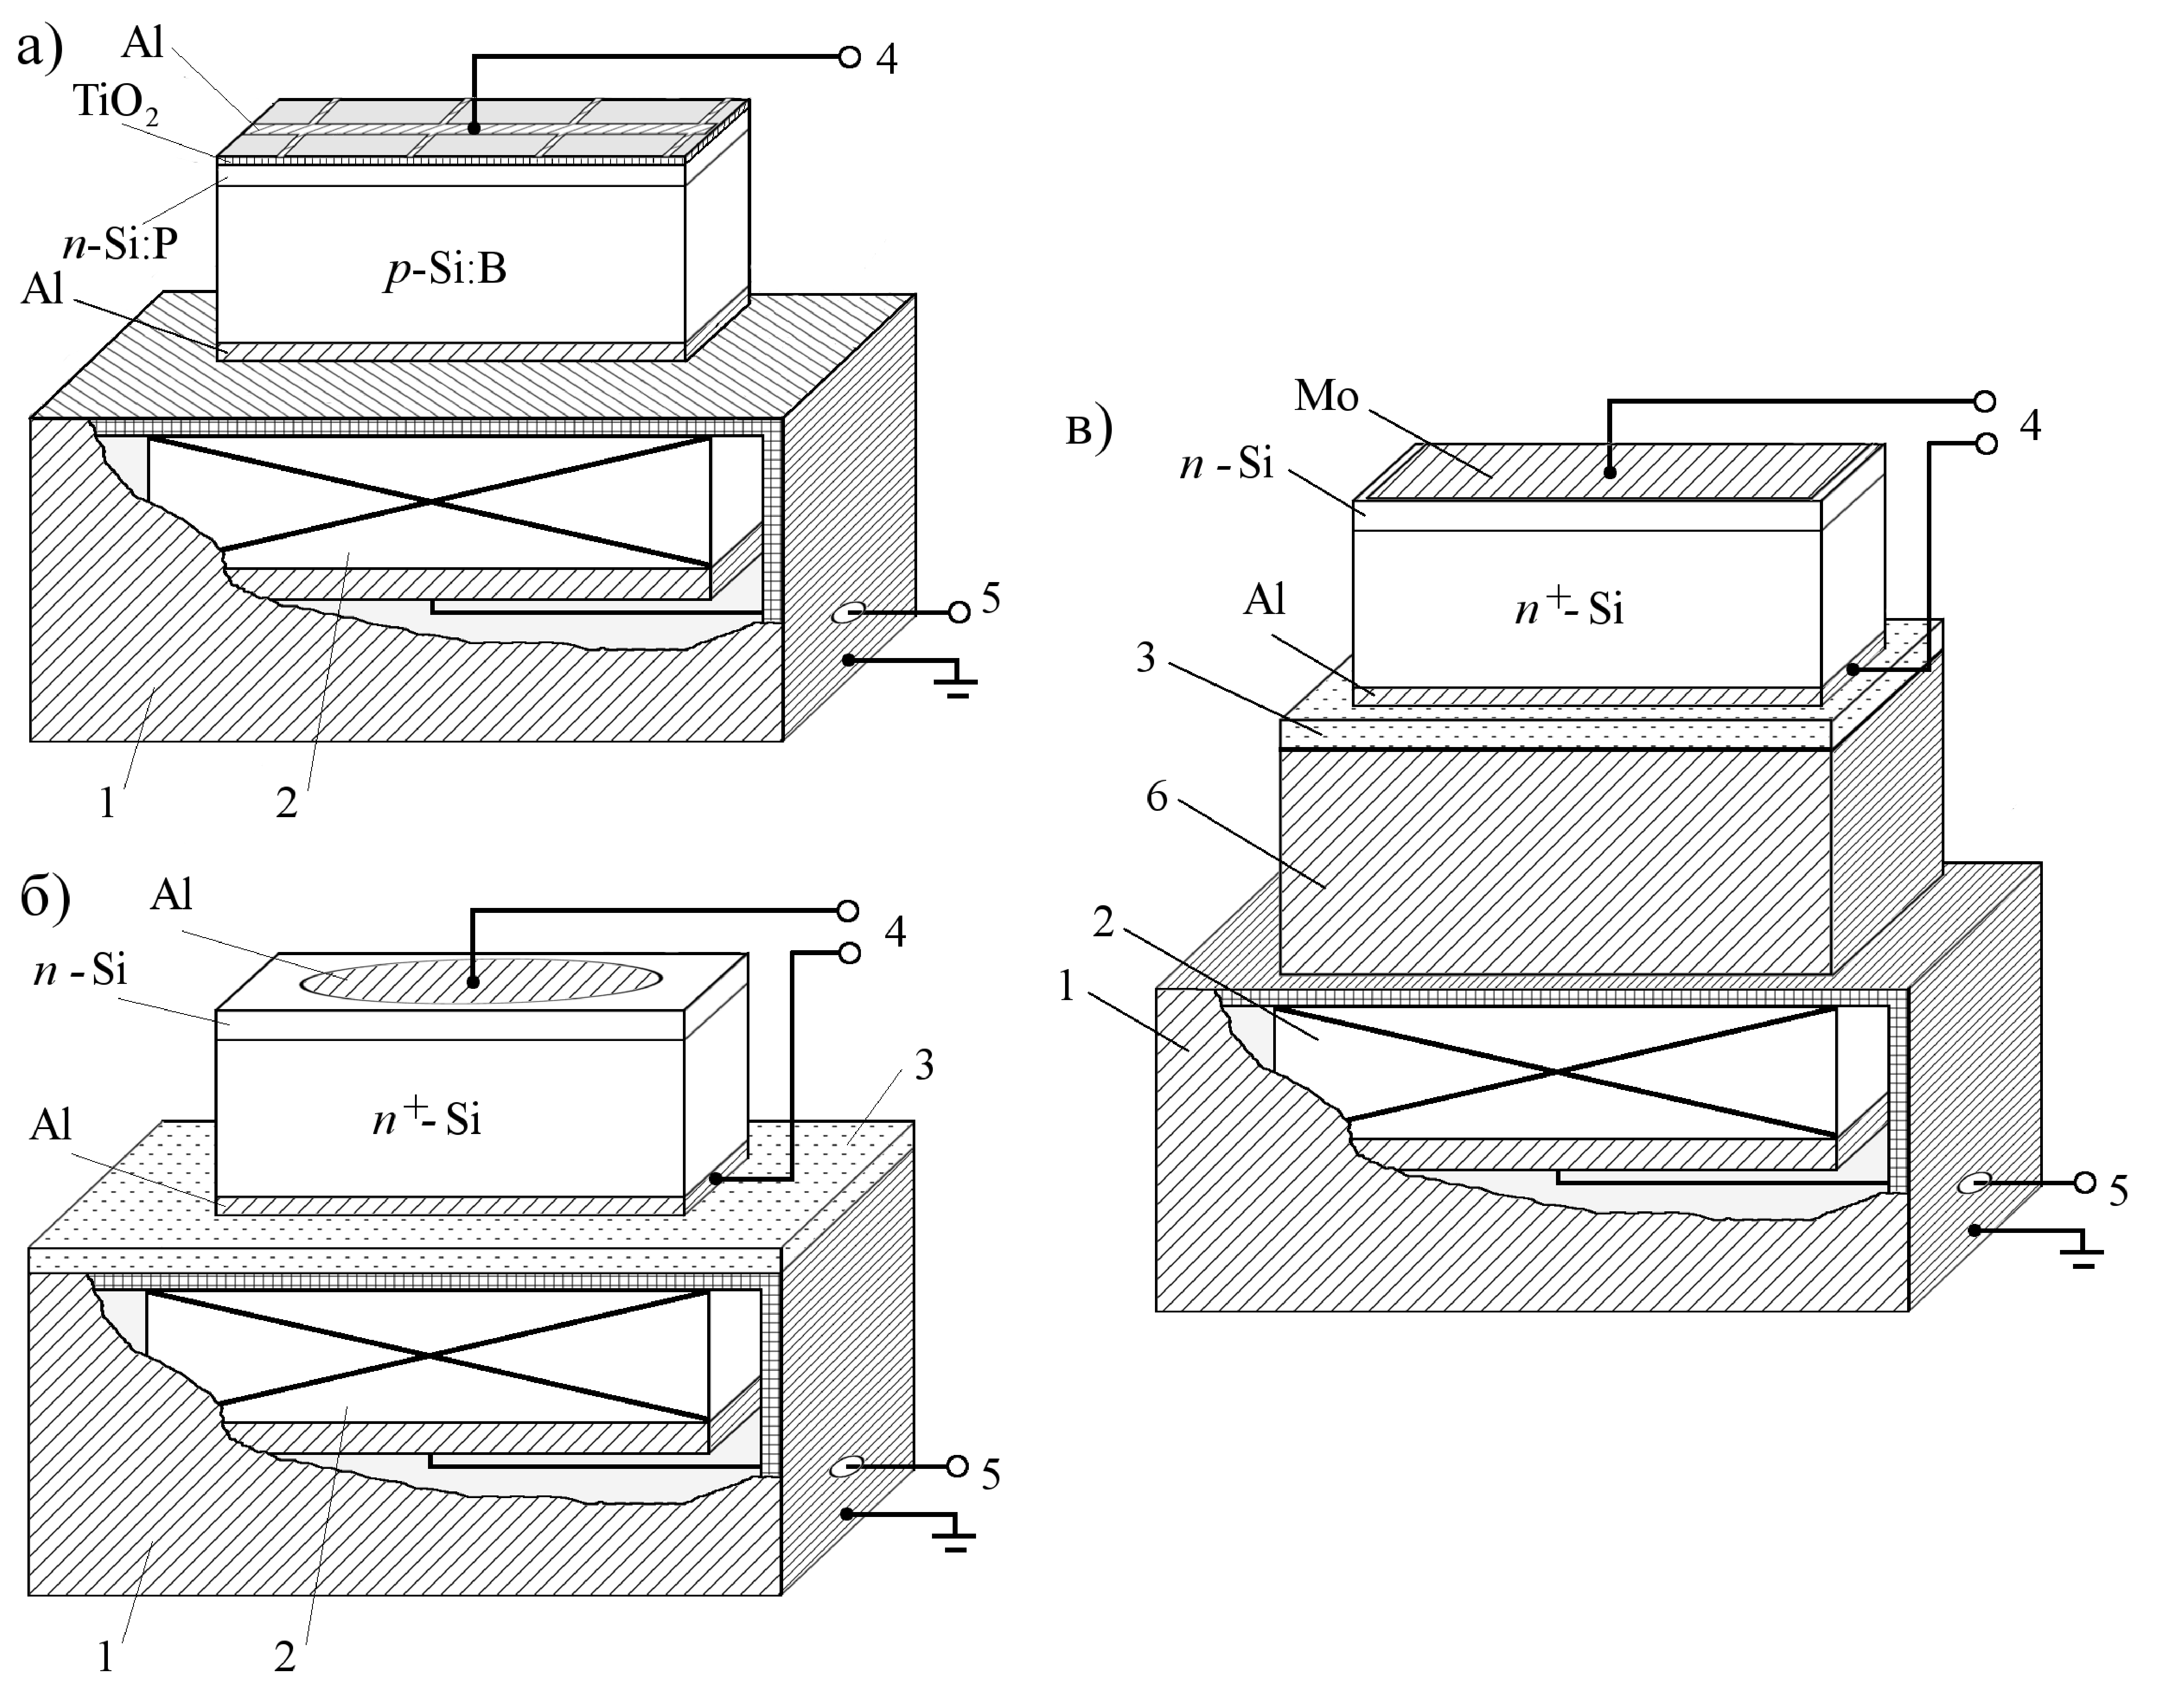
\includegraphics[width=1.0\textwidth]{USL}%
\caption{\label{figUSL}
Використані схеми УЗН.
1 --  екран (алюмінієва фольга, товщина 0,012 мм);
2 --- п'єзоелектричний перетворювач (LiNbO$_3$);
3 --- діелектричний прошарок (слюда, товщина 0,03 мм);
4 --- контакти для вимірювання ВАХ;
5 --- контакти для збудження УЗ;
6 --- буфер (циліндр Al з високим ступенем паралельності граней, довжина 2~см)
}
\end{figure}

Структури, в яких проводилися дослідження ефектів УЗН, містили енергетичний бар'єр, пов'язаний з наявністю контакту МН або p--n переходу і розміщений поблизу однієї з поверхонь зразка.
Введення УЗ відбувалось з боку грані, протилежної до місця розташування бар'єру.
Тобто, напрям поширення АХ перпендикулярний площині бар'єру і співпадає з напрямом струму, який виникає під час прикладення до структури електричної напруги (або при освітленні, якщо об'єктом дослідження є сонячний елемент).
При цьому, при використанні повздовжніх хвиль вимушені зміщення атомів відбуваються у тому самому напрямі, тоді як для поперечних хвиль коливання частинок спрямовані перпендикулярно до електричного струму у площині бар'єру.


Для створення акустичного контакту при різних УЗН використовувалися вакуумне масло, клей БФ6, піцеїн.
Зауважимо, що у випадку низькотемпературного (при $T<230$~К) УЗН процес збудження АХ був утруднений через те, що
рідкі акустичні склейки на кшталт вакуумного масла кристалізувалися і переставали виконувати свою функцію.
В той же час, контакт створений при кімнатній температурі за допомогою жорсткої склейки (піцеїн або БФ6),
руйнувався при охолодженні внаслідок різниці коефіцієнтів теплового розширення.
В роботі проведення низькотемпературних УЗН при використанні повздовжніх хвиль здійснювалось за допомогою свіжого (до 5~год після нанесення) контакту з клею БФ6, який ще не висох.
Наявність акустичного контакту контролювалася за виглядом залежності повного опору перетворювача від частоти (АЧХ, амплітудно--частотної характеристики).
Зокрема, при використанні схеми, зображеної на Рис.~\ref{figUSL},в, за наявності акустичного контакту на АЧХ з'являвся ряд максимумів, пов'язаних з відбиванням хвиль від граней буфера.


Раніше показано \cite{Ostapenko1995,YOlikhTPL2011,Ostrovskii2001}, що характерний час зміни властивостей кремнієвих структур під дією УЗ не перевищує $2\cdot10^3$~c.
Для того, щоб дочекатися закінчення всіх перехідних АІ процесів, використовувалася наступна експериментально процедура.
УЗН починалась при кімнатній температурі.
Після цього зразки перебували не менше 60~хв за умов поширення в них пружних коливань і лише після цього, не припиняючи дії УЗ, починалось вимірювання електрофізичних параметрів та/або процеси нагріву або охолодження.

Відомо, що під час навантаження п'єзоперетворювач нагрівається.
Температура кремнієвих структур контролювалася диференційною термопарою мідь--константан.
В роботі проводилось порівняння значень параметрів, отриманих за однакових температур в умовах УЗН зразків та без нього.
Це дозволяло виокремити АІ зміни характеристик напівпровідникових структур, від змін, пов'язаних з їх розігрівом під час УЗН.
Для оцінки величини впливу УЗ на певний параметр $P$ (яким могла бути напруга холостого ходу, фактор неідеальності, величина зворотного струму тощо),
використовувалися його абсолютні
 \begin{equation}
 \label{eqAbsDelta}
\Delta P=P_{in}-P_\mathtt{US}
 \end{equation}
чи відносні зміни
 \begin{equation}
 \label{eqEpsDelta}
\varepsilon_P=\frac{P_{in}-P_\mathtt{US}}{P_{in}},
 \end{equation}
де нижні індекси <<$\mathtt{US}$>> та <<$in$>> вказують на те, що відповідне значення параметра було отримане при однаковій температурі за умов УЗН та без нього, відповідно.

Таким чином, основними параметрами УЗН є $f_\mathtt{US}$, тип збуджених хвиль, $W_\mathtt{US}$ та температура зразка під час поширення АХ.
Параметри УЗН, які використовувалася в тих чи інших дослідах, зазначено на початку відповідного розділу.

При УЗО процеси впливу АХ та вимірювання параметрів були розділені в часу і тому нагальної необхідності екранування п'єзоелектричних полів не було.
Як наслідок, експериментальна схема простіша, п'єзоперетворювач безпосередньо акустично контактував з досліджуваною структурою.


\section{Оцінка параметрів акустичного впливу\label{subLowT}}
Для оцінки інтенсивності АХ введеної, наприклад, у кремнієву структуру використовувалася формула плоского п’єзоперетворювача \cite{WusBook}:
 \begin{equation}
 \label{eqWus}
 W_\mathtt{US}=4K_\mathtt{LNO}^2C_\mathtt{LNO}f_r\frac{\rho_\mathtt{LNO}\,\upsilon_\mathtt{LNO}}{\rho_\mathtt{Si}\,\upsilon_\mathtt{Si}}\frac{V_\mathtt{RF}^2}{A_\mathtt{LNO}M_0},
 \end{equation}
де
$K_\mathtt{LNO}$ --- коефіцієнт електромеханічного зв'язку,
$C_\mathtt{LNO}$ та $A_\mathtt{LNO}$ --- статична ємність закріпленого перетворювача та його площа, відповідно;
для використаних в роботі перетворювачів ємність складала $(1\div3)\cdot10^{-10}$~Ф залежно від площі та товщини;
$f_r$ --- резонансна частота;
$\rho_\mathtt{LNO}$ та $\rho_\mathtt{Si}$ --- густина LiNbO$_3$ та кремнію, відповідно;
$\upsilon_\mathtt{LNO}$ та $\upsilon_\mathtt{Si}$ --- швидкості поширення звуку в ніобаті літію та Si, відповідно;
$V_\mathtt{RF}$ --- амплітуда високочастотної напруги, прикладеної до перетворювача,
а коефіцієнт $M_0$ розраховується за допомогою співвідношення
 \begin{equation}
 \label{eqM0}
 M_0=\frac{\left[\cos\left(\pi\frac{f_\mathtt{US}}{f_r}\right)\right]^2+\left[\frac{\rho_\mathtt{LNO}\,\upsilon_\mathtt{LNO}}{\rho_\mathtt{Si}\,\upsilon_\mathtt{Si}}\sin\left(\pi\frac{f_\mathtt{US}}{f_r}\right)\right]^2}
 {\left[\sin\left(\frac{\pi}{2}\frac{f_\mathtt{US}}{f_r}\right)\right]^4}.
 \end{equation}
При цьому при поширенні АХ має місце відносна деформація
 \begin{equation}
 \label{eqDefUS}
 \xi_{\mathtt{US}}=\sqrt{\frac{2W_\mathtt{US}}{\rho_\mathtt{Si}\,\upsilon_\mathtt{Si}^3}},
 \end{equation}
а амплітуда зміщень атомів
 \begin{equation}
 \label{eqAmpUS}
 u_{\mathtt{US}}=\sqrt{\frac{W_\mathtt{US}}{2\,\pi^2\,f_\mathtt{US}^2\,\rho_\mathtt{Si}\,\upsilon_\mathtt{Si}}}.
 \end{equation}

Значення резонансної частоти перетворювачів визначалось за допомогою приладу для дослідження АЧХ Х1--38.
Параметри, які використовувалися при розрахунках, наведено в Таблиці~\ref{tabLNO}.


\begin{table}
\caption{\label{tabLNO}Деякі параметри ніобату літію та кремнію при кімнатній температурі \cite{WusBook,ShackBook}.
}
%\begin{tabular}{|l|l|c|}
%\begin{tabularx}{\textwidth}{|>{\raggedright\arraybackslash}X|>{\centering\arraybackslash}X|>{\centering\arraybackslash}X|}
\begin{tabularx}{\textwidth}{|l|>{\centering\arraybackslash}X|>{\centering\arraybackslash}X|}
\hline
$K_\mathtt{LNO}^2$&зріз $(Y\!+\!36^\circ)$&0,24\\
\cline{2-3}
&зріз &0,46\\
\hline
$\upsilon_\mathtt{LNO}$,&повздовжні хвилі&7340\\
\cline{2-3}
м/с&поперечні хвилі&4560\\
\hline
$\upsilon_\mathtt{Si}$,&повздовжні хвилі&8430\\
\cline{2-3}
м/с&поперечні хвилі&5840\\
\hline
\multicolumn{2}{|l|}{$\rho_\mathtt{LNO}$, кг/м$^3$}&4700\\
\hline
\multicolumn{2}{|l|}{$\rho_\mathtt{Si}$, кг/м$^3$}&2328\\
\hline
%\end{tabular}
\end{tabularx}
\end{table}

Під час проведенні УЗН за схемами, наведеними на Рис.~\ref{figUSL},а  та Рис.~\ref{figUSL},б дослідження проводились у достатньо вузькому температурному діапазоні $290\div340$~К.
При цьому вважалось, що параметри п'зоелектричного перетворювача змінюються мало, сталість величини $V_\mathtt{RF}$ забезпечує незмінність $W_\mathtt{US}$  для всього діапазону температур, і для оцінки параметрів ультразвукового навантаження використовувалися формули
(\labelcref{eqAmpUS,eqWus,eqM0,eqDefUS}).
Вплив металевого екрануючого шару та діелектричного слюдяного прошарку на інтенсивність звуку, введеного в зразок, вважався знехтувано малим, так як їх товщина значно менша ніж половина довжини АХ.
В той же час, подібні спрощення не є виправданими у випадку, коли коли використовується схема УЗН, показана на Рис.~\ref{figUSL},в і вимірювання проводяться в широкому температурному діапазоні.
%Більш детально процедура оцінки $W_\mathtt{US}$ в цьому випадку описана в наступному розділі \ref{subLowT}.




\chapter{Динамічні акусто--індуковані ефекти в радіаційно опромінених та неопромінених кремнієвих структурах з p--n переходом\label{Ch_SSC}}


\section{Особливості використання активного ультразвуку}
Значна частина представлених у дисертаційній роботі результатів (розділи~\ref{Ch_SSC}, \ref{Ch_GammaSD}, \ref{Ch_USL_T_SD} та \ref{Ch_UST_MW}) пов'язана з дослідженням ефектів, які відбуваються в напівпровідникових структурах внаслідок
поширення в них акустичних хвиль (АХ) мегагерцевого діапазону.
У зв'язку з тим, що використання ультразвуку (УЗ), на жаль, ще не є стандартним способом впливу на напівпровідникові кристали,
у цьому параграфі представлено узагальнена  інформація щодо відповідних експериментальних методик.

Зокрема, представлені описи процедур ультразвукової обробки (УЗО) та ультразвукового навантаження (УЗН).
Відмінності у використанні цих термінів пов'язані з оборотністю АІ процесів.
Так, в першому випадку (УЗО), внаслідок поширення пружних хвиль відбуваються незворотні (залишкові) зміни властивостей напівпровідникових структур.
Тоді як в другому випадку (УЗН), ефекти є оборотніми (динамічними), зміни електрофізичних параметрів спостерігаються лише за умов поширення АХ;
після припинення дії УЗ параметри поступово повертаються до своїх вихідних (до початку УЗН) значень.

Для збудження УЗ у досліджуваних структурах використовувалися п'єзоелектричні перетворювачі,
виготовлені з пластин ніобату літію (LiNbO$_3$) з металізацією обох граней шляхом вакуумного напилення алюмінію.
Для збудження повздовжніх та поперечних акустичних хвиль використовувалися пластини зі зрізами $(Y\!+\!36^\circ)$ та $(Y\!+\!163^\circ)$, відповідно.

З літератури \cite{Ostapenko1995,Davletova2008,Davletova2009,Pashaev2014r} відомо, що АХ з частотою, що знаходиться в діапазоні $1\div30$~МГц, здатні впливати на стан дефектів у кремнії.
Саме такий частотний діапазон був використаний у дослідженнях, результати яких представлені далі.
В експериментах проводилось збудження УЗ з частотою $f_\mathtt{US}$, яка знаходилась поблизу першої або третьої гармоніки товщинного резонансу пластинки.
Значення резонансної частоти перетворювачів визначалось за допомогою приладу для дослідження АЧХ Х1--38.
Безпосереднє значення $f_\mathtt{US}$, при якому введення пружних коливань у зразок відбувається найбільш ефективно, визначалось стандартним методом за максимальною амплітудою коливань краплі води (або вакуумного масла), розміщеної на поверхні перетворювача, при прикладанні до його граней змінної напруги.

Попередні дослідження різних авторів \cite{Davletova2008,Davletova2009,Pashaev2014r,Vlasov2009r} показали, що використання УЗ
з інтенсивністю, як правило, $W_\mathtt{US}\geq3$~Вт/см$^2$ спричинює необоротні (залишкові) зміни властивостей кремнієвих структур.
Ці процеси можуть бути пов'язані з відпалом радіаційних дефектів, формуванням нових дефектів або переміщенням вже існуючих, на відстані, що значно перевищують міжатомну відстань.
Так як метою частини роботи (розділи~\ref{Ch_SSC}, \ref{Ch_GammaSD} та \ref{Ch_USL_T_SD}) було дослідження саме оборотних АІ ефектів,
то переважна більшість УЗН проводилась при $W_\mathtt{US} \leq 1$~Вт/см$^2$.
Детальніше процедура оцінки $W_\mathtt{US}$ та інших параметрів УЗ впливу наведена у параграфах \ref{SC:USL} та \ref{SSDB:USL}.

Для того, щоб під час УЗН позбавитися впливу п'єзоелектричного поля, яке супроводжує механічні коливання пластини LiNbO$_3$,  як на параметри напівпровідникових структур, так і на процес вимірювання електрофізичних параметрів,
перетворювач екранувався.
Як наслідок, можна стверджувати, що виявлені під час УЗН ефекти визначаються лише знакозмінною деформацією.
Для створення акустичного контакту при різних УЗН використовувалися вакуумне масло, клей БФ6, піцеїн.
Детальні схеми акустичного навантаження зразків наведено у кожному розділі.


Структури, в яких проводилися дослідження ефектів УЗН, містили енергетичний бар'єр, пов'язаний з наявністю контакту МН або $p-n$ переходу, розміщений поблизу однієї з поверхонь зразка.
Введення УЗ відбувалось з боку грані, протилежної до місця розташування бар'єру.
Тобто, напрям поширення АХ перпендикулярний площині бар'єру і збігається з напрямом струму, який виникає під час прикладення до структури електричної напруги (або при освітленні, якщо об'єктом дослідження є сонячний елемент).
При цьому, при використанні повздовжніх хвиль вимушені зміщення атомів відбуваються у тому самому напрямі, тоді як для поперечних хвиль коливання частинок спрямовані перпендикулярно до електричного струму у площині бар'єру.

Раніше показано \cite{Ostapenko1995,YOlikhTPL2011,Ostrovskii2001}, що характерний час зміни властивостей кремнієвих структур під дією УЗ не перевищує $2\cdot10^3$~c.
Для того, щоб дочекатися закінчення всіх перехідних АІ процесів, використовувалася наступна експериментально процедура.
УЗН починалося при кімнатній температурі.
Після цього зразки перебували не менше 60~хв за умов поширення в них пружних коливань і лише після цього, не припиняючи дії УЗ, починалися вимірювання електрофізичних параметрів та/або процеси нагріву або охолодження.

Відомо, що під час навантаження п'єзоелектричний перетворювач нагрівається.
Температура структур, які досліджувалися, контролювалася диференційною термопарою мідь--константан.
В роботі проводилось порівняння значень параметрів, отриманих за однакових температур в умовах УЗН зразків та без нього.
Це дозволяло виокремити АІ зміни характеристик напівпровідникових структур, від змін, пов'язаних з їх розігрівом під час УЗН.
Для оцінки величини впливу УЗ на певний параметр $P$ (яким могла бути напруга холостого ходу, фактор неідеальності, величина зворотного струму тощо),
використовувалися його абсолютні
 \begin{equation}
 \label{eqAbsDelta}
\Delta P=P_{in}-P_\mathtt{US}
 \end{equation}
чи відносні зміни
 \begin{equation}
 \label{eqEpsDelta}
\varepsilon_P=\frac{P_{in}-P_\mathtt{US}}{P_{in}},
 \end{equation}
де нижні індекси <<$\mathtt{US}$>> та <<$in$>> вказують на те, що відповідне значення параметра було отримане при однаковій температурі за умов УЗН та без нього, відповідно.

При УЗО процеси впливу АХ та вимірювання параметрів були розділені в часу і тому нагальної необхідності екранування п'єзоелектричних полів не було.
Як наслідок, експериментальна схема простіша, п'єзоперетворювач безпосередньо акустично контактував з досліджуваною структурою.




\section{Структура кремнієвих сонячних елементів та режими їх радіаційного опромінення\label{SSC}}
Сонячні елементи, які досліджувалися в роботі, були створені на основі пластин кремнію діаметром близько 100~мм.
Пластини  товщиною 300~мкм з орієнтацією (111) були вирізані зі злитків, вирощених за методом Чохральського.
Легування здійснювалось шляхом додавання у розплав атомів бору (кремній марки КДБ10).
У дослідженому температурному діапазоні концентрація основних носіїв заряду складала величину $p_p=1,4\cdot10^{15}$~см$^{-3}$.
% та $p_p=4.5\cdot10^{15}$~см$^{-3}$).

Для створення $n^+$ емітера проводилась імплантація іонів фосфору, після закінчення якої було проведено активізуючий відпал.
Як наслідок, був створений шар з електронною провідністю товщиною близько  0,5~мкм з концентрацією вільних носіїв заряду $10^{19}$~см$^{-3}$.

Поверхня пластини була пасивована шляхом нанесення плівки Al$_2$O$_3$.
Крім того, на фронтальну поверхню був нанесений антивідбиваючий шар діоксиду титану (TiO$_2$) з використанням методу APCVD (atmospheric pressure chemical  vapour  deposition).
З використанням методу трафаретного друку (screen printing) було створено омічні алюмінієві електроди (суцільний на задній поверхні та металева сітка на передній).
Нарешті, був проведений швидкий відпал отриманих структур при температурі $800^\circ$C тривалістю декілька хвилин.
Структура досліджених кремнієвих сонячних елементів (КСЕ) зображена на Рис.~\ref{figSSC},а.
Зауважимо, що цей рисунок наведено без збереження масштабних співвідношень між окремими частинами.

Для досліджень використовувалися зразки площею $1,5\div2,1$~cm$^{2}$, вирізані з різних (переважно центральних) областей пластини.
Принагідно зауважимо, що, як показують дані робіт \cite{Breitenstein2013,SC:Area}, для КСЕ з площею, яка
перевищує 100~мм$^2$, ні густина струму, ні питомий опір не залежать від розміру структури,
тобто для зразків із такою площею крайовими ефектами можна знехтувати.
Для позначення зразків надалі використовується запис на кшталт SSC$x$, де $x$ --- номер зразка.
Місце розташування зразків на вихідній пластині показано на Рис.~\ref{figSSC},б.

\begin{figure}
\center
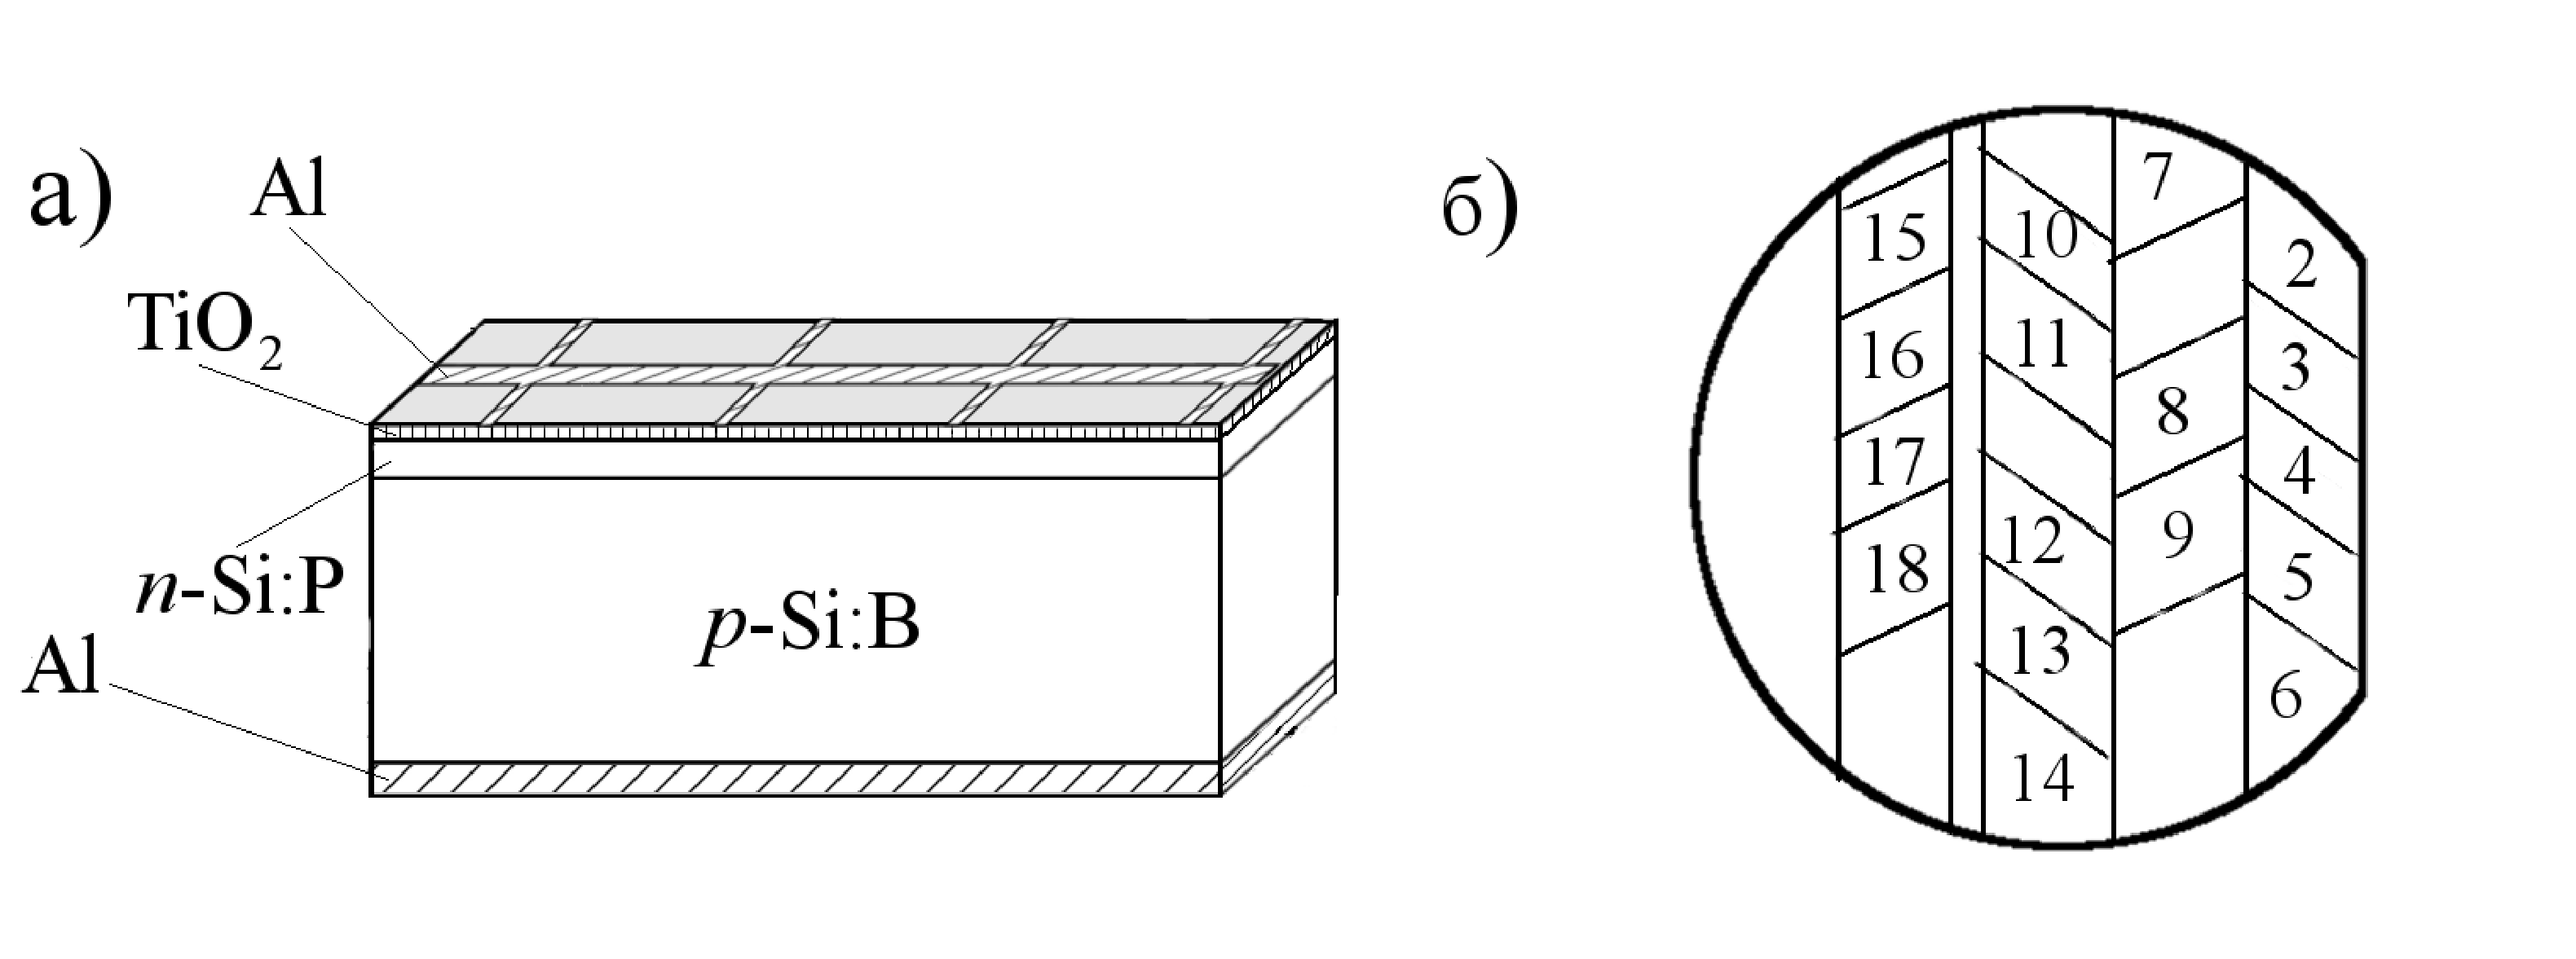
\includegraphics[width=1.0\textwidth]{SSC}%
\caption{\label{figSSC}
Структура кремнієвих сонячних елементів (а) та місце розташування зразків (б).
}
\end{figure}


\begin{table}[b]
\caption{\label{tabSSCSample}Параметри опромінених кремнієвих сонячних елементів.
}
\begin{tabular}{|c|c|c|c|c|c|}
%\begin{tabularx}{\textwidth}{|>{\centering\arraybackslash}X|
%                             >{\centering\arraybackslash}X|
%                            >{\centering\arraybackslash}X|
%                            >{\centering\arraybackslash}X|
%                            >{\centering\arraybackslash}X|
%                            >{\centering\arraybackslash}X|
%                            }
\hline
\multirow{2}{*}{Зразок} &Тип&$D$,&$\Psi$, &NIEL,& $D_d$,  \\
&опромінення& рад& см$^{-2}$&MеВ$\cdot$см$^2$/г& MеВ/г \\
\hline
nSC4&нейтрони&4,5$\cdot$10$^3$&4$\cdot$10$^{11}$&2,04$\cdot$10$^{-3}$&8,2$\cdot$10$^{8}$\\ \hline
g6SC8&$\gamma$--$^{60}$Co&1$\cdot$10$^6$&1,6$\cdot$10$^{15}$&$(1,07\div1,31)\cdot10^{-7}$&$(1,7\div2,1)\cdot 10^{8}$\\
\cline{1-4}
\cline{6-6}
g7SC12&$\gamma$--$^{60}$Co&1$\cdot$10$^7$&1,6$\cdot$10$^{16}$&\cite{NIEL:Akkerman,NIEL:Messenger,NIEL:Allam}&$(1,7\div2,1)\cdot 10^9$\\ \hline
\end{tabular}
%\end{tabularx}
\end{table}

Частина зразків, використаних для досліджень, була опромінена або реакторними нейтронами, або гамма--квантами $^{60}$Co.
Флюєнс $\Psi$ нейтронного опромінення складав $4\cdot10^{11}$~см$^{-2}$,
для позначення нейтронно опромінених зразків використовується префікс <<n>> (наприклад <<nSC4>>).
Доза $D$ опромінення гамма-квантами дорівнювала $10^6$ або $10^7$~рад, для позначення відповідних зразків використовуються префікси <<g6>> та <<g7>>, відповідно.

Значення доз та флюєнсів наведено в Таблиці~\ref{tabSSCSample}.
Для визначення кореляцій між $D$ та $\Psi$ для нейтронного та $\gamma-^{60}$Co опромінення використовувалися дані робіт \cite{NIEL:Akkerman,Brauning}.
У цій таблиці також наведено дані щодо величини NIEL (non--ionizing energy losses, енергетичні втрати, не пов'язані з іонізацією) при поширенні нейтронів та гамма--квантів $^{60}$Co в кристалах кремнію.
NIEL характеризує втрати енергії налітаючої частинки на одиницю довжини шляху, пов'язані зі зміщенням атомів ґратки \cite{NIEL:Huhtinen,NIEL:Messenger}, тобто, фактично, процеси радіаційного дефектоутворення.
Зокрема, вважається що радіаційне ушкодження кристалів характеризується такою величиною, як $D_d=\Psi\cdot \mbox{NIEL}$ (displacement damage dose) \cite{NIEL:Messenger}.
Величини $D_d$ для досліджених структур також розміщені у Таблиці~\ref{tabSSCSample}.
З наведених даних видно, що як при використанні нейтронів, так і $\gamma$--квантів очікуване пошкодження кристалічної структури є близьким.
Проте, як відомо,  опромінення різного типу викликає появу різних за структурою дефектів.
Зокрема, $\gamma$--промені викликають появу, переважно, А--центрів \cite{NIEL:Jafari,Gamma:Prabhakara,NIEL:Moll}, тоді як нейтрони призводять до появи вакансійних кластерів\cite{Rew:Srour,Junkes}, областей розупорядкування  \cite{Neutron:Arutyunov} та комплексів C$_i$O$_i$ \cite{NIEL:Moll,neutron:Londos}.
Більш детально це питання розглянуте у розділі~\ref{Rad_SSC}.

Відомо \cite{RadBook}, що після радіаційного опромінення, особливо нейтронного, \cite{NIEL:Moll,Rew:Srour} у кристалах кремнію відбуваються довготривалі перехідні процеси, пов'язані з утворенням вторинних радіаційних дефектів (РД).
Для того, щоб уникнути впливу подібних процесів зразки після опромінення перед початком досліджень, результати який наведено далі, зберігались протягом п'яти років при кімнатній температурі.




\section{Режими ультразвукового навантаження кристалічних кремнієвих сонячних елементів\label{SC:USL}}
Схема акустичного навантаження зразків наведено на Рис.~\ref{figUSL:SC}.
Акустичний контакт створювався за допомогою вакуумного масла при використанні повздовжніх хвиль та клею БФ6 --- для поперечних.

\begin{figure}
\center
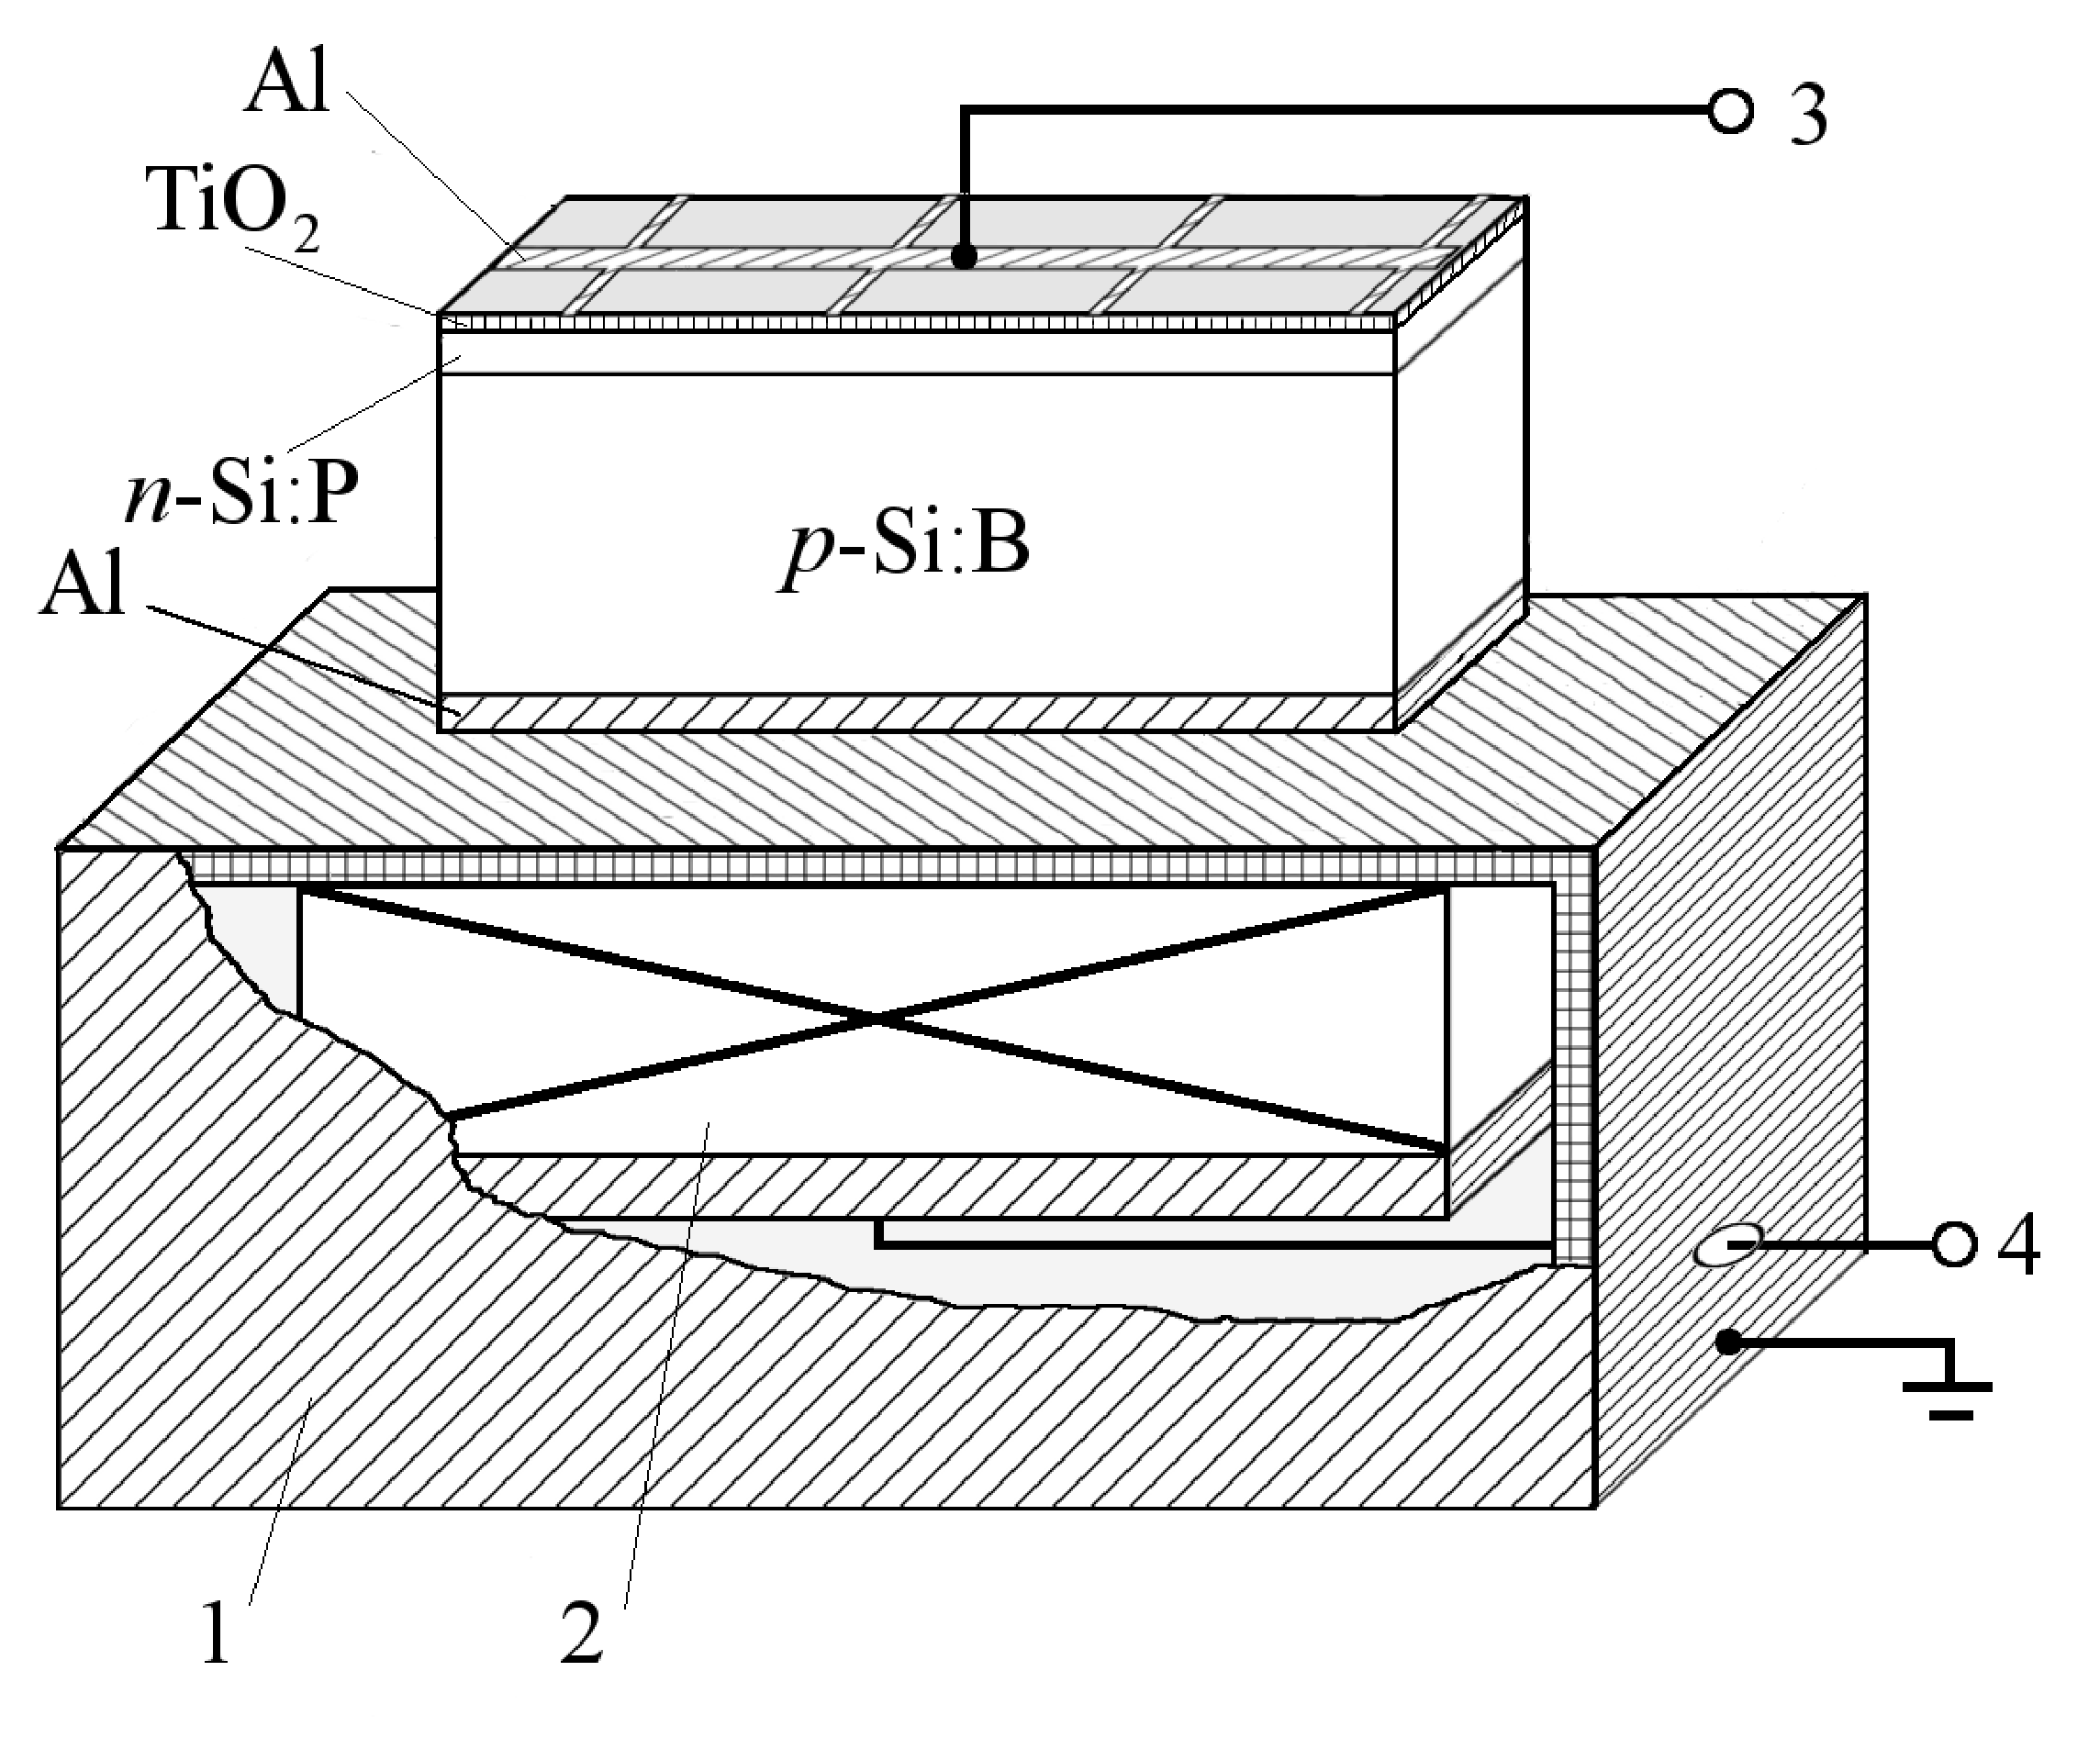
\includegraphics[width=0.6\textwidth]{USL_SC}%
\caption{\label{figUSL:SC}
Cхема УЗН кремнієвих сонячних елементів.
1 --  екран (алюмінієва фольга, товщина 0,012 мм);
2 --- п'єзоелектричний перетворювач (LiNbO$_3$);
3 --- контакти для вимірювання ВАХ;
4 --- контакти для збудження УЗ.
}
\end{figure}


Для оцінки інтенсивності АХ введеної у кремнієву структуру використовувалася формула плоского п’єзоперетворювача \cite{WusBook}:
 \begin{equation}
 \label{eqWus}
 W_\mathtt{US}=4K_\mathtt{LNO}^2C_\mathtt{LNO}f_r\frac{\rho_\mathtt{LNO}\,\upsilon_\mathtt{LNO}}{\rho_\mathtt{Si}\,\upsilon_\mathtt{Si}}\frac{V_\mathtt{RF}^2}{A_\mathtt{LNO}M_0},
 \end{equation}
де
$K_\mathtt{LNO}$ --- коефіцієнт електромеханічного зв'язку,
$C_\mathtt{LNO}$ та $A_\mathtt{LNO}$ --- статична ємність закріпленого перетворювача та його площа, відповідно;
для використаних в роботі перетворювачів ємність складала $(1\div3)\cdot10^{-10}$~Ф залежно від площі та товщини;
$f_r$ --- резонансна частота;
$\rho_\mathtt{LNO}$ та $\rho_\mathtt{Si}$ --- густина LiNbO$_3$ та кремнію, відповідно;
$\upsilon_\mathtt{LNO}$ та $\upsilon_\mathtt{Si}$ --- швидкості поширення звуку в ніобаті літію та Si, відповідно;
$V_\mathtt{RF}$ --- амплітуда високочастотної напруги, прикладеної до перетворювача,
а коефіцієнт $M_0$ розраховується за допомогою співвідношення
 \begin{equation}
 \label{eqM0}
 M_0=\frac{\left[\cos\left(\pi\frac{f_\mathtt{US}}{f_r}\right)\right]^2+\left[\frac{\rho_\mathtt{LNO}\,\upsilon_\mathtt{LNO}}{\rho_\mathtt{Si}\,\upsilon_\mathtt{Si}}\sin\left(\pi\frac{f_\mathtt{US}}{f_r}\right)\right]^2}
 {\left[\sin\left(\frac{\pi}{2}\frac{f_\mathtt{US}}{f_r}\right)\right]^4}.
 \end{equation}
При цьому при поширенні АХ має місце відносна деформація
 \begin{equation}
 \label{eqDefUS}
 \xi_{\mathtt{US}}=\sqrt{\frac{2W_\mathtt{US}}{\rho_\mathtt{Si}\,\upsilon_\mathtt{Si}^3}},
 \end{equation}
а амплітуда зміщень атомів
 \begin{equation}
 \label{eqAmpUS}
 u_{\mathtt{US}}=\sqrt{\frac{W_\mathtt{US}}{2\,\pi^2\,f_\mathtt{US}^2\,\rho_\mathtt{Si}\,\upsilon_\mathtt{Si}}}.
 \end{equation}

Параметри, які використовувалися при розрахунках, наведено в Таблиці~\ref{tabLNO}.


\begin{table}
\caption{\label{tabLNO}Деякі параметри ніобату літію та кремнію при кімнатній температурі \cite{WusBook,ShackBook}.
}
%\begin{tabular}{|l|l|c|}
%\begin{tabularx}{\textwidth}{|>{\raggedright\arraybackslash}X|>{\centering\arraybackslash}X|>{\centering\arraybackslash}X|}
\begin{tabularx}{\textwidth}{|l|>{\centering\arraybackslash}X|>{\centering\arraybackslash}X|}
\hline
$K_\mathtt{LNO}^2$&зріз $(Y\!+\!36^\circ)$&0,24\\
\cline{2-3}
&зріз $(Y\!+\!163^\circ)$&0,46\\
\hline
$\upsilon_\mathtt{LNO}$,&повздовжні хвилі&7340\\
\cline{2-3}
м/с&поперечні хвилі&4560\\
\hline
&повздовжні хвилі, $[100]$&8430\\
\cline{2-3}
&повздовжні хвилі, $[111]$&9850\\
\cline{2-3}
$\upsilon_\mathtt{Si}$,&повздовжні хвилі, $[110]$&9130\\
\cline{2-3}
м/с&поперечні хвилі, $[110]\,/\,[1\bar{1}0]$&4670\\
\cline{2-3}
&поперечні хвилі, $[110]\,/\,[001]$&5840\\
\cline{2-3}
&поперечні хвилі, $[111]\,/\,$довіл.&5090\\
\hline
\multicolumn{2}{|l|}{$\rho_\mathtt{LNO}$, кг/м$^3$}&4700\\
\hline
\multicolumn{2}{|l|}{$\rho_\mathtt{Si}$, кг/м$^3$}&2328\\
\hline
%\end{tabular}
\end{tabularx}
\end{table}

Дослідження проводились у достатньо вузькому температурному діапазоні $290\div340$~К.
При цьому вважалось, що параметри п'зоелектричного перетворювача змінюються мало, сталість величини $V_\mathtt{RF}$ забезпечує незмінність $W_\mathtt{US}$  для всього діапазону температур.
Вплив металевого екрануючого прошарку на інтенсивність звуку, введеного в зразок, вважався знехтувано малим, так як їх товщина значно менша ніж половина довжини АХ.



Параметри УЗ навантажень КСЕ, їх позначення та зразки, до яких вони застосовувалися, наведено в Таблиці~\ref{tabUSL}.

\begin{table}
\caption{\label{tabUSL}Параметри ультразвукових навантажень КСЕ.
}
%\center
\begin{tabular}{|c|c|c|c|c|c|c|c|}
\hline
$f_\mathtt{US}$,&Тип&$W_{\mathtt{US}}$,&$\xi_{\mathtt{US}}$,&$u_{\mathtt{US}}$,&$T$,&УЗН&Зразок\\
МГц&хвиль&Вт/см$^2$&$10^{-6}$&нм&K&&\\
\hline
8,0&повздовжні&0,18&1,3&0,30&302$\div$333&U--L&SC11, SC17\\ \hline
4,2&поперечні&0,19&2,9&0,63&300$\div$340&U--Ts1&SC17, g7SC12\\ \hline
4,2&поперечні&0,22&3,1&0,67&295$\div$335&U--Ts2&SC11\\ \hline
4,2&поперечні&0,24&3,2&0,70&300$\div$340&U--Ts3&nSC4\\ \hline
4,2&поперечні&0,37&4,0&0,87&308$\div$340&U--Tb1&g7SC12\\ \hline
4,2&поперечні&0,38&4,1&0,89&308$\div$340&U--Tb2&g6SC8\\ \hline
4,2&поперечні&0,40&4,2&0,91&310$\div$340&U--Tb3&SC11, SC17\\
&&&&&&&nSC4\\ \hline
8,0&повздовжні&до 1,5&до 5,1&до 0,86&290$\div$330&U--L8&SC13, nSC7\\ \hline
26,1&повздовжні&до 0,26&до 1,9&до 0,1&290$\div$333&U--L26&SC13, nSC7\\ \hline
%4,1&повздовжні&0,02& 0,7& 0,19&$\sim$300&U--L4t&SC3\\ \hline
%4,1&повздовжні&0,18& 1,6& 0,52&$\sim$300&U--L4t&SC3\\ \hline
%4,1&повздовжні&0,30& 2,1& 0,68&$\sim$300&U--L4t&SC3\\ \hline
%4,1&повздовжні&0,44& 2,5& 0,82&$\sim$300&U--L4t&SC3\\ \hline
4,1&повздовжні&до 0,65&до 3,0&до 1,0&$\sim$300&U--L4t&SC3, SC11A\\ \hline
%4,1&повздовжні&0,09& 3,0& 1,0&$\sim$300&U--L4t&SC10\\ \hline
%4,1&повздовжні&0,20& 3,0& 1,0&$\sim$300&U--L4t&SC10\\ \hline
%4,1&повздовжні&0,25& 3,0& 1,0&$\sim$300&U--L4t&SC10\\ \hline
%4,1&повздовжні&0,43& 3,0& 1,0&$\sim$300&U--L4t&SC10\\ \hline
8,0&повздовжні&до 0,09&до 1,1&до 0,19&$\sim$300&U--L8t&SC11A\\ \hline
13,6&повздовжні&до 0,15&до 1,5&до 0,15&$\sim$300&U--L13t&SC3\\ \hline
26,1&повздовжні&до 0,10&до 1,2&до 0,06&$\sim$300&U--L26t& SC11A\\ \hline
\end{tabular}
\end{table}




\section{Оборотна акусто--керована деградація неопромінених кристалічних кремнієвих сонячних елементів\label{USID}}

На сьогодні КСЕ продовжують відігравати домінуючу роль у галузі фотовольтаїки, займаючи приблизно три чверті відповідного ринку.
Основними причинами є достатньо високий рівень коефіцієнта корисної дії, доступність та нетоксичність сировини,
низька ціна та високий рівень розвитку технологічних процесів, необхідних для їх виготовлення \cite{Si:Hu}.
Першочерговою задачею виробників КСЕ (як і інших напівпровідникових пристроїв) є можливість керування їх властивостями,
що, насамперед, пов'язане з розумінням причинно--наслідкових зв'язків процесів, які відбуваються під час фотогенерації та руху носіїв заряду.
Наприклад, виявлено, що зменшення ефективності роботи КСЕ може відбуватися внаслідок
\begin{enumerate}[label=\asbuk*),leftmargin=0em,itemindent=1.5em]
  \item інтенсивного освітлення --- процес, який у випадку СЕ на основі кристалічного кремнію носить назву LID (light--induced degradation) \cite{LID:SchmidtJMR,LIDRev,LIDRev2,LID:JAP2017II}, тоді як для мікрокристалічного Si широко використовується абревіатура CID (carrier-induced degradation) \cite{CID:APL,CID:PPS};
  \item прикладання високої (декілька сотень вольт і більше) напруги --- PID  (potential--induced degradation) \cite{PID:SEMSC,PID:PP,PID:2017};
  \item радіаційного опромінення ---  RID (radiation--induced degradation) \cite{Bhat,Karazhanov}.
\end{enumerate}
Причинами деградації є зміни у дефектній підсистемі кристалів.
Це може бути перебудова комплексів бор--кисень або комплексів, які містять мідь (для випадку LID),
декорування дефектів пакування позитивно зарядженими іонами, переважно, натрію, що спричинює зменшення шунтуючого опору (PID)
або утворення радіаційних рекомбінаційних центрів (RID).
Відпал деградованих КСЕ при підвищених температурах нерідко дозволяє повністю (або частково) відновити ефективність.

В той же час, УЗ також здатний ефективно взаємодіяти з дефектами в кремнії.
Наприклад, було експериментально показано що УЗ викликає трансформацію домішкових та радіаційних дефектів \cite{Korotchenkov1995,Ostapenko1995,UST:Medvid,YOlikh:SupMicr},
модифікацію спектру \cite{Zaver:2008} та густини \cite{Mirsagatov} поверхневих станів,
зміну дифузійної довжини електронів \cite{Ostapenko1999,Ostrovskii2001}
та впливає на проходження струму у бар'єрних структурах \cite{Davletova2009,Davletova2008,YOlikh2005}.
Детальніше ці ефекти описані в розділі~\ref{Oglyad}.
Тобто, цілком очікуваним є те, що внаслідок поширення АХ в КСЕ може виникати ефект акусто--індукованої деградації (USID, ultrasound--induced degradation).
При використанні УЗ не надто високої інтенсивності, параметри матеріалу після припинення поширення АХ повертаються до вихідних значень \cite{Ostapenko1999,Ostrovskii2001,Korotchenkov1995} навіть без застосування відпалу.
Тому очікується, що USID має бути оборотною при кімнатних температурах на відміну від деградацій інших типів.
Представлені у даному параграфі результати отримані в результаті експериментального дослідження АІ змін фото--електричних параметрів КСЕ.

\subsection{Особливості визначення параметрів КСЕ\label{sbSSCMethod}}
Для визначення параметрів КСЕ проводилось вимірювання у режимі постійного струму прямих ділянок ВАХ зразків у темряві та при освітленні.
Вимірювання проводились в температурному інтервалі  290--340~K як за умов УЗН, так і без нього.
Приклад декількох залежностей наведено на Рис.~\ref{figSSCIV}.

\begin{figure}
\center
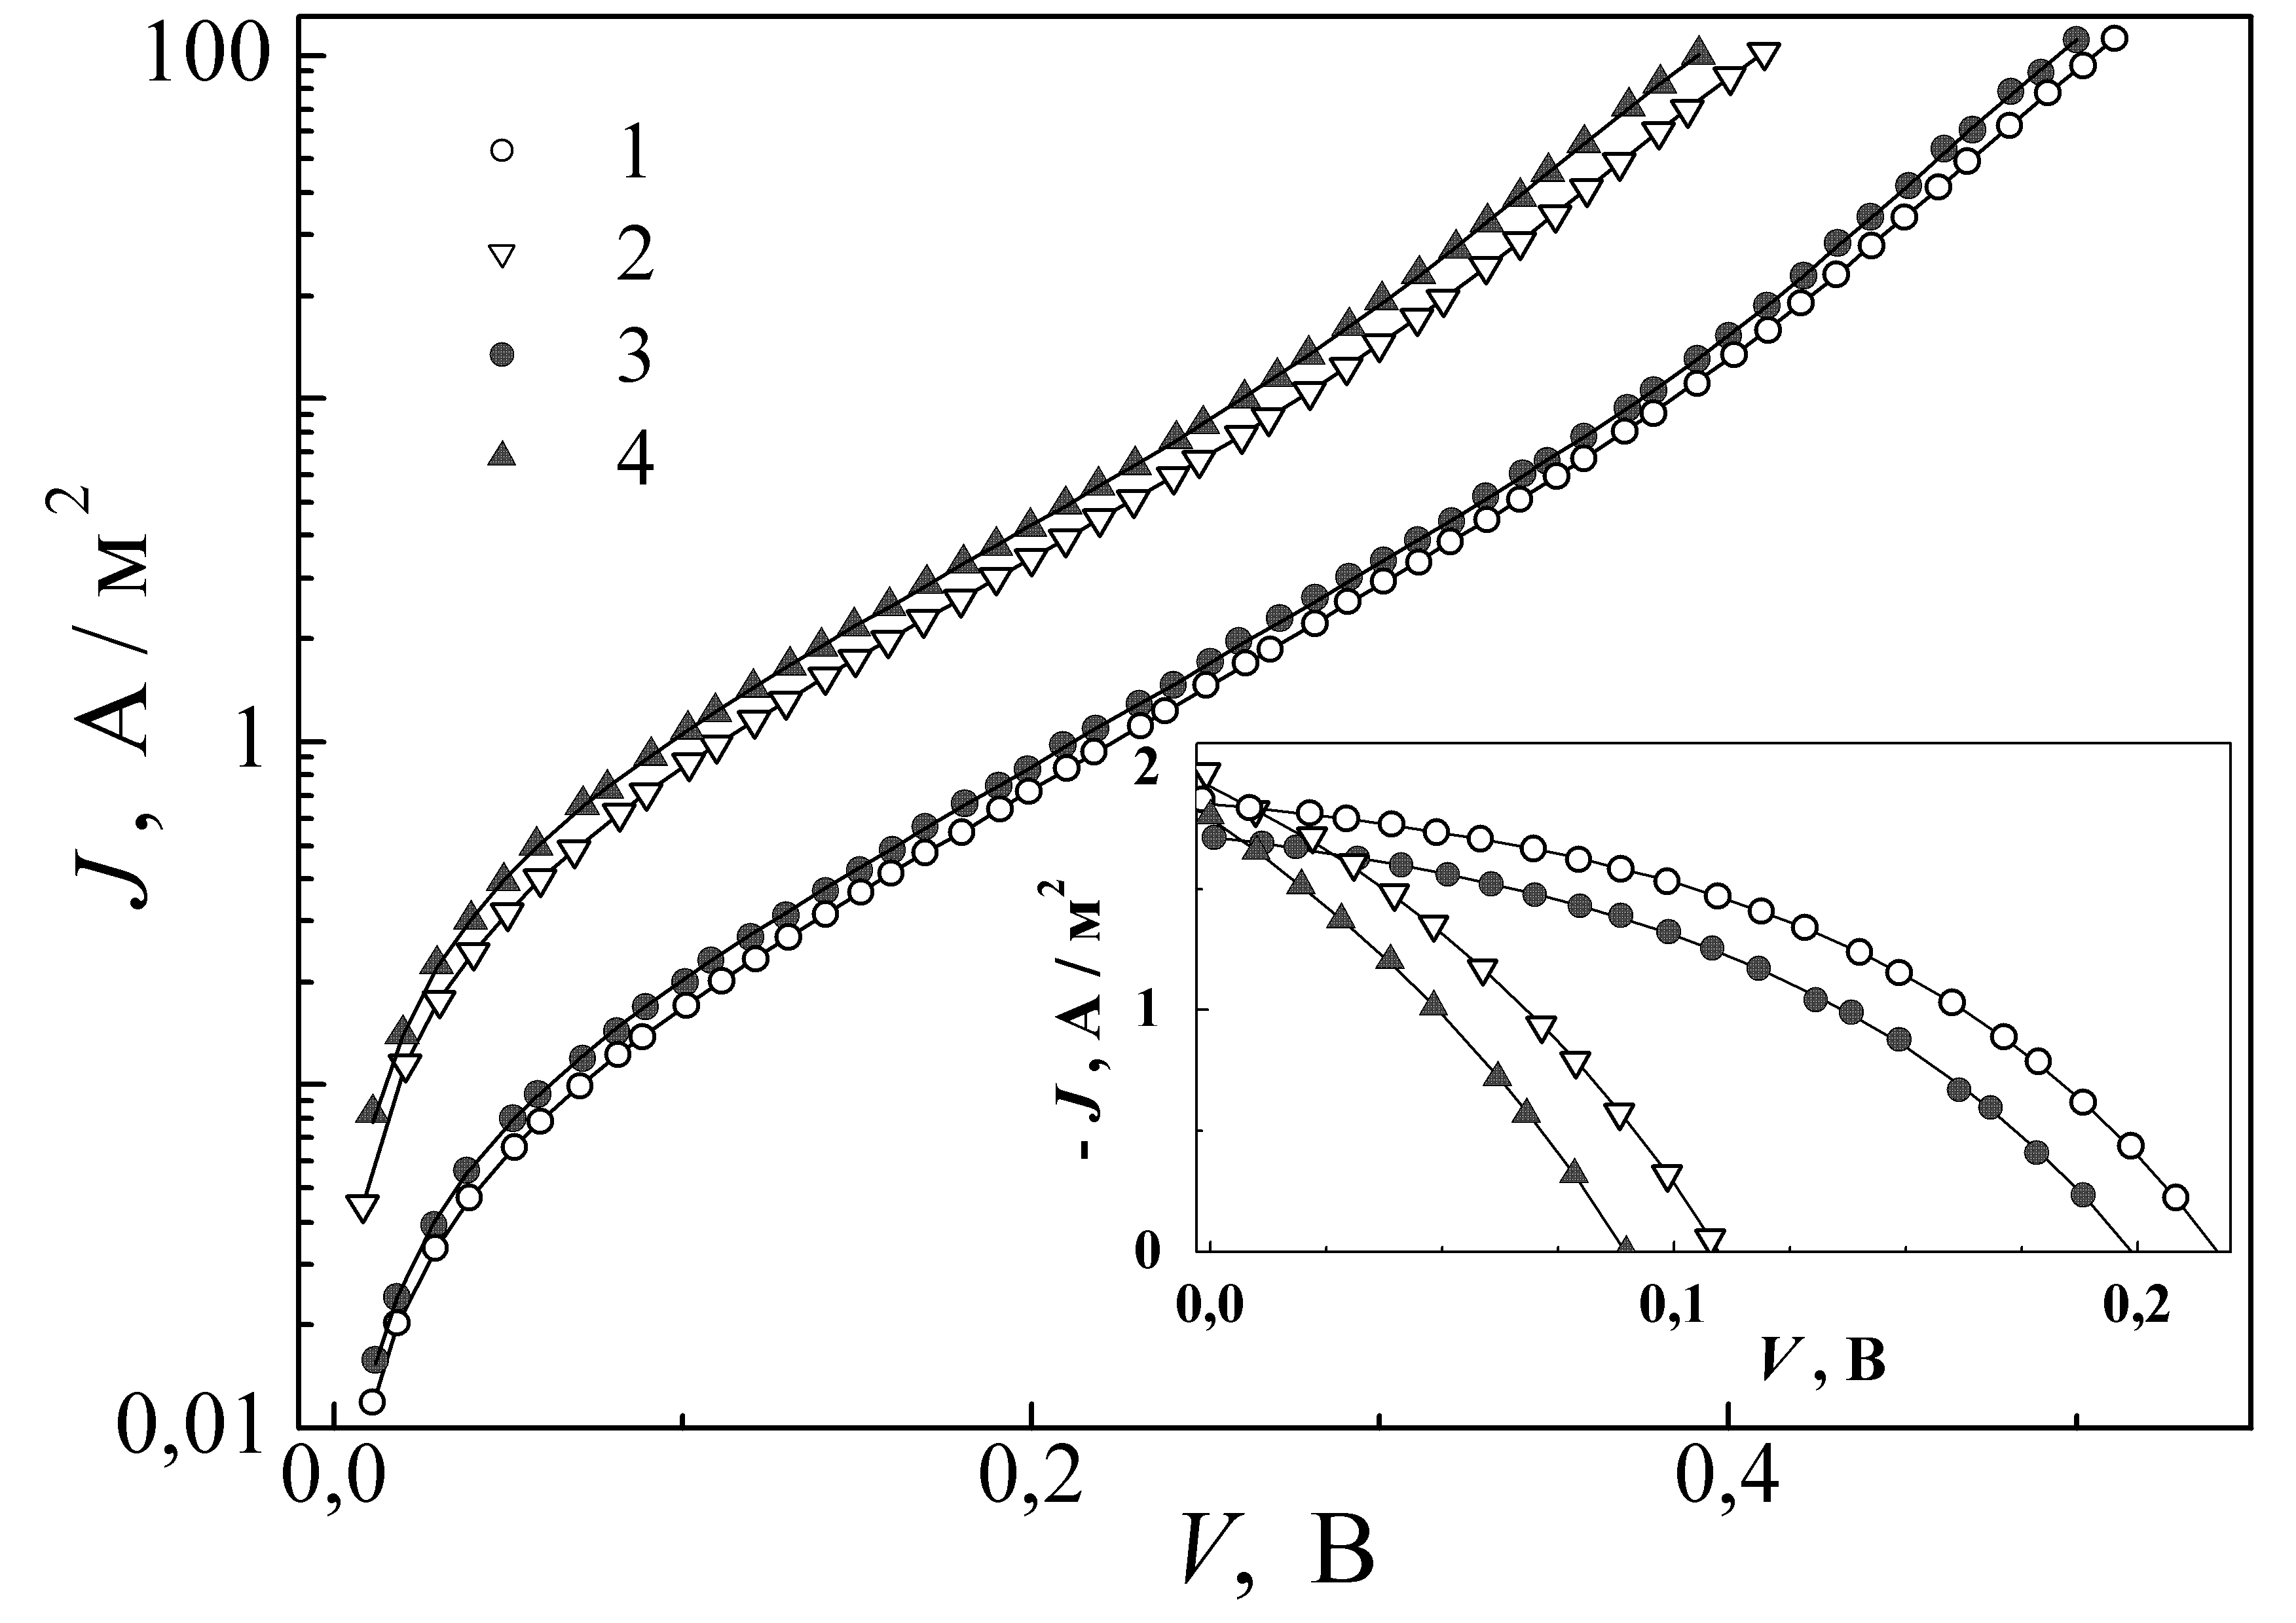
\includegraphics[width=0.9\textwidth]{figSSCIV}%
\caption{\label{figSSCIV}
Темнові ВАХ, виміряні при температурах 301~K (криві 1 та 2, кола) та 341~K (криві 2 та 4, трикутники)
за умов УЗН (U--Tb3, криві 2, 4, заповнені точки) та для ненавантаженого зразка (криві 1 та 3, порожні точки)
На вставці наведено частину ВАХ при освітлені в діапазоні прямих зміщень від 0 до $V_{oc}$.
Точки відображають результати вимірів, лінії отримані шляхом апроксимації за формулами (\ref{eqSSCIV}) та (\ref{eqW}).
%(\labelcref{eqSSCIV,eqW}) \ref{eqW}.
}%
\end{figure}

Густина струму короткого замикання $J_{sc}$, напруга холостого ходу $V_{oc}$ та фактор форми $F\!F$ визначалися з ВАХ, отриманих при освітленні,
традиційним способом за перетином експериментальної кривої з координатними осями  та по розташуванню максимуму потужності.

В рамках моделі подвійного діоду залежність густини струму $J$ від прикладеної напруги $V$ для  n$^+$--p сонячного елементу має описуватися
наступним виразом \cite{2Diod:Ishaque,2Diod:Buhler}:

\begin{eqnarray}
\label{eqSSCIV}
\nonumber J(V,\,T)&=&\left(I_{SCR}+I_{base}+I_{sh}\right)/A=\\
\nonumber &=&-J_{ph}+\frac{qn_id}{2\tau_{g}}\left\{\exp \left[\frac{q(V-JR_s)}{n_\mathrm{id}kT}\right]-1\right\}+\\
&&+\frac{qn_i^2}{p_p}\sqrt{\frac{\mu_nkT}{\tau_n}}\left\{\exp \left[\frac{q(V-JR_s)}{kT}\right]-1\right\}+\frac{V-JR_s}{R_{sh}}\,,
\end{eqnarray}
де
$I_{SCR}$ описує загальну рекомбінацію в області просторового заряду (ОПЗ)
$I_{base}$ пов'язане з процесами рекомбінації у квазі--нейтральній області (КНО),
$I_{sh}$ --- шунтуючий струм,
$A$ --- площа діоду,
$T$ --- абсолютна температура,
$J_{ph}$ --- густина фотогенерованого струму,
$q$ --- елементарний заряд,
$n_i$ --- концентрація власних носіїв заряду,
$\tau_{g}$  --- ефективний час життя носіїв заряду в ОПЗ,
$d$ --- товщина ОПЗ:
\begin{equation}
\label{eqW}
    d(V,\,T)=\sqrt{\frac{2 \varepsilon \varepsilon_0(p_p+n_n)}{q p_p n_n}\left[\frac{E_g}{q}-\frac{kT}{q}\ln\left(\frac{N_vN_c}{p_pn_n}\right)-\frac{2kT}{q}-V\right]} \,,
\end{equation}
$\varepsilon_0$ --- діелектрична стала,
$\varepsilon$ --- діелектрична проникність матеріалу (для Si $\varepsilon=11,7$),
$p_p$ та $n_n$ --- концентрація основних носіїв заряду в $p$-- та $n$--області, відповідно;
$E_g$ --- ширина забороненої зони напівпровідника,
$N_c$ та $N_v$ --- ефективна густина станів поблизу дна зони провідності та вершини валентної зони, відповідно;
$n_\mathrm{id}$ --- фактор неідеальності
$R_s$ та $R_{sh}$ --- послідовний та шунтуючий опори, відповідно;
$\mu_n$ та $\tau_n$ --- рухливість та час життя електронів (неосновних носіїв) в базі діоду.
Тобто,
рівняння ВАХ, яке моделює поведінку сонячного елементу за допомогою еквівалентної електричної схеми,
містить ряд параметрів, що безпосередньо стосуються фізичних процесів, які відбуваються у пристрої.
%Зокрема вважається, що
%$J_{0base}=(qn_i^2/n_n)\sqrt{\mu_nkT/\tau_n}$ пов'язане з процесами рекомбінації у квазі--нейтральній області (КНО), тоді як
%$J_{0SCR}=(qdn_i/2\tau_{g})$ описує загальну рекомбінацію в ОПЗ.

Формули (\ref{eqSSCIV})--(\ref{eqW}) були використані для апроксимації експериментальних даних, причому
невідомими величинами вважалися $\tau_g$, $\tau_n$, $n_{\mathrm{id}}$, $R_{sh}$, $R_s$ та  $J_{ph}$ (остання лише для ВАХ при освітленні).
При цьому вважалося, що
$n_i(T)=1,64\cdot10^{15}\,T^{1,706}\exp(-E_g/2kT)$~см$^{-3}$ \cite{ni:Green}, $N_c(T)=2,86\cdot10^{19}(T/300)^{1,58}$~см$^{-3}$, $N_v(T)=3,10\cdot10^{19}(T/300)^{1,85}$~см$^{-3}$
\cite{Nc:Green},
а температурні залежності забороненої зони та рухливості електронів описуються формулами Varshni та Caughey--Thomas, відповідно:
\begin{equation}
\label{eqEg}
 E_g(T) = E_g(0) - \frac{\beta_1 T^2}{(T + \beta_2)}\,,
\end{equation}
де
$E_g(0)=1,169$~еВ,
$\beta_1=7,021\cdot10^{-4}$~еВ/К$^2$,
$\beta_2=1108$~K \cite{Schroder2006,Markvart} та
\begin{equation}
\label{eqMu}
\mu_n(T) = \mu_{min}+\frac{\mu_0}{1+(p_p/N_{ref})^{\zeta}}\,.
\end{equation}
де
$\mu_{min}=92\cdot(T/300)^{-0,57}$~см$^2$/(В$\cdot$с),
$\mu_0=1268\cdot(T/300)^{-2,33}$~см$^2$/(В$\cdot$с),
$N_{ref}=1,3\cdot10^{17}\cdot(T/300)^{2,4}$~см$^{-3}$,
$\zeta=0,91\cdot(T/300)^{-0,146}$ \cite[с.~505, Table~A8.2]{Schroder2006}.
Апроксимація проводилась з використанням методу диференційної еволюції\cite{DE:Sun,DEWang,DEModif}, який більш детально описано в параграфі~\ref{subEA}.
Приклади результуючих апроксимуючих кривих наведено  на Рис.~\ref{figSSCIV}.
Видно, що вони досить добре апроксимують експериментальні дані.

Відомо \cite{2Diod:Buhler}, що $J_{sc}\approx J_{ph}R_{sh}/(R_{sh}+R_{s})$.
Для всіх досліджених зразків $R_s\approx1,5$~Ом$\cdot$см$^2$,
що збігається з типовим значенням $0,5\div2$~Ом$\cdot$см$^2$ \cite{Breitenstein2013,SCRs:Mette} для КСЕ.
Величина $R_{sh}$ суттєво залежала від температури та конкретного зразка, проте для
розглянутого температурного інтервалу не було меншим  4~кОм$\cdot$см$^2$.
Отже, очікується, що в нашому випадку має бути $J_{sc}\approx J_{ph}$.
І дійсно, подібне співвідношення спостерігається між величиною $J_{ph}$, отриманою шляхом багатопараметричної апроксимації
повної залежності густини струму від напруги, та значенням $J_{sc}$, яке відображає ординату перетину ВАХ з віссю струмів.

Для освітлення КСЕ використовувалося монохроматичне (довжина хвилі $\lambda=900$~нм) світло з низькою інтенсивністю.
Відомо, що освітлення з інтенсивністю $W_{ph}$ більше 5~Вт/см$^2$ викликає дисоціацію пар залізо--бор \cite{LID:CuII},
а при $W_{ph}>0.01$~suns (1~sun$=1000$~Вт/м$^2$) в кремнії р--типу утворення дефектів можуть утворюватись дефекти \cite{BO:Halam2016}.
Ці процеси впливають на час життя носіїв заряду, а так як метою роботи було дослідження АІ ефектів,
то з метою запобігання будь--яких світло--індукованих деградаційних процесів було використане
освітлення з інтенсивністю $W_{ph}=(8\pm4)$~Вт/м$^2$.
Монохроматичність світла дозволила спростити аналіз причин АІ змін струму короткого замикання.
А саме, для використаної довжини хвилі фотогенерований струм пов'язаний, переважно, з утворенням електронно--діркових пар в $p$--області.
У випадку, якщо база СКЕ перевищує у декілька разів довжину дифузії неосновних носіїв $L_n=\sqrt{\mu_nkT\tau_n/q}$, то
для $J_{sc}$ справедливий вираз \cite{Markvart,Razeghi,Faren}:
\begin{equation}
\label{eqIph}
J_{sc} = \frac{W_{ph}(1-R_{ph})q\beta\lambda}{hc}\frac{\alpha L_n}{1+ \alpha L_n}\,,
\end{equation}
де
$\alpha$ --- коефіцієнт поглинання світла,
$R_{ph}$ --- коефіцієнт відбивання,
$\beta$ --- коефіцієнт квантового виходу.

Формулу~(\ref{eqIph}) було використано для апроксимації експериментальної залежності $J_{sc}(T)$,
при чому $L_n$ розглядалась як невідомий параметр.
Під час розрахунків вважалося, що $R_{ph}$ та $\beta$ не змінюються (згідно з \cite{Gaman}, для кремнію
при використаній довжині хвилі $\beta=1$),
а температурна залежність $\alpha$ описується виразом \cite{Markvart,Si:Absorb}
\begin{eqnarray}
\label{eqAlpha}
\nonumber \alpha(\lambda,\,T)&=&\sum_{\substack{i=1,2\\j=1,2}}\!C_iA_j\left\{\frac{[hc/\lambda-E_{gj}(T)+E_{p\,i}]^2}{\exp(E_{p\,i}/kT)-1}\:+
\frac{[hc/\lambda-E_{gj}(T)-E_{p\,i}]^2}{1-\exp(-E_{p\,i}/kT)}\right\}+\\
&&+A_d\left[hc/\lambda-E_{gd}(T)\right]^{1/2}\,,
\end{eqnarray}
де
$h$ --- стала Планка,
$c$ --- швидкість світла,
$E_{p\,1}=1,827\cdot10^{-2}$~еВ,
$E_{p\,2}=5,773\cdot10^{-2}$~еВ --- частоти Дебая поперечних
оптичних та акустичних фононів, відповідно;
константи $C_1=5,5$,
$C_2=4,0$,
$A_1=3,231\cdot10^2$~см$^{-1}$еВ$^{-2}$,
$A_2=7,237\cdot10^3$ см$^{-1}$еВ$^{-2}$,
$A_d=1,052\cdot10^6$ см$^{-1}$еВ$^{-2}$;
температурна залежність $E_{g1}$, $E_{g2}$ та $E_{gd}$ описується виразом \ref{eqEg}),
причому $E_{g1}(0)=1,169$~еВ, $E_{g2}(0)=2,5$~еВ та $E_{gd}(0)=3,2$~еВ.
Крім того, припускалося що $L_n\sim T^{0.5}$.
Основою для цього були результати, отримані при апроксимації окремих ВАХ (детальніше див. параграф~\ref{sbQNR}).

Таким чином, визначення $L_n$ та $\tau_n$ проводилось як в результаті аналізу окремої ВАХ, так і з апроксимації
температурної залежності $J_{sc}$.
Надалі, щоб відрізнити величини, отримані другим шляхом, використовується верхній індекс <<$ph$>>: $L_n^{ph}$, $\tau_n^{ph}$, $\varepsilon_{\tau n}^{ph}$ тощо.

Ще раз підкреслимо, що всі АІ ефекти, описані у цьому розділі є оборотними.
Тобто, величини $J_{sc}$, $V_{oc}$, $F\!F$ та інших параметрів повертаються до своїх вихідних значень
після припинення УЗН  та витримки зразків при кімнатній температурі протягом доби.
Оборотність АІ ефектів ілюструє Рис.~\ref{figReverse}.
Часовий інтервал між початком УЗН та вимірами, результати яких представлені з позначкою <<під час УЗН>>
перевищує 60~хв, проміжок часу між закінченням УЗН та вимірами <<після УЗН>> --- близько 24~год.
На рисунку представлені дані лише для двох зразків, але ці результати є типовими і для інших.
Оборотність ефектів, зокрема, свідчить про те, що УЗ не спричинює ні дифузію дефектів,
ні зміну їх концентрації.

\begin{figure}
\center
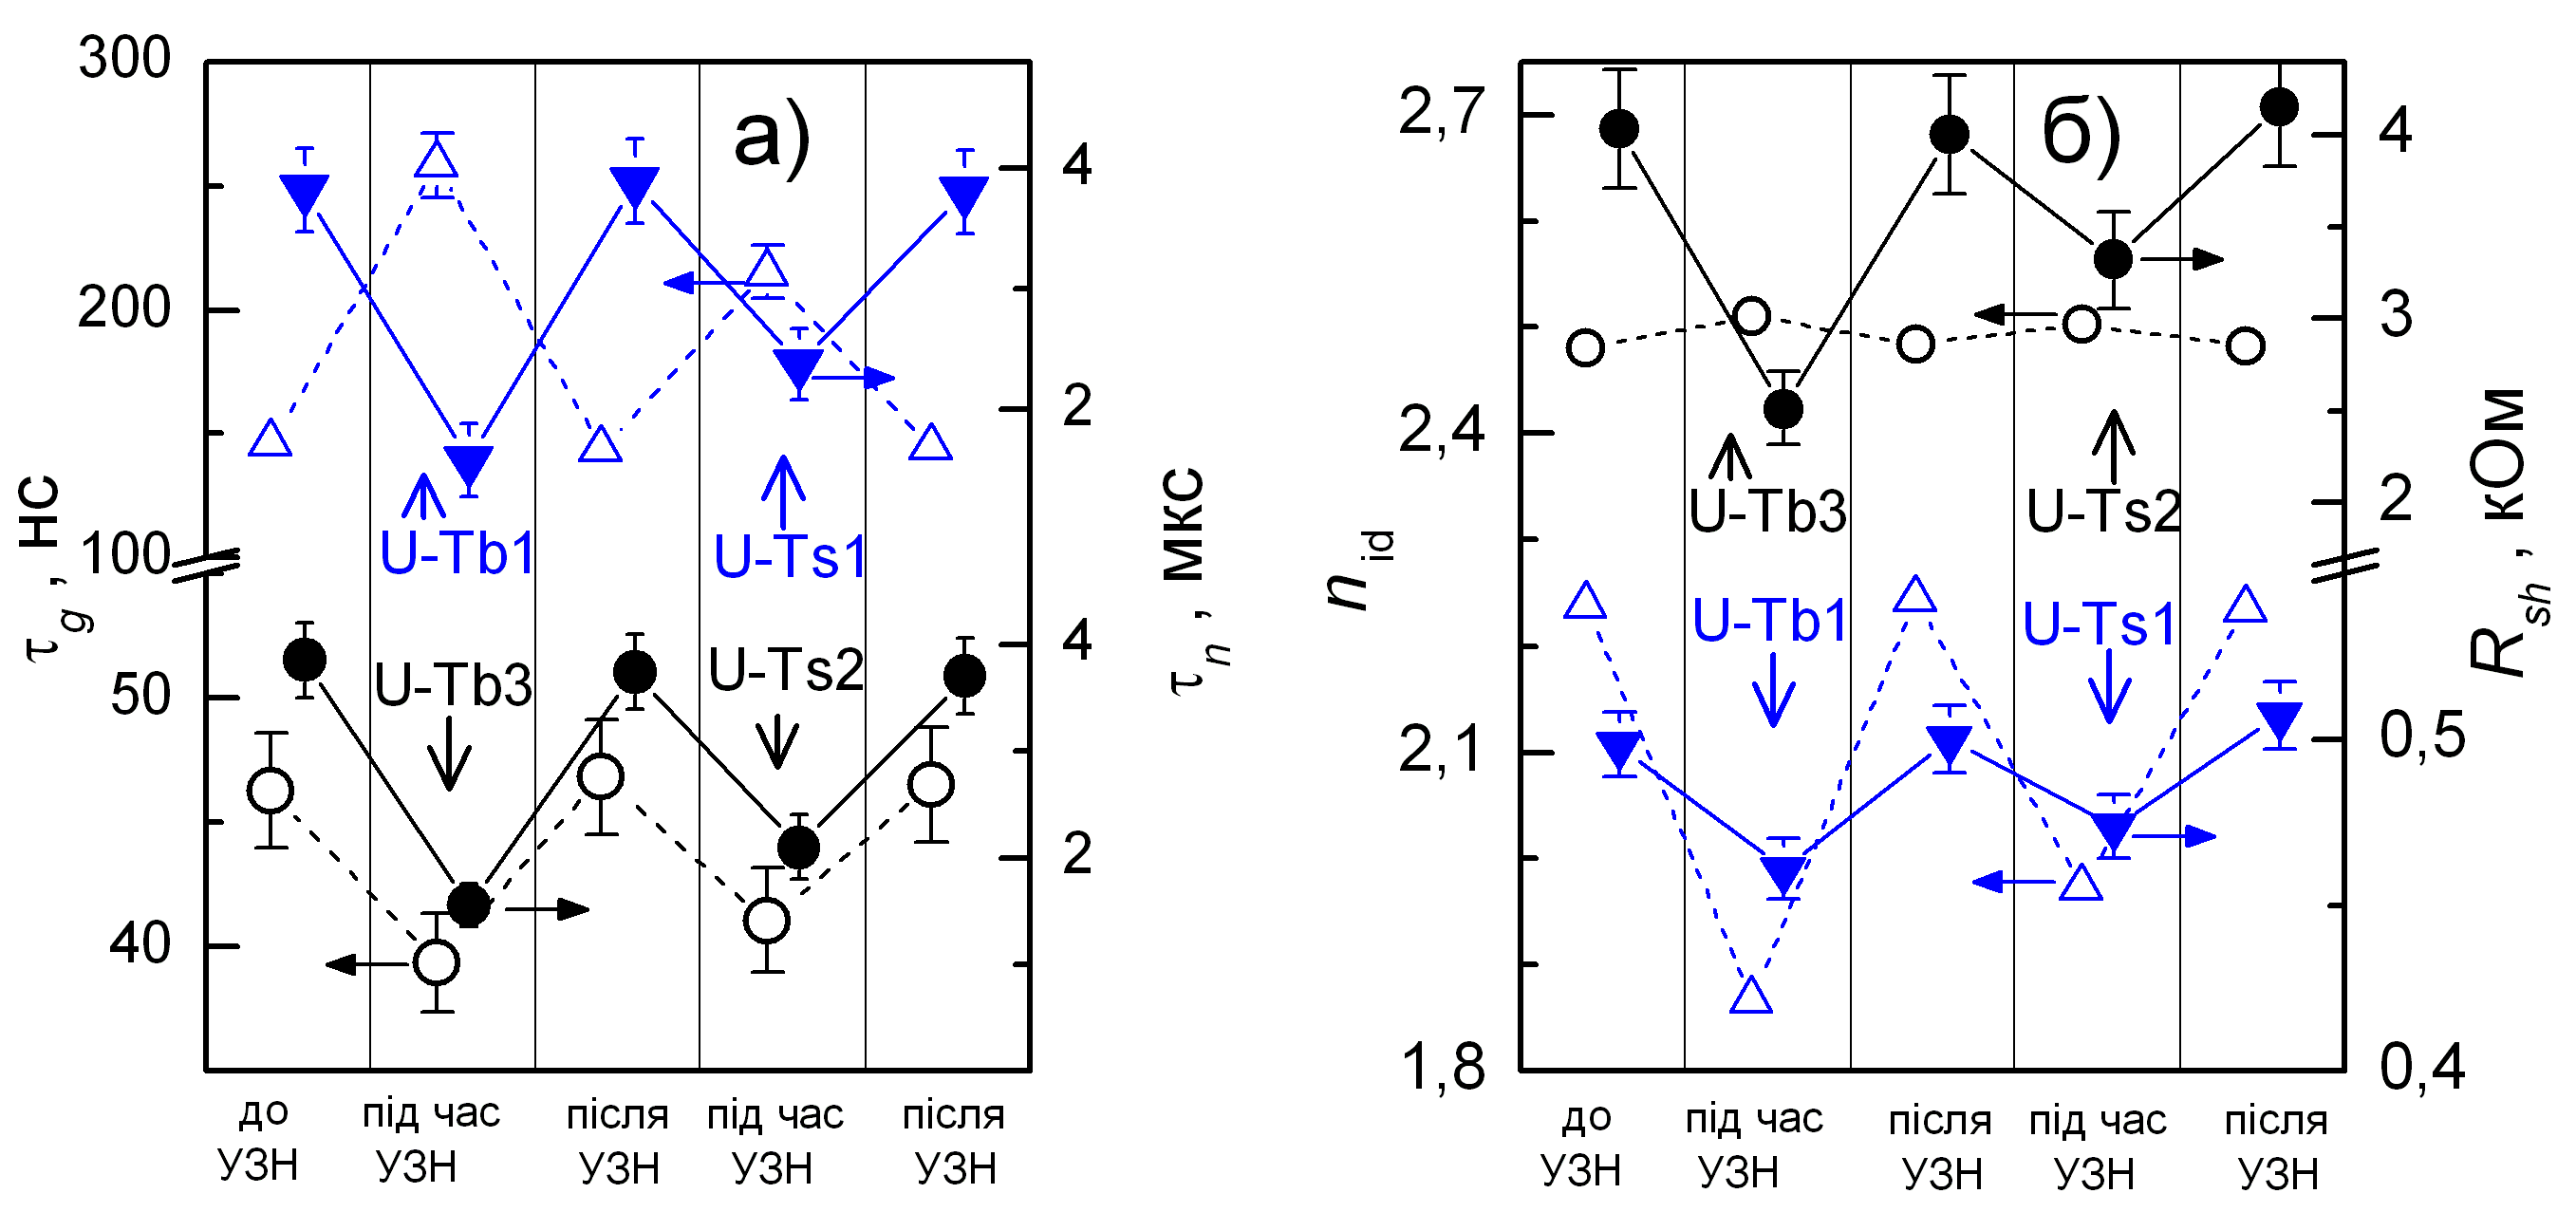
\includegraphics[width=0.85\textwidth]{figReverse}%
\caption{\label{figReverse}
Значення часу життя в ОПЗ (a, ліва вісь, незаповнені точки)
та КНО (a, права вісь, заповнені точки),
фактору неідеальності (б, ліва вісь, незаповнені точки) та
шунтуючого опору (б, права вісь, заповнені точки),
отримані до, під час та після УЗН при температурі 330~K.
Представлені дані для зразків SC11 (кола) та g7SC12 (трикутники).
}%
\end{figure}

Загалом такі параметри дво--діодної моделі як $\tau_g$, $n_{\mathrm{id}}$, $R_{sh}$ та $R_s$ можуть залежати від освітлення \cite{Iph:KHAN2010,Breitenstein2013,SUGIANTO2009}.
Наприклад, шунтуючий опір при освітленні, може бути або більшим за величину, отримане з темнових ВАХ\cite{Iph:KHAN2010}, або меншим \cite{Breitenstein2013,SUGIANTO2009}.
В літературі \cite{Breitenstein2013} подібний ефект пов'язують з відхиленням від принципу суперпозиції,
згідно з яким струм, що протікає через КСЕ при освітленні, має дорівнювати сумі темнового струму за тих же умов та фотогенерованого струму ($I_{ph}$).
В свою чергу, відхилення можуть бути пов'язані з насиченням рекомбінації за участю дефектів,
збуренням концентрації носіїв у збідненому шарі внаслідок протікання фотоструму \cite{Robinson} або з впливом послідовного опору \cite{Rs:BREITENSTEIN2013}.
Проте відмінності параметрів стають суттєвими, коли інтенсивність освітлення перевищує 0,1~sun \cite{Breitenstein2013}.
В нашому випадку темнові ВАХ та світлові, зміщені на величину струму короткого замикання, практично збігаються (Рис.~\ref{figIVIscVoc}),
як і величини $\tau_g$, $\tau_n$, $n_{\mathrm{id}}$, $R_{sh}$ та $R_s$, отримані з ВАХ, які виміряні у темряві та при освітленні за однакової температури
та в ідентичних умовах УЗН.
На рисунку також наведена залежність струму короткого замикання від напруги холостого ходу, отримана при різних значеннях $W_{ph}$.
Те, що вона співпадає з темновою ВАХ свідчить про малий вплив послідовного опору \cite{Robinson}.

\begin{figure}
\center
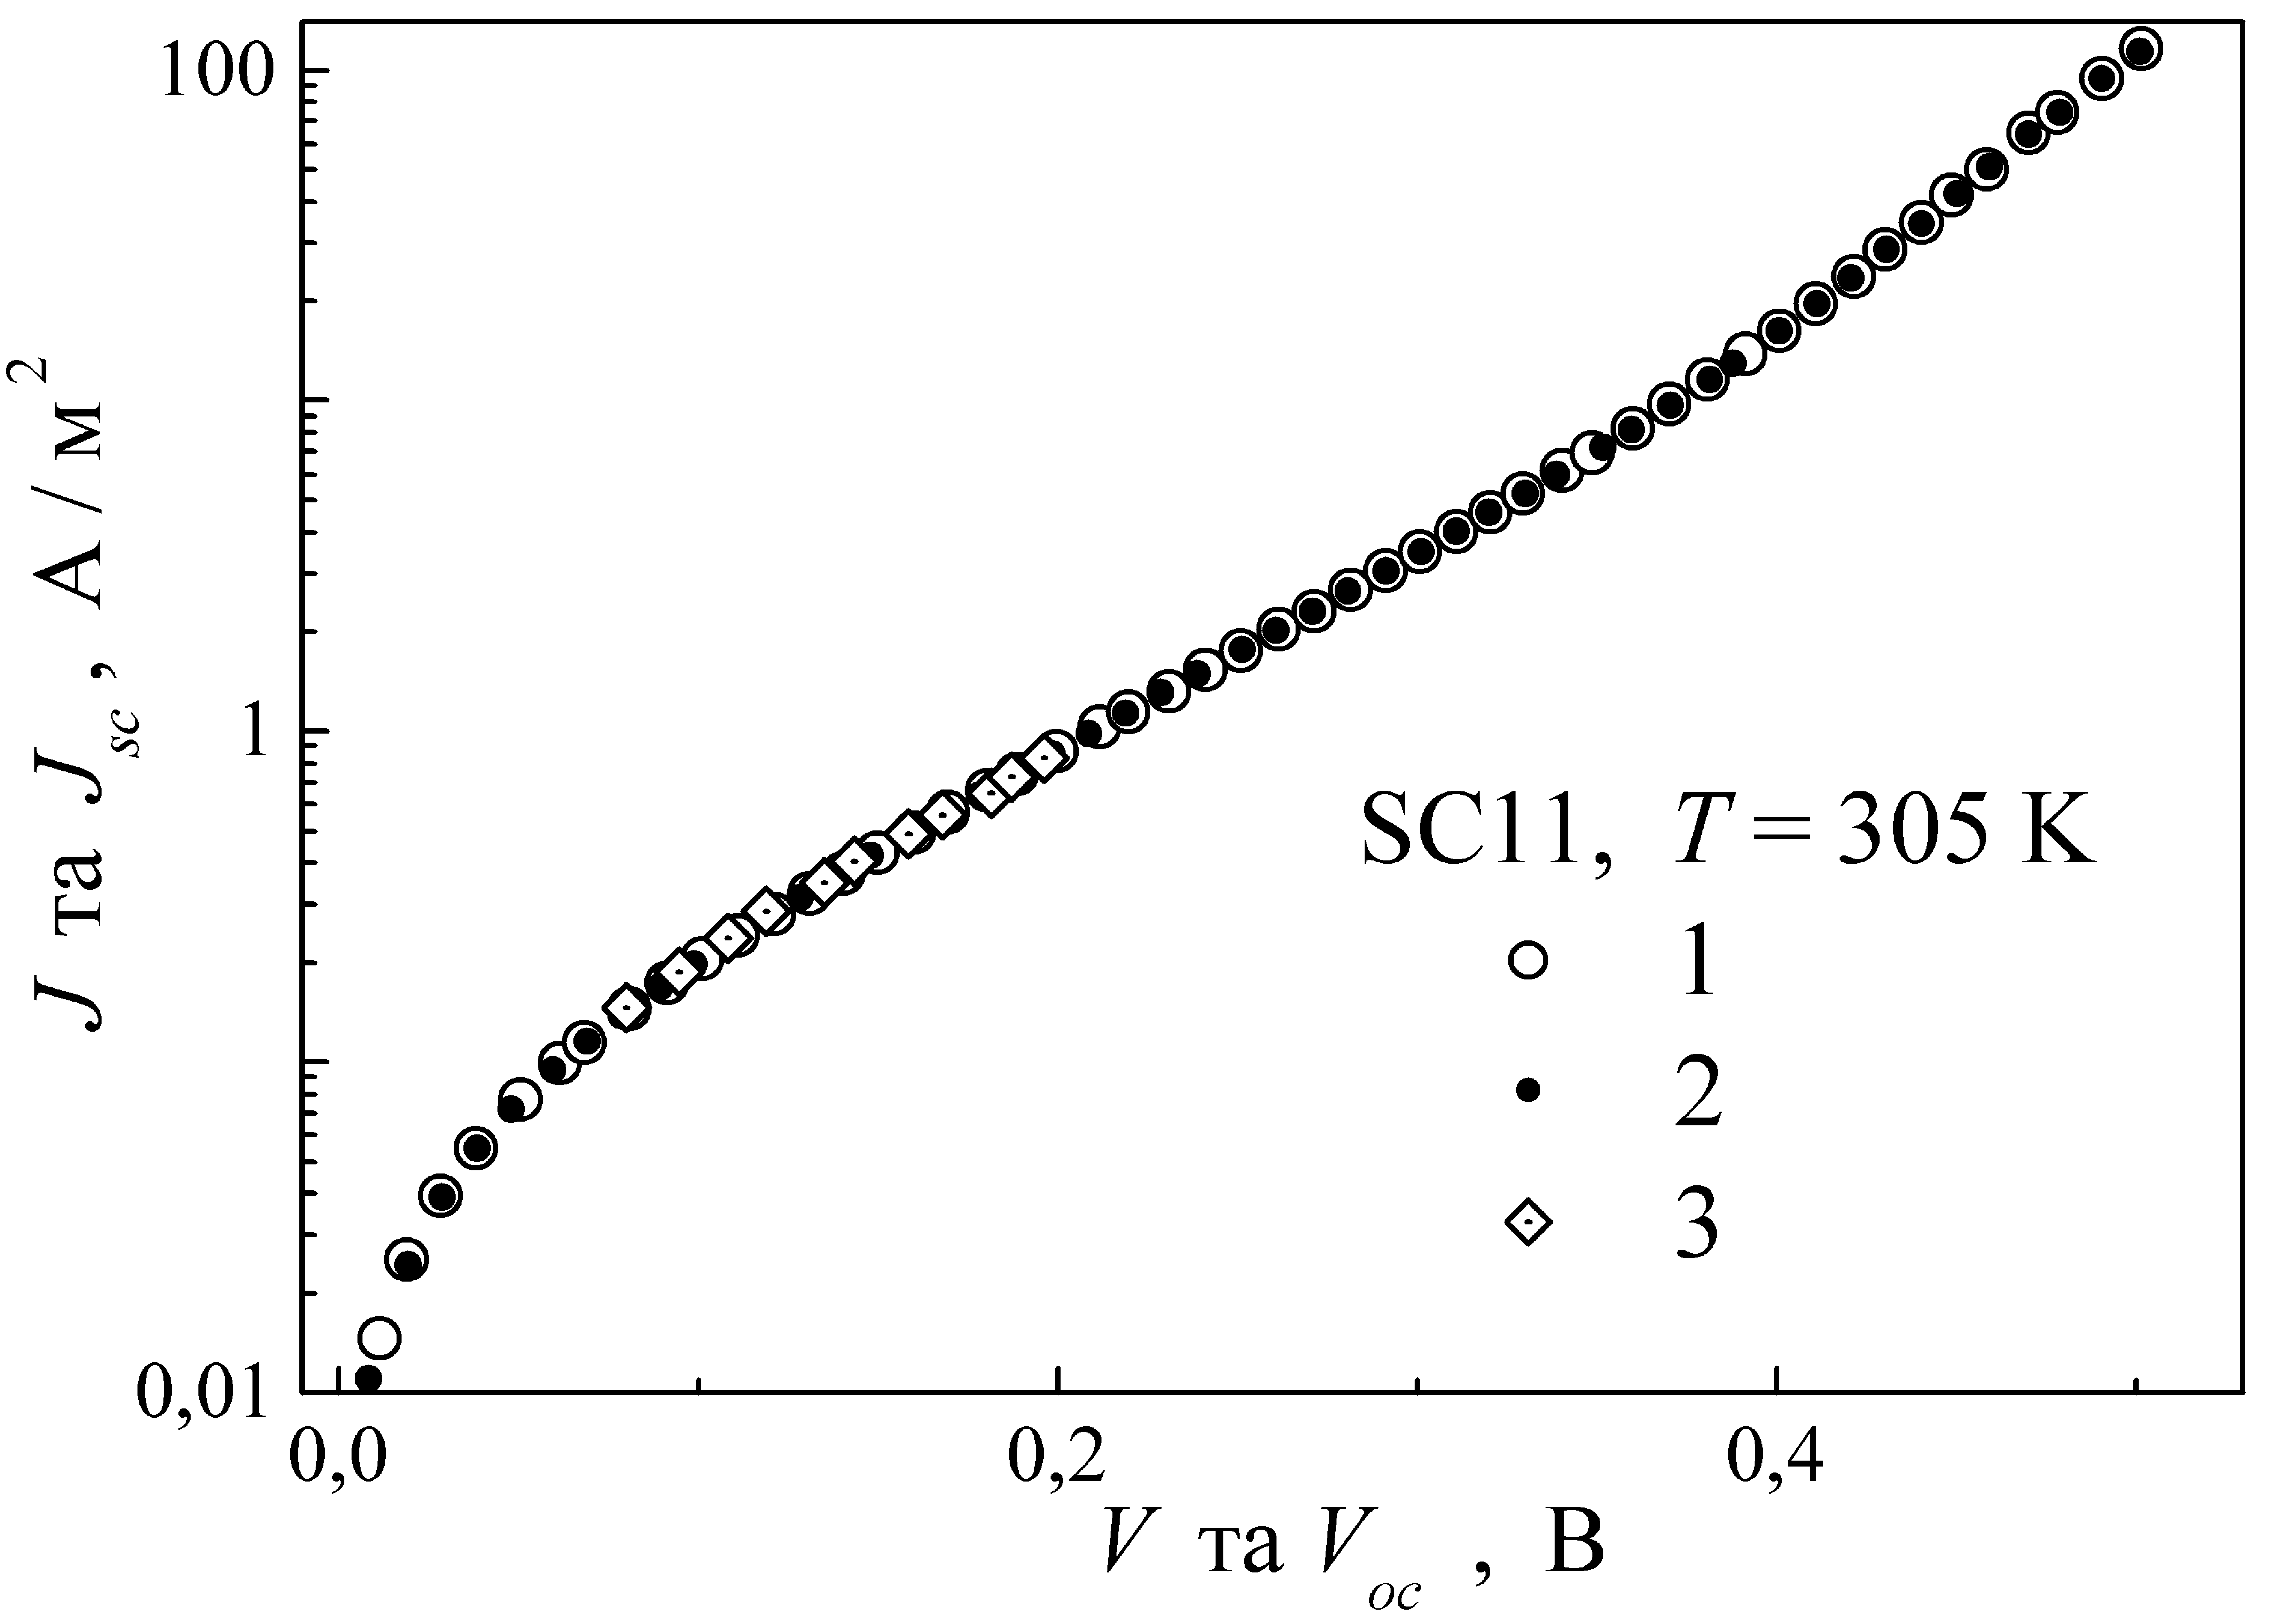
\includegraphics[width=0.5\textwidth]{figIVIscVoc}%
\caption{\label{figIVIscVoc}
Темнова ВАХ (1),
світлова ВАХ, зміщена на величину струму короткого замикання (2)
та залежність $I_{sc}-V_{oc}$ (3).
Зразок SC11.
$T=305$~К.
}%
\end{figure}

Відомо, що дефекти розподіляються по площі напівпровідникових пластин нерівномірно (див., наприклад, \cite{Oxide:Chen,Oxide_Schon}),
а отже, нерівномірним є і розподіл фізичних параметрів.
В нашому випадку також спостерігався розкид величин визначених параметрів зразків, вирізаних з різних частин вихідної пластини (див. Рис.~\ref{figSSC},б).
Проте характер АІ змін цих параметрів для всіх зразків був подібний.
Тому з усього набору досліджених структур (5 зразків) надалі в цьому параграфі представлено типові результати переважно лише для двох (SC11 та SC17),
вихідні параметри яких відрізнялися найбільше.



\subsection{Вплив ультразвукового навантаження на фотоелектричне перетворення в КСЕ}

Отримані температурні залежності густини струму короткого замикання, напруги холостого ходу та фактору форми наведено на Рис.~\ref{figDUSIsc}.
Значення параметрів при температурі 320~K представлені в Таблиці~\ref{tabSSCParam}.
Необхідно зауважити, що не тільки $J_{sc}$ та $V_{oc}$, але й коефіцієнт корисної дії, $F\!F$ та час життя неосновних носіїв
заряду зменшуються за умов освітлення з низькою інтенсивністю\cite{LI:Ruhle,LI:Reich,LI:lifetime}.
Зокрема, збільшення часу життя неосновних носіїв при зростанні їх концентрації може спостерігатися
а)~за наявності точкових рекомбінаційних центрів з суттєво різними за величиною коефіцієнтами
захоплення носіїв різного знаку \cite{Breitenstein2013,TauOnIph};
б)~коли рекомбінація відбувається на протяжних дефектах, які здатні накопичувати
неосновні носії, що викликає появу потенційного бар'єру та зменшення коефіцієнта захоплення \cite{Robinson1995,Schroter1995}.

Таким чином, дані на Рис.~\ref{figDUSIsc} та в Таблиці~\ref{tabSSCParam} не є еквівалентними тим, що
можуть бути отримані за стандартних умов (STC, standard test condition, інтенсивність освітлення 1000~Вт/м$^2$,
температура $25^{\circ}$C, спектр AM1.5G).
Проте вони ілюструють АІ ефекти.
Крім того, середньо--річна енергетична ефективність сонячних батарей в наших широтах суттєво залежить від
їх продуктивності при низькому рівні освітлення.


%\begin{figure}[b]
\begin{figure}
\center
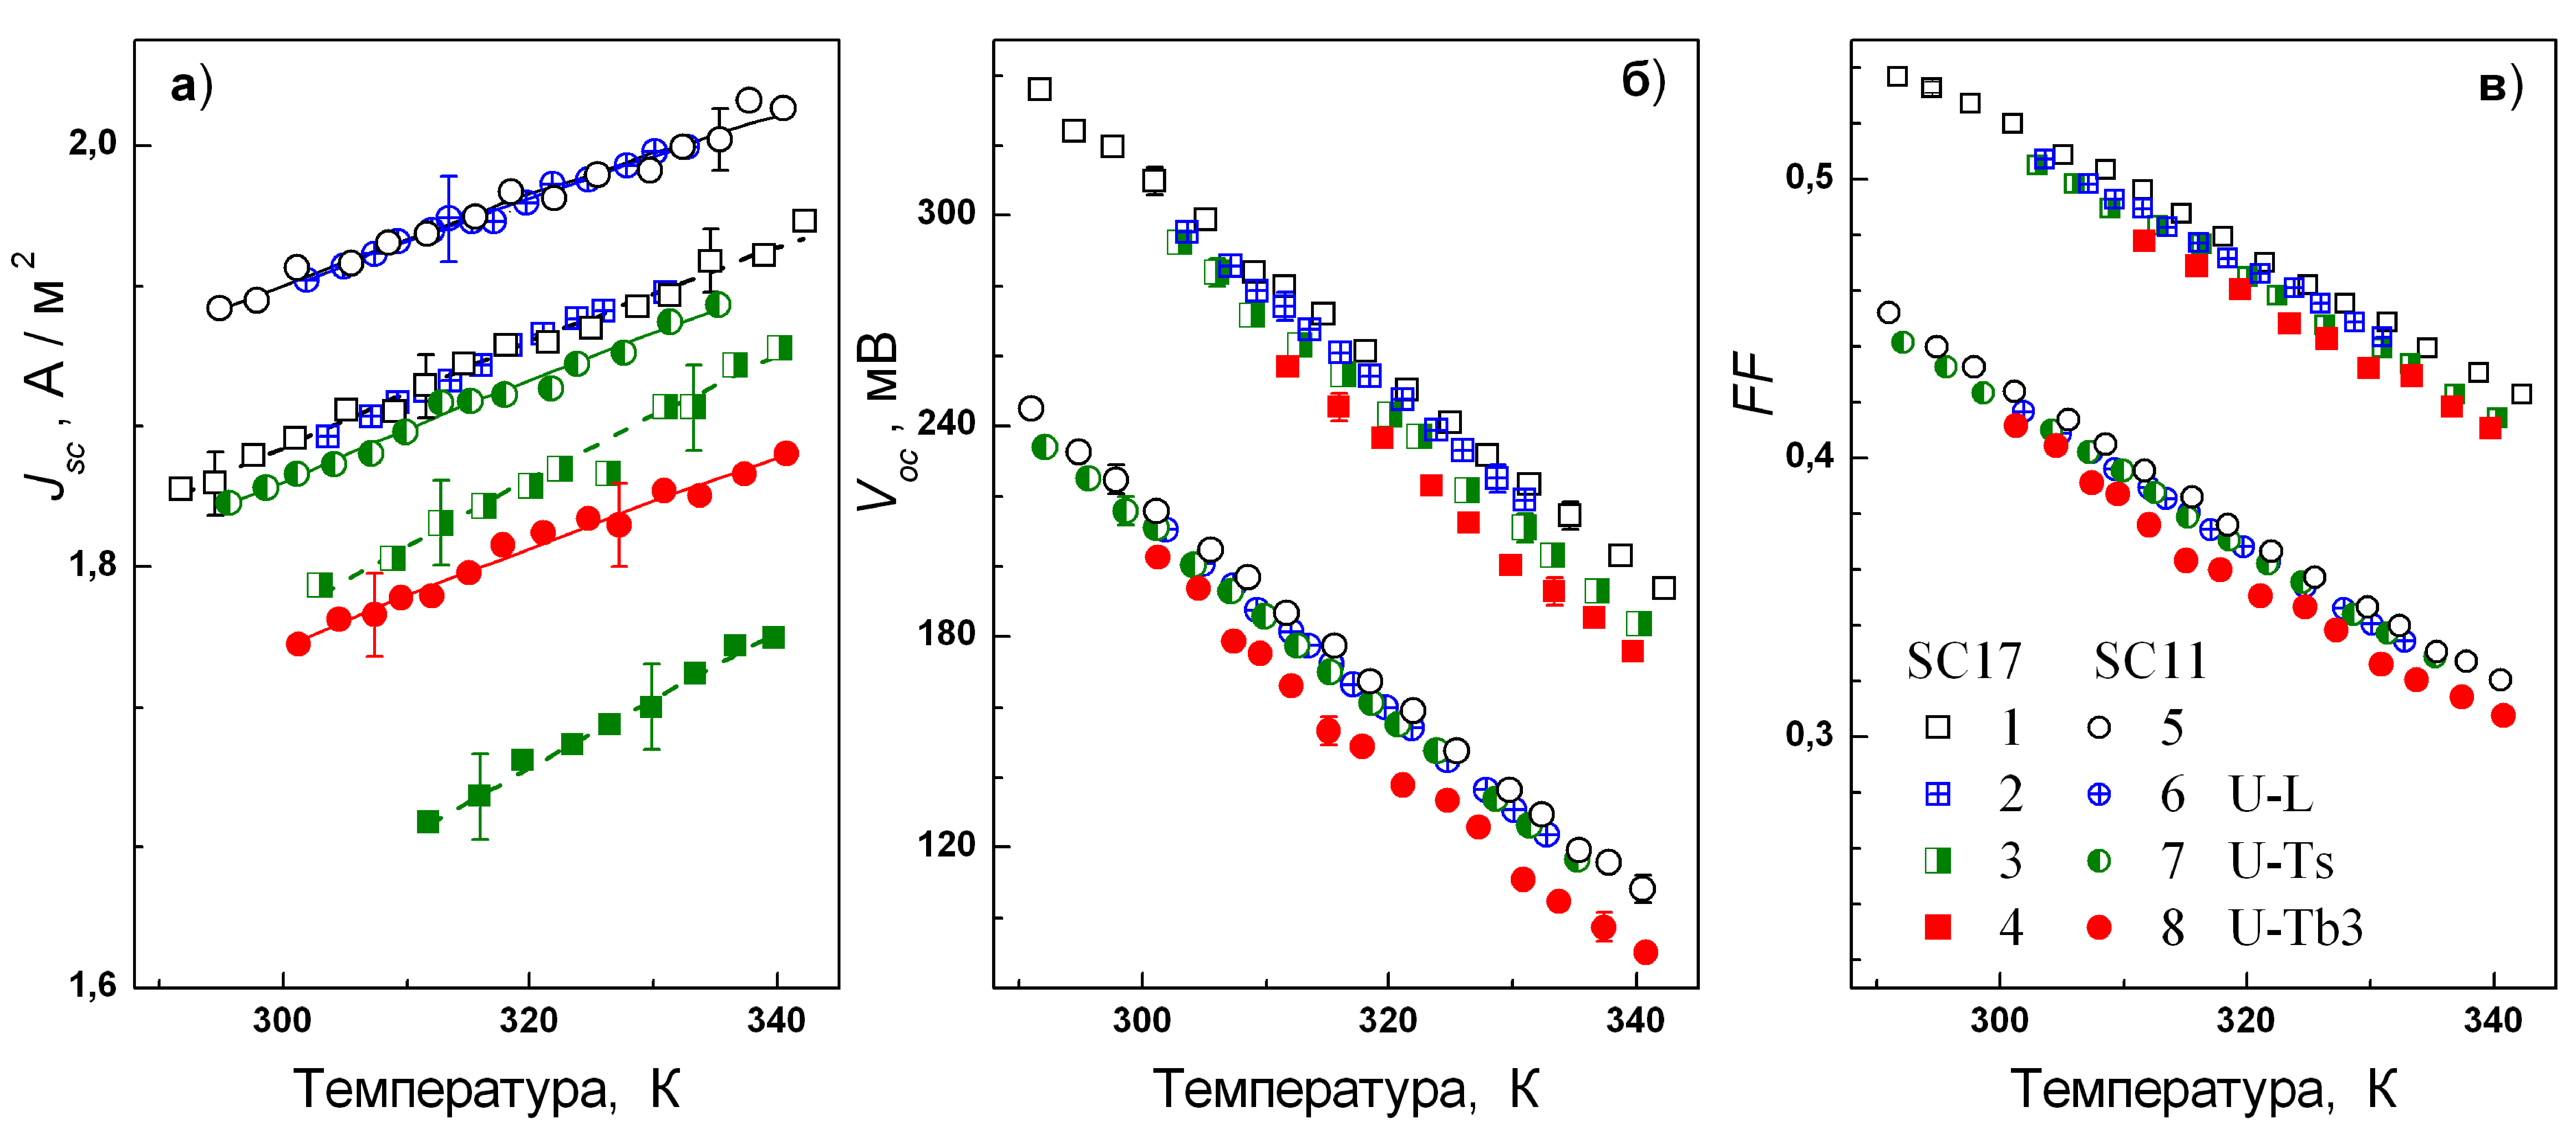
\includegraphics[width=1\textwidth]{figDUSIsc}%
\caption{\label{figDUSIsc}
Температурна залежність густини струму короткого замикання (а),
напруги холостого ходу (б) та
фактору форми (в)
для структур SC17 (квадрати) and SC11 (кола).
\FigCaptionSSC
%Криві 1 та 5 (незаповнені символи) отримані без УЗН,
%решта --- під час УЗН: U--L (криві 2 та 6),
%U--Ts1 (3),  U--Ts2 (7) та U--Tb3 (4 та 8).
Точки відповідають експериментально отриманим результатам,
лінії --- результати апроксимації згідно з формулою~(\ref{eqIph}).
}%
\end{figure}


\begin{table}
\caption{\label{tabSSCParam}Визначені параметри КСЕ ($T=320$~K).
}
\small
\begin{tabular}{|l|c|c|c|c|c|c|c|c|}
\hline
&\multicolumn{4}{c|}{SC17}&\multicolumn{4}{|c|}{SC11}\\
Параметр&\multicolumn{4}{c|}{УЗН}&\multicolumn{4}{|c|}{УЗН}\\ \cline{2-9}
&---&U--L&U--Ts1&U--Tb3&---&U--L&U--Ts2&U--Tb3\\
%\hline
\hhline{|=========|}
$J_{sc}$, 0.01A/м$^2$&191$\pm$2&191$\pm$2&184$\pm$2&171$\pm$2&198$\pm$2&198$\pm$2&189$\pm$2&181$\pm$2\\ \hline
$V_{oc}$, мВ&256$\pm$4&250$\pm$4&243$\pm$4&233$\pm$4&164$\pm$4&159$\pm$4&157$\pm$4&141$\pm$4\\ \hline
$F\!F$, $10^{-3}$&475$\pm$2&468$\pm$2&463$\pm$2&458$\pm$2&372$\pm$2&366$\pm$2&366$\pm$2&353$\pm$2\\ \hline
$L_n^{ph}$, мкм&99$\pm$5&92$\pm$5&67$\pm$4&55$\pm$3&125$\pm$6&124$\pm$6&103$\pm$5&98$\pm$5\\ \hline
$L_n$, мкм&93$\pm$5&82$\pm$4&47$\pm$3&34$\pm$2&106$\pm$5&99$\pm$5&80$\pm$4&69$\pm$4\\ \hline
$\tau_n^{ph}$, $10^{-7}$ с$^*$&31$\pm$3&26$\pm$3&14$\pm$2&9$\pm$1&49$\pm$5&48$\pm$5&33$\pm$4&30$\pm$3\\ \hline
$\tau_n$, $10^{-7}$ с&26$\pm$3&21$\pm$3&7$\pm$2&3.5$\pm$0.7&35$\pm$3&31$\pm$3&20$\pm$3&15$\pm$2\\ \hline
$\tau_g$, $10^{-9}$ с&70$\pm$4&66$\pm$3&57$\pm$3&48$\pm$2&35$\pm$2&31$\pm$2&30$\pm$2&29$\pm$2\\ \hline
$E_{\tau g}$, меВ&242$\pm$7&237$\pm$5&234$\pm$5&234$\pm$5&245$\pm$6&234$\pm$5&241$\pm$5&243$\pm$5\\ \hline
$n_\mathrm{id}$, $\pm$0.01&2.59&2.60&2.61&2.63&2.51&2.52&2.53&2.54\\ \hline
$T_\mathrm{id}$, K&226$\pm$8&215$\pm$10&243$\pm$15&233$\pm$15&327$\pm$10&319$\pm$15&308$\pm$20&358$\pm$25\\ \hline
$K_\mathtt{US}$, м$^{-2}$с$^{-1}$&\multicolumn{4}{c|}{(3.3$\pm$0.5)$\times10^{24}$}&\multicolumn{4}{|c|}{(5.0$\pm$0.2)$\times10^{23}$}\\ \hline
$R_{sh}$, кОм$\cdot$см$^2$&$>10^{12}$&$>10^{12}$&$>10^{12}$&$>10^{12}$&12$\pm$1&13$\pm$1&10$\pm$1&8$\pm$1\\ \hline
%\multicolumn{9}{l}{$^*$ determined by using the whole temperature range}
\end{tabular}
\end{table}

Так, Рис.~\ref{figDUSIsc} показує, що має місце акусто--керована деградація як струму короткого замикання, так і напруги холостого ходу та
фактора форми.
Відносні АІ зміни  параметрів наведено в Таблиці~\ref{tabAIEfect}.
Зауважимо, величина АІ змін слабко залежить від температури у розглянутому температурному діапазоні практично для всіх параметрів, які розглядались в роботі.


\begin{table}
\caption{\label{tabAIEfect}Акусто--індуковані зміни параметрів КСЕ.
}
\center
%\begin{tabular}{|c|c|c|c|c|c|c|}
\begin{tabularx}{\textwidth}{| >{\centering\arraybackslash}X|
                              >{\centering\arraybackslash}X|
                              >{\centering\arraybackslash}X|
                              >{\centering\arraybackslash}X|
                              >{\centering\arraybackslash}X|
                              >{\centering\arraybackslash}X|
                              >{\centering\arraybackslash}X|
  }
\hline
&\multicolumn{3}{c|}{SC17}&\multicolumn{3}{|c|}{SC11}\\
Параметр&\multicolumn{3}{c|}{УЗН}&\multicolumn{3}{|c|}{УЗН}\\ \cline{2-7}
&U--L&U--Ts1&U--Tb3&U--L&U--Ts2&U--Tb3\\
%\hline
\hhline{|=======|}
%&\multicolumn{3}{|c|}{SC17}&\multicolumn{3}{c|}{SC11}\\  \hline
%Параметр&U--L&U--Ts1&U--Tb3&U--L&U--Ts2&U--Tb3\\ \hline
$\varepsilon_{Jsc}$, \%&0$\pm$1&4$\pm$1&10$\pm$1&0$\pm$1&5$\pm$1&9$\pm$1\\ \hline
$\varepsilon_{Voc}$, \%&2$\pm$2&5$\pm$2&9$\pm$2&3$\pm$2&4$\pm$2&14$\pm$2\\ \hline
$\varepsilon_{F\!F}$, \%&2$\pm$1&3$\pm$1&4$\pm$1&2$\pm$1&2$\pm$1&5$\pm$1\\ \hline
$\varepsilon_{Ln}^{ph}$, \%&7$\pm$7&32$\pm$7&44$\pm$7&1$\pm$7&18$\pm$7&22$\pm$7\\ \hline
$\varepsilon_{Ln}$, \%&12$\pm$6&49$\pm$6&63$\pm$6&6$\pm$6&25$\pm$6&35$\pm$6\\ \hline
$\varepsilon_{\tau n}^{ph}$, \%&16$\pm$15&55$\pm$15&70$\pm$15&2$\pm$15&33$\pm$15&39$\pm$15\\ \hline
$\varepsilon_{\tau n}$, \%&19$\pm$12&73$\pm$12&87$\pm$12&11$\pm$12&43$\pm$12&57$\pm$12\\ \hline
$\varepsilon_{\tau g}$, \%&6$\pm$5&19$\pm$5&31$\pm$5&9$\pm$5&14$\pm$5&17$\pm$5\\ \hline
-$\Delta n_\mathrm{id}$, $10^{-2}$&1$\pm$1&2$\pm$1&4$\pm$1&1$\pm$1&2$\pm$1&3$\pm$1\\ \hline
$\varepsilon_{R sh}$, \%&&&&-8$\pm$10&17$\pm$10&33$\pm$10\\ \hline
%\end{tabular}
\end{tabularx}
\end{table}

Значення інтенсивності АХ під час УЗН U--L, U--Ts1 та U--Ts2 близькі (див. Таблицю~\ref{tabUSL}).
Проте наведені дані свідчать, що $J_{sc}$ та $V_{oc}$ більше змінюються під час U--Ts1 та U--Ts2, тобто при використанні поперечних хвиль.
В той же час, U--L та U--Ts відрізняються значеннями $f_\mathtt{US}$ та $u_\mathtt{US}$ ($\xi_\mathtt{US}$).
Проте раніше \cite{Olikh:FTP2011,Olikh:Ultras2016} було показано, що збільшенні частоти УЗН ефективність впливу ультразвуку
на кремнієві структури зростає.
Отже, ефективність УЗ дії на КСЕ визначається насамперед зміщенням атомів (деформацією ґратки),
а не інтенсивністю АХ (загальною енергією коливань, енергією яку отримує кристал під час УЗН).
З цієї точки зору поперечні АХ є більш ефективним інструментом впливу, ніж повздовжні,
так як за однакових енергетичних затрат дозволяють досягти більшого ефекту.

Рівняння (\ref{eqIph}) показує, $J_{sc}$ суттєво залежить від довжини дифузії неосновних носіїв.
Визначені шляхом апроксимації експериментальних залежностей значення $L_n^{ph}$ та розраховані на їх основі величини $\tau_n^{ph}$,
а також їх зміни в умовах УЗН наведено в Таблицях~\ref{tabSSCParam} та \ref{tabAIEfect}.
Лінії Рис.~\ref{figDUSIsc},a відображають результати апроксимації.
Отримані результати показують, що УЗ впливає на час життя неосновних носіїв і саме цим можна пояснити виявлені зміни струму короткого замикання в ультразвуковому полі.

На жаль, аналітичних виразів для $V_{oc}$ та $F\!F$ у випадку моделі подвійного діоду у літературі не запропоновано.
В той же час аналіз виразів на кшталт

\begin{eqnarray}
\label{eqSSCVoc}
 J_{sc}&=&\frac{qn_id}{2\tau_{g}}\left(e^{\frac{qV_{oc}}{n_\mathrm{id}kT}}-1\right)
+\frac{qn_i^2}{p_p}\sqrt{\frac{\mu_nkT}{\tau_n}}\left(e^{\frac{qV_{oc}}{kT}}-1\right)+\frac{V_{oc}}{R_{sh}}\,,\\
J_{sc}\left(2+\frac{R_s}{R_{sh}}\right)&=&\frac{qn_id}{2\tau_{g}}\left(e^{-\frac{qJ_{sc}R_s)}{n_\mathrm{id}kT}}-1\right)
+\frac{qn_i^2}{p_p}\sqrt{\frac{\mu_nkT}{\tau_n}}\left(e^{-\frac{qJ_{sc}R_s}{kT}}-1\right)
\end{eqnarray}
з одного боку дещо утруднений, проте з іншого показує напруга холостого ходу та фактор форми
залежать від $\tau_n$, $n_\mathrm{id}$, $\tau_g$, та $R_{sh}$.
У наступному параграфі розглянуто вплив УЗ на ці параметри.
Причини змін $V_{oc}$ та  $F\!F$ обговорені в параграфі~\ref{sbVocSim}.


\subsection{Особливості акустичного керування рекомбінацією в КСЕ\label{sbQNR}}

Традиційно, під час аналізу процесів, які відбуваються у структурах з $p-n$--переходом окремо розглядаються рекомбінацію в ОПЗ та в КНО.
Зокрема, вплив рекомбінації в ОПЗ є суттєвим для КСЕ (особливо з тиловою металізацією зокрема), які працюють в області низьких
освітленостей та при вимірах малосигнальних значень фото--ерс \cite{Sach:UPJ2016} --- тобто за умов, які відповідають нашим експериментам.


Параметрами ВАХ, які пов'язані з процесами в області просторового заряду є $n_{\mathrm{id}}$ та $J_{0SCR}=(qdn_i/2\tau_{g})$.
Під час аналізу отриманих результатів вважалося, що УЗ з невисокою інтенсивністю, використаний в роботі, не
викликає зміни параметрів напівпровідника, які визначаються основною ґраткою (тобто  $E_g$, $N_c$, $N_v$ тощо).
Тому замість розгляду величини $J_{0SCR}$ як цілого, основна увага була приділена $\tau_{g}$.
Отримані температурні залежності часу життя носіїв в ОПЗ та фактору неідеальності наведені на Рис.\ref{figDUS},a та Рис.~\ref{figDUS},б, відповідно.
Виявлено, що експериментальна температурна залежність $\tau_{g}$ цілком задовільно описується виразом
\begin{equation}
\label{eq_TAUgT}
    \tau_{g}(T)=\tau_{g0}\exp\left(-\frac{E_{\tau g}}{kT}\right)\:.
\end{equation}

\begin{figure}
\center
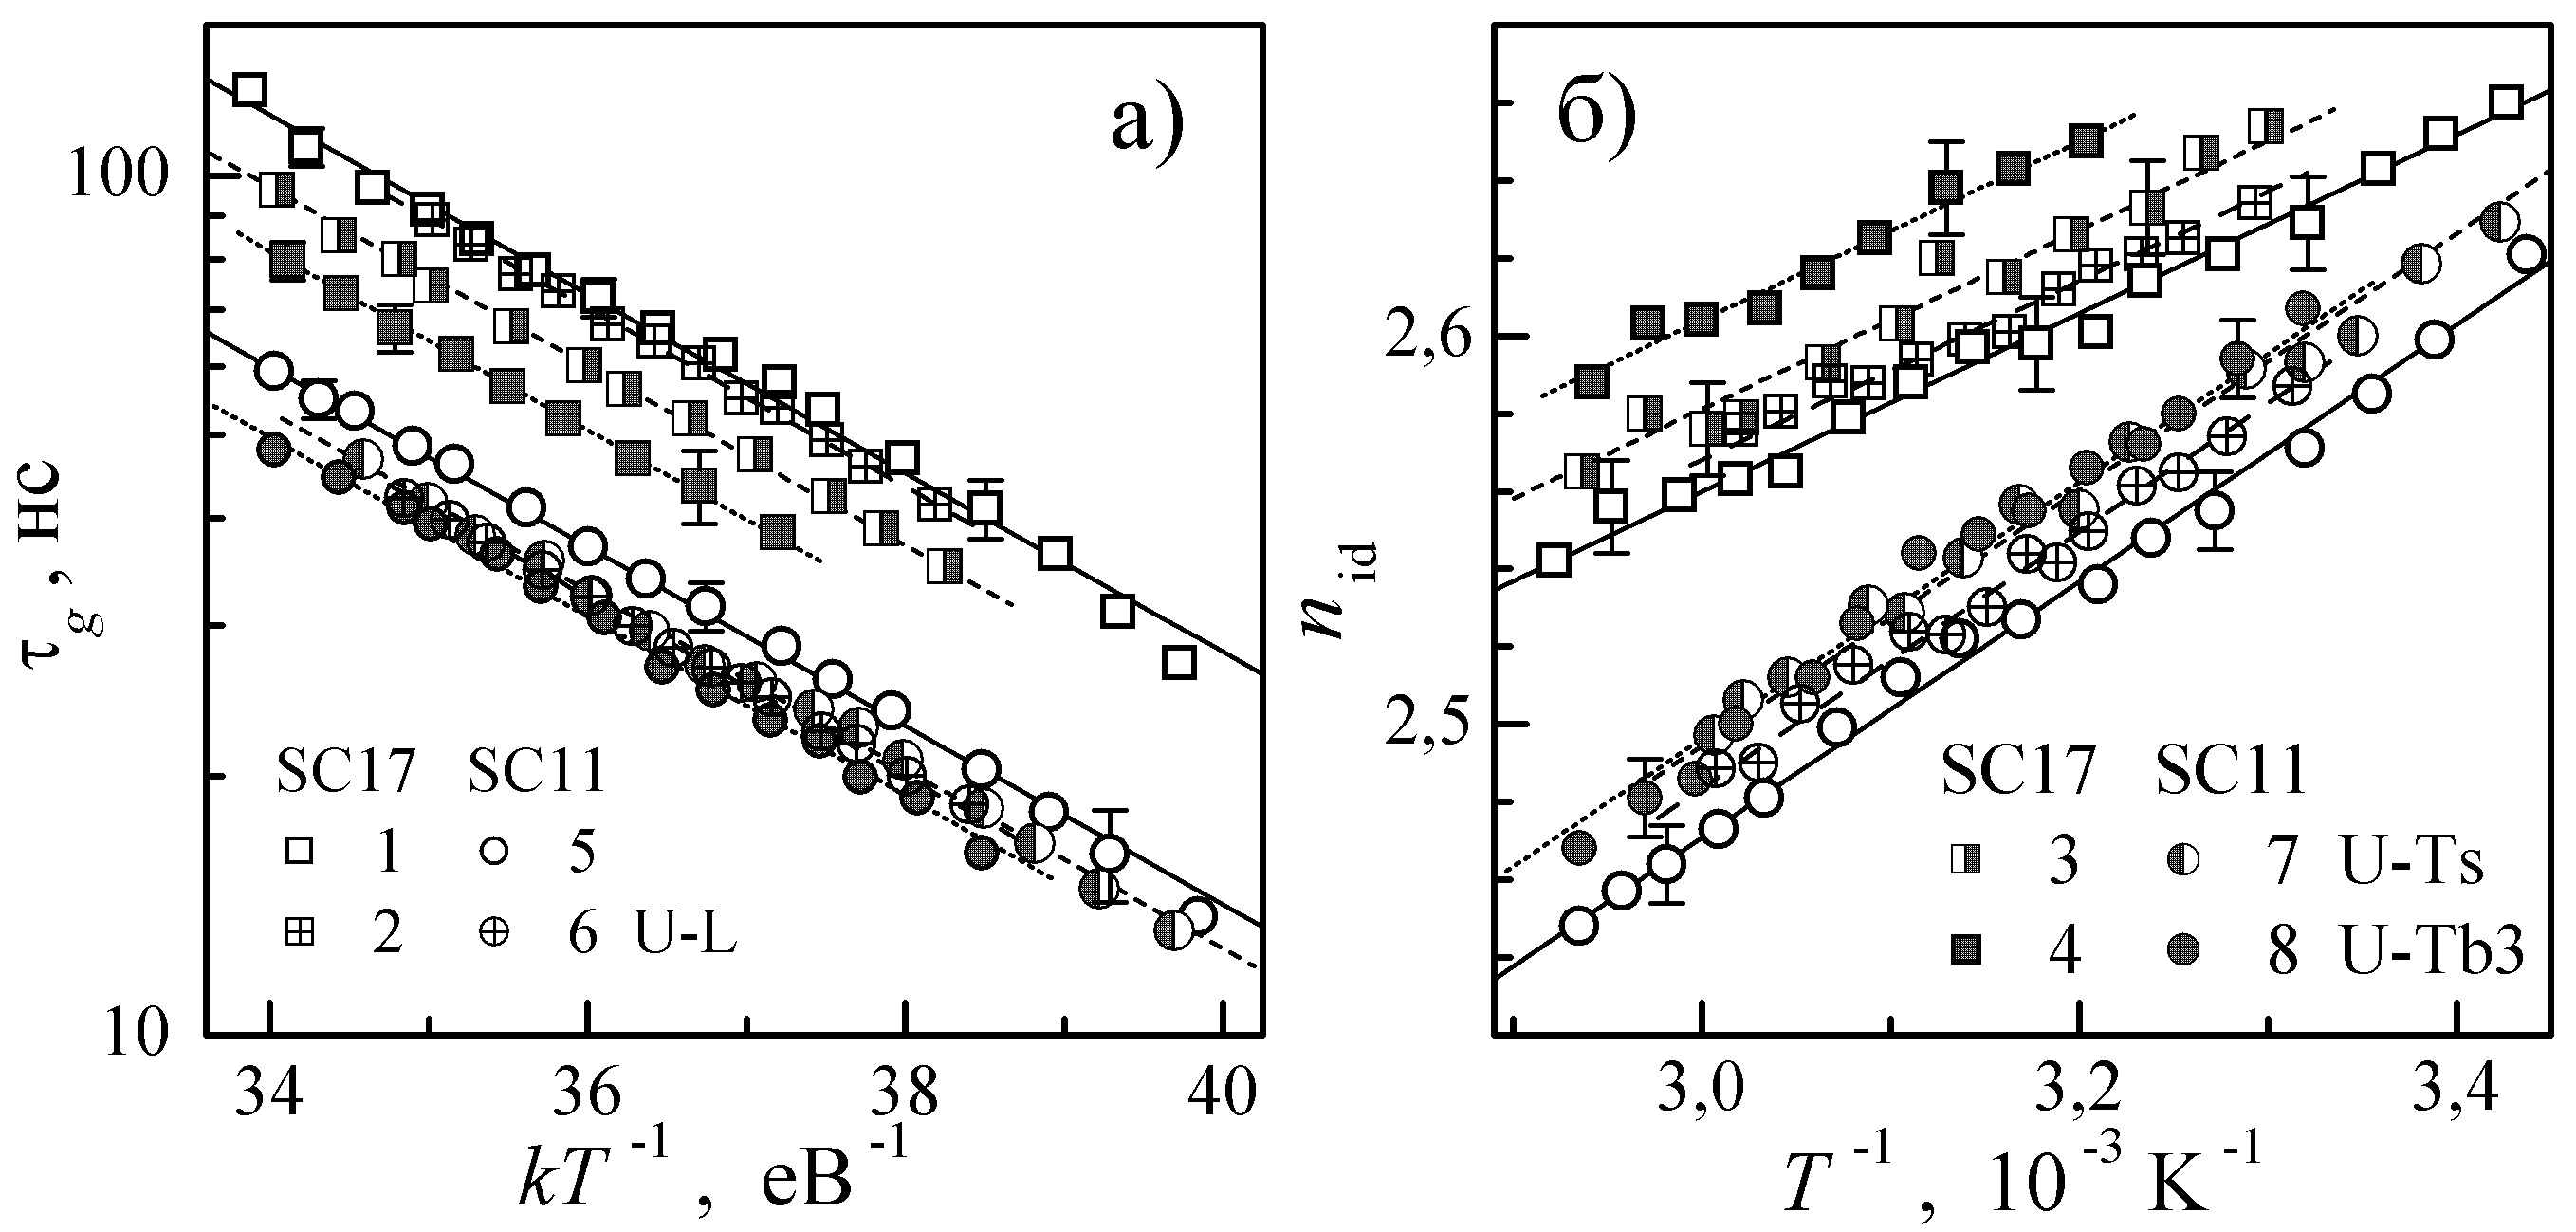
\includegraphics[width=1\textwidth]{figDUS}%
\caption{\label{figDUS}
Температурні залежності часу життя носіїв в ОПЗ (а) та фактору неідеальності (б)
для зразків SC17 (криві 1--4, квадрати) та SC11 (5--8, кола).
\FigCaptionSSC
Точки --- експеримент,
лінії -- результат апроксимації з використанням виразу~(\ref{eq_TAUgT}) і $E_{\tau g}=0.24$~eV (a) та
формули~(\ref{eq_nT}) і $T_\mathrm{id}=330$ або 230~K (б).
}%
\end{figure}

Як показано на Рис.~\ref{figDUS},б, фактор неідеальності зменшується зі зростанням температури, а залежність
$n_{\mathrm{id}}$ від $1/T$  близька до лінійної.
Таким чином, залежність $n_{\mathrm{id}}(T)$ може бути описана наступним чином
\begin{equation}
\label{eq_nT}
    n_{\mathrm{id}}(T)=n_{\mathrm{id},\infty}+T_{\mathrm{id}}/T\:.
\end{equation}
Величини $T_{\mathrm{id}}$ та $E_{\tau g}$, обчислені для зразків в умовах УЗН та без нього, наведено в Таблиці~\ref{tabSSCParam}.


Як видно з наведених на Рис.~\ref{figDUS} та в Таблиці~\ref{tabSSCParam} даних
\begin{enumerate}[label=\asbuk*),leftmargin=0em,itemindent=1.5em]
%\begin{enumerate}[label=\asbuk*),labelindent=0em,itemindent=1.5em]
\item УЗН призводить збільшення $n\mathrm{id}$ та зменшення $\tau_{g}$;
   величини АІ змін показано в Таблиці~\ref{tabAIEfect};
\item $\tau_{g}$ та $n\mathrm{id}$ змінюються більш ефективно при використанні поперечних АХ;
\item $\varepsilon_{\tau g}$ та $\Delta n_\mathrm{id}$ збільшуються при використанні УЗ з більшими значеннями $W_{\mathtt{US}}$;
\item УЗН не впливає на $E_{\tau g}$ та $T_\mathrm{id}$;
 $E_{\tau g}=0.24\pm0.01$~еВ для всіх досліджених зразків,
 тоді як характерна температура фактору неідеальності залежить від місця розташування зразка на пластині: $T_\mathrm{id}=330\pm30$~K для SC11 та $T_\mathrm{id}=230\pm20$~K для SC17.
\end{enumerate}

Для проведення аналізу отриманих результатів важливо визначити механізм рекомбінації в ОПЗ досліджених зразків.
При цьому необхідно звернути увагу, насамперед, на велике значення  $n_{\mathrm{id}}$ та малі значення $\tau_g$.

Відповідно до класичної теорії Шоклі--Ріда--Хола (ШРХ),
фактор неідеальності має бути не більшим ніж 2, а температурна залежність $\tau_g$ має описуватися виразом \cite{TAUg:Schroder,TAUg:Aharoni}:
\begin{equation}
  \tau_g\simeq2\,\tau_n\sqrt{\frac{\sigma_n}{\sigma_p}}\cosh\left(\frac{E_t-E_i}{kT}\right)
\end{equation}
де
$\sigma_n$ та $\sigma_p$ --- поперечні перерізи захоплення (ППЗ) електронів та дірок, відповідно,
рекомбінаційним центром;
$E_t$ --- положення енергетичного рівня, зв'язаного з цим центром,
$E_i$  --- положення рівня Фермі у власному напівпровіднику.
В нашому випадку значення $n_{\mathrm{id}}$ більші ніж 2,
а $\tau_g$ експоненційно зростає з підвищенням температури.
Тобто теорія ШРХ не є застосовною.

В літературі для пояснення великих значень фактору неідеальності, які нерідко зустрічаються на практиці,
запропоновано декілька моделей.
Наприклад, згідно з \cite{Heide}, неоднорідність фронтального металізованого контакту може викликати появу значних величин $n_\mathrm{id}$.
Проте це модель передбачає, що фактор неідеальності має залежати від інтенсивності освітлення, тоді як в нашому випадку змін $n_\mathrm{id}$ для різних
значень $W_{ph}$ не спостерігалося.
Beier та Voss \cite{Beier} пояснюють великі можливі значення $n_\mathrm{id}$ ефектами насичення (пов'язаними з наявністю декількох
рекомбінаційних центрів) в рамках моделі ШРХ.
Проте це теорія не здатна пояснити величини $J_{0SCR}$, які в нашому випадку значно перевищують очікувані, згідно з теорією ШРХ, значення для кремнію.
Крім того, значні величини фактору неідеальності також пов'язуються з тунелюванням за участю глибоких рівнів (ГР)\cite{Shah,Kaminski_n}.
Проте при такому підході $n_\mathrm{id}$ не має залежати від температури.

В той же час, всі експериментально спостережені особливості рекомбінації в ОПЗ можуть бути пояснені в рамках
моделі рекомбінації у системі спарених рівнів дефектів (CDLR, coupled defect level recombination).
Цей механізм передбачає швидкі переходи носіїв заряду безпосередньо між рівнями, які належать різним дефектам,
розташованим поблизу один одного.
Це явище спочатку було виявлене експериментально \cite{DAPR:Chen1991,DAPR:Chen1994},
а потім використане для пояснення процесів, які відбуваються у напівпровідникових діодах \cite{CDLR:JAP1995,CDLR:JAP,CDLR:SSP,Breitenstein2013,CDLR:SupMicr}.
На початкових етапах розвитку моделі вважалося \cite{CDLR:JAP1995}, що щонайменше один з рівнів має бути
мілким.
Надалі було запропоновано, що такі процеси можуть проходити і за участю дефектів, рівні яких не розташовані близько до границь дозволених зон;
проте темп рекомбінації буде максимальним, якщо дефект акцепторного типу утворює пару з дефектом донорного типу \cite{CDLR:JAP}.
Надалі, для скорочення замість термінів <<дефект акцепторного типу>> та <<дефект донорного типу>>
будемо використовувати <<акцептор>> та <<донор>>, не маючи на увазі, що завдяки цим дефектом суттєво змінюється провідність кристалу.
Зазначимо, що в цьому випадку мова не йде про утворення стійкої конфігурації на кшталт комплексного точкового дефекту (ТД),
між компонентами якого виникає високоінтенсивний зв'язок.
У запропонованій парі (acceptor--like defect is coupled with donor-like defect) складові взаємодіють
між собою лише внаслідок того, що електрон з рівня однієї (наприклад, донора) може переходити на рівень іншої (наприклад, акцептора).

Принагідно зауважимо, що це не єдина модель, згідно з якою у рекомбінації приймає участь два
дефектні рівні.
Так нещодавно \cite{TwoLevelRecomb} був запропонованих механізм, який передбачає, що рівень, поблизу дна зони провідності
на який ефективно захоплюються електрони і рівень недалеко від вершини валентної зони, який ефективно захоплює дірки,
належать одному дефекту, що може перебувати у двох конфігураціях залежно від зарядового стану.
Процеси захоплення носіїв із зон супроводжуються швидкою структурною трансформацією дефекту між стабільною та метастабільною конфігураціями.

Повертаючись до моделі CDLR,
зауважимо, що згідно з нею високі значення фактору неідеальності пов'язані з насиченням
міжрівневого рекомбінаційного каналу.
Крім того, очікується \cite{CDLR:JAP,Breitenstein2013}, що
на залежності диференційного фактору неідеальності
$n_\mathtt{id}^\mathtt{dif}=\frac{1}{kT}\frac{dV}{d(\ln I)}$ від прикладеної напруги має
спостерігатися максимум, величина та розташування якого залежить від енергетичного положення та
ППЗ рівнів, а також від характеристик міжрівневої рекомбінації.
Саме така залежність спостерігається і для досліджених структур --- див. Рис.~\ref{figdidV}.

\begin{figure}
\center
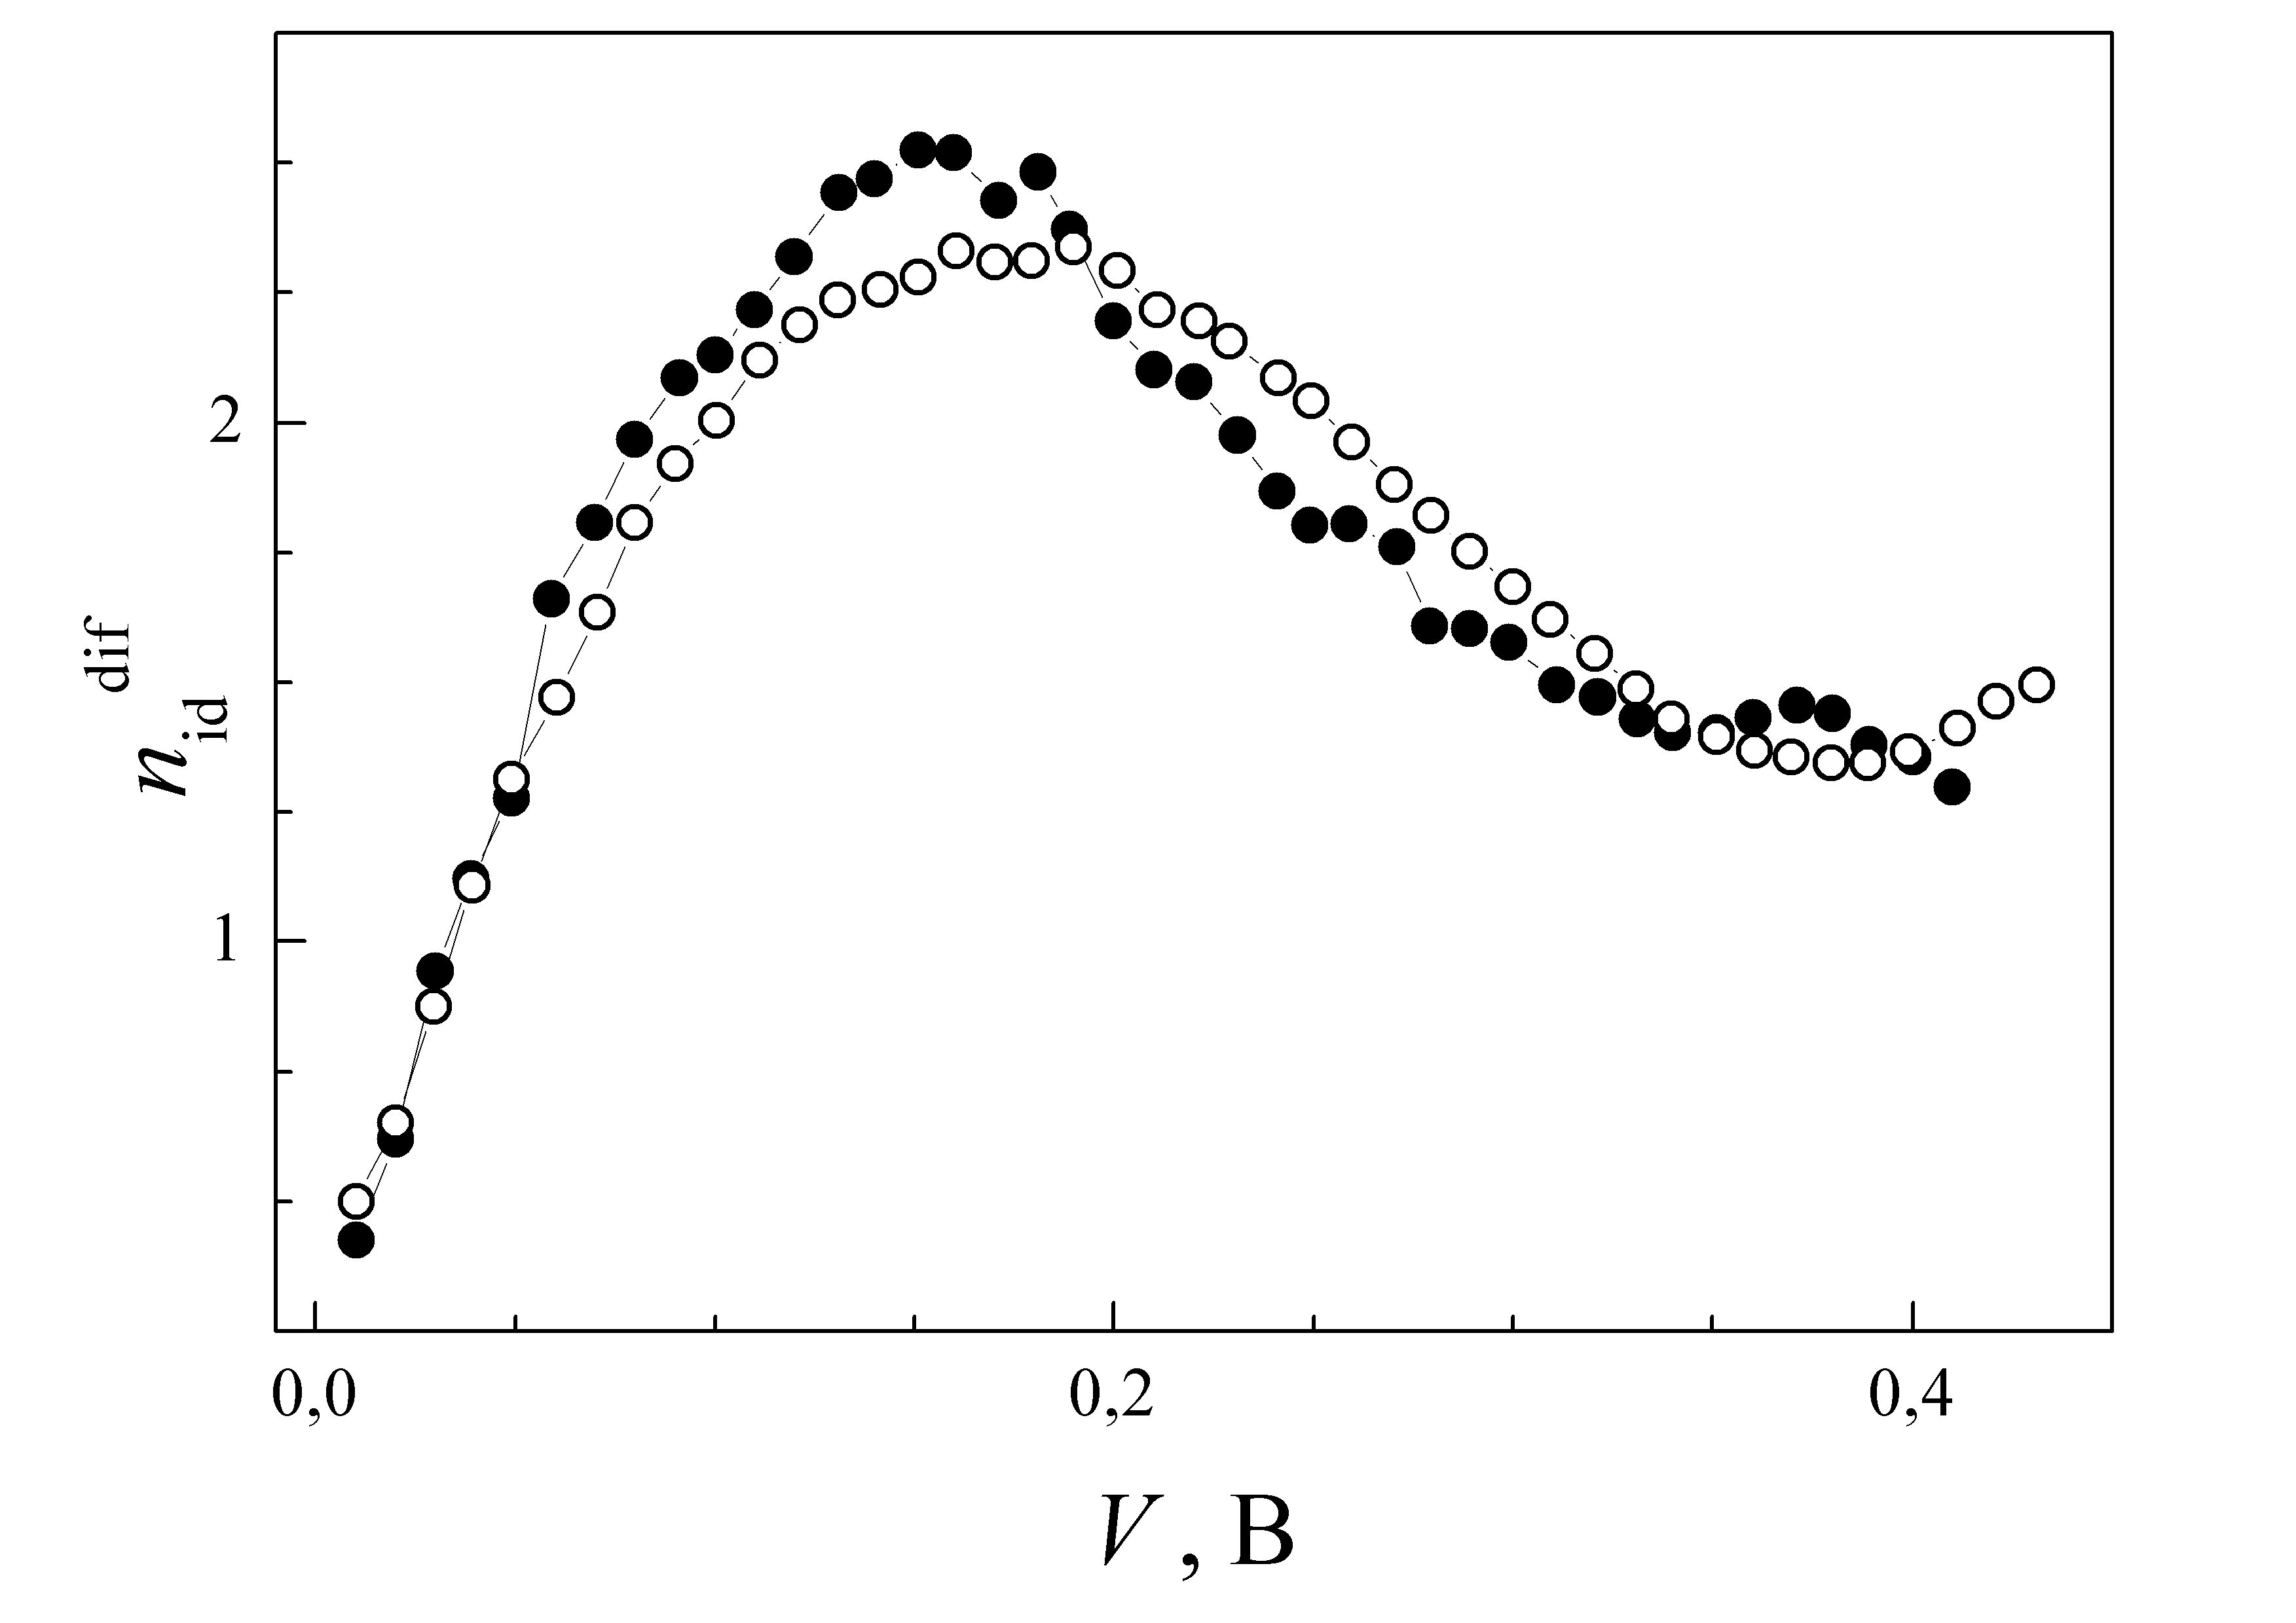
\includegraphics[width=0.6\textwidth]{figdidV}%
\caption{\label{figdidV}
Залежність диференційного фактору неідеальності від напруги.
Незаповнені точки --- без УЗН, заповнені --- при УЗН U--Tb3.
Зразок SC17, $T=335$~К.
}%
\end{figure}
%In this deep DAP model the high ideality factor is due to
%saturation of the inter−level recombination channel, leading
%to a hump in the n(V) characteristics. It was found that the
%magnitude and the position of this hump strongly depends
%on the energy positions and on the capture and inter−level
%recombination parameters of the two levels involved.

%Повертаючись до CDLR, наголосимо, що
У спрощеному випадку, коли відсутні переходи між рівнем донора $E_t^{\mathtt{D}}$ та валентною зоною
і між рівнем акцептора $E_t^{\mathtt{A}}$ та зоною провідності,
темп рекомбінації у системі спарених рівнів $R$ може бути описаний наступним виразом \cite{CDLR:JAP1995}:
\begin{eqnarray}
R&=&\frac{R_{12}-\sqrt{R_{12}^{\,2}-4\tau_{n}^{\mathtt{D}}\tau_{p}^{\mathtt{A}}(np-n_i^2)(1-\epsilon)}}{2\tau_{n}^{\mathtt{D}}\tau_{p}^{\mathtt{A}}(1-\epsilon)}\;,\label{eqR}\\
R_{12}&=&\frac{(n+n_{\mathtt{D}})(p+p_{\mathtt{A}})}{R_{\mathtt{DA}}}+
\tau_{n}^{\mathtt{D}}(p+p_{\mathtt{D}})+\tau_{p}^{\mathtt{A}}(n+n_{\mathtt{A}}),\label{eqR12}\\
\tau_{n}^{\mathtt{D}}&=&(N_{\mathtt{D}}\,\sigma_{n}^{\mathtt{D}}\,\upsilon_{\mathrm{th},n})^{-1},\,\,\,\,
\tau_{p}^{\mathtt{A}}=(N_{\mathtt{A}}\,\sigma_{p}^{\mathtt{A}}\,\upsilon_{\mathrm{th},p})^{-1},\label{eqTAU}
\end{eqnarray}
де
$R_{\mathtt{DA}}$ --- так званий параметр зв'язку,
$N_{\mathtt{D}}$ та $N_{\mathtt{A}}$ --- густини донорів та акцепторів, відповідно;
$\sigma_{n}^{\mathtt{D}}$ та $\sigma_{p}^{\mathtt{A}}$ --- ППЗ електронів донором та дірок акцептором, відповідно;
$\upsilon_{\mathrm{th},n}$ та $\upsilon_{\mathrm{th},p}$ --- теплові швидкості електронів та дірок, відповідно;
$n_{\mathtt{D,A}}$, $p_{\,\mathtt{D,A}}$ та $\epsilon$ залежать від $E_t^{\mathtt{D}}$, $E_t^{\mathtt{A}}$ та факторів виродження рівнів.

Відповідно до \cite{CDLR:JAP},
ППЗ для дефекту в парі відрізняється від значення, характерного для ізольованого дефекту, і залежить від відстані $r$ між донором та акцептором
\begin{equation}
\label{eqSigma}
\sigma_{n,p}^{\mathtt{D,A}}(r)=C_{n,p}^{\mathtt{D,A}}\,r^2\,,
\end{equation}
де $C_{n}^{\mathtt{D}}$ та $C_{p}^{\mathtt{A}}$ --- певні константи.
Величина $R_{\mathtt{DA}}$ також залежить від $r$ та пропорційна інтегралу перекриття хвильових функцій дефектів.
Зокрема, якщо і донор, і акцептор характеризується водне--подібними хвильовими функціями і однаковим радіусом Бора $a_B$, то \cite{CDLR:JAP}
\begin{equation}
\label{eqRda}
R_{\mathtt{DA}} (r) \sim N_{\mathtt{D}}N_{\mathtt{A}}\left[1+\frac{r}{a_B}+\frac{1}{3}\left(\frac{r}{a_B}\right)^2\right]
   e^{-r/a_0}\,.
\end{equation}

На жаль, вираз, який би дозволяв аналітично описати взаємозв'язок між параметрами ВАХ (наприклад, $n_{\mathrm{id}}$ та $\tau_g$)
і характеристиками дефектів, які беруть участь У CDLR, відсутній.
Однак, показано \cite{CDLR:JAP1995,CDLR:SSP} що $n_{\mathrm{id}}$ збільшується зі зменшенням $R_{\mathtt{DA}}$.
Так як $\tau_g\sim R^{-1}$,
то видається цілком очікуваним, що $n_{\mathtt{D,A}}$, $p_{\,\mathtt{D,A}}$ та $\epsilon$ забезпечують термоактиваційний характер часу життя носіїв в ОПЗ.
На нашу думку, величина $E_{\tau g}$ насамперед визначається енергетичними рівнями зв'язаних дефектів, тобто
залежить від їх типу та конфігурації.
В той же час, значення $T_\mathrm{id}$ залежить також і від $N_\mathtt{D}$ та $N_\mathtt{A}$.
Таким чином, отримані результати свідчать, що
\begin{enumerate}[label=\asbuk*),leftmargin=0em,itemindent=1.5em]
\item у рекомбінаційних процесах як в SC11, так і в SC17 приймають участь однакові дефекти, так як значення $E_{\tau g}$ збігається;
\item концентрація рекомбінаційно--активних дефектів у зразках різна, про що свідчать неоднакові значення $T_\mathrm{id}$, $\tau_{g,in}$ та $n_{\mathrm{id},in}$;
\item УЗН не призводить до змін енергетичних рівнів та концентрацій дефектів, так як  $E_{\tau g}$ та $T_\mathrm{id}$ в умовах поширення АХ не міняються.
\end{enumerate}

При записі виразу для $J_{base}$ (див. формулу (\ref{eqSSCIV})) вважалося, що дифузійний струм виникає внаслідок інжекції
електронів з емітера в базу.
Загалом, при проходженні струму відбуваються також процеси інжекції дірок з бази в емітер, проте для несиметричного $p-n$ переходу
($n_n\gg p_p$) цією складовою можна знехтувати \cite{Breitenstein2013}.
Крім того, вираз $J_{0base}=(qn_i^2/n_n)\sqrt{\mu_nkT/\tau_n}$ справедливий лише за умови, що товщина бази у декілька разів перевищує
довжину дифузії неосновних носіїв \cite{Sze2012}.
Як показують дані Таблиці~\ref{tabSSCParam}, ця умова в нашому випадку також виконується.

Величина $J_{0base}=(qn_i^2/n_n)\sqrt{\mu_nkT/\tau_n}$ відображає процеси, що відбуваються в КНО сонячного елементу.
Під час аналізу  вважалося, що $n_n$ та $\mu_n$ не залежать від УЗН.
Підставами для цього бути
а)~експериментально виявлена незалежність послідовного опору від УЗН;
б)~загальновідомий факт, що для дослідженого температурного діапазону рухливість визначається насамперед розсіянням на атомах ґратки.
У зв'язку з цим основна увага була приділена $\tau_n$, температурна поведінка якого показана на Рис.~\ref{figDUSTau}.
Як і очікувалось відповідно до літературних даних, час життя неосновних носіїв збільшується з підвищенням температури.
Визначені шляхом апроксимації експериментальних залежностей значення $\tau_n$ та розраховані на їх основі величини $L_n$,
а також їх зміни в умовах УЗН наведено в Таблицях~\ref{tabSSCParam} та \ref{tabAIEfect}.
Наведені результати показують, що УЗН призводить до зменшення $\tau_n$, причому ефект достатньо значний:
при поширення АХ значення часу життя може зменшуватись до 20~\% вихідної значення.

Отримані таким чином величини $L_{n,in}$ цілком співрозмірні зі значеннями $L_{n,in}^{ph}$, отримані на основі аналізу залежностей $J_{sc}(T)$.
Невеликі кількісні відмінності між $\varepsilon_{L n}^{ph}$ та $\varepsilon_{L n}$,
на нашу думку, пов'язані з певною АІ зміною температурної залежності довжини дифузії (див. Рис.\ref{figDUSTau}),
яка не враховувалася під час апроксимації температурної залежності струму короткого замикання.


\begin{figure}
\center
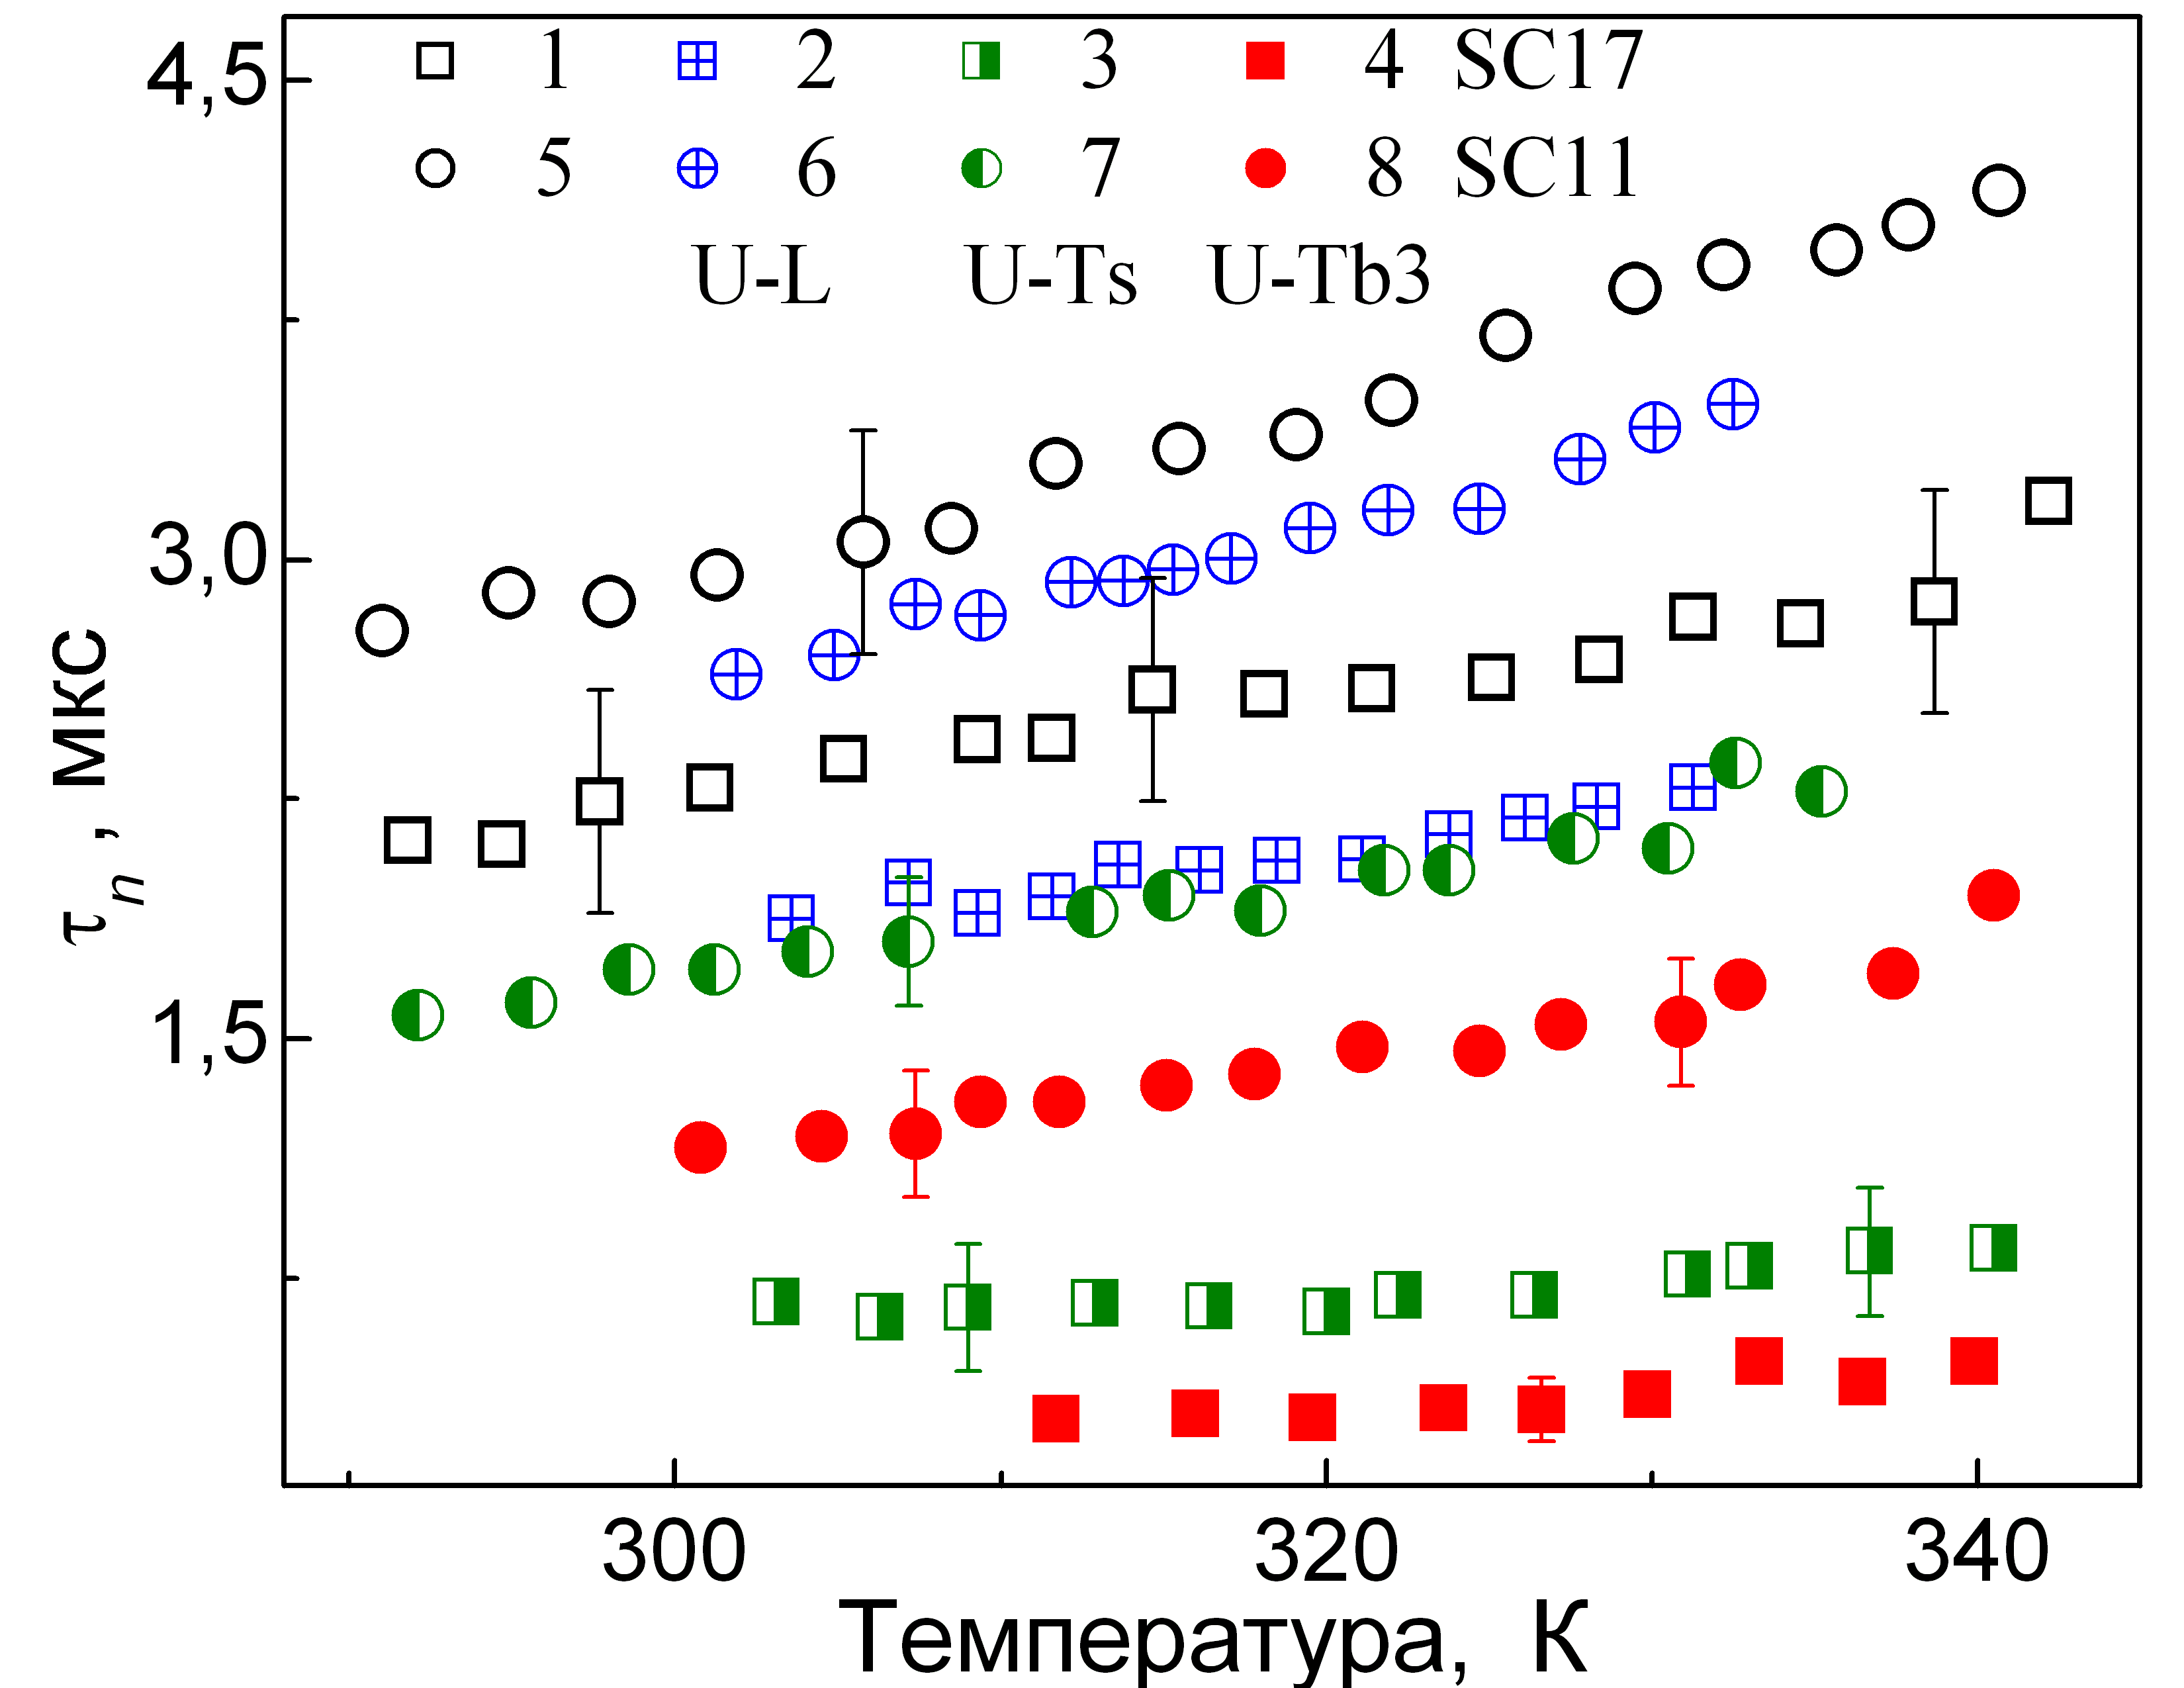
\includegraphics[width=0.7\textwidth]{figDUSTau}%
\caption{\label{figDUSTau}
Температурні залежності часу життя неосновних носіїв в КНО
для зразків SC17 (криві 1--4, квадрати) та SC11 (5--8, кола).
\FigCaptionSSC
}%
\end{figure}

Час життя неосновних носіїв в загальному випадку описується наступним чином \cite{MurphyJAP2011}:
\begin{equation}
\label{eqTAUsum}
\tau_n^{-1}=\tau_\mathtt{bb}^{-1}+\tau_\mathtt{CE\,Auger}^{-1}+\tau_\mathtt{SRH}^{-1}\,,
\end{equation}
де
$\tau_\mathtt{bb}$ --- час життя, пов'язаний з випромінювальною міжзонною рекомбінацією
\begin{equation}
\label{eqTAUbb}
\tau_\mathtt{bb}^{-1}=B(p_p+n_p+\Delta n)\,,
\end{equation}
$B$ --- коефіцієнт міжзонної рекомбінації, $B=1\cdot10^{-14}$~см$^3$c$^{-1}$ \cite{Si:TAUbb,MurphyJAP2011},
$\Delta n$ --- концентрація нерівноважних електронів,
$\tau_\mathtt{CE\,Auger}$ визначається Оже--рекомбінацією, підсиленою внаслідок кулонівської взаємодії  \cite{Si:TAUAuger}
\begin{equation}
\label{eqTAAuger}
\tau_\mathtt{CE\,Auger}=\frac{\Delta n}{np\left(1,8\cdot10^{-24}n_p^{0,65}+6\cdot10^{-25}p_p^{0,65}+3\cdot10{-27}\Delta n^{0.8}\right)}\,,
\end{equation}
$n$ та $p$ --- концентрації електронів та дірок, відповідно;
$\tau_\mathtt{SRH}$ --- час рекомбінації ШРХ.
В наших дослідах $\Delta n$ не перевищувала $8\cdot10^{13}$~см$^{-3}$.
Як наслідок, розрахунки показали, що $\tau_\mathtt{bb}^{-1}\leq14$~с$^{-1}$, $\tau_\mathtt{CE\,Auger}^{-1}\leq6$~с$^{-1}$.
А отже, міжзонною рекомбінацією та рекомбінацією Оже можна знехтувати, $\tau_n=\tau_\mathtt{SRH}$.

За умови низького рівня інжекції якщо в кристалі присутні декілька рекомбінаційних центрів $\tau_\mathtt{SRH}$ описується виразом

\begin{equation}
\label{eqTAUSHRsum}
\tau_n^{-1}=\sum_i^{M_d}\tau_{n,i}^{-1}=\sum_i^{M_d}N_{d,i}\,\sigma_{n,i}\,\upsilon_{\mathrm{th},n}\,,
\end{equation}
де
$M_d$ --- загальна кількість типів центрів,
$\tau_{n,i}$ описує час життя при рекомбінації лише за участю дефектів $i$--го типу,
які характеризуються концентрацією $N_{d,i}$ та ППЗ електронів $\sigma_{n,i}$.

На Рис.~\ref{figKus} наведено залежність оберненого часу життя в ОПЗ від параметрів УЗН,
причому в одному випадку таким параметром вибрана $W_{U\!S}$, а в другому ---$u_\mathtt{US}^2$.
Видно, що $\tau_n^{-1}$ лінійно зростає з підвищенням інтенсивності введеного УЗ,
тобто АІ зміни часу життя можна записати у вигляді

\begin{figure}
\center
%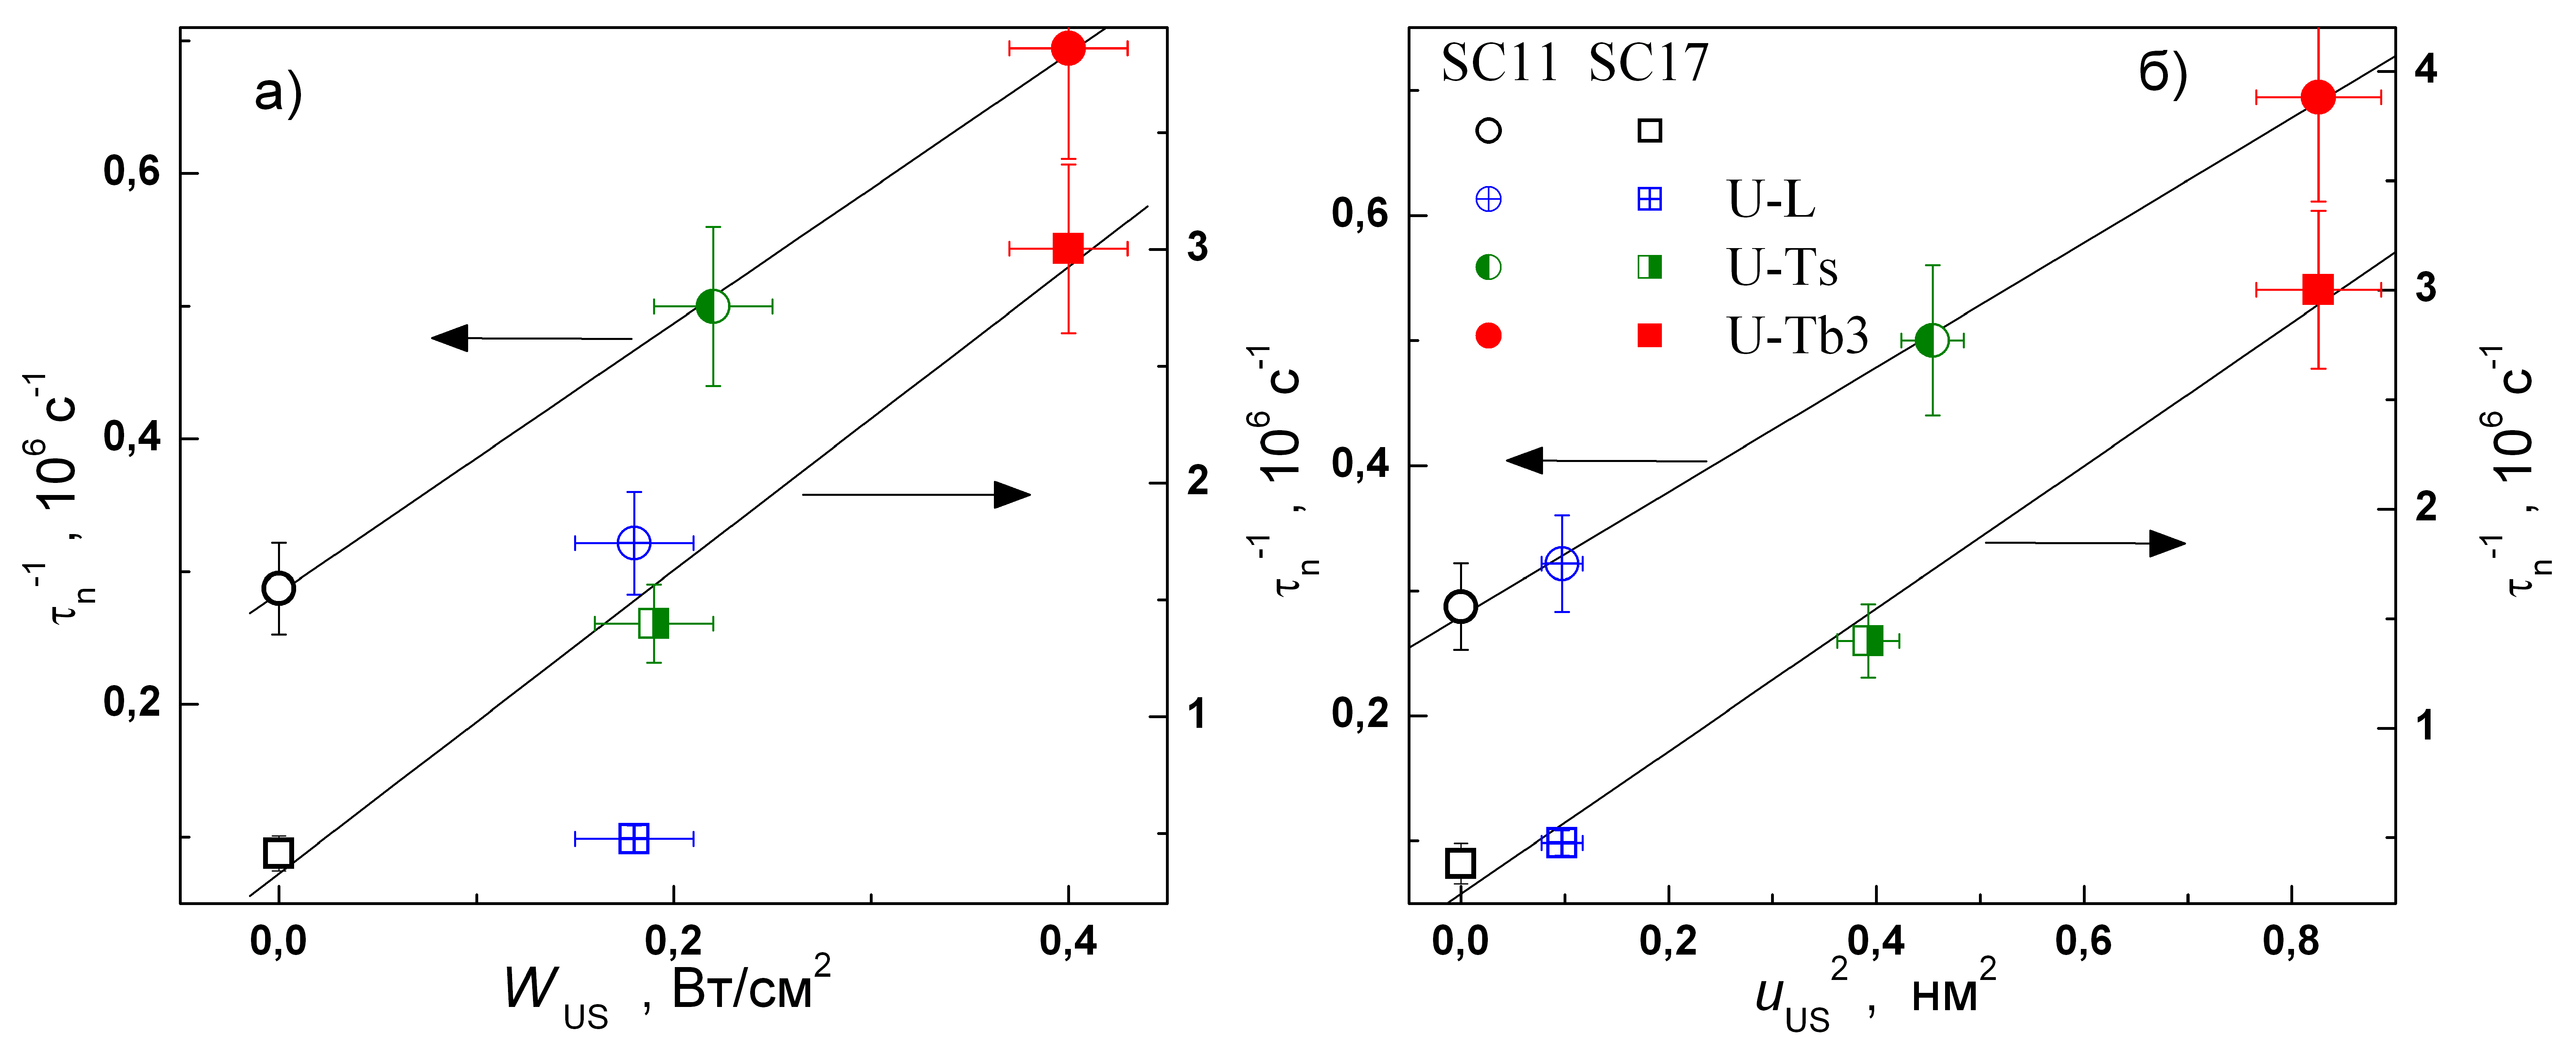
\includegraphics[width=1\textwidth]{figKus}%
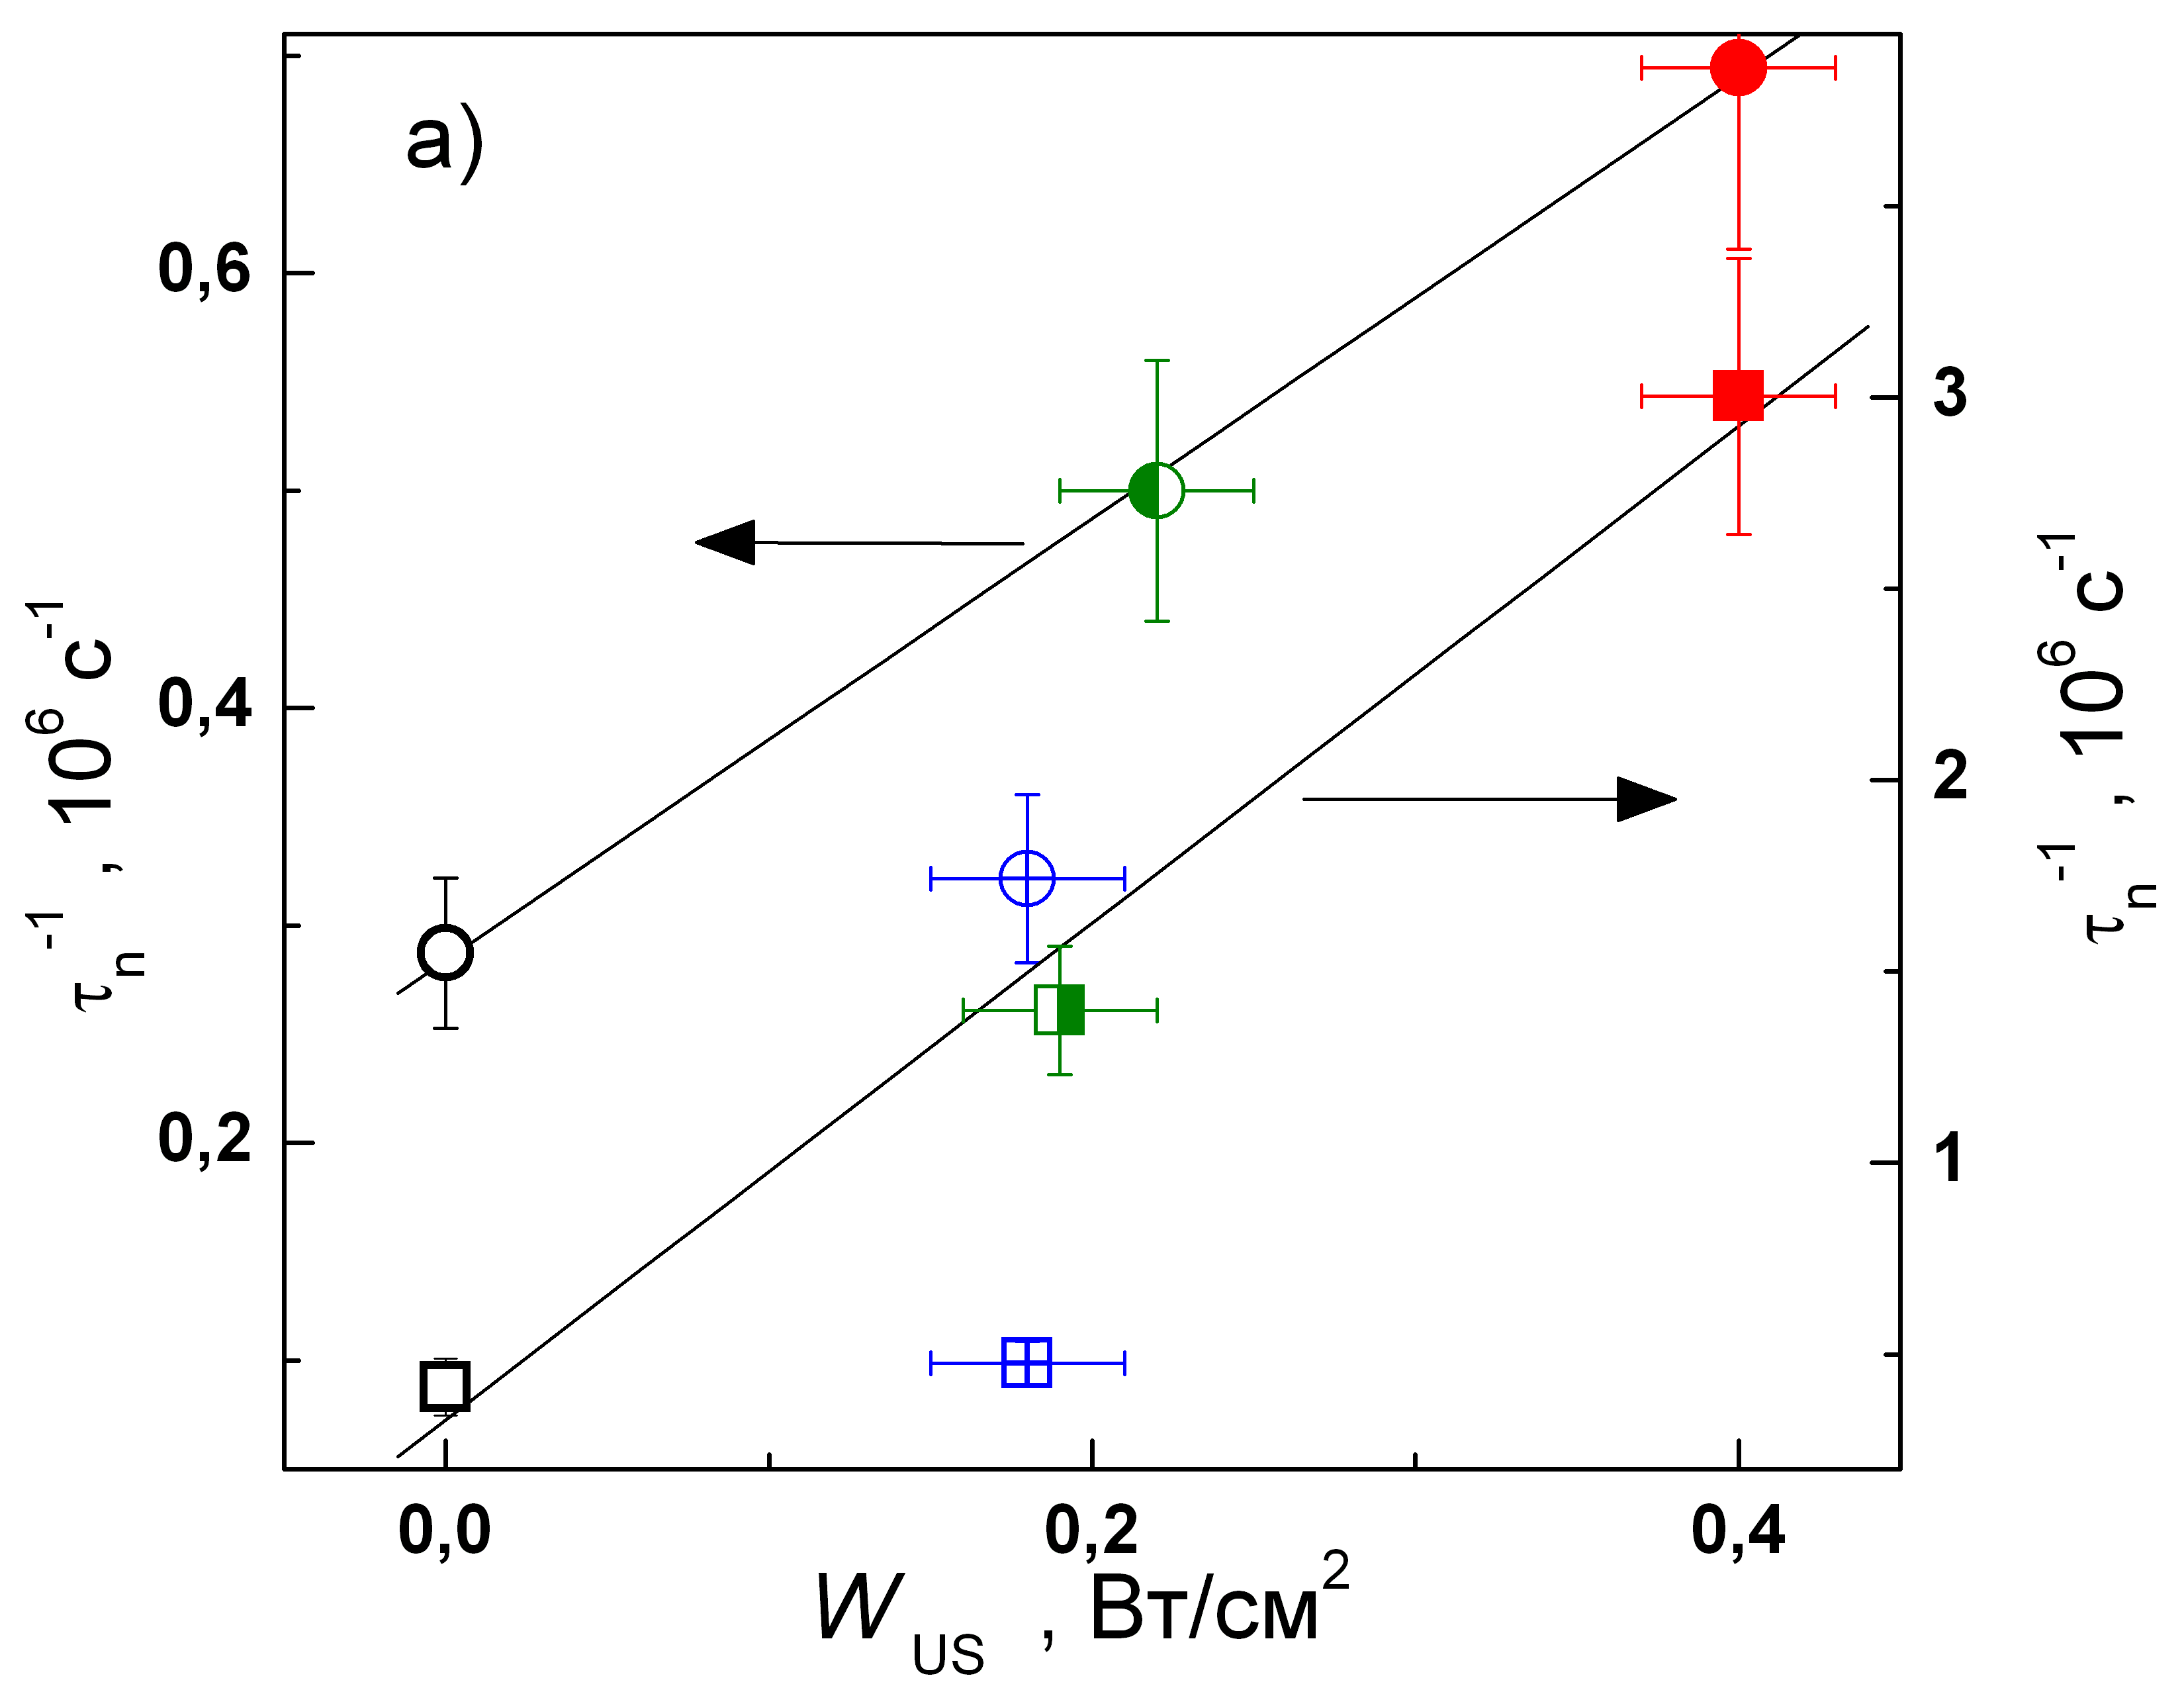
\includegraphics[width=0.49\textwidth]{figKus_a} \hfill
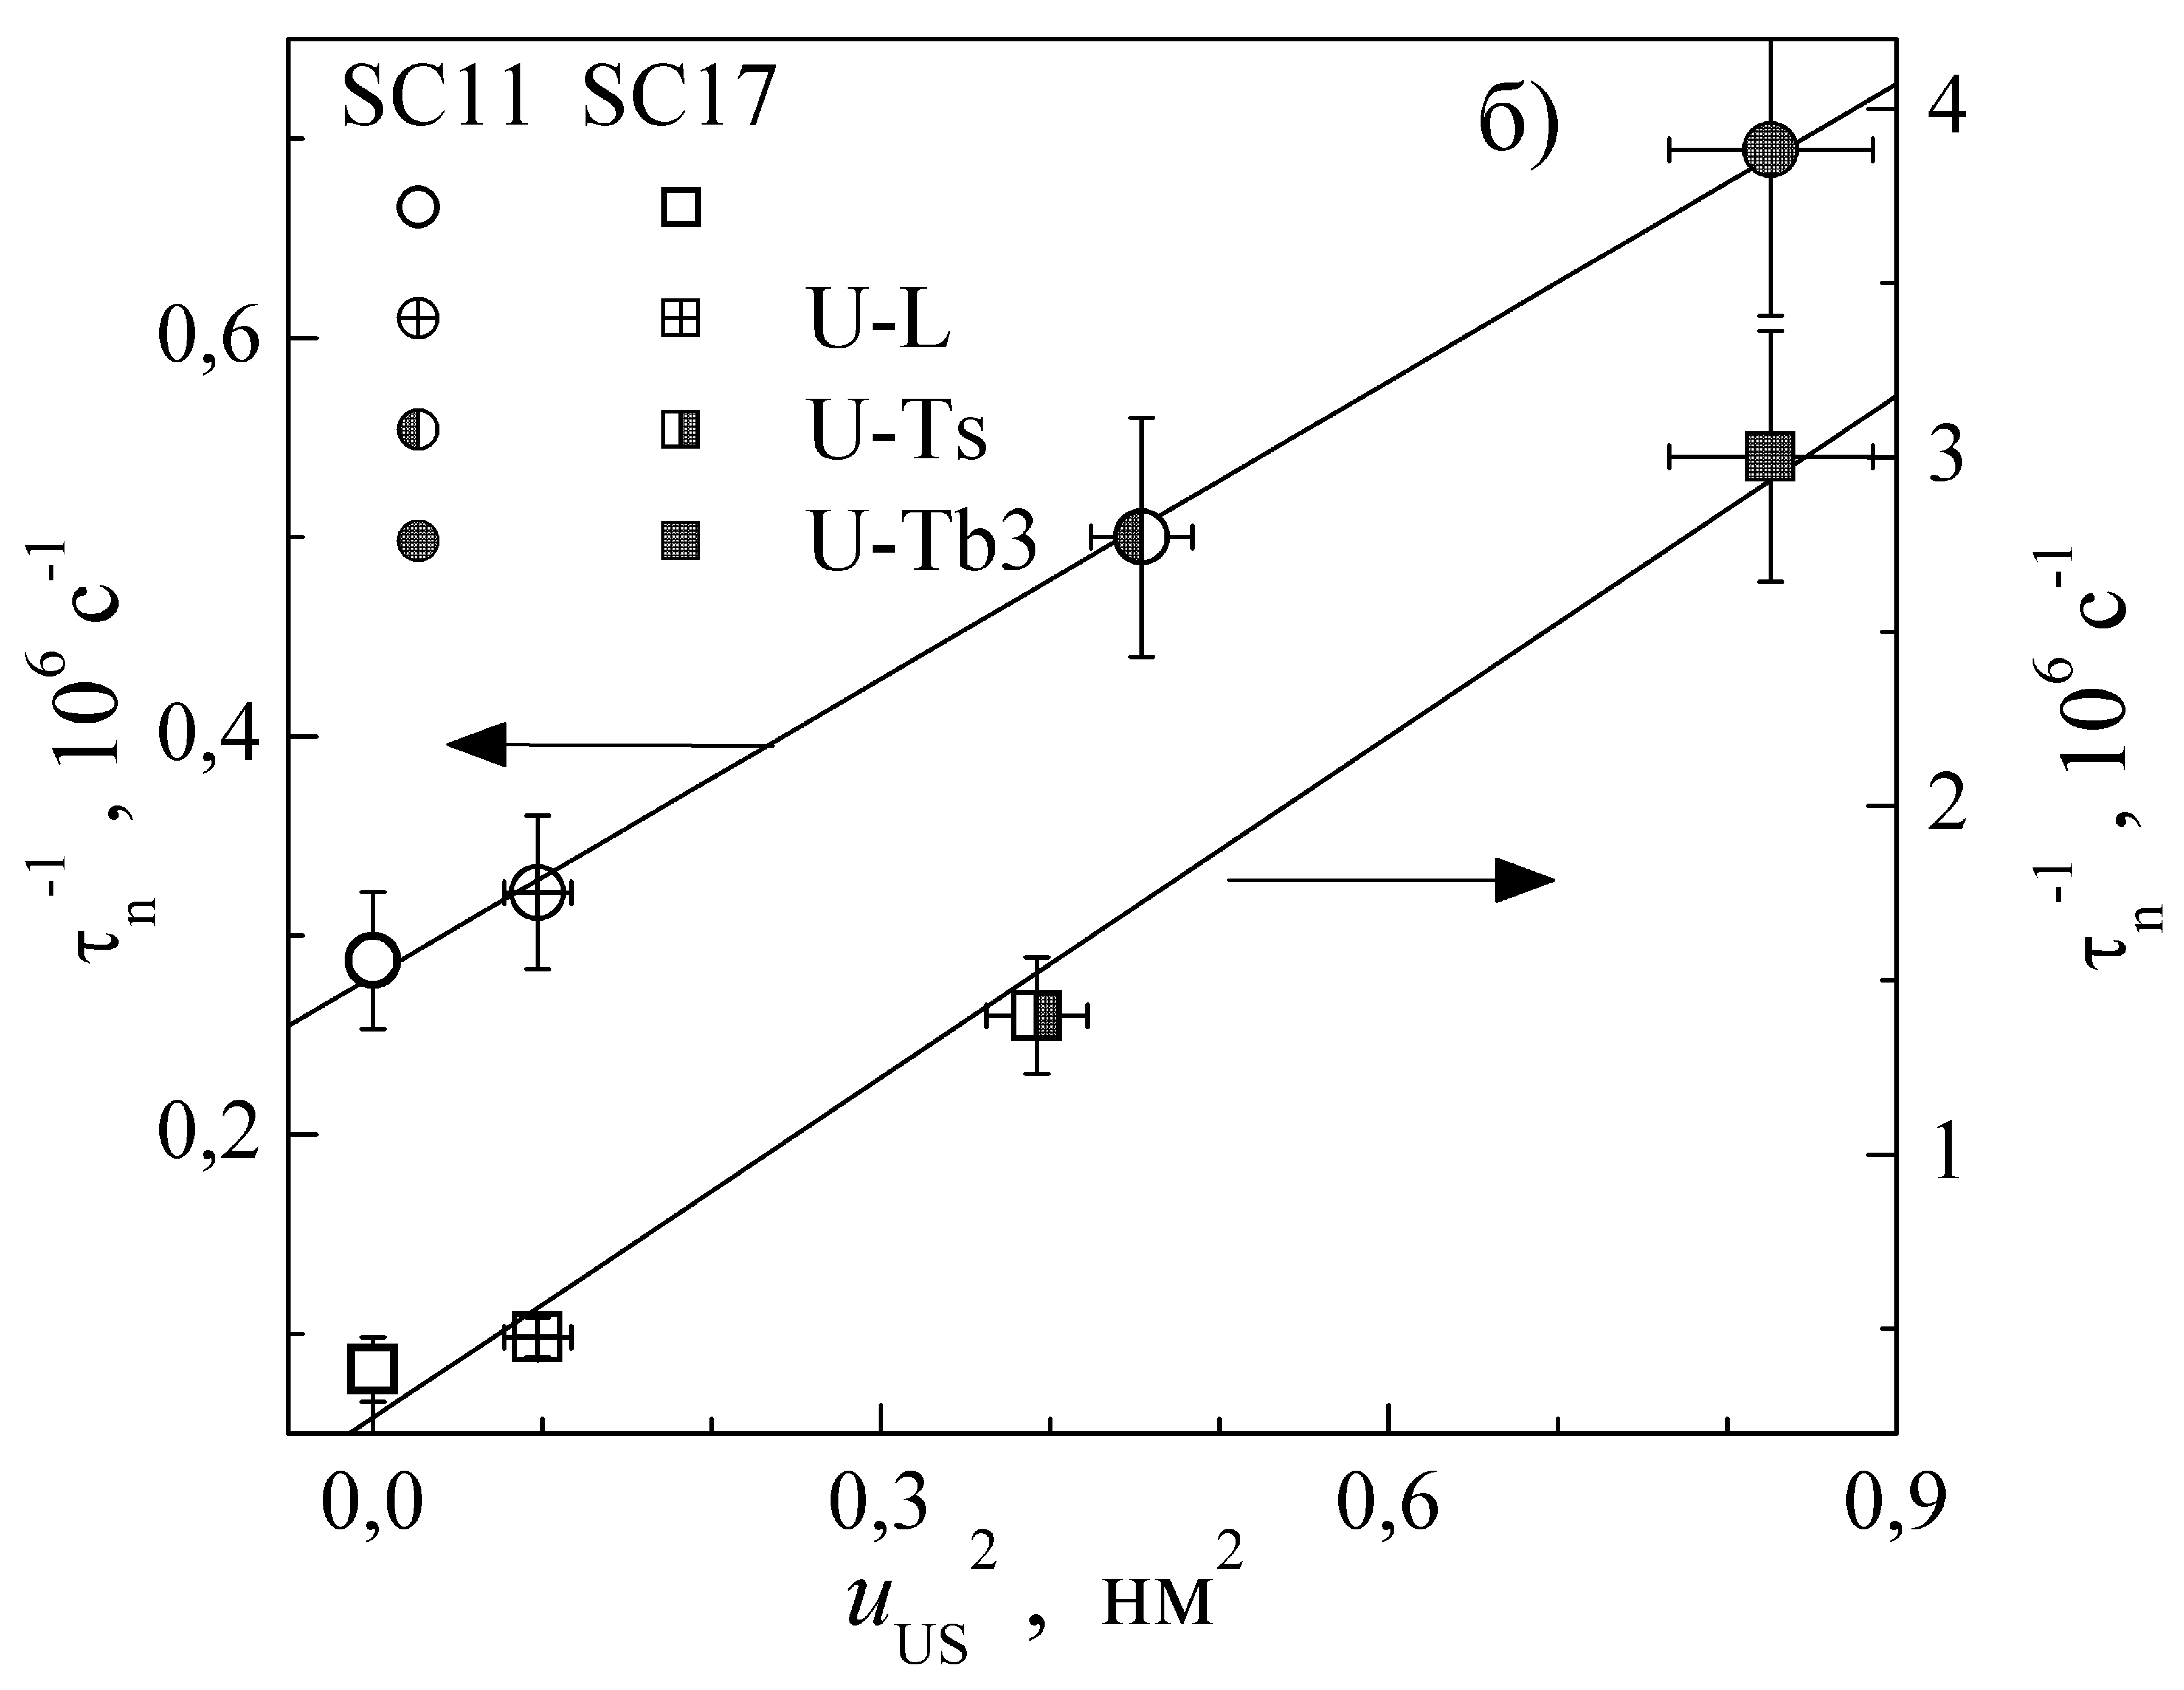
\includegraphics[width=0.49\textwidth]{figKus_b}
\caption{\label{figKus}
Залежність оберненого часу життя в ОПЗ від інтенсивності введеного звуку (а)
та від квадрату амплітуди АІ зміщень атомів для SC17 (квадрати, праві осі обох графіків)
та SCR11 (кола, ліві осі) при 320~K.
Заповнення точок залежить від УЗН і збігається з наведеним на Рис.~\ref{figDUSTau}.
Прямі - лінійна апроксимація (для а - лише даних, отриманих при використанні поперечних хвиль.
}%
\end{figure}

\begin{equation}
\label{eqMS_UsW}
\tau_n^{-1}=\tau_{n,in}^{-1}+K_\mathtt{US}^{*}\,W_\mathtt{US}\,,
\end{equation}
або
\begin{equation}
\label{eqMS_Us}
\tau_{n,\mathtt{US}}^{-1}=\tau_{n,in}^{-1}+K_\mathtt{US}\,u_\mathtt{US}^2 \,,
\end{equation}
де $K_\mathtt{US}^{*}$ та $K_\mathtt{US}$ характеризують акусто--дефектну взаємодію (АДВ) і залежать від властивостей дефекту та характеристик кристалу.
Проте використання  другого виразу є більш доцільним, так як $K_\mathtt{US}^{*}$ залежить також і від типу збуджених хвиль,
тоді як $K_\mathtt{US}$ визначається лише АДВ.
Іншими словами, саме зміщення атомів (а не інтенсивність АХ) є основним фактором впливу УЗН на рекомбінацію носіїв заряду.
Зауважимо, що вирази (\ref{eqMS_UsW}) та (\ref{eqMS_Us}) за формую схожі з добре відомою формулою Messenger–-Spratt \cite{Markvart},
яка описує зміни часу життя внаслідок радіаційного опромінення, причому роль флюєнса відіграє $u_\mathtt{US}^2$ ($W_\mathtt{US}$).

Визначені величини $K_\mathtt{US}$ наведено в Таблиці~\ref{tabSSCParam}.

\begin{figure}
\center
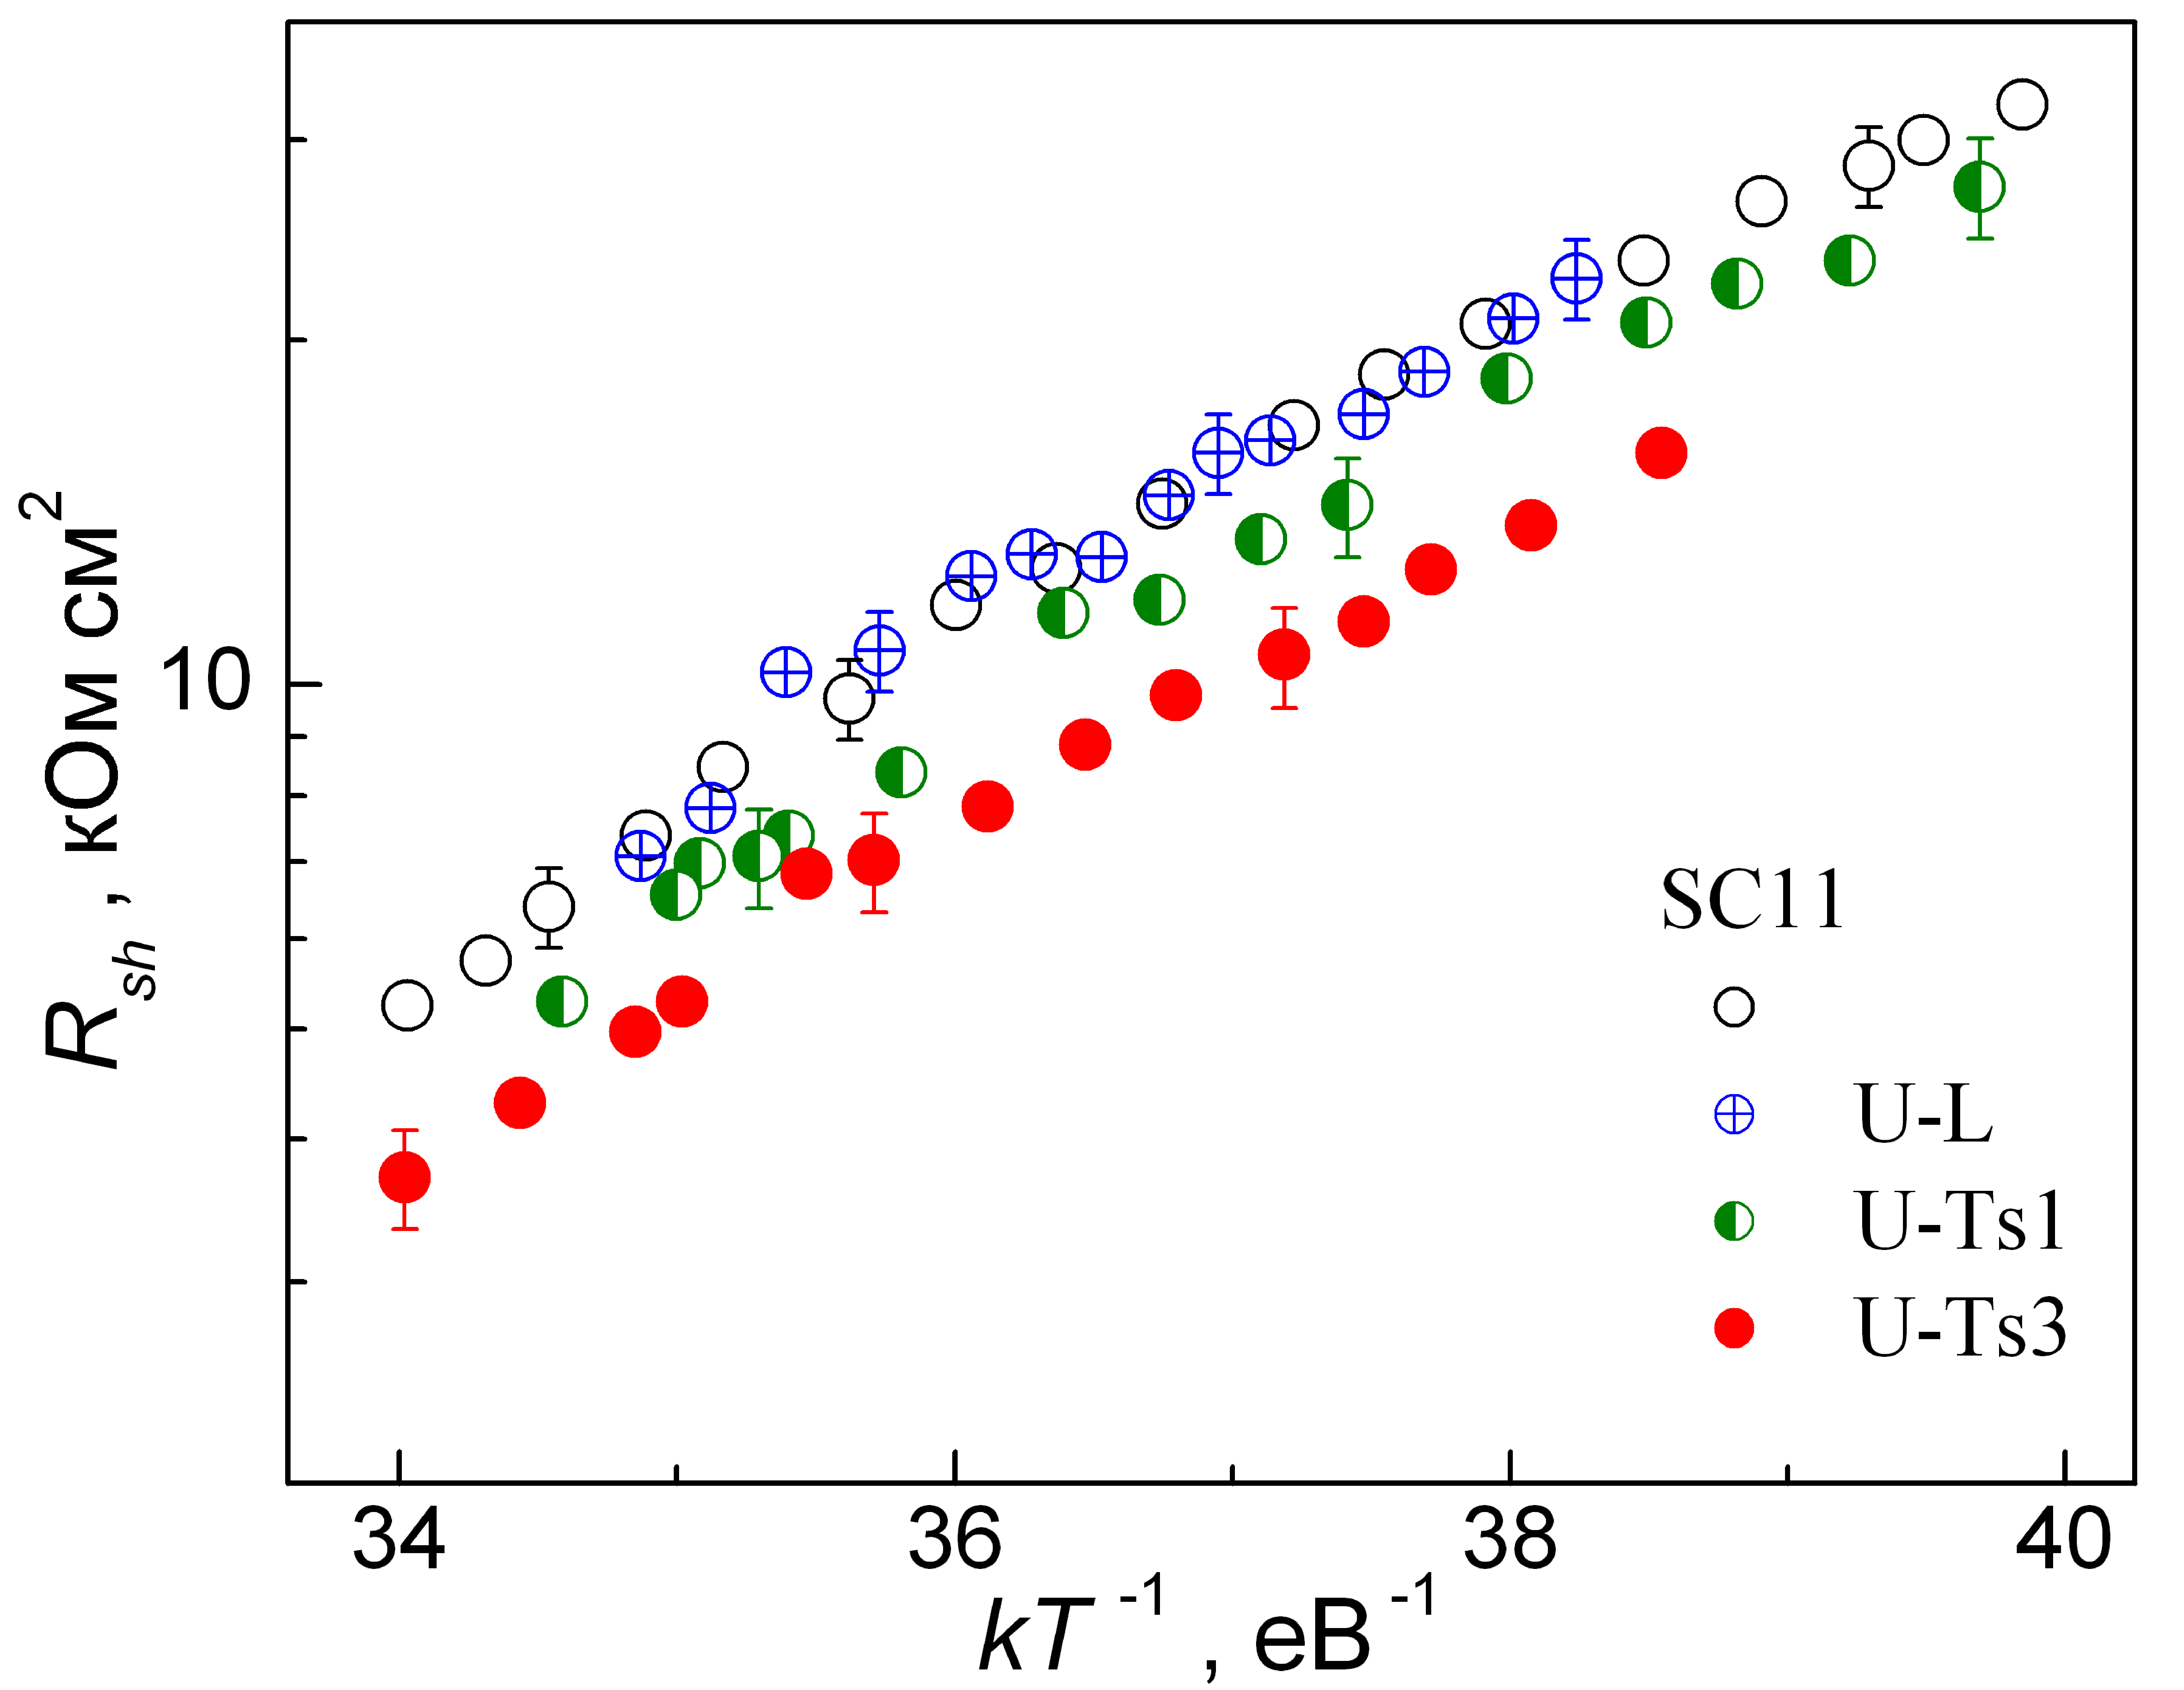
\includegraphics[width=0.7\textwidth]{figDUS_Rsh}%
\caption{\label{figDUS_Rsh}
Температурні залежності шунтуючого опору SC11, отримані за умов УЗН та без нього (порожні кола).
}%
\end{figure}

На Рис.~\ref{figDUS_Rsh} показана температурна залежність шунтуючого опору зразка SC11.
Зауважимо, що для SC17 $R_{sh}>10^{15}$~Ом$\cdot$см$^2$ незалежно від температури та УЗН і
шунтуючий опір не впливав на ВАХ.
З усього дослідженого набору зразків лише цей мав подібну особливість.
З рисунка видно, що УЗН з використанням поперечних хвиль викликає зменшення $R_{sh}$,
тоді як повздовжні хвилі практично не впливають на величину шунтуючого опору.
Розраховані величини як $R_{sh}$, так і його АІ змін наведені в Таблицях~\ref{tabSSCParam} та \ref{tabAIEfect}.
Детальний розгляд можливих причин виникнення $R_{sh}$ та впливу на нього УЗН наведено у параграфі~\ref{sbRsh}.

\subsection{Модель акусто--активного комплексного дефекту\label{sbAEDefect}}

Для пояснення взаємодії пружних хвиль з дефектами у неп'єзоелектричних кристалах
запропоновано чимало механізмів.
Зокрема вважається, що в умовах УЗН може відбуватися
\begin{enumerate}[label=\asbuk*),leftmargin=0em,itemindent=1.5em]
\item зміна заселеності коливних рівнів, зв'язаних з домішками \cite{Pavlovich};
\item зміщення домішкових атомів порівняно з їх оточенням \cite{Korotchenkov1995,MirzadeJAP2011,PELESHCHAK:UPJ2016};
\item зменшення енергії активації дифузії дефектів \cite{Krevchik};
\item локальне підвищення температури в області кластерів точкових дефектів  \cite{MirzadeJAP2005};
\item поглинання УЗ дислокаціями \cite{Davletova2008,OstrovKor92};
\end{enumerate}
тощо.
Проте повна теорія АДВ в кремнії ще не побудована, причиною чого, зокрема, є недостатня
кількість експериментальних досліджень, сфокусованих на вивчення АІ ефектів.

На нашу думку, виявлені оборотні АІ зміни рекомбінаційних параметрів КСЕ можна пояснити зміною
відстані між компонентами дефектного комплексу в умовах УЗН.
Зокрема, якщо мова йде про АІ модифікацію $n_{\mathrm{id}}$ та $\tau_g$,
то відбувається зміна відстані між донором та акцептором, які приймають участь у CDLR.

Дійсно, з літератури \cite{MirzadeJAP2011,PELESHCHAK:UPJ2016} відомо, що для сили $F_d$, яка діє на точковий дефект під час УЗН,
є справедливим вираз
\begin{equation}
\label{eqFd}
F_d=\chi\,\Delta\Omega_d\frac{\partial \xi(z,t)}{\partial z}\,,
\end{equation}
де
$\chi$ --- об'ємний модуль пружності,
$\Delta\Omega_d$ --- зміна об'єму кристалу, що припадає на один дефект
(для міжвузлових атомів та домішок заміщення з іонним радіусом, що перевищує радіус атома матриці $\Delta\Omega_d > 0$,
тоді як для вакансій та домішок заміщення з меншим іонним радіусом $\Delta\Omega_d < 0$);
$\xi$ --- деформація кристалічної ґратки;
при цьому вважається, що АХ поширюється в напрямі осі $Z$;
$\partial \xi(z,t)/\partial z\sim \xi_{\mathtt{US}}\sim u_\mathtt{US} \sim \sqrt{W_\mathtt{US}}$.
Таким чином, під час УЗН точковий дефект здійснює коливання, причому їх амплітуда та фаза визначаються як параметрами самого ТД, так і інтенсивністю АХ.


\begin{figure}
\center
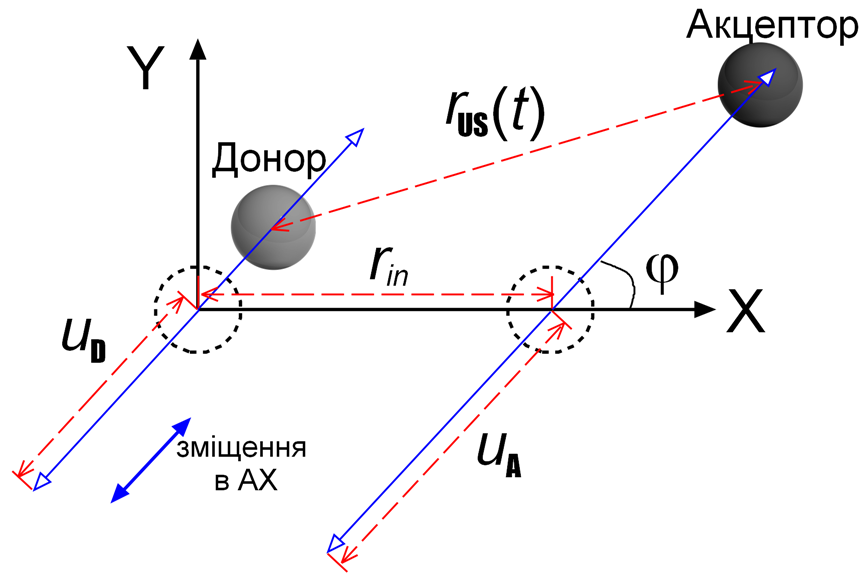
\includegraphics[width=0.7\textwidth]{fig_Model}
\caption{\label{fig_Model}
Модель поведінки дефектного комплексу в умовах УЗН.
}%
\end{figure}

На Рис.~\ref{fig_Model} показана спрощена якісна модель поведінки дефектного комплексу, який містить дві складові,
в умовах поширення АХ.
У вихідному стані, до УЗН, донор та акцептор перебувають на відстані $r_{in}$ один від одного,
вісь $X$ спрямована вздовж прямої, яка з'єднує дефекти.
В умовах УЗН дефекти коливаються з амплітудами $u_\mathtt{D}$ та $u_\mathtt{A}$.
Напрям коливань збігається з напрямом зміщень в АХ та утворює кут $\varphi$ з віссю $X$.
$u_\mathtt{D}$ та $u_\mathtt{A}$ залежать від $\xi_{U\!S}$, пружних полів дефекту (значень $\Delta\Omega_d^\mathtt{D}$ та $\Delta\Omega_d^\mathtt{A}$,
пов'язаних з кожною окремою складовою), енергії зв'язку комплексу і можуть відрізнятися між собою.
Відповідно, відстань між донором та акцептором за умов УЗН залежить від часу $t$:
\begin{multline}
\label{eqrUS}
r_\mathtt{US}(t)=\left\{[r_{in}+u_\mathtt{A}\cos(\omega_\mathtt{US}t+\delta)-u_\mathtt{D}\cos(\omega_\mathtt{US}t)]^2\cos^2\varphi \right.\\
    \left.+ [u_\mathtt{A}\cos(\omega_\mathtt{US}t+\delta)-u_\mathtt{D}\cos(\omega_\mathtt{US}t)]^2\sin^2\varphi\right\}^{0.5}\,,
\end{multline}
де
$\omega_\mathtt{US}$ --- циклічна частота УЗ, а
$\delta$ --- зсув фаз між коливаннями донора та акцептора.

Зміна відстані між компонентами комплексу, згідно з моделлю CDLR, має викликати зміни
ППЗ носіїв та величини $R_\mathtt{DA}$.
Використовуючи формули (\ref{eqSigma}) and (\ref{eqRda}), були проведені розрахунки
АІ відносних змін поперечного перерізу захоплення
$\varepsilon_\sigma=[\sigma_{\mathtt{US}}-\sigma(r_{in})]/\sigma(r_{in})$
та параметру зв'язку
$\varepsilon_{\mathtt{RDA}}=[R_{\mathtt{DA,US}}-R_\mathtt{DA}(r_{in})]/R_\mathtt{DA}(r_{in})$,
де $\sigma_{\mathtt{US}}$ та $R_{\mathtt{DA,US}}$ були усереднені по періоду АХ $T_\mathtt{US}$:
\begin{equation}
\label{eqAverSigma}
\sigma_{\mathtt{US}}=\frac{1}{T_\mathtt{US}}\int^{T_\mathtt{US}}_0\!\!\!\!\!\!\sigma(r_\mathtt{US}(t))dt\,,
\end{equation}
\begin{equation}
\label{eqAverRda}
R_{\mathtt{DA,US}}=\frac{1}{T_\mathtt{US}}\int^{T_\mathtt{US}}_0\!\!\!\!\!\!R_{\mathtt{DA}}(r_\mathtt{US}(t))dt\,.
\end{equation}


\begin{figure}
\center
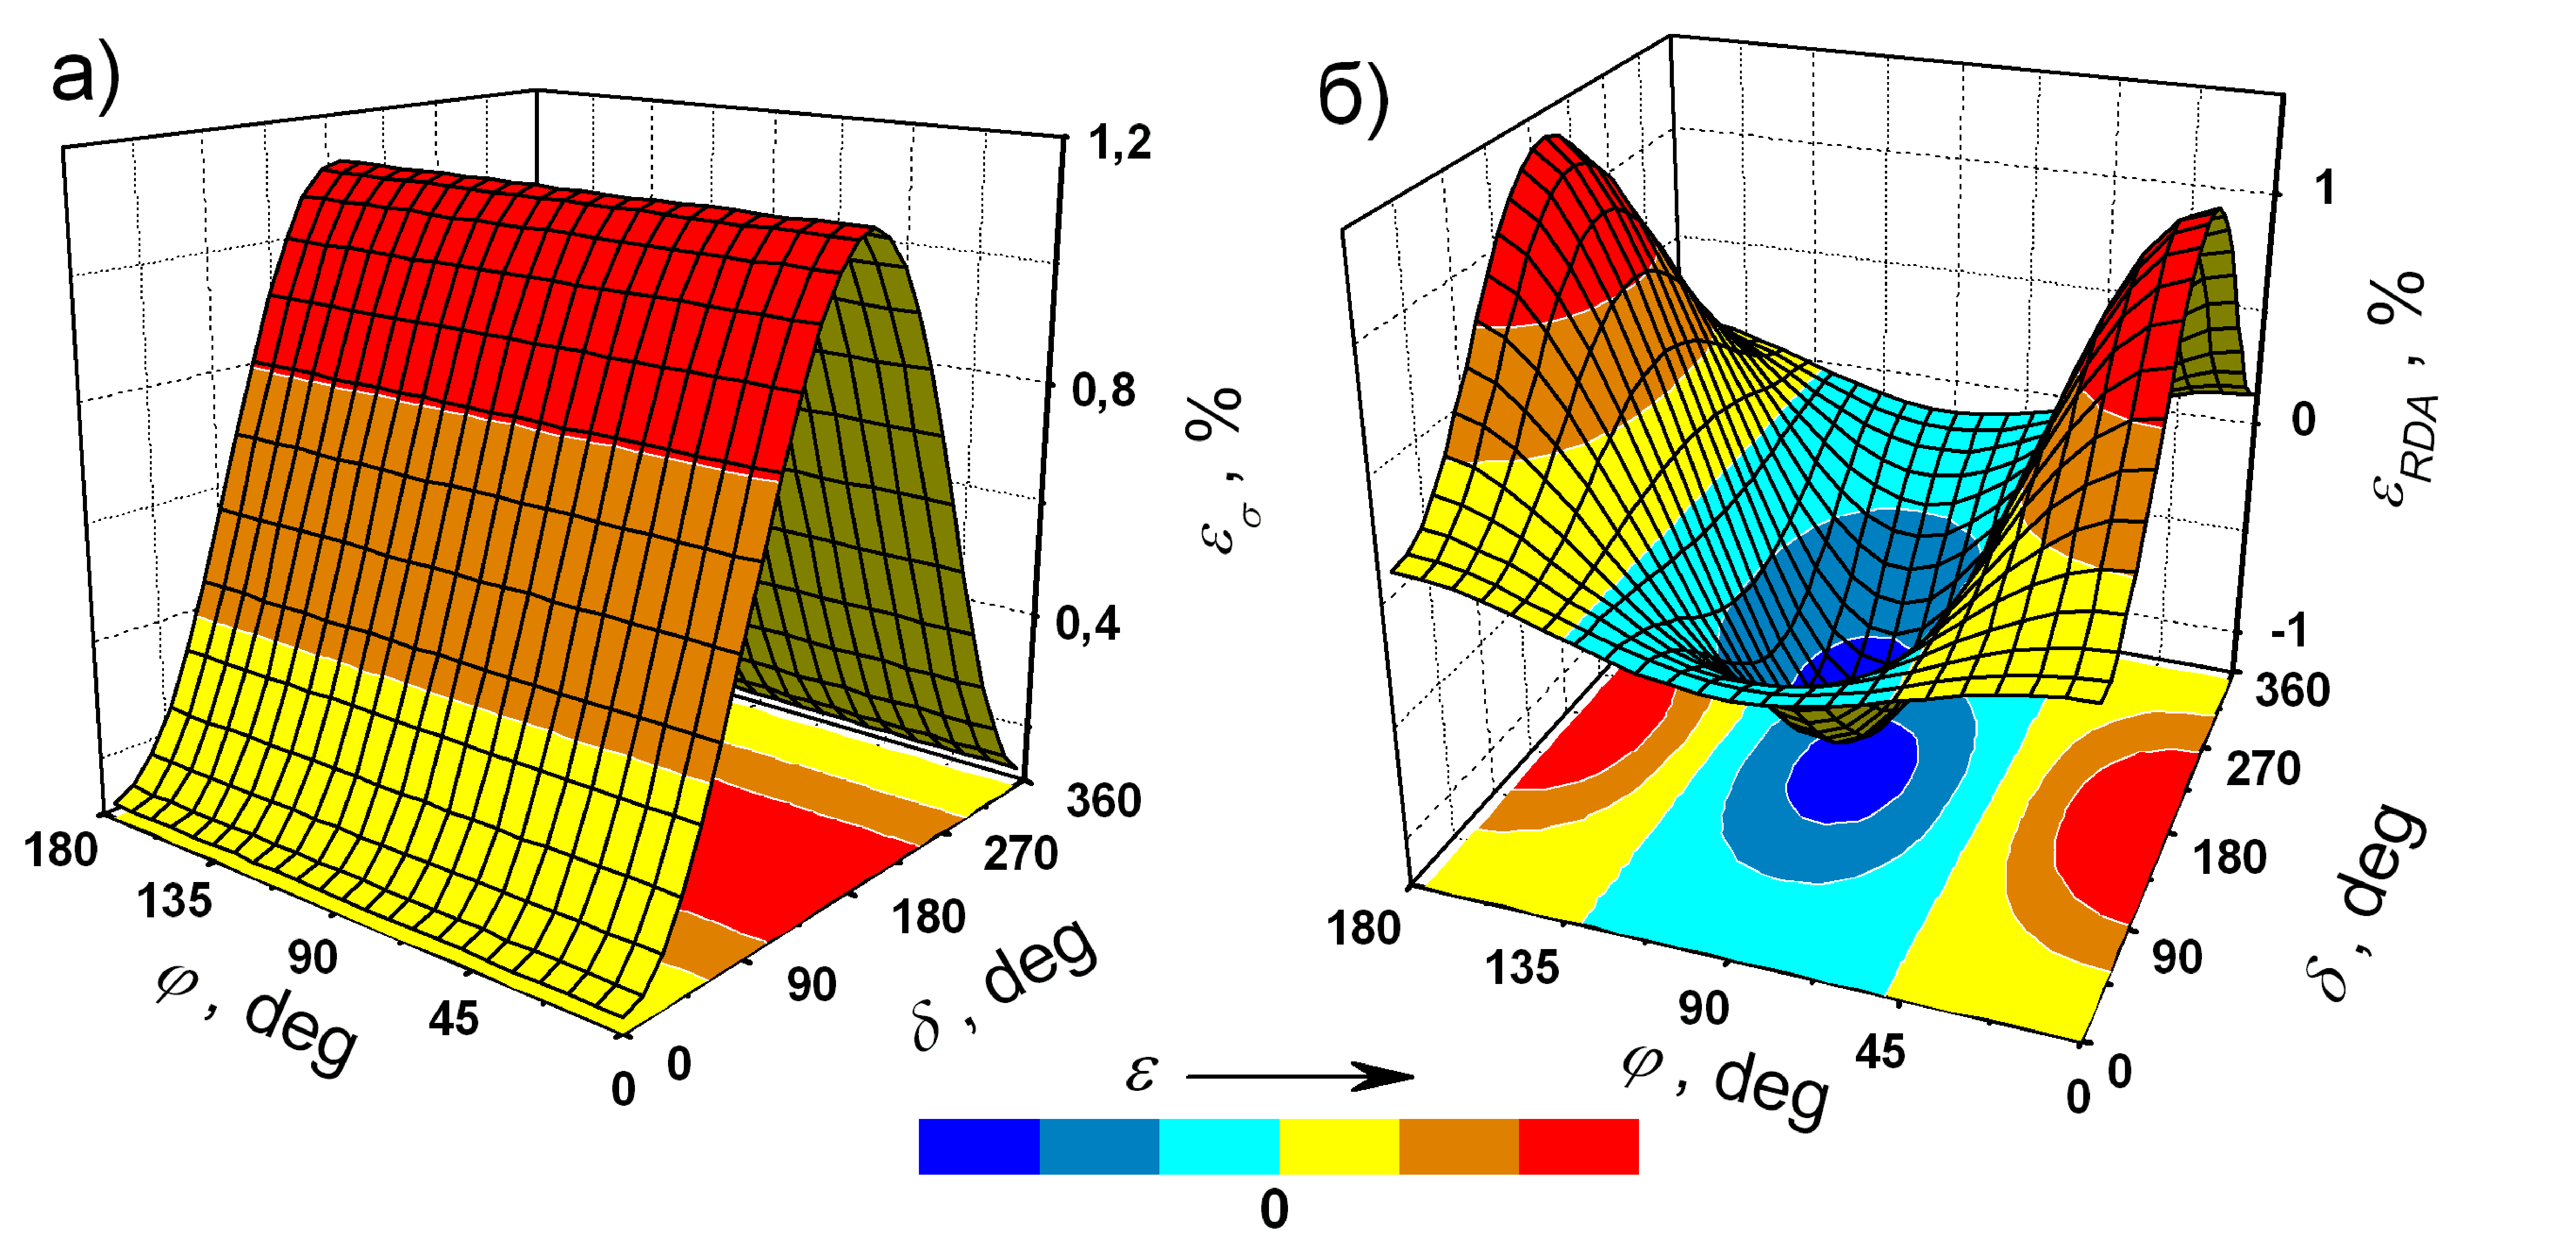
\includegraphics[width=0.95\textwidth]{figR2L}
\caption{\label{figR2L}
Розраховані залежності  АІ змін поперечного перерізу захоплення носіїв (а) та параметру зв'язку (б) від зсуву фаз між коливаннями та від взаємного
розташування вісі комплексу та напряму зміщень в АХ.
При розрахунках вважалося, що $a_B=3.23$~нм, $r_{in}=10$~нм, $u_A=1$~нм та $u_D=0.5$~нм.
}%
\end{figure}

\begin{figure}
\center
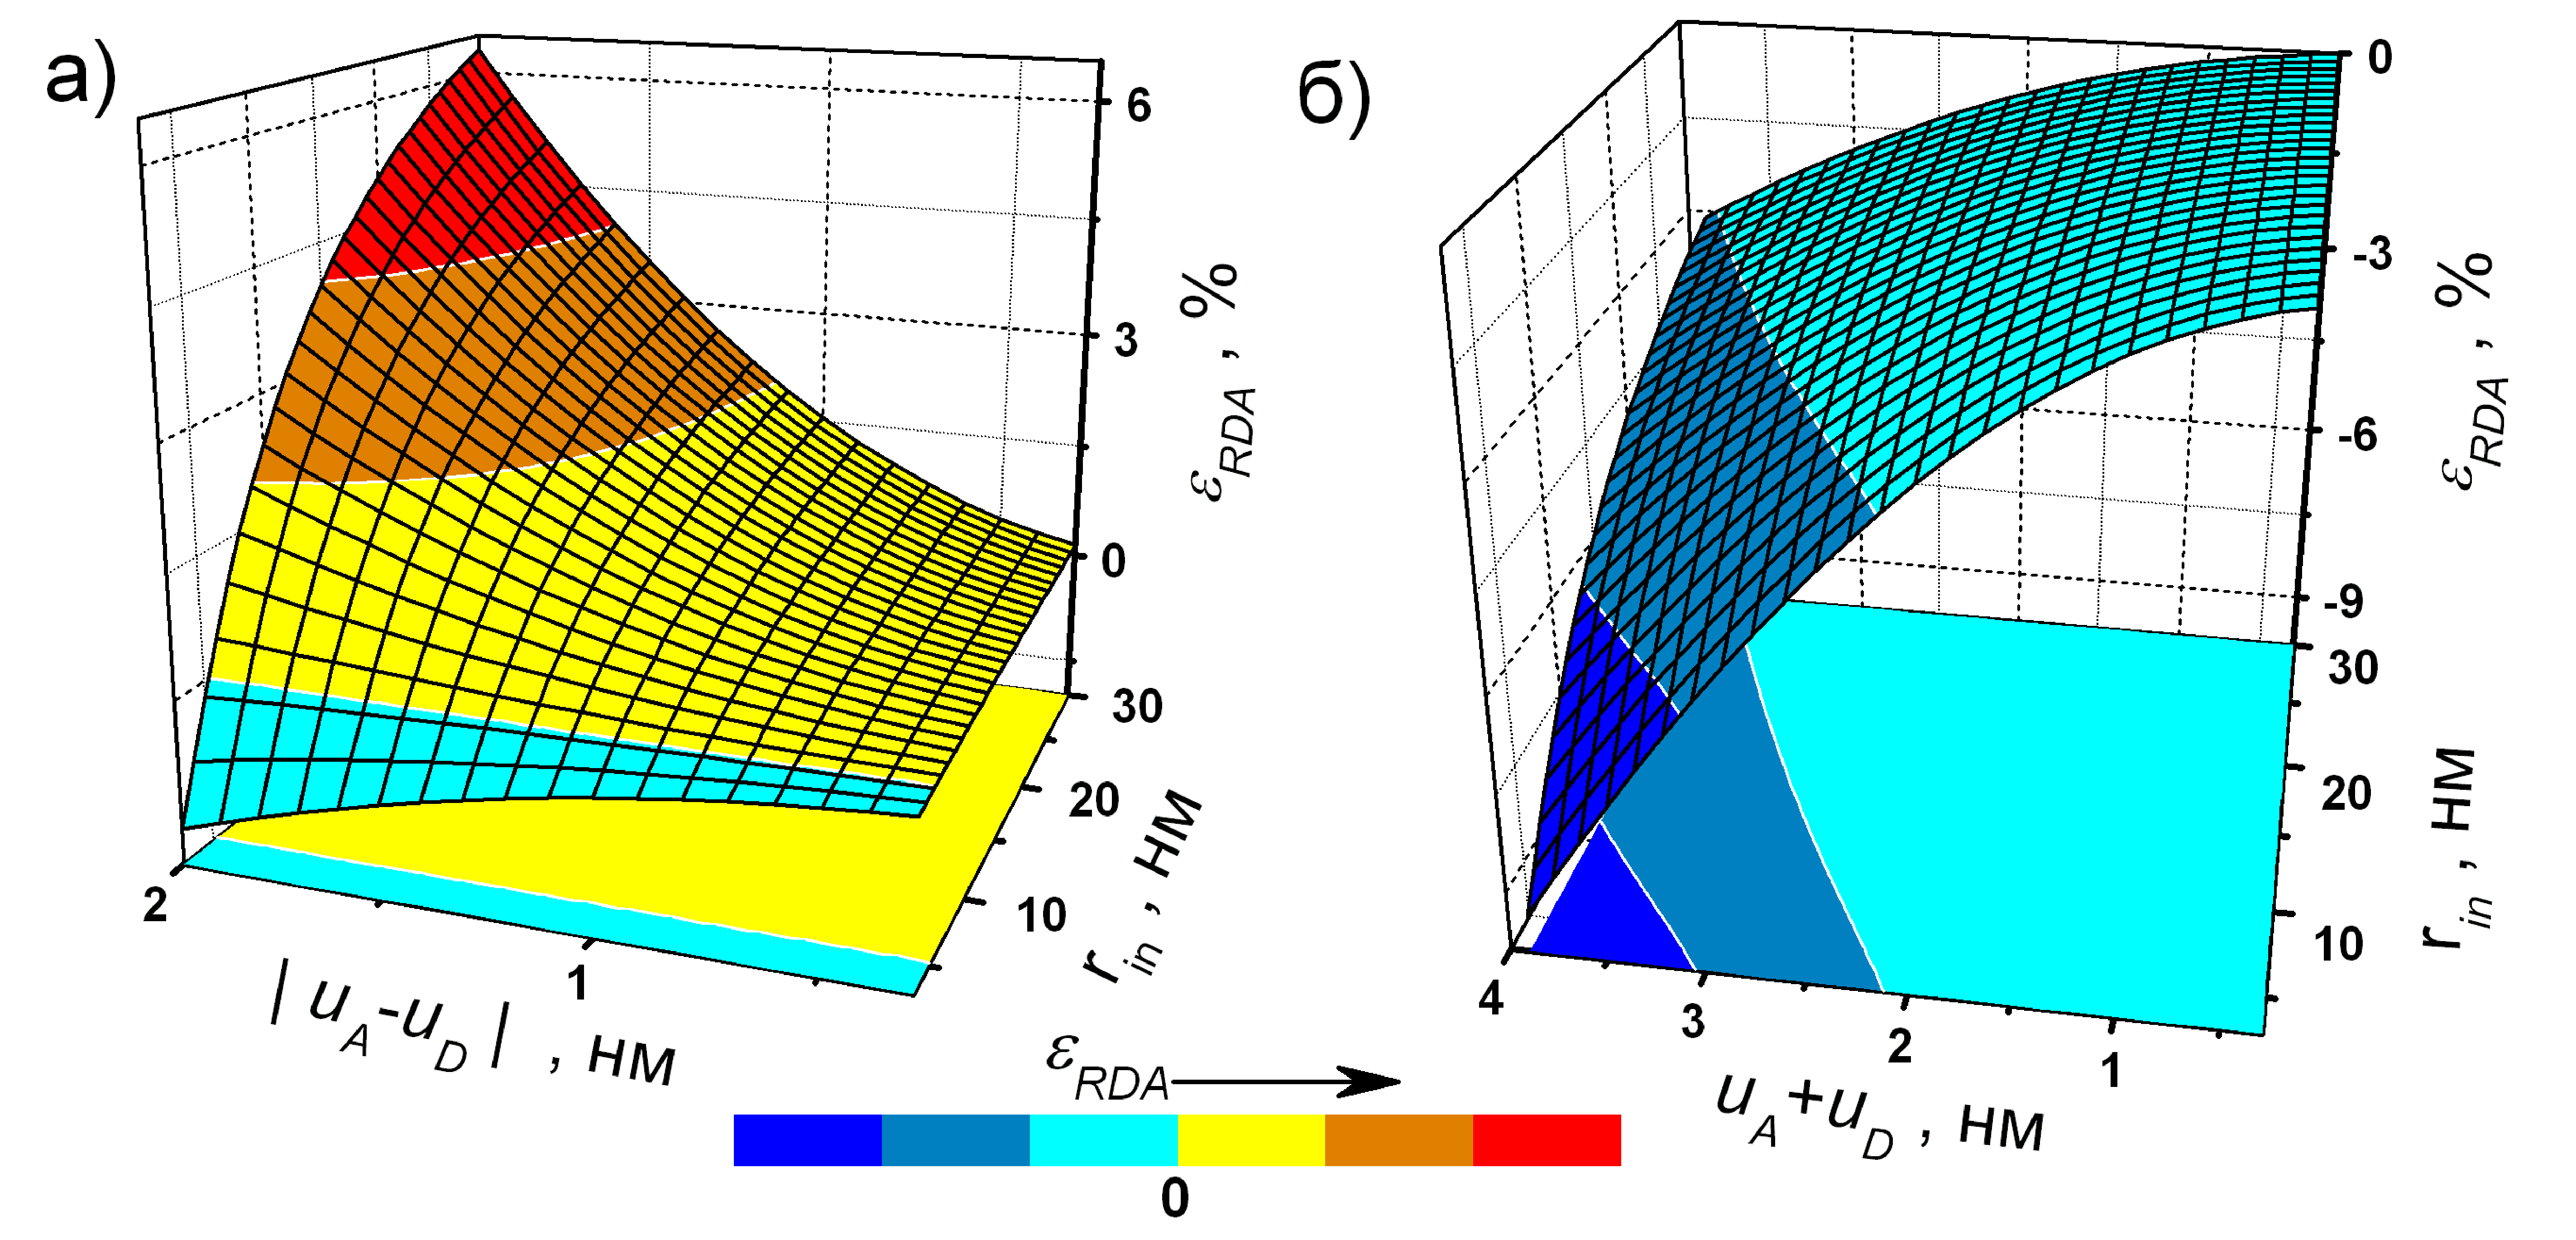
\includegraphics[width=0.95\textwidth]{figLnew}
\caption{\label{figLnew}
Розраховані залежності  АІ змін параметру зв'язку від амплітуди коливань та початкової відстані між компонентами.
При розрахунках вважалося, що $\varphi=0^\circ$, $\delta=0^\circ$ (a) та $\varphi=90^\circ$, $\delta=180^\circ$ (б).
}%
\end{figure}

Декілька типових прикладів результатів розрахунків показано на Рис.~\ref{figR2L} та Рис.~\ref{figLnew}.
Під час їх проведення вважалося, що
\begin{enumerate}[label=\asbuk*),leftmargin=0em,itemindent=1.5em]
\item характерний час релаксації в CDLR--підсистемі набагато менший, ніж $T_\mathtt{US}$;
\item $a_B=3.23$~нм ---значення, яке раніше використовувалося в літературі \cite{CDLR:JAP};
\item значення $u_\mathtt{D}$ та $u_\mathtt{A}$ співрозмірні з $u_\mathtt{US}$;
   проте при цьому потрібно взяти до уваги, що зміщення домішкових атомів, які не утворюють ковалентних зв'язків з оточенням, може перевищувати
   зміщення атомів, які утворюють кристалічну ґратку.
\end{enumerate}

Додатковою причиною зміни відстані між компонентами комплексу може бути постійна механічна напруга,
яка виникає при поширенні АХ у кристалі.
Цей ефект спочатку був передбачений теоретично \cite{Thurston,StaticStrain:PhysRevB30I}, а потім
спостережений експериментально, зокрема у кремнії \cite{StaticStrain:PhysRevB30II}.
Величина додаткового тиску пропорційна квадрату частоти УЗ, квадрату зміщень у хвилі та коефіцієнту нелінійності\cite{StaticStrain:PhysRevB30II}.
Коефіцієнт нелінійності анізотропний, зокрема для Si при
поширенні УЗ вздовж напрямку [111] його величина займає проміжне положення між значеннями, характерними для розповсюдження АХ
паралельно напрямам [100] та [110] \cite{NelinSi}.
Крім того, для кремнію коефіцієнт нелінійності додатній, що викликає розтяг кристалу при УЗН.



%при поширенні акустичної хвилі в кристалі (в тому числі і кремнії) виникає  постійна механічна напруга,
%яка приводить до розтягу твердого тіла (якщо коефіцієнт акустичної нелінійності додатній, як в кремнії)
%ефект передбачено теоретично \cite{Thurston,StaticStrain:PhysRevB30I}
%спостережено експериментально в кремнії \cite{StaticStrain:PhysRevB30II}
%величина додаткового тиску пропорційна квадрату частоти УЗ, квадрату зміщень в хвилі та коефіцієнту нелінійності\cite{StaticStrain:PhysRevB30II}
%величина коефіцієнту нелінійності залежить від напрямку поширення хвилі:
%для [100] --- 2.0, [110] --- 4.7, [111] --- 3.8 \cite{NelinSi}
%про повздовжні/поперечні хвилі не знайшов.. може погано шукав...

Як видно з Рис.~\ref{figR2L},a, УЗН викликає збільшення ППЗ.
Залежності АІ змін параметру зв'язку більш складні і не монотонні -- див. Рис.Fig.~\ref{figR2L},б.
Зокрема, очікується  зменшення $R_{\mathtt{DA}}$ якщо $\varphi\approx90^\circ$ (тобто вісь комплексу перпендикулярна до напрямку зміщень в АХ, див. Рис.~\ref{figLnew},б)
або при малих значеннях $r_{in}/a_B$ (див. Рис.~\ref{figLnew},а).
До речі, в останньому випадку передбачається \cite{CDLR:JAP1995,CDLR:JAP}, що процеси CDLR будуть відбуватися найбільш інтенсивно.

У спрощеному випадку незначної дисипації енергії пружних коливань на дефектах
%Якщо припустити, що на дефектах не відбувається дисипація енергії УЗ, то в такому спрощеному випадку
$\delta$ може бути рівним або $0^\circ$ (якщо $(\Delta\Omega_d^\mathtt{D}\cdot\Delta\Omega_d^\mathtt{A})>0$)
або $180^\circ$ (якщо $(\Delta\Omega_d^\mathtt{D}\cdot\Delta\Omega_d^\mathtt{A})<0$).
Виявляється, що при цьому величина $\varepsilon_{\mathtt{RDA}}$ не залежить від абсолютних значень $u_\mathtt{A}$ та $u_\mathtt{D}$,
а визначається лише їх сумою $|u_\mathtt{D}+u_\mathtt{A}|$ (при $\delta=180^\circ$)
або модулем їх різниці $|u_\mathtt{D}-u_\mathtt{A}|$ (при $\delta=0^\circ$).
Більше того, ці залежності (від $|u_\mathtt{D}+u_\mathtt{A}|$ або від $|u_\mathtt{D}-u_\mathtt{A}|$) однакові в обох випадках
(при $\delta=180^\circ$ і при $\delta=0^\circ$).
Декілька прикладів таких розрахованих залежностей наведено на Рис.~\ref{fig_Erda}.

\begin{figure}
\center
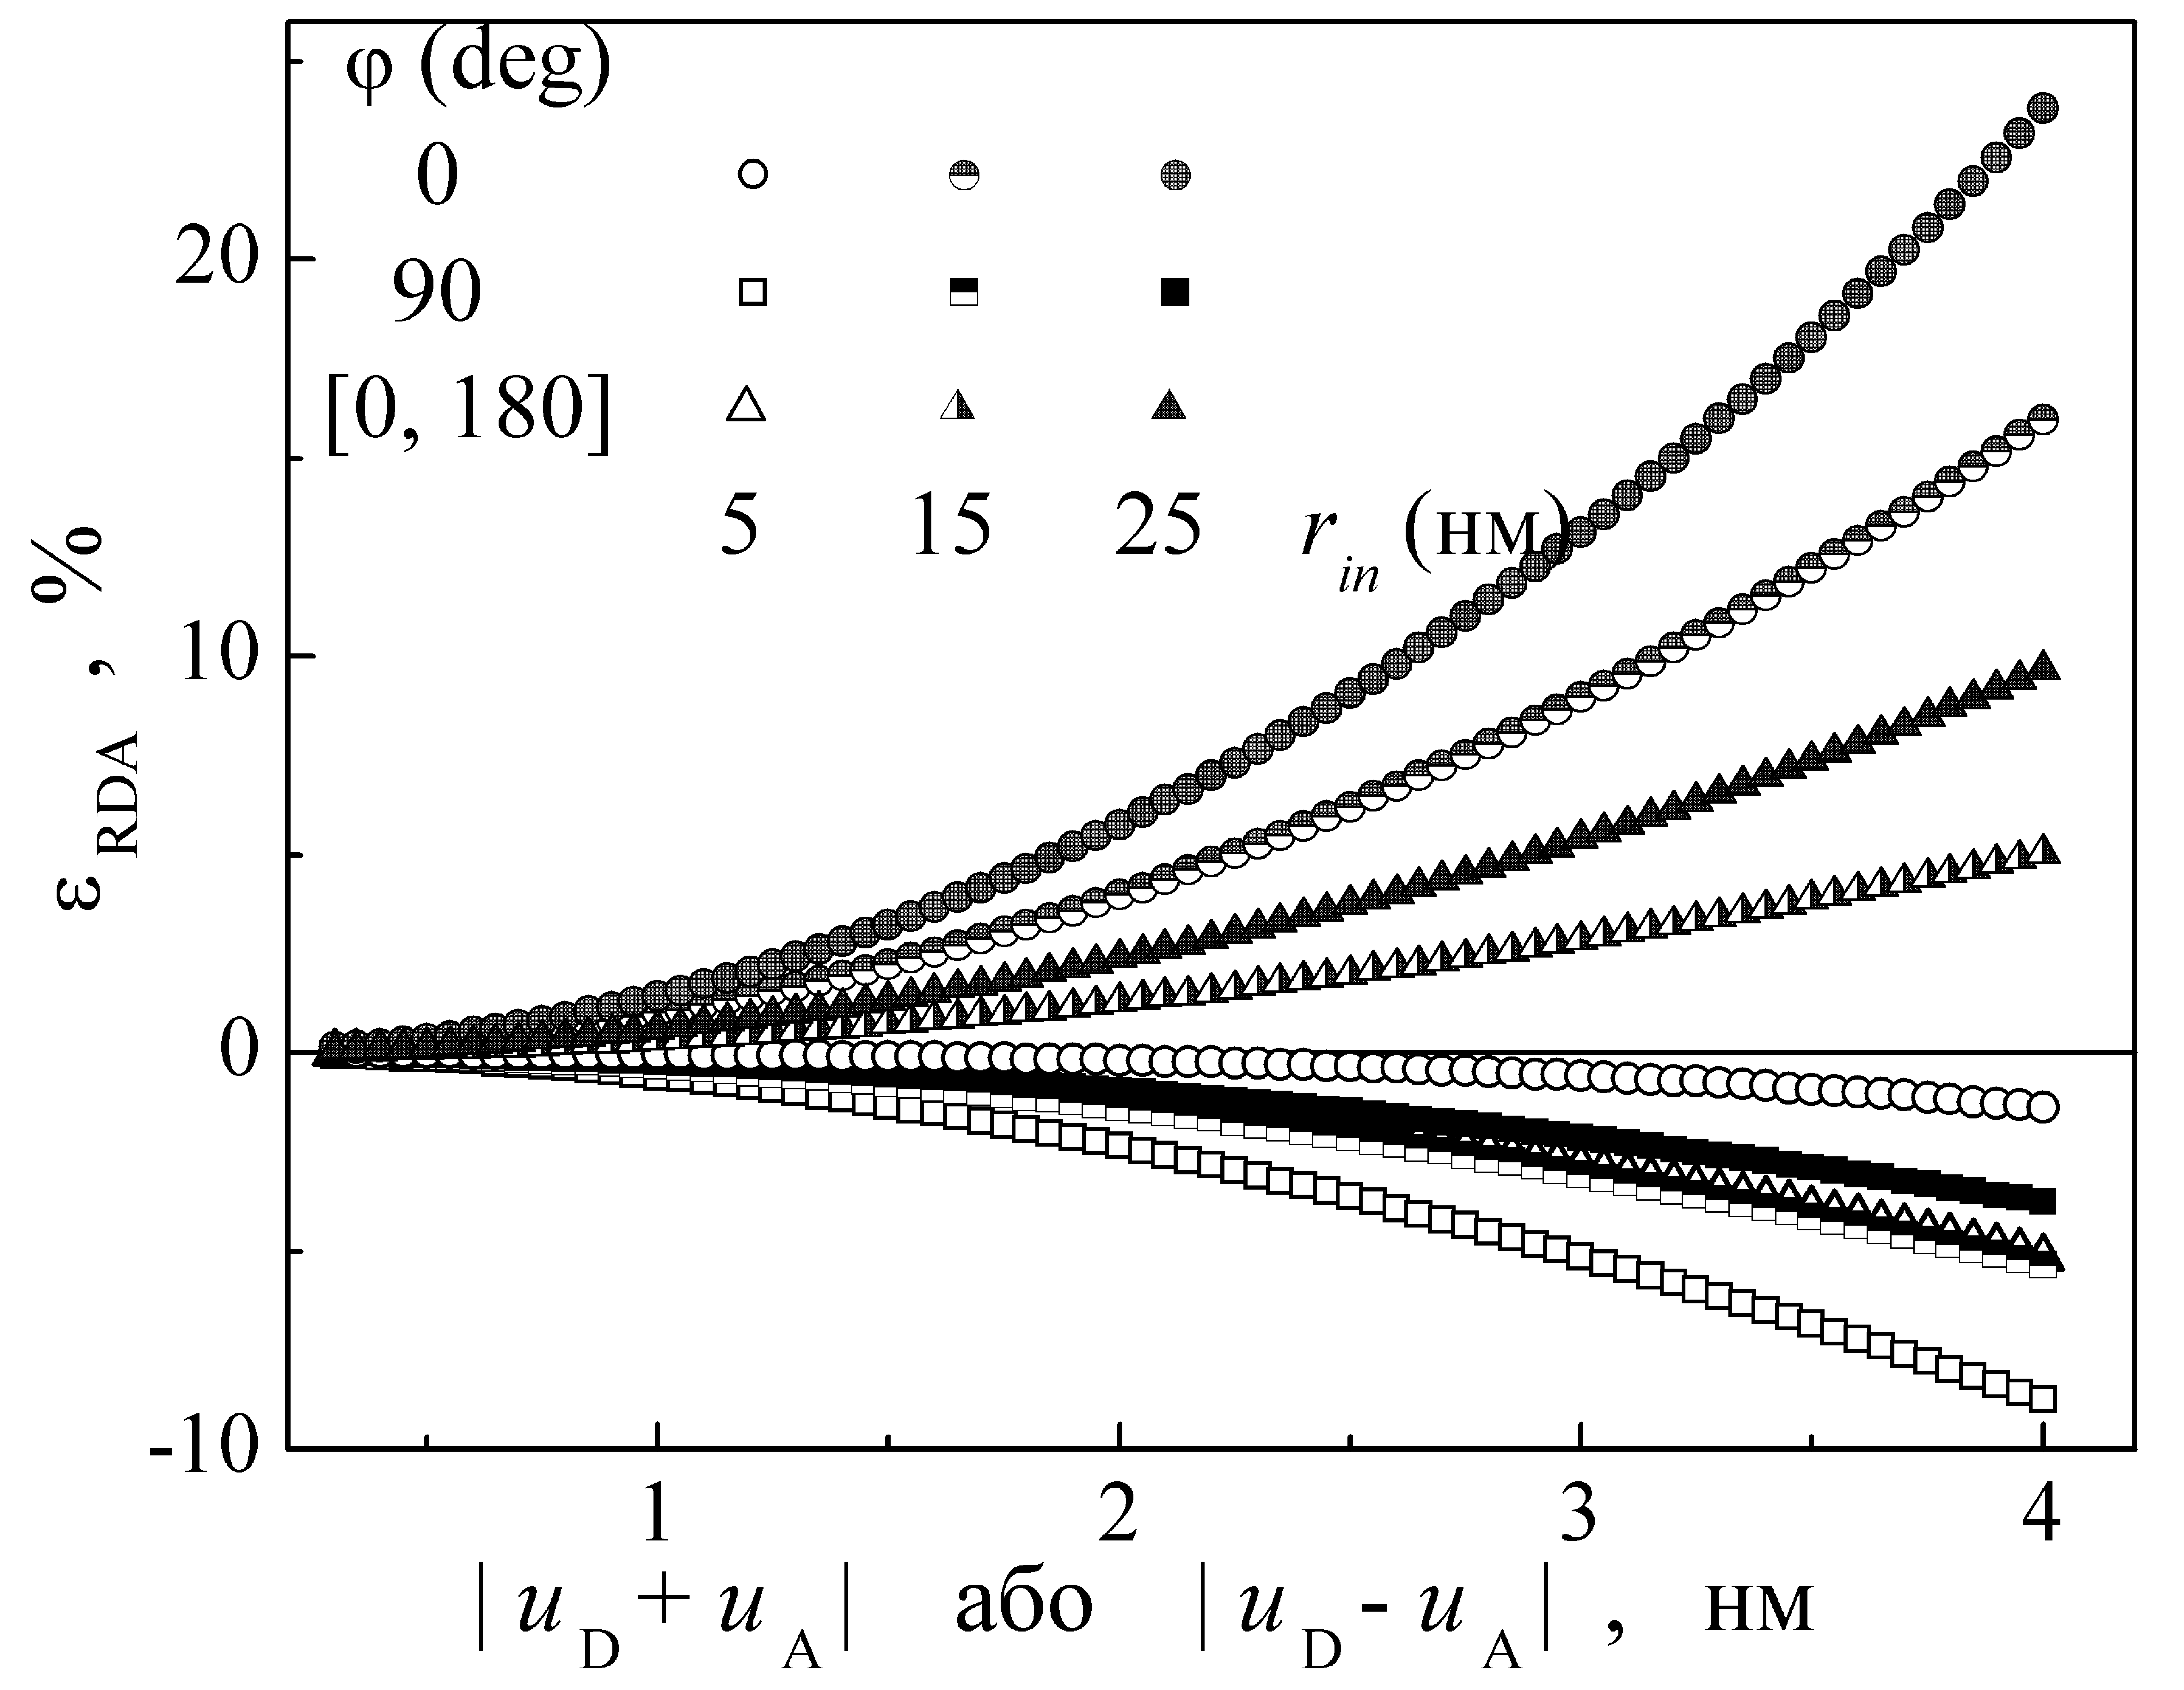
\includegraphics[width=0.75\textwidth]{fig_Erda}
\caption{\label{fig_Erda}
Розраховані залежності АІ змін параметру зв'язку від амплітуди коливань.
По горизонталі відкладено $|u_\mathtt{D}-u_\mathtt{A}|$ для випадків $\delta=0^\circ$ та
$|u_\mathtt{D}+u_\mathtt{A}|$ при $\delta=180^\circ$.
При розрахунках вважалося, що
$a_B=3.23$~нм,
$r_{in}=5$~нм (незаповнені точки), $15$~нм (напівзаповнені точки) та $25$~нм (заповнені точки),
$\varphi=0^\circ$ (кола), $90^\circ$ (квадрати).
Трикутники відповідають середнім значенням $\varepsilon_{\mathtt{RDA}}$,
обчисленим для діапазону $\varphi$ від $[0^\circ$ до $180^\circ]$.
}%
\end{figure}

Залежність відносної зміни ППЗ від амплітуди коливань має подібний характер, більше того
вона не залежить від $\varphi$:
\begin{equation}
\label{eqEpsSig}
\varepsilon_{\sigma}=\frac{(u_\mathtt{D}\pm u_\mathtt{A})^2}{2\,r_{in}^2}\,,
\end{equation}
де
знаки <<$+$>> та <<$-$>> відповідають випадкам $\delta=180^\circ$ та $\delta=0^\circ$, відповідно.
Тобто, при $(\Delta\Omega_d^\mathtt{D}\cdot\Delta\Omega_d^\mathtt{A}<0)$ ефективність впливу УЗ має бути більшою,
так як в цьому випадку вона визначається сумою зміщень компонент пари,
тоді як в протилежному --- їх різницею


Враховуючи, що $u_\mathtt{D},u_\mathtt{A}\sim \xi_\mathtt{US}\sim u_\mathtt{US}\sim \sqrt{W_\mathtt{US}}$,
остання формула може бути записана у вигляді
\begin{equation}
\label{eqEpsSigUS}
\varepsilon_{\sigma}=K_\mathtt{US}^\mathtt{DA}\,\,u_{\mathtt{US}}^2=K_\mathtt{US}^\mathtt{DA*}\,\,W_{\mathtt{US}}\,,
\end{equation}
де $K_\mathtt{US}^\mathtt{DA}$ ($K_\mathtt{US}^\mathtt{DA*}$) характеризує взаємодію УЗ з парою донор--акцептор
та залежить від властивостей дефектів та кристалічної ґратки (і ще й від типу хвиль для $K_\mathtt{US}^\mathtt{DA*}$).

Звичайно, можлива орієнтація пари зумовлена мінімізацією її повної енергії, а отже існують визначається кристалографічними осями.
Проте, з одного боку, врахуємо що кристали кремнію характеризуються кубічною симетрією і містять достатньо велику кількість еквівалентних напрямів.
З  іншого боку, необхідно врахувати,
що струм, пов'язаний з CDLR процесами протікає переважно в околі протяжних дефектів \cite{CDLR:JAP,CDLR:SSP}.
Нарешті, дислокації в ОПЗ нерідко розташовуються перпендикулярно площині $p-n$ переходу
і досліджені структури не є винятком (див. параграф~\ref{sbRsh}).
Якщо дефектна пара та дислокація розташовані поблизу один одного, то дислокація з крайовою компонентою буде впливати на просторове розташування пари.
Як наслідок, у ідеальному випадку пара донор--акцептор з  $(\Delta\Omega_d^\mathtt{D}\cdot\Delta\Omega_d^\mathtt{A}>0)$ переважно будуть орієнтовані
паралельно дислокаційній лінії,
тоді як вісь спарених дефектів з $(\Delta\Omega_d^\mathtt{D}\cdot\Delta\Omega_d^\mathtt{A}<0)$ має утворювати з дислокаційною лінією прямий кут.
При цьому, при поширенні УЗ перпендикулярно площині $p-n$ переходу (як в експериментах)
%використанні поперечних хвиль (зміщення паралельні площині $p-n$ переходу)
найбільш цікавими будуть наступні випадки

\noindent при  $\delta=0^\circ$ (випадок $\Delta\Omega_d^\mathtt{D}\cdot\Delta\Omega_d^\mathtt{A}>0$):
\begin{center}
\noindent   $\varphi=90^\circ$ (поперечні хвилі)  та $\varphi=0^\circ$ (повздовжні хвилі)
\end{center}

\noindent при  $\delta=180^\circ$ (випадок $\Delta\Omega_d^\mathtt{D}\cdot\Delta\Omega_d^\mathtt{A}<0$):
\begin{center}
\noindent   $\varphi\in[0^\circ\div 180^\circ]$ (поперечні хвилі)  та $\varphi=90^\circ$ (повздовжні хвилі).
\end{center}

Іншими словами,
якщо зміна об'єму кристалу, пов'язана з донором, протилежна за знаком зміні об'єму кристалу, пов'язаній з акцептором, то
при поширенні поперечних хвиль можуть реалізуватися випадки, які відповідають всім кривим на Рис.~\ref{fig_Erda}.
Якщо ж $\Delta\Omega_d^\mathtt{D}\cdot\Delta\Omega_d^\mathtt{A}>0$, то потрібно брати до уваги лише криві, для позначення
яких використано квадрати.


Таким чином, в рамках запропонованої моделі очікується, що УЗН спричинює зміну відстані між донором та акцептором,
що стає причиною появи $\varepsilon_{\sigma}$ та $\varepsilon_{\mathtt{RDA}}$, величина яких переважно визначається АІ зміщенням атомів.
Згідно з CDLR теорією,
збільшення ППЗ та зменшення параметру зв'язку має викликати зменшення часу життя носіїв та збільшення фактору неідеальності,
що і спостерігається на експерименті.


Запропонована модель може бути використана і для пояснень впливу УЗ на процеси рекомбінації в КНО (див. Рис.~\ref{figDUSTau}).
Так як АІ зміни оборотні, то зміна часу життя, згідно з (\ref{eqTAUSHRsum}), може бути пов'язана лише зі збільшенням
$\sigma_n$ в умовах УЗН.
Відомо, що переважна більшість рекомбінаційних центрів у кремнії є комплексними ТД,
причому компоненти комплексу не еквівалентні між собою.
Зокрема, нерідко вони характеризуються протилежним електричним зарядом.
В літературі \cite{CDLR:R2} запропоновано, що для подібних ТД також має виконуватись емпіричне співвідношення~(\ref{eqSigma}),
причому в такому випадку $r$ визначається відстанню між компонентами комплексного ТД, яка  менша, ніж відстань між донором та акцептором в CDLR.
В цьому випадку, згідно з описаною моделлю, УЗН також викликає зміну $r$ та $\sigma_n$ відповідно до виразу (\ref{eqEpsSigUS}).
Проте якщо для випадку CDLR зміна ППЗ носіїв донором (і/або акцептором) доповнюється зміною параметру зв'язку,
то при АІ варіація часу життя в КНО визначається лише модифікацією поперечного перерізу захоплення.

Ефективність АДВ залежить від типу дефекту та його структури \cite{UST:Medvid}
і не всі дефекти в кремнії є акусто активними (ААД).
Якщо $M_d^\mathtt{AA}$ та $M_d^\mathtt{nonAA}$ --- загальна кількість типів ААД та не акусто активних (non--AA) центрів,
то вираз (\ref{eqTAUSHRsum}) для $\tau_{n}^{-1}$ в умовах УЗН та без нього може бути записаний у вигляді
\begin{eqnarray}
\tau_{n,in}^{-1}&=&\sum_j^{M_d^\mathtt{AA}}N_{d,j}\,\sigma_{n,j}^{in}\,\upsilon_{\mathrm{th},n}+
\sum_l^{M_d^\mathtt{nonAA}}N_{d,l}\,\sigma_{n,l}\,\upsilon_{\mathrm{th},n}\,,\\
\tau_{n,\mathtt{US}}^{-1}&=&\sum_j^{M_d^\mathtt{AA}}N_{d,j}\,\sigma_{n,j}^\mathtt{US}\,\upsilon_{\mathrm{th},n}+
\sum_l^{M_d^\mathtt{nonAA}}N_{d,l}\,\sigma_{n,l}\,\upsilon_{\mathrm{th},n}\,.
\end{eqnarray}
Враховуючи, що $\sigma_{n,j}^\mathtt{US}=(\varepsilon_{\sigma,j}+1)\sigma_{n,j}^{in}$ останнє співвідношення може бути записано
у вигляді
\begin{eqnarray}
\label{eqEpsSigUSA}
\tau_{n,\mathtt{US}}^{-1}&=&\sum_j^{M_d^\mathtt{AA}}N_{d,j}\,\sigma_{n,j}^{in}\,\upsilon_{\mathrm{th},n}+
\sum_j^{M_d^\mathtt{AA}}N_{d,j}\,\sigma_{n,j}^{in}\,\varepsilon_{\sigma,j}\,\upsilon_{\mathrm{th},n}+
\sum_l^{M_d^\mathtt{nonAA}}N_{d,l}\,\sigma_{n,l}\,\upsilon_{\mathrm{th},n}=\nonumber\\
&=&\tau_{n,in}^{-1}+\sum_j^{M_d^\mathtt{AA}}N_{d,j}\,\sigma_{n,j}^{in}\,\varepsilon_{\sigma,j}\,\upsilon_{\mathrm{th},n}\,.
\end{eqnarray}
Взявши до уваги (\ref{eqEpsSigUS}), отримуємо
\begin{eqnarray}
\tau_{n,\mathtt{US}}^{-1}&=&\tau_{n,in}^{-1}+
\sum_j^{M_d^\mathtt{AA}}N_{d,j}\,\sigma_{n,j}^{in}\,K_\mathtt{US,j}\,\,u_{\mathtt{US}}^2\,\upsilon_{\mathrm{th},n}=\nonumber\\
&=&\tau_{n,in}^{-1}+u_{\mathtt{US}}^2\,\sum_j^{M_d^\mathtt{AA}}N_{d,j}\,\sigma_{n,j}^{in}\,K_\mathtt{US,j}\,\upsilon_{\mathrm{th},n}\,,
\end{eqnarray}
де $K_\mathtt{US,j}$ описує взаємодію УЗ з дефектом $j$--го типу.
Порівнявши з (\ref{eqMS_Us}) можемо сказати, що параметр $K_\mathtt{US}$, який кількісно описує експериментально виявлений вплив УЗ на час життя неосновних носіїв в базі КСЕ,
залежить від кількості АА дефектів та їх концентрації:
\begin{equation}
\label{eqKUS}
K_\mathtt{US}=\sum_j^{M_d^\mathtt{AA}}N_{d,j}\,\sigma_{n,j}^{in}\,K_\mathtt{US,j}\,\upsilon_{\mathrm{th},n}=\sum_j^{M_d^\mathtt{AA}}\frac{K_\mathtt{US,j}}{\tau_{n,j}^{in}}\,.
\end{equation}
Більше значення $K_\mathtt{US}$, отримане для SC17 (див. Таблицю~\ref{tabSSCParam}), свідчить про наявність у цьому зразку більшої кількості ААД та/або більшої їх концентрації.

Виявлена лінійність залежності зворотного часу життя від амплітуди атомних зміщень (див. Рис.~\ref{figKus},б) підтверджує
справедливість запропонованої моделі.
Крім того, зауважимо що так як початкова відстані $r_{in}$ між компонентами комплексного ТД, яка  менша, ніж початкова відстань між донором та акцептором в CDLR,
то, згідно з формулою~(\ref{eqEpsSig}), очікується що УЗ має більш ефективно впливати в першому випадку.
Саме таке співвідношення ($\varepsilon_{\tau n}>\varepsilon_{\tau g}$) і спостерігається на експерименті --- див. Таблицю~\ref{tabAIEfect}.


\subsection{Чисельний розрахунок залежностей напруги холостого ходу та фактора форми\label{sbVocSim}}

Як вже згадувалося раніше,
аналітичні вирази, які б відображали залежність напруги холостого ходу та фактора форми сонячного елементу
від $\tau_g$, $\tau_n$, $n_{\mathrm{id}}$ та $R_{sh}$ в рамках  моделі подвійного діода відсутні.
З метою візуалізації подібних залежностей були проведені чисельні розрахунки.
Вони полягали в тому, то використовуючи
формули (\ref{eqSSCIV})--(\ref{eqAlpha}) був синтезований набір ВАХ, які відповідали різним
значенням параметрів.
При цьому використовувалися значення параметрів, що були близькі до тих, якими характеризувалися досліджені КСЕ.
Після цього з штучних ВАХ використовуючи традиційний спосіб були визначені $V_{oc}$ та $F\!F$.
Типові приклади результатів обчислень, які відповідають температурі 320~K, наведено на Рис.~\ref{figVoc} та Рис.~\ref{figFF}.


\begin{figure}
\center
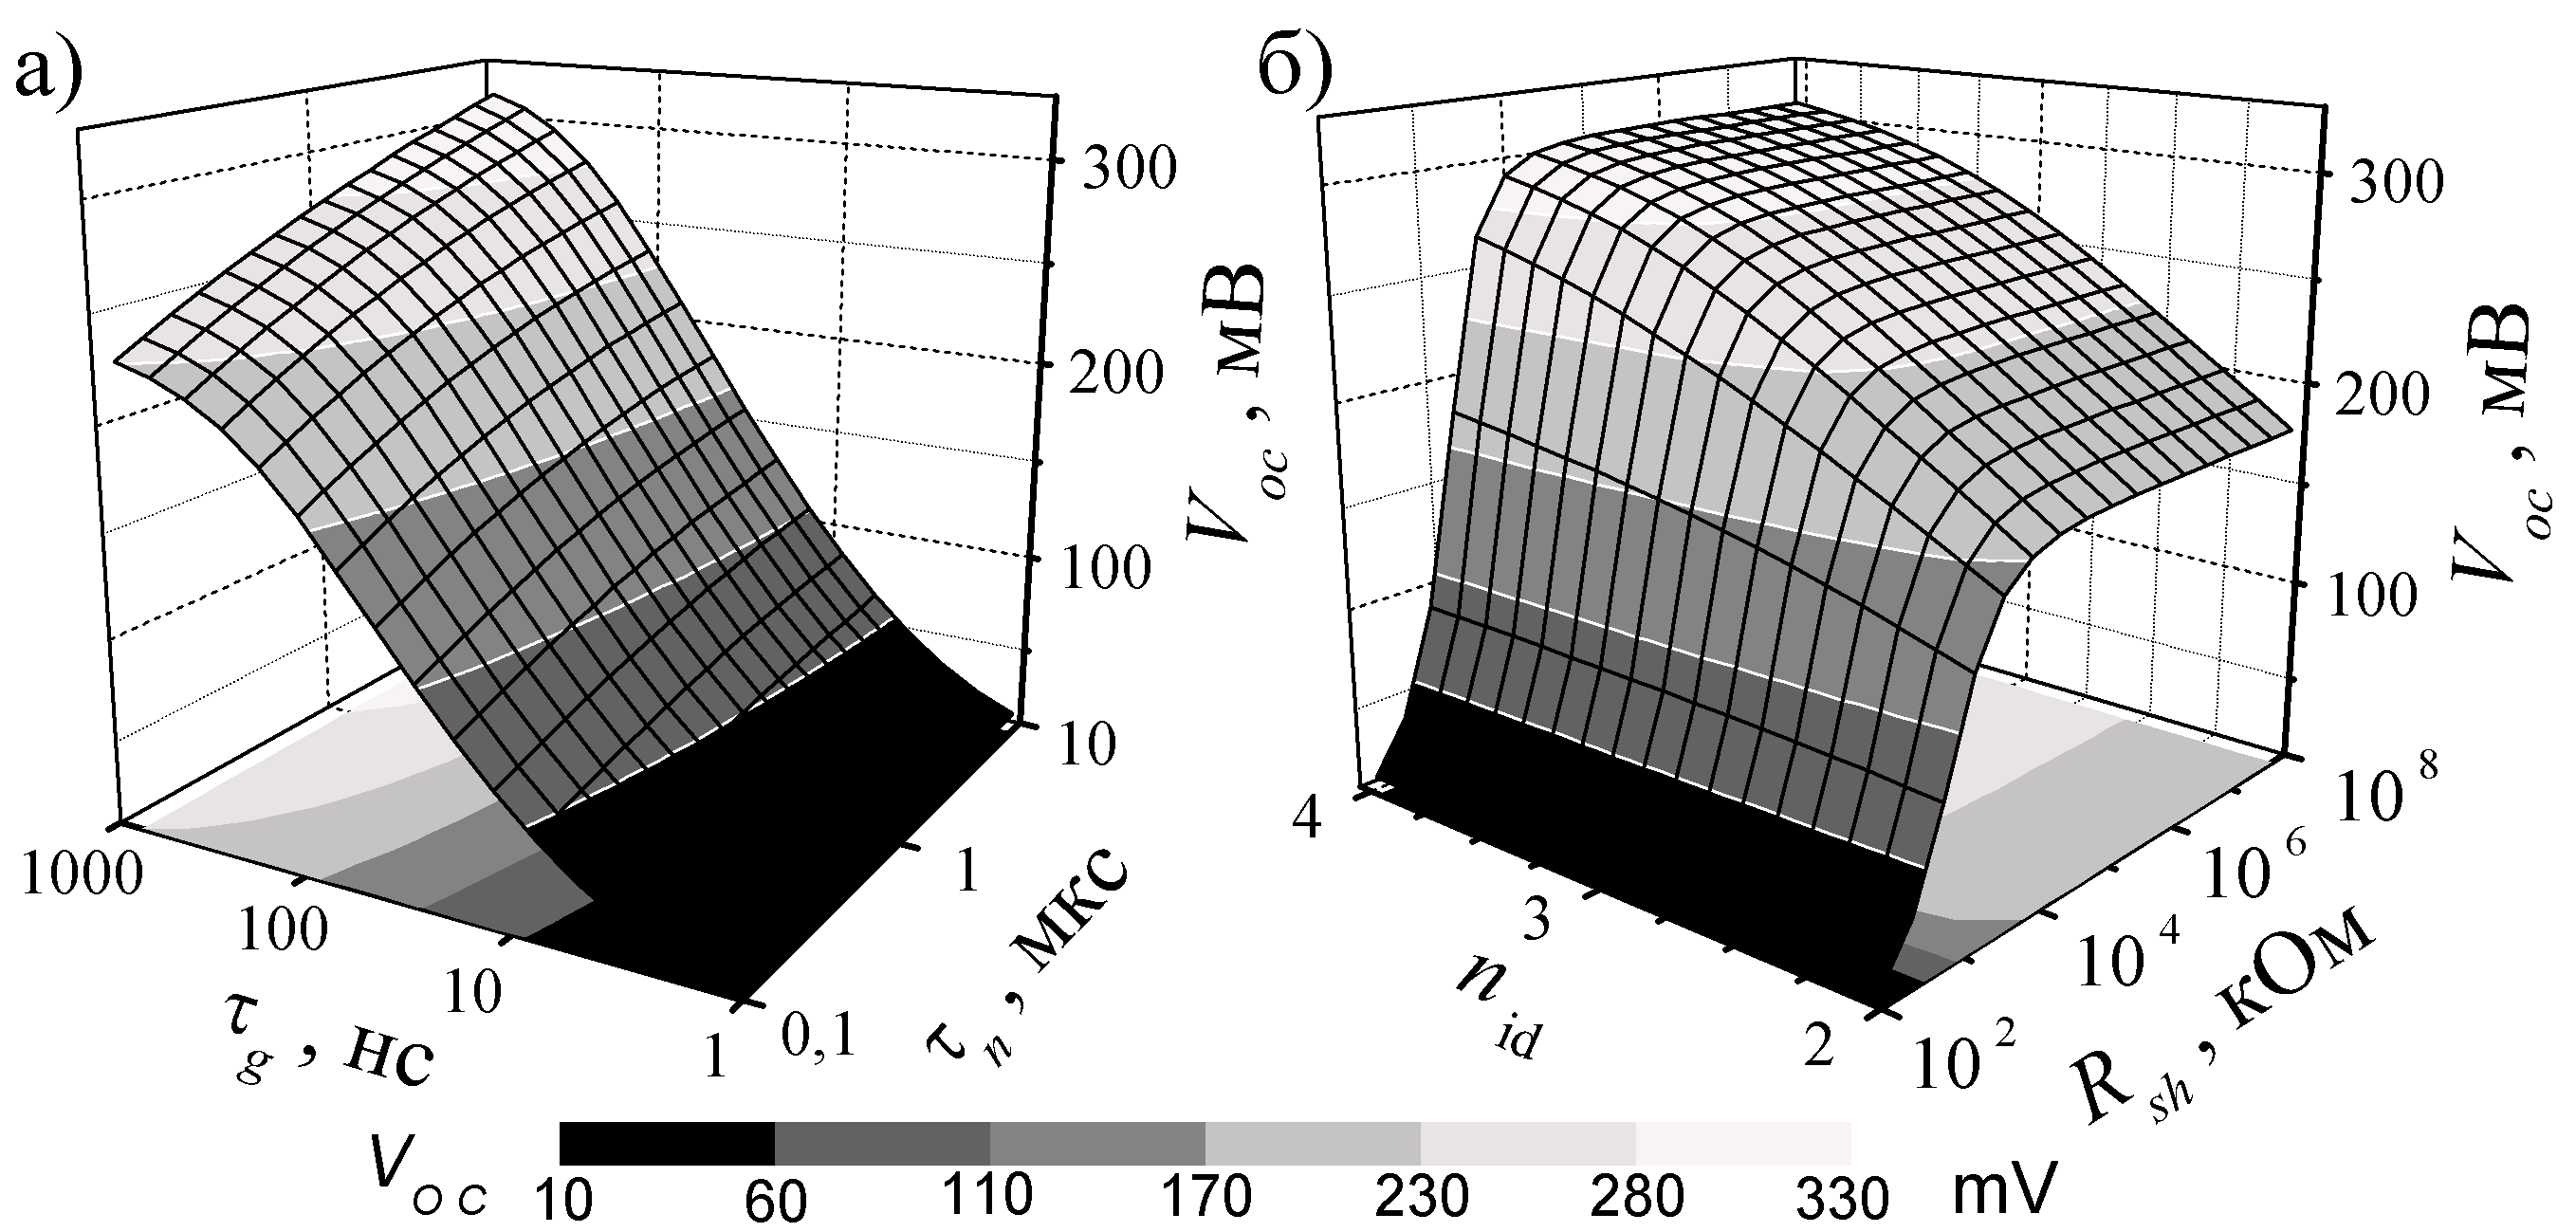
\includegraphics[width=0.95\textwidth]{figVoc}
\caption{\label{figVoc}
Результати моделювання в рамках моделі подвійного діоду залежності напруги холостого ходу КСЕ від часу життя носіїв заряду в ОПЗ та КНО (а) і
фактору неідеальності та шунтуючого опору (б).
При розрахунках вважалося, що $n_\mathrm{id}=2.55$ (a), $R_{sh}=5\times10^3$~Ом (a), $\tau_n=3\times10^{-6}$~с (б), $\tau_g=5\times10^{-8}$~с (б), $T=320$~K,
освітлення монохроматичне ($\lambda=900$~нм) та низькоінтенсивне ($W_{ph}=8$~Вт/м$^2$).
}%
\end{figure}


\begin{figure}
\center
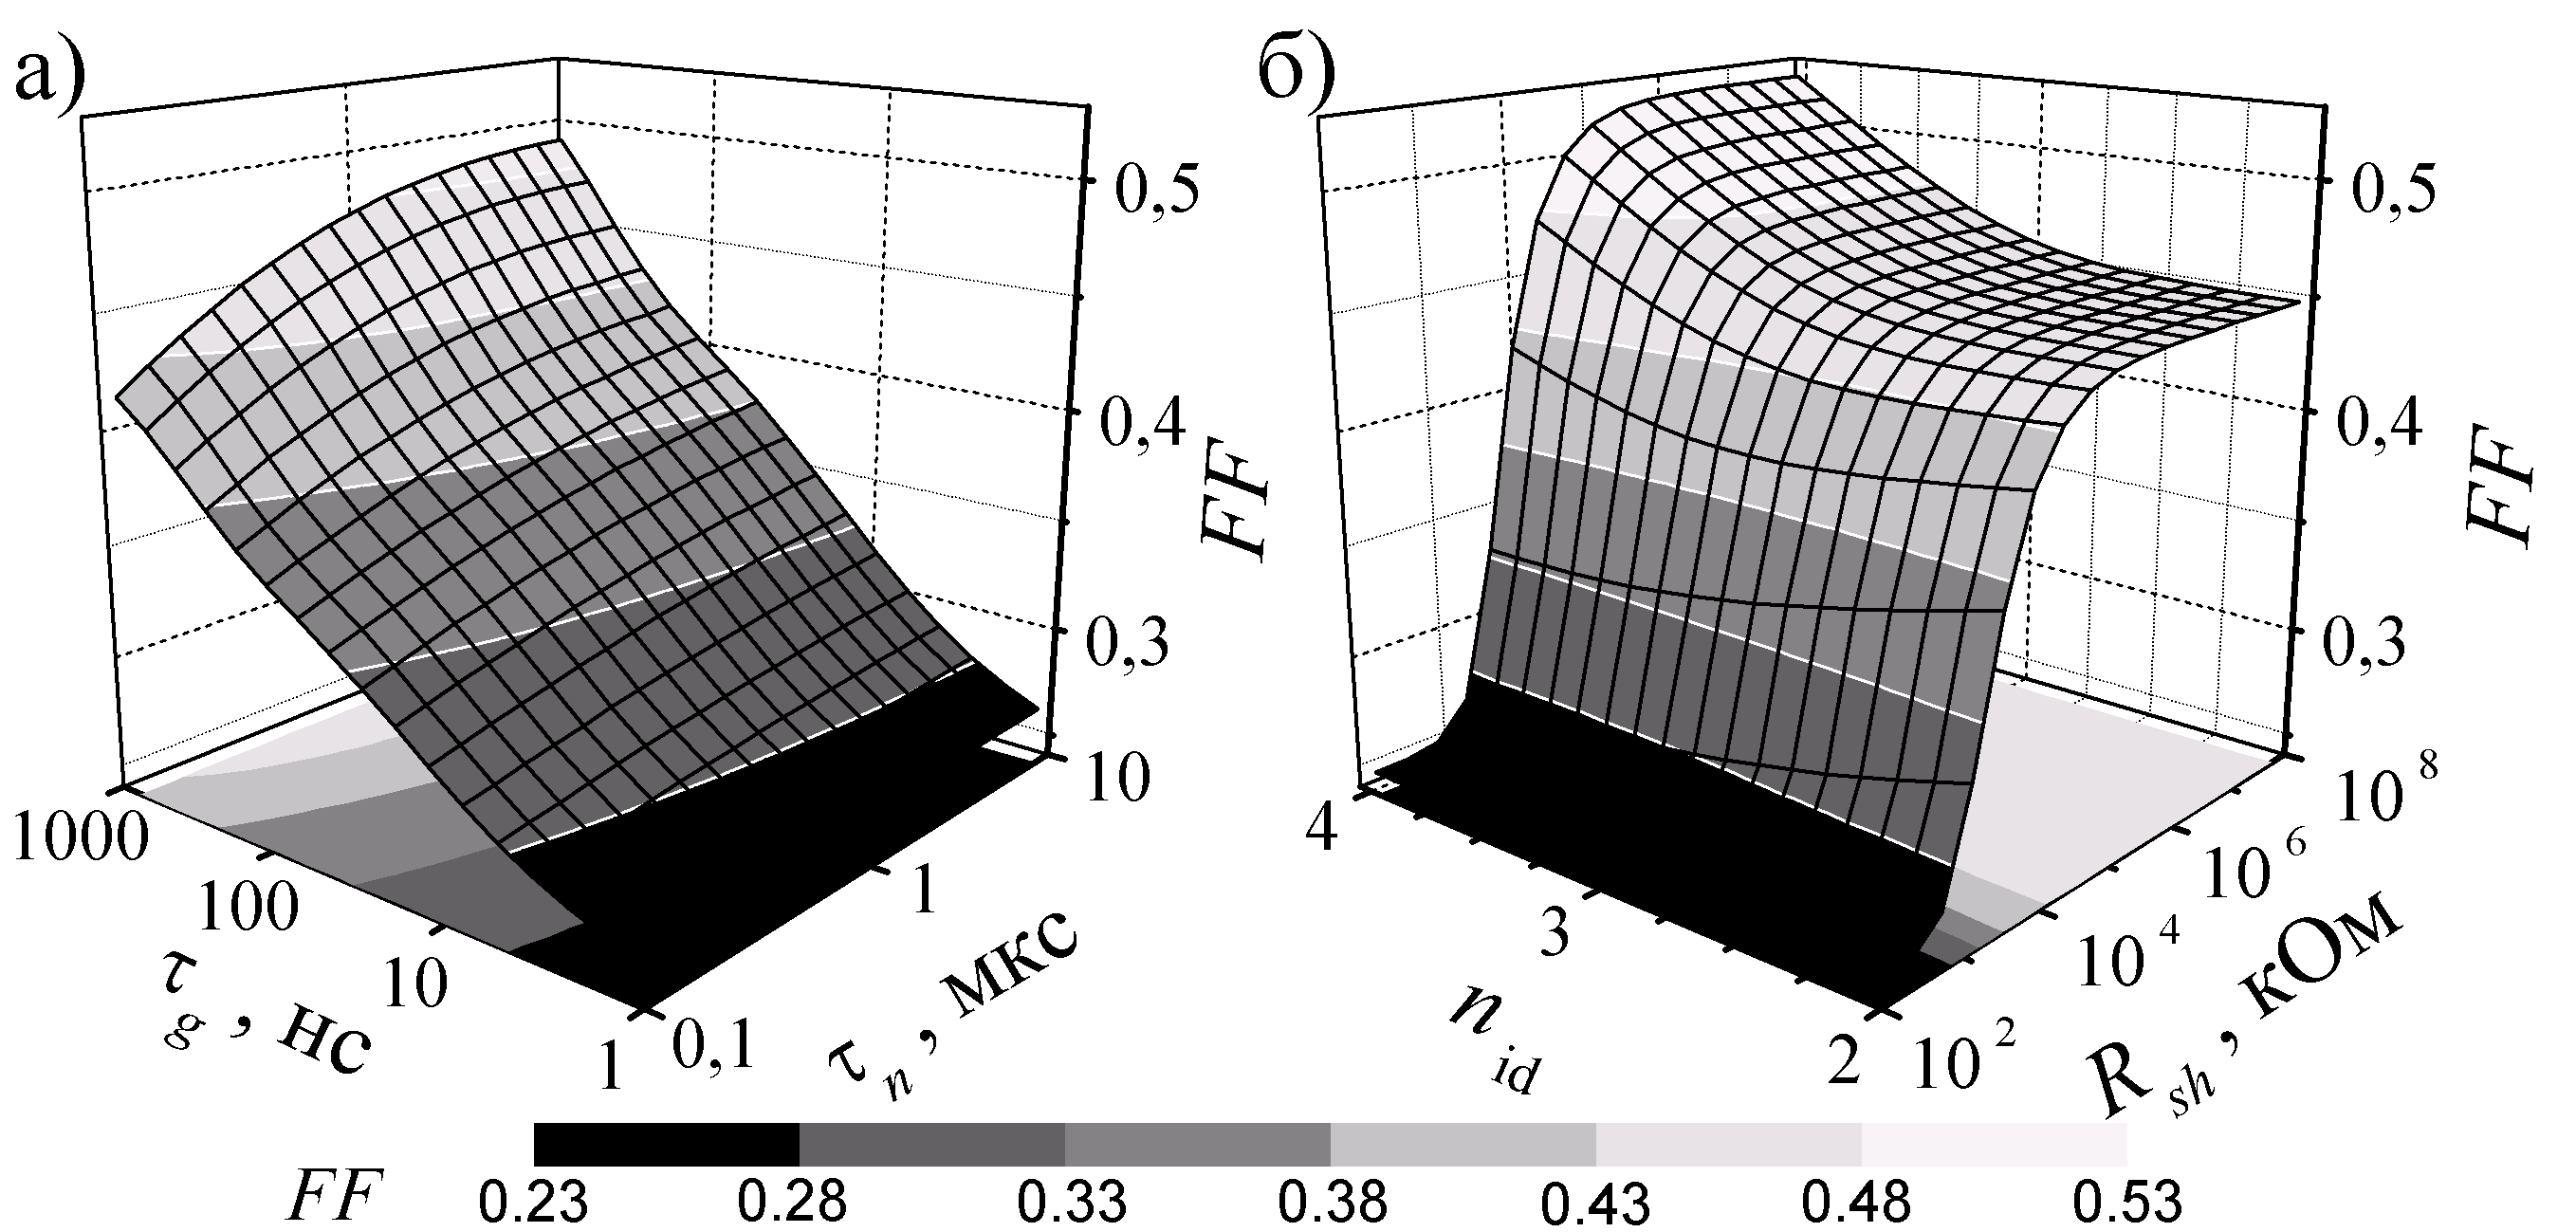
\includegraphics[width=0.95\textwidth]{figFF}
\caption{\label{figFF}
Результати моделювання в рамках моделі подвійного діоду залежності фактору форми СЕ від часу життя носіїв заряду в ОПЗ та КНО (а) і
фактору неідеальності та шунтуючого опору (б).
При розрахунках вважалося, що $n_\mathrm{id}=2.55$ (a), $R_{sh}=5\times10^3$~Ом (a), $\tau_n=3\times10^{-6}$~с (б), $\tau_g=5\times10^{-8}$~с (б), $T=320$~K,
освітлення монохроматичне ($\lambda=900$~нм) та низькоінтенсивне ($W_{ph}=8$~Вт/м$^2$).
}%
\end{figure}

Як видно з Рис.~\ref{figVoc},а та Рис.~\ref{figFF},а, зменшення $\tau_g$ викликає зменшення як $V_{oc}$, так і $F\!F$.
Водночас, для досліджених КСЕ напруга холостого ходу та фактор форми слабко залежать від
часу життя неосновних носіїв в КНО.
Зауважимо, що при розрахунках використовувалися значення $W_{ph}$, яке відповідало експерименту,
тобто розглядалося низько--інтенсивне освітлення.
В цьому випадку величини напруги холостого ходу та напруги, яка відповідає максимуму потужності КСЕ значно нижчі,
ніж при стандартних умовах і тому суттєвий вплив на $V_{oc}$ та $F\!F$ мають саме процеси, які відбуваються
в ОПЗ, тоді як внесок рекомбінації в КНО знижується \cite{Breitenstein2013}.

В свою чергу, Рис.~\ref{figVoc},б та Рис.~\ref{figFF},б показують,
що на величину $V_{oc}$ та $F\!F$ загалом впливає як $n_\mathrm{id}$, так і $R_{sh}$,
проте ступінь цих залежностей суттєво визначається величиною шунтуючого опору.
Наприклад, при $R_{sh}>10^5$~Ом (що відповідає випадку зразка SC17),
а)~$V_{oc}$ зростає з підвищенням величини фактора неідеальності;
б)~$V_{oc}$ та $FF$ практично не залежать від значення $R_{sh}$.
В той же час, при $R_{sh}\leq10^4$~Ом (випадок зразка SCR11),
а)~напруга холостого ходу та фактор форми зменшуються зі зменшенням шунтуючого опору;
б)~лише $F\!F$ слабко залежить від $n_\mathrm{id}$.

Таким чином, розглянута у параграфі \ref{sbQNR} зменшення $\tau_g$ викликає АІ деградацію як напруги
холостого ходу, так і фактора форми.
Цей ефект деградації підсилюється в SC11 внаслідок АІ зменшення $R_{sh}$ та частково компенсується в SC15
через АІ збільшення $n_\mathrm{id}$, що і пояснює відмінність величин $\varepsilon_{Voc}$ та $\varepsilon_{FF}$ в Таблиці~\ref{tabAIEfect}.




\subsection{Вплив інтенсивного освітлення на параметри КСЕ\label{sbDefectType}}
Раніше не було висловлено ніяких припущень, щодо того, які саме дефекти впливають на час життя
носіїв заряду та беруть участь у АДВ.
Даний параграф присвячений розгляду саме цього питання.

Відомо, що основними дефектами, які суттєво зменшують час життя носіїв в кремнії, вирощеному
за методом Чохральського та легованому бором, є
\begin{enumerate}[label=\asbuk*),leftmargin=0em,itemindent=1.5em]
\item  комплекси, що містять бор та кисень (так звані BO дефекти) \cite{LIDRev,LIDRev2};
\item пари залізо--бор \cite{MurphyJAP2011,FeB:Vahanissi,FeB:Schmidt} (або інші залізовмісні пастки, виявлені в $n^+-p$ переходах \cite{TeimurazPSS,TeimurazJAP});
\item кисневмісні преципітати \cite{MurphySC2014,Oxide_Schon,MurphyJAP2011,MurphyJAP2012,Oxide:Chen,Oxide:Porrini}.
\end{enumerate}
Дефекти перших двох типів чутливі до інтенсивного освітлення при кімнатних температурах.
З метою виокремлення впливу окремих дефектів на процеси, що відбуваються у досліджених КСЕ,
після закінчення дослідження впливу УЗ на їх параметри
була застосована наступна експериментальна процедура.

Для інтенсивного освітлення зразків була використана галогенова лампа (інтенсивністю близько 2~Suns).
Освітлення проводилось при температурі близько 305~K,
час одного освітлення вар'ювався в інтервалі від 1 до 8~год.
Після освітлення зразки знаходилися в темряві при кімнатній температурі.
Протягом перших 5~год після закінчення освітлення проводилось вимірювання темнових ВАХ з інтервалом часу $10\div15$~хв.
Метод цих вимірів було визначення кінетики можливих оборотних змін параметрів КСЕ, викликаних освітленням.
Для оцінки величини необоротних змін, також було проведено вимірювання ВАХ та визначення параметрів через 48~год
після освітлення.
Після того, як сумарний час інтенсивного освітлення досягав величини порядку 15~год,
проводився відпал зразків у темряві при температурі 200~$^\circ$C тривалістю 10~хв,
після якого при кімнатній температурі знову проводилось визначення параметрів.
Після цього цикли освітлення--відпал повторювався.

Відомо \cite{LIDRev,LIDRev2}, що інтенсивне освітлення викликає перетворення BO дефектів, що, в свою
чергу, призводить до суттєвого (до 10~\% від вихідного значення при тривалому освітленні) зменшення часу життя неосновних носіїв.
При кімнатній температурі ці зміни є залишковими, ВО дефекти не повертаються до вихідної конфігурації.
Проте десяти--хвилинний відпал при 200~$^\circ$C відновлює рекомбінаційні параметри кристалу, причому
якщо відпал відбувався у темряві, то дефекти повертаються до початкової конфігурації і знову можуть деградувати під
дією світла \cite{BO:Halam2016,LIDRev2,Kim}.

Таким чином, якщо якийсь з параметрів ($\tau_g$, $\tau_n$, $n_{\mathrm{id}}$ чи $R_{sh}$) визначається ВО дефектами,
то внаслідок вибраної експериментальної процедури мають спостерігатися його необоротні зміни після інтенсивного освітлення і відновлення
величини після відпалу.
Якщо припустити, що в досліджених КСЕ конфігурація ВО дефектів одразу відповідала деградованому стану,
то описані в попередньому реченні перетворення мають спостерігатися після першого відпалу.

На Рис.~\ref{figLight} показані стаціонарні значення параметрів зразків після освітлень та відпалів.
Як видно з наведених даних, для різних зразків були використані різноманітні режими.
Проте в будь--якому випадку, освітлення не викликає змін ні $\tau_g$, ні $\tau_n$, ні $n_{\mathrm{id}}$ як до
відпалу так і після.
Отже, можна виключити вплив комплексів, які містять бор та кисень, на рекомбінаційні процеси
як в ОПЗ, так і в базі діоду.

\begin{figure}
\center
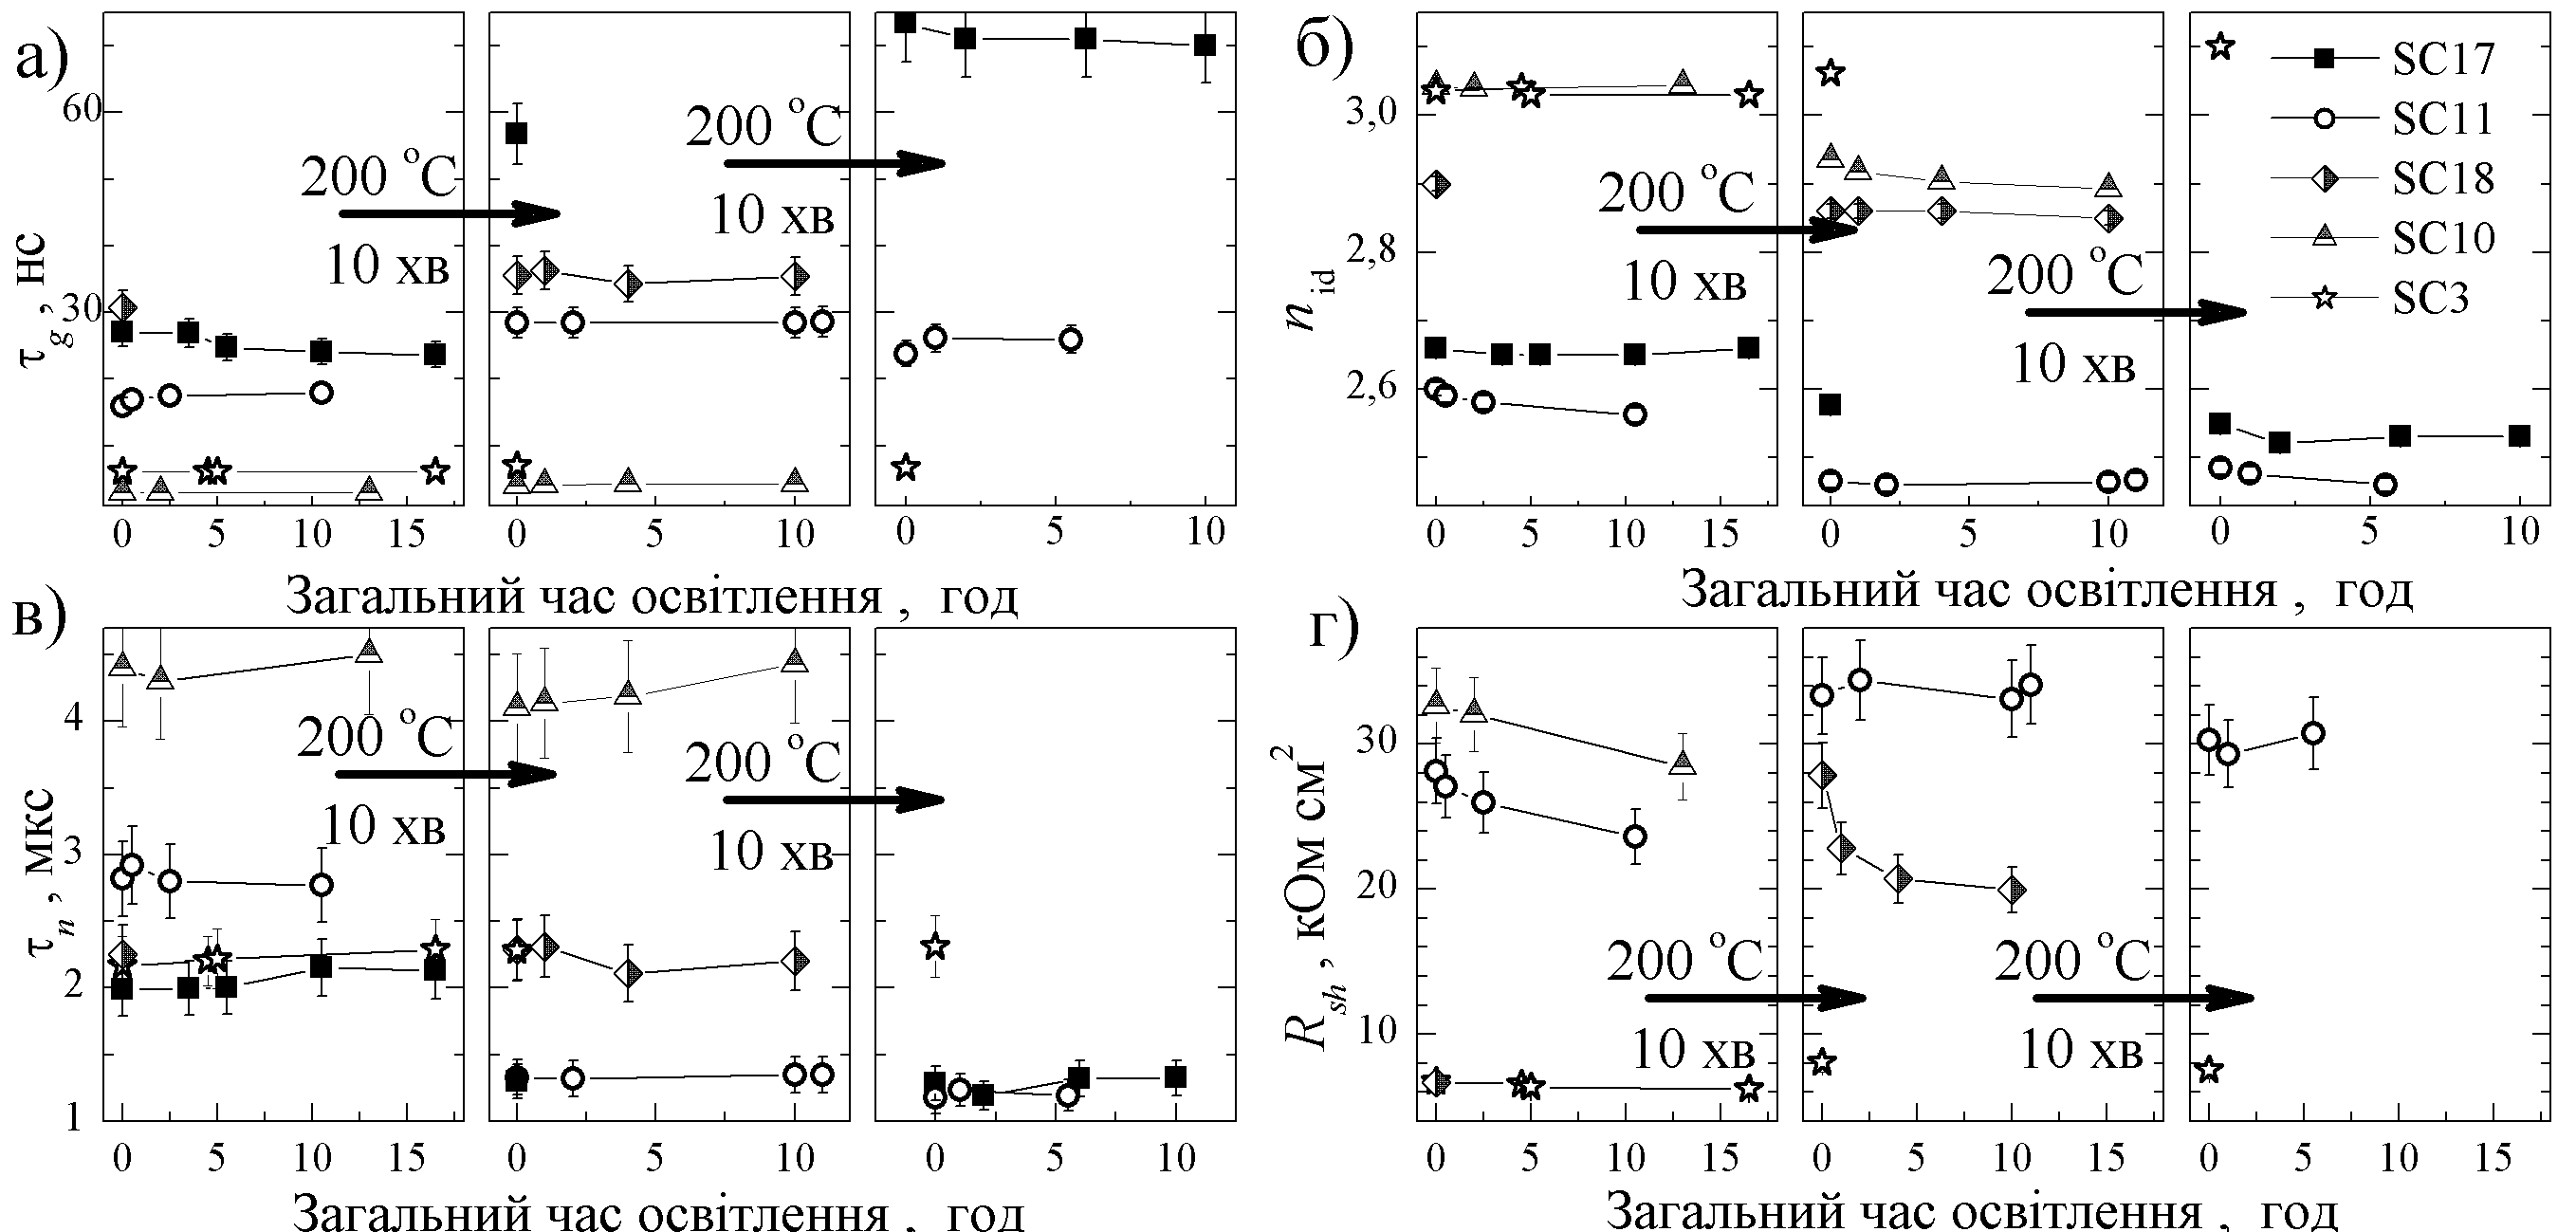
\includegraphics[width=1.0\textwidth]{figLight}
\caption{\label{figLight}
Залежності стаціонарних величин часу життя в ОПЗ (а),  фактору неідеальності (б), часу життя в КНО (в) та шунтуючого опору (г) від
повної тривалості високоінтенсивного освітлення та відпалу.
Лінії наведено лише для зручності.
Для зразка SC10 після першого відпалу значення $R_{sh}>10^{12}$~Ом$\cdot$см$^2$.
}%
\end{figure}


В Si:B переважна кількість домішкових атомів заліза утворює пари з бором.
Водночас пара Fe$_i$B$_s$ достатньо легко дисоціює і звільнені таким чином міжвузольні атоми заліза
викликають зменшення часу життя, яке залежить від рівня легування та концентрації надлишкових носіїв заряду \cite{FeB:Schmidt}.
Після припинення освітлення, в темряві, пари Fe$_i$B$_s$ відновлюються, при цьому
зменшення концентрації Fe$_i$ має описуватися виразом \cite{MurphyJAP2011,Wijaranakula}
\begin{equation}
\label{eqFeB}
N_{Fe}(t)=(N_{Fe,\,0}-N_{Fe,\,eq})\exp\left[-\frac{t}{\tau_{\mathtt{rep}}}\right]+N_{Fe,\,eq}\,,
\end{equation}
де
$N_{Fe,\,0}$ --- концентрація міжвузольних атомів безпосередньо після освітлення,
$N_{Fe,\,eq}$ --- рівноважна концентрація, яка досягається після тривалого перебування кристалу у темряві.
При цьому характерний час утворення пари $\tau_{\mathtt{rep}}$ залежить як від температури, так і від
рівня легування:
\begin{equation}
\label{eqTrep}
\tau_{\mathtt{rep}}=770\cdot p_p^{\,-2/3}\exp\left(\frac{E_{\mathtt{D,\,Fe}}}{kT}\right)\,,
\end{equation}
де
$E_{\mathtt{D,\,Fe}}=0,68$~еВ --- енергія активації дифузії Fe$_i$.


\begin{figure}
\center
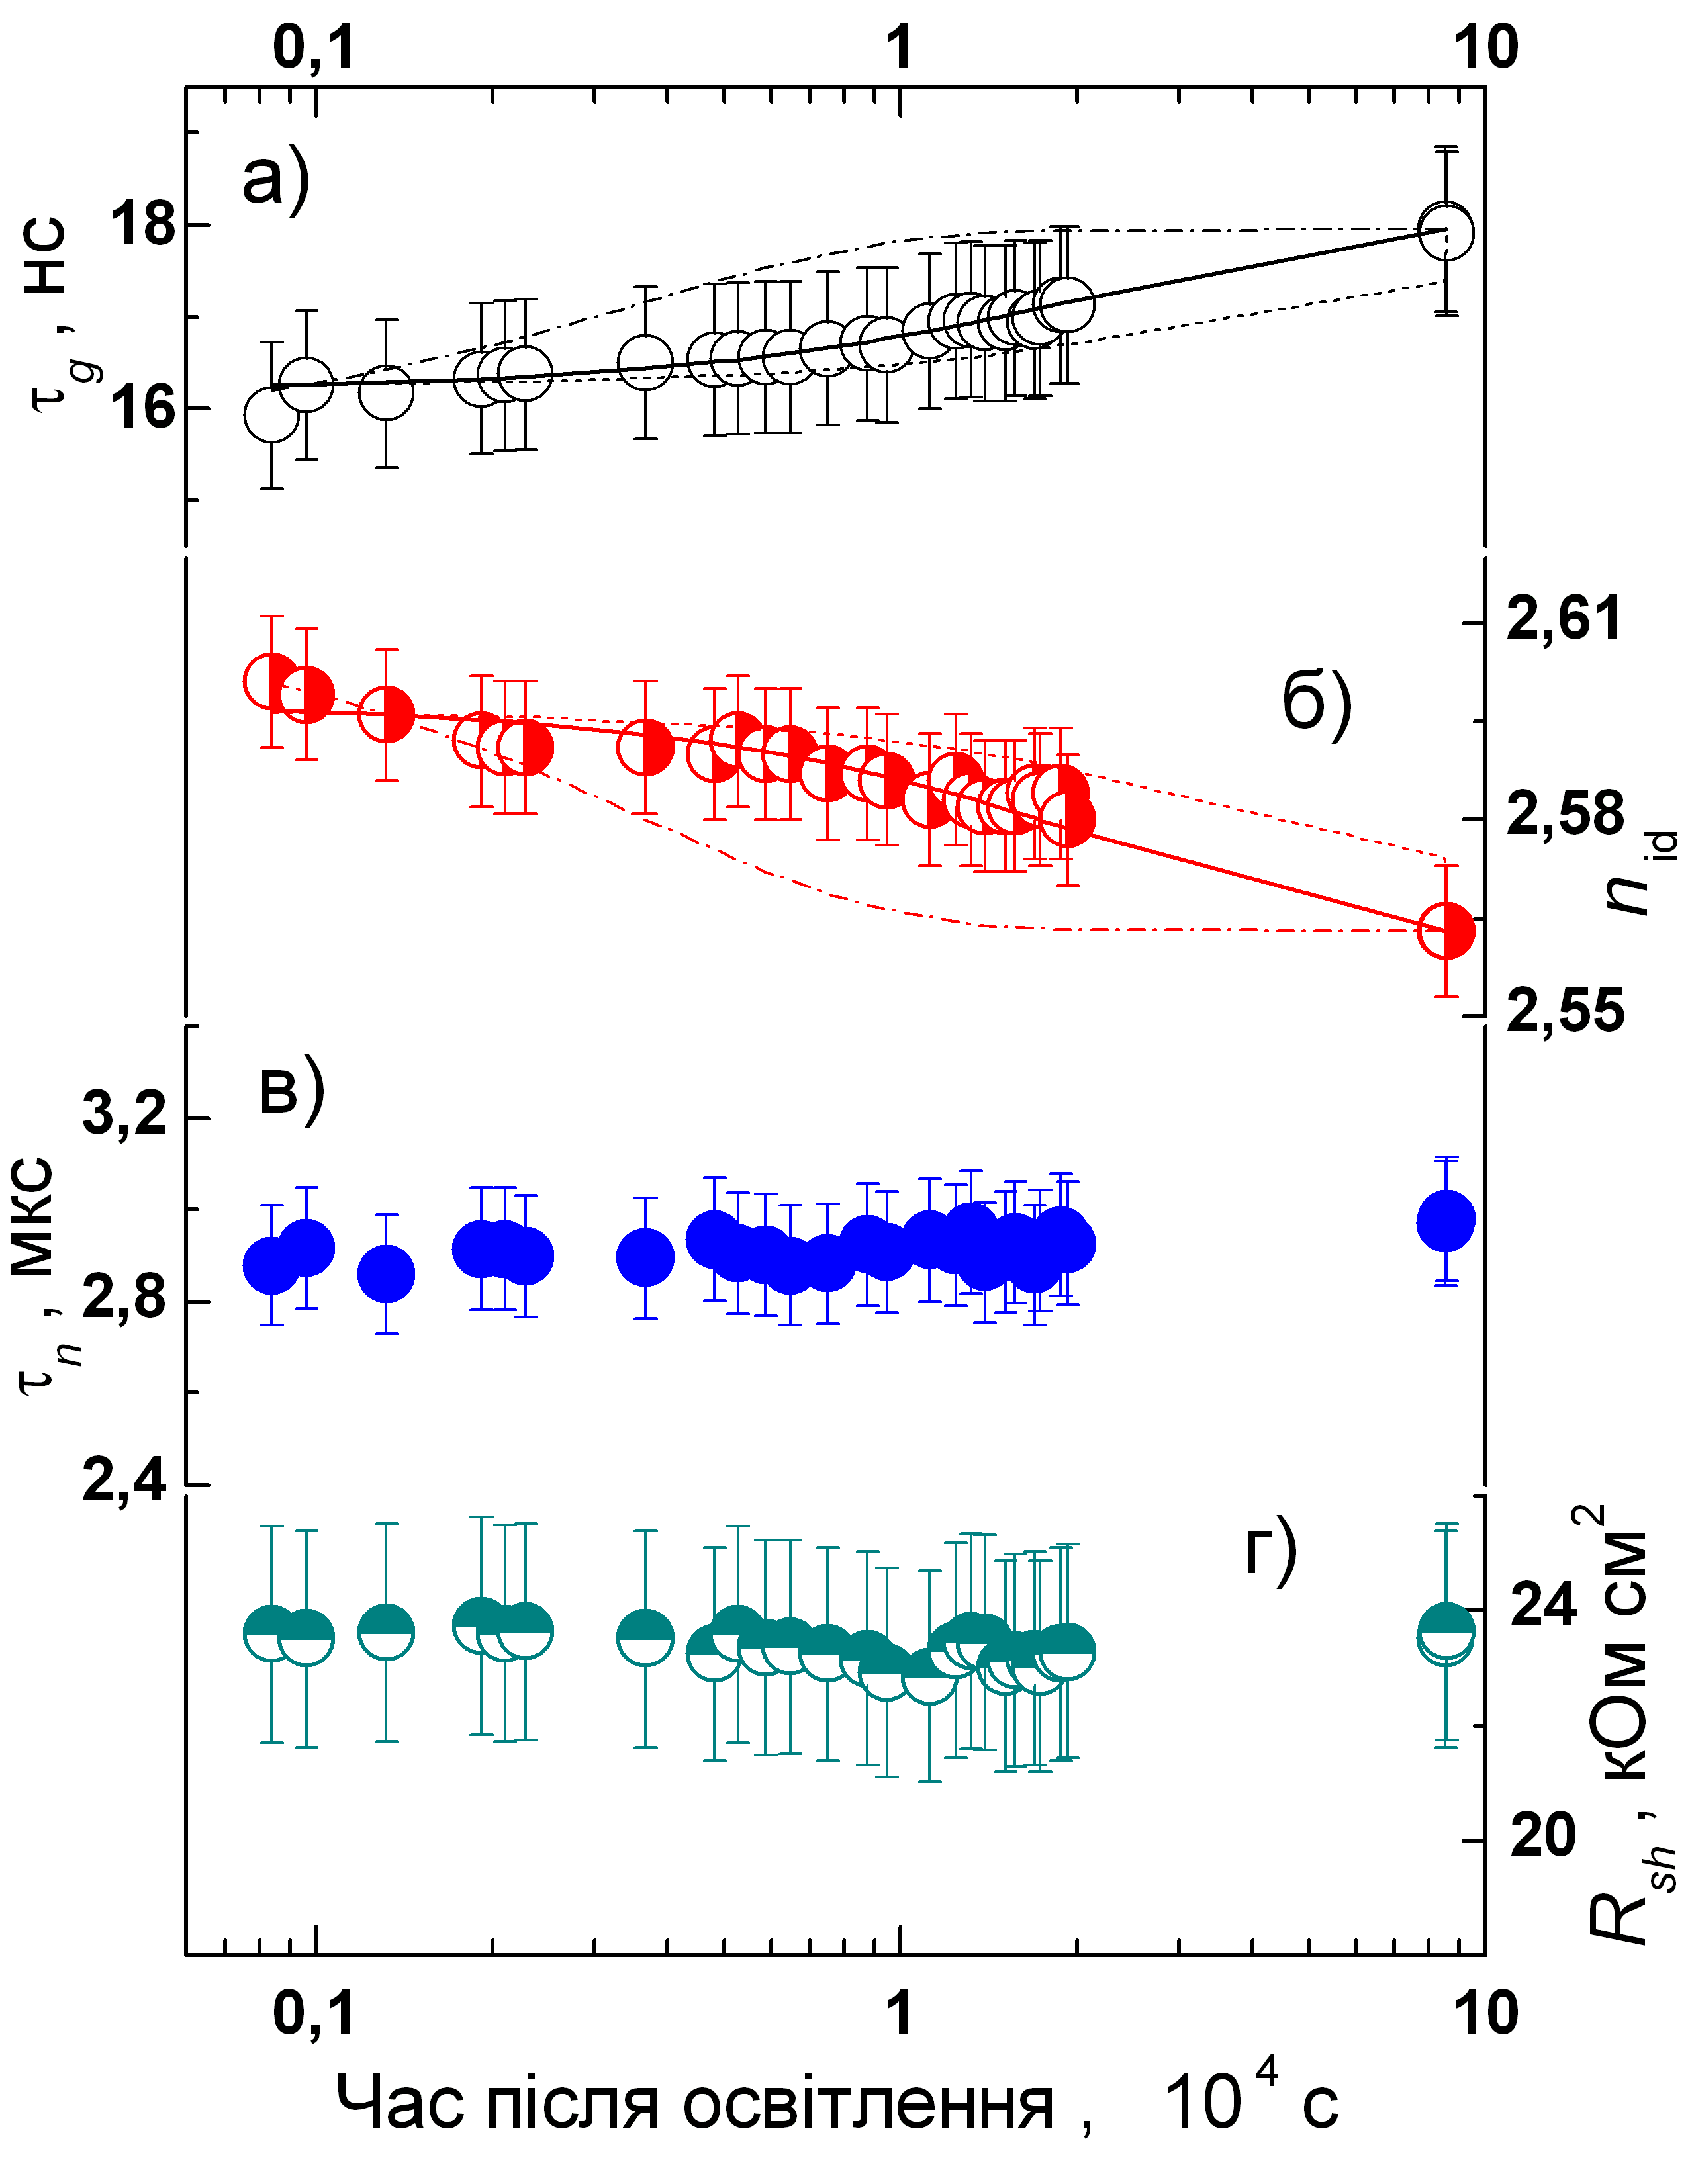
\includegraphics[width=0.65\textwidth]{figAfter}
\caption{\label{figAfter}
Залежність часу життя в ОПЗ (а),  фактору неідеальності (б), часу життя в КНО (в) та шунтуючого опору (г) від часу, що пройшов
після припинення освітлення.
Зразок SC11, $T=295$~K.
Точки --- результати вимірів,
лінії --- апроксимація з використанням формул (\ref{eqFeB}) та (\ref{eqTrep})
і $E_{\mathtt{D,Fe}}=0,63$~еВ (штрих--пунктирна лінія), 0,68~еВ (суцільна лінія) та 0,73~еВ (штрихова лінія).
}%
\end{figure}

Типова релаксаційна залежність зміни параметрів КСЕ після інтенсивного освітлення показана на Рис.~\ref{figAfter}.
Так як $\tau_n$ не змінюється після освітлення (див. Рис.~\ref{figAfter},в), то можна зробити висновок про те, що
пари Fe$_i$B$_s$ суттєво не впливають на час час життя в ОПЗ.

З іншого боку, виявлено збільшення $n_{\mathrm{id}}$ (приблизно на 0.03) та зменшення $\tau_g$ (приблизно на 10~\%) безпосередньо після освітлення
--- див. Рис.~\ref{figAfter},а та Рис.~\ref{figAfter},б.
В темряві ці зміни поступово зникають.
Було зроблено припущення, що еволюція $\tau_g$ та $n_{\mathrm{id}}$ може бути описана виразом, подібним до (\ref{eqFeB}).
При використанні величини $\tau_{\mathtt{rep}}=\left[1,3\cdot10^{-3}(1,4\times10^{15})^{\,2/3}\exp\left(-\frac{0,68}{295k}\right)\right]^{-1}=2,53\cdot10^4$~с,
яка очікується для відомого значення $E_{\mathtt{D,Fe}}=0,63$~еВ, апроксимуюча крива достатньо добре збігається з експериментальними даними
(суцільні лінії на Рис.~\ref{figAfter},a та б).
В той же час застосування іншої величина для $E_{\mathtt{D,Fe}}$ викликає суттєві відмінності між розрахованими та виміряними величинами
(штриховані лінії на цьому ж рисунку).
Отримані результати свідчать на користь того, що пара залізо--бор впливає
на рекомбінацію в ОПЗ.
Заряд пари в основному стані дорівнює <<+1>>, а отже у CDLR процесах має відігравати роль донора.
%, а її акцепторний рівень $E_c-0.26$~еВ \cite{MurphyJAP2011} приймає участь у CDLR процесах.
%При цьому
З одного боку, пара Fe$_i$B$_s$ є непоганим кандидатом на роль ААД:
бор є домішкою заміщення з іонним радіусом, який менший ніж для Si ($\Delta\Omega_d (\mbox{B}_s)<0$),
тоді як для міжвузольного заліза $\Delta\Omega_d (\mbox{Fe}_i)>0$.
Більше того,  в літературі \cite{Ostapenko1995,OlikhFTT} представлені результати впливу УЗН на цей дефект.
Проте з іншого боку, ППЗ електронів та дірок для Fe$_i$ та Fe$_i$B$_s$ відрізняються досить суттєво, в 1,7 та 0,04 рази, відповідно \cite{MurphyJAP2011}.
А так як, $\tau_g$ змінюється під дією світла незначним чином (приблизно на 10~\%, що навіть менше ніж в умовах УЗН), то це свідчить про
неосновну роль пари як у рекомбінаційних процесах в ОПЗ, так і в АДВ у цій області.


Таким чином, можна зробити висновок, що рекомбінація як в ОПЗ, так і в КНО відбувається, переважно,
завдяки кисневмісним преципітатам (КП).
За своєю будовою  це скупчення SiO$x$ ($1\leq x\leq2$), які утворюються всередині кристалу кремнію при підвищених температурах.
Розмір цих утворень коливається від декількох десятків до декількох сотень ангстрем залежно від режиму обробки.
При їх утворенні у загалом бездислокаційному Cz--Si виникають лінійні дефекти та дефекти пакування \cite{SiO:Hwang,SiO:Vanhell}.
Наявність КП суттєво впливає на час життя носіїв як в ОПЗ, так і в КНО.
наприклад, у кристалах з високою концентрацією преципітатів довжина дифузії неосновних носіїв може зменшуватись до декількох мікрон \cite{SiO:Hwang}.
Водночас КП виконують роль гетерів для домішкових атомів металів, які неминуче потрапляють у кристал під час виробництва
інтегральних схем і відіграють згубну роль для їх властивостей \cite{APR:Oxigen,MSER74}.
Цей процес гетерування є дуже важливим з точки зору збільшення відсотку виходу придатної мікроелектронної продукції.
Проте за наявності надмірної кількості КП та супроводжуючих їх появу дислокації
спостерігається зменшення механічної міцності Cz--Si \cite{MSER74}.


В досліджуваних зразках утворення певної кількості цих дефектів, і, відповідно, зменшення $\tau _n$ могло відбутися під час відпалу,
який застосовувався для переведення імплантованих іонів фосфору у електрично--активний стан.
Подібні процеси відомі з літератури.
Наприклад, в роботі \cite{SiO:Miyagi} показано, що відпал при температурі 750--850$^\circ$C
може викликати збільшення концентрації КП та зменшення часу життя.

З точки зору моделі CDLR це також цілком придатні об'єкти.
Дійсно, згідно з результатами, представленими в \cite{MurphySC2014,MurphyJAP2012},
рекомбінацію на SiO$x$ не можна пояснити використовуючи наближення одного дефекту, якому відповідає два рівні у забороненій зоні,
необхідно розглядати щонайменше два незалежних дефекти.
Цим дефектам відповідають рівні $E_v+0.22$~еВ та $E_c-0.08$~еВ, причому для них $\sigma_n/\sigma_p=157$ та $\sigma_p/\sigma_n=1200$ \cite{MurphyJAP2012}.
Тобто, ці дефекти цілком можуть виконувати роль донора та акцептора в моделі CDLR.
Як вже згадувалось, очікується, що процеси CDLR відбуваються переважно в околі лінійних дефектів \cite{CDLR:JAP,CDLR:SSP}.
Водночас, в літературі \cite{MurphySC2014,MurphyJAP2011,MurphyJAP2012} показано, що дислокації та дефекти пакування,
які оточують КП, можуть змінювати ППЗ та збільшувати концентрації двох вищеназваних дефектів,
проте не викликають появу  нових рівнів у забороненій зоні.

В літературі \cite{MurphyJAP2011} також показано, що ефективний коефіцієнт захоплення носіїв кисневмісними
преципітатами збільшується в декілька разів за умов перебування дефекту в полі механічних напруг.
В нашому випадку додатковим джерелом подібних напруг, поряд
з оточуючими КП дислокаціями та дефектами пакування, є УЗ і тому зменшення
часу життя носіїв може бути викликано і цією причиною також.

Скупчення SiO$x$, як правило, нерівномірно розподілені по площі пластини  Cz--Si \cite{Oxide_Schon} або сонячних елементів \cite{Oxide:Chen}.
Це може бути причиною зміни параметрів від зразка до зразка.
Нарешті,  стан КП залежить від обробки кристалу при підвищеній температурі.
В досліджених структурах відпал, на відміну від освітлення, викликає певні зміни параметрів (див. Рис.\ref{figLight}).
Виявлені зростання $\tau_g$ і $R_{sh}$ та спад $\tau_n$ і $n_\mathrm{id}$, на нашу думку, пов'язані саме з видозміною КП.

З іншого боку, дефекти різного типу зустрічаються в кремнієвих структурах одночасно.
Наприклад, у роботі \cite{BO:Fe} показано, що значна частина експериментальних особливостей зміни часу життя
внаслідок утворення ВО--дефектів може бути пояснена наявністю (та світло--індукованим розпадом) пар  Fe$_i$B$_s$.
А саме, визначальними для величини $\tau_n$ є комплекси, що містять бор та кисень, проте
наявність домішкового заліза впливає на процеси визначення параметрів кристалу.
Подібна супутникова роль пар Fe$_i$B$_s$ спостерігається і в нашому випадку.

Таким чином, на підставі зазначених вище даних, можна зробити висновок,
що дефектами, які приймають участь як у рекомбінаційних процесах, так і у акусто--дефектній взаємодії є, переважно,
кисневмісні преципітати.
Крім того, певний внесок у ці процеси пов'язаний з парами Fe$_i$B$_s$.

\section{Зміна активності рекомбінаційних центрів у кремнієвих $p$--$n$ структурах за умов ультразвукового навантаження\label{sBulyrMethod}}

\subsection{Метод визначення енергетичного положення рівнів в ОПЗ}

Методи нерівноважної модифікації дефектно--домішкової підсистеми з метою отримання нових властивостей напівпровідникових
кристалів, структур чи приладів, тобто методи так званої <<інженерії дефектів>> викликають все більшу зацікавленість дослідників \cite{Smirnov}.
Це зумовлено перспективами  створення за допомогою подібних методів елементної бази твердотільної
електроніки нового покоління за рахунок контрольованого формування та видозміни активних центрів або нанокластерів.
Безумовні, лідерами цієї галузі є радіаційні методи --- див., наприклад, \cite{Kozlovs,DefImplan}.
Проте цікаві результати отримані і при дослідженнях альтернативних способів впливу на дефектну підсистему напівпровідників,
зокрема при використанні з цією метою АХ.
Наприклад, УЗО стимулює перегрупування дефектів \cite{ZobovFTP2008}, розпад \cite{PodolHivr} та утворення \cite{YOlikh2006TPLr} різноманітних комплексів,
формування наночастинок \cite{Roman:2006JAP} в об'ємі напівпровідника,
зміну концентрації дефектних центрів на границі розділу окис--напівпровідник \cite{Parchinskii2006r}.
Однією з переваг використання УЗ є можливість перебудовувати дефекти оборотним чином, що відкриває
перспективи створення функціональних електронних пристроїв з динамічним керуванням характеристиками.

В цьому параграфі представлені результати експериментального дослідження впливу УЗН на енергетичне положення в забороненій зоні та
рекомбінаційну активність електронних станів, пов'язаних з дефектами в кремнієвих $p$--$n$ структурах.
Для досліджень використовувалися зразки, вирізані як з центральної частини платини, так і з області поблизу її краю (SC11A та SC3, див. Рис.~\ref{SSC}).
Подібний вибір викликаний тим, що розподіл дефектів по площі напівпровідникової пластини неоднорідний і, відповідно, можна було очікувати
певну відмінність у впливі УЗ.

Параметри ГР визначалися згідно з методикою, яка запропонована в \cite{Bulyar}.
Вона базується на вивченні диференційного показника нахилу ВАХ $\zeta$:
\begin{equation}\label{BetaVAX}
  \zeta=\frac{qI}{kT}\left(\frac{\partial I}{\partial V}\right)^{-1}\,.
\end{equation}
Кількість максимумів на залежності $\partial \zeta/ \partial V = f (V)$ має відповідати кількості різних типів глибоких
рівнів у забороненій зоні напівпровідника,
які ефективно приймають участь у рекомбінації носіїв заряду.
При цьому енергія термічної активації $i$--го ГР $E_c-E_{t,i}$ визначається абсцисою
відповідного максимуму $V_{0,i}$:
\begin{equation}\label{eqBulEt}
  E_c-E_{t,i}\approx \frac{E_g-q V_{0,i}}{2}\,.
\end{equation}
Формула~(\ref{eqBulEt}) справедлива з точністю до систематичної похибки $\delta_{Et}$,
що залежить від матеріалу і властивостей ГР.
Так, для випадку рівнів, розташованих у верхній половині забороненої зони вона визначається виразом
$\delta_{Et}=\frac{kT}{2}\ln\left(\frac{c_n N_c}{c_p N_V}\right)$
(де $c_n$ та $c_p$ --- усереднені по всім станам коефіцієнти захоплення електрону та дірки цим центром).
Проведені оцінки показали, що для кремнію при $c_n/c_p=10$ та кімнатній температурі $\delta_{Et}\approx0,02$~еВ.
Амплітуда кожного з максимумів визначається внеском у рекомбінацію того чи іншого центру \cite{Bulyar}.

Була використана наступна процедура.
Виміряна ВАХ коректувалася з врахуванням величини шунтуючого опору і на її основі будувалася залежність $\partial \zeta/ \partial V = f (V)$.
Після цього проводилася апроксимація отриманої залежності сумою гаусових кривих,
кількість яких визначалась кількістю максимумів.
Використовуючи знайдені таким чином $V_{0,i}$ за допомогою Формули~(\ref{eqBulEt}) були розраховані
значення $E_c-E_{t,i}$ для кожного ГР.
При цьому також проводилась оцінка відносного внеску $\eta_i$ кожного з максимумів у загальну площу
\begin{equation}\label{eqBulEta}
  \eta_i=\frac{S_i}{S_\Sigma}\,,
\end{equation}
де
$S_i$ --- площа під гаусіаною, яка описує $i$--ий максимум,
$S_\Sigma$ --- загальна площа під всією апроксимуючою кривою.
Надалі величина $\eta_i$ розглядалась як показних питомого внеску у загальну рекомбінацію
кожного з ГР.

\subsection{Виявлені рівні та їх можлива ідентифікація}

На Рис.~\ref{figBul1},а наведена виявлена залежність $\partial \zeta/ \partial V $ для зразка SC11A.
На ній спостерігається три максимуми, що, згідно з \cite{Bulyar}, свідчить про наявність
трьох типів рівнів, що визначають генераційно--рекомбінаційні процеси під час проходження струму.
Ці рівні надалі позначені Е1, Е2 та Е3.
Абсциси максимумів дорівнюють, відповідно, 0,14, 0,21 та 0,28~В.
Розрахунок за формулою~(\ref{eqBulEt}) показав,
що  $E_c-E_{t,i}$ для рівнів  Е1, Е2 та Е3 складає величини $(0,48\pm0,01)$, $(0,44\pm0,01)$ та $0,40\pm0,01)$~еВ, відповідно --- див. Таблицю~\ref{tabBulEtUSL}.
З наведеної на Рис.~\ref{figBul1},а видно, що за відсутності УЗН максимальний внесок у рекомбінацію робить найбільш глибокий рівень.


\begin{figure}
\center
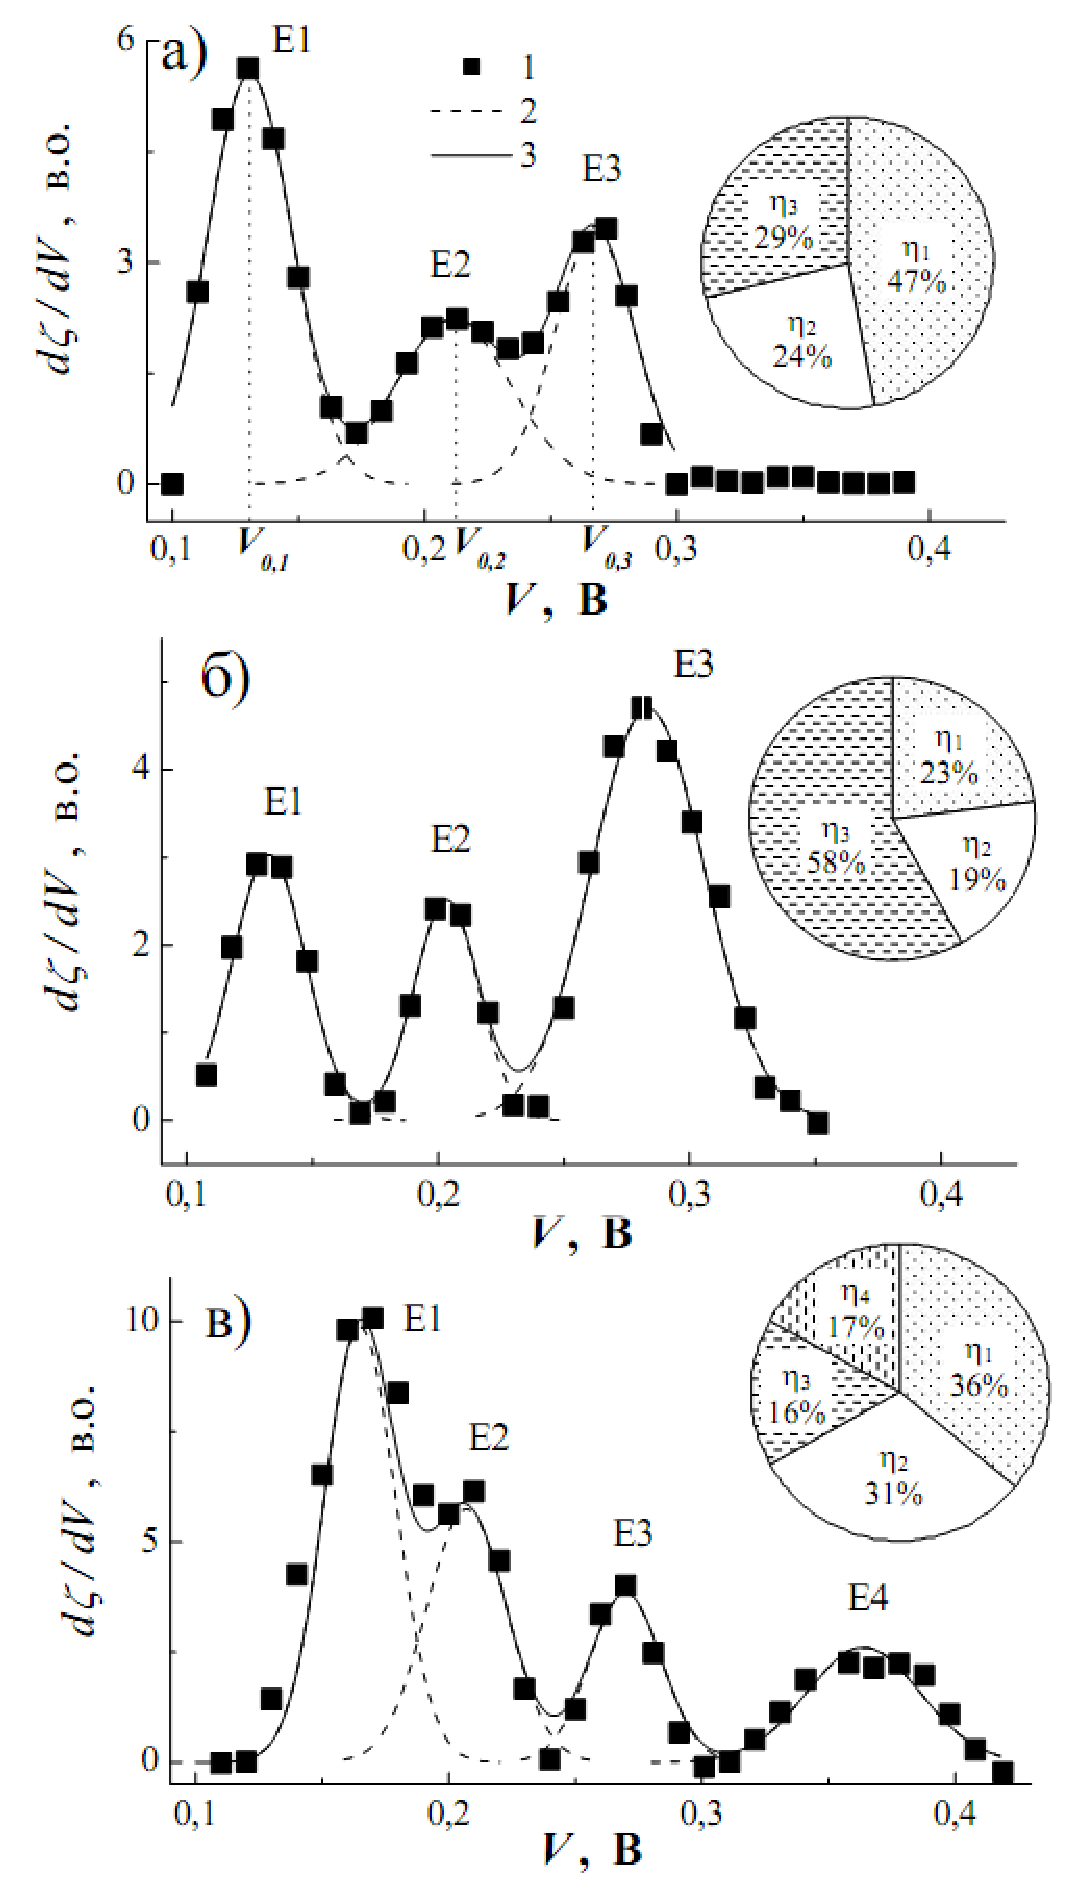
\includegraphics[width=0.6\textwidth]{figBul1}
\caption{\label{figBul1}
Польова залежність похідної диференційного показника нахилу ВАХ за відсутності УЗН (а)
та за його наявності (U--L26t, $W_\mathtt{US}=0,1$~Вт/см$^2$ та U--L4t,  $W_\mathtt{US}=0,25$~Вт/см$^2$ для б та в, відповідно).
1 --- точки, отримані після диференціювання експериментальних ВАХ,
2 --- гаусіани, якими апроксимувалися максимуми,
3 --- сума всіх гаусіан.
Зразок SC11A.
Справа біля кривих наведено діаграми питомих внесків $\eta_i$ кожного з максимумів у загальну криву.
}%
\end{figure}


\begin{table}
\caption{\label{tabBulEtUSL}Порівняння отриманих значень енергій активації глибоких рівнів та літературних даних.
}
\center
\begin{tabular}{|c|c|c|c|c|c|c|c|}
\hline
\multicolumn{5}{|c|}{Отримані результати}&\multicolumn{3}{c|}{Літературні дані}\\ \hline
&\multicolumn{2}{c|}{SC11A}&\multicolumn{2}{c|}{SC3}&&&\\ \cline{2-5}
Рівень&без УЗ&УЗН&без УЗ&УЗН&$E_c-E_t$,&Тип&Джерело\\ \cline{2-5}
&\multicolumn{4}{c|}{$(E_c-E_t)$, $\pm0,01$~еВ}&еВ&дефекту&\\
\hhline{========}
Е1&0,48&0,47&0,48&0,48&0,475&COV$_2$&\cite{Lugakov}\\\cline{6-8}
&&&&&0,50--0,52&дисл.&\cite{Edis:Ogawa,Edis:Omling,Kittler2003}\\ \hline
Е11&---&---&0,46&0,46&0,46&V$_3$&\cite{V3:PRB2012,V3:Markevich}\\ \cline{6-8}
&&&&&0,46&V$_2$O&\cite{V2:JAP2014}\\ \cline{6-8}
&&&&&0,46&V$_3$O&\cite{V3:Markevich}\\ \hline
Е2&0,44&0,425&0,43&0,42&0,42--0,46&VP$_s$&\cite{VI:Luc,Kuchinskii,Karazh,Ecentre:2005}\\ \cline{6-8}
&&&&&0,43&дисл.&\cite{SiO:Vanhell}\\ \cline{6-8}
&&&&&0,43--0,44&V$_2$&\cite{V2:JAP2014,V2:PRB2002}\\ \cline{6-8}
&&&&&0,43&Fe$_i$B$_s$$^\mathtt{orth}$&\cite{FeB:PhysRevB49,Istratov1999}\\ \cline{6-8}
&&&&&0,45&Fe$_i$O$_i$&\cite{FeO}\\ \cline{6-8}
&&&&&0,43--0,44&Si$_i$&\cite{VI:Luc,Si:Sii}\\ \hline
Е3&0,40&0,40&0,40&0,39&0,41&BO$_\mathtt{SRC}$&\cite{LIDRev,LIDRev2,Rein,LID:SchmidtJMR}\\ \cline{6-8}
&&&&&0,41--0,43&SiO$_x$&\cite{SiO:Mchedlidze,SiO:Vanhell,SiO:Chan}\\ \cline{6-8}
&&&&&0,39&V&\cite{MSER55}\\ \hline
Е4&---&0,37&0,37&0,355&0,36--0,38&BO$_\mathtt{FRC}$& \cite{LIDRev2,BOSingle:SEMSS2017}\\ \cline{6-8}
&&&&&0,37&B$_i$&\cite{Lugakov}\\ \cline{6-8}
&&&&&0,34--0,36&V$_3$&\cite{V3:PRB2012,V3:Markevich}\\ \cline{6-8}
&&&&&0,34&V$_3$O&\cite{V3:Markevich}\\ \cline{6-8}
&&&&&0,37--0,39&дисл.&\cite{PhysRevB56:10208,kveder2008,SiO:Hwang,disl10:Isakova,Kittler2003}\\ \cline{6-8}
&&&&&0,36; 0,39&Si$_i$&\cite{MSER55,Si:Sii}\\ \hline
\end{tabular}
\end{table}



Під час УЗН картина максимумів змінюється --- див. Рис.~\ref{figBul1},б та Рис.~\ref{figBul1},в.
А саме, змінюються співвідношення площ під максимумами (внески в рекомбінацію різних ГР),
відбувається незначний зсув положення максимумів (зміна енергії активації ГР),
змінюється кількість максимумів (проявляються новий ГР).
Зокрема, при U--L4t та U--L8t з'являється сигнал ще від одного ГР,
позначеного Е4, для якого $E_c-E_{t,i}=(0,37\pm0,01)$~еВ.
Більш детально АІ зміни розглянуті в параграфі~\ref{sbBul3}.


Результати, отримані для SC3, наведено на Рис.~\ref{figBul2} та в Таблиці~\ref{tabBulEtUSL}.
Видно, що в цьому випадку картина більш складна, ніж для SC11A:
навіть за відсутності УЗН присутній максимум Е4 та, крім того,
спостерігається ще один максимум, позначений Е11, який пов'язаний з рівнем $E_c-E_{t,i}=(0,46\pm0,01)$~еВ.
Характер АІ змін для SC3, загалом, збігається з виявленими в SC11A ефектами.




\begin{figure}
\center
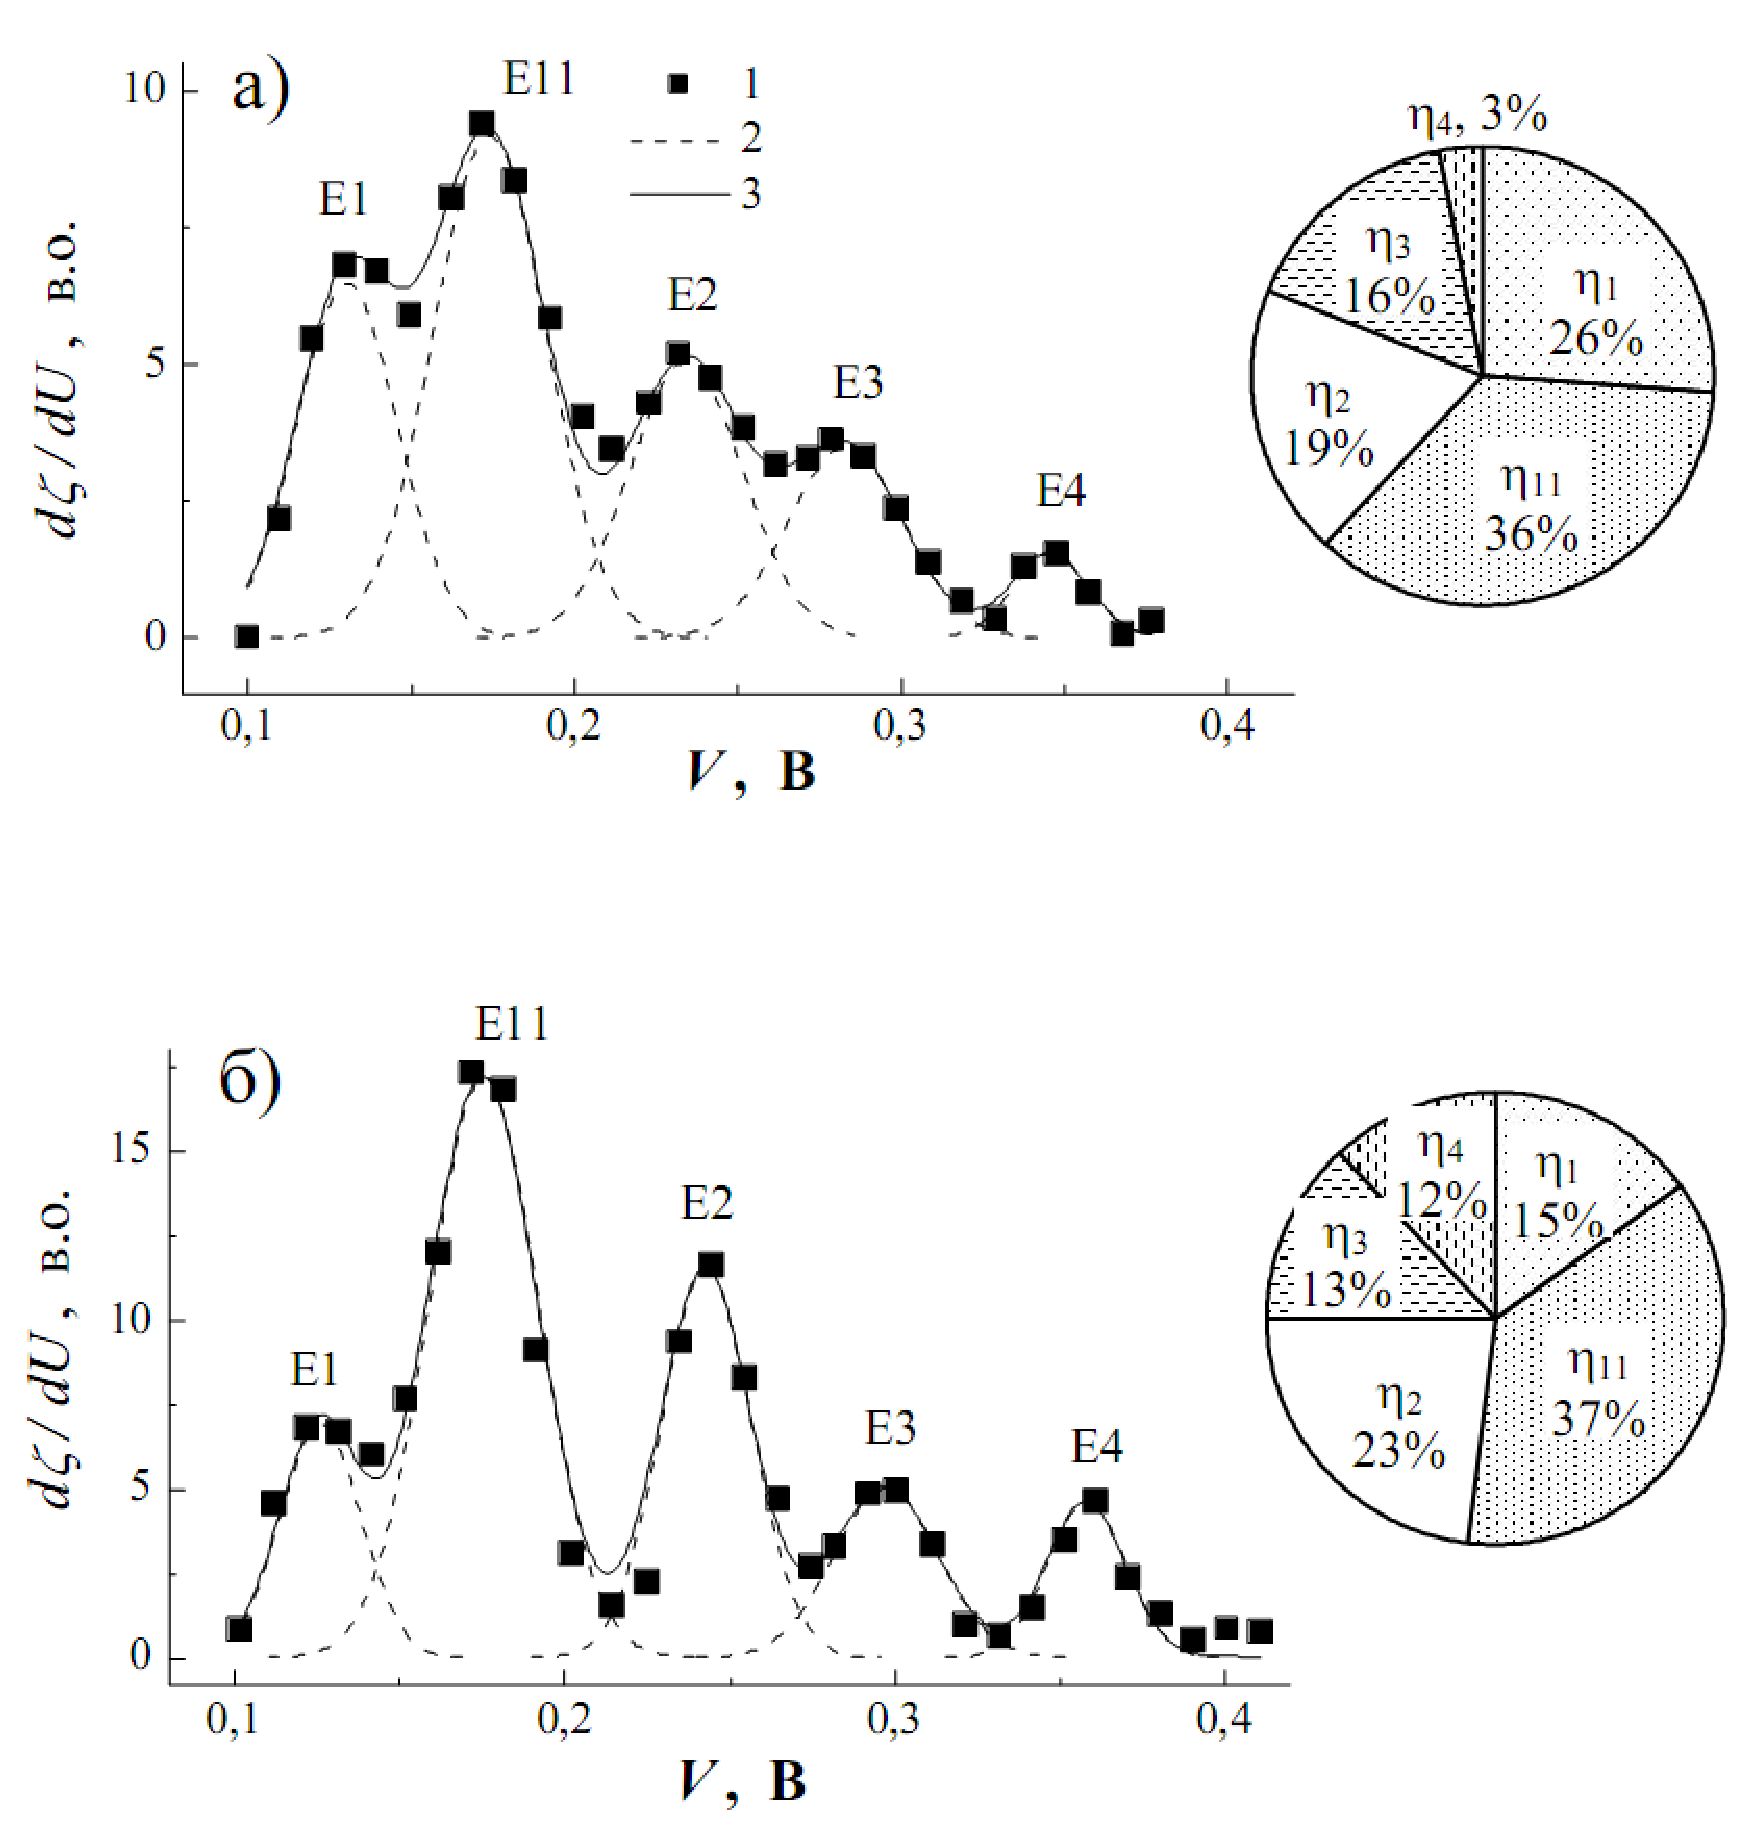
\includegraphics[width=1.0\textwidth]{figBul2}
\caption{\label{figBul2}
Польова залежність похідної диференційного показника нахилу ВАХ за відсутності УЗН (а)
та за його наявності (U--L4t,  $W_\mathtt{US}=0,60$~Вт/см$^2$, б).
1 --- точки, отримані після диференціювання експериментальних ВАХ,
2 --- гаусіани, якими апроксимувалися максимуми,
3 --- сума всіх гаусіан.
Зразок SC3.
Справа біля кривих наведено діаграми питомих внесків $\eta_i$ кожного з максимумів у загальну криву.
}%
\end{figure}

Загалом, в літературі відомо чимало дефектів в кристалах кремнію, енергетичні рівні яких знаходяться на відстані
$0,35\div0,50$~еВ від дна зони провідності.
Відомі значення енергій активації та відповідні конфігурації дефектів наведено в правій частині Таблиці~\ref{tabBulEtUSL}.
Спираючись на отримані величини $E_c-E_t$, технологію виготовлення зразків та літературні дані
визначемо, які конкретні дефекти можуть бути співставлені рівням Е1--Е4.

Досліджені структури містять несиметричний $n^+$--$p$ перехід і ОПЗ знаходиться практично повністю в області з дірковою провідністю.
Отже, переважно рекомбінація буде відбуватися за участю тих центрів, які мають донорний характер.
Як вже згадувалося, легування $n$--шару здійснювалось шляхом іонної імплантації фосфору.
В таких структурах, як в $n$--, так і в $p$--областях, можуть часто зустрічатися так званий Е--центр,
тобто комплекс вакансії та заміщуючого атома фосфору VP$_s$.
Цьому дефекту відповідає  рівень з енергетичним положенням $E_t=E_c-(0,42\div0,46)$~еВ \cite{VI:Luc,Karazh,Kuchinskii,Ecentre:2005}, що близько до параметрів центру Е2.
Проте відомо \cite{Kuchinskii,Ecentre:2005}, що цей рівень є акцепторним, йому відповідає зарядовий стан  $(-/0)$ і він є рекомбінаційно--активним переважно в $n$--Si.
Тому вважаємо, що Е--центр не відповідає за появу рівня Е2.
Після імплантації та відпалу атоми фосфору не зустрічаються у складі міжвузлових комплексів \cite{ChelyadFTT} і тому подібні дефекти ми також виключимо з розгляду.

Іншими типовими дефектами, які виникають внаслідок іонного опромінення є різноманітні
вакансійні комплекси.
Наприклад, енергія активації рівня Е1 0,48~еВ достатньо близька до положення рівня
комплексу COV$_2$  $E_t=E_c-0,475$~еВ \cite{Lugakov}.
Проте цей центр спостерігався в $n$--Si, опроміненому або електронами, або $\gamma$--квантами \cite{Lugakov} і тому його поява в досліджених структурах малоймовірна.

За своїм енергетичним положенням у верхній частині
забороненої зони рівні дивакансії $(-/0)$ $E_c-(0,43\div0,44)$~еВ \cite{V2:JAP2014,V2:PRB2002},
вакансії $(2-/-)$ $E_c-0,39$~еВ \cite{MSER55},
тривакансії $(2-/-)$ $E_c-(0,34\div0,36)$~еВ та $(-/0)$ $E_c-0,46$~еВ \cite{V3:PRB2012,V3:Markevich}
можуть відповідати центрам Е2, Е3, Е4 та Е11.
Проте всі вони є акцепторними (одно-- чи двозарядними) і тому також не можуть проявлятися
в наших експериментах.
Подібна властивість, коли акцепторні рівні знаходяться у верхній половині $E_g$,
а донорні --- в нижній, характерна і для різноманітних мультивакансій V$_n$ ($n>3$) \cite{Si:multiV}.

Утворені після імплантації фосфору вакансії є достатньо рухливими і в Cz--Si
утворюють (особливо після відпалу) комплекси з киснем \cite{V2toV2O}.
Глибина залягання рівня Е4 близька до розташування стану V$_3$O $(2-/-)$ (0,34~еВ нижче дна зона провідності \cite{V3:Markevich}),
а рівня Е11 --- до станів V$_3$O $(-/0)$ ($E_c-0,46$~еВ \cite{V3:Markevich})
та V$_2$O $(2-/-)$ ($E_c-0,46$~еВ \cite{V2:JAP2014}).
Проте ці рівні також акцепторні.
Таким чином, участь комплексів, пов'язаних з вакансіями, в утворенні
піків на залежності $\partial \zeta/ \partial V $, зв'язаних з рівнями Е1--Е4 може бути виключена.

При іонній імплантації кремнію, попередньо легованого бором,
у значній кількості утворюються власні міжвузольні дефекти та B$_i$.
Положення рівня міжвузольного бору $E_c-0,37$~еВ \cite{Bi:Harris} близьке до  енергії активації Е4.
Тоді як з Si$_i$ пов'язують декілька рівнів: $E_c-0,36$~еВ \cite{MSER55},
$E_c-0,39$~еВ \cite{MSER55,Si:Sii}, $E_c-0,43$~еВ \cite{Si:Sii} та
$E_c-0,44$~еВ \cite{VI:Luc}.
Зауважимо, що перший з них є нестабільним і спостерігається лише після опромінення при низьких температурах \cite{MSER55}.
Ці характеристики близькі до енергій активацій рівнів Е2 та Е4.

Раніше, у параграфі~\ref{sbDefectType}, вже згадувалося, що
типовими порушеннями в Cz--Si:B є ВО дефекти, кисневмісні преципітати та домішки заліза.
До речі, утворення КП також супруводжується емісією Si$_i$ \cite{MSER13}:
\begin{equation*}\label{eqSiO}
  2\,x\,\mbox{O}_i+y\,\mbox{Si}_s\leftrightarrows x\,\mbox{SiO}_2+(y-x)\,\mbox{Si}_i\,.
\end{equation*}
З самими КП пов'язують рівні, розташовані на відстані 0,41--0,43~еВ від дна зони провідності \cite{SiO:Mchedlidze,SiO:Vanhell,SiO:Chan}, що, враховуючи  $\delta_{Et}$, достатньо близько до енергії активації Е3.

Подібне розташування ($E_t=E_c-0,41$~еВ, \cite{LIDRev,LIDRev2,BO3i,Rein,LID:SchmidtJMR}) характерне і для ВО--дефекту.
Як відомо, ці центри утворюються внаслідок інжекції носіїв,
їх конфігурація визначена не точно, зокрема в літературі пропонується,
що це можуть бути комплекси B$_i$B$_s$O$_i$, B$_s$Si$_i$\cite{LIDRev} або
B$_i$O$_{3i}$ \cite{BO3i}.
Проте серед ВО виділяють дефекти,
що утворюються швидко (FRC, fast--formed recombination center)
та повільно (SRC, slow--formed recombination center).
Означений вище рівень відносять до SRC--форми,
тоді як  BO$_\mathtt{FRC}$ характеризується рівнем $E_c-(0,36\div0,38)$~еВ \cite{LIDRev2,BOSingle:SEMSS2017}, який
також потрапляє у діапазон, що нас цікавить (рівень Е4).

При утворенні КП, окрім власних міжвузольних атомів, для зняття механічних напруг також утворюються дислокації та дефекти пакування.
Серед останніх виділяють так звані OSFR--дефекти (oxidization induced stacking--faults ring), оточені кільцевими частковими дислокаціями \cite{MSER74,MSER28}.

З дислокаціями в кремнії пов'язують цілий ряд енергетичних рівнів, зокрема
$E_c-(0,37\div0,39)$~еВ \cite{PhysRevB56:10208,kveder2008,SiO:Hwang,disl10:Isakova,Kittler2003},
$E_c-0,43$~еВ \cite{PhysRevB56:10208,SiO:Vanhell}
$E_c-(0,50\div0,52)$~еВ \cite{Edis:Ogawa,Edis:Omling,Kittler2003},
близькі за параметрами до Е4, Е2 та Е1, відповідно.

Щодо рівнів, пов'язаних з дефектами, які містять залізо, то у діапазоні енергій, який розглядається,
знаходяться рівні $E_c-45$~еВ, пов'язаний з комплексом FeO \cite{FeO},
та $E_c-43$~еВ, що співставляється з парою Fe$_i$B$_s$, що має ромбічну симетрію \cite{FeB:PhysRevB49,Istratov1999}.
Як видно з даних Таблиці~\ref{tabBulEtUSL}, ці значення співрозмірні з енергією активації Е2.

Таким чином, серед типових дефектів у кремнієвих структурах є декілька кандидатів,
які можуть біти відповідальними за появу рівнів Е1, Е2, Е3 та Е4 та, фактично, жодного на роль Е11.
У наступному параграфі, спираючись на виявлені АІ ефекти, це коло буде звужене (розширене).

\subsection{Акусто--індуковані зміни в системі рекомбінаційних центрів\label{sbBul3}}

Як вже зазначалося, в умовах УЗН залежність $\partial \zeta/ \partial V = f (V)$ змінювалась.
Основні результати щодо впливу УЗН на рекомбінаційні рівні в SC11A та SC3 наведено
на Рис.~\ref{figEta1} та Рис.~\ref{figEta2}, відповідно.
Узагальнюючи представлені результати зазначимо, що


\begin{figure}
\center
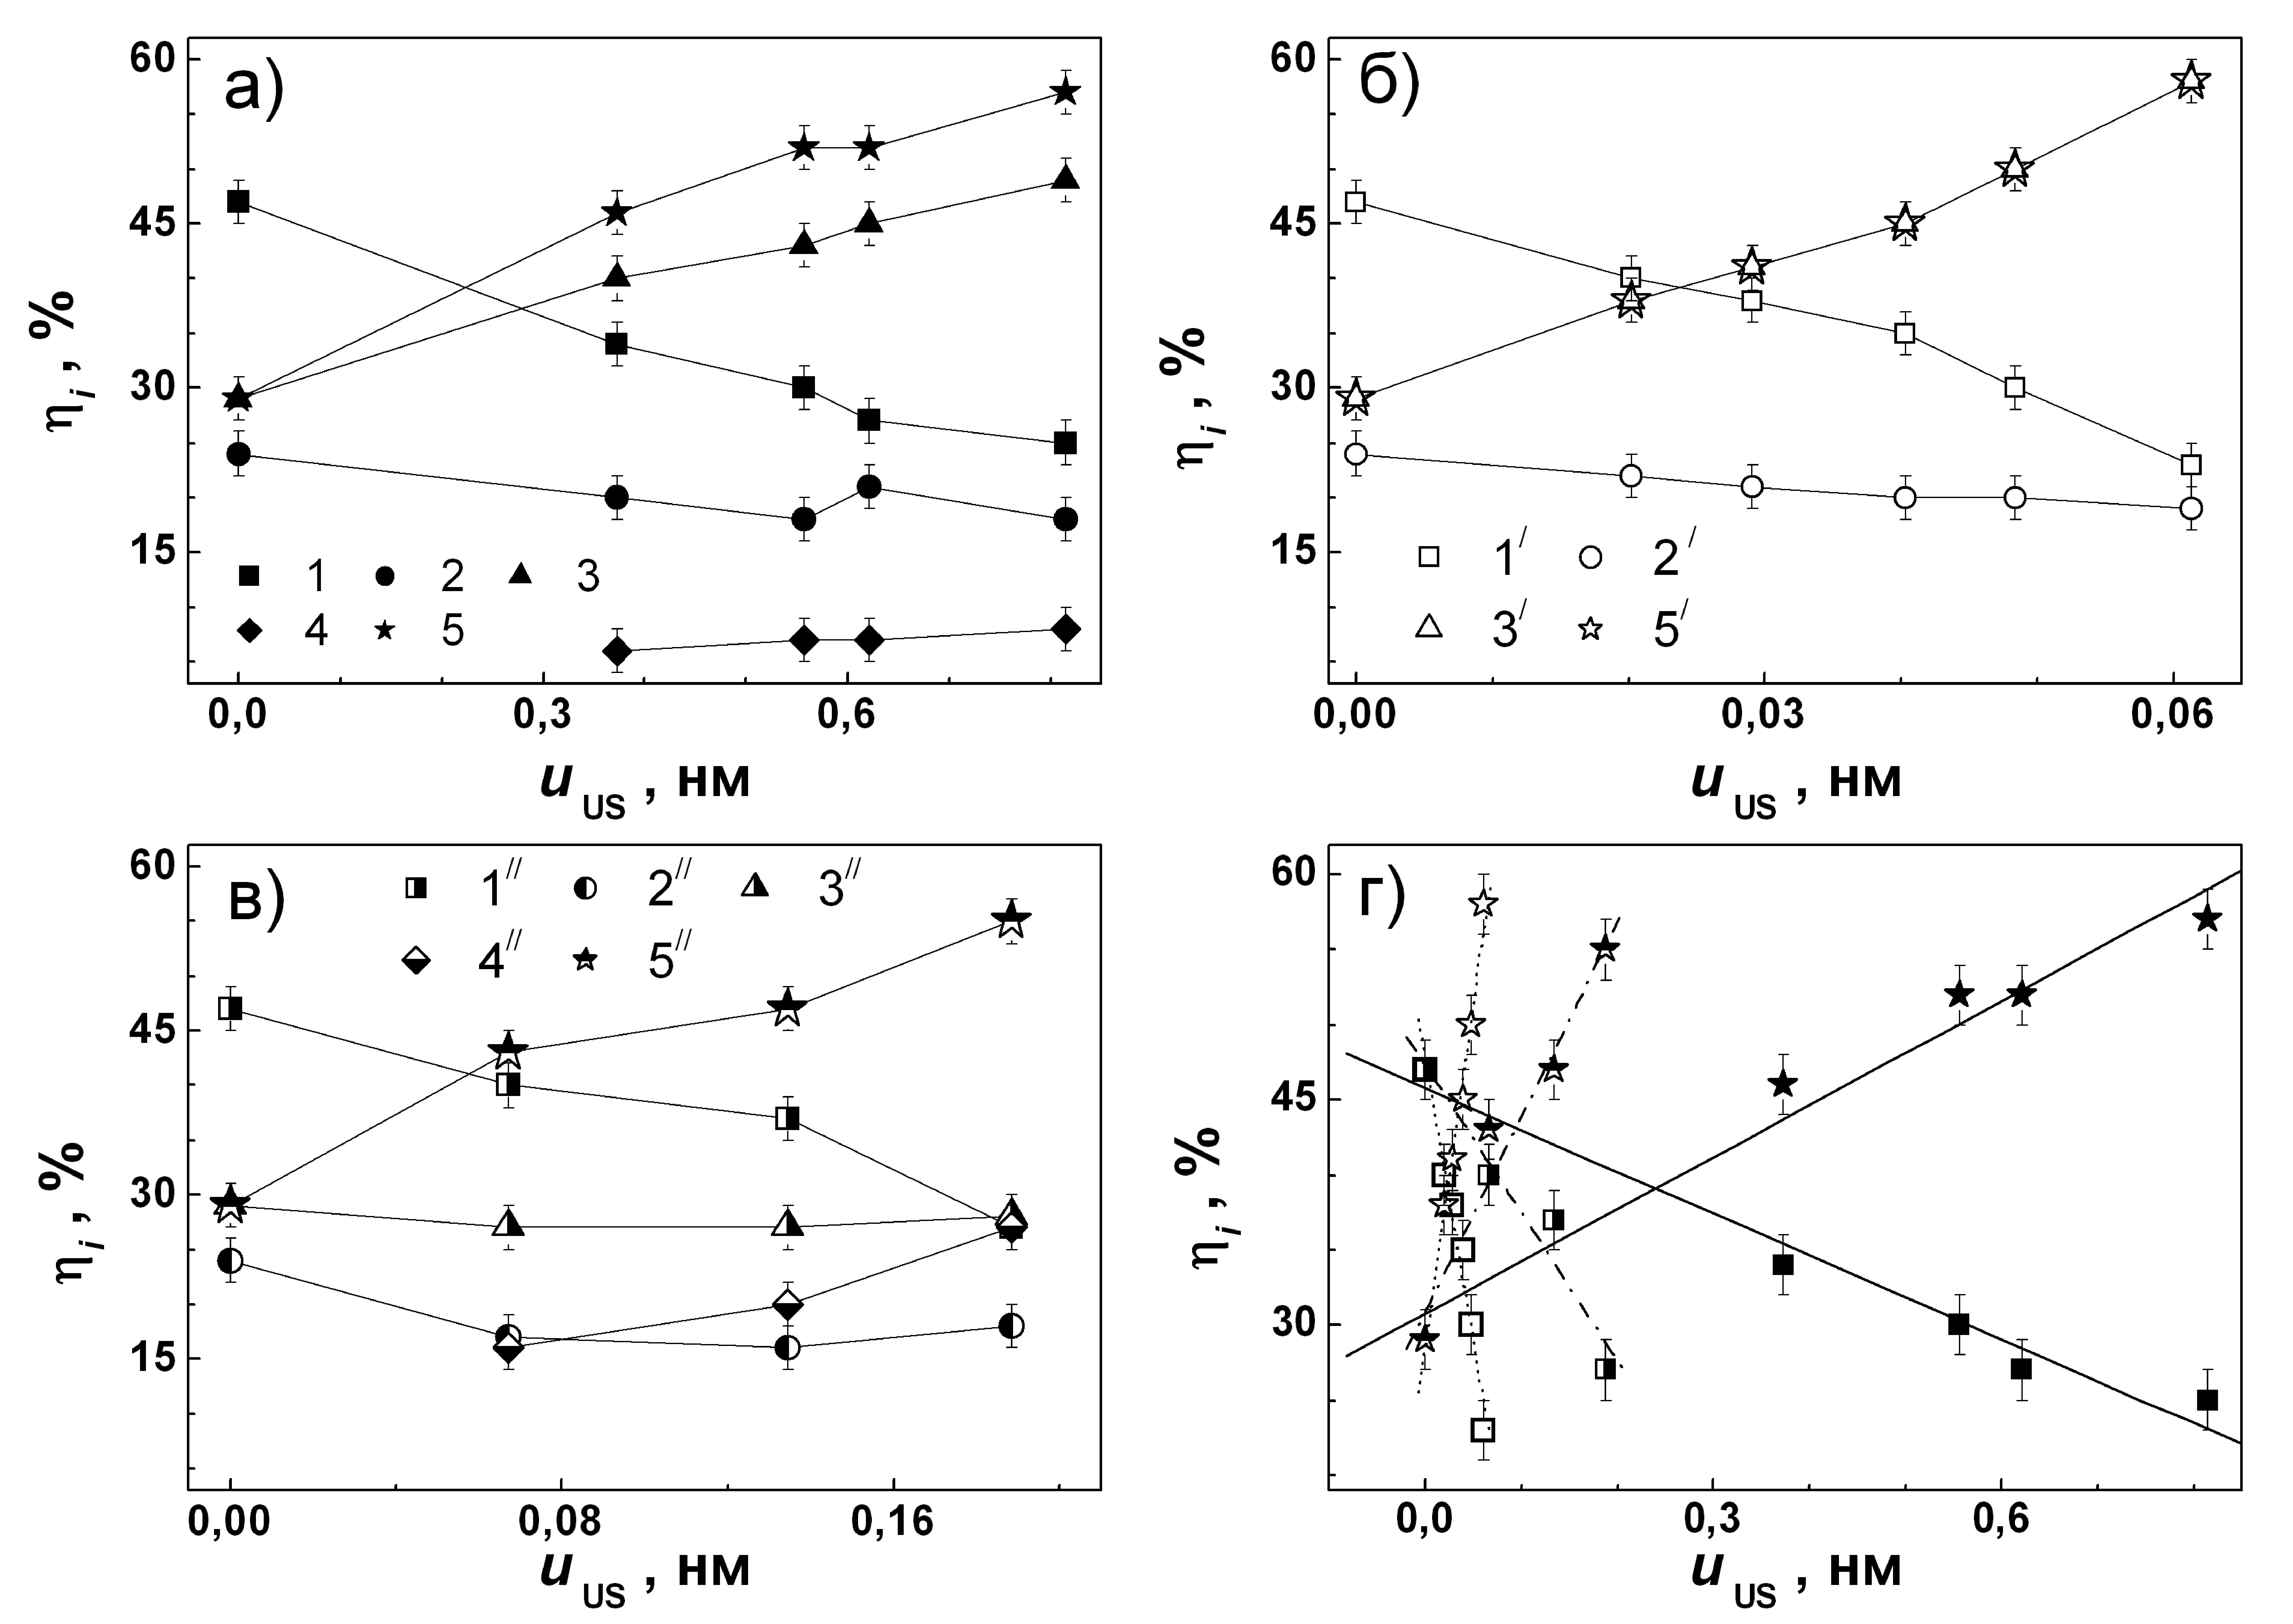
\includegraphics[width=1.0\textwidth]{figEta1}
\caption{\label{figEta1}
Залежність питомих внесків у загальну рекомбінацію рівнів
Е1 (криві 1, 1$^{\prime}$ та 1$^{\prime\prime}$, квадрати),
Е2 (криві 2, 2$^{\prime}$ та 2$^{\prime\prime}$, кола),
Е3 (криві 3, 3$^{\prime}$ та 3$^{\prime\prime}$, трикутники)
та Е4 (криві 4, та 4$^{\prime\prime}$, ромби),
а також сумарного внеску
Е3 та Е4 (криві 5, 5$^{\prime}$ та 5$^{\prime\prime}$, зірки)
від амплітуди зміщень атомів
при U--L4t (а, г, заповнені точки),
U--L26t (б, г, порожні точки),
U--L8t (в, г, напівзаповнені точки).
Зразок SC11A.
На а--в лінії наведені лише для зручності,
на г --- лінії результат лінійної апроксимації.
}%
\end{figure}

\begin{figure}
\center
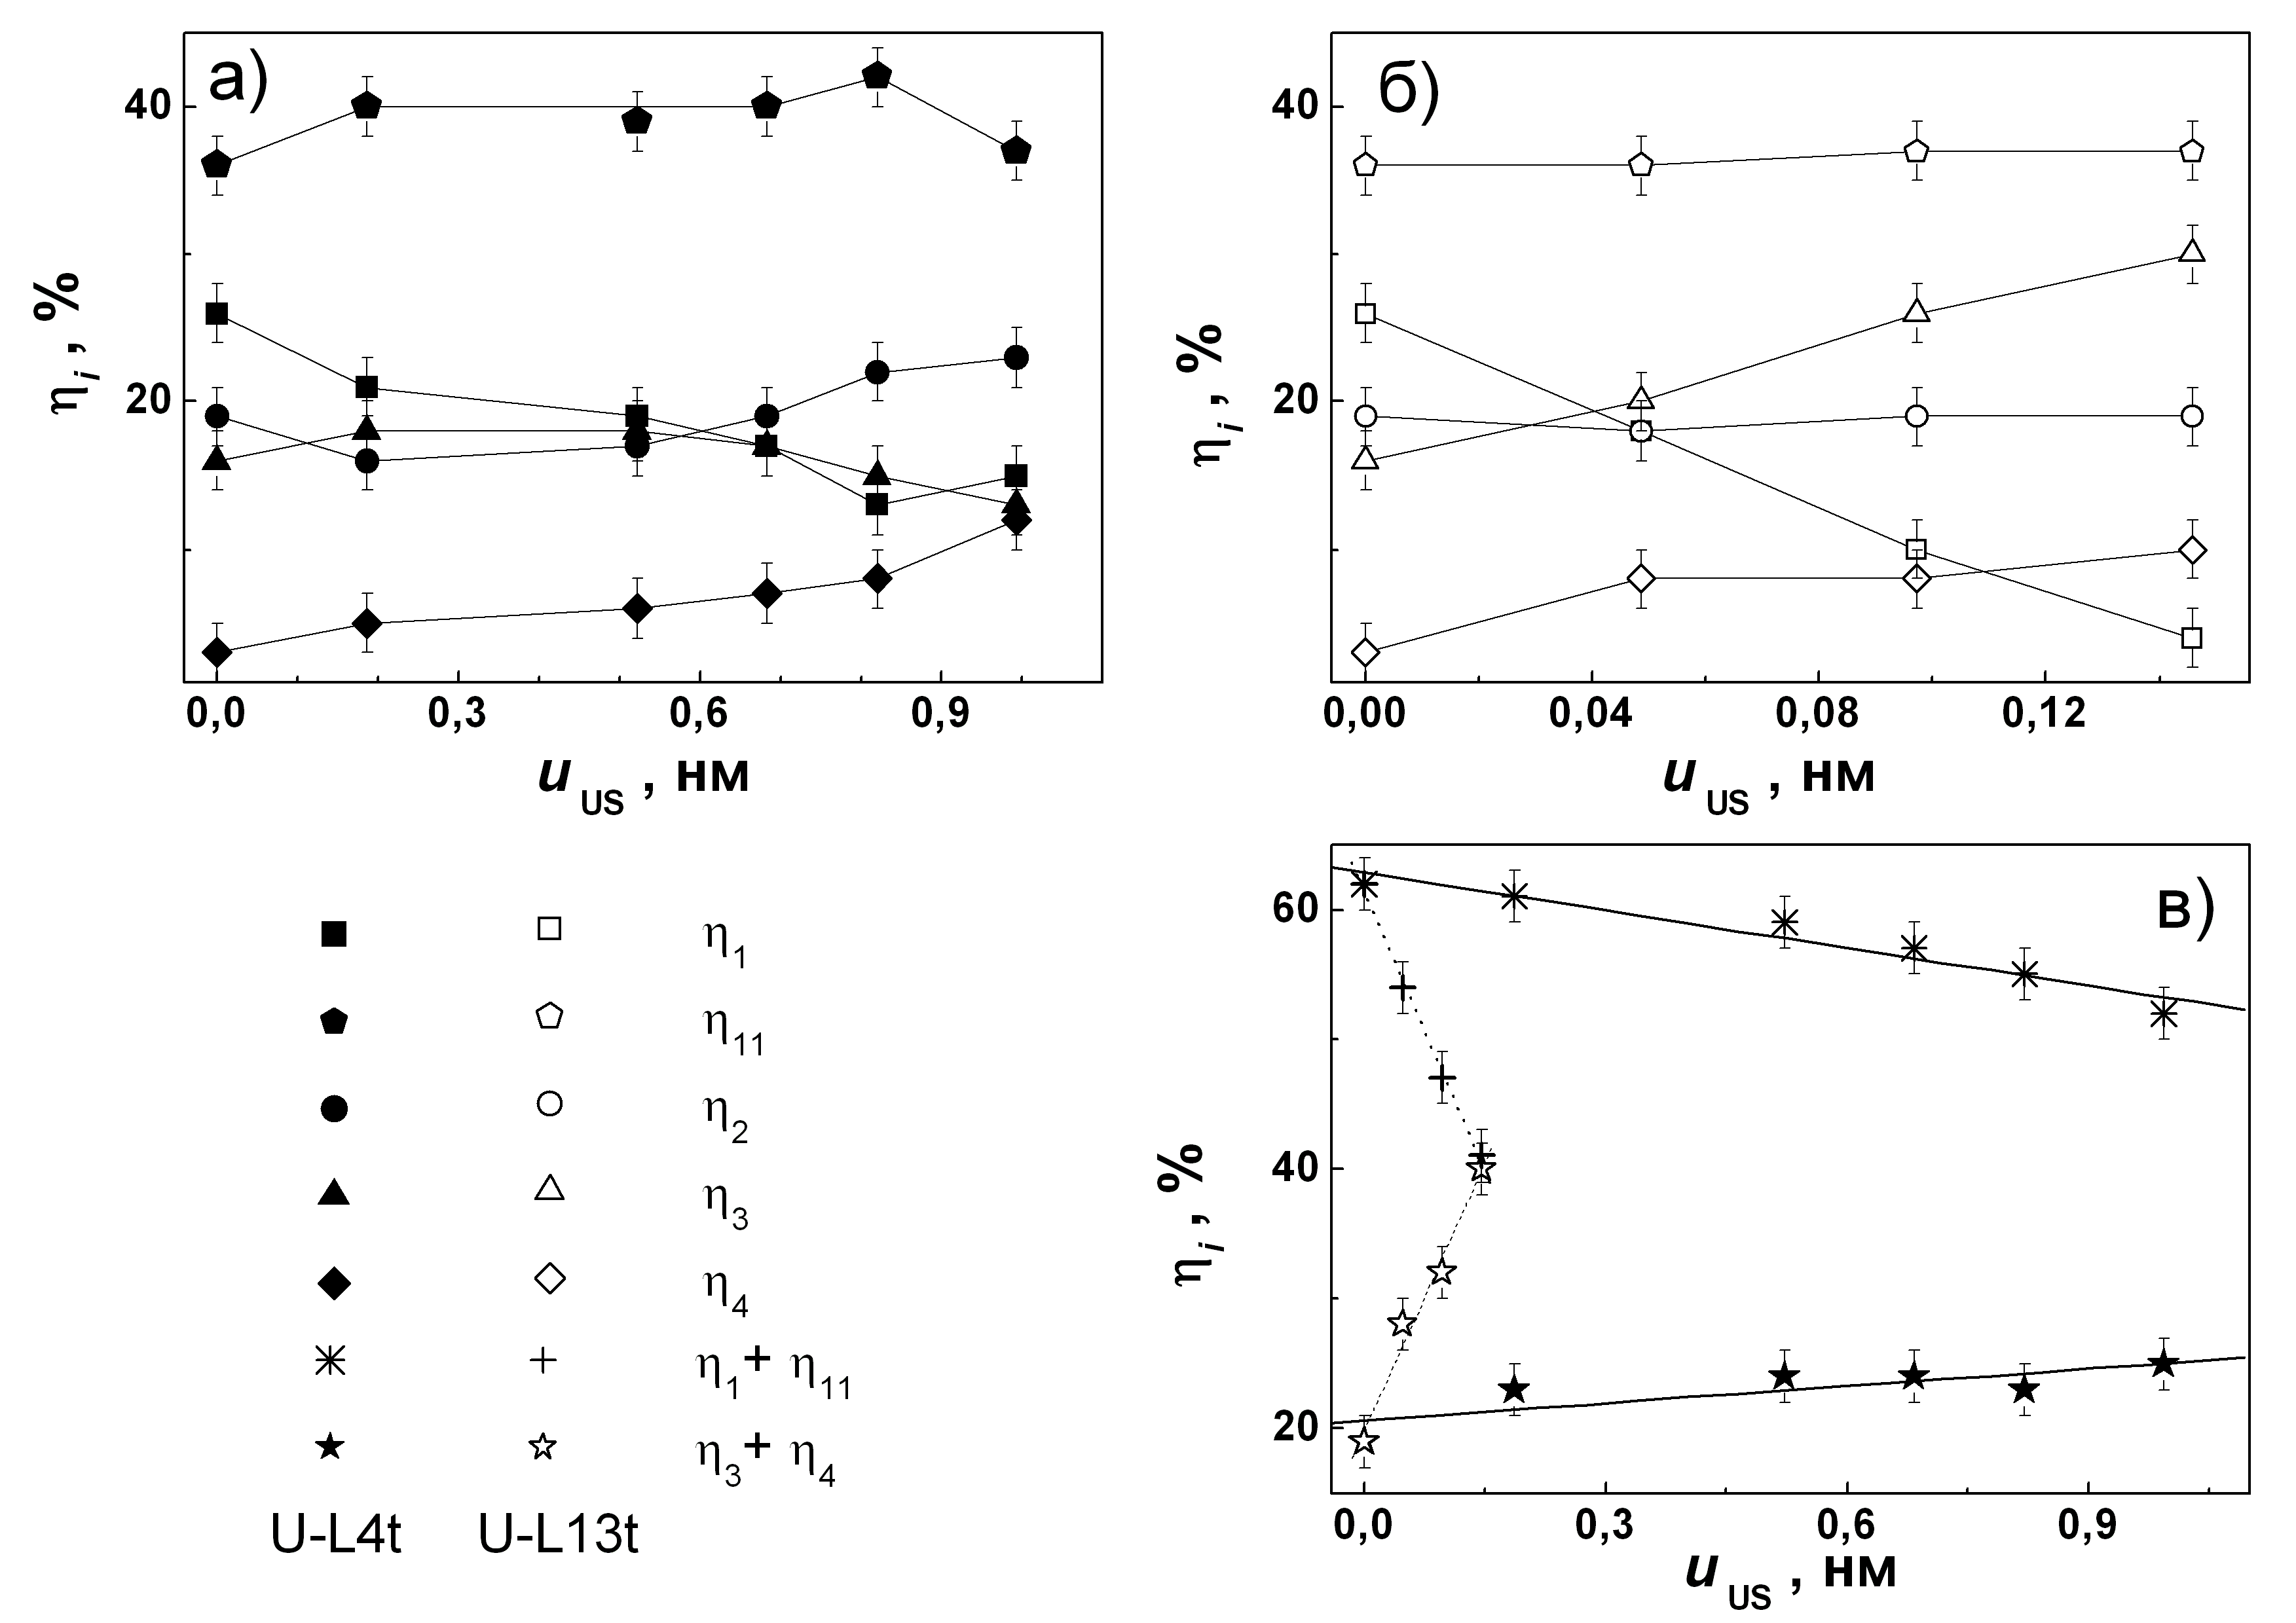
\includegraphics[width=1.0\textwidth]{figEta2}
\caption{\label{figEta2}
Залежність питомих внесків у загальну рекомбінацію рівнів
Е1 (квадрати),
Е11 (п'ятикутники),
Е2 (кола),
Е3 (трикутники)
та Е4 (ромби),
а також сумарного внеску
Е1 та Е11 (хрести) і
Е3 та Е4 (зірки)
від амплітуди зміщень атомів
при U--L4t (а, в, заповнені точки) та
U--L13t (б, в, порожні точки).
Зразок SC3.
На а--в лінії наведені лише для зручності,
на г --- лінії результат лінійної апроксимації.
}%
\end{figure}

\begin{enumerate}[label=\asbuk*),leftmargin=0em,itemindent=1.5em]
\item зі збільшенням інтенсивності УЗ збільшується роль у рекомбінаційних процесах рівнів, розташованих ближче до дня зона провідності; зокрема збільшується внесок рівня Е3 та зменшується внесок рівня Е1, причому залежності показників питомого внеску рівнів від амплітуди зміщень атомів у  АХ ($\eta_i\sim U_\mathtt{US}$);
\item АІ зміни відбуваються більш ефективно при підвищенні частоти УЗН --- див Рис.~\ref{figEta1},г та Рис.~\ref{figEta2},в;
\item в умовах УЗН в зразку SC11A з'являється сигнал від ще одного ГР (Е4), тоді як в SC3 відповідний сигнал наявний і за відсутності пружних коливань; внесок цього рівня $\eta_4$ збільшується зі зростанням $U_\mathtt{US}$;
\item спостерігається незначний, 0,010--0,015~еВ, зсув положення рівнів ближче до дна зони провідності; зауважимо що величина зсуву співрозмірна з похибкою визначення енергії активації і причиною виокремлення цього ефекту є лише постійність його знаку для всіх зразків та режимів.
\end{enumerate}

Зупинимось на причинах АІ появи рівня Е4.
У випадку, коли цей рівень пов'язаний з міжвузольним атомом бору, можна запропонувати наступним механізм цього ефекту.
При УЗН може відбуватися звільнення власних міжвузольних атомів, захоплених дислокаційними петлями поблизу $p$--$n$ переходу (можливість існування значної кількості Si$_i$ та дислокацій згадувалась у попередньому параграфі);
після цього Si$_i$ дифундують в глибину $p$--області, де витісняють легуючі атоми В з вузлів за механізмом Воткінса.
Проте
а)~при такому варіанті незрозумілим залишається зникнення сигналу від Е4 в SC11A після припинення УЗН (всі виявлені ефекти є оборотними);
б)~В$_i$ є центром з від'ємною кореляційною енергією, його донорний рівень $E_t=E_c-0,13$~еВ \cite{Bi:Harris} знаходиться ближче до $E_c$, тому ймовірність спостереження акцепторного рівня
$E_t=E_c-0,37$~еВ в $p$--Si дуже мала;
в)~дефект відпалюється вже при температурах 240--250~K, перетворюючись на комплекс B$_i$O$_i$ ($E_c-0,23$~еВ) \cite{PhysRevB94}.
Як наслідок, подібний механізм, як і те, що Е4 пов'язаний саме з В$_i$, видається малоймовірним.

Інший цікавий з точки зору АДВ варіант появи Е4 полягає в тому, що в умовах УЗН відбувається
перебудова ВО дефекту з однієї конфігурації в іншу: $\mbox{BO}_\mathtt{CRC} \rightarrow \mbox{BO}_\mathtt{FRC}$.
Тобто і Е3, і Е4 відносяться до одного й того ж ВО дефекту у різних конфігураціях,
УЗН викликає збільшення частки дефектів у конфігурації  BO$_\mathtt{FRC}$, що призводить до появи відповідного максимуму (SC11A) або його підсилення (SC3).
Те, що сигнал від Е4 присутній у SC3 і до УЗН свідчить просто про нерівномірність розподілу цих дефектів по пластині.
Якщо Е3 та Е4 відповідають двом станам ВО, то доцільно розглядати суму $\eta_3+\eta_4$ як показник внеску цього дефекту в загальну рекомбінацію, що і зроблено на рисунках.
Отримані залежності вказуються, що в цілому внесок ВО комплексу в рекомбінацію при дії пружних коливань зростає.
Як було розглянуто раніше (параграф~\ref{sbAEDefect}), згідно з моделлю акусто--активного комплексу найбільш очікуваною АДВ є для системи, складові якої характеризуються різним за знаком надлишковим об'ємом.
В цілому, ВО задовольняє цій умові для конфігурацій, що містять заміщуючий атом бору (B$_i$B$_s$O$_i$ тв B$_s$Si$_i$).
Дійсно, так як ковалентний радіус бору дорівнює 0,8~{\AA}, а кремнію -- 1,18~{\AA},
то $\Delta\Omega_d\,(\mbox{B}_s)<0$,
тоді як для міжвузольних компонент $\Delta\Omega_d>0$.

На жаль, від такої стрункої картини доведеться також відмовитися.
По--перше, з недавнього часу в літературі наводяться докази того, що не існує двох
різних конфігурацій  (двох різних дефектів) FRC та SRC \cite{BOSingle:Voronkov,BO3i,BOSingle:SEMSS2017,Kim},
а отже АІ перехід $\mbox{BO}_\mathtt{CRC} \rightarrow \mbox{BO}_\mathtt{FRC}$ неможливий.
По--друге, згідно з результатами, викладеними в параграфі~\ref{sbDefectType},
в досліджуваних зразках ВО центри не впливають на рекомбінацію,
а отже ні Е3, ні Е4 з ВО дефектами не зв'язані.


На наш погляд, правильна картина АІ появи E4 наступна.
Відомо, що на периферійних ділянках напівпровідникових пластин концентрація дефектів вища,
ніж для центральних.
В нашому випадку про це, зокрема, свідчить менше значення шунтуючого опору в ($\sim2\cdot10^{3}$~Ом при кімнатній температурі) порівняно з SC11А ($\sim2\cdot10^{4}$~Ом).
В досліджуваних структурах шунтуючий опір визначається дислокаціями, які перпендикулярні до площини $p$--$n$ переходу, причому в умовах УЗН їх рекомбінаційна активність зростає ($R_{sh}$ зменшується) --- детально це описано в параграфі~\ref{sbRsh}.
Якщо припустити, що Е4 зв'язаний з дислокаціями (див. Таблицю~\ref{tabBulEtUSL}), яких більше в SC3, то зрозумілим стає наявність відповідного максимуму в цьому зразку без УЗН і зростання $\eta_4$ при УЗН.

Щодо рівня Е3 (для якого $\eta_3$ також збільшується при поширенні АХ),
то він має бути пов'язаний з КП SiO$_x$.
Дійсно, згідно з результатами, представленими в параграфах \ref{sbQNR} та \ref{sbDefectType},
саме кисневмісні преципітати наявні в досліджених структурах і підвищують свою рекомбінаційну активність під дією УЗ.

Повертаючись до співставлення виявлених рівнів з конкретними дефектами зауважимо,
що Е1 може бути пов'язаний з OSFR та відповідними частковими дислокаціями.
Відомо, що при захопленні дислокаціями домішок, їх рекомбінаційна активність
збільшується у декілька разів \cite{disl10:Kveder,Kittler2003}.
При УЗН відбувається часткове звільнення цих захоплених атомів, що і викликає
зменшення  $\eta_1$.
Крім того, в літературі описано уширення  лінії дислокаційної люмінесценції внаслідок захоплення домішки  \cite{PhysRevB56:10208}.
Більш висока концентрація домішок в SC3, у тому числі і захоплених на дислокаційні петлі,
на нашу думку і викликає наявність в діапазоні $E_c-(0,46\div0,48)$~еВ двох рівнів (Е1 та Е11),
внесок яких в рекомбінацію суттєво вищий, ніж в SC11А --- див. Рис.~\ref{figBul1} та Рис.~\ref{figBul2}.
Отже, внесок цих рівнів в рекомбінаційні процеси також можна розглядати разом ($\eta_1+\eta_{11}$, див. Рис.~\ref{figEta2}).

В параграфі \ref{sbDefectType} також було показано, що в ОПЗ присутні також домішкові атоми заліза.
Саме з ними і пов'язаний рівень Е2.
Вибираючи між Fe$_i$B$_s$ та Fe$_i$O$_i$ (див. Таблицю~\ref{tabBulEtUSL}), врахуємо наступне.
Звичайно, найчастіше як рекомбінаційний центр розглядають пару залізо--бор,
проте в літературі показано, що в $n^+-p$ переходах активними можуть бути і інші
залізовмісні пастки \cite{TeimurazPSS,TeimurazJAP}.
Пара  Fe$_i$B$_s$ є бістабільною, може перебувати в двох конфігураціях, які відрізняються відстанню між компонентами комплексу на симетрією (тригональна або ромбічна).
Рівень, з яким ми можемо пов'язати Е2, відповідає неосновному стану Fe$_i$B$_s^\mathtt{orth}$, тобто концентрація дефектів саме в цій конфігурації за рівноважних умов досить низька.
Нарешті, Е2 фактично не змінює свою рекомбінаційну активність в умовах УЗН.
$\Delta\Omega_d\,(\mbox{B}_s)<0$, то $\Delta\Omega_d\,(\mbox{O}_i)>0$, тобто комплекс
Fe$_i$B$_s$ є потенційно акусто--активним центром, тоді як для Fe$_i$O$_i$
$\Delta\Omega_d\,(\mbox{Fe}_i)\cdot\Delta\Omega_d\,(\mbox{O}_i)>0$.
Таким чином, кращим кандидатом для Е2 виглядає комплекс Fe$_i$O$_i$.

Наприкінці зауважимо, що зменшення енергії активації в кремнієвих структурах за умов
УЗ навантаження спостерігалося і раніше як для центрів, пов'язаних з дислокаціями \cite{KorotchFTP1996}, так і з точковими дефектами \cite{Korotchenkov1995}.
Причому в останньому випадку автори пов'язували ефект зі зміщенням домішки з рівноважного положення під дією механічної напруги, яка виникає під час поширення УЗ.


Таким чином, приведені результати підтверджують практичну перспективність динамічного акустичного керування властивостями напівпровідників та характеристиками приладів на їх основі.
Необхідно зауважити, що нерівноважний стан дефектів (в нашому випадку рекомбінаційних центрів), який виникає при появі нерівноважних носіїв заряду,
є важливим фактором підвищення ефективності АДВ загалом.
Саме в такому випадку додаткова коливальна деформація зовнішнього УЗ стає більш ефективним засобом керування характеристиками приладу.
Безумовно, питання фізичного механізму акустоіндукованих перетворень структури, конфігурації, зарядового стану дефектів у напівпровідниках потребують подальших досліджень.



\section{Особливості акусто--дефектної взаємодії в радіаційно--опромінених кремнієвих структурах з p--n переходом\label{Rad_SSC}}
У цьому параграфі викладено результати дослідження впливу УЗН на параметри опромінених кристалічних КСЕ.
Зрозуміло, що властивості таких структур визначаються, насамперед, дефектним складом.
Ефективність АДВ залежить від структури дефектів \cite{UST:Medvid} і
далеко не всі дефекти кристалічної структури кремнію є акусто--активними і здатні змінювати свою конфігурацію в умовах УЗН.
Одним з найбільш поширених та вивчених способів зміни дефектної підсистеми напівпровідників є опромінення.
З точки зору АДВ, з одного боку, виявлено \cite{YOlikh2007TPLr,Parchinskii2006r,Gorb2010,Podolian2012r}, що високоінтенсивна УЗО
здатна незворотнім чином змінювати властивості опромінених кремнієвих структур.
Цей ефект пов'язаний з АІ відпалом РД, насамперед точкових.
З іншого боку, опромінення може бути причиною появи оборотних АІ явищ \cite{YOlikh2006TPLr,YOlikhTPL2011r},
яка пов'язана з формуванням акусто--активних РД.
На жаль, експериментальному  дослідженню акусто--керованих ефектів в опромінених кремнієвих структурах присвячено достатньо небагато робіт.
Представлені результати частково доповнюють картину АДВ в подібних системах.
Зокрема проведено порівняння АІ ефектів, яки виникають при використанні опромінення різного типу (нейтронів та гамма--квантів),
а отже при появі дефектів різного типу.
Так як наслідки опромінення кремнію вивчені достатньо добре, то вдалося, зокрема, вирізнити
вплив УЗ на різні за типом РД.
Зразки та деталі радіаційного впливу описані у параграфі~\ref{SSC}.

Проводилось вимірювання ВАХ зразків у темряві за умов УЗН та без нього, спираючись на які було визначено параметри КСЕ.
Загалом процедура, за винятком об'єкту безпосереднього експериментального дослідження,
збігалася з описаною у параграфі~\ref{sbSSCMethod}.
Відмінності мали місце лише при отриманні результатів, наведених у параграфі \ref{sbNIsc},
але на його початку експериментальні деталі описані окремо.
На Рис.~\ref{figSSCIV2} наведено декілька прикладів виміряних кривих, які відображають
зміну форми ВАХ внаслідок опромінення.
Крім того, на рисунку за допомогою розривних ліній показано приклад розрахованих під час апроксимації внесків $I_{SCR}$, $I_{base}$ та $I_{sh}$
(див. формулу~(\ref{eqSSCIV})) у загальний струм.
На цьому рисунку, як і надалі, проводиться порівняння результатів,
отриманих для опромінених КСЕ, з даними для неопроміненого зразка SC11, параметри якого, зокрема величина шунтуючого опору,
схожі з параметрами SC4, SC8, SC12.
Так як при вивченні АІ ефектів в опромінених структурах використовувалися лише поперечні АХ,
то для порівняння наведено результати впливу на SC11 УЗН з таким самим типом хвиль.

\begin{figure}
\center
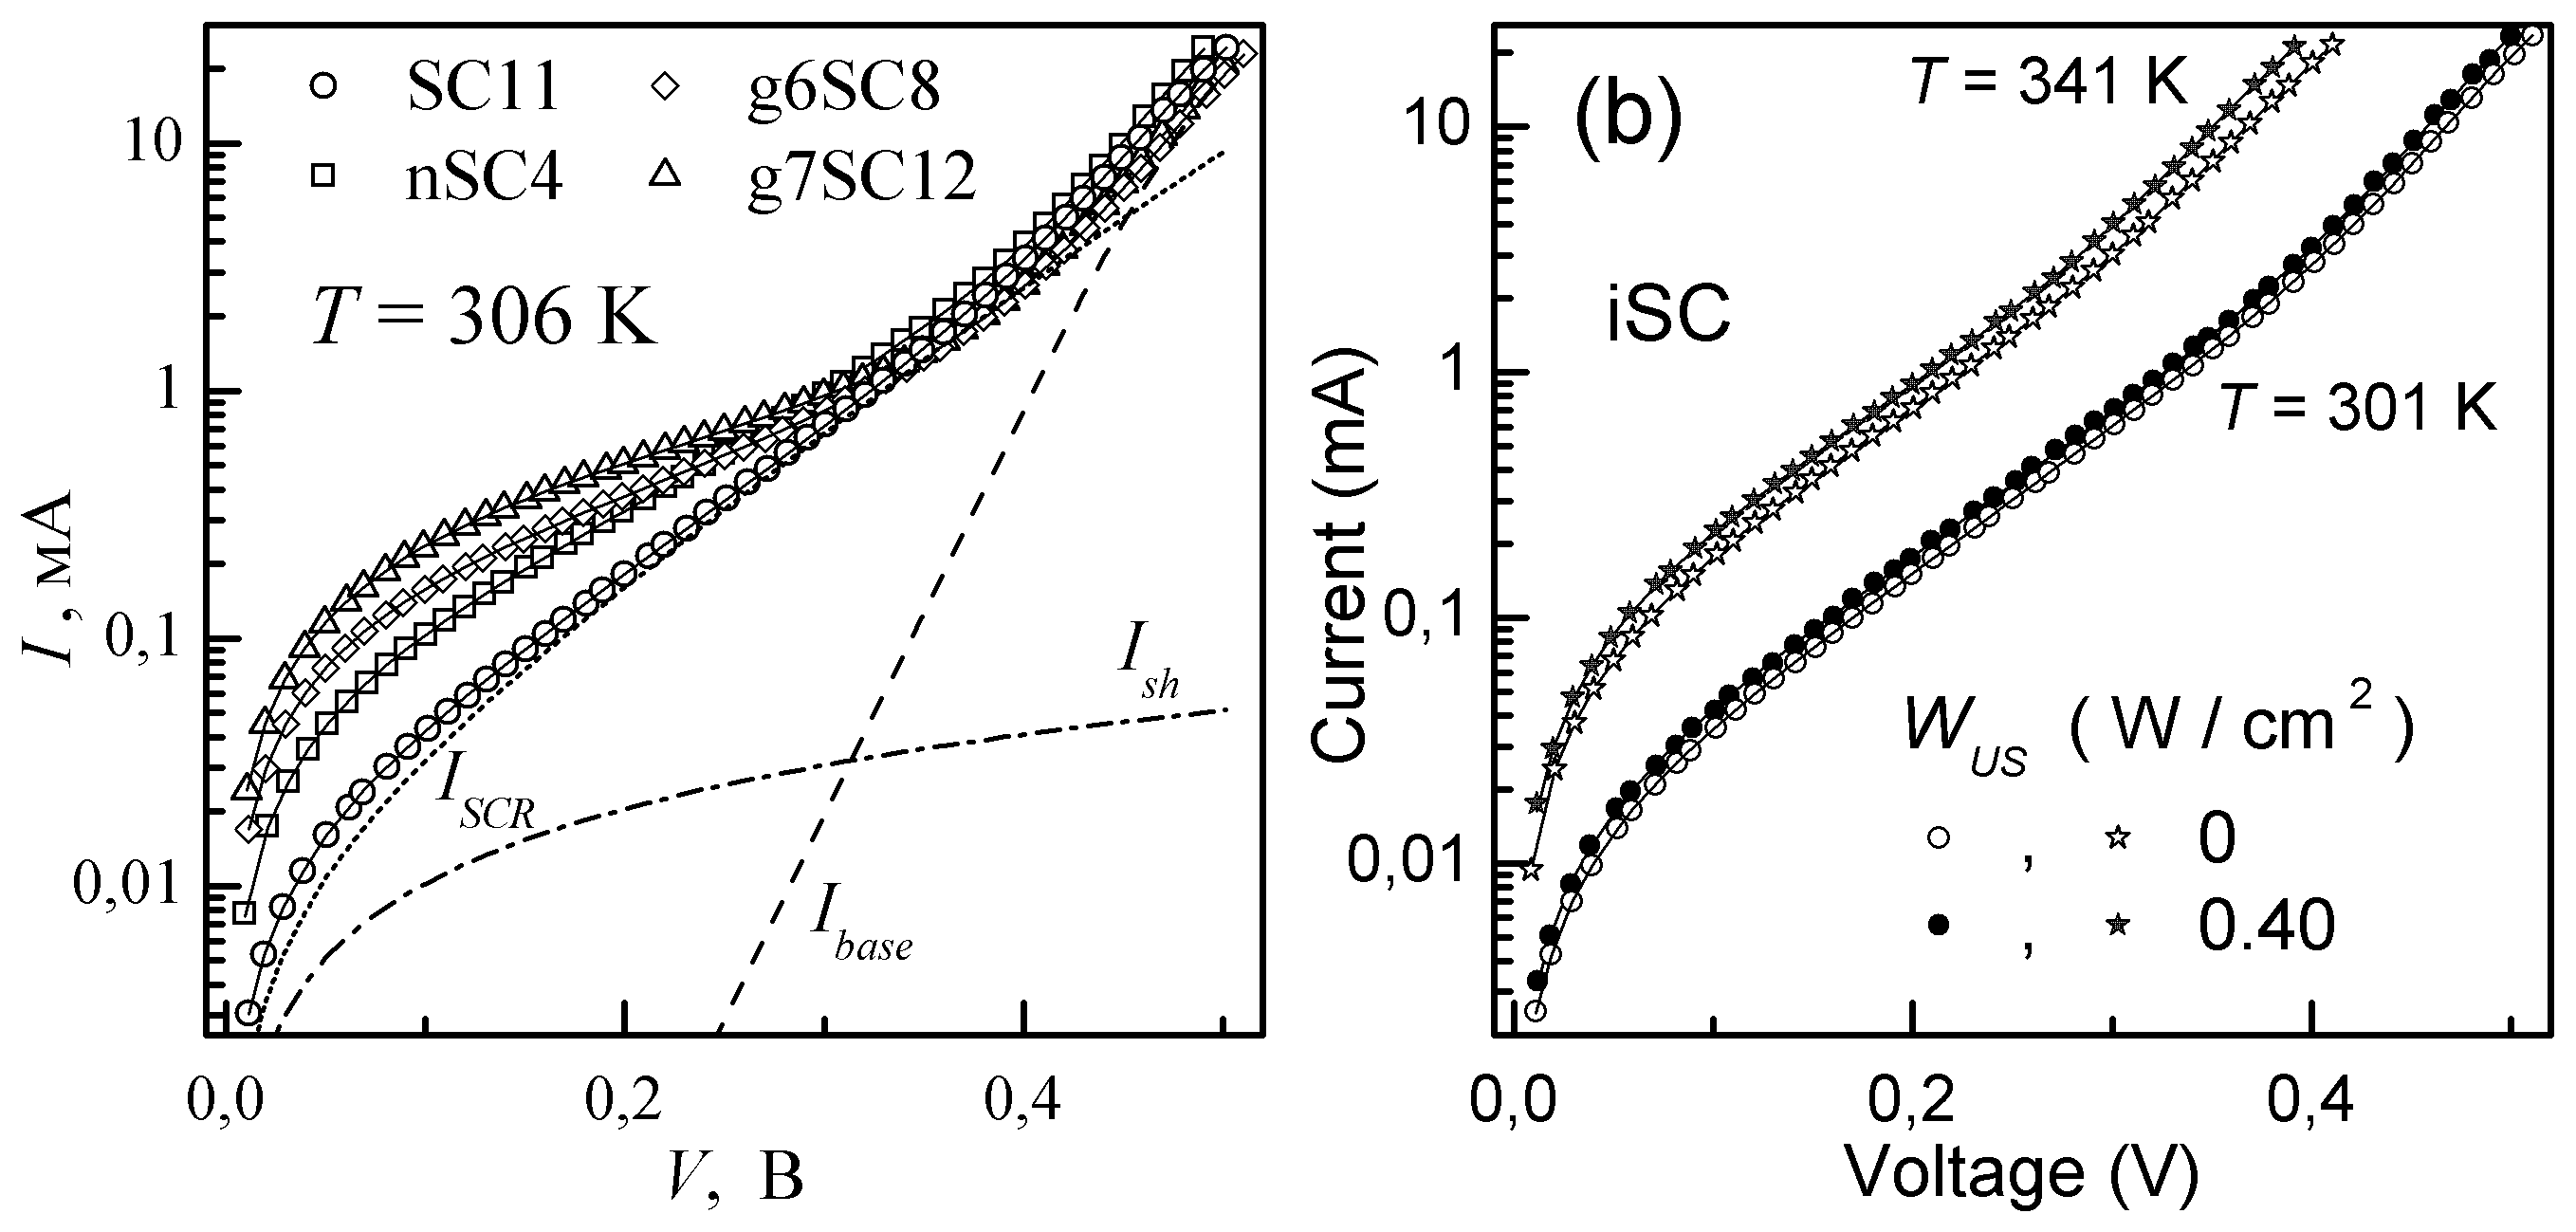
\includegraphics[width=0.6\textwidth]{figSSCIV2}%
\caption{\label{figSSCIV2}
Темнові ВАХ неопроміненого зразка (кола), нейтронно--опроміненого (квадрати) та $\gamma$-опроміненого (ромби та трикутники) виміряні при температурі 306~K без УЗН.
Точки відображають результати вимірів, лінії отримані шляхом апроксимації за формулами (\ref{eqSSCIV}) та (\ref{eqW}).
Штрихованою, пунктирною та штрих--пунктирною лініями показано розраховані складові повного струму, пов'язані з рекомбінаціяєю в КНО, в ОПЗ та шунтуючу складову, відповідно,
для неопроміненого зразка.
}%
\end{figure}



\subsection{Оцінка наслідків опромінення\label{sbRadDefCreate}}

При передбаченні структури РД, які утворюються внаслідок опромінення кристалів кремнію,
необхідно враховувати рівень та тип легування, концентрацію кисню та дозу.
В нашому випадку використовувалися зразки $p$--Si з концентрацією бору $\sim10^{15}$~cm$^{-3}$,
вирощені за методом Чохральського, зі значною концентрацією
кисню, $\sim7\times10^{17}$~см$^{-3}$ та достатньо низькі дози опромінення.
В цьому випадку очікується \cite{n:long,n:gamma,Moll:PhD}, що при нейтронному опроміненні будуть виникати
К--центри (пара міжвузольний вуглець--міжвузольний кремній, C$_i$O$_i$ ),
вакансійні кластери V$_n$ (дивакансії V$_2$, тривакансії V$_3$, ...) та
А--центри (пара вакансія--міжвузольний атом кисню, VO$_i$).
В той же час $\gamma$--промені мають викликати появу лише, переважно, C$_i$O$_i$ та VO$_i$ \cite{gamma:Stahl,Moll:PhD,gamma:Kolkr,A:Caracas}.
Відомо, що концентрація РД $N_{t,\mathtt{RD}}$ лінійно залежить від дози (флюєнсу) опромінення:
\begin{equation}
\label{eqNtRD}
    N_{t,\mathtt{RD}}=\vartheta^{D} D=\vartheta^{\Psi}\Psi \,,
\end{equation}
де $\vartheta^{D}$ ($\vartheta^{\Psi}$) --- швидкість введення (генерації) дефектів.
Запропоновані в літературі значення темпів генерації при опроміненні нейтронами $\vartheta_n$ та гамма--квантами $\vartheta_\gamma$
наведено в Таблиці~\ref{tabDefectNt}.
В цій же таблиці також наведені очікувані значення $N_{t,\mathtt{RD}}$ для досліджених зразків.

\begin{table}
\caption{\label{tabDefectNt}Швидкості введення та концентрації дефектів у досліджених зразках.
}
\center
\begin{tabular}{|c|c|c|c|c|c|c|}
\hline
Дефект&$\vartheta_n^{\Psi}$,  &$\vartheta_\gamma^{\Psi}$,&$\vartheta_\gamma^D$,&\multicolumn{3}{c|}{$N_{t,\mathtt{RD}}$, 10$^{11}$~см$^{-3}$}\\
\cline{5-7}
&см$^{-1}$ \cite{Moll:PhD}&см$^{-1}$ \cite{gamma:Kolkr}&рад$^{-1}$см$^{-3}$ \cite{gamma:Stahl}&nSC4&g6SC8&g7SC12\\
\hline
C$_i$O$_i$&1.38&4$\cdot$10$^{-4}$&6$\cdot$10$^5$&5,5&6&60\\ \hline
V$_2$&1,21&&3$\cdot$10$^4$&4,8&0,3&3\\ \hline
V$_3$&0,37&---&---&1,5&---&---\\ \hline
VO$_i$&0,52&4$\cdot$10$^{-4}$&7$\cdot$10$^5$&2&6--7&60--70\\\hline
\end{tabular}
\end{table}

У таблиці представлені дані лише для основних дефектів.
Окрім них при $\gamma$-- та нейтронному опроміненні кремнію можуть також утворюватися
а)~I$_p$ центри, пов'язані з міжвузольними атомами;
б)~бістабільні донори (BD-дефекти);
в)~пари міжвузольний бор--міжвозольний кремній (B$_i$O$_i$);
г)~пари міжвузольний вуглець--заміщуючий вуглець (C$_i$C$_s$).
Проте в досліджуваних зразках їх впливом можна знехтувати.
Так, утворення бістабільних донорів та I$_p$ центрів характеризується порівняно малою швидкістю введення.
Наприклад, як показують результати робіт \cite{n:gamma,BD:Fret}, в nSC4 та g7SC12 очікувана
концентрація BD дорівнює лише $(1\div2)\cdot10^{10}$~см$^{-3}$.
практично повна відсутність пар B$_i$O$_i$ пов'язана з невисокою концентрацією легуючого бору \cite{SiIntDef}.
Нарешті, відомо \cite{gamma:Kolkr,gamma:Stahl,n:long}, що формування комплексів C$_i$C$_s$ пригнічується у кристалах
з високою концентрацією кисню, зокрема вирощених за методом Чохральського.
Крім того  C$_i$C$_s$ не є рекомбінаційно--активним центром \cite{CiCs:Song}, а наше дослідження,
фактично, пов'язане з вивчення впливу УЗН на рекомбінаційні процеси в КСЕ.



\subsection{Область просторового заряду\label{sbSCR}}

Як вже згадувалося раніше, $n_{\mathrm{id}}$ та $\tau_{g}$ є саме тими параметрами ВАХ, які відображають рекомбінаційні процеси в
області просторового заряду.
Отримані температурні залежності фактору неідеальності та часу життя в ОПЗ наведено на Рис.~\ref{fignRD} та Fig.~\ref{figTAUgRD}, відповідно.

\begin{figure}
\center
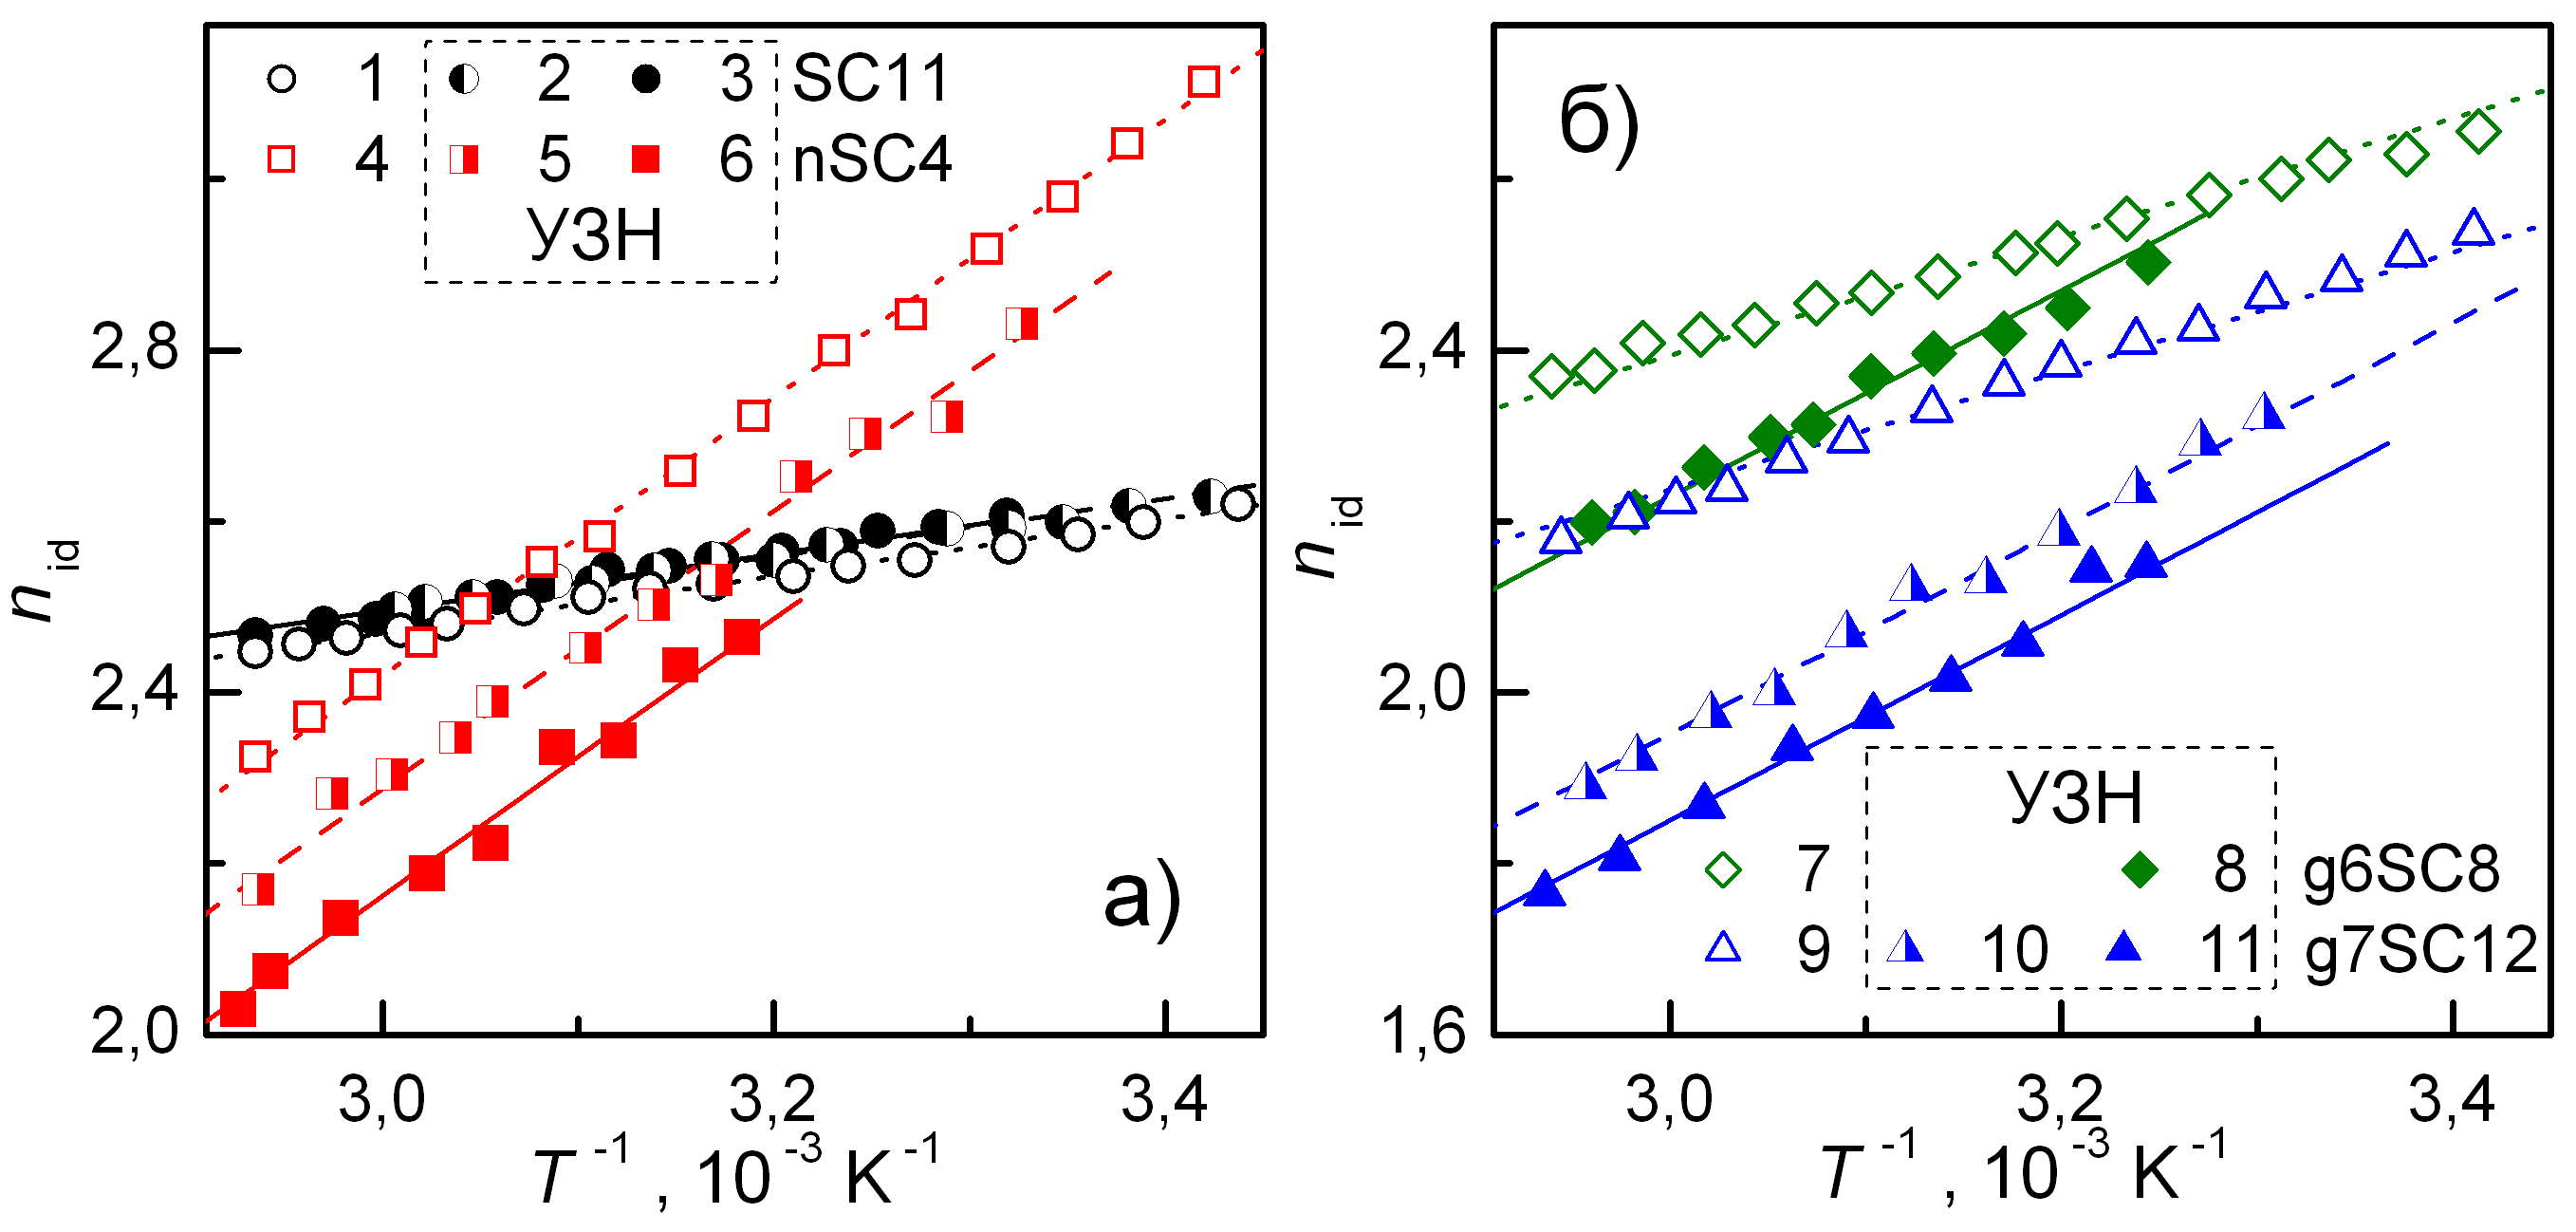
\includegraphics[width=0.95\textwidth]{fignRD}%
\caption{\label{fignRD}
Температурні залежності фактору неідеальності
\FigCaptionSSCRD
Точки --- експеримент,
лінії -- результат апроксимації з використанням формули~(\ref{eq_nT}).
}%
\end{figure}


\begin{figure}
\center
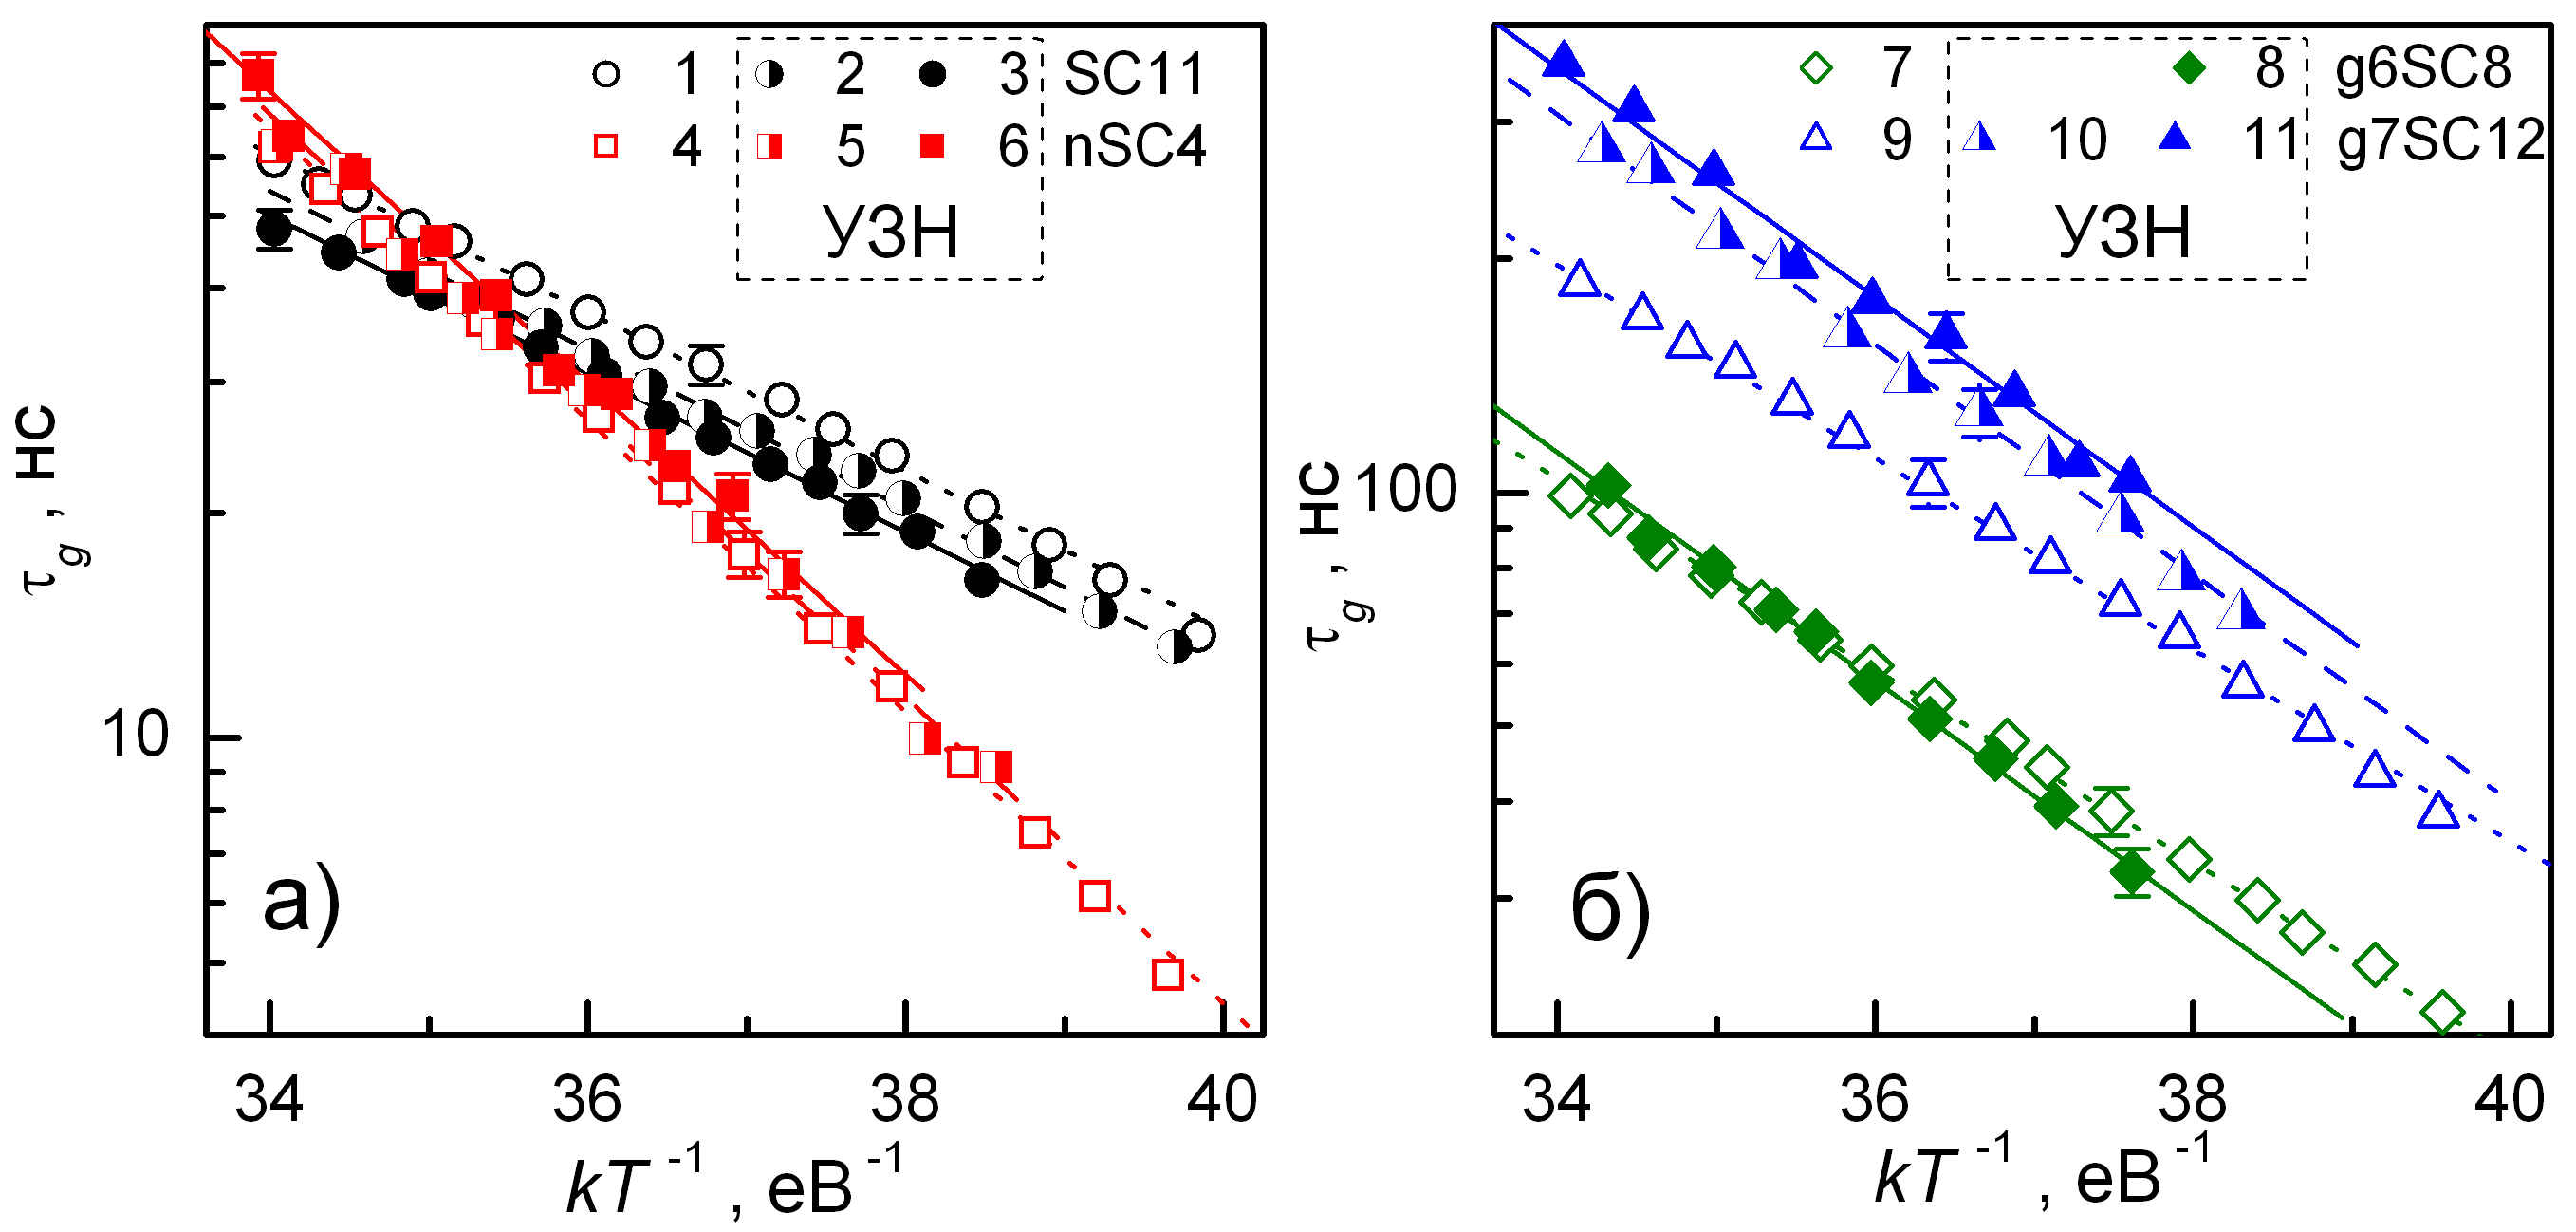
\includegraphics[width=0.95\textwidth]{figTAUgRD}%
\caption{\label{figTAUgRD}
Температурні залежності часу життя в ОПЗ.
Позначення кривих збігаються з Рис.~\ref{fignRD}.
%\FigCaptionSSCRD
Точки --- експеримент,
лінії -- результат апроксимації з використанням формули~(\ref{eq_TAUgT}).
}%
\end{figure}

З рисунків видно, що фактор неідеальності у опромінених структурах зі зменшенням температури зростає,
тоді як для $\tau_{g}$ спостерігається зворотна залежність.
Загалом, зміни $n_{\mathrm{id}}$ та $\tau_{g}$ з температурою добре описуються, як і для неопромінених зразків (див. параграф~\ref{sbQNR}),
 формулами (\ref{eq_nT}) та
(\ref{eq_TAUgT}), відповідно.
Результати відповідної апроксимації також наведені на Рис.~\ref{fignRD} та Fig.~\ref{figTAUgRD},
а визначені значення $T_{\mathrm{id}}$ and $E_{\tau g}$ --- в Таблиці~\ref{tabSSCparRD}.

\begin{table}
\caption{\label{tabSSCparRD}Характеристичні величини температурних залежностей параметрів опромінених та неопромінених
структур $n^+$--$p$--Si.
}
\begin{tabular}{|c|c|c|c|c|c|} \hline
Зразок&УЗН&$T_{\mathrm{id}}$, K&$E_{\tau g}$, еВ&$R_{293,\mathtt{Al}}$, кОм&$\sigma_{\mathtt{dis}}$, $10^4$~K/Ом\\
\hline
SC11&нема&$330\pm30$&$0.24\pm0.01$&$27\pm3$&$41\pm4$\\ \hline
&U--Ts2&$310\pm30$&$0.24\pm0.01$&$27\pm3$&$50\pm4$\\ \hline
&U--Tb3&$360\pm30$&$0.24\pm0.01$&$26\pm3$&$58\pm4$\\ \hline
nSC4&нема&$1610\pm70$&$0.45\pm0.02$&$2.2\pm0.4$&$65\pm7$\\ \hline
&U--Ts3&$1600\pm70$&$0.44\pm0.02$&$2.3\pm0.4$&$95\pm10$\\ \hline
&U--Tb3&$1680\pm70$&$0.44\pm0.02$&$2.2\pm0.4$&$130\pm10$\\ \hline
g6SC8&нема&$610\pm40$&$0.28\pm0.01$&$0.7\pm0.1$&$19\pm2$\\ \hline
&U--Tb2&$1080\pm50$&$0.33\pm0.02$&$0.8\pm0.1$&$24\pm2$\\ \hline
g7SC12&нема&$770\pm50$&$0.29\pm0.01$&$0.41\pm0.06$&$26\pm3$\\ \hline
&U--Ts1&$1260\pm60$&$0.34\pm0.02$&$0.39\pm0.06$&$45\pm4$\\ \hline
&U--Tb1&$1270\pm60$&$0.35\pm0.02$&$0.38\pm0.06$&$55\pm4$\\ \hline
\end{tabular}
\end{table}

При аналізі отриманих результатів, хотілося б наголосити на наступних виявлених особливостях:
\begin{enumerate}[label=\asbuk*),leftmargin=0em,itemindent=1.5em]
\item опромінення викликає зміну величин  $T_{\mathrm{id}}$ та $E_{\tau g}$, причому
 для  g6SC8 характеристична температура фактора неідеальності та характеристична енергія часу життя в ОПЗ
 близькі, за схожих умов, до відповідних значень  g7SC12;

\item в умовах УЗН спостерігається, як і для неопромінених структур, модифікація величин $n_{\mathrm{id}}$ та $\tau_g$;
  величини відповідних змін наведено в Таблиці~\ref{tabAIchangeRD};

\item $\Delta n_{\mathrm{id}}$ та $\varepsilon_{\tau g}$ змінюються при збільшенні $W_{\mathtt{US}}$,
 тоді як $T_{\mathrm{id}}$ та $E_{\tau g}$ практично не залежать від інтенсивності УЗН;

\item УЗН викликає збільшення як  $T_{\mathrm{id}}$, так і $E_{\tau g}$ в $\gamma$--опромінених структурах
(див. Рис.~\ref{fignRD},б та Рис.~\ref{figTAUgRD},б),
тоді як подібний ефект не спостерігається в неопромінених та нейтронно--опромінених зразках
(див. Рис.~\ref{fignRD},а та Рис.~\ref{figTAUgRD},а);

\item АІ зміни фактору неідеальності та часу життя в ОПЗ в опромінених та неопромінених зразках мають протилежний знак
 (для g6SC8 не у всьому температурному діапазоні);

\item зміни фактору неідеальності в умовах УЗН значно більші в радіаційно--модифікованих структурах.
\end{enumerate}


\begin{table}
\caption{\label{tabAIchangeRD}Акусто--індуковані зміни параметрів структур $n^+$-$p$--Si (при 330~K).
}
\center
\begin{tabular}{|c|c|c|c|c|c|} \hline
Зразок&УЗН&$\Delta n_{\mathrm{id}}$, $\pm0.01$&$\varepsilon_{\tau g}$, $\pm5$\%&$\varepsilon_{1/\tau n}$, $\pm0.2$&$\varepsilon_{\sigma\mathtt{dis}}$, $\pm10$\%\\
%&&\mbox{($\pm0.01$)}&($\pm5$\%)&($\pm0.2$)&($\pm10$\%)\\
\hline
SC11&U--Ts2&$-0.02$&14&0.7&$-20$\\
&U--Tb3&$-0.03$&17&1.4&$-40$\\ \hline
nSC4&U--Ts3&0.13&$-5$&1.5&$-50$\\
&U--Tb3&0.26&$-13$&3.0&$-100$\\ \hline
g6SC6&U--Tb2&0.15&$-2$&2.3&$-30$\\ \hline
g7SC12&U--Ts1&0.26&$-49$&0.9&$-70$\\
&U--Tb12&0.36&$-70$&1.9&$-110$\\ \hline
\end{tabular}
\end{table}

Особливості рекомбінації в ОПЗ (великі значення $n_\mathrm{id}$, малі величини та температурна залежність $\tau_g$)
однакові, як  для опромінених структур так і неопромінених.
Тому доцільно припустити, що для nSC4, g6SC8 та g7SC12 процеси в області просторового заряду також можна описати
за допомогою моделі рекомбінації у системі спарених рівнів дефектів, яка детально описана в параграфі~\ref{sbQNR}.
Для пояснені АІ змін параметрів також доцільно залучити модель акусто--активного комплексного дефекту - див. параграф~\ref{sbAEDefect}.
А отже, враховуючи експериментально отримані результати та оцінки, отримані на основі моделі,
\begin{enumerate}[label=\asbuk*),leftmargin=0em,itemindent=1.5em]
\item так як $E_{\tau g}$ (особливо) та $T_{\mathrm{id}}$ (менше) визначаються положенням рівнів, зв'язаних
зі спареними дефектами, то їх зміна в nSC4, g6SC8 та g7SC12 порівняно з SC11 свідчить про те, що
після опромінення змінилися дефекти (або донор, або акцептор, або й обидва), які приймають участь у CDLR;
при цьому за рекомбінацію в g6SC8 та g7SC12 відповідають однакові за типом дефекти (проте з різною концентрацією,
 так як $T_{\mathrm{id}}$ збігаються не абсолютно), які відрізняються від рекомбінаційно активних дефектів в ОПЗ нейтронно--опроміненого зразка;

\item  АІ зміни   $E_{\tau g}$ (та $T_{\mathrm{id}}$), які спостерігаються лише в g6SC8 and g7SC12,
 свідчать про перебудову РД, створених внаслідок $\gamma$--опромінення;
 так як зміни оборотні, то йде мова про те, що відповідні
 гамма--індуковані РД є конфігураційно бістабільними (або метастабільними) і під дією УЗ відбувається їх перебудова з основного стану,
 властивого ненавантаженій внаслідок поширення пружних коливань ґратці;
 подібні АІ перетворення дефектів спостерігалися і раніше \cite{Wosinski,Ostapenko1994,YOlikhTPL2011r};

 \item знак АІ $\varepsilon_{\sigma}$ не міняється (див. Рис.~\ref{figR2L},а та формулу~(\ref{eqEpsSig})), тоді як
  знак  $\varepsilon_{\mathtt{RDA}}$  може мінятися для пари, що складається з дефектів, яким відповідають протилежні
  змінами об'єму кристалу (див. Рис.~\ref{fig_Erda});
  отже зміна знаків $\Delta n_{\mathrm{id}}$ та $\varepsilon_{\tau g}$ свідчить про перехід від випадку
  $(\Delta\Omega_d^\mathtt{D}\cdot\Delta\Omega_d^\mathtt{A}>0)$ до
  $(\Delta\Omega_d^\mathtt{D}\cdot\Delta\Omega_d^\mathtt{A}<0)$ після опромінення;
  на користь такого переходу свідчить і підсилення ефективності впливу УЗН на дефекти в опромінених структурах.
\end{enumerate}

До речі, висновок зроблений в параграфі~\ref{sbDefectType} про те, що
в неопромінених структурах процеси CDLR проходять за участю кисневих преципітатів та комплексу Fe$_i$B$_s$ свідчить на користь
останнього твердження, так як обидва ці дефекти характеризуються $\Delta\Omega_d>0$, тобто є дефектами міжвузольного типу.
Таким чином, в опромінених структурах один з компонентів CDLR--пари
має мати вакансійний тип ($\Delta\Omega_d<0$).

Щодо nSC4, то дефектом, який здатен пояснити АІ зміни $\tau_g$ та $n_\mathrm{id}$, цілком може бути дивакансія,
значна кількість яких утворюється при нейтронному опроміненні.
Проте у гамма--опромінених зразках очікується поява бістабільного (або метастабільного) дефекту.
Загалом у кремнії відомо лише декілька подібних дефектів з $\Delta\Omega_d<0$, а саме
\begin{itemize}
  \item VO$_2$ \cite{FTP:Murin},
  \item V$_3$ \cite{V3:Markevich},
  \item VO$_i$ \cite{MetaUFN}.
\end{itemize}
Проте комплекс VO$_2$ утворюється в радіаційно--опромінених кристалах після відпали при $300^\circ$C,
V$_3$ не є типовим дефектом для кремнію, опроміненого $\gamma-^{60}$Co,
тоді як VO$_i$ при цьому утворюються у достатній кількості (див. Таблицю~\ref{tabDefectNt}) і можуть приймати
участь в CDLR в околі $n^+$--$p$ інтерфейсу в g6SC8 and g7SC12.
Метастабільний стан VO$_i$ зазвичай спостерігається при низьких температурах
і відрізняється більшою відстанню між вакансією та киснем та глибшим розташуванням енергетичного рівня \cite{MetaUFN}.
Для комплексу як цілого $\Delta\Omega_d(\mbox{VO}_i)<0$,
проте для його компонент $\Delta\Omega_d(\mbox{V})<0$ та $\Delta\Omega_d(\mbox{O}_i)>0$.
Таким чином, згідно зі зробленими при розгляді акусто--активного комплексу припущеннями,
VO$_i$ є цілком придатним для АІ зміни відстані між компонентами.
Отримані результати свідчать, що під дією УЗН  відбувається
перехід VO$_i$ у метастабільну конфігурацію, що, в свою чергу,
викликає зміни $T_{\mathrm{id}}$ та $E_{\tau g}$.





\subsection{Квазі--нейтральна область\label{sbRadDef}}

Чисельним показником рекомбінаційних процесів, які відбуваються в КНО $p$-$n$ структури є
час життя неосновних носіїв заряду.
Рис.~\ref{figTAUrRD} відображає виявлену поведінку $\tau_n$ зі зміною температури як для опромінених зразків,
так і неопромінених, як при застосуванні УЗН, так і без нього.
Загалом, залежності $\tau_n$ від температури та УЗН не змінюються після радіаційного впливу.
Вихідні значення $\tau_n$ знаходяться в діапазоні $2\div5$~мкс для різних зразків,
що відповідає довжинам дифузії $80\div130$~мкм.
При опроміненні використовувалися не дуже високі дози і тому
такий розкид значень часів життя не зв'язаний саме з радіаційним впливом,
а швидше визначається неоднорідністю вихідної пластини, з якої були виготовлені зразки.
Подібна неоднорідність зустрічається досить часто \cite{Oxide:Chen,Oxide_Schon}.


\begin{figure}
\center
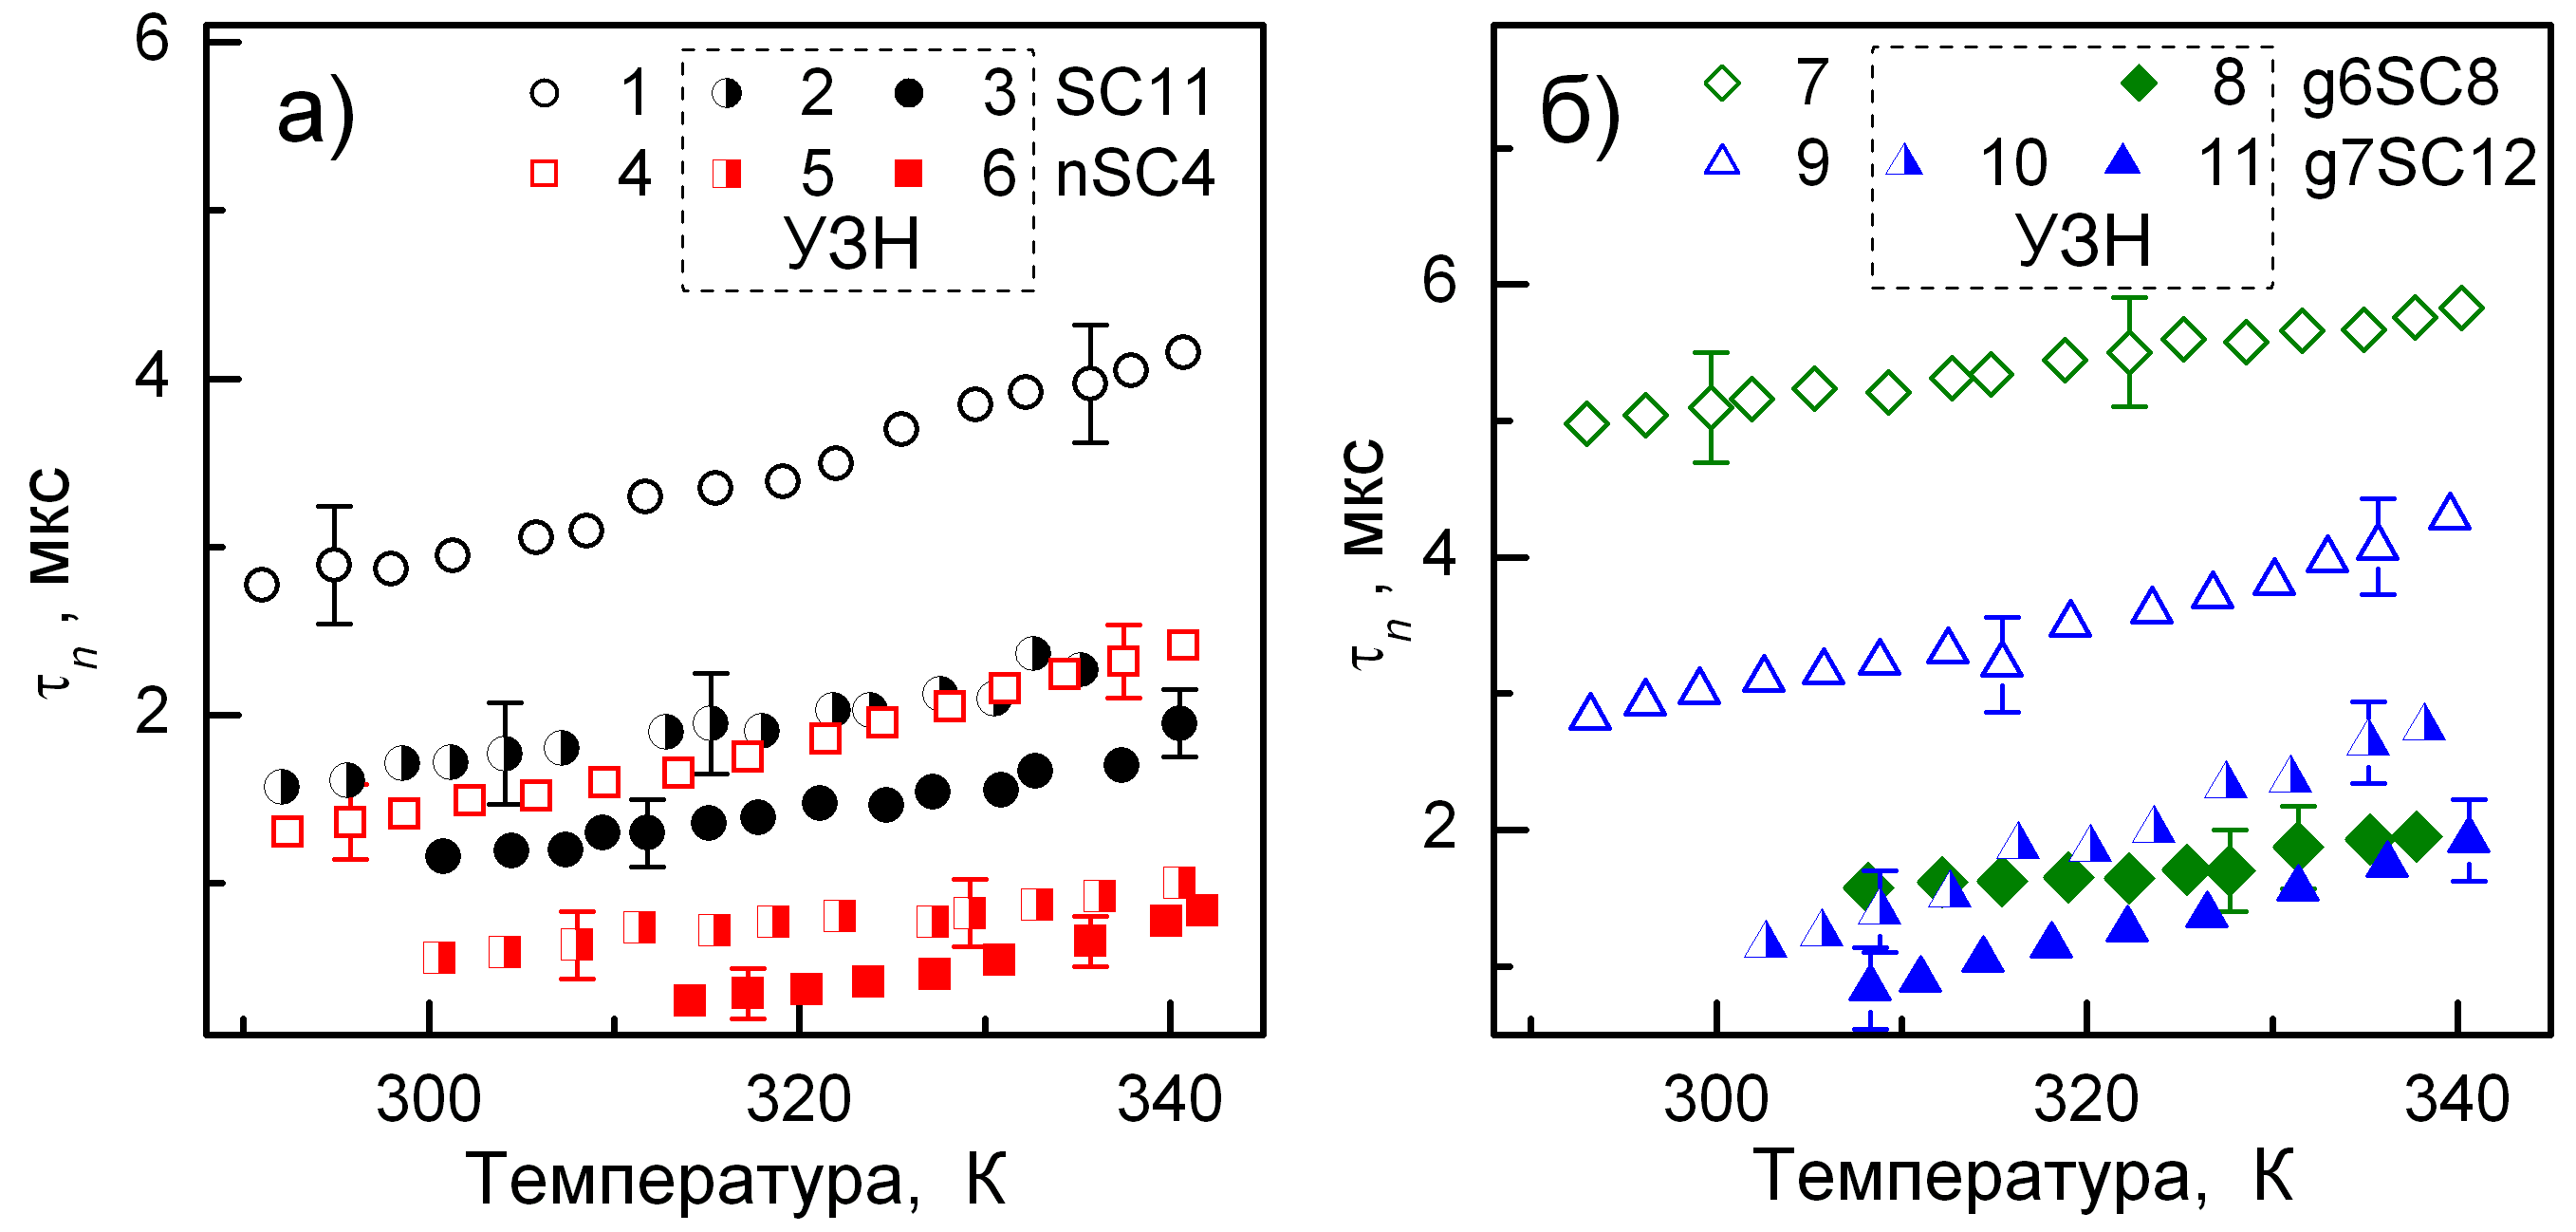
\includegraphics[width=0.95\textwidth]{figTAUrRD}
\caption{\label{figTAUrRD}
Температурні залежності часу життя неосновних носіїв заряду в КНО
\FigCaptionSSCRD
%. Позначення кривих збігаються з Рис.~\ref{fignRD}.
}%
\end{figure}

З іншого боку, для опису радіаційно--індукованого зменшення часу життя використовується формула Messenger–-Spratt \cite{Markvart}:
\begin{equation}
\label{eqMS}
\tau_n^{-1}=\tau_{n0}^{-1}+K_\tau\Psi\,,
\end{equation}
де
$\tau_{n0}$ відповідає неопроміненому зразку, а
$K_\tau$ --- константа пошкодження часу життя (lifetime damage constant).
Загалом $K_\tau$ залежить від кристалу, типу опромінення і насамперед визначається величиною NIEL.
Відомі з літератури значення $K_\tau$ для Cz--Si та проведені з використанням виразу (\ref{eqMS}) оцінки відповідних
змін оберненого часу життя наведено в Таблиці~\ref{tabTAUn}.
Як видно з наведених даних, оцінені значення радіаційно--індукованих змін $\tau_n^{-1}$ складають лише
(8-17), 4 та 29\% виміряних значень для зразків nSC4, g6SC8 та g7SC12, відповідно, а отже не можуть
пояснити екпериментально виявлений розкид даного параметру.

\begin{table}
\caption{\label{tabTAUn}Виміряні та оцінені параметри часу життя в КНО.
}
\center
\begin{tabular}{|c|c|c|c|c|}
\hline
Зразок &$\tau_{n,in}^{-1}$ (320~K), 10$^5$~с$^{-1}$&$K_\tau$, см$^2/$с&$K_\tau\times\Psi$, 10$^4$~с$^{-1}$&$K_\mathtt{US}^\mathtt{eff}$, см$^2/$Вт\\ \hline
SC11&2,9&$\ldots$&$\ldots$&3,5\\ \hline
\multirow{2}{*}{nSC4}&\multirow{2}{*}{4,7}&10$^{-7}$ \cite{NIEL:Jafari}&\multirow{2}{*}{4$\div$8}&\multirow{2}{*}{7,1}\\ %\hline
&&2$\times$10$^{-7}$ \cite{n:Gaubas}&&\\ \hline
g6SC8&1,8&5$\times$10$^{-12}$&0,8&6,0\\ \cline{1-2} \cline{4-5}%\hline
g7SC12&2,8& \cite{NIEL:Jafari,gamma:Kolkov} &8&5,2\\ \hline
\end{tabular}
\end{table}

З іншого боку,
оцінка впливу утворених РД на час життя неосновних носіїв заряду в КНО може бути проведена спираючись
на вираз (\ref{eqTAUSHRsum}).
При цьому необхідно взяти до уваги,
що VO$_i$ не є рекомбінаційно--активним центром у $p$--Si \cite{gamma:Kolkov,IrrCzpSi:Benton,IrrCzpSi:Coffa,IrrCzpSi:Ganagona,IrrCzpSi:Vines}.
Була проведена оцінка величин $\tau_{n,\mathtt{RD}}^{-1}$ (оберненого часу життя, пов'язаного з рекомбінацією на окремих РД)
для C$_i$O$_i$, V$_2$ та  V$_3$, спираючись на їх концентрацію (див. Таблицю~\ref{tabDefectNt}) та відомі з літератури значення ППЗ електронів.
Отримані результати наведено в Таблиці~\ref{tabDefectTAU}.
Видно, що на $\tau_n$ в гамма--опромінених зразках переважно впливають комплекси C$_i$O$_i$, тоді як для nSC4 основні очікувані
зміни часу життя пов'язані з вакансійними кластерами.
Зауважимо, що для nSC4, g6SC8 та g7SC12 сума величин $\tau_{n,\mathtt{RD}}^{-1}$ для різних дефектів
непогано збігається з відповідними значеннями $(K_\tau\cdot\Psi)$ (Таблиця~\ref{tabTAUn})




\begin{table}[b]
\caption{\label{tabDefectTAU}Оцінка впливу окремих РД на час життя неосновних носіїв в КНО.
}
\center
\begin{tabular}{|c|c|c|c|c|}
\hline
Дефект&$\sigma_n$,&\multicolumn{3}{c|}{$\tau_{n,\mathtt{RD}}^{-1}$, 10$^4$~с$^{-1}$}\\ \cline{3-5}
&10$^{-15}$~см$^2$&nSC&g6SC&g7SC\\
\hline
C$_i$O$_i$&0,7 \cite{gamma:Stahl}, 0,9 \cite{gamma:Kolkr}&0,8--1&0,9--1,1&9--11\\ \hline
V$_2$&3 \cite{gamma:Stahl}, 2 \cite{A:Brothe}&2,2--3,3&0,1--0,2&1--2\\ \hline
V$_3$&2,4 \cite{V3:Markevich}&0,7&---&---\\ \hline
\end{tabular}
\end{table}

Рис.~\ref{figTAUrRD} показує, що УЗН викликає зменшення $\tau_n$.
З виразу (\ref{eqTAUSHRsum}) видно, що при аналізі змін $\tau_n$
зручніше розглядати відносні зміни оберненого часу життя
\begin{equation*}
  \varepsilon_{1/\tau n}=\frac{\tau_{n,\mathtt{US}}^{-1}-\tau_{n,in}^{-1}}{\tau_{n,in}^{-1}}=\frac{\tau_{n,in}-\tau_{n,\mathtt{US}}}{\tau_{n,\mathtt{US}}}\,.
\end{equation*}
АІ значення наведено в Таблиці~\ref{tabAIchangeRD}.

Використовуючи модель акусто--активного комплексу (параграф~\ref{sbAEDefect}, формули (\ref{eqEpsSigUS}) та (\ref{eqEpsSigUSA}))
вираз для $\varepsilon_{\tau n}$ можна перетворити наступним чином
\begin{equation}
\label{eqEpsTAU}
\varepsilon_{1/\tau n}=K_\mathtt{US}^\mathtt{eff}W_\mathtt{US}\,,
\end{equation}
де
$K_\mathtt{US}^\mathtt{eff}$ характеризує АДВ у зразку і залежить від
концетрацій як ААД, так і не акусто--активних (non--AA) центрів
\begin{equation}
\label{eqKeff}
K_\mathtt{US}^\mathtt{eff}=\sum_j^{M_d^\mathtt{AA}}\frac{\tau_{n,in}}{\tau_{n,j,in}}K_\mathtt{US,j}^{*}\,.
\end{equation}
Як вже було зазначено, $K_\mathtt{US,j}^*$ описує взаємодію $j$--го рекомбінаційного центру з ультразвуком.
Отримані залежності $\varepsilon_{1/\tau n}$ від $W_\mathtt{US}$ показано на Рис.~\ref{figKusRD}.
Лінійність цих залежностей ще раз підтверджує справедливість припущень, використаних при побудові
моделі.
Визначені величини $K_\mathtt{US}^\mathtt{eff}$ наведено в Таблиці~\ref{tabTAUn}.


\begin{figure}
\center
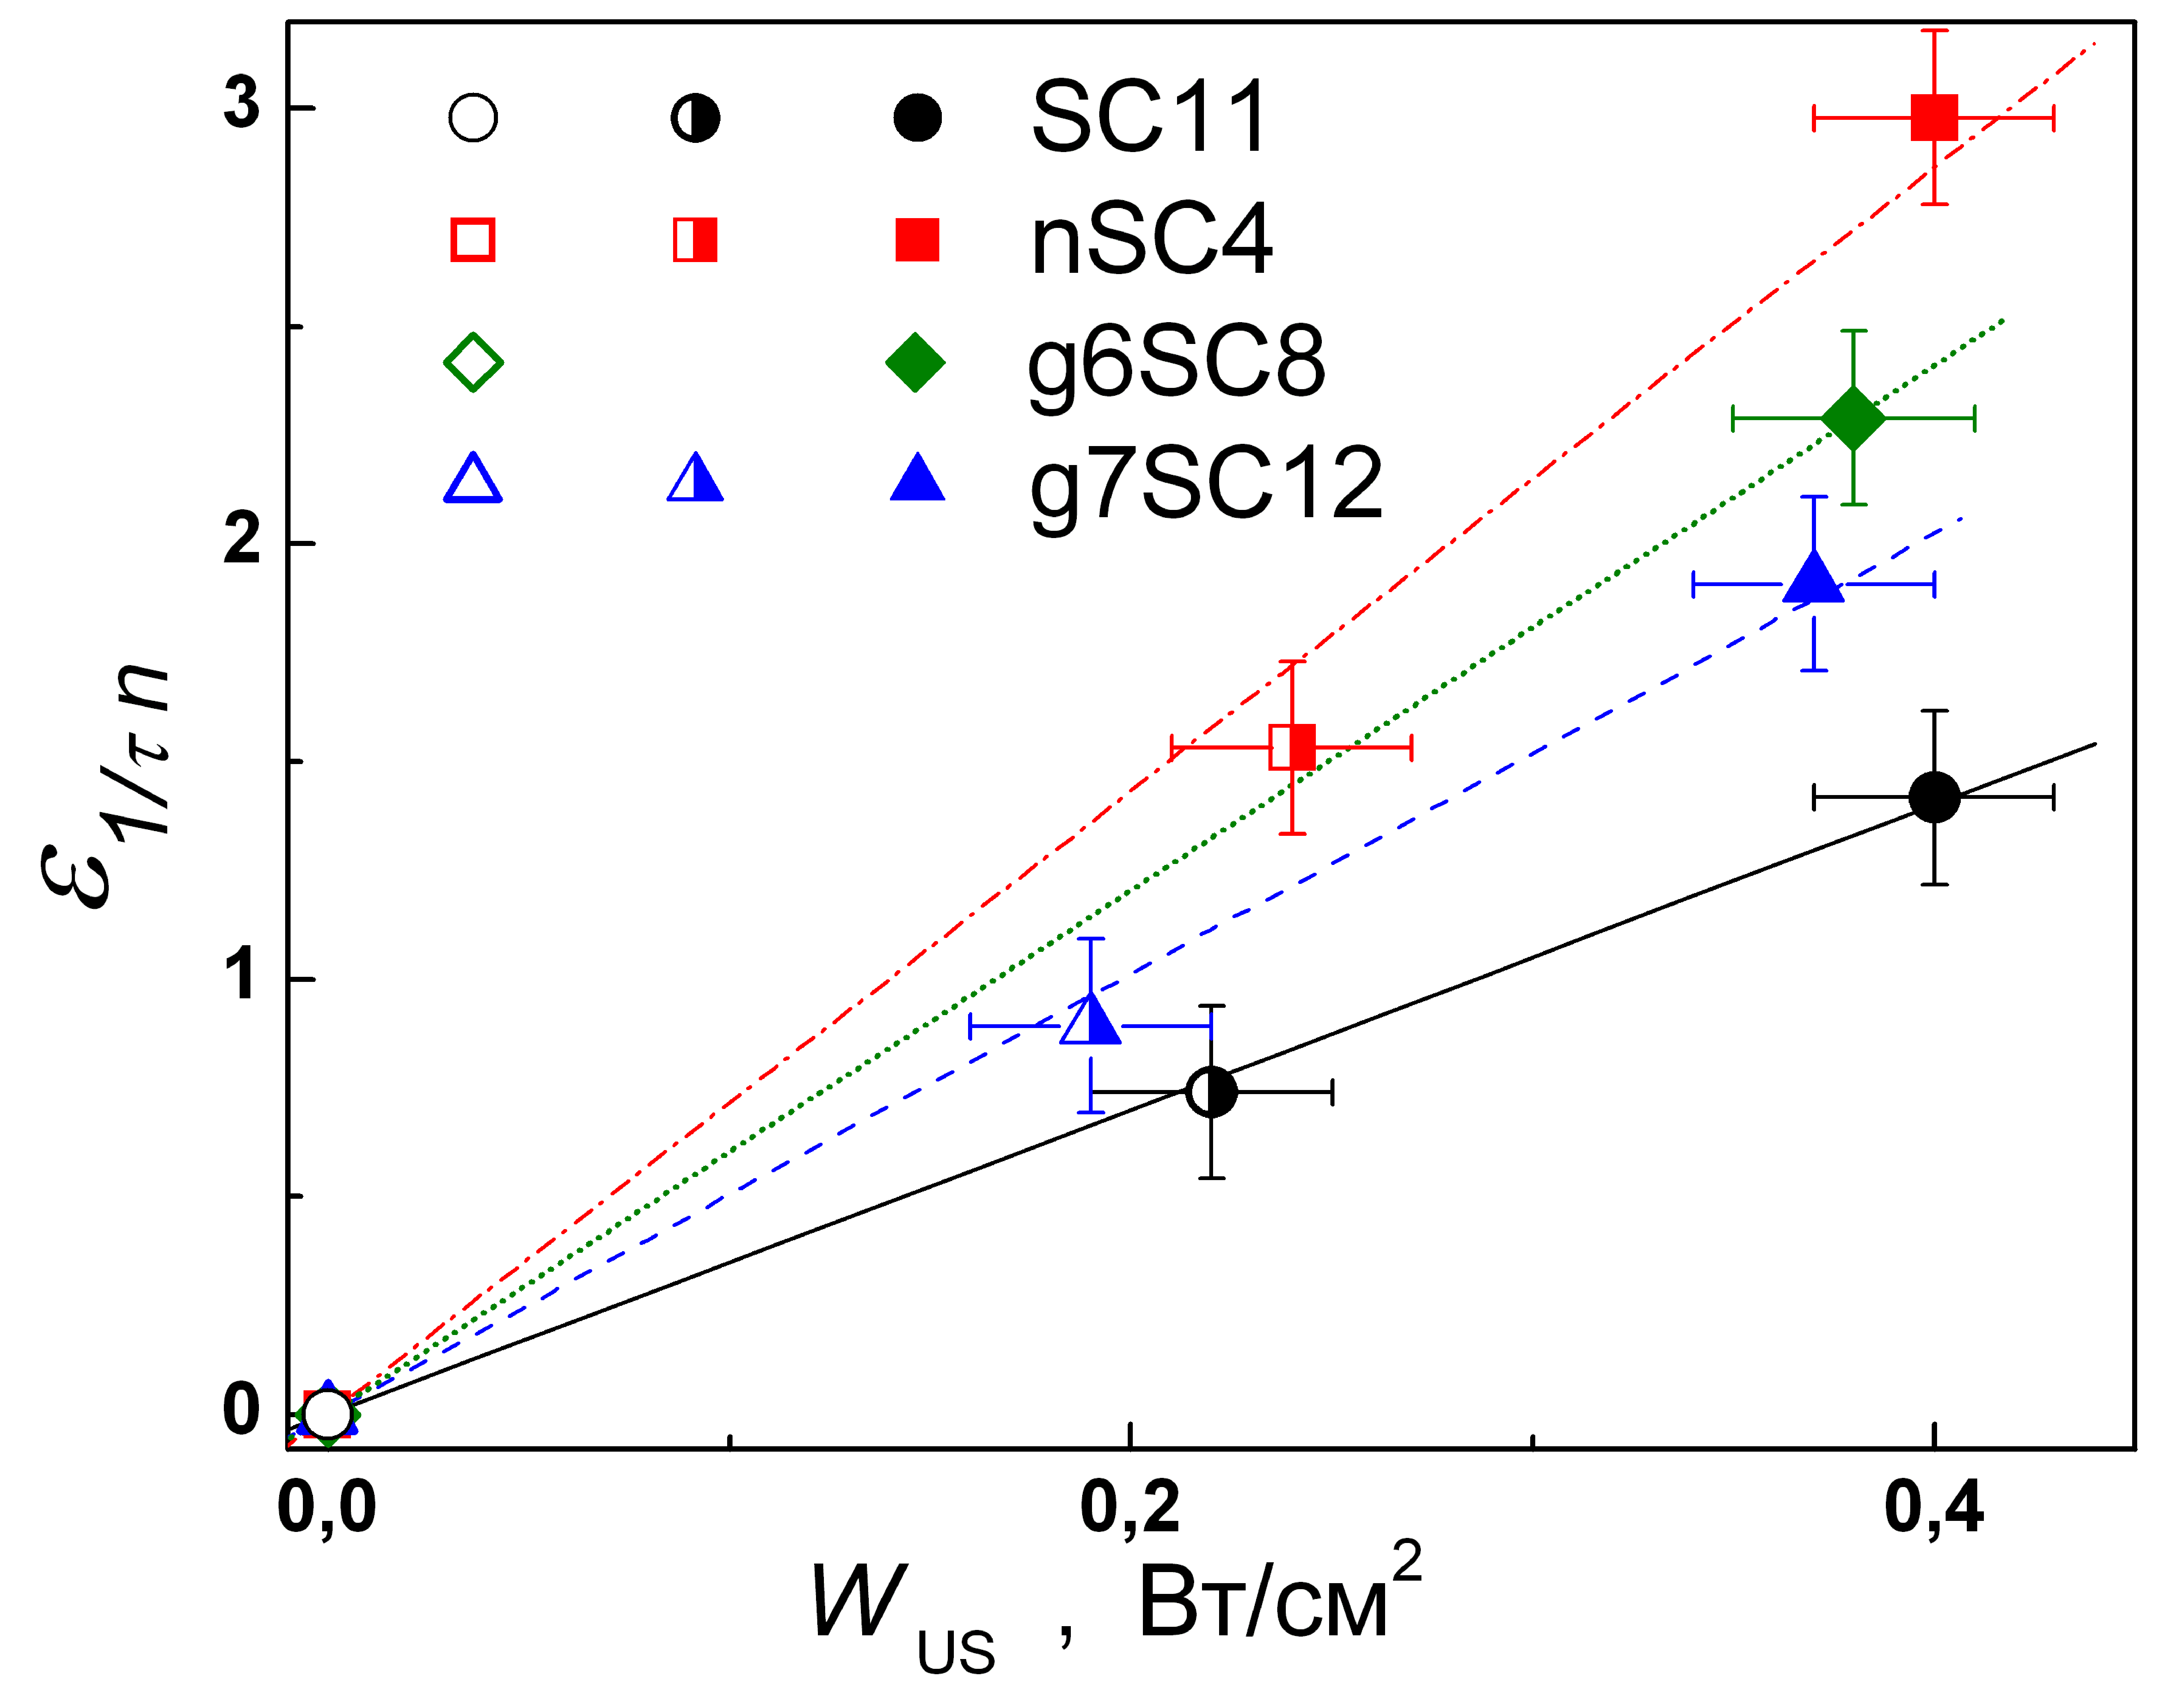
\includegraphics[width=0.65\textwidth]{figKusRD}
\caption{\label{figKusRD}
Залежності відносних змін оберненого часу життя в ОПЗ від інтенсивності УЗ для
неопроміненого (кола), нейтронно--опроміненого (квадрати) та $\gamma$--опромінених (трикутники та ромби) зразків.
Лінії --- апроксимація згідно з формулою ~(\ref{eqEpsTAU}).
}%
\end{figure}

Припустимо,
що в неопромінених зразках присутні ААД лише одного типу, тобто $M_d^\mathtt{AA}=1$.
Відповідно до результатів, наведених в параграфі~\ref{sbDefectType}, це можуть бути дефекти, пов'язані з кисневмісними преципітатами.
Позначимо константи взаємодії УЗ із C$_i$O$_i$ та V$_n$ як $K_\mathtt{US}^\mathtt{CO}$ та $K_\mathtt{US}^\mathtt{V}$, відповідно.
В цьому випадку вираз для $K_\mathtt{US}^\mathtt{eff}$ в неопромінених та опромінених зразках
матиме вигляд (\ref{eqeqKeffInit}) та (\ref{eqeqKeffRD}), відповідно:
\begin{eqnarray}
K_\mathtt{US}^\mathtt{eff}&=&K_\mathtt{US}^\mathtt{AA}\,\tau_{n,in}/\tau_{n,in}^\mathtt{AA}\,,\label{eqeqKeffInit}\\
K_\mathtt{US}^\mathtt{eff}&=&K_\mathtt{US}^\mathtt{AA}\tau_{n,in}/\tau_{n,in}^\mathtt{AA}+
                           K_\mathtt{US}^\mathtt{CO}\tau_{n,in}/\tau_{n,\mathtt{RD}}^\mathtt{CO}+
                           K_\mathtt{US}^\mathtt{V}\tau_{n,in}/\tau_{n,\mathtt{RD}}^\mathtt{V} \,.\label{eqeqKeffRD}
\end{eqnarray}
У цих виразах $\tau_{n,in}^\mathtt{AA}$ --- час життя неосновних носіїв за умови, що рекомбінація
відбувається лише за участю ААД (non--AA рекомбінаційні центри відсутні),
а $K_\mathtt{US}^\mathtt{AA}$ описує АДВ з цим дефектом.

Для аналізу найбільш придатні два граничні випадки.
В першому з них вважається,
що ААД розподілені однорідно по кремнієвій пластині, тоді як
non--AA рекомбінаційні центри --- неоднорідно.
Іншими словами,
значення $\tau_{n,in}^\mathtt{AA}$ для зразків SC11, nSC4, g6SC8 та g7SC12
однакове, тоді як різниця величин
$(\tau_{n,in}^{-1}-K_\tau\cdot\Psi)$ визначається non--AA дефектами.
Використовуючи вирази (\ref{eqeqKeffInit}) та (\ref{eqeqKeffRD}) а також
дані таблиць \ref{tabTAUn} та \ref{tabDefectTAU}
була отримана наступна система рівнянь
\begin{eqnarray}
\mbox{SC11}:\,\,3.5&=&K_\mathtt{US}^\mathtt{AA}\cdot(\tau_{n,in}^\mathtt{AA})^{-1}\,/2.9\,,\nonumber\\
\mbox{nSC4}:\,\,7.1&=&K_\mathtt{US}^\mathtt{AA}\cdot(\tau_{n,in}^\mathtt{AA})^{-1}\,/4.7+0.09\,K_\mathtt{US}^\mathtt{V}+0.02\,K_\mathtt{US}^\mathtt{CO}\,,\nonumber\\
\mbox{g6SC8}:\,\,6.0&=&K_\mathtt{US}^\mathtt{AA}\cdot(\tau_{n,in}^\mathtt{AA})^{-1}\,/1.8+0.01\,K_\mathtt{US}^\mathtt{V}+0.05\,K_\mathtt{US}^\mathtt{CO}\,,\nonumber\\
\mbox{g7SC12}:\,\,5.2&=&K_\mathtt{US}^\mathtt{AA}\cdot(\tau_{n,in}^\mathtt{AA})^{-1}\,/2.8+0.05\,K_\mathtt{US}^\mathtt{V}+0.35\,K_\mathtt{US}^\mathtt{CO}\,,\nonumber
\end{eqnarray}
де
$(\tau_{n,in}^\mathtt{AA})^{-1}$ вимірюється в $10^4$~с$^{-1}$.
Ці рівняння є справедливими за умови, що
$K_\mathtt{US}^\mathtt{AA}\cdot(\tau_{n,in}^\mathtt{AA})^{-1}=(10\pm3)$~см$^2$~Вт$^{-1}$,
$K_\mathtt{US}^\mathtt{V}=(42\pm15)$~см$^2$~Вт$^{-1}$,
$K_\mathtt{US}^\mathtt{CO}=0$.
Так як  $(\tau_{n,in}^\mathtt{AA})^{-1}<1,83$,
то $K_\mathtt{US}^\mathtt{AA}>5$~см$^2$~Вт$^{-1}$.

У іншому граничному випадку вважається,
що non--AA розподілені по пластині рівномірно,
тоді як ААД визначають відмінність значень $(\tau_{n,in}^{-1}-K_\tau\cdot\Psi)$ у різних зразках.
Проте, якщо записати систему рівнянь, використовуючи дані припущення,
то виявляється що експериментально визначені значення $K_\mathtt{US}^\mathtt{eff}$
приводять до фізично неправильних (від'ємних) значень $K_\mathtt{US,j}^*$.
Подібні нереальні результати отримуються і у припущені, що $M_d^\mathtt{nonAA}=0$
(non--AA рекомбінаційні центри відсутні).

Таким чином, отримані результати дозволяють зробити висновок,
що лише частина дефектів, пов'язаних з КП, є акусто--активними.
Вони розподілені достатньо рівномірно по вихідній кремнієвій пластині і саме їх модифікація
в умовах УЗН є причиною виявлених зміни часу життя неосновних носіїв заряду в неопромінених та $\gamma$--опромінених зразках.
Ефект АІ зміни $\tau_n$ підсилюється внаслідок АІ модифікації дивакансій у нейтронно--опромінених структурах.
Іншими словами,
C$_i$O$_i$ не є акусто--активним дефектом, тоді як V$_2$ має подібні властивості.



\subsection{Акусто--індуковані зміни шунтуючого опору\label{sbRsh}}

На Рис.~\ref{figRshRD} наведено залежність величини шунтуючого опору опромінених та неопромінених структур
за умов УЗН та без нього для дослідженого температурного інтервалу.
Як видно з рисунку, опромінення викликає достатньо суттєве зниження шунтуючого опору, а отже
і збільшення шунтуючого струму.
Крім того, після $\gamma$--опромінення відбувається зміна температурної залежності $R_{sh}$:
так, якщо для SC11 та nSC4 спостерігається зменшення шунтуючого опору з ростом температури,
то для g6SC8 та g7SC12 в околі 293~K спостерігається майже лінійне збільшення залежності
$R_{sh}$ від $T$.
Зауважимо, що вісь $R_{sh}$ на Рис.~\ref{figRshRD},a має логарифмічний масштаб і лінійний на  Рис.~\ref{figRshRD},б.


\begin{figure}
\center
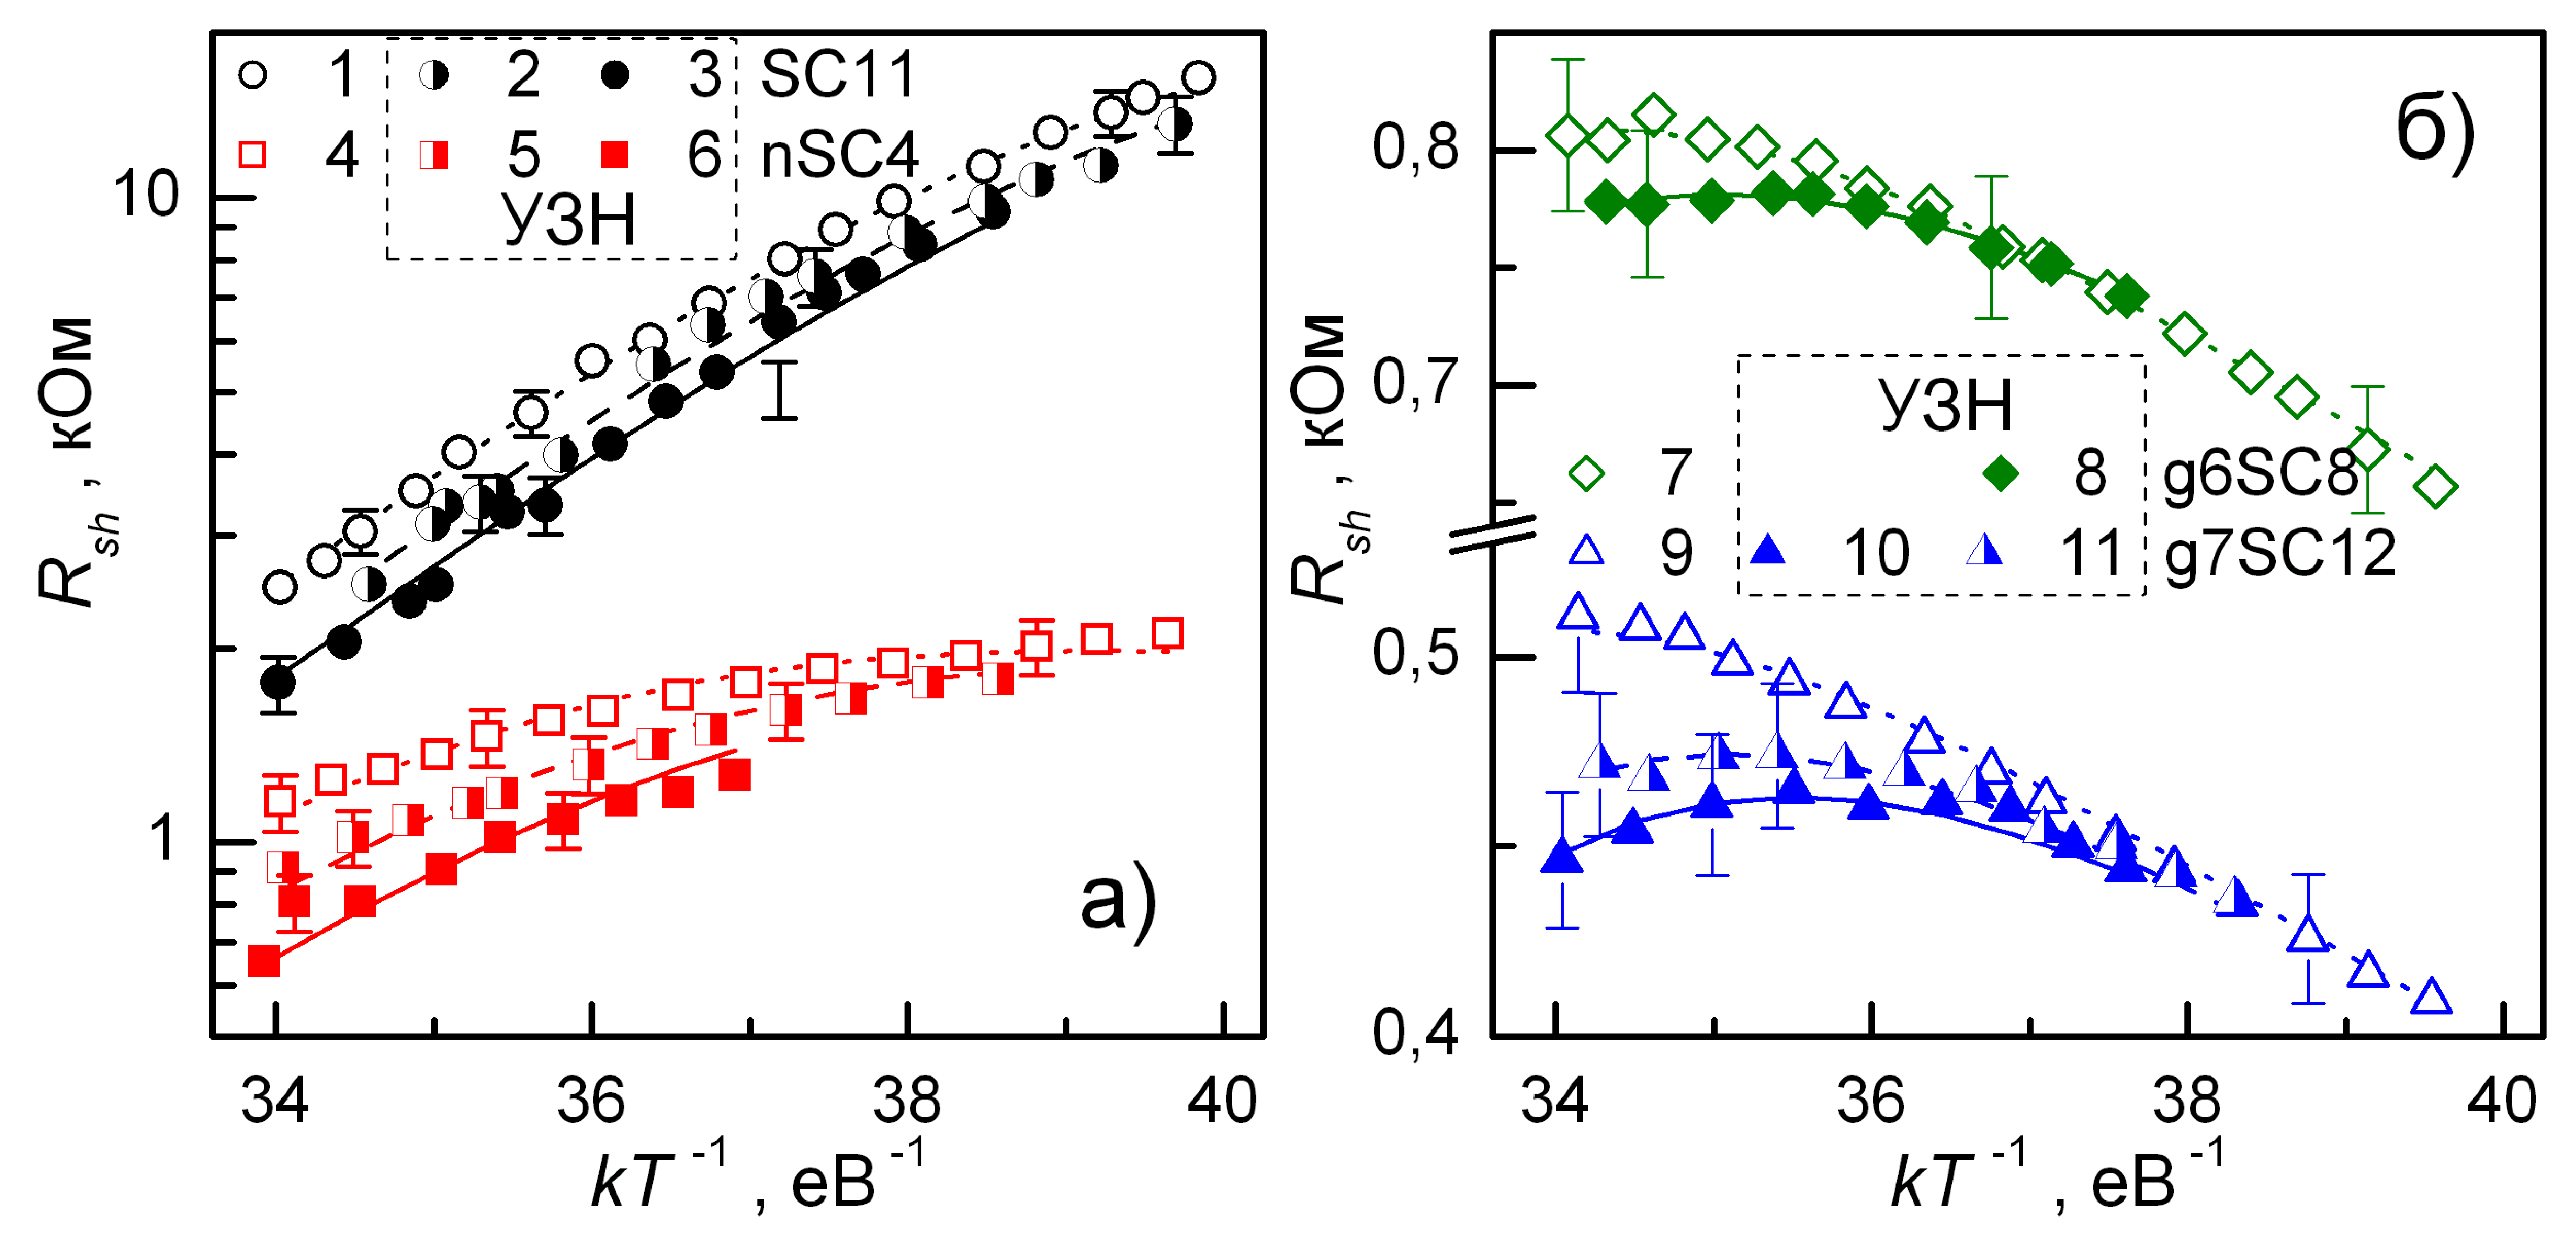
\includegraphics[width=1.0\textwidth]{figRshRD}
\caption{\label{figRshRD}
Температурні залежності величини шунтуючого опору
\FigCaptionSSCRD
%Позначення кривих збігаються з Рис.~\ref{fignRD}.
Точки --- експеримент,
лінії -- результат апроксимації з використанням формул~(\ref{eqRshFull})-(\ref{eqRsh}).
}%
\end{figure}

Відомо \cite{Rsh:Breitenstein,RshMet,Breitenstein2013}, що для появи шунтуючого опору в $p$--$n$ структурах існує декілька причин, не
пов'язаних з механічним ушкодженням.
Так, причиною його появи можуть бути часточки алюмінію, макроскопічні включення Si$_3$N$_4$, кристалічні волокна SiC або утворення інверсійних шарів
в околі преципітатів.
Проте три  останні утворення зустрічаються переважно у мультикристалічних КСЕ \cite{Rsh:Breitenstein,Breitenstein2013} і не можуть
бути причиною шунтуючого опору для досліджених кристалічних зразках.
В той же час вважається, що під час відпалу, необхідного для утворення контактів, частинки Al проникають у зразок,
створюючи навколо себе області з високою концентрацією дірок ($p^+$).
Наявність таких компенсованих областей в емітері КСЕ  забезпечує омічний контакт з базою.

Крім того, в літературі показано \cite{Rsh:Breitenstein,TAT:Gopal,Rsh:Baker,Si:dislIV},
що дислокації, які перетинають область $p$--$n$ переходу, теж можуть бути причиною появи омічного струму.
Наприклад, наявність навіть декількох дислокації в діодних кремнієвих структурах викликає зменшення питомого опору
та зміну форми ВАХ, характерну для підвищення ролі шунтуючого опору \cite{Si:dislIV}.
В досліджених структурах причиною появи дислокацій можуть бути кисневмісні преципітати, при утворенні яких
виникають лінійні дефекти \cite{SiO:Hwang,SiO:Vanhell}, а також напруги, що виникають
на границі сильнолегованої $n$--області та слабколегованої бази.

На нашу думку, в досліджених структурах присутні і дислокації, і частки алюмінію.
В цьому випадку повний шунтуючий опір може бути записаний у вигляді
\begin{equation}
\label{eqRshFull}
R_{sh}^{-1}=R_{sh,\mathtt{Al}}^{-1}+R_{sh,\mathtt{dis}}^{-1}\,,
\end{equation}
де
$R_{sh,\mathtt{Al}}$ та $R_{sh,\mathtt{dis}}$ відображають внески часток алюмінію та дислокацій, відповідно.
Для опору металеву частинки очікується лінійна температурна залежність:
\begin{equation}
\label{eqRshAl}
R_{sh,\mathtt{Al}}=R_{293,\mathtt{Al}}[1+\alpha_R(T-293)]\,,
\end{equation}
де
$R_{293,\mathtt{Al}}$ --- величина шунтуючого опору при 293~K,
а
$\alpha_R$ --- температурний коефіцієнт опору.

З іншого боку, відповідно до моделі дислокаційно--індукованого імпедансу фотовольтаїчних детекторів,
запропонованої в роботах \cite{Rsh:Gopal2003,Rsh:Gopal2004},
$R_{sh,\mathtt{dis}}$ може бути записаний у вигляді:
\begin{equation}
\label{eqRsh}
R_{sh,\mathtt{dis}}=\frac{T}{\sigma_{\mathtt{dis}}}\left[\cosh\left(\frac{E_\mathtt{dis}-E_i}{kT}\right)+\cosh\left(\frac{U_s}{kT}\right)\right]\,,
\end{equation}
де
\begin{equation}
\label{eqRdis}
\sigma_{\mathtt{dis}}=\rho_{\mathtt{dis}}Aq^2A_{\mathtt{dis}}\sqrt{K_nK_p}\,N_{\mathtt{dis}}(n_p+p_p)/k\,,
\end{equation}
$E_{\mathtt{dis}}$ --- енергетичне положення рівня, що відповідає за появу
дислокаційного рекомбінаційного струму;
$U_s$ --- потенціал на поверхні дислокаційного ядра,
$\rho_{\mathtt{dis}}$ та $A_{\mathtt{dis}}$ --- густина та площа поверхні дислокацій,
$K_n$ та $K_p$ --- ймовірності захоплення електронів та дірок дислокаційними станами,
are the probabilities for electrons and holes capture by the dislocation states,
$N_{\mathtt{dis}}$ --- густина поверхневих станів на кожній дислокації.
Вираз~(\ref{eqRsh}) записано для спрощеного випадку $K_p=K_n$.

В роботі температурний коефіцієнт опору був оцінений за даними для зразка g7SC12 в околі кімнатної температури.
Отримана величина $8,3\cdot10^{-3}$~K$^{-1}$ не дуже суттєво відрізняється від температурного
коефіцієнту опору об'ємного алюмінію ($4,3\cdot10^{-3}$~K$^{-1}$),
що підтверджує доцільність зроблених припущень.
Надалі, використовуючи отримане значення $\alpha_R$, була
проведена апроксимація температурних залежностей $R_{sh}$ відповідно до формул (\ref{eqRshFull})--(\ref{eqRsh}).
При цьому шуканими параметрами вважалися $R_{293,\mathtt{Al}}$, $(E_{\mathtt{dis}}-E_i)$, $U_s$ та $\sigma_{\mathtt{dis}}$.
Виявилось, що експериментальні залежності добре описуються апроксимуючими кривими (див. Рис.~\ref{figRshRD})
при значеннях $(E_{\mathtt{dis}}-E_i)=(0.46\pm0.02)$~еВ та $U_s=(5\pm4)\times10^{-8}$~еВ,
причому ці величини не залежать від опромінення та УЗН.
Отримана величина $(E_{\mathtt{dis}}-E_i)$ відповідає енергії активації носіїв $0.10\pm0.02$~еВ.
Це, в свою чергу, досить близько до енергії активації дислокаційних рівнів $0.08$~еВ,
яка спостерігалася раніше \cite{disl10:Castaldini,disl10:Isakova,disl10:Yur,disl10:Kveder,disl10:Trushin,Si:disl},
у тому числі і в Cz--Si:B \cite{disl10:Castaldini,disl10:Isakova,disl10:Yu}.
Зауважимо, що дислокаціям в напівпровідникових кристалах відповідають як мілкі,
так і глибокі рівні \cite{Disl:GaN};
якщо в параграфі~\ref{sBulyrMethod} акцент було зроблено на глибокі, то на шунтуючий опір, як виявилося,
переважний вплив мають мілкі.


Отримані значення $R_{293,\mathtt{Al}}$ та $\sigma_{\mathtt{dis}}$ наведено в Таблиці~\ref{tabSSCparRD}.
$R_{293,\mathtt{Al}}$ не залежить від УЗН та зростає з опроміненням.
На нашу думку, виявлена зміна характеру температурної залежності шунтуючого опору пояснюється
наступним чином.
Для неопромінених зразків $R_{sh,\mathtt{dis}}$ менший ніж $R_{sh,\mathtt{Al}}$ і шунтуючий опір
у структурі визначається насамперед рекомбінацією на дислокаціях, які перетинають площину $p-n$ переходу,
утворюючи канали для проходження носіїв заряду.
При опроміненні утворюються вакансії, що полегшує дифузію атомів Al з електродів, насамперед з фронтального у емітер.
В результаті кількість часточок Al та їх розмір зростає, $R_{sh,\mathtt{Al}}$ зменшується,
перетворюючись при високих дозах на ключовий фактор визначення повного шунтуючого опору.
Дифузія Al у $\gamma$--опромінених зразках відбувається більш ефективно через те, що
 при такому способі впливу утворюються окремі рівномірно розподілені по об'єму вакансії, тоді
 як при нейтронному опроміненні виникають рідко розташовані вакансійні кластери.
Як наслідок, в nSC4 величина $R_{sh,\mathtt{Al}}$ хоч і зменшується, проте залишається
більшою ніж дислокаційно--індукований опір на відміну від $\gamma$--опромінених зразків.

Розкид $\sigma_{\mathtt{dis}}$ в наборі зразків корелює з дисперсією $\tau_n$ --- див. параграф~\ref{sbRadDef}.
Отже, відмінності $\sigma_{\mathtt{dis}}$ також пов'язані з неоднорідністю
властивостей вихідної пластини.
УЗН викликає збільшення $\sigma_{\mathtt{dis}}$, відносні величина АІ змін
наведено в Таблиці~\ref{tabAIchangeRD}.
На нашу думку, ці зміни пов'язані зі зростанням величини $A_\mathtt{dis}$ під час поширення АХ.
Дійсно, під час УЗН з використанням поперечних та повздовжніх хвиль,
атоми у ядрі дислокації коливаються перпендикулярно та паралельно, відповідно, напрямку поширення струму.
У результаті в першому випадку на дислокаційні рівні носії захоплюються зі збільшеного об'єму,
ефективна площа поверхні зростає і $R_{sh,\mathtt{dis}}$ зменшується внаслідок дії УЗ.
При використанні повздовжніх хвиль процес проходить менш ефективно і АІ впливу на величину
шунтуючого опору при такому УЗН не спостерігається (Рис.~~\ref{figDUS_Rsh}).

\subsection{Особливості впливу ультразвукового навантаження на фотогенерацію струму в нейтронно--опромінених структурах\label{sbNIsc}}

Для оцінки фотоелектричного перетворення в роботі також проводились вимірювання фотогенерованого струму
в радіаційно--опромінених структурах
при монохроматичному освітленні в режимі короткого замикання КСЕ (замість вимірювання повної ВАХ).
На Рис.~\ref{figIscRD} наведено отримані температурні залежності фотоструму (струму короткого замикання)
за умов УЗН та при нагріванні без збудження АХ.
Криві 1 та 2 взяті з Рис.~\ref{figDUSIsc}.




\begin{figure}[b]
\center
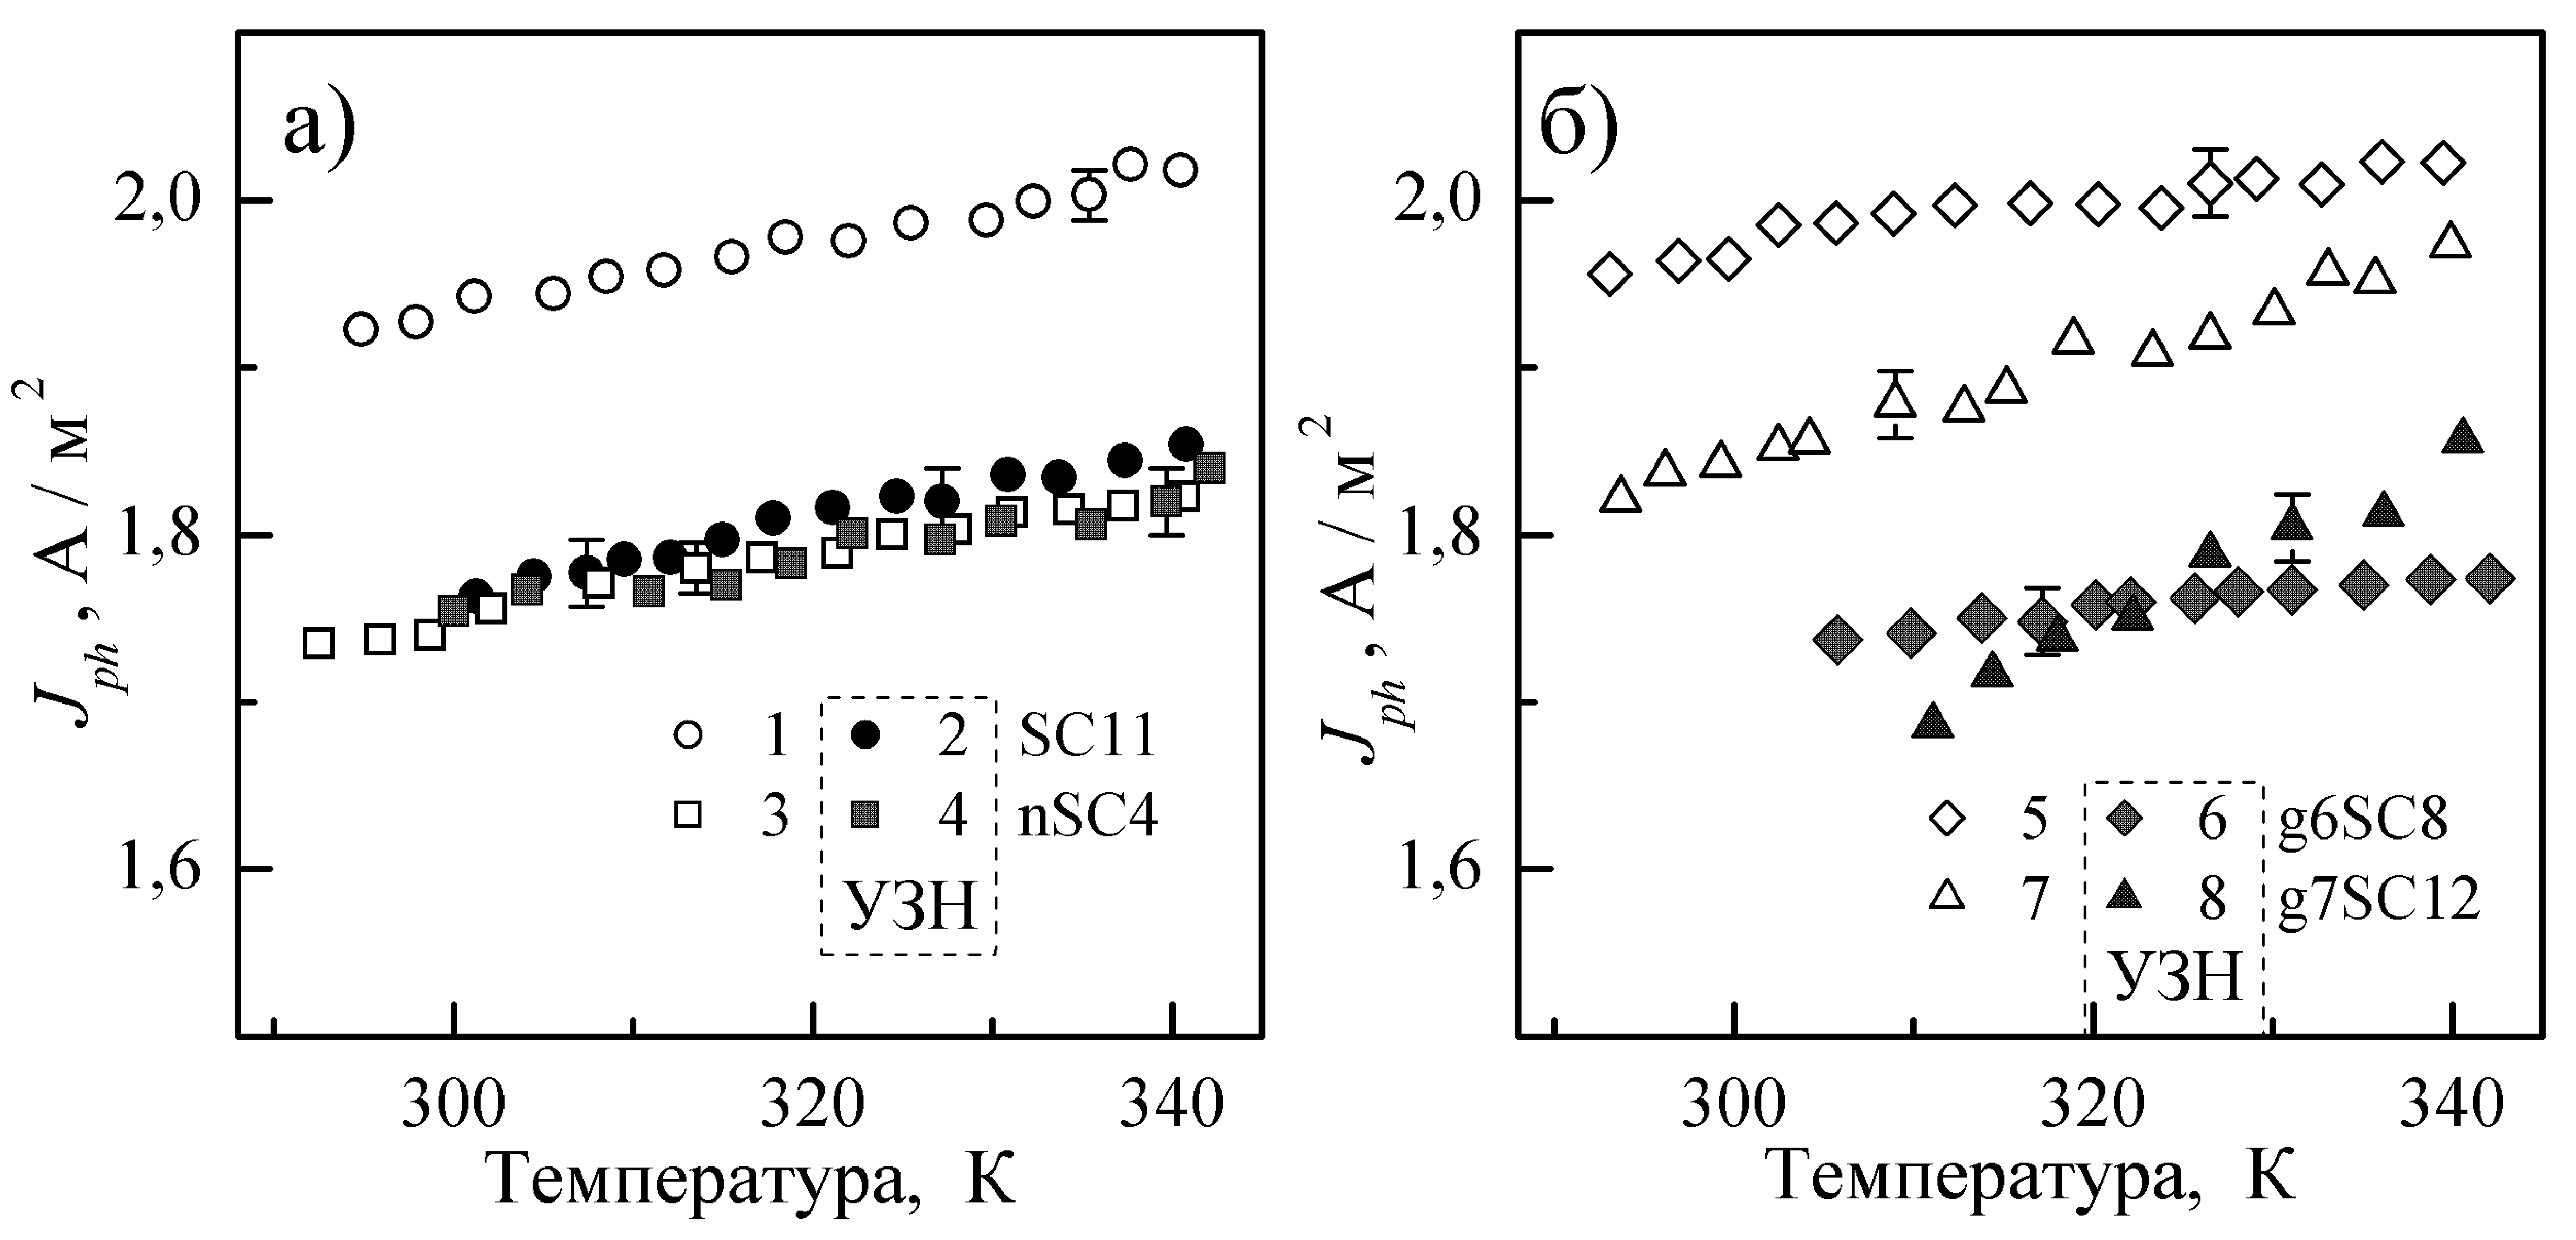
\includegraphics[width=1.0\textwidth]{figIscRD}
\caption{\label{figIscRD}
Температурні залежності густини фотоструму
для неопроміненого (криві 1 та 2, кола),
нейтронно--опроміненого (3 та 4, квадрати) та
гамма--опромінених (5--8, ромби та трикутники)
зразків.
Криві 1, 3, 5 та 7 (незаповнені точки) отримані без УЗН,
криві 2 та 4 відповідають УЗН U--Tb3,
6 та 8 ---
U--Tb2 та U--Tb1, відповідно.
}%
\end{figure}

З рисунка видно, що при збільшенні температури $J_{ph}$ зростає як до радіаційного впливу, так і після.
З літератури \cite{Faren,SCTemp:PP11,SCTemp:SEMSC140} відомо, що
подібна поведінка фотоструму зумовлена, переважно, двома факторами:
\begin{enumerate}[label=\arabic*),leftmargin=0em,itemindent=1.5em]
\item зменшення забороненої кристалу та зміною коефіцієнта поглинання світла;
\item збільшенням довжини дифузії неосновних носіїв заряду.
\end{enumerate}
Показано \cite{SCTemp:PP11,SCTemp:SEMSC140}, що при аналізі температурної залежності доцільно
розглядати густину фотоструму у вигляді
\begin{equation}
\label{eqIscIdeal}
J_{ph}=J_{Lg}f_c\,,
\end{equation}
де
$J_{Lg}$ --- ідеальне значення густини струму, яке визначається
зонною структурою кристалу,
$f_c$ --- коефіцієнт збирання (collection fraction),
який залежить від відбиття світла, його паразитного поглинання (особливо вільними носіями заряду)
та поширення носіїв у кристалі.
В цьому випадку температурний коефіцієнт фотоструму $\beta^T_{Jph}$ може бути записаний у вигляді
\begin{equation}
\label{eqIscTempKoef}
\beta^T_{Jph}=\frac{1}{J_{ph}}\frac{dJ_{ph}}{dT}=\frac{1}{J_{Lg}}\,\frac{dJ_{Lg}}{dE_g}\,\frac{dE_g}{dT}+\frac{1}{f_{f}}\frac{df_{c}}{dT}\,,
\end{equation}
причому перший доданок для кремнію у випадку сонячного освітлення становить близько $167\cdot10^{-6}$~K$^{-1}$.

Визначені з експерименту значення температурних коефіцієнтів наведено в Таблиці~\ref{tabIscT}.
Видно, що у всіх випадках зміна $J_{ph}$ з температурою визначається, насамперед,
зміною $f_c$, а величина $\beta^T_{Jph}$ практично не залежить від УЗН (за винятком інтенсивно опроміненого опроміненого гамма--квантами зразка).

\begin{table}
\caption{\label{tabIscT}Температурний коефіцієнт струму короткого замикання.
}
\center
\begin{tabular}{|c|c|c|c|}
\hline
Зразок&\multicolumn{2}{c|}{$\beta^T_{Jph}$, 10$^{-3}$K$^{-1}$}&УЗН\\ \cline{2-3}
&без УЗН & зі УЗН&\\ \hline
SC11&$1,3\pm0,2$&$1,2\pm0,2$&U--Tb3\\ \hline
nSC4&$1,1\pm0,2$&$1,3\pm0,3$&U--Tb3\\ \hline
g6SC8&$0,8\pm0,2$&$0,6\pm0,1$&U--Tb2\\ \hline
g7SC12&$1,6\pm0,2$&$3,1\pm0,4$&U--Tb1\\ \hline
\end{tabular}
\end{table}

На Рис.~\ref{figIscRD} звертає на себе увагу той факт, що у нейтронно--опроміненому
зразку фактично не спостерігається зміни величини фотоструму під дією УЗН.
Цей результат є досить несподіваним, враховуючи те, що, як було показано раніше,
УЗ викликає зменшення часу життя неосновних носіїв в КНО і в нейтронно--опроміненому зразку також ---
див. Рис.~\ref{figTAUrRD}, Таблицю~\ref{tabAIchangeRD}.
Причому ефективність АІ змін $\tau_n$ в нейтронно--опроміненому зразку навіть вища (Таблиця~\ref{tabAIchangeRD}, Рис.~\ref{figKusRD}),
що, як було показано в параграфі~\ref{sbRadDef}, зв'язано з акусто--активністю дивакансії.

На Рис.~\ref{figeIscRD} наведено більш детальне порівняння АІ змін фотоструму в нейтронно--опроміненому та неопроміненому
зразках при різних режимах УЗН з використанням повздовжніх хвиль.
З рисунка видно, $J_{ph}$ зменшується (нагадаємо, що, як і для всіх інших параметрів, $\varepsilon_{Jph}=(J_{ph,in}-J_{ph,\mathtt{US}})/{J_{ph,in}})$) при цьому
\begin{enumerate}[label=\asbuk*),leftmargin=0em,itemindent=1.5em]
\item зі збільшенням частоти УЗ ефективність змін фотоструму в неопроміненому КСЕ зростає;
\item навіть при високих частотах АІ ефект впливу УЗ на $J_{ph}$ в нейтронно--опроміненому КСЕ достатньо малий.
\end{enumerate}


\begin{figure}
\center
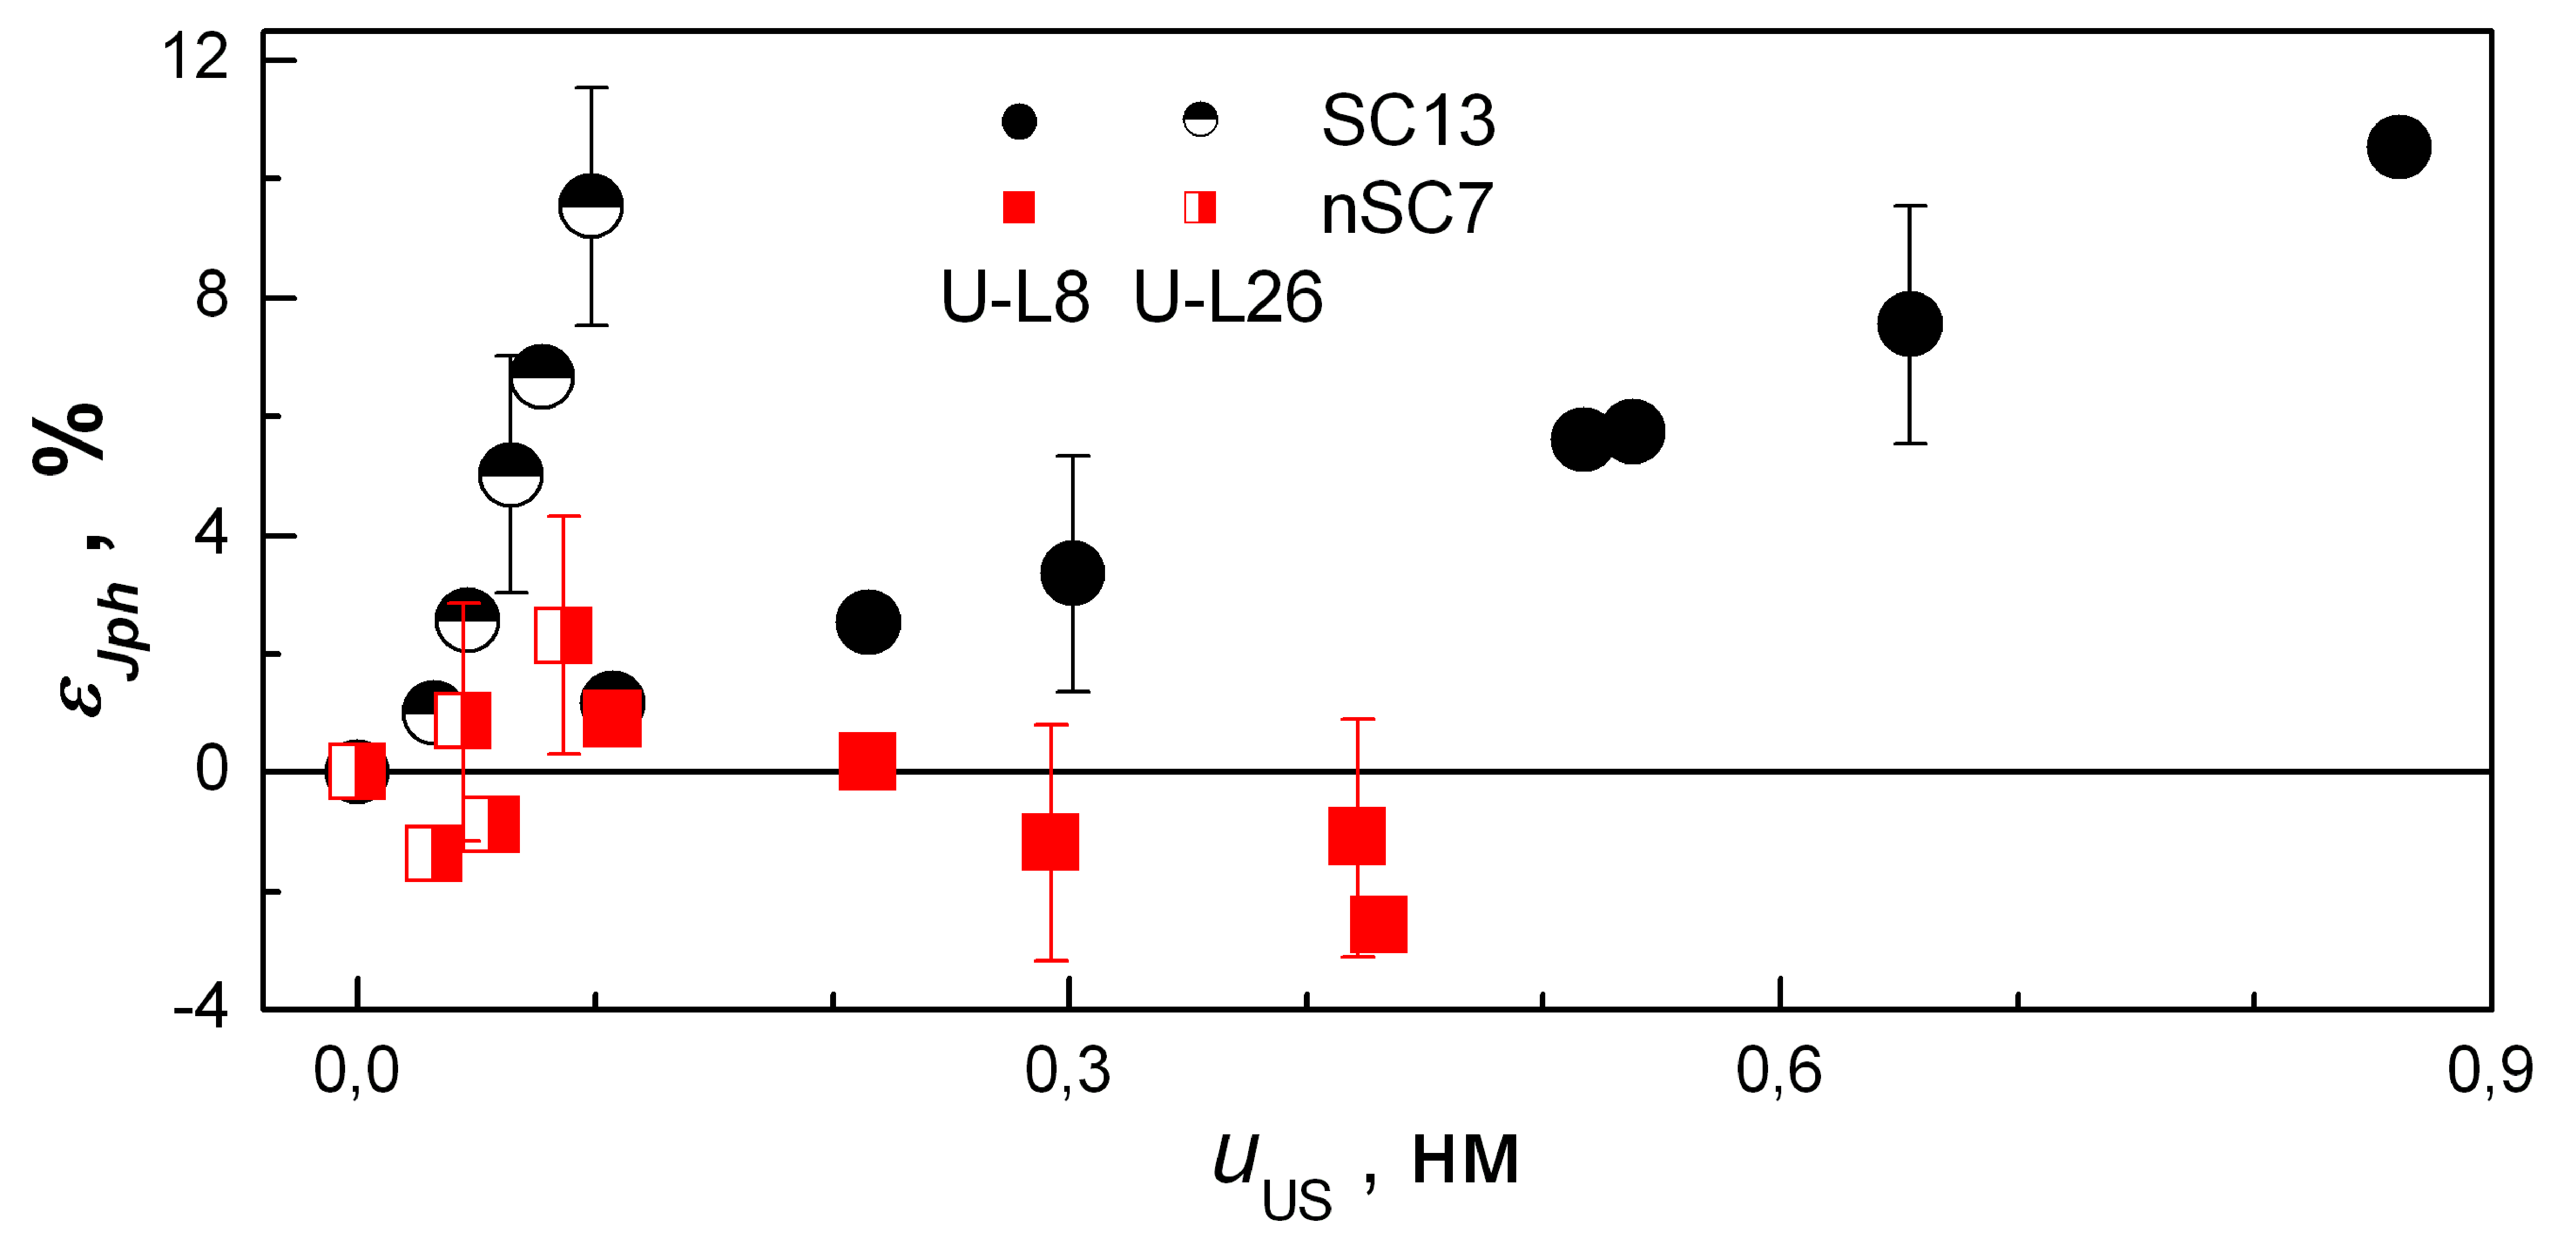
\includegraphics[width=1.0\textwidth]{figeIscRD}
\caption{\label{figeIscRD}
Залежності АІ змін фотоструму від
амплітуди зміщень атомів в неопроміненому (кола)
та опроміненому (квадрати) зразках.
$f_\mathtt{US}$, Гц: 8,0 (U--L8, заповнені точки),
26,1 (U--L26, напівзаповнені точки).
}%
\end{figure}

З метою більш детального вивчення виявленої особливості було проведено дослідження змін
довжини дифузії неосновних носіїв заряду.
Для визначення $L_n$ використовувався варіант методу SSSCC (steady--state short--circuit current)\cite{Schroder2006}.
А саме, як вже було згадано раніше, величина фотоструму в досліджених структурах
описується виразом (\ref{eqIph}).
Тобто, $J_{ph}$ має лінійно залежати від кількості фотонів
\mbox{$N_{ph}=W_{ph}\lambda /hc$}, які падають на поверхню структури за одиницю часу:
\begin{equation}
J_{ph}=K_{ph}N_{ph}\,,
\end{equation}
де коефіцієнт пропорційності
\begin{equation}
 K_{ph}=\frac{(1-R_{ph})\,q\beta \alpha L_n} {1+\alpha L_n}\,.
\end{equation}
Таким чином, знаючи коефіцієнти $K_{ph1}$ та $K_{ph2}$
для двох довжин хвиль $\lambda_1$ і $\lambda_2$, можна
визначити $L_n$:
\begin{equation}\label{F3}
L_n=\frac{(K_{ph1}\alpha_2)/(K_{ph2}\alpha_1)-1}{\alpha_2(1-K_{ph1}/K_{ph2})}\,,
\end{equation}
де $\alpha_1$ та $\alpha_2$ --- коефіцієнти поглинання для
світла з довжиною хвилі $\lambda_1$ та $\lambda_2$, відповідно.

В роботі використовувалися довжини світла 900 та 950 нм,
попереднє калібрування величини $W_{ph}$ здійснювалось
за допомогою германієвого фотодіоду 9Э111А.
На Рис.~\ref{figIscNph} показано типові залежності фотоструму від
кількості падаючих фотонів для двох довжин хвиль,
які дійсно були лінійні.
Зауважимо, що вираз (\ref{F3}) є справедливим,
за умови, що $R_{ph}$ та $\beta$ є однаковими для обох довжин.
Проте з літератури відомо, що для використаних довжин хвиль
$\beta=1$ \cite{Gaman}, а зміна коефіцієнту відбивання не перевищує 1\% \cite{GreenOptic,SiOptic:JAP1998,GreenOptic2}.
Таким чином, для визначення $L_n$ використовувалася формула (\ref{F3}),
причому $K_{ph1}$ та $K_{ph2}$ були виміряні експериментально, а значення
коефіцієнтів поглинання обчислювалися за допомогою виразу (\ref{eqAlpha}).

\begin{figure}
\center
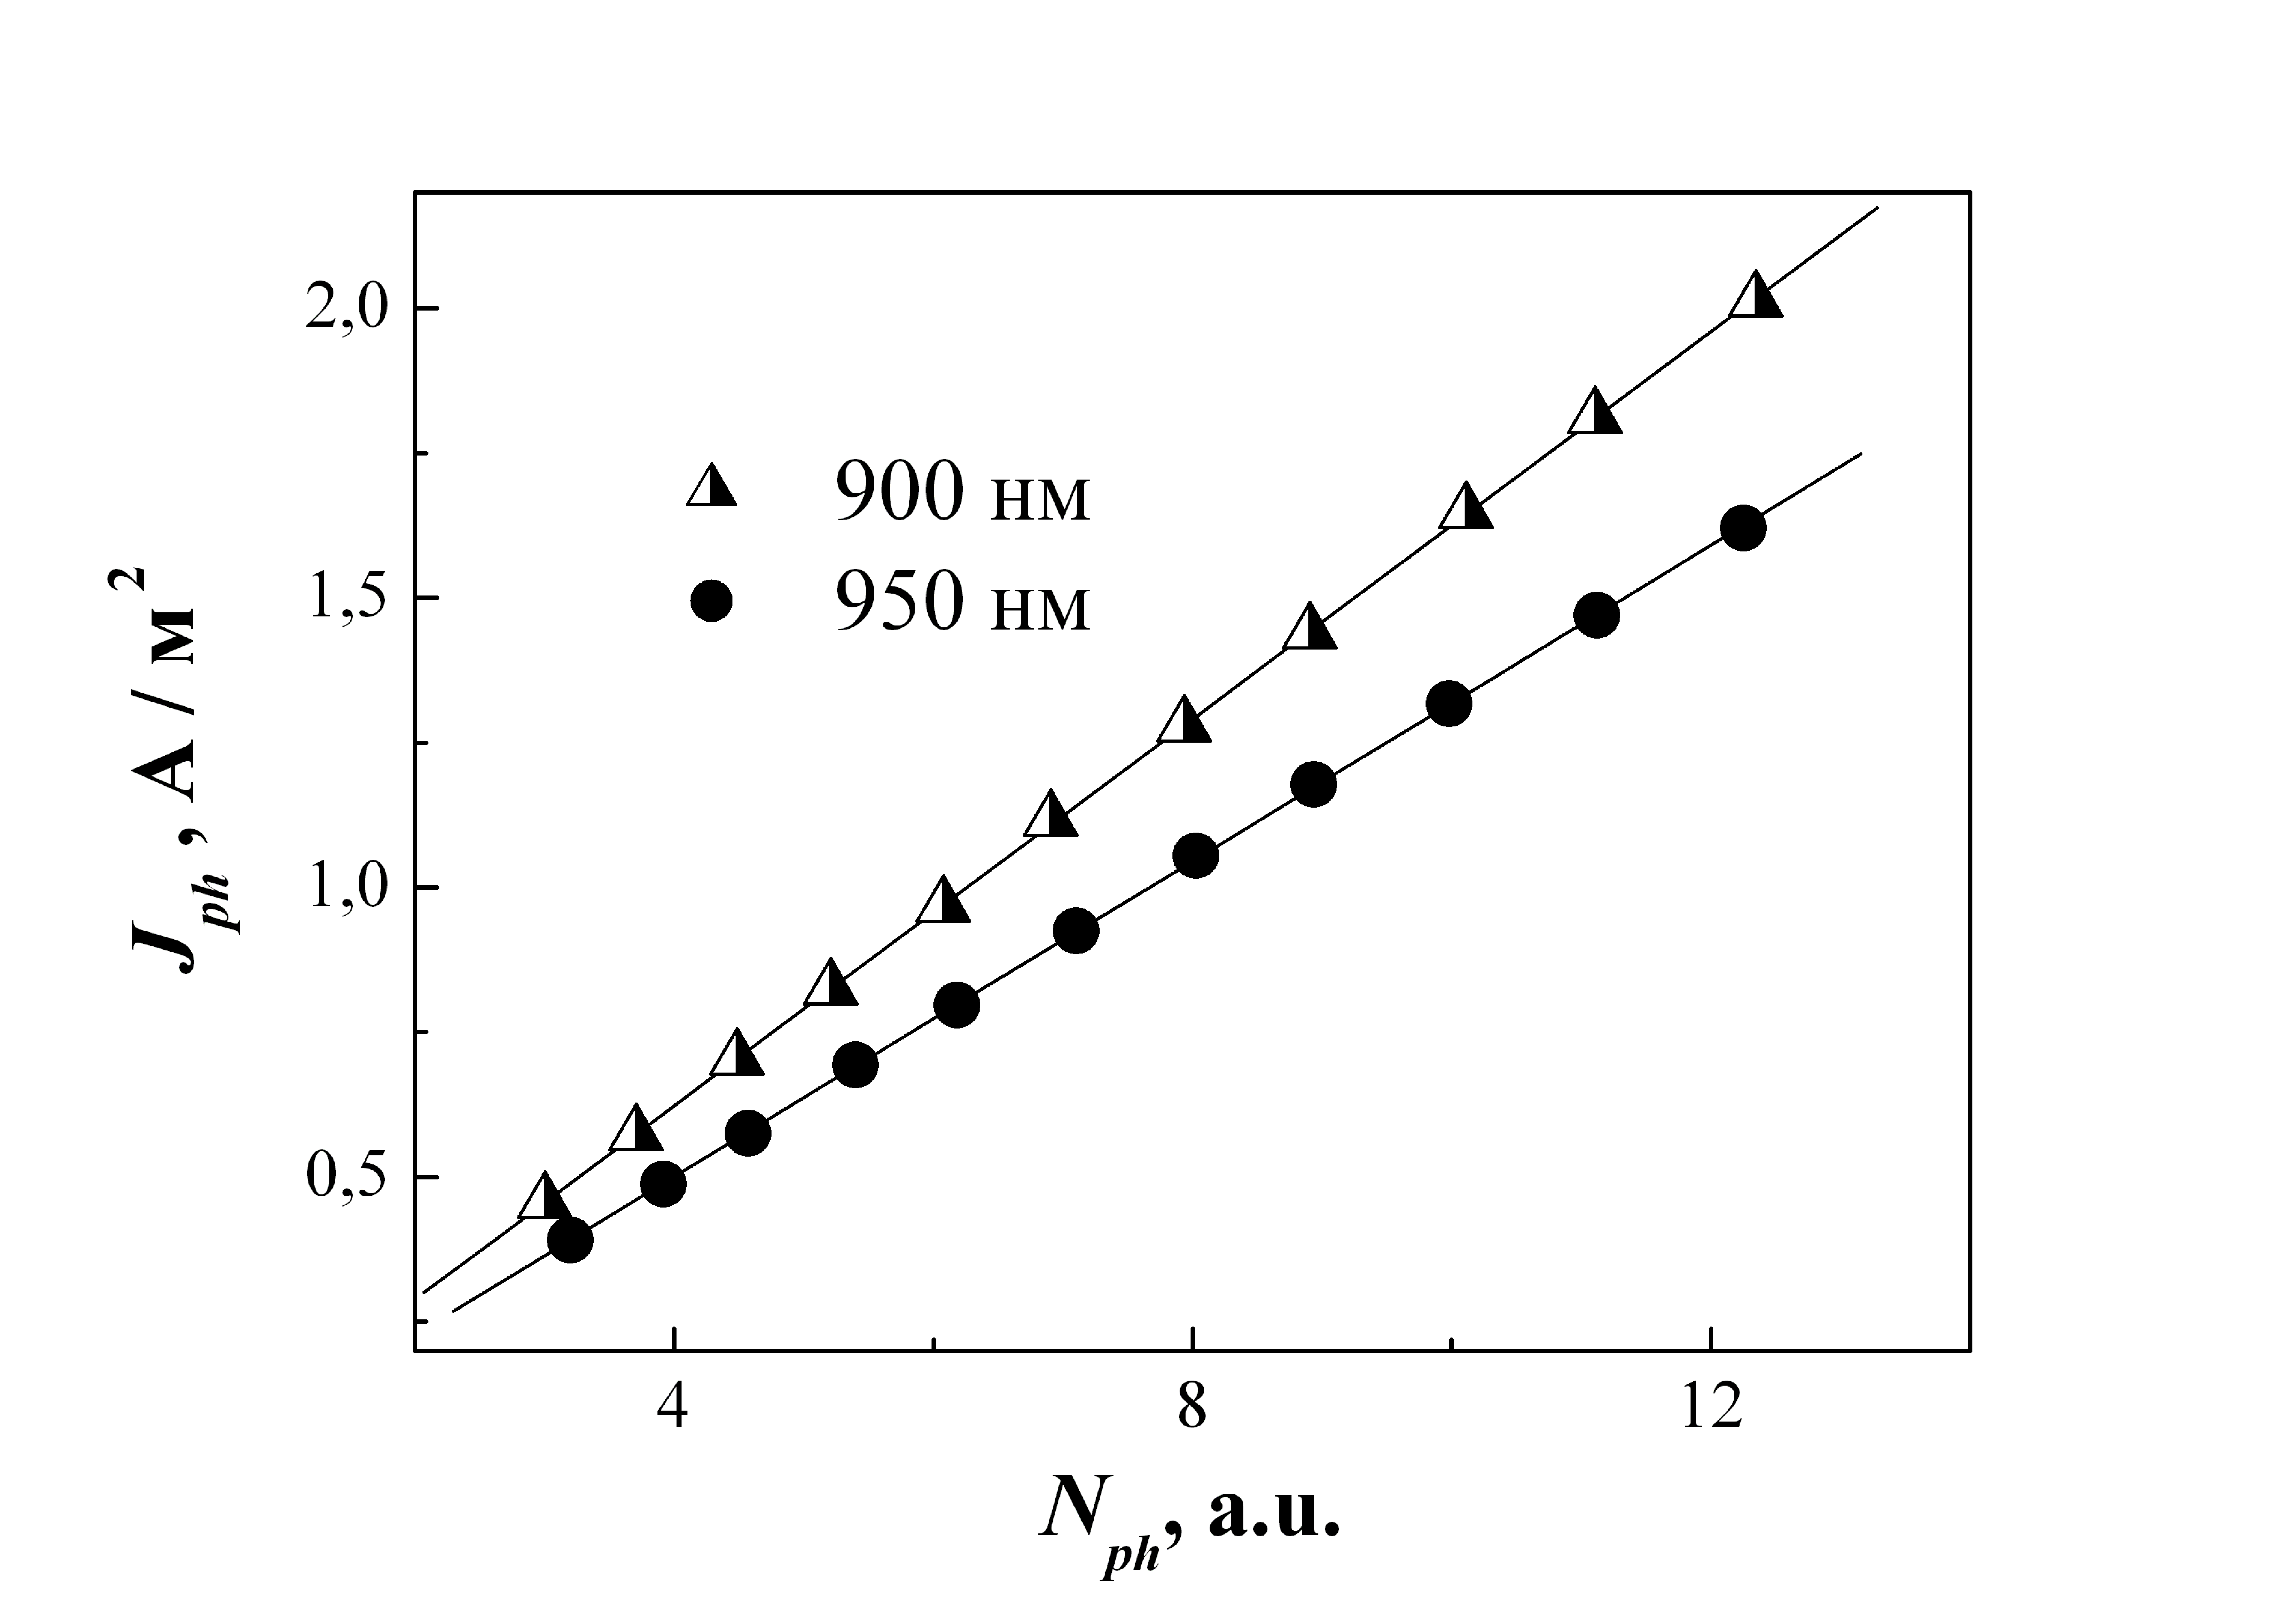
\includegraphics[width=0.7\textwidth]{figIscNph}
\caption{\label{figIscNph}
Залежність густини фотоструму від кількості падаючих фотонів.
Точки – експеримент, лінії – лінійна апроксимація.
$\lambda$, нм: 900 (трикутники), 950 (кола). Зразок SC13. $T = 290$~К.
}%
\end{figure}

З виразу (\ref{eqIph}) випливає, що при незалежності $R_{ph}$ від температури
зміна $J_{ph}$ має визначатися зміною
коефіцієнта $\Gamma=\alpha\,L_n/(1+\alpha\,L_n)$.
Було проведене порівняння відносних змін
фотоструму при нагріванні $\varepsilon^T_{Jph}=[J_{ph}(T)-J_{ph}(T_0)]/J_{ph}(T_0)$
($T_0=290$~K)
з відносними змінами цього коефіцієнта $\varepsilon_\Gamma=[\Gamma(T)-\Gamma(T_0)]/\Gamma(T_0)$,
при обчисленні якого використовувалися значення  $L_n$, визначені
для тих самих температур, при яких проводилось вимірювання $J_{ph}$.
Отримані результати показано на Рис.~\ref{figeIsceG}.


\begin{figure}
\center
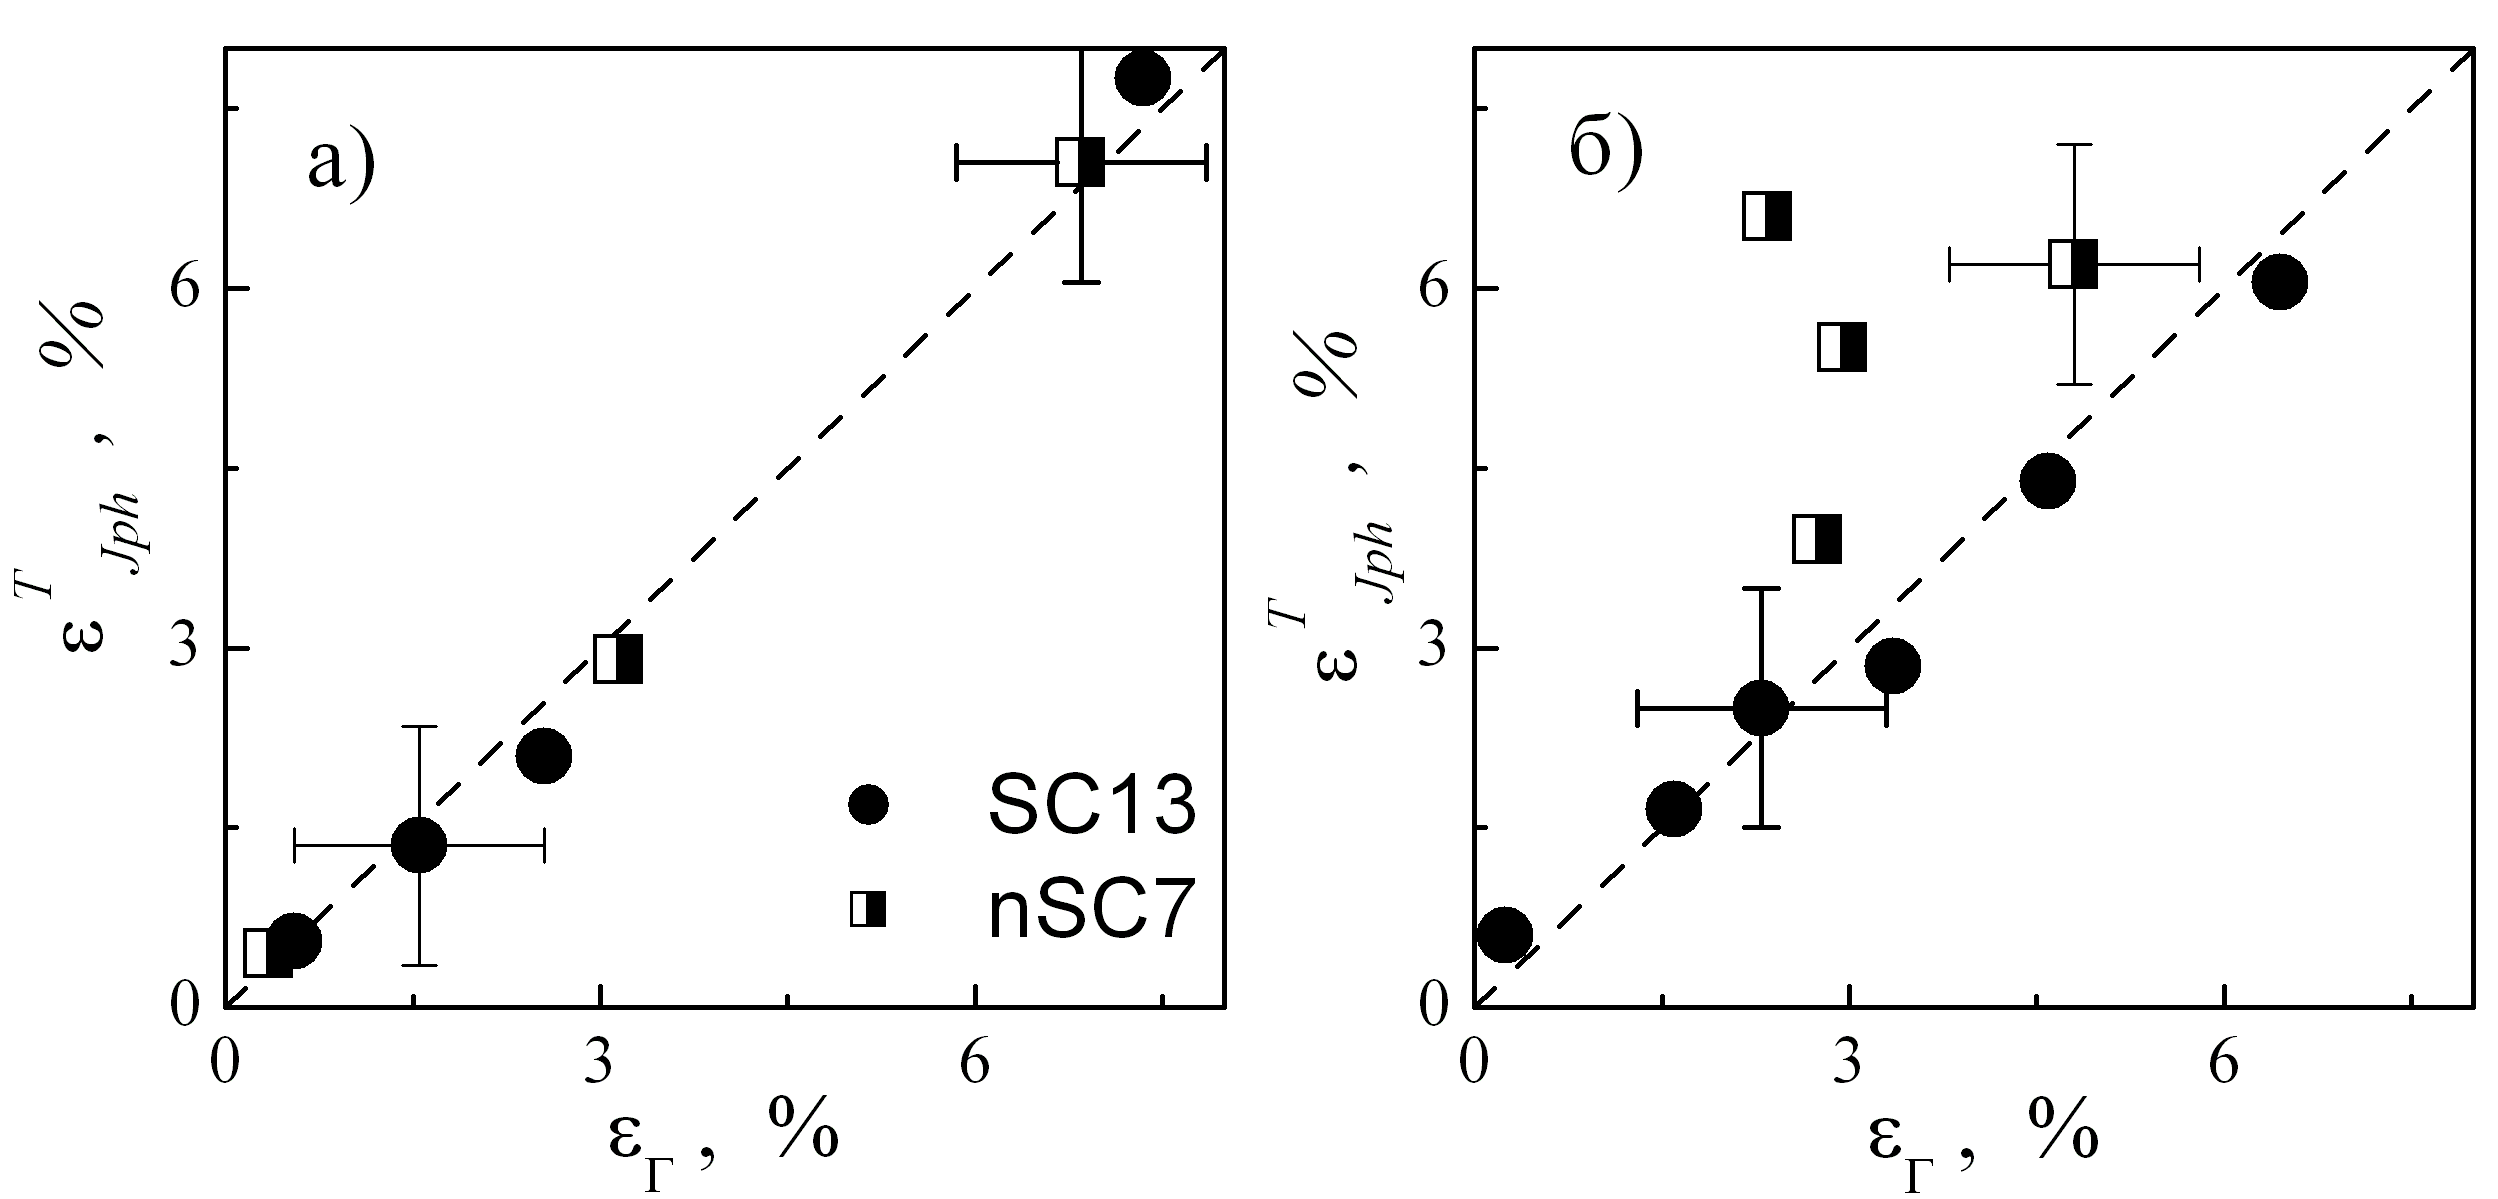
\includegraphics[width=1.0\textwidth]{figeIsceG}
\caption{\label{figeIsceG}
Порівняння відносних змін фотоструму зі змінами довжини
вільного пробігу неосновних носіїв заряду при беззвуковому
нагріванні (а) та нагріванні під час УЗН (U--L8, б)
для неопроміненого (кола) та опроміненого (квадрати) зразків.
}%
\end{figure}

Наведені дані показують, що при нагріванні за відсутності УЗН і для неопроміненого,
і для нейтронно--опроміненого зразка зміна фотоструму визначається зміною
$L_n$:
точки на Рис.~\ref{figeIsceG},а розташовані дуже близько до діагоналі.
Подібна картина спостерігається і для неопроміненого зразка в
умовах УЗН (Рис.~\ref{figeIsceG},б).
Тобто, зміна фотоструму в цьому випадку пов'язана з АІ зменшенням
довжини дифузії (часу життя) неосновних носіїв заряду в квазі--нейтральній
області внаслідок перебудови акусто--активних рекомбінаційних центрів ---
ефект, розглянутий раніше.
Збільшення ефективності АІ змін зі зростанням частоти УЗ, яке
спостерігається в експериментах, може бути пов'язане з наближенням
$f_\mathtt{US}$ до власних частот коливань домішкового комплексу.
Подібний резонансний характер АДВ спостерігався і раніше \cite{Ol_Shav}.




Водночас у нейтронно--опромінених структурах зміна фотоструму при УЗН більша,
ніж це можна очікувати виходячи зі значень зміни коефіцієнта $\Gamma$, пов’язаних з АІ зростанням $L_n$ --- Рис.~\ref{figeIsceG},б.
Це свідчить про існування додаткового механізму впливу УЗ на генерацію фотоструму в таких зразках.
Результатом дії цього механізму є збільшення величини $J_{ph}$, що повністю або частково компенсує
зменшення величини фотоструму внаслідок АІ збільшення активності рекомбінаційних центрів --- Рис.~\ref{figIscRD} та Рис.~\ref{figeIscRD}.
Водночас у структурах, опромінених $\gamma$--квантами даний механізм не відіграє суттєвої ролі.


Як видно з виразу~(\ref{eqIph}), однією з причиною цього може бути зменшення коефіцієнту відбивання від поверхні зразка.
В роботі~\cite{Zaver} наведені результати, які свідчать про те, що в результаті УЗО кремнію відбувається
зменшення $R_{ph}$ у спектральному
діапазоні, який використовувався в наших дослідах.
Проте мусимо зазначити, що цей ефект мав залишковий характер і
автори~\cite{Zaver} пов’язували його зі зменшенням концентрації
легуючої домішки у приповерхневому шарі напівпровідника внаслідок
її акусто--стимульованої дифузії вглиб кристалу.
В наших експериментах використовувалися АХ зі значно меншою потужністю, ніж
в~\cite{Zaver} (1 та 5 Вт/см$^2$, відповідно),  виявлені ефекти зміни фотоструму мали оборотний характер
і тому пов'язувати виявлений ефект з дифузією фосфору в УЗ полі не варто.
З іншого боку, відомо (див.,~наприклад,~\cite{Kizel}), що дефектний склад
приповерхневого шару суттєво впливає на процеси відбивання світла.
На нашу думку, утворені в результаті нейтронного опромінення порушення кристалічної ґратки
(насамперед, вакансійні кластери) є ААД.
Це підтверджується і попередньо наведеними даними, і результатами інших авторів \cite{YOlikh2006TPLr}.
АІ перебудова або зміна заселеності рівнів комплексів під час УЗН і спричинює зменшення коефіцієнта відбивання
і появу додаткового механізму зростання фотоструму.
До речі, такі процеси, а саме зменшення до 8\% $R_{ph}$ за рахунок зміни заселеності рівнів в
процесі акустичного навантаження спостерігалися раніше в
епітаксійних плівках GaAs \cite{Korotch}.
Іншою причиною зменшення
коефіцієнта відбивання може бути певне текстурування поверхні нейтронно-опромінених
структур в умовах УЗН.

Таким чином в результаті нейтронного опромінення може відбуватися
зміна просторового розташування області ефективної акусто-дефектної
взаємодії і дані процеси починають ефективно відбуватися також в
приповерхневому шарі напівпровідника.



\section*{Висновки до розділу \ref{Ch_SSC}}
\addcontentsline{toc}{section}{Висновки до розділу \ref{Ch_SSC}}
  \begin{enumerate}
     \item Проведено експериментальне дослідження впливу ультразвукового навантаження на параметри кремнієвих сонячних елементів
     у діапазоні температур $290\div340$~К.
     Виявлено, що при інтенсивності звуку менше $0,5$~Вт/см$^2$ спостерігається оборотна акусто--індукована деградація КСЕ.

     \item Проведено аналіз механізмів рекомбінації і показано, що в квазі--нейтральній області основним механізмом є рекомбінація Шоклі--Ріда--Хола,
     тоді як для області просторового заряду доцільно використовувати модель рекомбінації у системі спарених рівнів дефектів.

     \item Показано, що деградація фотоелектричних властивостей КСЕ пов'язана з акусто--індукованим зменшенням часу життя носіїв заряду,
     причому величина ефекту залежить, насамперед, від амплітуди коливань атомів, а вже потім від інтенсивності ультразвуку.

     \item Показано, що ефективність взаємодії акустичних хвиль з точковими дефектами зростає з підвищенням частоти коливань.

     \item Запропонована якісна модель акусто--активного комплексного дефекту, в рамках якого пояснено особливості спостережених ефектів.

     \item Досліджено можлива роль комплексів, які містять бор та кисень,
      пара залізо--бор та кисневмісних преципітатів у визначенні властивостей досліджених структур.
      Показано, що саме останні ефективно впливають на процеси рекомбінації та беруть участь у акусто--дефектній взаємодії.

     \item Виявлено, що в умовах акустичного навантаження збільшується внесок у рекомбінаційні процеси більш мілких рівнів, причому зміни величини відносних змін внесків різних центрів у загальну рекомбінацію практично лінійно залежать від амплітуди коливання атомів.
         Виявлено зменшення енергії термічної активації енергетичних рівнів, пов'язаних з дефектами, в умовах УЗН.

     \item Виявлено ефект акусто--індукованого зменшення шунтуючого опору в КСЕ.
      Показано доцільність використання моделі дислокаційно--індукованого імпедансу для пояснення температурних залежностей шунтуючого опору.
      Показано, що умовах ультразвукового навантаження збільшується ефективність захоплення носіїв заряду лінійними дефектами,
      розташованими в області $p$-$n$ переходу.

     \item Проведено експериментальне дослідження залежності впливу УЗН на параметри кремнієвих структур з $p$-$n$ переходом від
      опромінення реакторними нейтронами та $\gamma$--квантами $^{60}$Co.
      Виявлено, що в опромінених структурах спостерігається збільшення ефективності впливу ультразвуку
      на шунтуючий опір та час життя неосновних носіїв заряду в базі діоду.

     \item Виявлено, що акусто--індуковані оборотні зміни фактору неідеальності та часу життя носіїв в області просторового заряду
     мають різний знак в опромінених та неопромінених структурах.

     \item Показано, що виявлені ефекти в нейтронно--опромінених діодах пов'язані зі впливом ультразвуку на стан дивакансій,
     тоді як в гамма--опромінених діодах основним акусто--активним центром є комплекс вакансії та міжвузольного кисню.
     Отримані результати свідчать, що ультразвукове навантаженні викликає перебудову комплексу VO$_i$.
     Водночас виявлено, що комплекс з міжвузольного вуглецю та міжвузольного кисню практично не приймає участь у
     акусто--дефектній взаємодії.

     \item Вивлено, що вплив ультразвуку на фотогенерацію струму в нейтронно--опромінених
     кремнієвих $p$--$n$ структурах пов'язаний не лише з
     акустоіндукованою зміною неосновних носіїв заряду, але й існує альтернативний механізм, результатом дії
     якого є підвищення ефективності фото--електричного перетворення.
     Показано, що причиною подібних процесів може бути зменшення коефіцієнта відбивання світла в умовах ультразвукового навантаження.
     Таким чином в результаті нейтронного опромінення може відбуватися зміна просторового розташування області ефективної акусто-дефектної
     взаємодії і дані процеси починають ефективно відбуватися також і в
     приповерхневому шарі напівпровідника.

    \item Показано, що ультразвук може бути ефективним інструментом впливу на стан дефектів у кремнієвих структурах, а отже і на їх властивості.
  \end{enumerate}	

Основні результати даного розділу представлені в роботах
\cite{Olikh:Visn2003,Olikh:MRS2007,Olikh:SEMT2007,Olikh:FTP2009,Olikh:UPJ2010,Olikh:FTP2011,Olikh2018JAP,
1SEMST,2005IUS,ICU2007SC,2007MRS,3UNCPS,6Drog,4UNCPS,4Kremen,6SEMST,2017MEICS}.


\chapter{Порівняльний аналіз та оптимізація методів розрахунку параметрів структур метал--напівпровідник\label{Ch_MSMethod}}


\section{Загальні підходи до визначення параметрів діодів Шотки}
Напівпровідникові бар'єрні структури, як вже зазначалося раніше, надзвичайно широко застосовуються у техніці.
Параметри подібних структур є найбільш суттєвим фактором для можливості практичного використання,
а їх визначення відіграє надзвичайну важливу роль під час розробки, проектування та виготовлення пристроїв.
Одним з найпроширеніших шляхів визначення параметрів полягає у вимірюванні ВАХ.
В цьому випадку взаємозв'язок між струмом та напругою описується за допомогою певних фізичних моделей, в
результаті чого з'являється можливість вичленити параметри, спираючись на результати експериментальних вимірювань.
Наприклад, пряма гілка ВАХ ДШ згідно з моделлю термоемісії має описуватися \cite{Rhoderick1988} наступними виразами
\begin{eqnarray}
\label{eqSDIV}
I&=&I_s\left\{\exp\left[\frac{q(V-IR_s)}{n_\mathrm{id}kT}\right]-1\right\}\,,\\
\label{eqSDIs}
I_s&=&AA^*\,T^2\exp\left(-\frac{q\Phi_b}{kT}\right)\,,
\end{eqnarray}
де
$I_s$ --- струм насичення,
%$q$ --- елементарний заряд,
$R_s$ --- послідовний опір,
$n_\mathrm{id}$ --- фактор неідеальності,
%$k$ --- стала Больцмана,
%$T$ --- абсолютна температура,
%$A$ --- площа діоду,
$A^*$ --- ефективна стала Річардсона,
$\Phi_b$ --- висота бар'єру Шотки (ВБШ) при нульовому зміщенні.
$\Phi_b$ (або $I_s$), $n_\mathrm{id}$ та $R_s$ є найбільш фундаментальними параметрами даної моделі та повинні бути максимально точно визначені з експериментальних ВАХ.
В літературі запропоновано декілька методів визначення параметрів ДШ.
Найпростіший стандартний метод вимагає наявності лінійної області на залежності $\ln(I)$ від  $V$ \cite{Sze2012,Rhoderick1988}.
В цьому випадку два параметри, $n_\mathrm{id}$ та $\Phi_b$, можуть бути визначені за кутом нахилу та перетином  залежності з віссю струмів, відповідно.
На жаль, подібний підхід перестає бути дієздатним у випадку, коли структура характеризується значним послідовним опором.
Зокрема, рівняння~(\ref{eqSDIV}) перетворюється у трансцендентне, що суттєво ускладнює математичні аспекти визначення параметрів.
З одного боку, існує цілий набір аналітичних методів екстраполяції параметрів ДШ.
%Зважаючи на складність задачі, існує цілий ряд методів, які вирішують задачу екстраполяції параметрів ДШ.
Вони базуються на безпосередніх алгебраїчних наближеннях і використовують різноманітні допоміжні функції \cite{Norde,Lien,Werner,Cheung,Gromov,Lee,Bohlin,Cibils,Manifacier},
процедури  диференцювання  \cite{Mikhelashvili} або інтегрування  \cite{Kaminski,Ortiz1995,Durmus} ВАХ,
розбиття діапазону напруг на декілька частин \cite{Cataldo},
вимірювання ВАХ при декількох температурах \cite{Sato} або з використанням додаткового зовнішнього опору \cite{Lyakas}.


З іншого боку, визначення параметрів є багатовимірною задачею чисельної оптимізації і тому для її вирішення запропоновані різноманітні чисельні методи \cite{Ortiz1999,Evangelou,Donoval,Ferhat}.
Зазвичай, вони використовують метод найшвидшого градієнтного спуску для мінімізації різниці між виміряними та апроксимуючими значеннями.
При цьому деякі автори\cite{Lambert_Jung,Ortiz2005} шукають розв'язок рівняння~(\ref{eqSDIV}) використовуючи $W$--функцію Ламберта
\cite{LambertBook}.
Зазвичай, чисельні методи характеризуються більш високим рівнем достовірності визначення параметрів, проте нерідко вимагають відносно довгого часу для розрахунку.
Крім того, спостерігається тенденція збіжності у локальний екстремум замість глобального.

Нарешті, порівняно нещодавно було запропоновано використовувати еволюційні алгоритми (ЕА) для визначення параметрів напівпровідникових пристроїв \cite{PSO_Ye,DEWang,GA_Li,P-DE_Ishaque,TLBO_Patel,MABC,PSOWang,GA_Schottky}.
ЕА це стохастичний метод, який виявляє дуже високу ефективність при оптимізації дійсних цільових функцій багатьох змінних.
На відміну від чисельних методів, ЕА може бути застосований до нелінійних функцій без необхідності розрахунку похідних, а також слабко залежить від початкових наближень значень параметрів.
ЕА вважаються \cite{P-DE_Ishaque} найбільш багатообіцяючими  методами розрахунку параметрів.

Про важливість задачі визначення параметрів ДШ свідчить хоча б той факт, що
незважаючи на досить тривалу історію вивчення цього питання і накопичений достатньо широкий асортимент методів вирішення цього завдання,
в літературі постійно з'являються пропозиції щодо нових варіантів методів.
Наприклад, серед подібних робіт лише у другій половині 2017~року можна виділити \cite{Noise:Roy,MikhelashviliJAP2017,Cataldo}.

У літературі наявні роботи \cite{Evangelou,Aubry,Kudryk}, в яких проводиться порівняння  та огляд шляхів визначення параметрів ДШ, проте вони переважно зосереджені на розгляді лише декількох метод і фактично не беруть до уваги еволюційні алгоритми.
Задача, яка вирішувалась під час досліджень, описаних у даному розділі, полягала у порівнянні ефективності (точності визначення параметрів та швидкості роботи) різних методів визначення параметрів МН--структур з ВАХ.
Крім того, розглянуте питання впливу величини окремих параметрів на точність визначення всього набору.
Було розглянуто підгрупу методів, які дозволяють визначити $\Phi_b$, $n_\mathrm{id}$ та $R_s$ використовуючи лише одну ВАХ.
Зокрема, увага сфокусована на 10 аналітичних методах, 2 чисельних методах та 4 еволюційних алгоритмах
(диференційної еволюції (DE, differential evolution),
оптимізації зграї частинок (PSO, particle swarm optimization),
модифікованої штучної бджолиної сім'ї (MABC, modified artificial bee colony) та
оптимізованого викладання та навчання (TLBO, teaching learning based optimization)).


%Основні результати даного розділу представлені в роботах \cite{Olikh:Rev,6CPFCS}.

\section{Контрольні вольт--амперні характеристики}
Досліджені методи були застосовані до наборів ВАХ, отриманих як експериментально, так і синтезованих штучно.
В останньому випадку використовувалися як ідеальні характеристики, так і криві з певним рівнем шуму, який віддзеркалював можливість наявності випадкових похибок вимірювань у реальних умовах.

\subsection{Ідеальні синтезовані ВАХ\label{SubData}}
Переважно, для оцінки спроможності визначення параметрів структур МН за допомогою аналітичних \cite{Norde,Lien,Werner,Gromov,Lee,Bohlin,Cibils,Mikhelashvili,Kaminski} та чисельних \cite{Evangelou,Donoval} методів, а також еволюційних алгоритмів \cite{PSO_Ye,P-DE_Ishaque,TLBO_Patel} використовують структури на основі кремнію.
Керуючись таким загальноприйнятим підходом, під час синтезу ВАХ вважалося, що використовуються кремнієвий ДШ.
ВАХ були розраховані за допомогою рівняння ~(\ref{eqSDIV}), для розв'язку якого застосовувався метод дихотомії \cite[с.~158]{KalitkinBook}.
При цьому використовувалися значення $A=3,14\cdot10^{-6}$~м$^2$ та $A^*=112$~A$\,$cм$^{-2}$K$^{-2}$ (випадок $n$--Si \cite{Schroder2006}).
Напруга змінювалась з кроком 0,01~В, струм вар'ювався в діапазоні $10^{-9}\div10^{-2}$~A.

Задача полягала у перевірці ефективності методів при різних значеннях параметрів і тому дані були синтезовані для діапазону температур від 130 до 330~К.
В той же час, ми намагались синтезувати ВАХ, які близькі до характеристик реальних діодів.
Тому температурні залежності $\Phi_b$, $n_\mathrm{id}$ та $R_s$ були обрані, спираючись на наступні міркування.
Як передбачено теорією \cite{Rhoderick1988} та спостережено на експерименті \cite{Aboelfotoh,Zhua},
для випадку однорідного контакту Шотки ВБШ має зменшуватись з підвищенням температури, причому очікувана залежність подібна до температурної залежності ширини забороненої зони напівпровідника.
Тому для апроксимації температурної залежності ВБШ використовувалося рівняння Варшні \cite{SiEg2012}
\begin{equation}
\label{eqFbT}
\Phi_b(T) = \Phi_b(0) - \frac{7,021\cdot10^{-4} T^2}{T + 1108} ,
\end{equation}
причому вважалося, що ВБШ при нульовій температури $\Phi_b(0)=0,75$~еВ.
Температурна залежність фактору неідеальності нерідко описується співвідношенням
\begin{equation}
\label{eqnT}
n_\mathrm{id}=1+\frac{T_0}{T},
\end{equation}
де величина константи $T_0$ для випадку кремнію знаходиться в діапазоні $20\div50$~K \cite{T0:Lee,T0:McCafferty,T0:Saxena,Aboelfotoh}.
Для синтезу ВАХ було використане значення $T_0=35$~K.
Температурна залежність послідовного опору може бути описана виразом \cite{Sze2012,Rs:Meyaard,Rs:Kang}
\begin{equation}
\label{eqRsT}
R_s=R_{s0}\exp\left(\frac{E_a}{kT}\right),
\end{equation}
де $E_a$ -- енергія активації легуючої домішки.
В роботі були використані значення $E_a=0,044$~еВ (що відповідає домішковому атому фосфору) та $R_{s0}=0.25$~Ом.

Як наслідок, набір синтезованих для аналізу ВАХ складався з 21 кривої, які відповідали інтервалу температуз $130\div330$~К з кроком 10~К.
При цьому  $\Phi_b$, $n_\mathrm{id}$ змінювались $R_s$ від 0,740 до 0,697~еВ, від 1,27 до 1,11 та від 12,6 to 1,2~Ом, відповідно.


\subsection{Синтезовані ВАХ з випадковими похибками}
Для того, щоб моделювати можливі випадкові похибки, які виникають під час вимірювань, та проаналізувати стійкість методів визначення параметрів до їх наявності,
були також синтезовані набори ВАХ, в яких значення напруги та струму вибиралися з певним рівнем шуму.
В цьому випадку напруга $V_i$ та струм $I_i$, які відповідали $i-$й точці ВАХ вибиралися випадковим чином використовуючи розподіл Гауса.
Тобто, густина ймовірності очікування певної величини напруги описувалася виразом
\begin{equation}
\label{eqGaus}
f(V_i,\overline{V}_i,\sigma_V)=\frac{1}{\sigma_V\sqrt{2\pi}}\exp\left[-\frac{(V_i-\overline{V}_i)^2}{2\sigma_V^2}\right].
\end{equation}
При цьому середнє значення (сподівання) напруги $\overline{V}_i$ змінювалося з кроком 0,01~В,
середнє значення сили струму $\overline{I}_i$ обчислювалося використовуючи рівняння~(\ref{eqSDIV}) та $\overline{V}_i$.
Стандартне відхилення (дисперсія) напруги $\sigma_V$ вибиралася сталою для всього набору (21 криві) ВАХ.
Стандартне відхилення сили струму $\sigma_I$ залежало від величини сили струму $\sigma_I=\sigma_I^\varepsilon\cdot\overline{I}_i$,
де постійна для набору ВАХ величина $\sigma_I^\varepsilon$ --- відносна дисперсія струму.
Такий підхід відповідає достатньо поширеному на практиці випадку, коли відносні похибки вимірювання напруги та струму залишаються сталими для всієї ВАХ.
Надалі для позначення синтезованих подібним чином ВАХ буде використовуватися термін "зашумлені синтезовані дані" (noisy synthetic data).

Різні набори синтезованих ВАХ відрізнялися значеннями $\sigma_V$ та $\sigma_I^\varepsilon$.
Фактично, для ідеальних синтезованих ВАХ $\sigma_V=0$~В and $\sigma_I^\varepsilon=0$.


\subsection{Експериментальні ВАХ}
Досліджені методи були застосовані також до експериментально виміряних ВАХ кремнієвих структур SSDA, описаних в параграфі~\ref{MSSi}.
Параметри ДШ визначались на основі характеристик, отриманих в інтервалі температур $130\div330$~К, який збігався з діапазоном синтезованих ВАХ.

\section{Критерії точності методів}
У випадку, коли методи застосовувалися для аналізу синтезованих ВАХ, проводилося оцінювання похибок визначення параметрів.
Зокрема, для кількісної оцінки точності кожного з методів використовувалися наступні величини.
Оцінювання визначення фактору неідеальності з однієї ВАХ $\chi^q_n$ здійснювалося за допомогою виразу
\begin{equation}
\label{eqniac}
\chi^q_n=\left(\frac{n_{\mathrm{id},ext}-n_{\mathrm{id},ac}}{n_{\mathrm{id},ac}}\right)^2,
\end{equation}
де
$n_{\mathrm{id},ext}$ --- значення, отримане в результаті застосування методу,
$n_{\mathrm{id},ac}$ --- точне значення, яке використовувалося під час синтезу ВАХ.


Похибка визначення $n_\mathrm{id}$ на всьому наборі ВАХ $\varepsilon_n$ обчислювалася  як квадратних корінь з середньо--геометричного значення $\chi^q_n$:
\begin{equation}
\label{eqnac}
\varepsilon_n=\sqrt[2N_{I\!V}]{\prod_{i=1}^{N_{I\!V}}\chi^q_{n,i}},
\end{equation}
де
$N_{I\!V}$ --- загальна кількість ВАХ у наборі.
Для оцінювання похибки визначення ВБШ та послідовного опору з однієї ВАХ використовувалися величини  $\chi^q_\Phi$ та $\chi^q_R$, а для набору ВАХ --- $\varepsilon_\Phi$ and $\varepsilon_R$, для розрахунку яких використовувалися вирази, аналогічні (\ref{eqniac}) та (\ref{eqnac}), відповідно.

\section{Методи визначення параметрів діодів Шотки}
\subsection{Аналітичні методи\label{AnMethod}}
Модифікований метод Норда \cite{Norde,Lien,Sato,Dermircioglu:Norde} базується на використанні допоміжної функції
\begin{equation}
\label{eqNorde}
F(V)=\frac{V}{\gamma_N}-\frac{kT}{q}\ln\left(\frac{I(V)}{AA^*T^2}\right),
\end{equation}
де
$\gamma_N$ --- довільна константа, яка має бути більша, ніж фактор неідеальності.
При цьому величини ВБШ та послідовного опору визначаються за допомогою співвідношень
\begin{eqnarray}
\label{eqNordDet}
\Phi_b&=&F(V_{min})+\frac{\gamma_N-n_\mathrm{id}}{n_\mathrm{id}}\left(\frac{V_{min}}{\gamma_N}-\frac{kT}{q}\right),
\\
R_s&=&\frac{(\gamma_N-n_\mathrm{id})kT}{qI_{min}}\,,
\end{eqnarray}
де
$F(V_{min})$ та $V_{min}$ --- це координати точки мінімуму залежності $F(V)$ від $V$;
$I_{min}$  --- струм, який на ВАХ відповідає $V_{min}$.

Необхідно підкреслити, що згідно з цим методом, значення $n_\mathrm{id}$ має бути відомим.
Як наслідок, при застосування метода Норда до синтезованих та експериментальних ВАХ, використовувалися величини $n_{\mathrm{id},ac}$ та значення, отримане з використанням методу MABC, відповідно.

Крім того, для випадку  $R_s<5$~Ом, мінімум функції Норда $F(V)$, побудованої на основі ВАХ в діапазоні струмів до $10^{-2}$~А, не спостерігався взагалі.
Тому при застосуванні цього методу, так і методу Бохліна (описаного нижче), використовувалися набори ВАХ, синтезовані в більш широкому струмовому діапазоні, від $10^{-9}$ до $10^{-2}$~A.

Нарешті, проведені розрахунки показали, що точність методу Норда залежить від вибраної величини $\gamma_N$.
Відповідні залежності наведено на Рис.~\ref{figNorde}.
Зокрема показано, що похибка визначення $\Phi_b$ збільшується зі зростанням $\gamma_N$ як для випадку ідеальних синтезованих ВАХ, так і при використанні зашумлених даних.
В той же час, похибка визначення  $R_s$
а)~зменшується зі зростанням $\gamma_N$ при $\gamma_N<2$ і залишається сталою при $\gamma_N>2,5$ для зашумлених даних;
б)~немонотонно залежить від $\gamma_N$ для ідеальних синтезованих ВАХ.
Враховуючи виявлені суперечливі тенденції для мінімізації похибки методу Норда при отриманні наведених надалі даних використовувалося значення $\gamma_N=1,8$.

Для позначення результатів, отриманих з використанням методу Норда, використовується мітка <<Norde>>.

\begin{figure}
\center
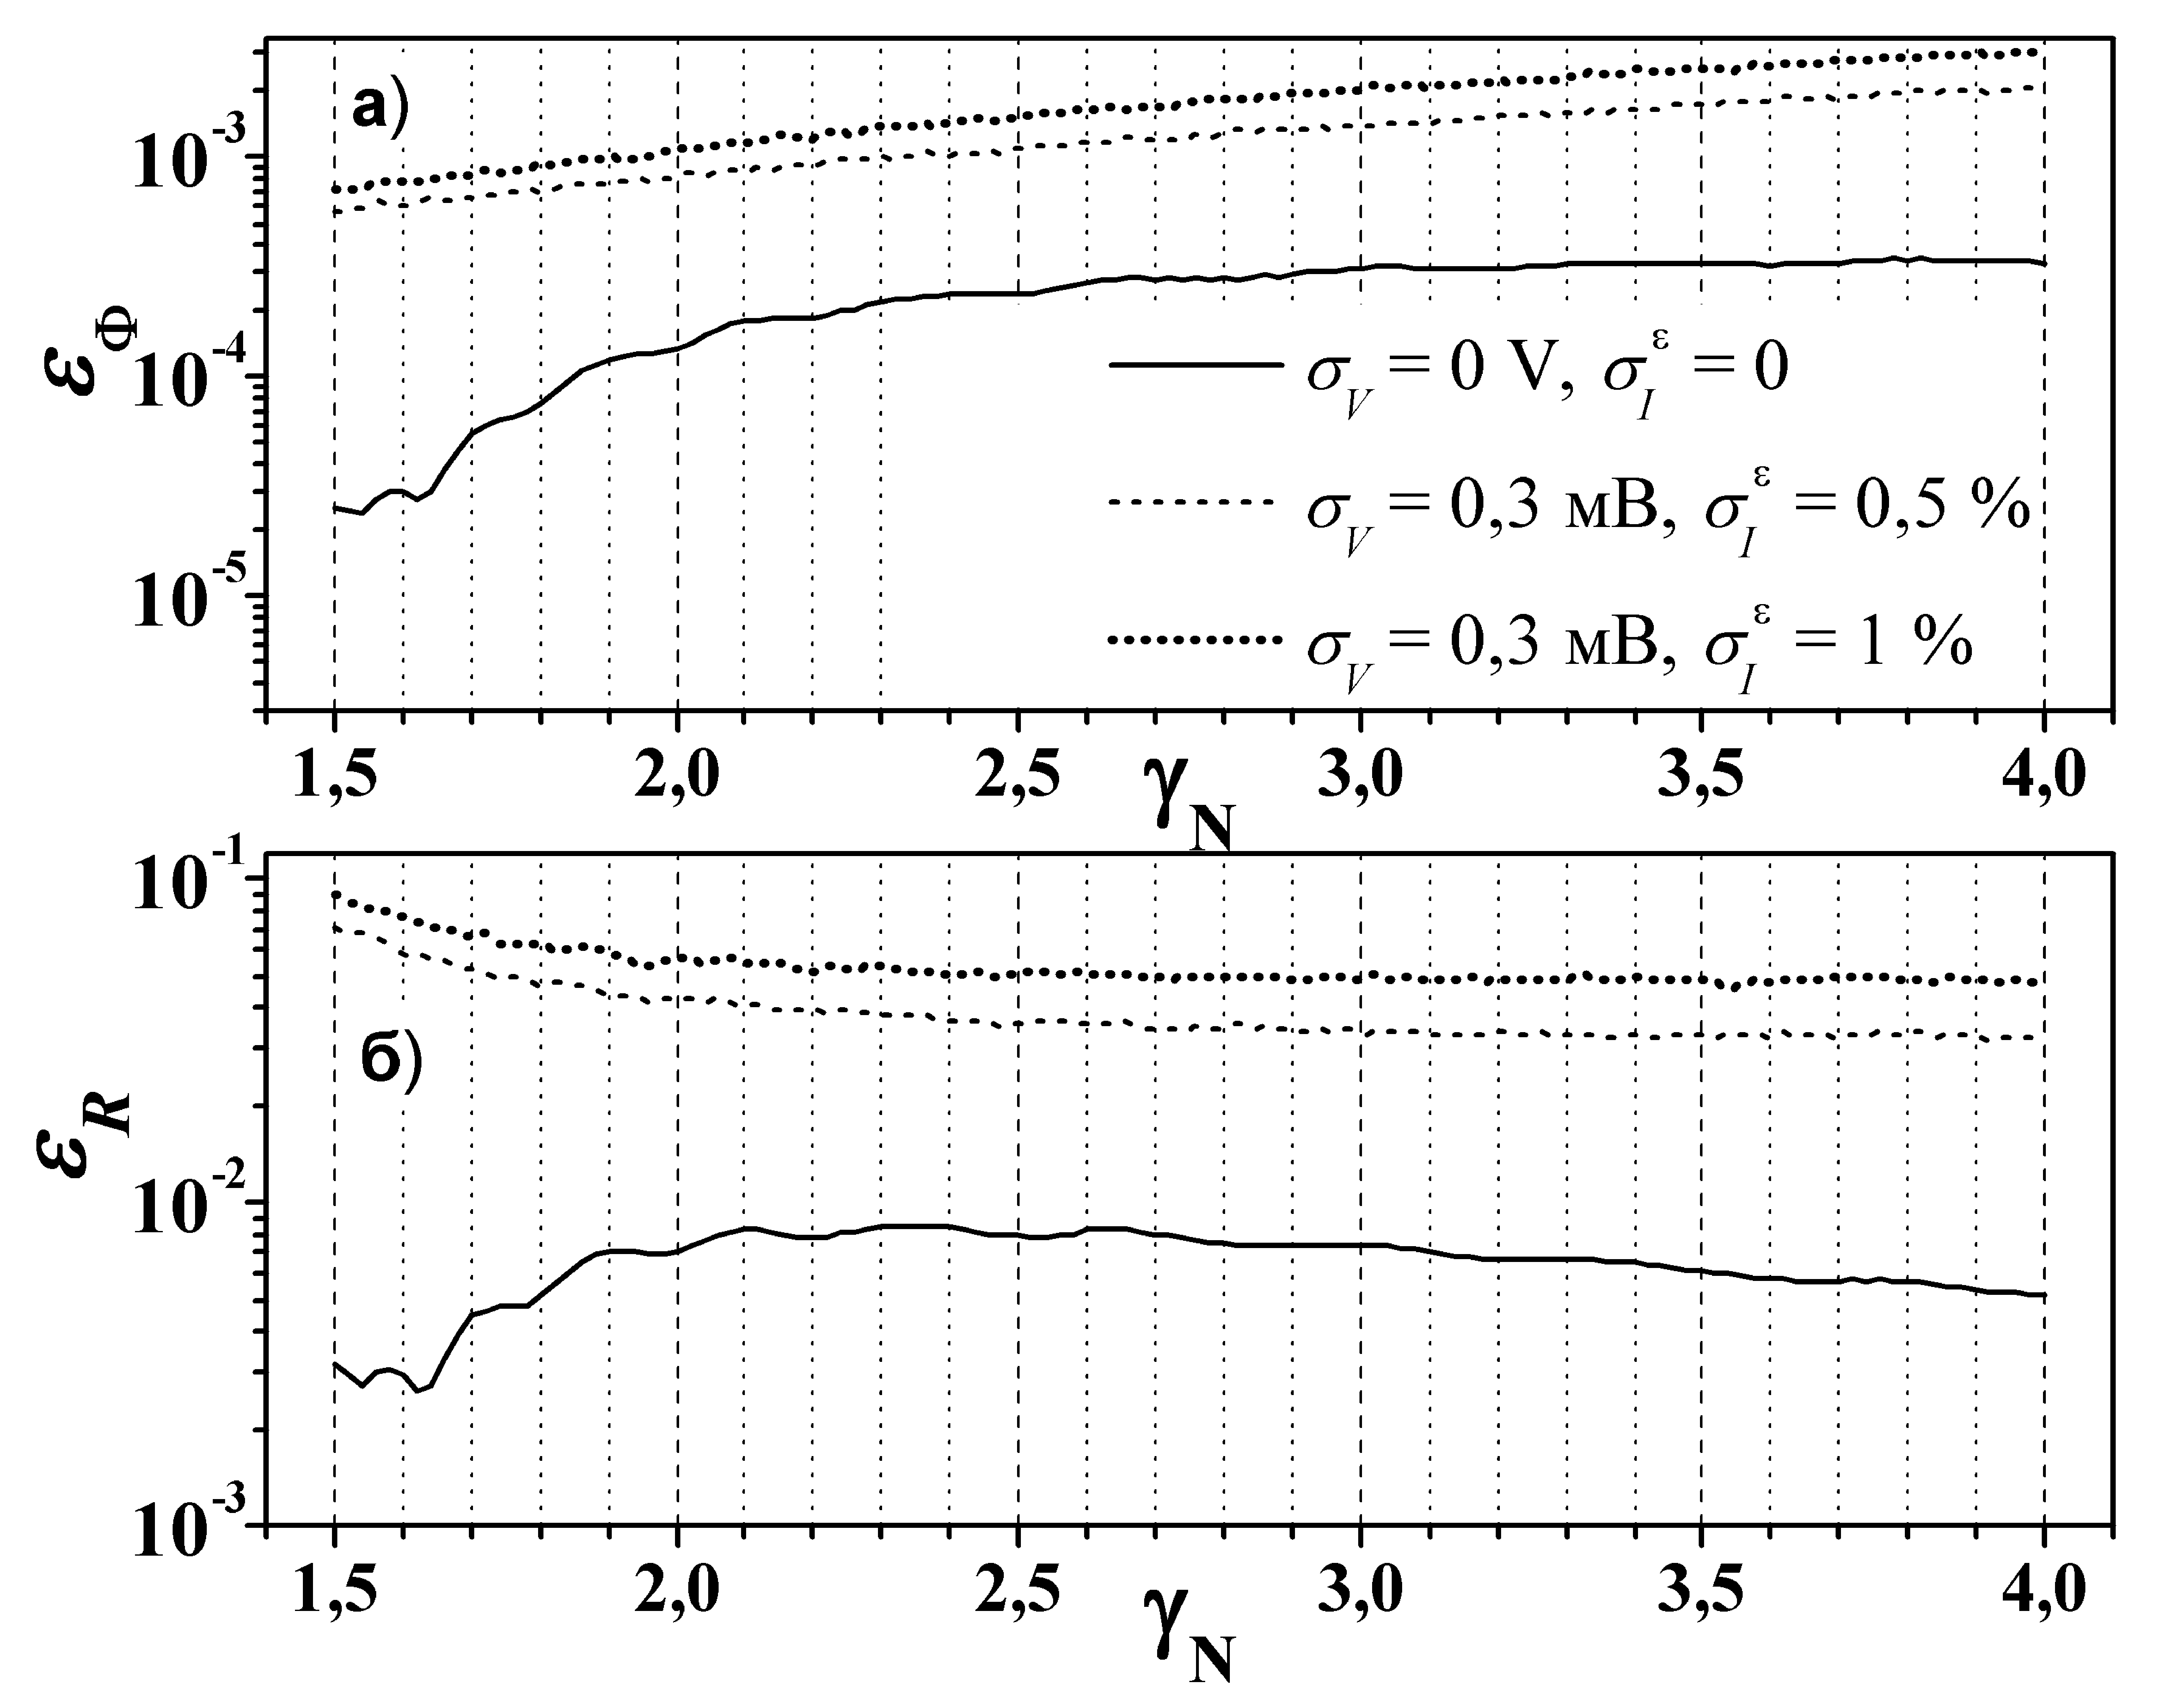
\includegraphics[width=0.6\textwidth]{figNorde}%
\caption{\label{figNorde}
Залежності похибки визначення $\Phi_b$ (a) та $R_s$ (б)  від величини $\gamma_N$.
 при застосуванні метода Норда до набору ідеальних синтезованих ВАХ (суцільні лінії) та зашумлених даних (штрихові лінії).
}
\end{figure}

J.~Werner  \cite{Werner} показав, що за умови коли падіння напруги в області бар'ру $V_d=(V-IR_s)\gg nkT/q$, то
\begin{equation}
\label{eqWerner}
\frac{(dI/dV)}{I}=\frac{q}{nkT}\left[1-R_s\left(\frac{dI}{dV}\right)\right].
\end{equation}
Рівняння~(\ref{eqWerner}) показує, що графік  залежності   $(dI/dV)/I$  від $(dI/dV)$ має бути прямою лінією,
причому її нахил та точка перетину з вертикальною віссю визначаються $R_s$ and $n_\mathrm{id}$.

На жаль, даний метод дозволяє визначити лише два параметри ДШ.
Для оцінки величини ВБШ була використана наступна процедура.
Спираючись на визначене значення $R_s$, експериментальна або синтезована ВАХ корелювалася і проводилась побудова залежності  $\ln I$ від $V_d$.
Після цього проводилась апроксимація отриманої залежності лінійною функцією за методом найменших квадратів \cite[с.~67]{KalitkinBook} в діапазоні $V_d>3kT/q$.
Необхідно підкреслити, що під час апроксимації нахил кривої може розглядатися або як незалежна величина, яка обчислюється, або як відома величина, що визначається попередньо визначеним (під час апроксимації функції (\ref{eqWerner})) значенням $n_\mathrm{id}$.
В роботі розглянуто обидва випадки.
Якщо величини $R_s$ and $n_\mathrm{id}$ визначались шляхом лінійної апроксимації функції (\ref{eqWerner}), а $\Phi_b$ --- як перетин залежності $\ln I=f(V_d)$ при відомому нахилі, то використовується позначення <<Werner>>.
Якщо ж лише $R_s$ визначається за допомогою функції Вернера (\ref{eqWerner}), а $\Phi_b$ and $n_\mathrm{id}$ обчислюються потім із залежності $\ln I=f(V_d)$, то використовується позначення <<Werner*>>.
Подібний підхід до позначень отриманих результатів (із зірочкою та без неї належно від того, скільки незалежних величин використовується при апроксимації скорельованих відповідно до визначеного раніше значення послідовного опору ВАХ) використовуються і для інших методів, детальніше описаних нижче.

R.~Cibils  та R.~Buitrago \cite{Cibils} запропонували використовувати допоміжну функцію у вигляді
\begin{equation}
\label{eqCibils}
F_a(V)=V-V_a\ln I,
\end{equation}
де
$V_a$ практично довільне значення напруги, $V_a\geq99,5I_sR_s+n_\mathrm{id}kT/q$.
Якщо $I_{min,a}$ --- це значення струму, яке відповідає напрузі $V_{min}$, при якій спостерігається мінімум функції $F_a(V)$,
то залежність $I_{min,a}$ від $V_a$ має бути \cite{Cibils} лінійною:
\begin{equation}
\label{eqCibilsDet}
I_{min,a}=(V_a-n_\mathrm{id}kT/q)/R_s\,.
\end{equation}
В роботі при побудові сімейства допоміжних функцій згідно з виразом (\ref{eqCibils}), використовувалися значення  $V_a$ в діапазоні від 0,035~В до максимального значення напруги для даної ВАХ.
Крок зміни $V_a$ дорівнював 1~мВ.
Отримані результати позначені міткою <<Cibils>>.

А.~Kaminski зі співавторами \cite{Kaminski} запропонували два методи.
Перший з них використовує допоміжну функцію, яка будується з використанням інтегрування ВАХ.
Так, ордината та абсциса $j-$ої точки допоміжного графіку розраховуюся як
\begin{equation}
\label{eqKam1}
Y_j=\frac{1}{I_j-I_1}\int_{V_1}^{V_j}I\,dV \quad\text{and}\quad X_j=\frac{I_j+I_1}{2},
\end{equation}
де
$V_i$ та $I_i$ --- це координати $i-$ої точки ВАХ,
$i\in(1,\ldots, N_p)$,
$j\in(2,\ldots, N_p)$.
Згідно з цим методом очікується, що залежність $Y$ від $X$ має бути лінійною:
\begin{equation}
\label{eqKam1Det}
Y=n_\mathrm{id}kT/q+R_sX.
\end{equation}
Тобто, лінійна апроксимація допоміжної функції дозволяє визначити $R_s$ та $n_\mathrm{id}$.

В роботі лінійна апроксимація здійснювалась за допомогою методу найменших квадратів.
Чисельне інтегрування ВАХ здійснювалось за методом трапецій \cite[с.~98]{KalitkinBook}.
Отримані результаті позначені мітками <<Kaminski I>> та <<Kaminski* I>>.

У другому методі, розглянутому в роботі \cite{Kaminski}, також використовується допоміжна функція $Y$ від $X$, проте
\begin{equation}
\label{eqKam2}
Y_k=\frac{\ln(I_j/I_i)}{I_j-I_i} \quad\text{and}\quad X_k=\frac{V_j-V_i}{I_j-I_i},
\end{equation}
$i\in(1,\ldots, N_p-1)$,
$j\in(i+1,\ldots, N_p)$,
$k\in(1,\ldots, N_p(N_p-1)/2)$.
Отримана таким чином залежність має бути прямолінійною:
\begin{equation}
\label{eqKam2Det}
Y=q(-R_s+X)/n_\mathrm{id}kT.
\end{equation}
Отримані за допомогою даного підходу результати позначені мітками <<Kaminski II>> та <<Kaminski* II>>.

У методі, запропонованому в роботі \cite{Bohlin}, використовуються дві функції Норда, побудовані з використанням двох різних значень $\gamma_N$:
\begin{eqnarray}
\label{eqBohlin}
F_1(V)&=&V/\gamma_1-kT/q\cdot\ln(I/AA^*T^2),
\nonumber\\
F_2(V)&=&V/\gamma_2-kT/q\cdot\ln(I/AA^*T^2).
\end{eqnarray}
Передбачено, що параметри ДШ визначаються за допомогою співвідношень
\begin{eqnarray}
\label{eqBohlinDet}
n_\mathrm{id}&=&\frac{1}{2}\left[\frac{\gamma_1I_{min,2}-\gamma_2I_{min,1}}{I_{min,2}-I_{min,1}}+\right.
\\
&&\left.\frac{V_{min,1}-V_{min,2}+(\gamma_2-\gamma_1)kT/q}{F_2(V_{min,2})-F_1(V_{min,1})-V_{min,2}/\gamma_2+V_{min,1}/\gamma_1}\right]
,\nonumber
\\
Rs&=&\frac{kT}{2q}\left[\frac{\gamma_1-n_\mathrm{id}}{I_{min,1}}+\frac{\gamma_2-n_\mathrm{id}}{I_{min,2}}\right]\,,
\\
\Phi_b&=&\frac{1}{2}\left[F_1(V_{min,1})+\frac{(\gamma_1-n_\mathrm{id})(qV_{min,1}-\gamma_1kT)}{\gamma_1qn_\mathrm{id}}\,+\right.
\nonumber\\
&&\left.F_2(V_{min,2})+\frac{(\gamma_2-n_\mathrm{id})(qV_{min,2}-\gamma_2kT)}{\gamma_2qn_\mathrm{id}}\right].
\end{eqnarray}
де
$[F_1(V_{min,1}), V_{min,1}]$ та $[F_2(V_{min,2}), V_{min,2}]$ --- це координати мінімумів функцій  $F_1(V)$ від $V$ та $F_2(V)$ від $V$, відповідно;
$I_{min,1}$ та $I_{min,2}$ --- значення струму, які відповідають на ВАХ значенням напруги $V_{min,1}$ та $V_{min,2}$, відповідно.

Проведені чисельні дослідження показали, що, як і в методі Норда, в цьому випадку точність визначення параметрів залежить від вибору величин $\gamma_1$ та $\gamma_2$.
Отримані результати приведені на Рис.~\ref{figBohlin}.
Зокрема виявлено, що похибка екстрагування параметрів зростає при збільшенні модуля різниці параметрів $|\gamma_1-\gamma_2|$.
З метою мінімізації помилок методу в подальшому наведені результати, отримані при використанні величин $\gamma_1=1,6$ та $\gamma_2=3,5$.
Отримані результати позначені міткою <<Bohlin>>.

\begin{figure}
\center
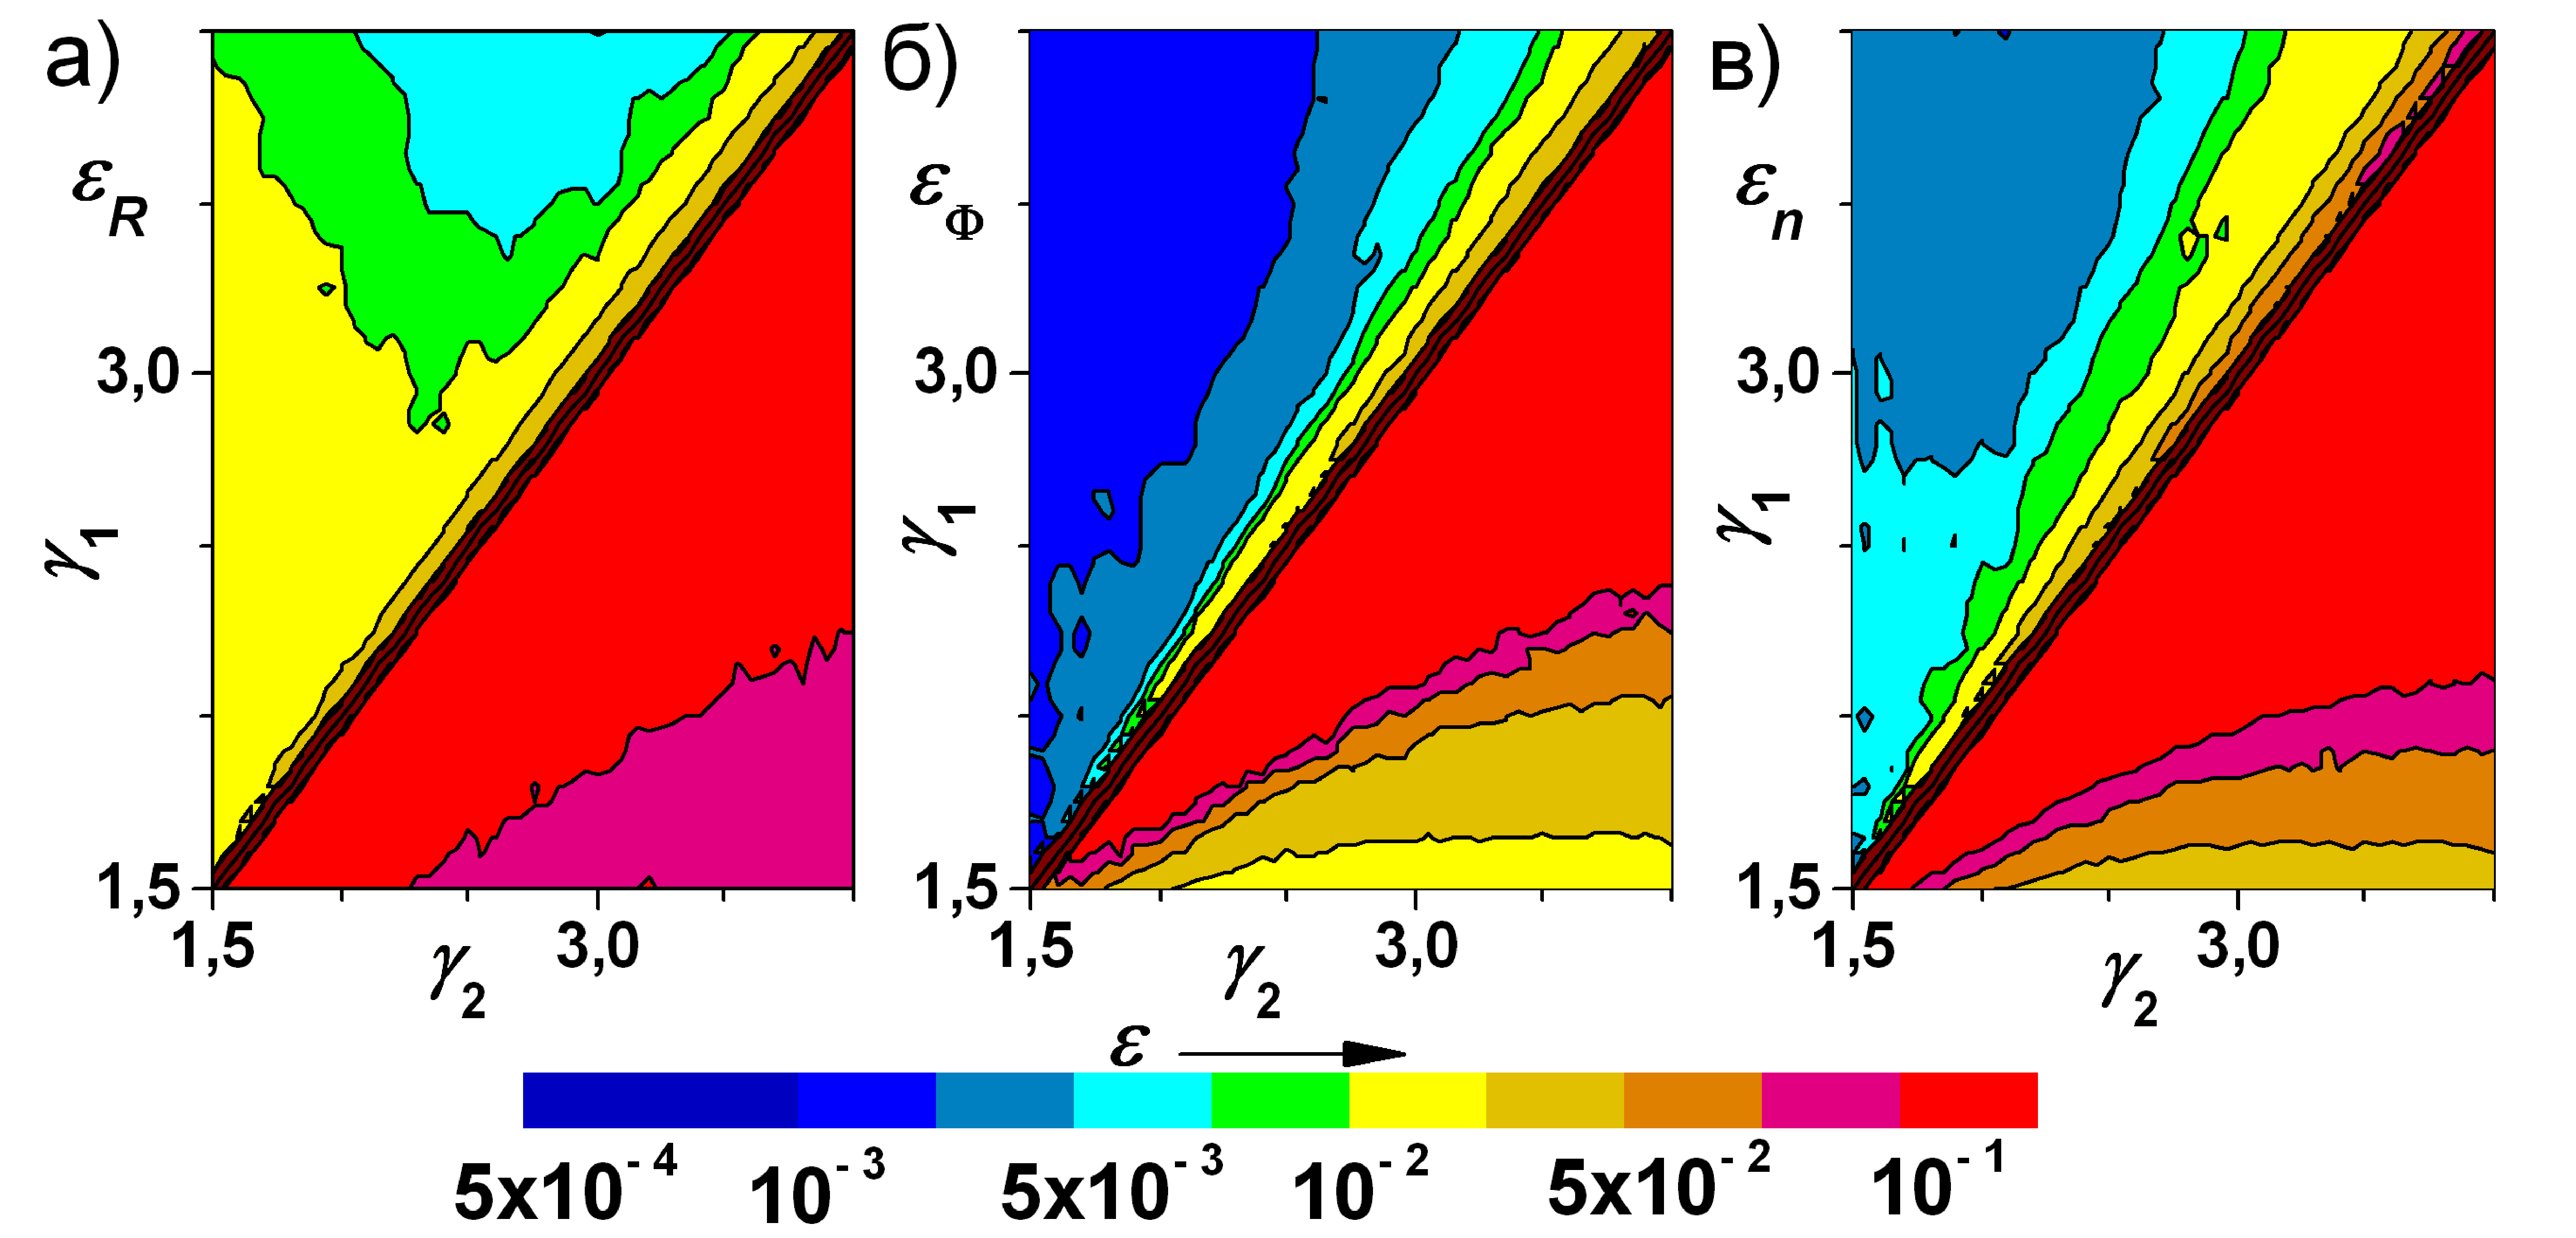
\includegraphics[width=0.8\textwidth]{figBohlin}%
\caption{\label{figBohlin}
Залежності похибок визначення $R_s$ (a), $\Phi_b$ (б) та $n_\mathrm{id}$ (в) від величини параметрів $\gamma_1$ та $\gamma_2$ при застосуванні метода Бохліна.
Наведено результати, отримані для наборів ідеальних ($\sigma_V=0$~V, $\sigma_I^\varepsilon=0$) синтезованих ВАХ (область $\gamma_1>\gamma_2$) та зашумлених ($\sigma_V=0,3$~мВ, $\sigma_I^\varepsilon=1\%$) даних (область $\gamma_2>\gamma_1$).
}
\end{figure}

В роботі \cite{Lee} для визначення параметрів ДШ запропоновано використовувати масив функцій $\{F_L(I)\}$:
\begin{equation}
\label{eqLee}
F_L(I)=V(I)-V_a\ln I,
\end{equation}
де
$V_a$ --- це довільне значення напруги.
Кожна з функцій $F_L(I)$ має бути апроксимована залежністю
\begin{equation}
\label{eqGrFit}
y(I)=c_1+c_2I+c_3\ln I
\end{equation}
та параметри $c_1$, $c_2$ та $c_3$ мають бути визначені.
Тоді очікується \cite{Lee}, що при $V>3kT/q$,
залежність $I_a=-c_3/c_2$ від $V_a$ має бути лінійною:
\begin{equation}
\label{eqLeeDet}
I_a(V_a)=(-n_\mathrm{id}kT/q+V_a)/R_s,
\end{equation}
що дозволяє визначити послідовний опір та фактор неідеальності.
В свою чергу, $\Phi_b$ може бути розрахований \cite{Lee} за допомогою виразу
\begin{equation}
\label{eqLeeFb}
\Phi_b=c_3/n_\mathrm{id}+kT/q\cdot\ln\left(AA^*T^2\right).
\end{equation}

В роботі при застосуванні даного методу використовувалися значення $V_a$ починаючи з 40~мВ з кроком 20~мВ;
апроксимація $F_L(I)$ здійснювалась за методом найменших квадратів.
Отримані дані позначені міткою <<Lee>>.

В роботі Д.~Громова та В.~Пугачевича \cite{Gromov} розглянуто два можливі шляхи визначення параметрів ДШ.
Згідно з першим з них, залежність напруги від струму може бути апроксимована виразом (\ref{eqGrFit}) причому
\begin{eqnarray}
\label{eqGr1}
R_s&=&c_2\,,
\\
n_\mathrm{id}&=&(c_3q)/(kT)\,,
\\
\Phi_b&=&\left[c_1/c_3+\ln\left(AA^*T^2\right)\right]kT/q\,.
\end{eqnarray}
Другий шлях полягає у тому, що вираз (\ref{eqGrFit}) застосовується до апроксимації функції Норда з $\gamma_N=2$:
\begin{equation}
\label{eqGr2}
F(I)=V(I)/2-kT/q\cdot\ln(I/AA^*T^2).
\end{equation}
В цьому випадку \cite{Gromov}
\begin{eqnarray}
\label{eqGr2Det}
R_s&=&2c_2\,,
\\
n_\mathrm{id}&=&(2c_3q)/(kT)+2\,,
\\
\Phi_b&=&\frac{2c_1}{n_\mathrm{id}}+\frac{(2-n_\mathrm{id})kT}{n_\mathrm{id}q}\ln\left(AA^*T^2\right)\,.
\end{eqnarray}
Застосування методів показало, що обидва підходи приводять до абсолютно однакових результатів.
Більше того, визначені значення параметрів дуже близькі до даних, які отримані за однакових початкових умов при використанні методу, описаного в роботі \cite{Lee} та згаданого трохи вище.
Тобто ці методи не є незалежними.

З іншого боку, проведені оцінки показали, що точність визначення параметрів за допомогою цих методів залежить від діапазону вихідної ВАХ, який використовується для побудови допоміжної функції, яка потім апроксимується залежністю (\ref{eqGrFit}).
Так, на Рис.~\ref{figGromov} наведено залежності похибок екстрагованих параметрів від початкового значення діапазону напруг, в якому проводилась апроксимація.
Видно, що для ідеальних ВАХ точність підвищується при звуженні використаного діапазону.
Водночас, для зашумлених даних спостерігається екстремальне значення точності  при певних значеннях ширини діапазону.
Причому ширина та положення діапазону, при якому точність визначення параметрів найбільша, залежить від рівня шуму.



\begin{figure}
\center
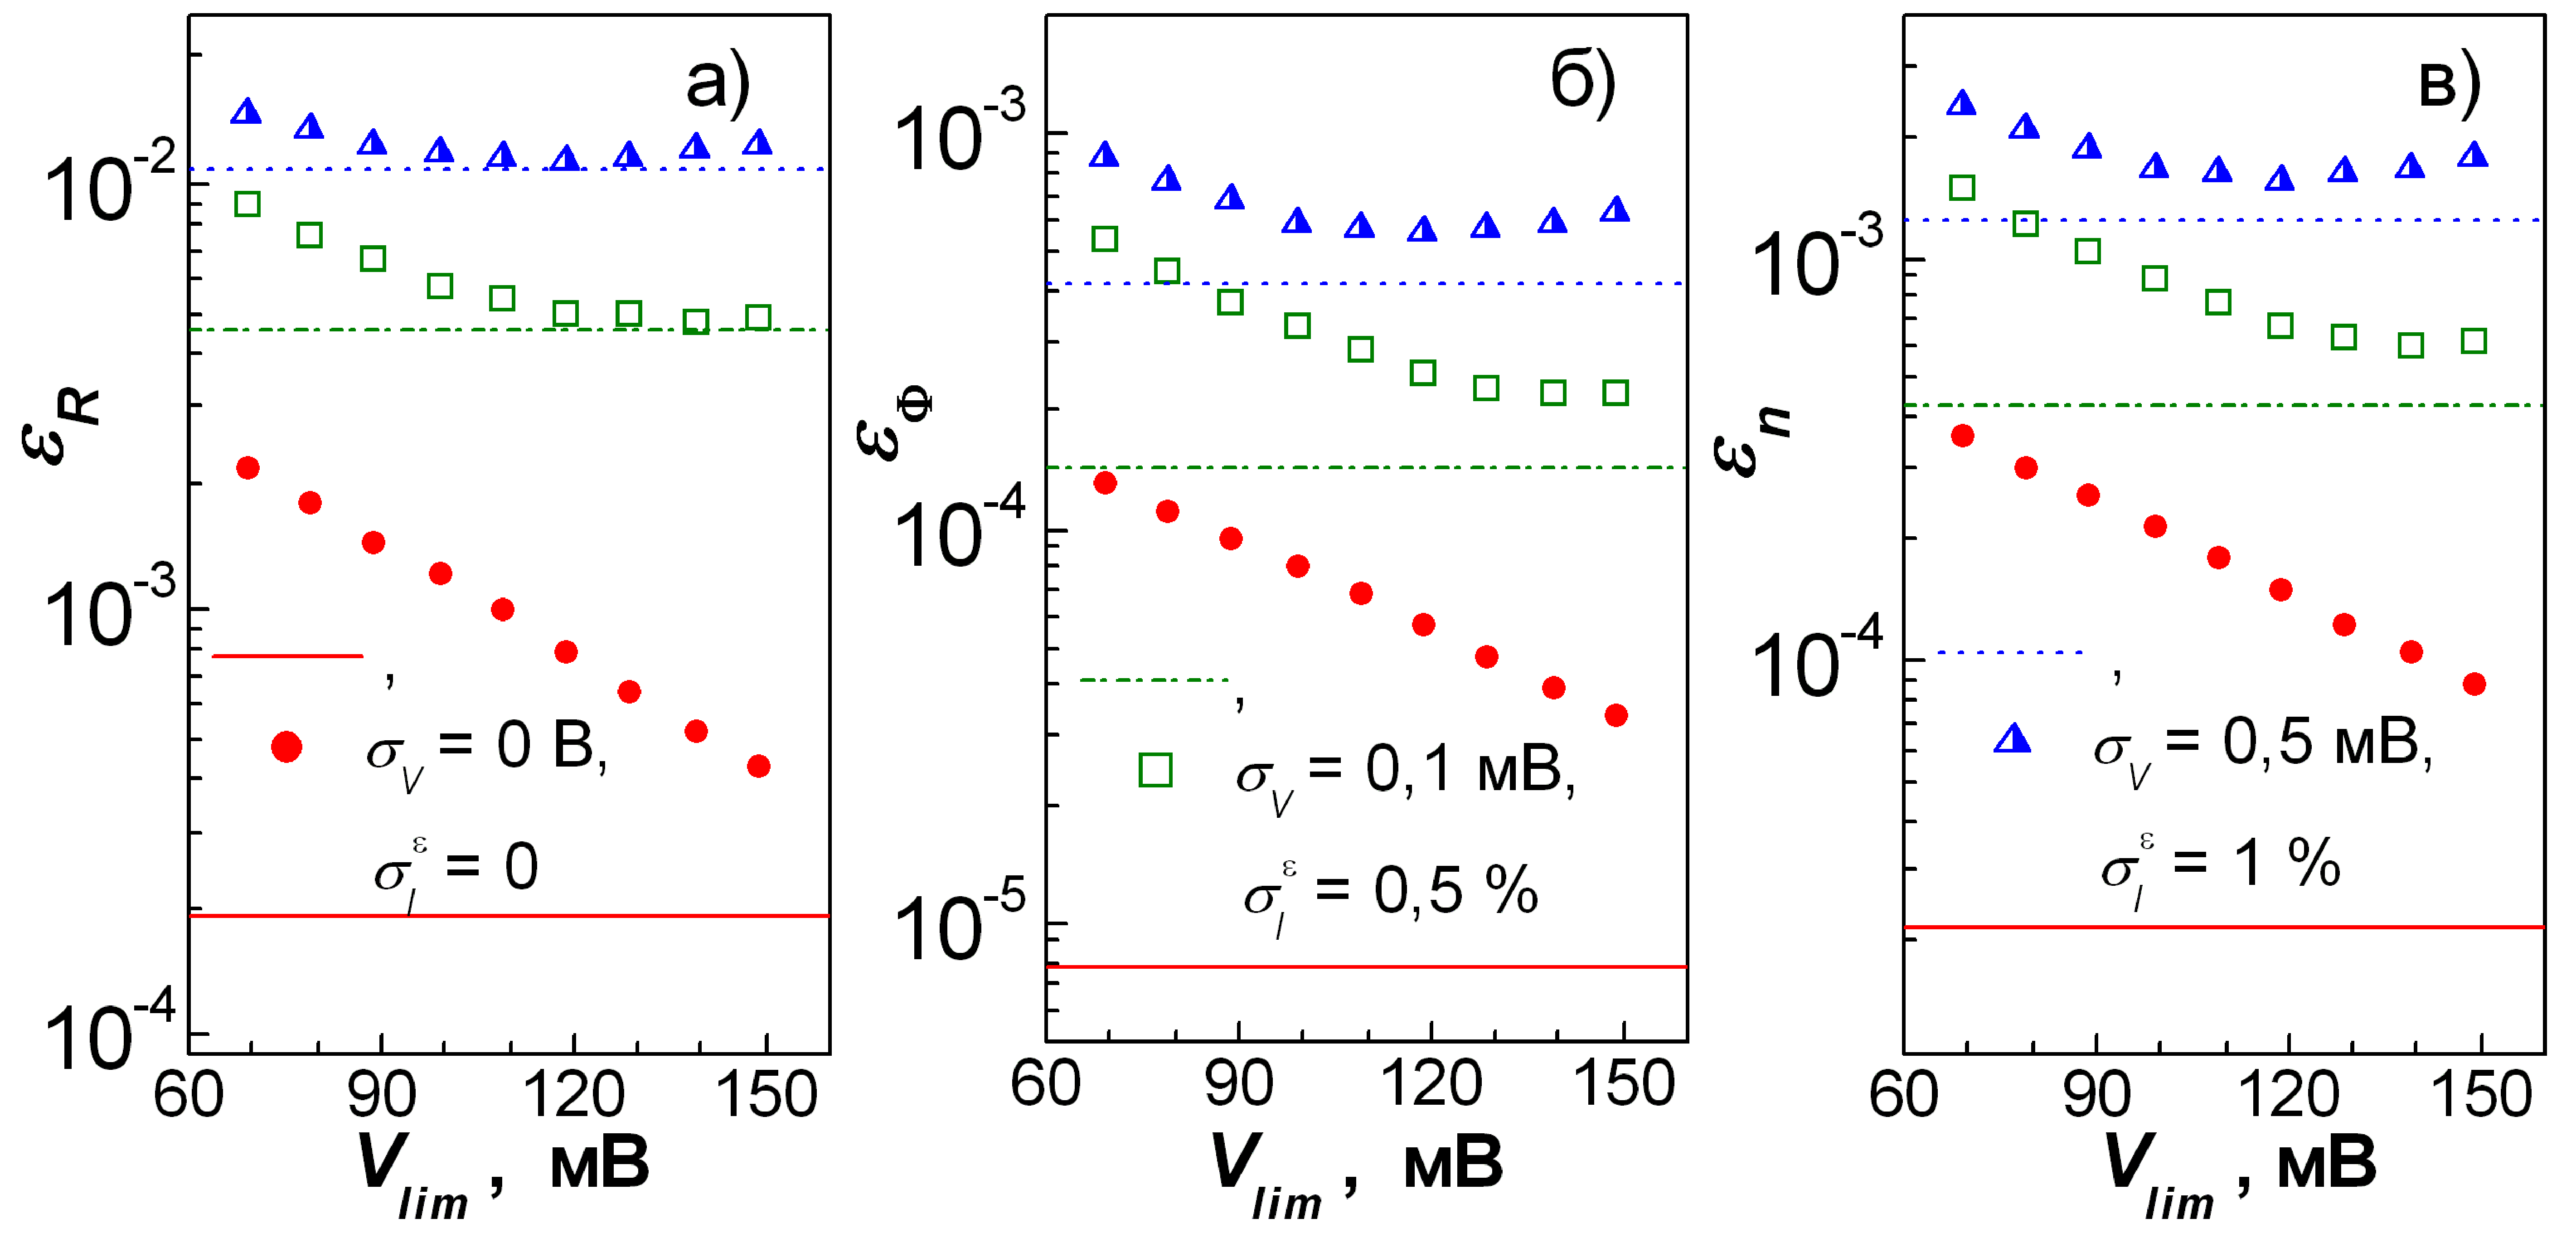
\includegraphics[width=0.9\textwidth]{figGromov}%
\caption{\label{figGromov}
Залежності похибок визначення $R_s$ (a), $\Phi_b$ (б) та $n_\mathrm{id}$ (в) при використанні методу Громова.
Наведено результати, отримані при апроксимуванні залежністю (\ref{eqGrFit}) допоміжної функції, побудованої
на основі ділянки ВАХ в діапазоні напруг від $V_{lim}$ до максимально значення.
Горизонтальні лінії вказують похибки значень параметрів ДШ, які отримані при використанні адаптивної процедури (див. текст).
Представлені результати, отримані при застосуванні методу до ідеальних синтезованих ВАХ (заповнені кружечки, суцільні лінії) та зашумлених даних
з $\sigma_V=0,1$~мВ та $\sigma_I^\varepsilon=0,5\%$ (незаповлені квадрати, штрих--пунктирні лінії) та з $\sigma_V=0,5$~мВ та $\sigma_I^\varepsilon=1\%$
(напівзаповнені трикутники, пунктирні лінії)
}
\end{figure}

У зв'язку з цим, для покращення ефективності роботи методів Громова та Лі, пропонується використовувати спеціальну адаптивну процедуру вибору діапазону побудови допоміжної функції.
Вона полягає в тому, що параметрів визначаються для всіх можливих діапазонів, кількість яких залежить від кількості точок вихідної ВАХ.
Після цього для кожного отриманого набору параметрів обчислюється величина $\theta=\sum_{i=1}^{N_p}[1-I_{calc}(V_i)/I_i]^2$,
де $I_{calc}(V_i)$ розраховується з використанням виразів (\ref{eqSDIV}) та (\ref{eqSDIs}).
Найкращим за точністю вважається той набір параметрів, для якого спостерігається мінімум величини $\theta$.

Зрозуміло, що подібна адаптивна процедура збільшує час, необхідних для визначення параметрів ДШ через необхідність багатократного повторення застосування методу Громова (Лі) та додаткових розрахунків.
Проте, з іншого боку, ця процедура може бути автоматизована, а також дозволяє підвищити точність --- див. лінії на Рис.~\ref{figGromov}.

Нижче представлені результати застосування методу Громова з використанням запропонованої адаптивної процедури.
Отримані дані позначені міткою <<Gromov>>.
Різниця між ними та позначеними міткою <<Lee>> визначає, фактично, доцільність запропонованої процедури.

В роботі \cite{Cheung} запропоновано визначати параметри ДШ шляхом побудови залежностей функцій $H(V)$
\begin{equation}
\label{eqH}
H(I)=V-\frac{n_\mathrm{id}kT}{q}\ln\left(\frac{I}{AA^*T^2}\right).
\end{equation}
та $dV/d(\ln I)$ від сили струму.
За умови $V_d>3kT/q$ ці залежності мають бути лінійними, причому
\begin{eqnarray}
\label{eqChung}
\frac{dV}{d\ln I}&=&R_sI+n_\mathrm{id}kT/q,
\\
\label{eqHDet}
H(I)&=&n_\mathrm{id}\Phi_b+IR_s.
\end{eqnarray}
При застосуванні методу спочатку визначаються $R_s$ та  $n_\mathrm{id}$ на основі рівняння (\ref{eqChung}),
а потім  $\Phi_b$, використовуючи вираз~(\ref{eqHDet}) та обчислене на попередньому кроці значення $n_\mathrm{id}$.
Отримані результати позначені міткою <<Chung>>.

Ще одним методом, де використовуються диференційні коефіцієнти ВАХ, є запропонований в роботі \cite{Mikhelashvili}.
В цьому випадку все починається з обчислення функції  $\alpha(V)$:
\begin{equation}
\label{eqMikh}
\alpha(V)=d(\ln I)/d(\ln V).
\end{equation}
Визначення параметрів відбувається з використанням співвідношень
\begin{eqnarray}
\label{eqMikhDet}
R_s&=&\frac{V_{max}}{\alpha^2_{max}I_{max}}\,,
\\
n_\mathrm{id}&=&\frac{qV_{max}(\alpha_{max}-1)}{\alpha_{max}^2kT}\,,
\\
\Phi_b&=&\frac{kT}{q}\left[\alpha_{max}+1-\ln\left(\frac{I_{max}}{AA^*T^2}\right)\right]\,.\label{eqMikhDetFi}
\end{eqnarray}
де
$\alpha_{max}$ та $V_{max}$  це координати максимуму залежності $\alpha$ від $V$;
$I_{max}$ --- сила струму, яка відповідає напрузі $V_{max}$.

\begin{figure}
\center
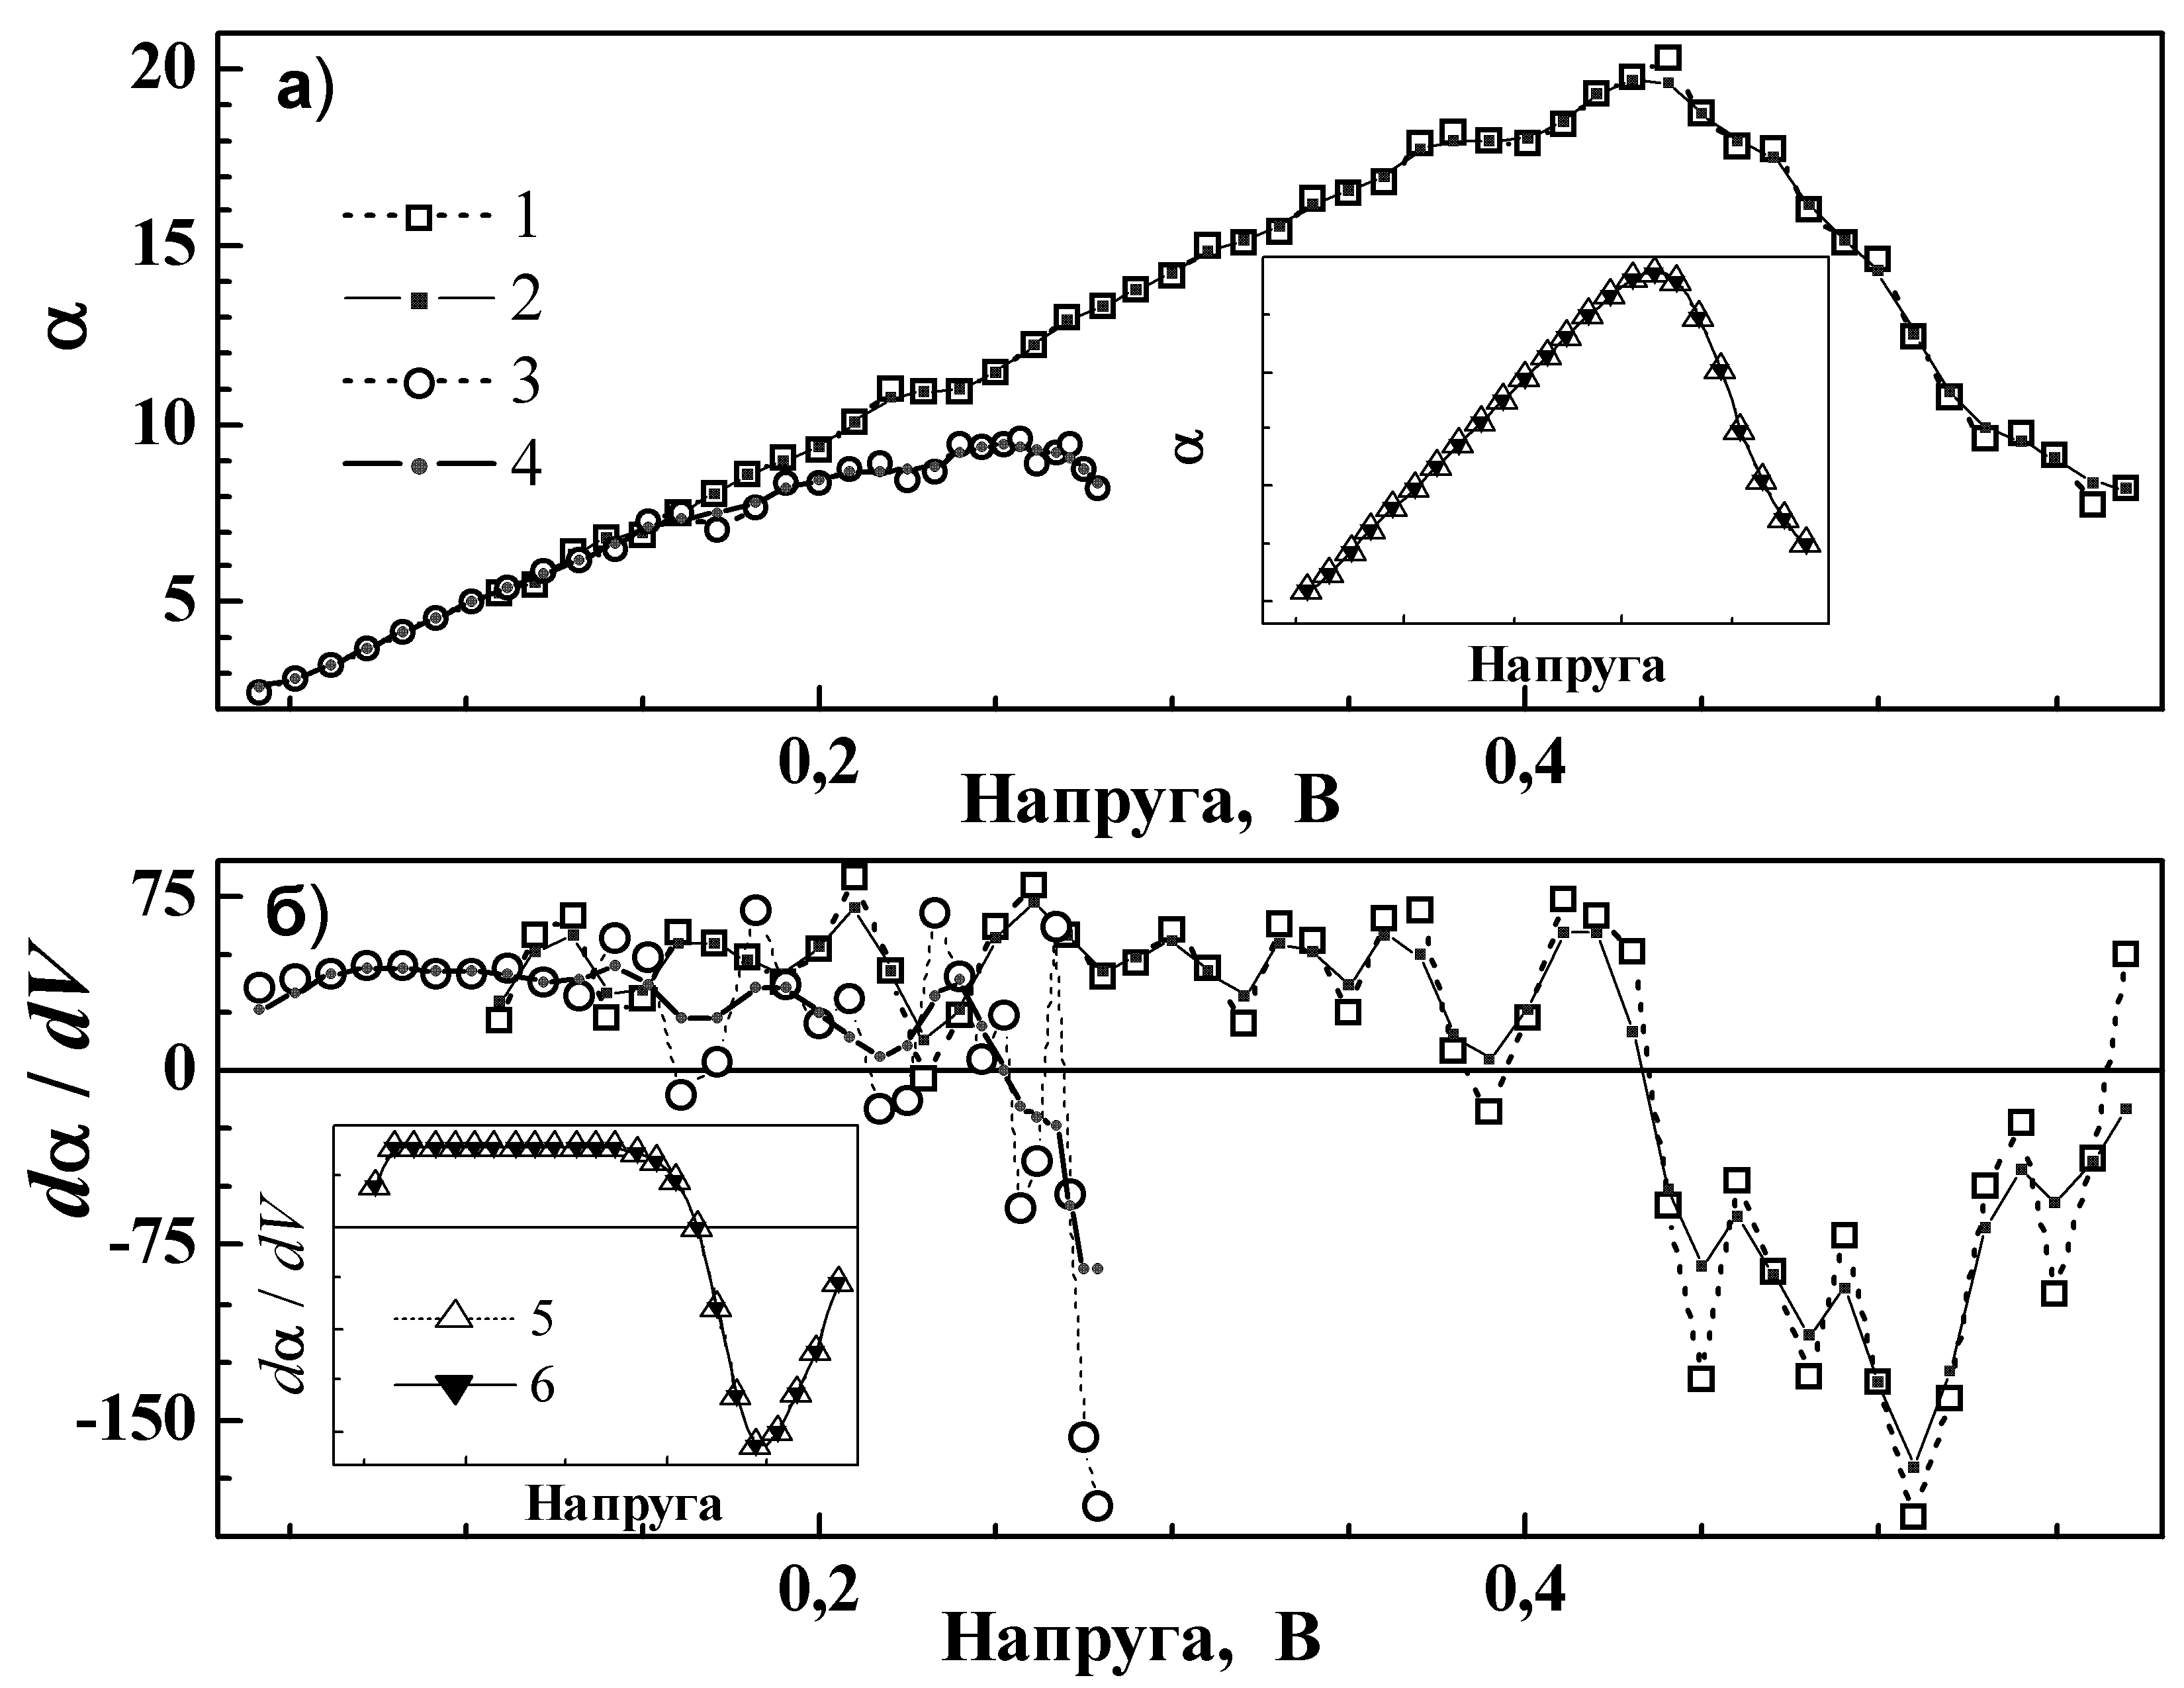
\includegraphics[width=0.65\textwidth]{figMikh}%
\caption{\label{figMikh}
Залежності функції~(\ref{eqMikh}) (а) та її похідної (б) від напруги.
Наведено графіки для зашумлених даних ($\sigma_V=0,3$~мВ, $\sigma_I^\varepsilon=1\%$, криві 1 та 2), для експериментально виміряних ВАХ (криві 3 та 4) та для ідеальних синтезованих ВАХ (вставка, криві 5 та 6) до (1, 3, 5) та після (2, 4, 6) запропонованої обробки.
}
\end{figure}

Зауважимо, що однією з необхідних властивостей методу, які використовуються для обчислення параметрів пристроїв з набору ВАХ, отриманих за різних умов, є можливість його застосування в автоматичному режимі.
В цьому випадку один з найпоширеніших варіантів пошуку екстремуму полягає у знаходженні нулів похідної.
Як видно з виразів (\ref{eqMikh})--(\ref{eqMikhDetFi}), для даного методу це означає необхідність проведення процедури чисельного знаходження другої похідної ВАХ.


Рис.~\ref{figMikh}(a) показує, що при використанні експериментальних ВАХ чи зашумлених даних чисельне диференціювання викликає появу багаточисленних локальних екстремумів на залежності функції $\alpha$ від $V$.
Ці екстремуми заважають автоматичному виявленню точки максимуму через наявність багатьох нульових точок на залежності $d\alpha/dV$ від $V$ --- див. Рис.~\ref{figMikh}(б).
З метою подолання цих труднощів, в роботі запропоновано проводити спеціальну 2-стадійну процедуру обробки даних.
А саме, на першій стадії обробки до отриманої з ВАХ залежності $\alpha$ від $V$ пропонується застосовувати 3--точковий медіанний фільтр, після чого, на другій стадії, проводити згладжування.
І лише після цього, проводити визначення положення максимуму, знаходження величин $\alpha_{max}$, $V_{max}$  та $I_{max}$ і розрахунок величин параметрів ДШ.
Дані на Рис.~\ref{figMikh} показують, що запропонована процедура обробки дійсно зменшує вплив побічних максимумів та дозволяє покращити точність методу.
Згладжування здійснюється завдяки усередненню по трьом сусіднім точкам з ваговими коефіцієнтами, які визначаються розподілом Гауса з дисперсією, рівною 0,6.

Надалі наведено результати, позначені міткою <<Mikhelashvili>> та отримані з використанням зазначеної процедури обробки.


\subsection{Чисельні методи}
Надалі також наведені результати отримані при використанні стандартного методу найменших квадратів зі статистичними ваговими коефіцієнтами \cite[с.~67]{KalitkinBook}.
В цьому випадку параметри визначались шляхом мінімізації квадратичної форми
\begin{equation}
\label{eqLS}
S(I_s,n_\mathrm{id},R_s)=\sum_{i=1}^{N_p}I_i^{-1}\left[I_i-I_{calc}(V_i,I_s,n_\mathrm{id},R_s)\right]^2,
\end{equation}
де $I_{calc}$ --- значення сили струму, отримане при інтерполяції.
При мінімізації шукався розв'язок системи рівнянь, отриманих з умов $\partial S/\partial I_s=0$,
$\partial S/\partial n_\mathrm{id}=0$ та $\partial S/\partial R_s=0$.
Пошук розв'язку цієї системи нелінійних рівнянь проводився за допомогою методу покоординаткого градієнтного спуску \cite[с.~231]{KalitkinBook}.
Як критерій зупинки ітераційного процесу було вибрано умову $\mid(S_j-S_{j+1})/S_j\mid<10^{-12}$,
де $S_j$ --- це значення квадратичної форми на $j-$му кроці ітерації.
Початкове наближення величини $R_s$ обчислювалося шляхом визначення перетину з координатною віссю залежності $(dV/dI)/I$ від $1/I$,
побудованої з використанням останніх п'яти точок ВАХ.
Початкові наближення $I_s$ та $n_\mathrm{id}$ отримувалися шляхом лінійної апроксимації залежності $\ln I$ від $V_d$, причому для визначення останньої величини використовувалися початкове наближення  $R_s$.

Було розглянуто два варіанти методу найменших квадратів.
В першому з них для обчислення $I_{calc}$ використовувався вираз ~(\ref{eqSDIV}), тобто квадратична форма мала вигляд
\begin{equation}
\label{eqLSOrd}
S(I_s,n_\mathrm{id},R_s)=\sum_{i=1}^{N_p}I_i^{-1}\left[I_i-I_s\left\{\exp\left[\frac{q(V_i-I_iR_s)}{n_\mathrm{id}kT}\right]-1\right\}\right]^2.
\end{equation}
Отримані внаслідок мінімізації функції~(\ref{eqLSOrd}) результати позначені міткою <<Ordinary LS>>.

В другому випадку при побудові квадратичної форми використовувалася $W$--функція Ламберта.
За визначенням, функція $W$ є розв'язком рівняння $z=W(z)\cdot\exp(W(z))$, її значення обчислюються за допомогою ряду \cite{LambertBook}.
Згідно з результатами, представленими в роботі \cite{Lambert_Jung}, явний розв'язок  трансцендентного рівняння~(\ref{eqSDIV}) може бути виражений за допомогою основної гілки функції Ламберта, причому у випадку нехтування впливом шунтуючого опору він має вигляд
\begin{equation}
\label{eqLam}
    I(V)=\frac{n_\mathrm{id}kT}{qR_s}W\left\{\frac{qR_s}{n_\mathrm{id}kT}
      \exp\left[\frac{q(V+R_sI_s)}{n_\mathrm{id}kT}\right]  \right\}+I_s.
\end{equation}
Тобто, квадратична форма може бути записана у вигляді
\begin{equation}
\label{eqLSLamb}
S(I_s,n_\mathrm{id},R_s)=\sum_{i=1}^{N_p}I_i^{-1}\left[I_i-\frac{n_\mathrm{id}kT}{qR_s}W\left\{\frac{qR_s}{n_\mathrm{id}kT}
      \exp\left[\frac{q(V_i+R_sI_s)}{n_\mathrm{id}kT}\right]  \right\}-I_s\right]^2,
\end{equation}
Результати, отримані при мінімізації (\ref{eqLSLamb}), позначені міткою <<Lambert LS>>.


\subsection{Еволюційні алгоритми\label{subEA}}
Еволюційні алгоритми -- це клас обчислювальних оптимізаційних моделей, які при своїй побудові та реалізації імітують поведінку живої природи.
При своїй роботі вони оперують наборами (популяціями) $P$ можливих розв'зків
$\overrightarrow{X}$: $P=\left\{\overrightarrow{X_k}\right\}$, $k\in(1,\ldots, N_S)$,
де $N_S$ --- це загальна кількість розв'язків у популяції.
Кожен із розв'язків (претендентів на звання остаточного розв'язку) є вектором, що складається з дійсних чисел:
$\overrightarrow{X_k}=\left\{x_{k,i}\right\}$, $i\in(1,\ldots, N_D)$,
де
$N_D$ дорівнює загальній кількості параметрів, які потрібно оптимізувати.
В нашому випадку $N_D=3$, $\overrightarrow{X}=\left\{R_s\,,\,n_\mathrm{id}\,,\,\ln I_s\right\}$.

Перед початком оптимізаційного процесу створюється початкова популяція.
Зазвичай початкові значення параметрів вибираються випадковим чином з інтервалу
$[\overrightarrow{X}^{L}, \overrightarrow{X}^{H}]$:
\begin{equation}
\label{eqEAIn}
x_{k,i,0}=x_i^L+r_{[0,1]}(x_i^H-x_i^L),
\end{equation}
де
$r_{[0,1]}$ --- випадкове число, рівномірно розподілене на інтервалі $[0,1]$,
$\overrightarrow{X}^{L}=\left\{x_i^L\right\}$ та $\overrightarrow{X}^{H}=\left\{x_i^H\right\}$ ---
нижня та верхня границі простору, де шукаються розв'язки, відповідно.
В даній роботі проводився пошук у просторі, границі якого задані наступним чином:
$R_s\in[0,\,50]$~Ом, $n_\mathrm{id}\in[1,\,2]$, $I_s\in[10^{-26},\,10^{-2}]$~A.

На кожному кроці ітерації
а)~проводиться трансформація кожного з розв'язків:
$\left\{\overrightarrow{X_{k}}_{,j-1}\right\}\rightarrow\left\{\overrightarrow{X_{k}}_{,j}\right\}$,
$j\in(1,\ldots, N_{it})$,
$N_{it}$ --- максимальна кількість ітерацій;
процедура трансформації залежить від конкретного алгоритму і описана далі;
б)~розраховується значення функції придатності (або цільової функції) $Fit(\overrightarrow{X_k}_{,j})$
для кожного $k$--го розв'язку.
Оптимальним для $j$--го ітераційного кроку розв'язком $\overrightarrow{X}_{j}^{opt}$ вважається той, для якого
значення функції придатності мінімальне:
$Fit(\overrightarrow{X}_{j}^{opt})=min\left\{Fit(\overrightarrow{X_k}_{,j})\right\}$.
Кінцевим результатом вважається $\overrightarrow{X}_{N_{it}}^{opt}$.

В даній роботі використовувалася цільова функція у вигляді суми квадратів відносних похибок апроксимації кожної з точок ВАХ
\begin{equation}
\label{eqEAFit}
Fit=\sum_{i=1}^{N_p}\left\{1-\frac{I_s}{I_i}\left[\exp\left(\frac{q(V_i-I_iR_s)}{nkT}\right)-1\right]\right\}^2.
\end{equation}
$N_{it}$ визначалося умовою збіжності розв'язку.

Метод диференційної еволюції імітує процеси природного відбору і використовує процеси диференційної мутації та випадкового схрещування.
У термінології даного алгоритму кожен з розв'язків називається особою, а послідовність дій на $j$--му ітераційному кроці має наступний вигляд \cite{DEWang,DEModif}:
\begin{itemize}[leftmargin=0cm,itemindent=1em]
  \item Мутація. Для кожного вектору $\overrightarrow{X_{k}}_{,j-1}$ генерується вектор мутації $\overrightarrow{M_{k}}_{,j}$
  \begin{equation}
 \label{eqDEMut}
 \overrightarrow{M_{k}}_{,j}=\overrightarrow{X_{r_1}}_{,j-1}+F_{sc}\cdot\left(\overrightarrow{X_{r_2}}_{,j-1}-\overrightarrow{X_{r_3}}_{,j-1}\right),
 \end{equation}
 де $r_1,r_2,r_3\in(1,\ldots,N_S)$ вибираються випадковим чином і мають відрізнятися від індексу $k$.
 $F_{sc}\in[0,2]$  --- дійсна стала величина, що називається масштабним коефіцієнтом.


  \item Схрещування. Формується пробний вектор $\overrightarrow{U_{k}}_{,j}$
  \begin{equation}
 \label{eqDECros}
 u_{k,i,j}=\left\{
 \begin{array}{ll}
 m_{k,i,j},& \text{if} \quad r_{[0,1]}\leq C\!R \quad \text{or} \quad i=r_{4}\\
 x_{k,i,j-1},& \text{otherwise}
 \end{array}
 \right.
 \end{equation}
 причому випадкова величина $r_4\in(1,\ldots,N_D)$
забезпечує наявність в $\overrightarrow{U_{k}}_{,j}$ хоча б одного елемента з $\overrightarrow{M_{k}}_{,j}$;
 константа $C\!R\in[0,1]$ називається темп схрещування.
  Спираючись на результати, представлені в \cite{P-DE_Ishaque},
  в даній роботі в даній роботі були використана штрафна функція, яка запобігає виходу розв'язків за межі пошукового простору.
  А саме, будь--який параметр, значення якого перевищувала допустимі межі, замінювався випадковою величиною згідно з
    \begin{equation}
 \label{eqDEPen}
 u_{k,i,j}=\left\{
 \begin{array}{ll}
 u_{k,i,j}-r_{[0,1]}(x_i^H-x_i^L),& \text{if} \quad u_{k,i,j}>x_i^H\\
 u_{k,i,j}+r_{[0,1]}(x_i^H-x_i^L),& \text{if} \quad u_{k,i,j}<x_i^L.
 \end{array}
 \right.
 \end{equation}
  \item Відбір.
      \begin{equation}
 \label{eqDESel}
 \overrightarrow{X_{k}}_{,j}=\left\{
 \begin{array}{ll}
\overrightarrow{U_{k}}_{,j},& \text{if} \quad Fit(\overrightarrow{U_k}_{,j})<Fit(\overrightarrow{X_k}_{,j-1})\\
 \overrightarrow{X_{k}}_{,j-1},& \text{otherwise}.
 \end{array}
 \right.
 \end{equation}

\end{itemize}
Користуючись результатами, представленими в \cite{DEWang},
були вибрані значення $F_{sc}=0,8$, $C\!R=0,3$ та $N_S=8N_D=24$.
Виявлено, що збіжність результатів досягається при $N_{it}=600$.
Отримані результати позначені міткою <<DE>>.

Розвиток методу оптимізації зграї частинок пов'язаний зі спостереженням соціальної поведінки тварин на кшталт зграї птахів чи риб.
У термінології алгоритму PSO розв'язки називаються частинками, які летять (чи плавають) і гіперпросторі параметрів.
На $j$--му ітераційному кроці виконуються наступні дії \cite{PSO_Ye}:
\begin{itemize}[leftmargin=0cm,itemindent=1em]
  \item Визначається найкраще положення $\overrightarrow{X_k}_{,j}^{best}$ для кожної з частинок:
 \begin{equation}
 \label{eqPSO_PB}
 \overrightarrow{X_k}_{,j}^{best}=\left\{
 \begin{array}{ll}
 \overrightarrow{X_k}_{,j-1}^{best},& \text{if} \quad Fit(\overrightarrow{X_k}_{,j-1})\geq Fit(\overrightarrow{X_k}_{,j-1}^{best})\\
 \overrightarrow{X_{k}}_{,j-1},& \text{otherwise}.
 \end{array}
 \right.
 \end{equation}
  \item  Визначається глобально найкраща позиція $\overrightarrow{B}_{j}$ серед всіх частинок зграї:
 \begin{equation}
 \label{eqPSO_GB}
 \overrightarrow{B}_{j}=min\{ Fit(\overrightarrow{X_1}_{,j}^{best}),\ldots, Fit(\overrightarrow{X_{N_S}}_{,j}^{best})\}.
 \end{equation}
  \item Змінюється вектор швидкості кожної частинки
\begin{eqnarray}
 \label{eqPSO_Vel}
\upsilon_{k,i,j}&=&w_j\,\upsilon_{k,i,j-1}+l_1r_{[0,1],1}\cdot(x_{k,i,j}^{best}-x_{k,i,j-1})+
\nonumber\\
&&l_2r_{[0,1],2}\cdot(b_{i,j}-x_{k,i,j-1})
\,,
\end{eqnarray}
де
$l_1$ та $l_2$ називаються коефіцієнти навчання, $w_j$ --- інерційна маса.
У даній роботі, використано підхід лінійного збільшення маси:
 \begin{equation}
 \label{eqPSO_W}
 w_j=w_{max}-j(w_{max}-w_{min})/N_{it},
 \end{equation}
де
$w_{max}$ та $w_{min}$ --- початкова та кінцева маси, відповідно.
Після цього швидкість кожної з частинок оновлюється з використанням наступного виразу:
 \begin{equation}
 \label{PSO_Vmax}
 \upsilon_{k,i,j}=\left\{
 \begin{array}{ll}
 \upsilon_{i}^{max},& \text{if} \quad \upsilon_{k,i,j}>\upsilon_{i}^{max}\\
 -\upsilon_{i}^{max},& \text{if} \quad \upsilon_{k,i,j}<-\upsilon_{i}^{max}\\
 \upsilon_{k,i,j},& \text{otherwise}\,,
 \end{array}
 \right.
 \end{equation}
де
константа $ \overrightarrow{\upsilon}^{max}$  призначена стримувати надлишкові блукання частинок.
Зазвичай \cite{PSO_Ye} $ \overrightarrow{\upsilon}^{max}$ вибирається рівним максимально можливому відхиленню даної частинки в певному напрямі.
 \item Кожна частинка переміщується у нове положення:
 \begin{equation}
 \label{eqPSO_Final}
 \overrightarrow{X_{k}}_{,j}=\overrightarrow{\upsilon_{k}}_{,j}+\overrightarrow{X_{k}}_{,j-1},
 \end{equation}
\end{itemize}
Згідно з \cite{PSO_Ye}, було використано наступні значення параметрів:
$l_1=l_2=2$, $w_{max}=0,9$, $w_{min}=0,4$ та $N_S=15N_D=45$.
Крім того, при розрахунках вважалося, що початкові швидкості $\overrightarrow{\upsilon_{k}}_{,0}=0$.
Виявлено, що збіжність результатів досягається при $N_{it}=700$.
Отримані результати позначені міткою <<PSO>>.

Алгоритм методу модифікованої штучної бджолиної сім'ї базується на поведінці рою медоносних бджіл, пов'язаній з пошуком їжі.
Бджоли поділяються на три категорії: носії, спостерігачі та розвідники.
Носії експлуатують свої джерела їжі та взаємодіють зі спостерігачами.
Спостерігачі очікують у вулику та вирішують яке з джерел їжі експлуатувати.
Розвідники проводять пошуки нових джерел їжі навколо вулика.
Кількість носіїв та спостерігачів збігається з кількістю розв'язків.
Самі розв'язки описують розташування джерел їжі, а кількість нектару в джерелі визначається придатністю розв'язку.
Коли джерело їжі повністю вичерпується, пов'язані з ним носії стають розвідниками.
Дії, які передбачені під час $j$--ої ітерації наступні \cite{MABC}:
\begin{itemize}[leftmargin=0cm,itemindent=1em]
  \item Створюється новий розв'язок $\overrightarrow{T_{k}}_{,j}$ для кожного носія
 \begin{equation}
 \label{eqMABCNew}
 \overrightarrow{T_{k}}_{,j}=\overrightarrow{X_{k}}_{,j-1}+r_{[-1,1]}(\overrightarrow{X_{k}}_{,j-1}-\overrightarrow{X_{r}}_{,j-1}),
 \end{equation}
 де
 $r\in(1,\ldots,N_S)$ --- це випадковим чином вибраний індекс, $r\neq k$.
  \item Застосовується жадібний процес відбору до носіїв:
 \begin{eqnarray}
 \label{eqMABC_GS1}
 \overrightarrow{X_{k}}_{,j-1}=\left\{
 \begin{array}{ll}
\overrightarrow{T_{k}}_{,j},& \text{if} \: Fit(\overrightarrow{T_k}_{,j})<Fit(\overrightarrow{X_k}_{,j-1})\\
 \overrightarrow{X_{k}}_{,j-1},& \text{otherwise}.
 \end{array}
 \right.
 \\
 \label{eqMABC_GS2}
 s_k=\left\{
 \begin{array}{ll}
0,& \text{if} \: Fit(\overrightarrow{T_k}_{,j})<Fit(\overrightarrow{X_k}_{,j-1})\\
s_k+1 ,& \text{otherwise}.
 \end{array}
 \right.
 \end{eqnarray}
 Тут $\overrightarrow{S}=\{s_1,\ldots,s_{N_S}\}$ вектор, який містить інформацію щодо зручності всіх джерел їжі.
 Початкові значення $s_k=0$.

 \item Розраховується ймовірність $p_k$ для кожного розв'язку:
 \begin{equation}
 \label{eqMABCP}
 p_k=\frac{(1+ Fit(\overrightarrow{X_k}_{,j-1}))^{-1}}{\sum_{m=1}^{N_S}(1+ Fit(\overrightarrow{X_m}_{,j-1}))^{-1}}.
  \end{equation}

 \item Для кожного спостерігача

 а)~створюється новий розв'язок $\overrightarrow{T_{k}}_{,j}$ з вибраного розв'язку
$\overrightarrow{X_{k}}_{,j-1}$ by using Eq.~(\ref{eqMABCNew}) if $r_{[0,1]}<p_k$, $k={1,\ldots,N_S}$;

 б)~застосовується механізм жадібного вибору --- див. рівняння~(\ref{eqMABC_GS1}) та (\ref{eqMABC_GS2}).

 \item
 Визначають відкинуті розв'язки та, відповідно, розвідники, і якщо вони існують, розв'язки замінюються новими, створеними випадковим чином
  \begin{equation}
 \label{eqMABCSC}
 x_{k,i,j}=\left\{
 \begin{array}{ll}
 x_i^L+r_{[0,1]}(x_i^H-x_i^L) & \text{if} \quad s_k>L_{imit}
 \\
 x_{k,i,j-1},& \text{otherwise}.
 \end{array}
 \right.
 \end{equation}
 де
 $L_{imit}$ --- регулюючий параметр алгоритму, який визначає допустиме число поколінь, протягом яких кожне джерело їжі має бути відкинуте.
\end{itemize}

В розрахунках були використані значення $L_{imit}=36$ та $N_S=24$ \cite{MABC}.
Крім того вважалося, що найкращий розв'язок не може біти відкинуто.
Виявлено, що збіжність результатів досягається при $N_{it}=250$.
Отримані результати позначені міткою <<MABC>>.

Алгоритм оптимізованого викладання та навчання використовує концепцію навчального процесу в класі.
Група учнів у класі розглядається як популяція розв'язків.
Алгоритм імітує процес навчання, при якому учні спочатку отримують знання від учителя, а потім також і внаслідок спілкування між собою.
На $j$--му кроці ітераційного процесу дії описуються наступним чином\cite{TLBO_Patel}:
\begin{itemize}[leftmargin=0cm,itemindent=1em]
  \item Етап учителя.
 Проводиться модифікація знань учня $\overrightarrow{T_{k}}_{,j}$ 
   \begin{equation}
  \label{eqTLBOTP}
   \overrightarrow{T_{k}}_{,j}=\overrightarrow{X_{k}}_{,j-1}+r_{[0,1]}\left(\overrightarrow{X}_{j-1}^{opt}-
      r_{(1,\ldots,2)}\overrightarrow{X}_{j-1}^{mean}\right),
  \end{equation}
  для кожної особи ($\overrightarrow{X_{k}}_{,j-1}$) в класі за виключенням вчителя ($\overrightarrow{X}_{j-1}^{opt}$).
  Тут
    \begin{equation}
 \label{eqTLBOMean}
  x_{i,j-1}^{mean}=\frac{1}{N_S}\sum_{k=1}^{N_S}x_{k,i,j-1}.
  \end{equation}
  Якщо $\overrightarrow{T_{k}}_{,j}$ є кращим ніж $\overrightarrow{X_{k}}_{,j-1}$, то він його замінює згідно з~(\ref{eqMABC_GS1}).



  \item Етап учня.
  Для кожного з учнів генерується новий розв'язок $\overrightarrow{U_{k}}_{,j}$, причому
\begin{eqnarray}
 \label{eqTLBOLP}
 \overrightarrow{U_{k}}_{,j}&=&\overrightarrow{X_{k}}_{,j-1}+r_{[0,1]}\left(\overrightarrow{X_{k}}_{,j-1}-\overrightarrow{X_{r}}_{,j-1}\right),
\\
&& \text{if}\quad Fit(\overrightarrow{X_{k}}_{,j-1})>Fit(\overrightarrow{X_{r}}_{,j-1})
\nonumber
\\
 \label{eqTLBOLP2}
 \overrightarrow{U_{k}}_{,j}&=&\overrightarrow{X_{k}}_{,j-1}-r_{[0,1]}\left(\overrightarrow{X_{k}}_{,j-1}-\overrightarrow{X_{r}}_{,j-1}\right),
\\
&& \text{if}\quad Fit(\overrightarrow{X_{k}}_{,j-1})\leq Fit(\overrightarrow{X_{r}}_{,j-1}),
\nonumber
\end{eqnarray}
де
$r\in(1,\ldots,N_S)$ --- індекс, вибраний випадковим чином, $r\neq k$.
Після цього використовується вираз~(\ref{eqDESel}) для визначення $\overrightarrow{X_{k}}_{,j}$.
\end{itemize}
В роботі використовувалася величина $N_S=1000$.
Розрахунки показали, що збіжність розв'язку спостерігається при $N_{it}=900$.
Отримані результати позначені міткою <<TLBO>>.

\section{Порівняння ефективності методів визначення параметрів структур метал--напівпровідник}

\subsection{Точність визначення параметрів на основі ідеальних ВАХ}

\begin{figure}
\center
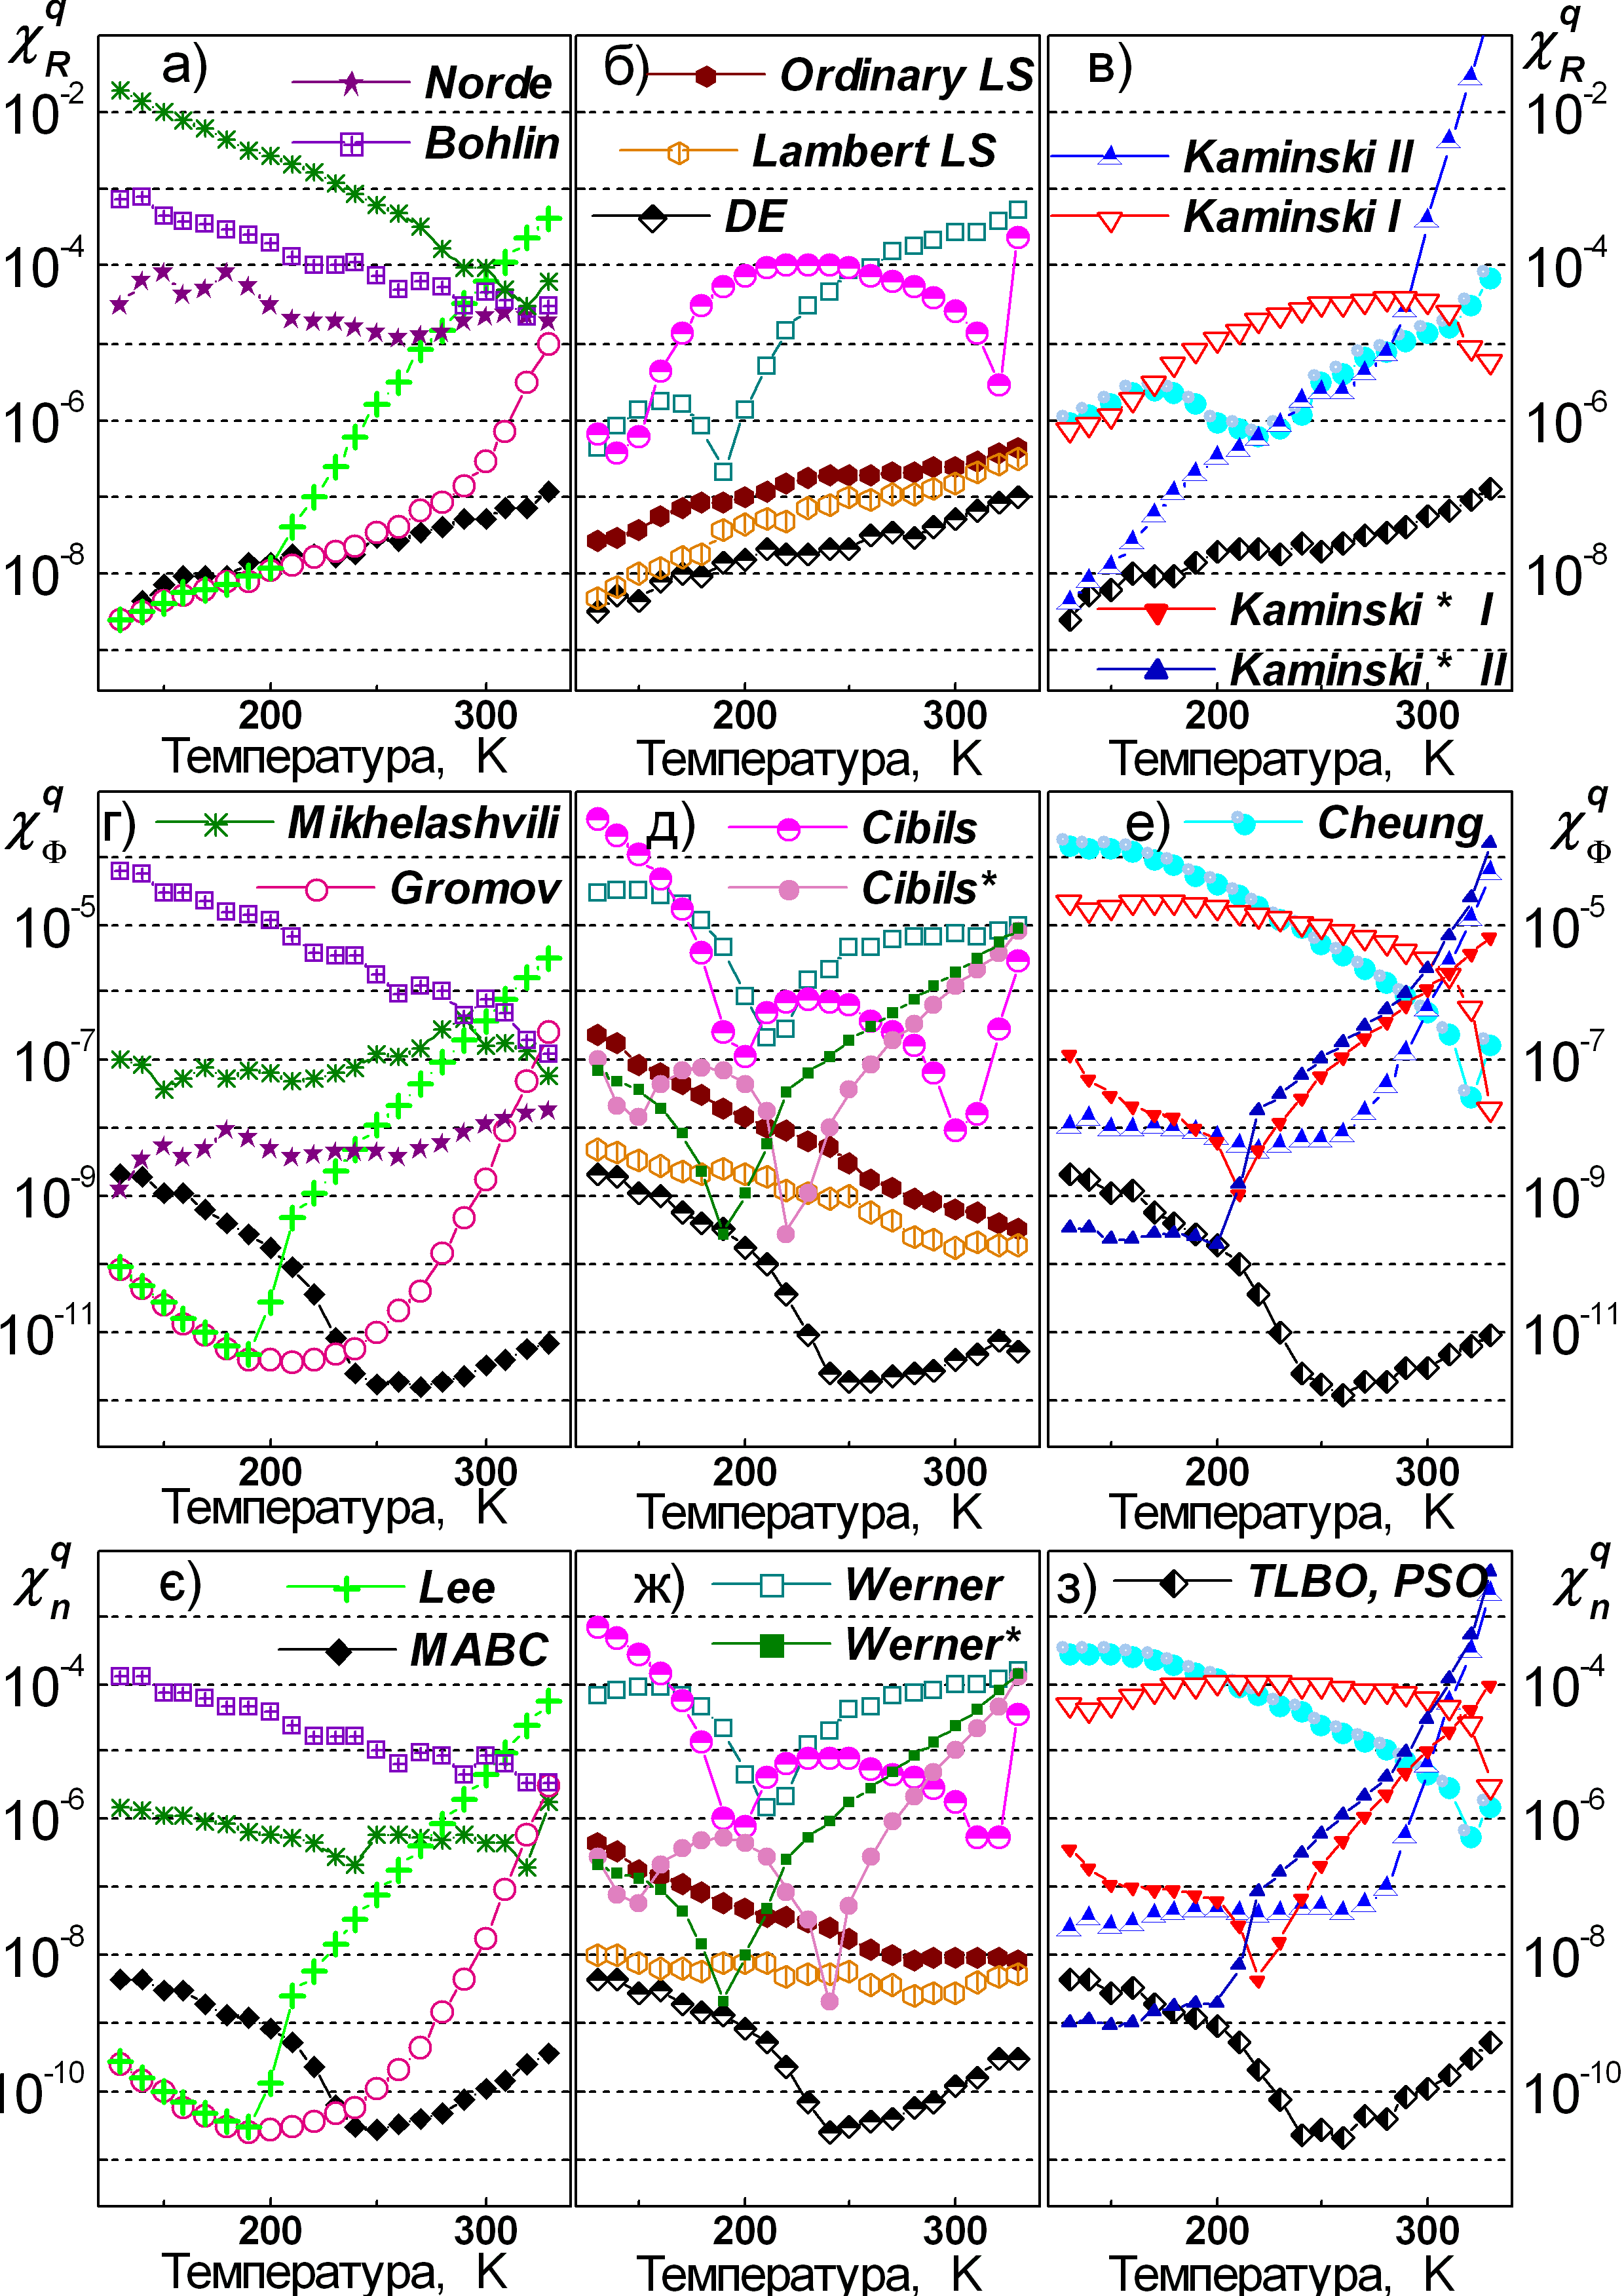
\includegraphics[width=0.85\textwidth]{figId}%
\caption{\label{figId}
Температурні залежності відносних похибок визначення $R_s$ (а --- в), $\Phi_b$ (г --- е) та $n_\mathrm{id}$ (є --- з) при застосуванні різних методів до ідеальних синтезованих ВАХ.
%Залежності точності визначення послідовного опору (а --- в), ВБШ (г --- е) та фактору неідеальності (є --- з) при використанні різних методів від температури.
%Результати отримані при використанні ідеальних синтезованих ВАХ.
}
\end{figure}

Точність визначення параметрів з окремої ВАХ залежно від температури, при якій її синтезовано, наведено на Рис.~\ref{figId}.
Насамперед зауважимо, що наведені дані показують:
\begin{enumerate}[label=\asbuk*),leftmargin=0em,itemindent=1.5em]
%\begin{enumerate}[label=\asbuk*),labelindent=0em,itemindent=1.5em]
\item при використанні всіх еволюційних алгоритмів для аналізу однакових ВАХ були отримані дуже близькі значення як послідовного опору, так і ВБШ та фактору неідеальності;
це цілком очікуваних результат, пов'язаний з тим що у всіх випадках використовувалася ідентична цільова функція;
\item використання адаптивної процедури в методі Gromov дає можливість суттєво знизити помилки визначення параметрів;
\item використання функції Ламберта при чисельних обчисленнях дозволяє зменшити помилки визначення параметрів порівняно з випадком, коли в методі найменших квадратів використовується трансцендентна форма рівняння ВАХ;
\item при застосуванні методів Werner, Cibils, та Kaminskii~I шляхом лінійної апроксимації допоміжної функції доцільно визначати лише величину послідовного опору,
тоді як $\Phi_b$ та $n_\mathrm{id}$ краще екстрагувати на наступному етапі, при лінійній апроксимацій ВАХ, скорегованої з врахуванням  отриманого значення $R_s$;
іншими словами використання варіантів цих методів, позначених зірочками дозволяє підвищити точність визначення параметрів;
\item найбільшу точність при аналізі ідеальних синтезованих ВАХ вдається досягти при використанні еволюційних алгоритмів, апроксимації за допомогою методу найменших квадратів з використанням функції Ламберта, Norde (при визначенні $\Phi_b$), Ordinary LS (при визначенні $R_s$), методу Gromov, доповненого адаптивною процедурою, та методу Lee (за винятком випадків високих температур та великих значень $I_s$).
\end{enumerate}




\begin{figure}
\center
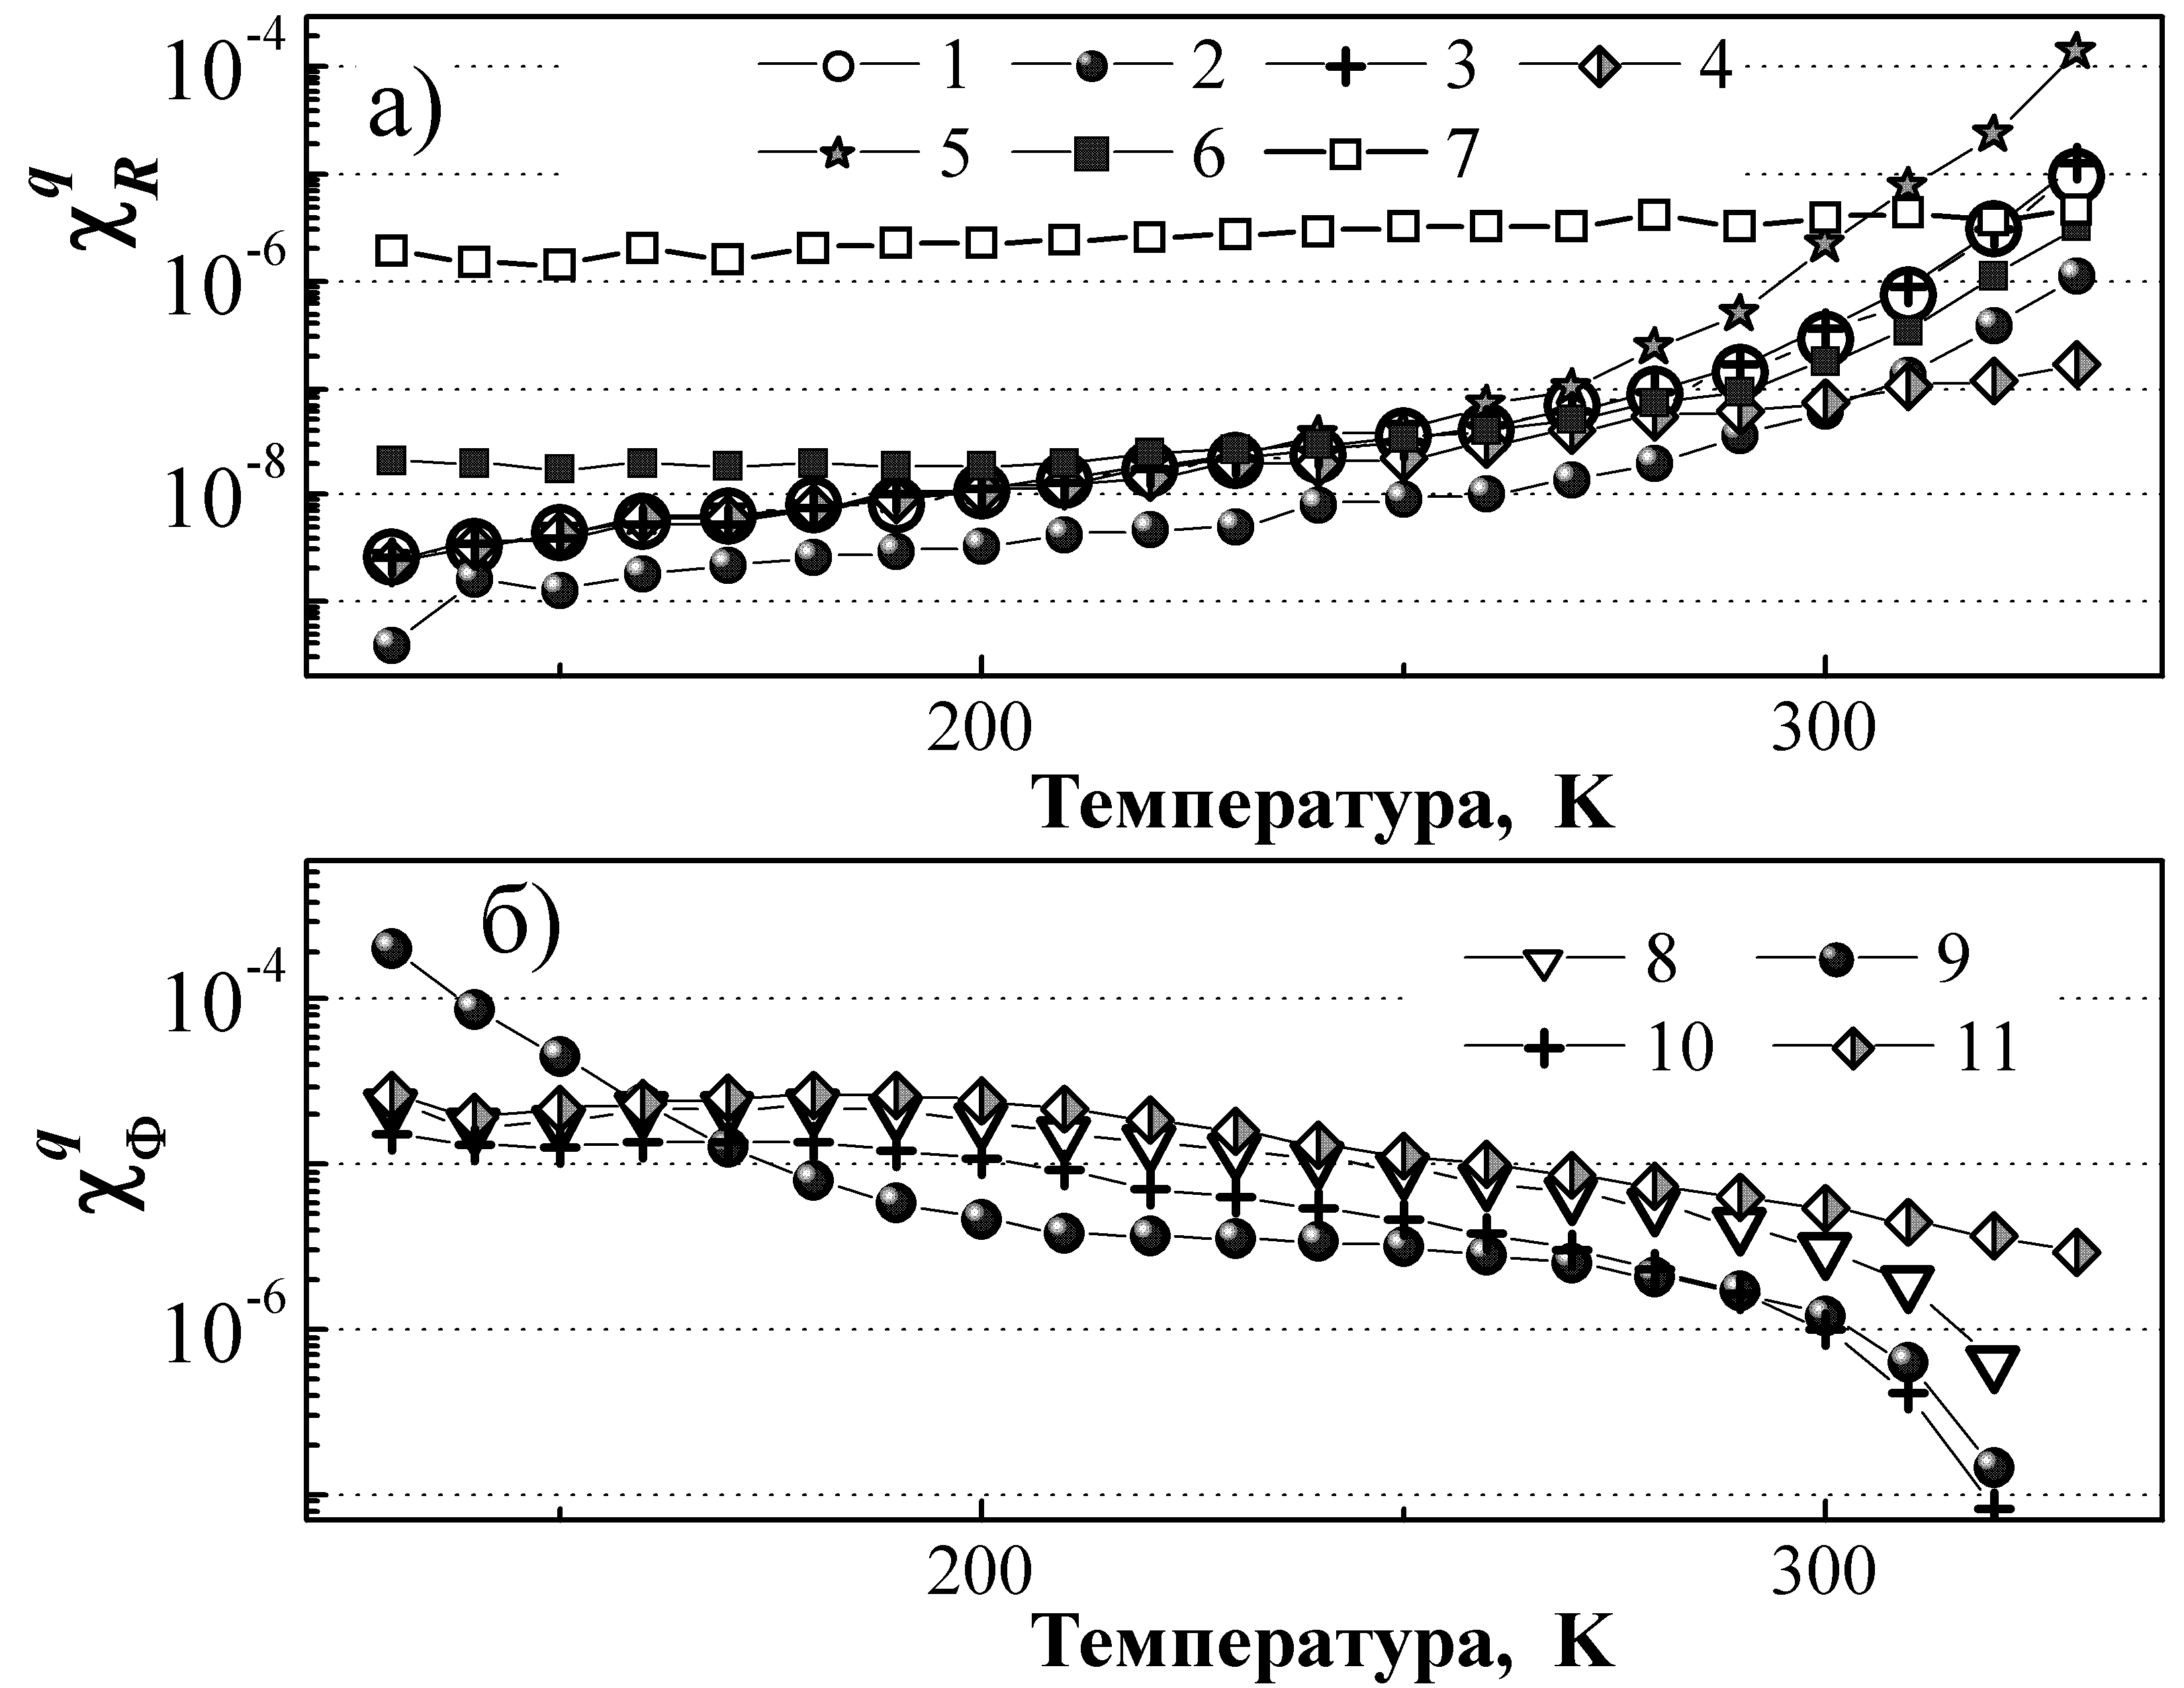
\includegraphics[width=0.65\textwidth]{figCon}%
\caption{\label{figCon}
Температурні залежності похибок визначення $R_s$ (a) та $\Phi_b$ (б) при використанні методів Gromov (a) та  Kaminskii I (б).
Під час синтезу ВАХ використовувалися параметри, величини яких переважно визначались формулами~(\ref{eqSDIs}--\ref{eqRsT}),
проте для  побудови кривих 2 та 9 використовувалися ВАХ для яких значення $R_s$ було в 3 рази більше,
для кривих 3 та 10 величина $n_\mathrm{id}$ була в 1,2 рази більша,
для кривих 4 та 11 величина $I_s$ була в 100 разів менша,
для кривої 5 значення $\Phi_b$ було зменшено на 0,1 еВ,
для кривої 6 величини $R_s$ та $\Phi_b$ залишалися незмінними та рівними 2~Ом та 0,7~еВ, відповідно, під час синтезу всього
набору ВАХ (були незалежні від температури),
для кривої 7 значення $R_s$ та $I_s$ були незмінні та рівні 2~Ом та $10^{-5}$~A, відповідно.
}
\end{figure}

З іншого боку, наведені результати показують, що точність визначення параметрів змінюється для різних ВАХ з одного набору (залежить від температури, при якій ВАХ була синтезована).
Фактично мова йде про те, що похибка визначення параметру з масиву $\left\{R_s\,,\,n_\mathrm{id}\,,\, I_s\right\}$ залежить як від його величини, так і від значення інших характеристик ДШ з цього набору.
Для виявлення подібних залежностей всі методи були також застосовані до синтезованих даних, при створенні яких вважалося, що одна з величин з набору ($R_s$, $\Phi_b$, $I_s$ $n_\mathrm{id}$) відрізняється за значенням від того, який очікується згідно з виразами ~(\ref{eqSDIs}--\ref{eqRsT}).
Деякі характерні результати наведені на Рис.~\ref{figCon}.

Рис.~\ref{figCon},a показує що, похибки визначення послідовного опору при використанні методу Gromov
\begin{enumerate}[label=\asbuk*),leftmargin=0em,itemindent=1.5em]
\item зростають з підвищенням $\Phi_b$;
\item зменшуються при збільшенні $R_s$ та зменшенні $I_s$;
\item залишаються практично постійними при зміні $n_\mathrm{id}$.
\end{enumerate}
Очевидно, що $I_s$ та $\Phi_b$ пов'язані між собою співвідношенням~(\ref{eqSDIs}).
Проте, на нашу думку, саме величина струму насичення, а не ВБШ, є першочерговим фактором впливу на процес визначення $R_s$.
На користь цього висновку свідчать криві 6 та 7 на Рис.~\ref{figCon},a.
Так, крива 6 була отримана для набору ВАХ, які синтезовані використовуючи припущення що незалежними від температури є як $R_s$, так і $\Phi_b$.
Незважаючи на ці обмеження, $\chi^q_R$ зростає при збільшенні температури.
На противагу, крива 7, отримана для незалежних від температури $R_s$ та $I_s$, показує, що точність визначення послідовного опору залишається практично постійною для всього набору ВАХ.
З іншого боку, Рис.~\ref{figCon},б показує, що при використанні методу Kaminskii I зменшення струму насичення підвищує похибку визначення ВБШ.
Загалом проведені дослідження показують, що величина $I_s$ є основним, а величина  $\Phi_b$ другорядним визначальними факторами для точності екстракції інших параметрів (не лише $R_s$) при використанні різних методів (не лише Gromov).
З Рис.~\ref{figCon},б також видно, що похибка визначення $\Phi_b$ зменшується у випадку більших значень фактору неідеальності (криві 8 та 10).
В той же час збільшення послідовного опору немонотонно впливає на точність екстракції ВБШ (криві 8 та 9 на Рис.~\ref{figCon},б):
при низьких температурах (високих значеннях $\Phi_b$) $\chi^q_{\Phi}$ зростає, при високих $T$ --- навпаки, зменшується.

Узагальнюючи аналіз отриманих результатів, можна зробити висновок, що точність визначення кожного з параметрів як правило зростає зі збільшенням його величини.
Проте, похибка визначення $\chi^q_{x_i}$ даного параметру ($x_i\in\left\{R_s\,,\,n_\mathrm{id}\,,\, I_s\right\}$) залежить також і від абсолютних величин інших характеристик ДШ ($x_j,\,j\neq i$), причому характер цих залежностей є функцією абсолютних значень кожного параметру з набору і змінюється при використанні різних методів ($\chi^q_{x_i}=f(x_i,\,x_j,\,\text{метод})$).


\begin{figure}
\center
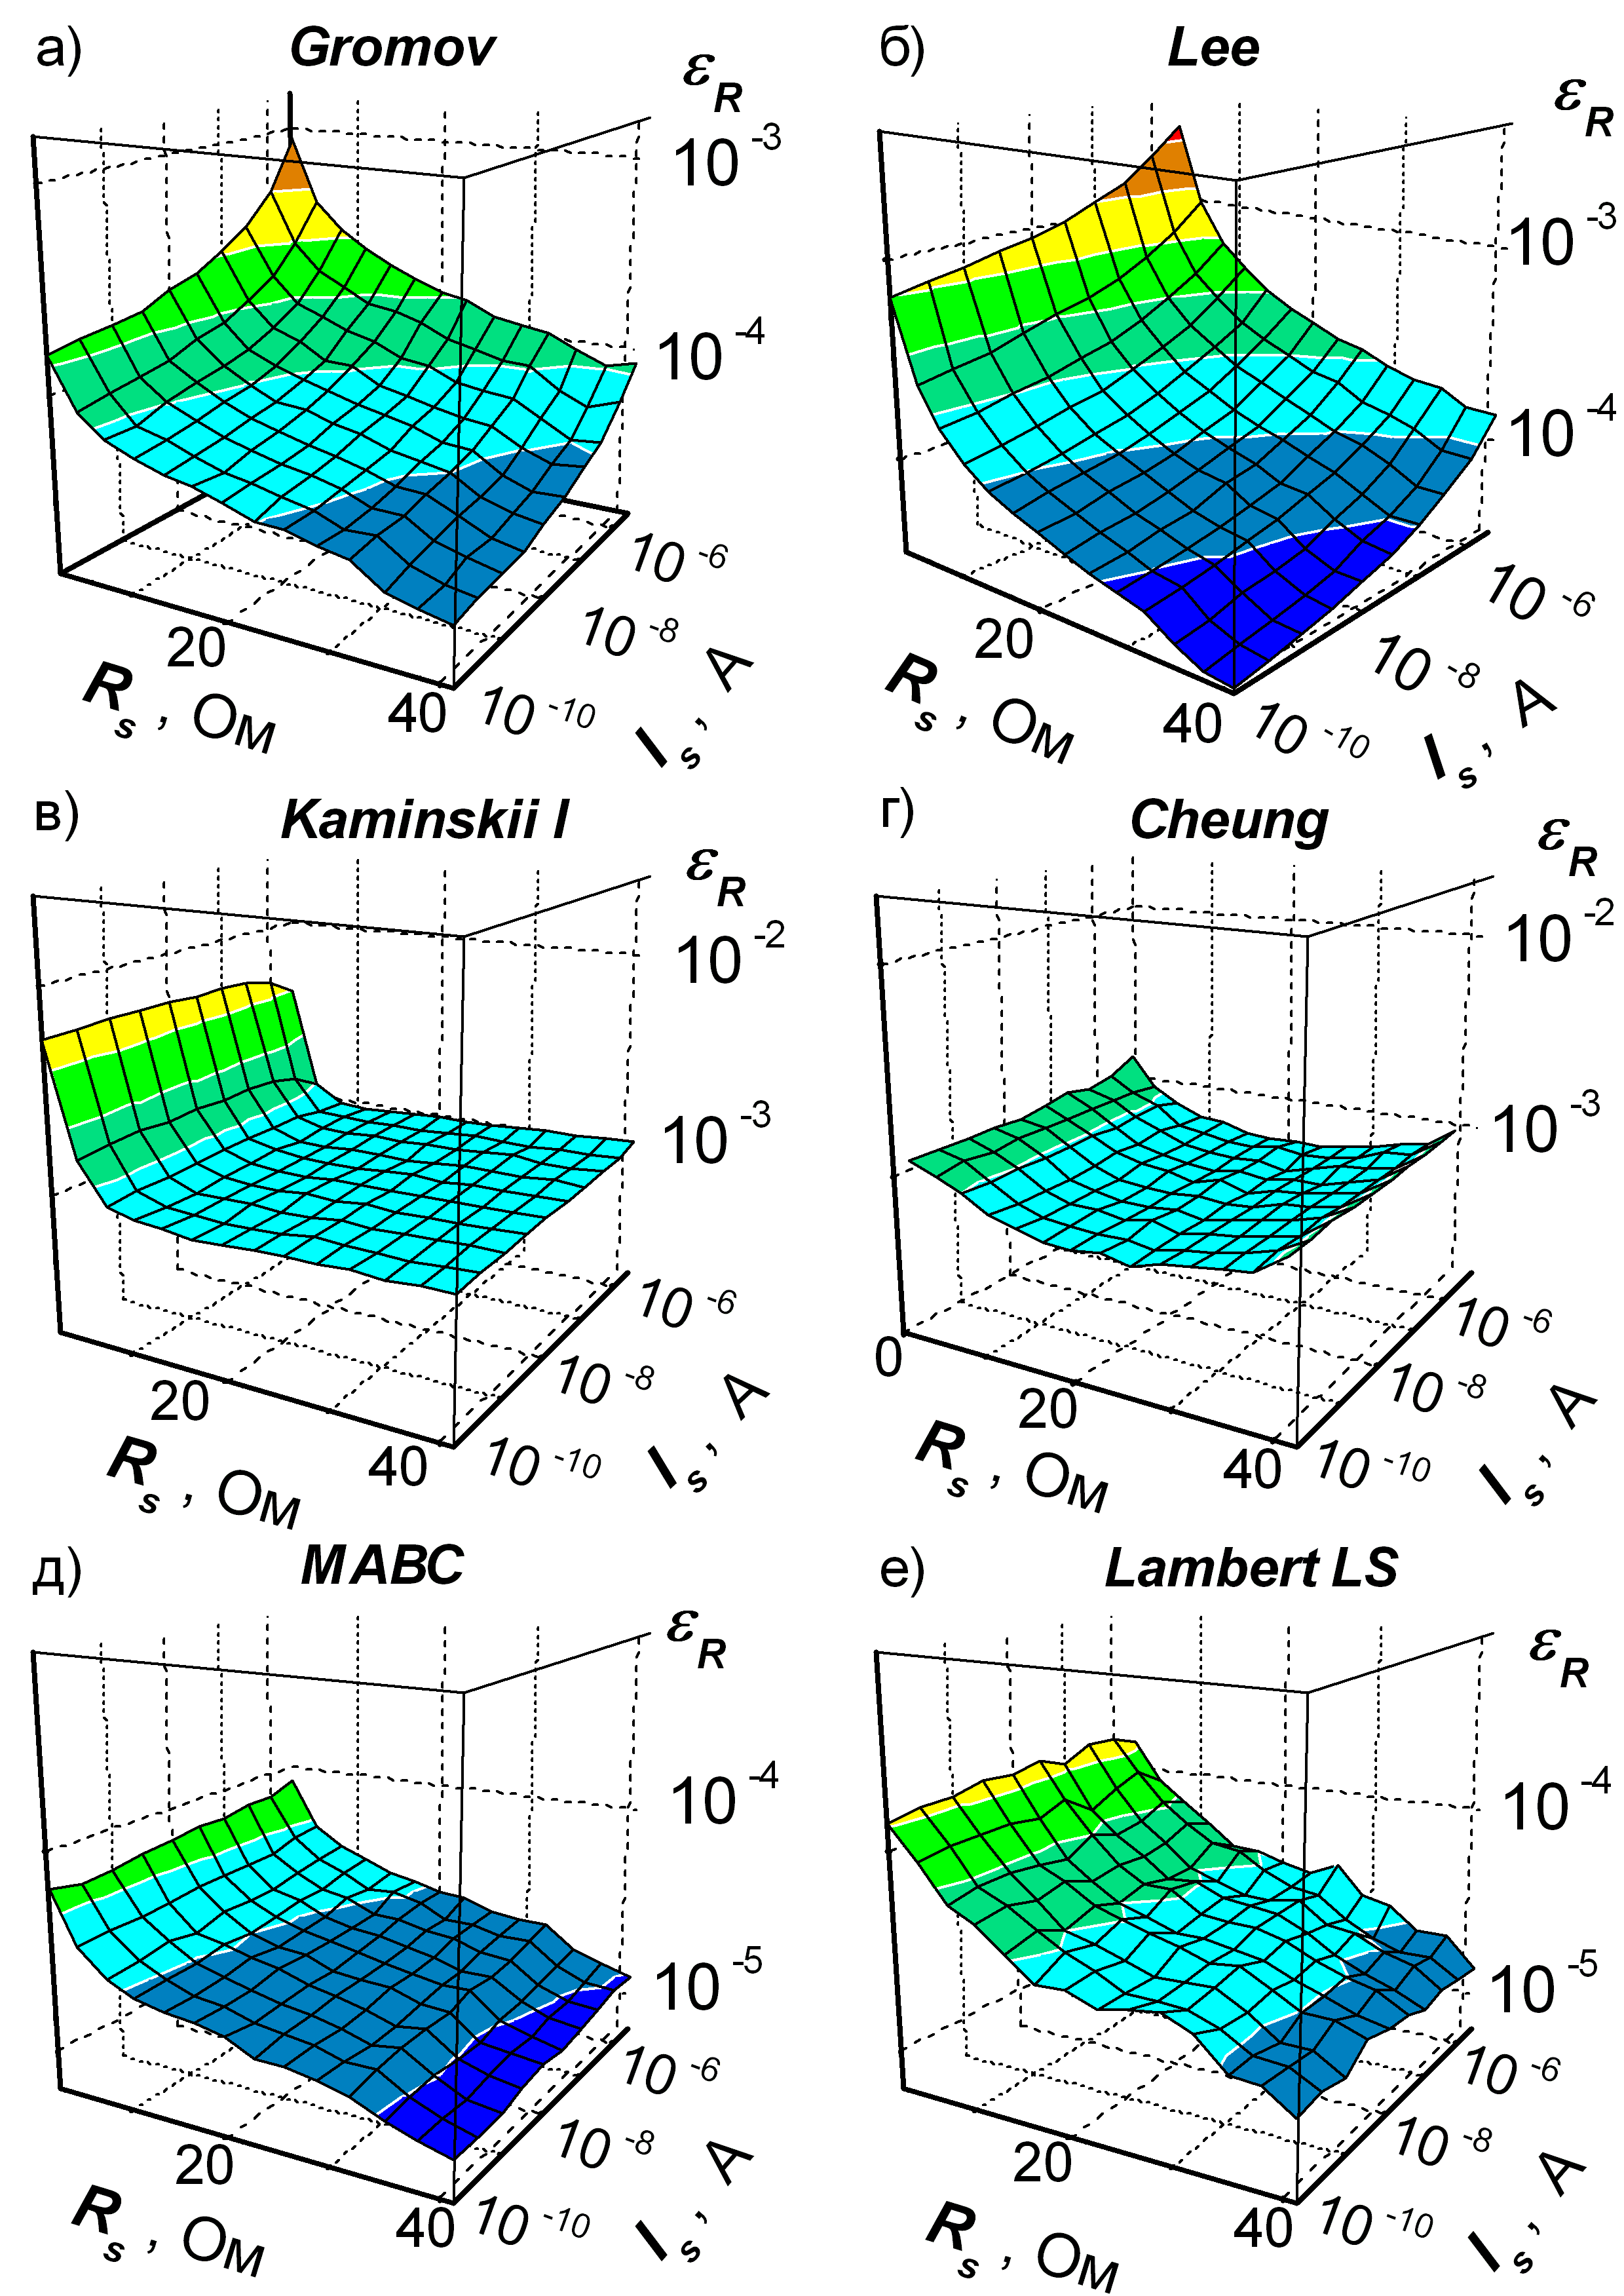
\includegraphics[width=0.8\textwidth]{figR3D}%
\caption{\label{figR3D}
Похибки визначення величини послідовного опору з набору ВАХ, який був синтезований при постійних значеннях $R_s$ та $I_s$.
Показані результати застосування методів Gromov (a), Lee (б), Kaminskii I (в), Cheung (г), MABC (д) та and Lambert LS (е).
}
\end{figure}

\begin{figure}
\center
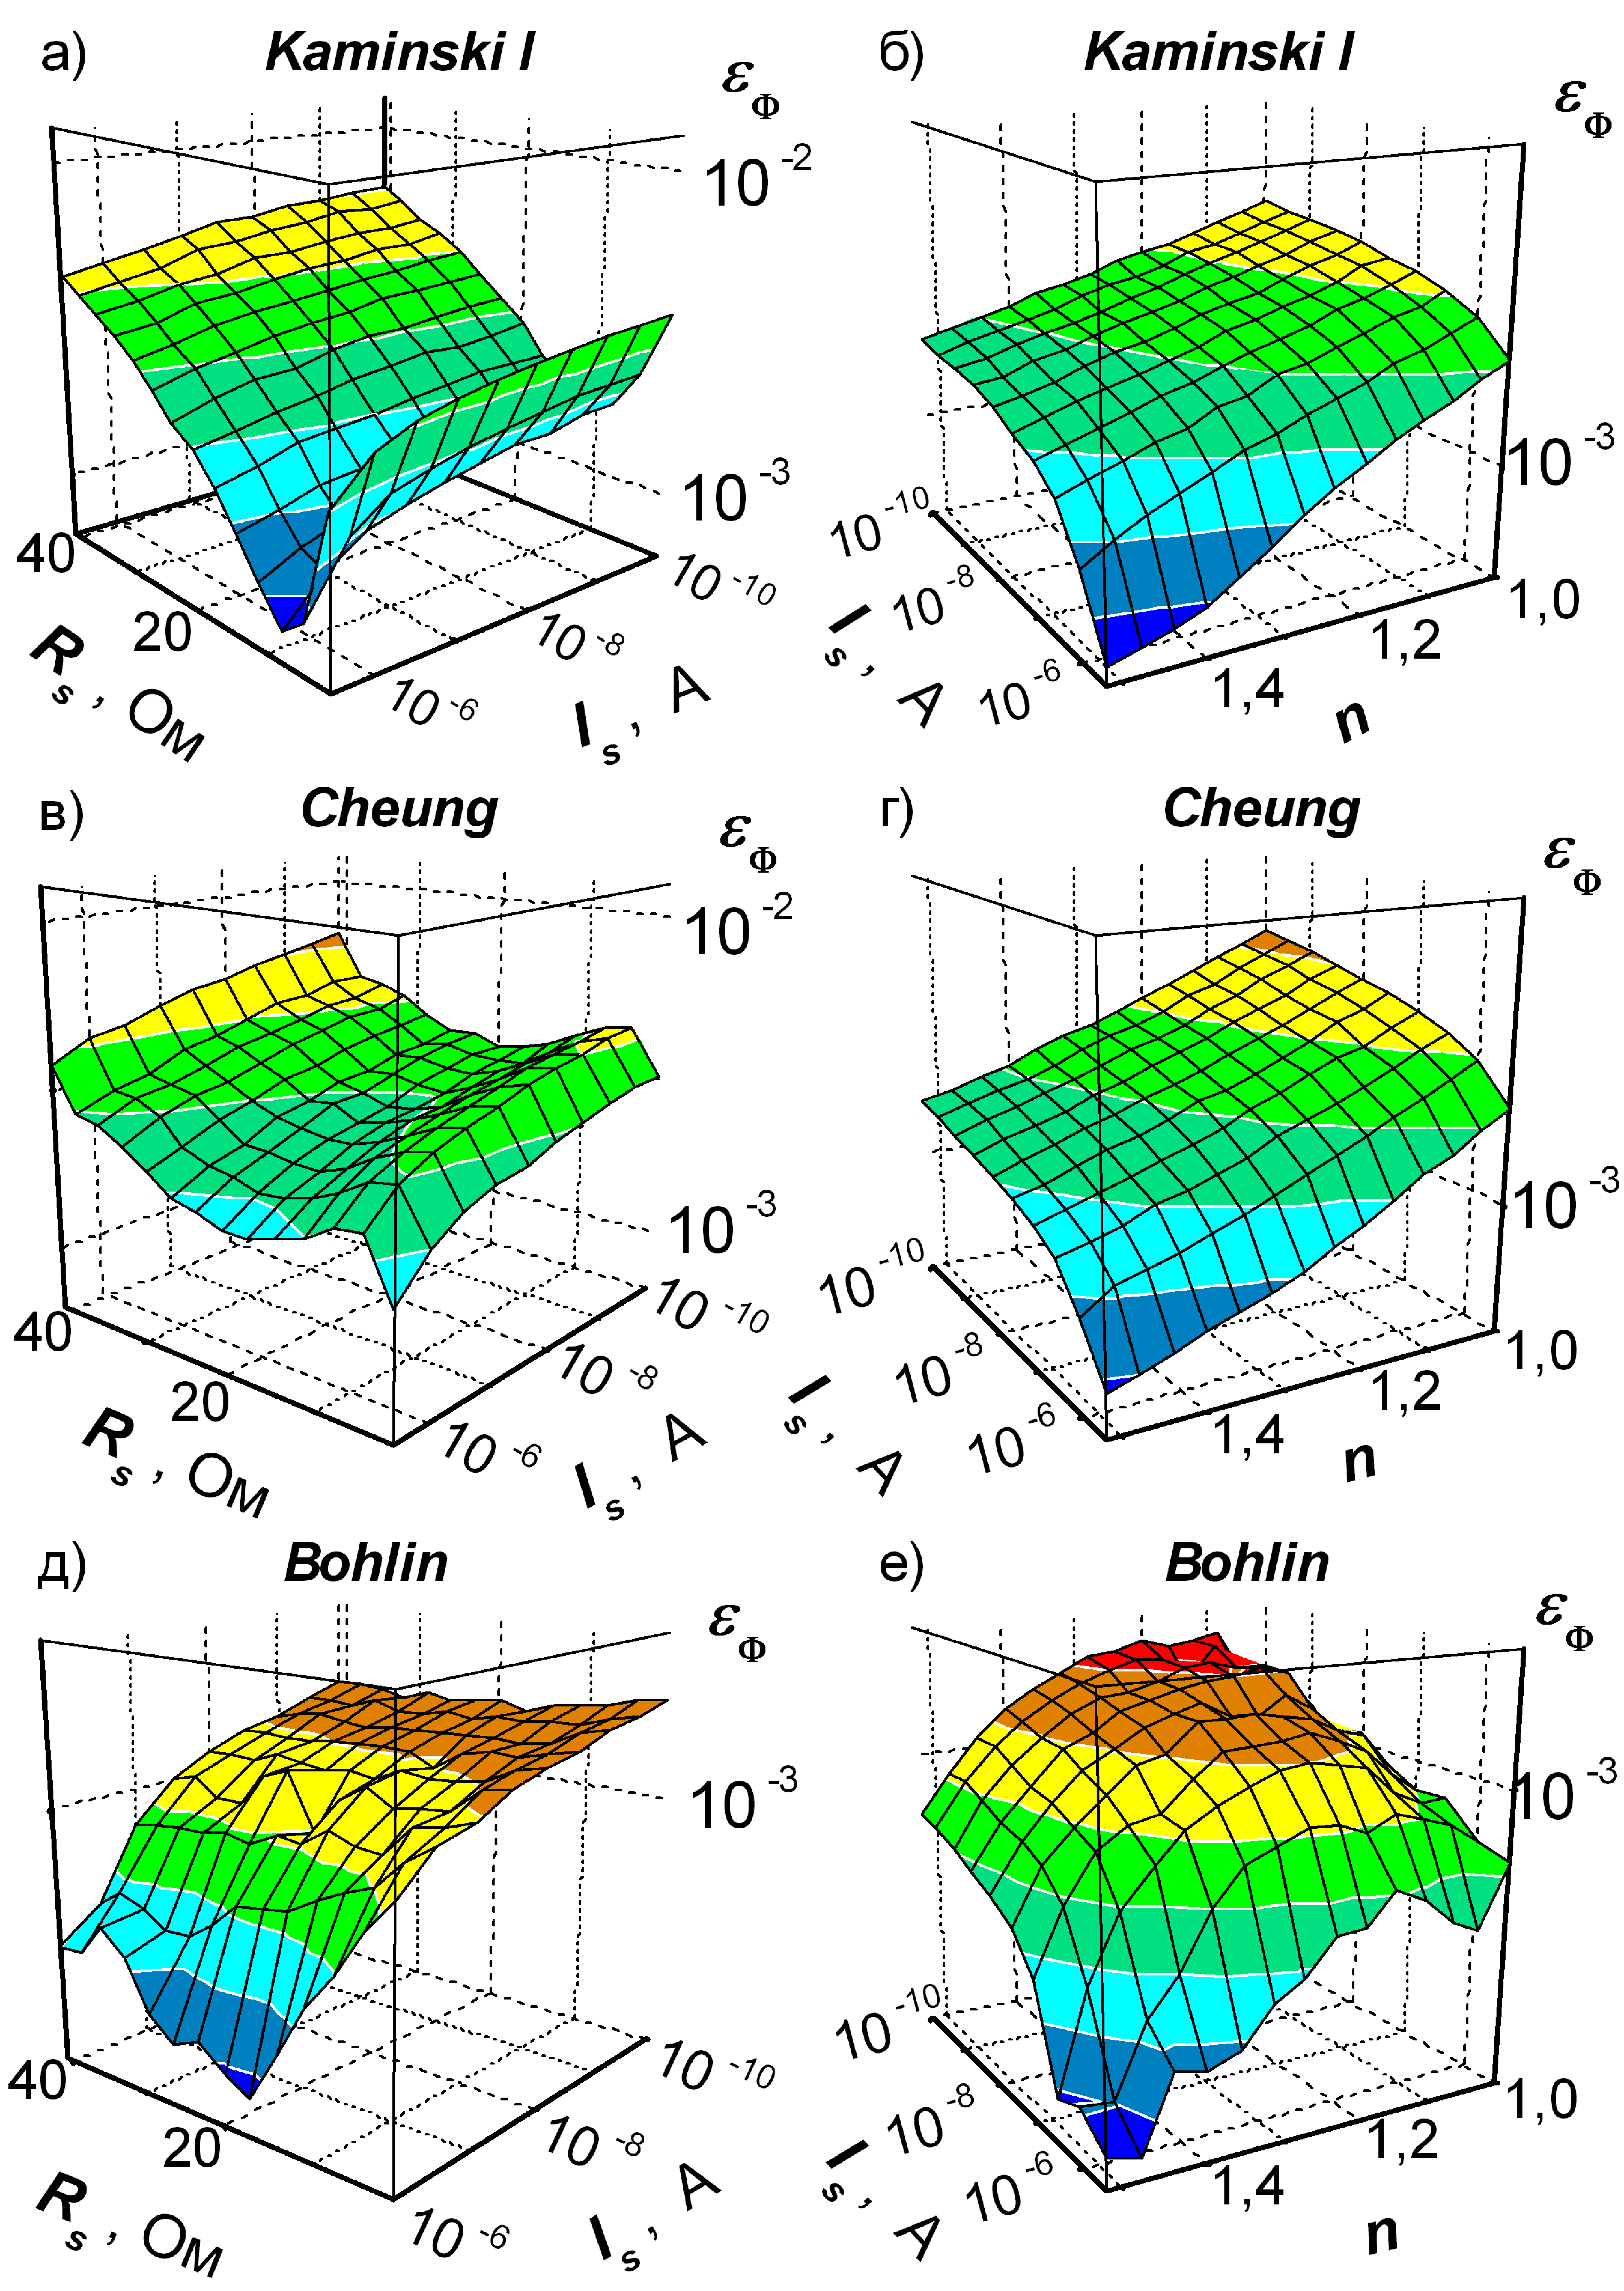
\includegraphics[width=0.8\textwidth]{figF3D}%
\caption{\label{figF3D}
Похибки визначення величини висоти бар'єру Шотки опору з набору ВАХ, який був синтезований при постійних значеннях $R_s$ та $I_s$ (рисунки а, в та д) або постійних значеннях $n_\mathrm{id}$ та $I_s$ (рисунки б, г, е).
Показані результати застосування методів Kaminskii I (a, б), Cheung (в, г) та Bohlin (д, е).
}
\end{figure}


\begin{figure}
\center
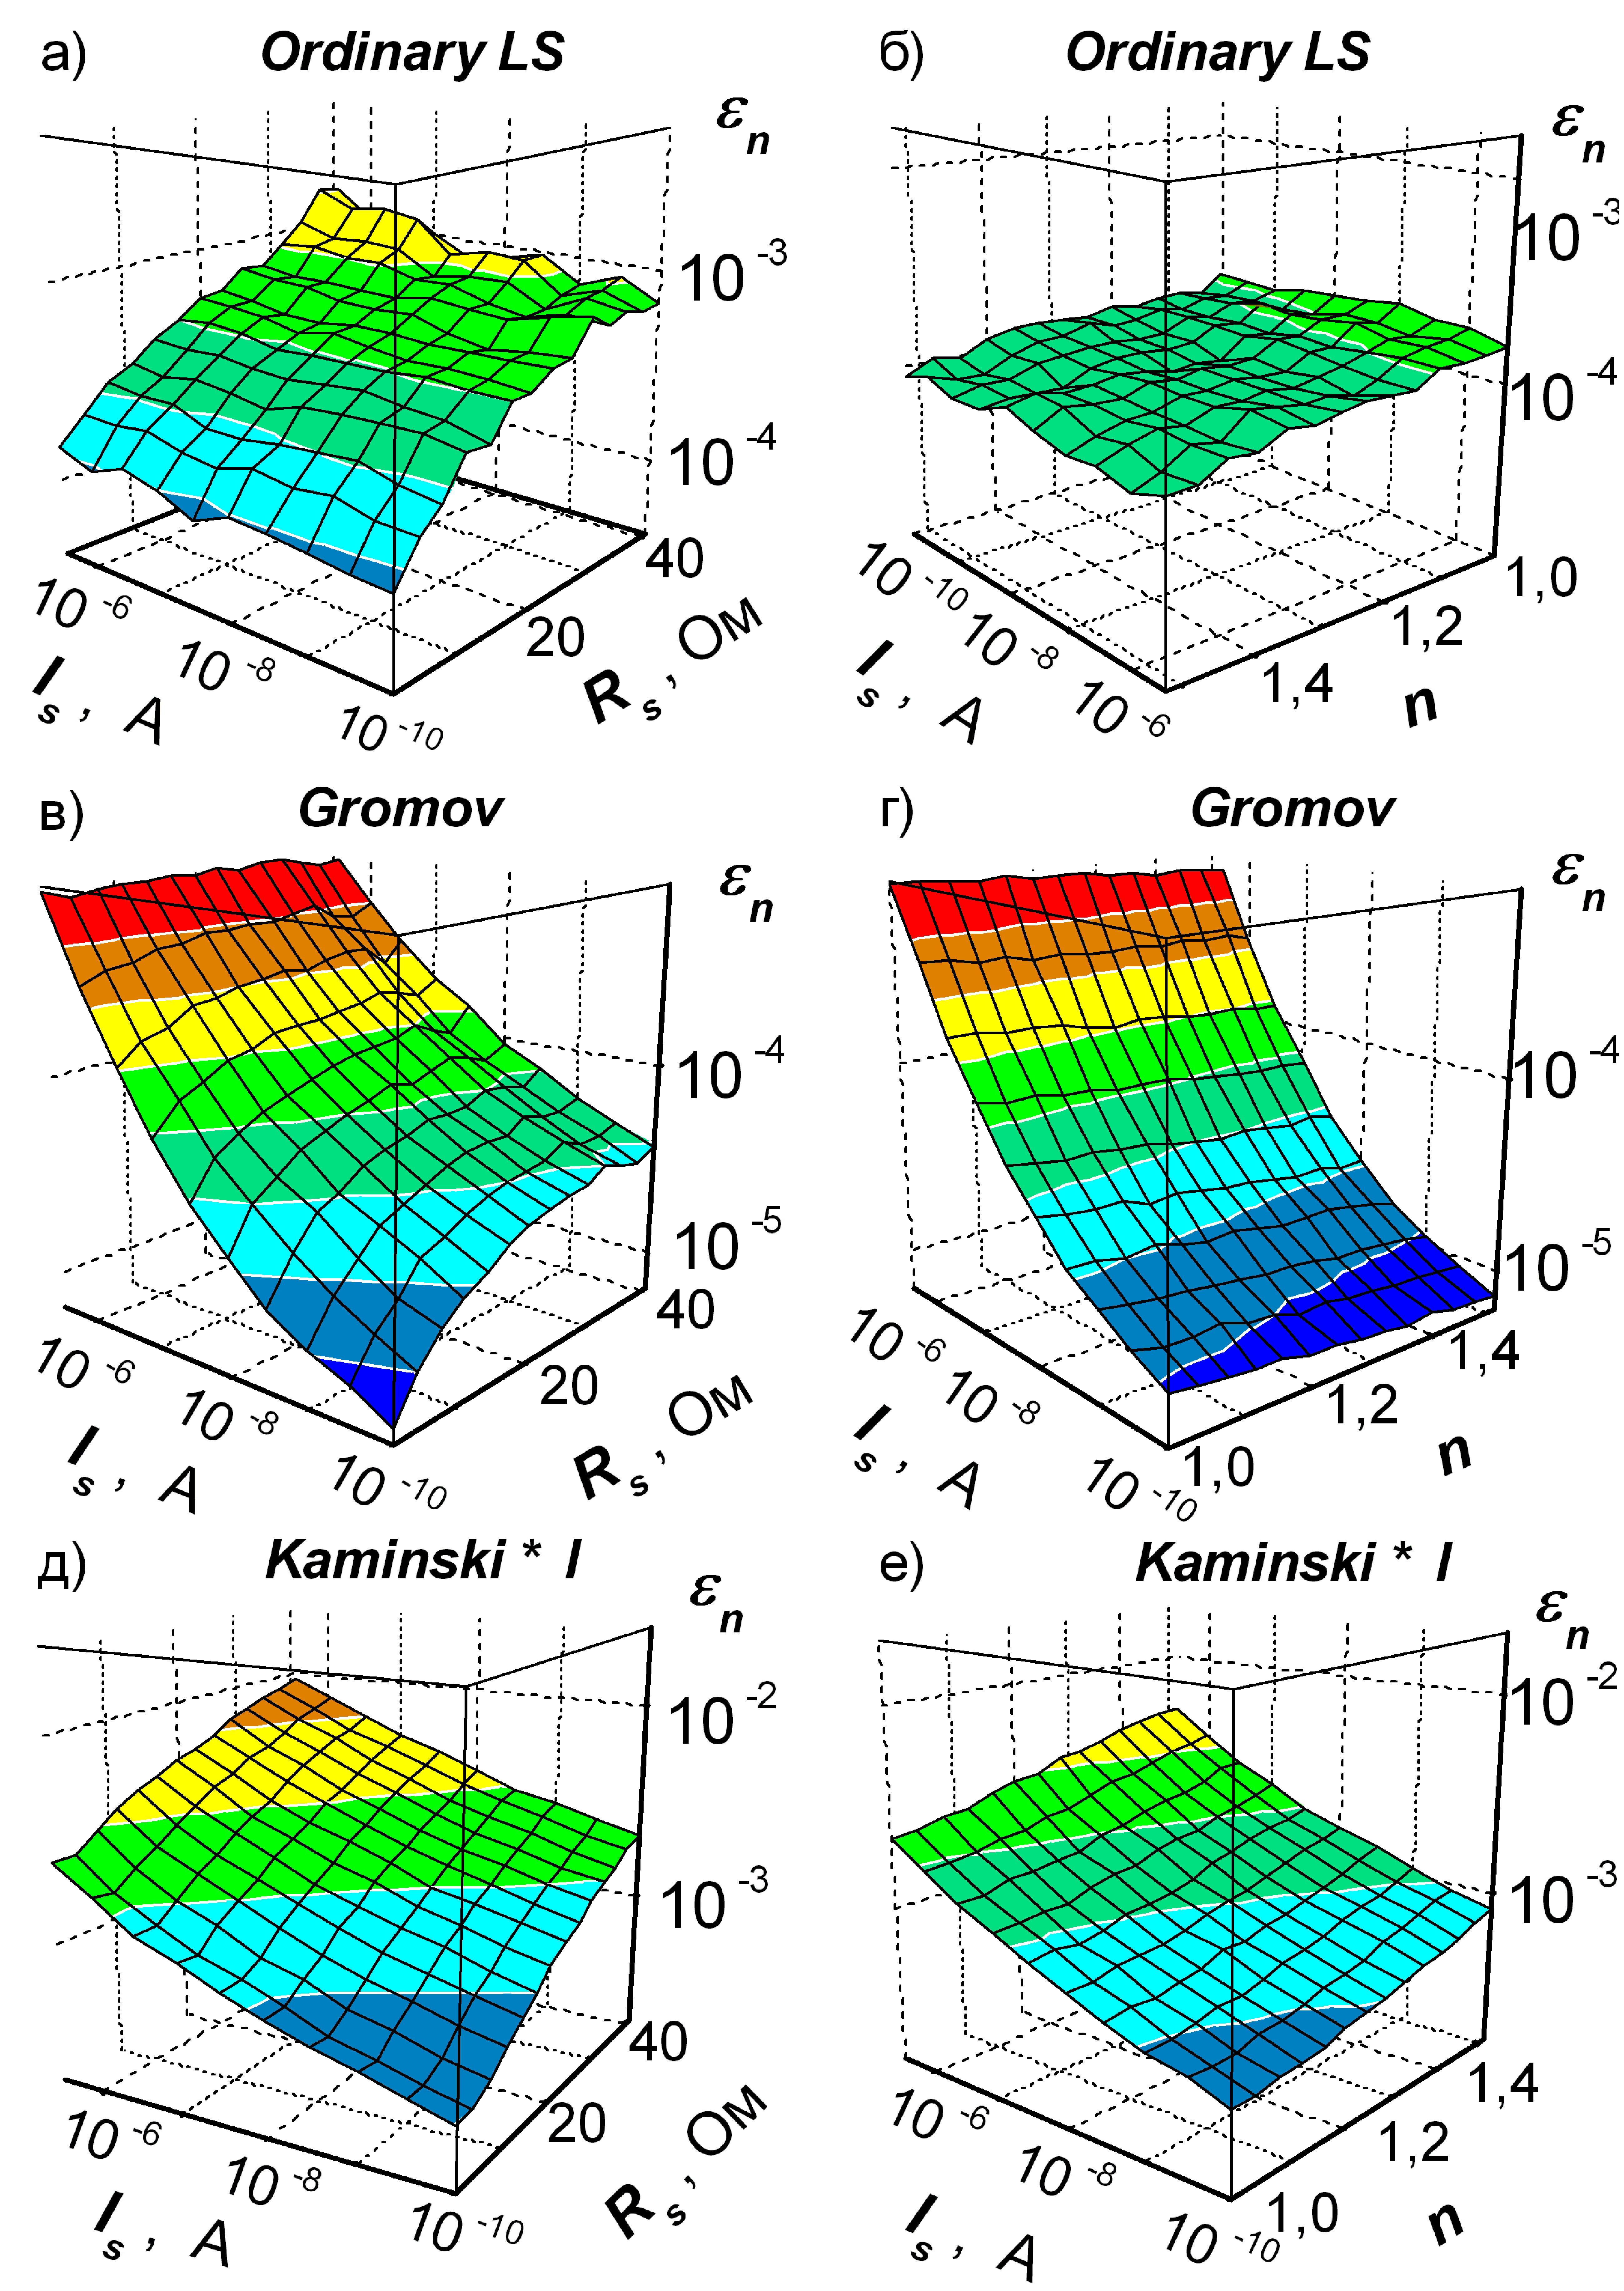
\includegraphics[width=0.8\textwidth]{fign3D}%
\caption{\label{fign3D}
Похибки визначення величини фактору неідеальності з набору ВАХ, який був синтезований при постійних значеннях $R_s$ та $I_s$ (рисунки а, в та д) або постійних значеннях $n_\mathrm{id}$ та $I_s$ (рисунки б, г, е).
Показані результати застосування методів Ordinary LS (a, б), Gromov (в, г) та Kaminskii*~I (д, е).
}
\end{figure}

Для того, щоб виявити основні тенденції цих залежностей були проведені додаткові дослідження.
А саме, були синтезовані набори ВАХ, при побудові яких вважалося, що деякі параметри є незалежними від температури.
В цьому випадку
а)~постійними у всьому температурному діапазоні вважалася два параметри ($R_s$ та $I_s$  або $n_\mathrm{id}$ та $I_s$ для різних наборів ВАХ);
б)~$n_\mathrm{id}$ (або $R_s$) розраховувалися відповідно до того, як описано раніше, в розділі~\ref{SubData}.
Було створено сукупність наборів ВАХ, для яких незалежні від температури величини $R_s$, $n_\mathrm{id}$ та $I_s$ змінювались в діапазонах від
2 до 41~Ом, від 1 до 1,52 та від $10^{-10}$ до $5\cdot10^{-5}$~A, відповідно.
Після цього кожен з методів було застосована до кожного з набору ВАХ, визначено величини параметрів, а також їх похибки.
Найбільш типові результати наведено ни Рис.~\ref{figR3D}--\ref{fign3D}.
Зокрема, Рис.~\ref{figR3D},a підтверджує, що при використанні методу Gromov збільшення $R_s$ та $I_s$ призводить до зменшення та збільшення помилки визначення послідовного опору, відповідно.


Отримані результати щодо факторів впливу узагальнено в Таблиці~\ref{tabIF}.
В цій таблиці використано ряд символів для опису поведінки похибки визначення параметрів при зміні величини фактору впливу.
А саме.
Якщо помилка визначення монотонно зростає або зменшується зі збільшенням впливаючого фактору, то використовувались символи <<$\downarrow$>> та <<$\uparrow$>>, відповідно.
Наприклад, саме ці символи характеризують кореляцію точності визначення $R_s$ за допомогою методу Gromov та величини $R_s$ та $I_s$.



\begin{table}
\caption{\label{tabIF}Фактори впливу на похибки визначення параметрів ДШ.$^{1)}$
%\footnote{The presence of $R_s$ or $I_s$ or $n$ in the cell indicates the impact on extracted parameter accuracy;
%the subscript and inside bracket symbol deal with extraction error behavior with influencing factor increasing --- see details in the text.}
}
\centering
\small
\begin{tabular}{|l|c|c|c|}
%\begin{tabularx}{\textwidth}{|l|
%                              >{\centering\arraybackslash}X|
 %                             >{\centering\arraybackslash}X|
  %                            >{\centering\arraybackslash}X|}
\hline
\multicolumn{1}{|c|}{Метод}&\multicolumn{3}{c|}{Визначений параметр}\\
\cline{2-4}
%\hline
 &$R_s$&$\Phi_b$&$n$\\
%Метод &$R_s$&$\Phi_b$&$n$\\
%\hline
%\hline
\hhline{|====|}
Norde &$n_\mathrm{id}^w(\vee)$&$I_s(\downarrow)$&---\\
\hline
Werner &$R_s(\vee)$&$R_s(\downarrow)$, $I_s^w(\downarrow)$, $n_\mathrm{id}^w(\downarrow)$&$R_s(\uparrow)$, $n_\mathrm{id}^w(\downarrow)$\\
\hline
Werner* &$R_s(\vee)$&$R_s(\vee)$, $I_s(\uparrow)$, $n_\mathrm{id}(\uparrow)$&$R_s(\vee)$, $I_s(\uparrow)$, $n_\mathrm{id}^w(\uparrow)$\\
\hline
Cibils &$R_s(\vee)$, $n_\mathrm{id}(\uparrow)$&$R_s(\uparrow)$, $n_\mathrm{id}(\vee)$& $R_s(\uparrow)$, $n_\mathrm{id}(\vee)$\\
\hline
Cibils* &$R_s(\vee)$, $n_\mathrm{id}(\uparrow)$&$R_s(\vee)$, $I_s(\uparrow)$, $n_\mathrm{id}(\uparrow)$& $R_s(\vee)$, $I_s(\uparrow)$, $n_\mathrm{id}(\uparrow)$\\
\hline
Kaminskii I&$R_s(\leftharpoonup)$, $n_\mathrm{id}^w(\downarrow)$&$R_s(\vee)$, $I_s(\downarrow)$, $n_\mathrm{id}(\downarrow)$& $R_s(\vee)$, $I_s^w(\downarrow)$, $n_\mathrm{id}(\downarrow)$\\
\hline
Kaminskii* I&$R_s(\leftharpoonup)$, $n_\mathrm{id}^w(\downarrow)$&$R_s(\uparrow)$, $I_s(\uparrow)$, $n_\mathrm{id}(\uparrow)$& $R_s(\uparrow)$, $I_s(\uparrow)$, $n_\mathrm{id}(\uparrow)$\\
\hline
Kaminskii II&$R_s(\downarrow)$, $I_s(\rightharpoonup)$, $n_\mathrm{id}^w(\uparrow)$&$I_s(\rightharpoonup)$, $n_\mathrm{id}^w(\uparrow)$& $I_s(\rightharpoonup)$\\
\hline
Kaminskii* II&$R_s(\downarrow)$, $I_s(\rightharpoonup)$, $n_\mathrm{id}^w(\uparrow)$&$I_s(\uparrow)$, $n_\mathrm{id}(\uparrow)$& $I_s(\uparrow)$, $n_\mathrm{id}(\uparrow)$\\
\hline
Bohlin &$I_s(\rightharpoondown)$&$I_s(\downarrow)$, $n_\mathrm{id}(\wedge)$& $I_s(\rightharpoondown)$, $n_\mathrm{id}(\wedge)$\\
\hline
Lee &$R_s(\downarrow)$, $I_s(\uparrow)$, $n_\mathrm{id}(\uparrow)$&$I_s(\uparrow)$, $n_\mathrm{id}(\uparrow)$& $I_s(\uparrow)$, $n_\mathrm{id}(\uparrow)$\\
\hline
Gromov &$R_s(\downarrow)$, $I_s(\uparrow)$&$R_s(\uparrow)$, $I_s(\uparrow)$, $n_\mathrm{id}^w(\downarrow)$&$R_s(\uparrow)$, $I_s(\uparrow)$, $n_\mathrm{id}^w(\downarrow)$\\
\hline
Cheung &$R_s^w(\vee)$&$R_s(N)$, $I_s(\downarrow)$, $n_\mathrm{id}(\downarrow)$&$R_s^w(N)$, $I_s(\rightharpoondown)$, $n_\mathrm{id}(\downarrow)$\\
\hline
Mikhelashvili &$R_s(\uparrow)$, $I_s(\downarrow)$, $n_\mathrm{id}^w(\downarrow)$&$R_s(\uparrow)$, $I_s(\wedge)$, $n_\mathrm{id}^w(\downarrow)$&$R_s(\uparrow)$, $I_s(\wedge)$, $n_\mathrm{id}^w(\downarrow)$\\
\hline
Ordinary LS &$R_s(\downarrow)$&$R_s(\uparrow)$, $I_s^w(\downarrow)$, $n_\mathrm{id}^w(\downarrow)$&$R_s(\uparrow)$, $n_\mathrm{id}^w(\downarrow)$\\
\hline
Lambert LS &$R_s(\downarrow)$&$I_s^w(\downarrow)$&$n_\mathrm{id}^w(\downarrow)$\\
\hline
EAs &$R_s(\downarrow)$, $I_s^w(\uparrow)$&$R_s(\uparrow)$, $I_s(\vee)$, $n_\mathrm{id}^w(\downarrow)$&$R_s(\uparrow)$, $I_s(\vee)$, $n_\mathrm{id}^w(\downarrow)$\\
\hline
\multicolumn{4}{|p{0.9\textwidth}|}{$^{1}$\textit{Наявність $R_s$ або $I_s$ або $n_\mathrm{id}$ в клітинці означає
вплив величини, відповідно, послідовного опору або струму насичення або фактору неідеальності на точність визначення параметру;
верхній індекс та символ в дужках пов'язані з характером поведінки точності визначення параметру при збільшенні $R_s$ або $I_s$ або $n_\mathrm{id}$ --- деталі див. у тексті.
}}\\
\hline
\end{tabular}
%\end{tabularx}
\end{table}

Виявлено, може залежати від фактору впливу не лише монотонно.
Наприклад, Рис.~\ref{figCon},б та Рис.~\ref{figF3D},a показують, що при використанні методу Kaminskii~I похибка визначення $\Phi_b$ зростає з підвищенням послідовного опору при великих ($>10$~Ом) значеннях $R_s$ і зменшується при малих величинах $R_s$.
Для позначення залежності з такою поведінкою в Таблиці~\ref{tabIF} використовується символ <<$\vee$>>.
Подібна залежність спостерігається при використанні метода Chueng для визначення $R_s$ --- див. Рис.~\ref{figR3D},г.
Проте в цьому випадку сама величина $R_s$ порівняно слабко впливає на точність визначення послідовного опору.
Схожі слабкі залежності позначаються в Таблиці~\ref{tabIF} за допомогою верхнього індексу  <<$w$>>.
Інші приклади слабких залежностей $I_s$ та  $n_\mathrm{id}$ можна побачити на Рис.~\ref{figR3D},д та Рис.~\ref{fign3D},г, відповідно.

Якщо графік залежності похибки визначення параметру від величини фактору впливу має не мінімум, а максимум (див., наприклад, Рис.~\ref{figF3D},е),
то використовувався символ <<$\wedge$>>.
Наявність на залежності екстремумів обох типів (див., наприклад, Рис.~\ref{figF3D},в) позначено за допомогою символу <<$N$>>.

Ще один тип залежності показаний на Рис.~\ref{figR3D},в.
При використанні методу Kaminskii~I для визначення  $R_s$ помилки залишаються постійними в широкому діапазоні змін $R_s$ та $I_s$ і зростають лише для малих значень $R_s$.
Подібні залежності між помилкою визначення та впливаючим фактором позначені символом <<$\leftharpoonup$>>.
Символи <<$\rightharpoonup$>> або <<$\rightharpoondown$>> якщо помилки зростають або зменшуються, відповідно, лише при великих значеннях фактору впливу.

З наведених даних, зокрема, видно, що фактори, які впливають на точність екстракції $\Phi_b$ та  $n_\mathrm{id}$ подібні для більшості методів, які розглядалися в роботі.
Використання адаптивної процедури в методі Gromov призводить до того, що точність визначення $\Phi_b$ та  $n_\mathrm{id}$ стає залежною від величини $R_s$, тоді як вплив величини фактору неідеальності послаблюється.
Точність методів Werner*, Cibils* та Kaminskii* більш чутлива до величин параметрів ніж при використанні варіантів цих же методів без зірочок.
Найбільш стійкими до величин параметрів є точності чисельних методів, особливо при використанні функції Ламберта (Lambert LS).


\subsection{Швидкодія методів визначення параметрів діодів Шотки}
Ще одним, поряд з точністю, критерієм для характеризації різних методів визначення параметрів структур МН є час, необхідний для визначення параметрів (RT, running time).
Для оцінки RT були використані WinAPI функції $QueryPerformanceCounter()$ та $QueryPerformanceFrequency()$.
Розрахунки проводились на персональному комп'ютері з наступними характеристиками:
\begin{itemize}
  \item процесор AMD A4-3400 2.7~GHz;
  \item 3072~MB RAM;
  \item операційна система Windows XP.
\end{itemize}
Очевидно, що точний час екстракції параметрів залежить від програмної реалізації, від завантаження процесору в даний момент часу тощо.
Тим не менш, всі методи тестувалися за однакових умов, а отже вибраний підхід дозволяє порівняти тривалість роботи різних методів, а також оцінити порядок величини RT.

\begin{table}
\caption{\label{tabRT}Час визначення параметрів ДШ з однієї ВАХ.}
\begin{tabularx}{\textwidth}{|>{\raggedright\arraybackslash}X|
                             >{\centering\arraybackslash}X|
                            >{\centering\arraybackslash}X|}
\hline
\multicolumn{1}{|c|}{Метод}&\multicolumn{2}{c|}{Час роботи, с}\\
\cline{2-3}
%\begin{tabular}{lcc}
%Method &\multicolumn{2}{c}{Running time, s}\\
 &максимальний&мінімальний\\
\hhline{|===|}
Norde &$3,7\cdot10^{-5}$&$2,6\cdot10^{-5}$\\ \hline
Werner $^{1)}$ &$4,5\cdot10^{-5}$&$4,0\cdot10^{-5}$\\ \hline
Cibils $^{1)}$ &$5,3\cdot10^{-3}$&$1,9\cdot10^{-4}$\\ \hline
Kaminskii I $^{1)}$ &$8,0\cdot10^{-5}$&$4,5\cdot10^{-5}$\\ \hline
Kaminskii II $^{1)}$ &$2,6\cdot10^{-3}$&$3,0\cdot10^{-4}$\\ \hline
Bohlin &$6,3\cdot10^{-5}$&$4,0\cdot10^{-5}$\\ \hline
Lee &$3,6\cdot10^{-3}$&$1,8\cdot10^{-4}$\\ \hline
Gromov &$2,2\cdot10^{-2}$&$2,2\cdot10^{-2}$\\ \hline
Gromov $^{2)}$ &$4,6\cdot10^{-5}$&$2,7\cdot10^{-5}$\\ \hline
Cheung &$3,2\cdot10^{-5}$&$2,0\cdot10^{-5}$\\ \hline
Mikhelashvili &$4,7\cdot10^{-5}$&$2,9\cdot10^{-5}$\\ \hline
Ordinary LS &$460$&$1,8$\\ \hline
Lambert LS &$540$&$7,6$\\ \hline
DE &$0,73$&$0,36$\\ \hline
PSO &$0,35$&$0,14$\\ \hline
MABC &$0,20$&$5,7\cdot10^{-2}$\\ \hline
TLBO &$19,2$&$5,4$ \\
\hline
\multicolumn{3}{|p{17cm}|}{$^{1}$\textit{Час корекції ВАХ та лінійної апроксимації дорівнює $1.8\cdot10^{-5}$~с (максимальний) або $1.4\cdot10^{-5}$~с (мінімальний)}.
}\\
\multicolumn{3}{|p{17cm}|}{$^{2}$\textit{Для випадку, коли адаптивна процедура не використовується}.
}\\ \hline
\end{tabularx}
\end{table}

Отримані значення RT при застосуванні різноманітних методів до аналізу ідеальних синтезованих ВАХ наведено в Таблиці~\ref{tabRT}.
Загалом, RT залежить від кількості точок у вихідній залежності;
в таблиці наведено значення, отримані при застосування методів до ВАХ, сгенерованих для температур 130~K та 330~K.
Очевидно, що
\begin{enumerate}[label=\asbuk*),leftmargin=0em,itemindent=1.5em]
\item час роботи аналітичних методів при використанні сучасних комп'ютерів знехтувано малий;
\item у випадку ВАХ з великою кількістю експериментальних точок RT чисельних методів може досягати значних величин;
\item використання функції Ламберта призводить до збільшення часу роботи чисельних методів; однією з причин цього є необхідність використовувати числовий ряд для обчислення значення самої функції;
\item використання адаптивної функції очікувано викликає збільшення RT на декілька порядків, проте його абсолютне значення залишається невеликим;
\item серед еволюційних алгоритмів найбільш швидким при визначенні параметрів ДШ є MABC, тоді як найбільш повільним --- TLBO.
\end{enumerate}


Узагальнюючи результати, отримані при дослідженні застосування методів до ідеальних синтезованих ВАХ, зауважимо,
що еволюційні алгоритми видаються найбільш придатними для визначення параметрів ДШ завдяки низькому рівню помилок, помірній чутливості точності до величини параметрів
та допустимому часу роботи.
Поряд з цим, іншими методами, яким також варто надавати перевагу є аналітичний метод Gromov з використанням адаптивної процедури та числовий метод Lambert LS.
Проте, точність визначення параметрів для першого з них суттєво зменшується при високих значеннях струму насичення (високих температурах).
Щодо методу Lambert LS, то його основним недоліком є значний час, потрібний для обчислень.


\subsection{Вплив випадкових похибок на точність визначення параметрів структур метал--напівпровідник}

На Рис.~\ref{figG1003} та Рис.~\ref{figDiag} наведено результати застосування різноманітних методів до зашумлених даних.
Цілком очікувано, помилки при екстракції параметрів збільшуються при підвищенні рівня шуму (рівня випадкових помилок вимірювань).
Проте залежності правильності визначення параметрів з однієї ВАХ схожі до отриманих при аналізі ідеальних синтезованих ВАХ.
Як наслідок, фактори впливу на точність також ідентичні, тобто дані Таблиці~\ref{tabIF} цілком застосовні і в цьому випадку.
Крім того, інші характерні особливості методів, виявлені раніше, проявляються і в цьому випадку.
Наприклад, використання функції Ламберта дозволяє досягнути більшої точності чисельних методів при визначенні параметрів ДШ.
Еволюційні алгоритми, методи Gromov та Lee характеризуються найменшими помилками.
З іншого боку, різниця між результатами, отриманими за допомогою методів Gromov та Lee зменшується.
Це свідчить про зниження переваги застосування запропонованої адаптивної процедури з підвищенням рівня випадкових похибок.



\begin{figure}
\center
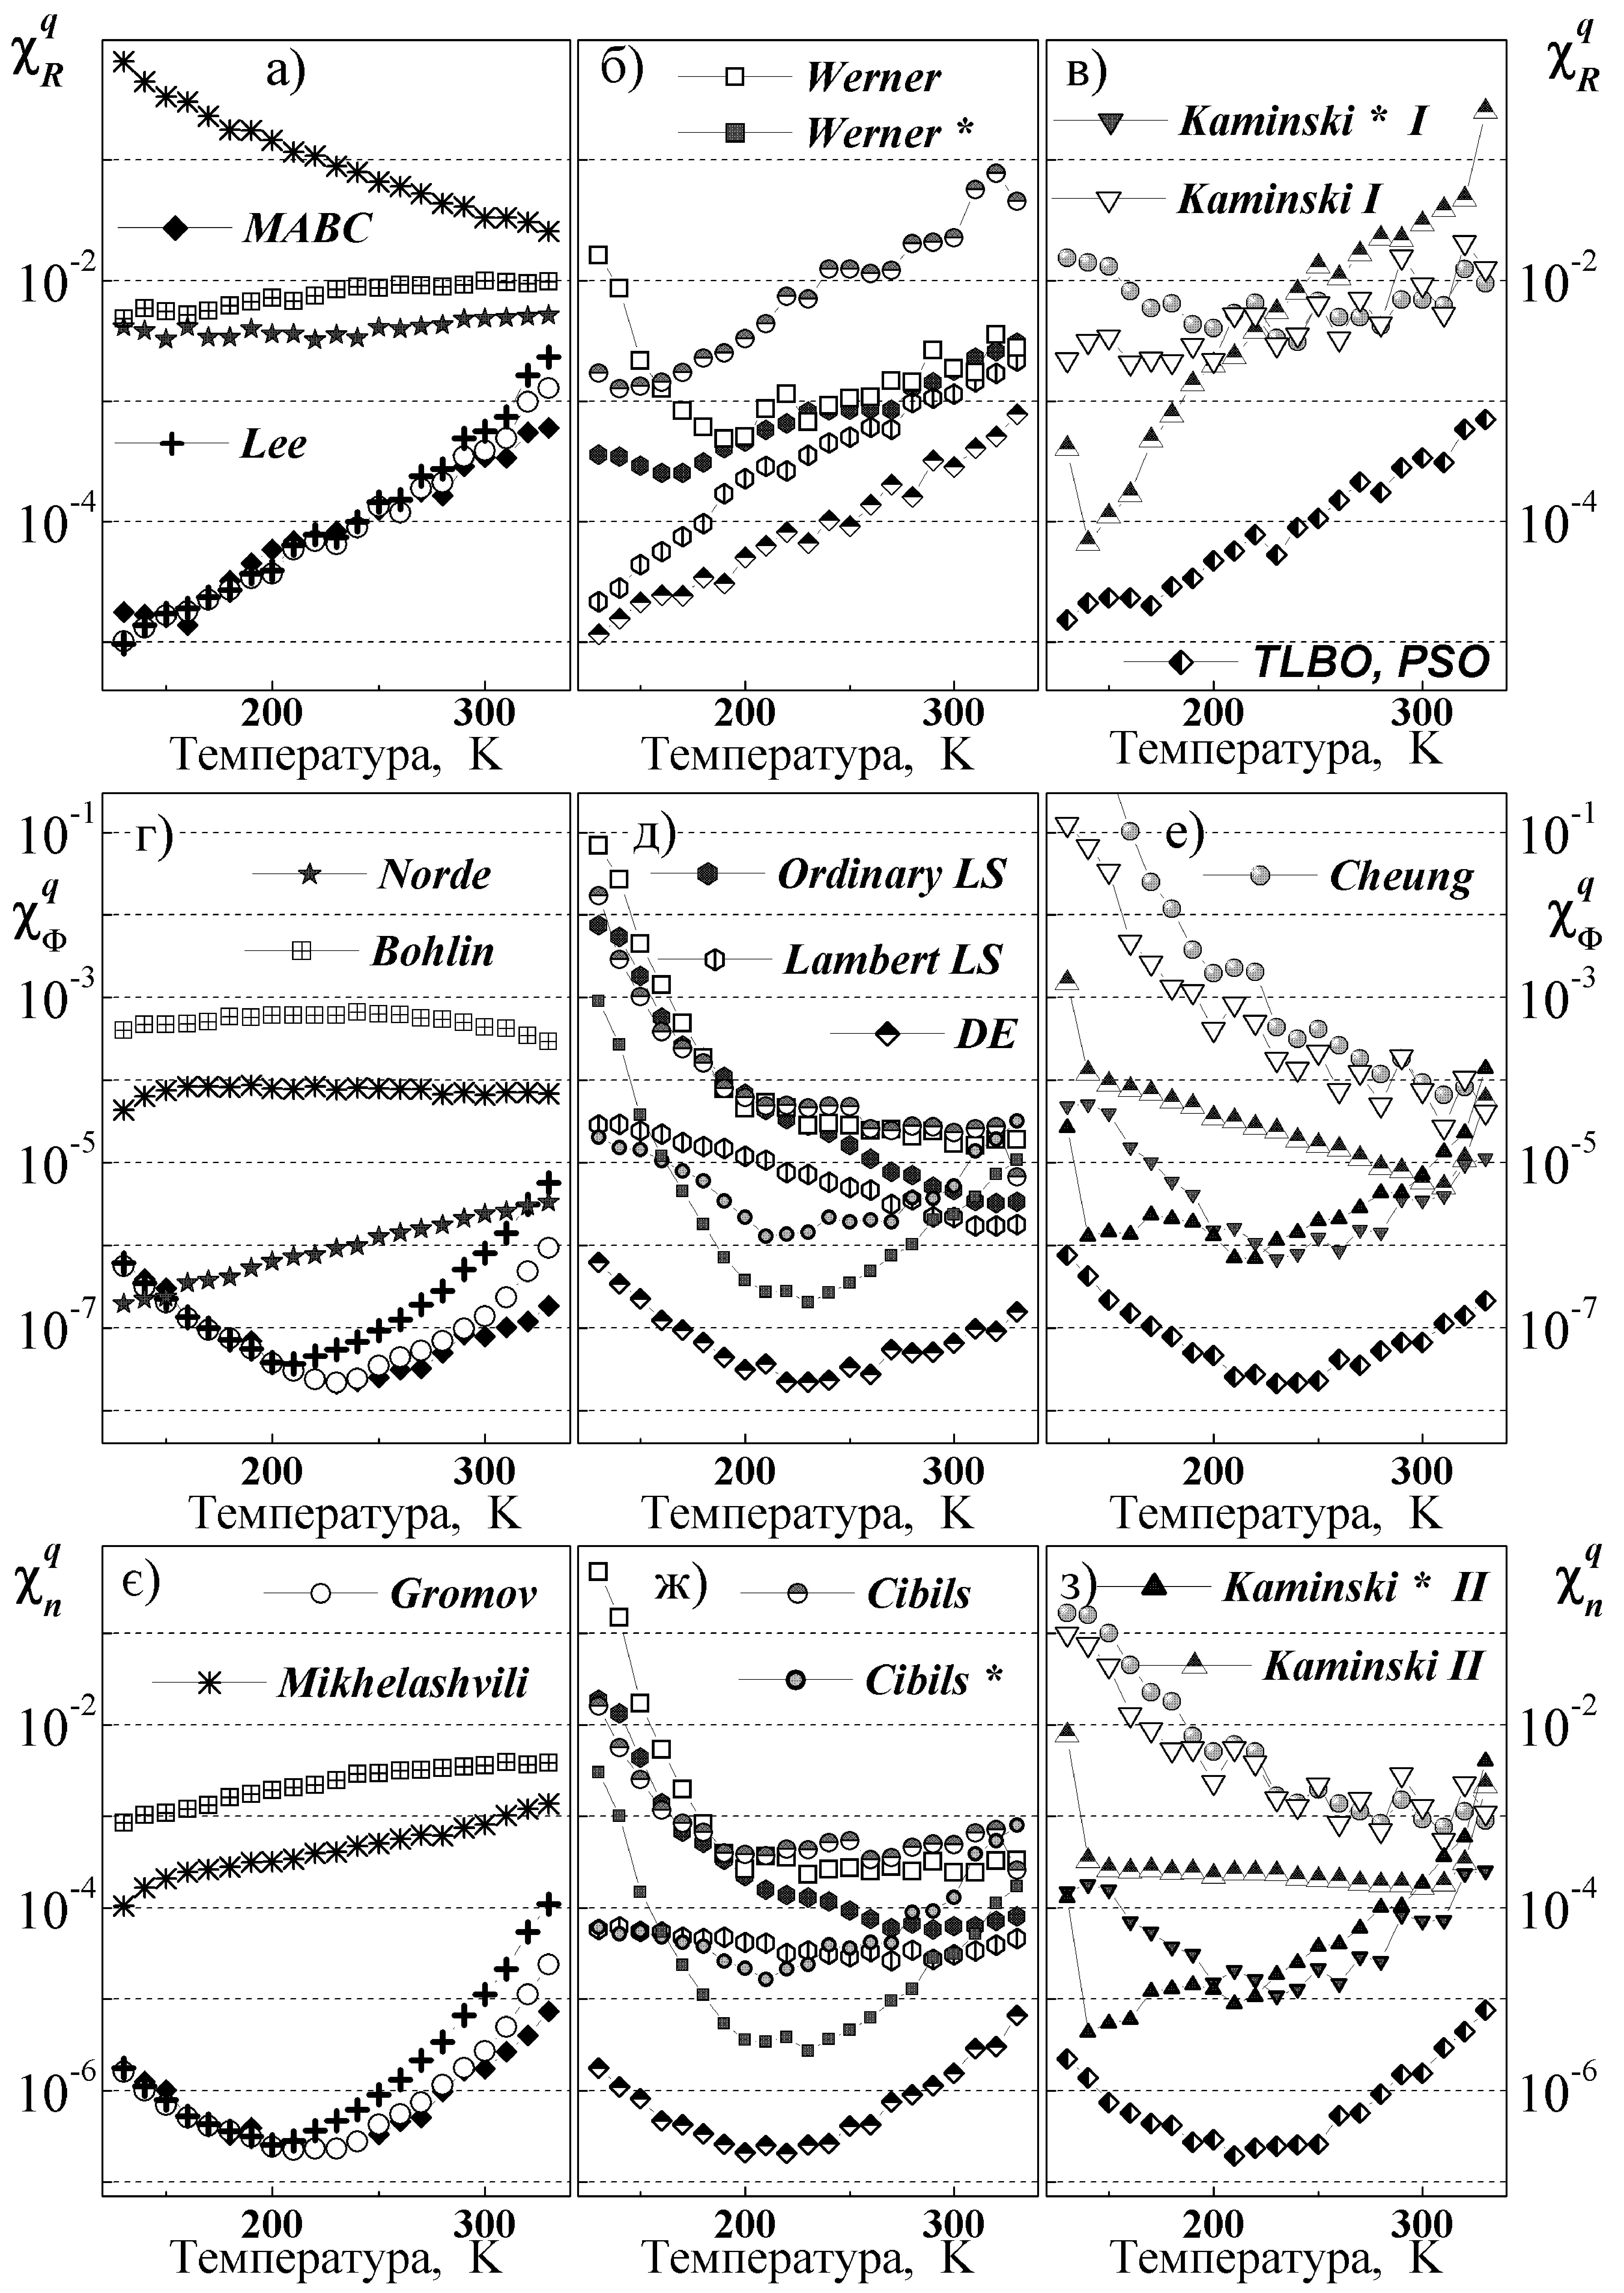
\includegraphics[width=0.8\textwidth]{figG1003}%
\caption{\label{figG1003}
Температурні залежності похибок визначення послідовного опору (а --- в), ВБШ (г --- е) та фактору неідеальності (є --- з) при застосуванні різних методів до наборів зашумлених даних.
$\sigma_V=0,3$~мВ, $\sigma_I^\varepsilon=1\%$.
}
\end{figure}

\begin{figure}
\center
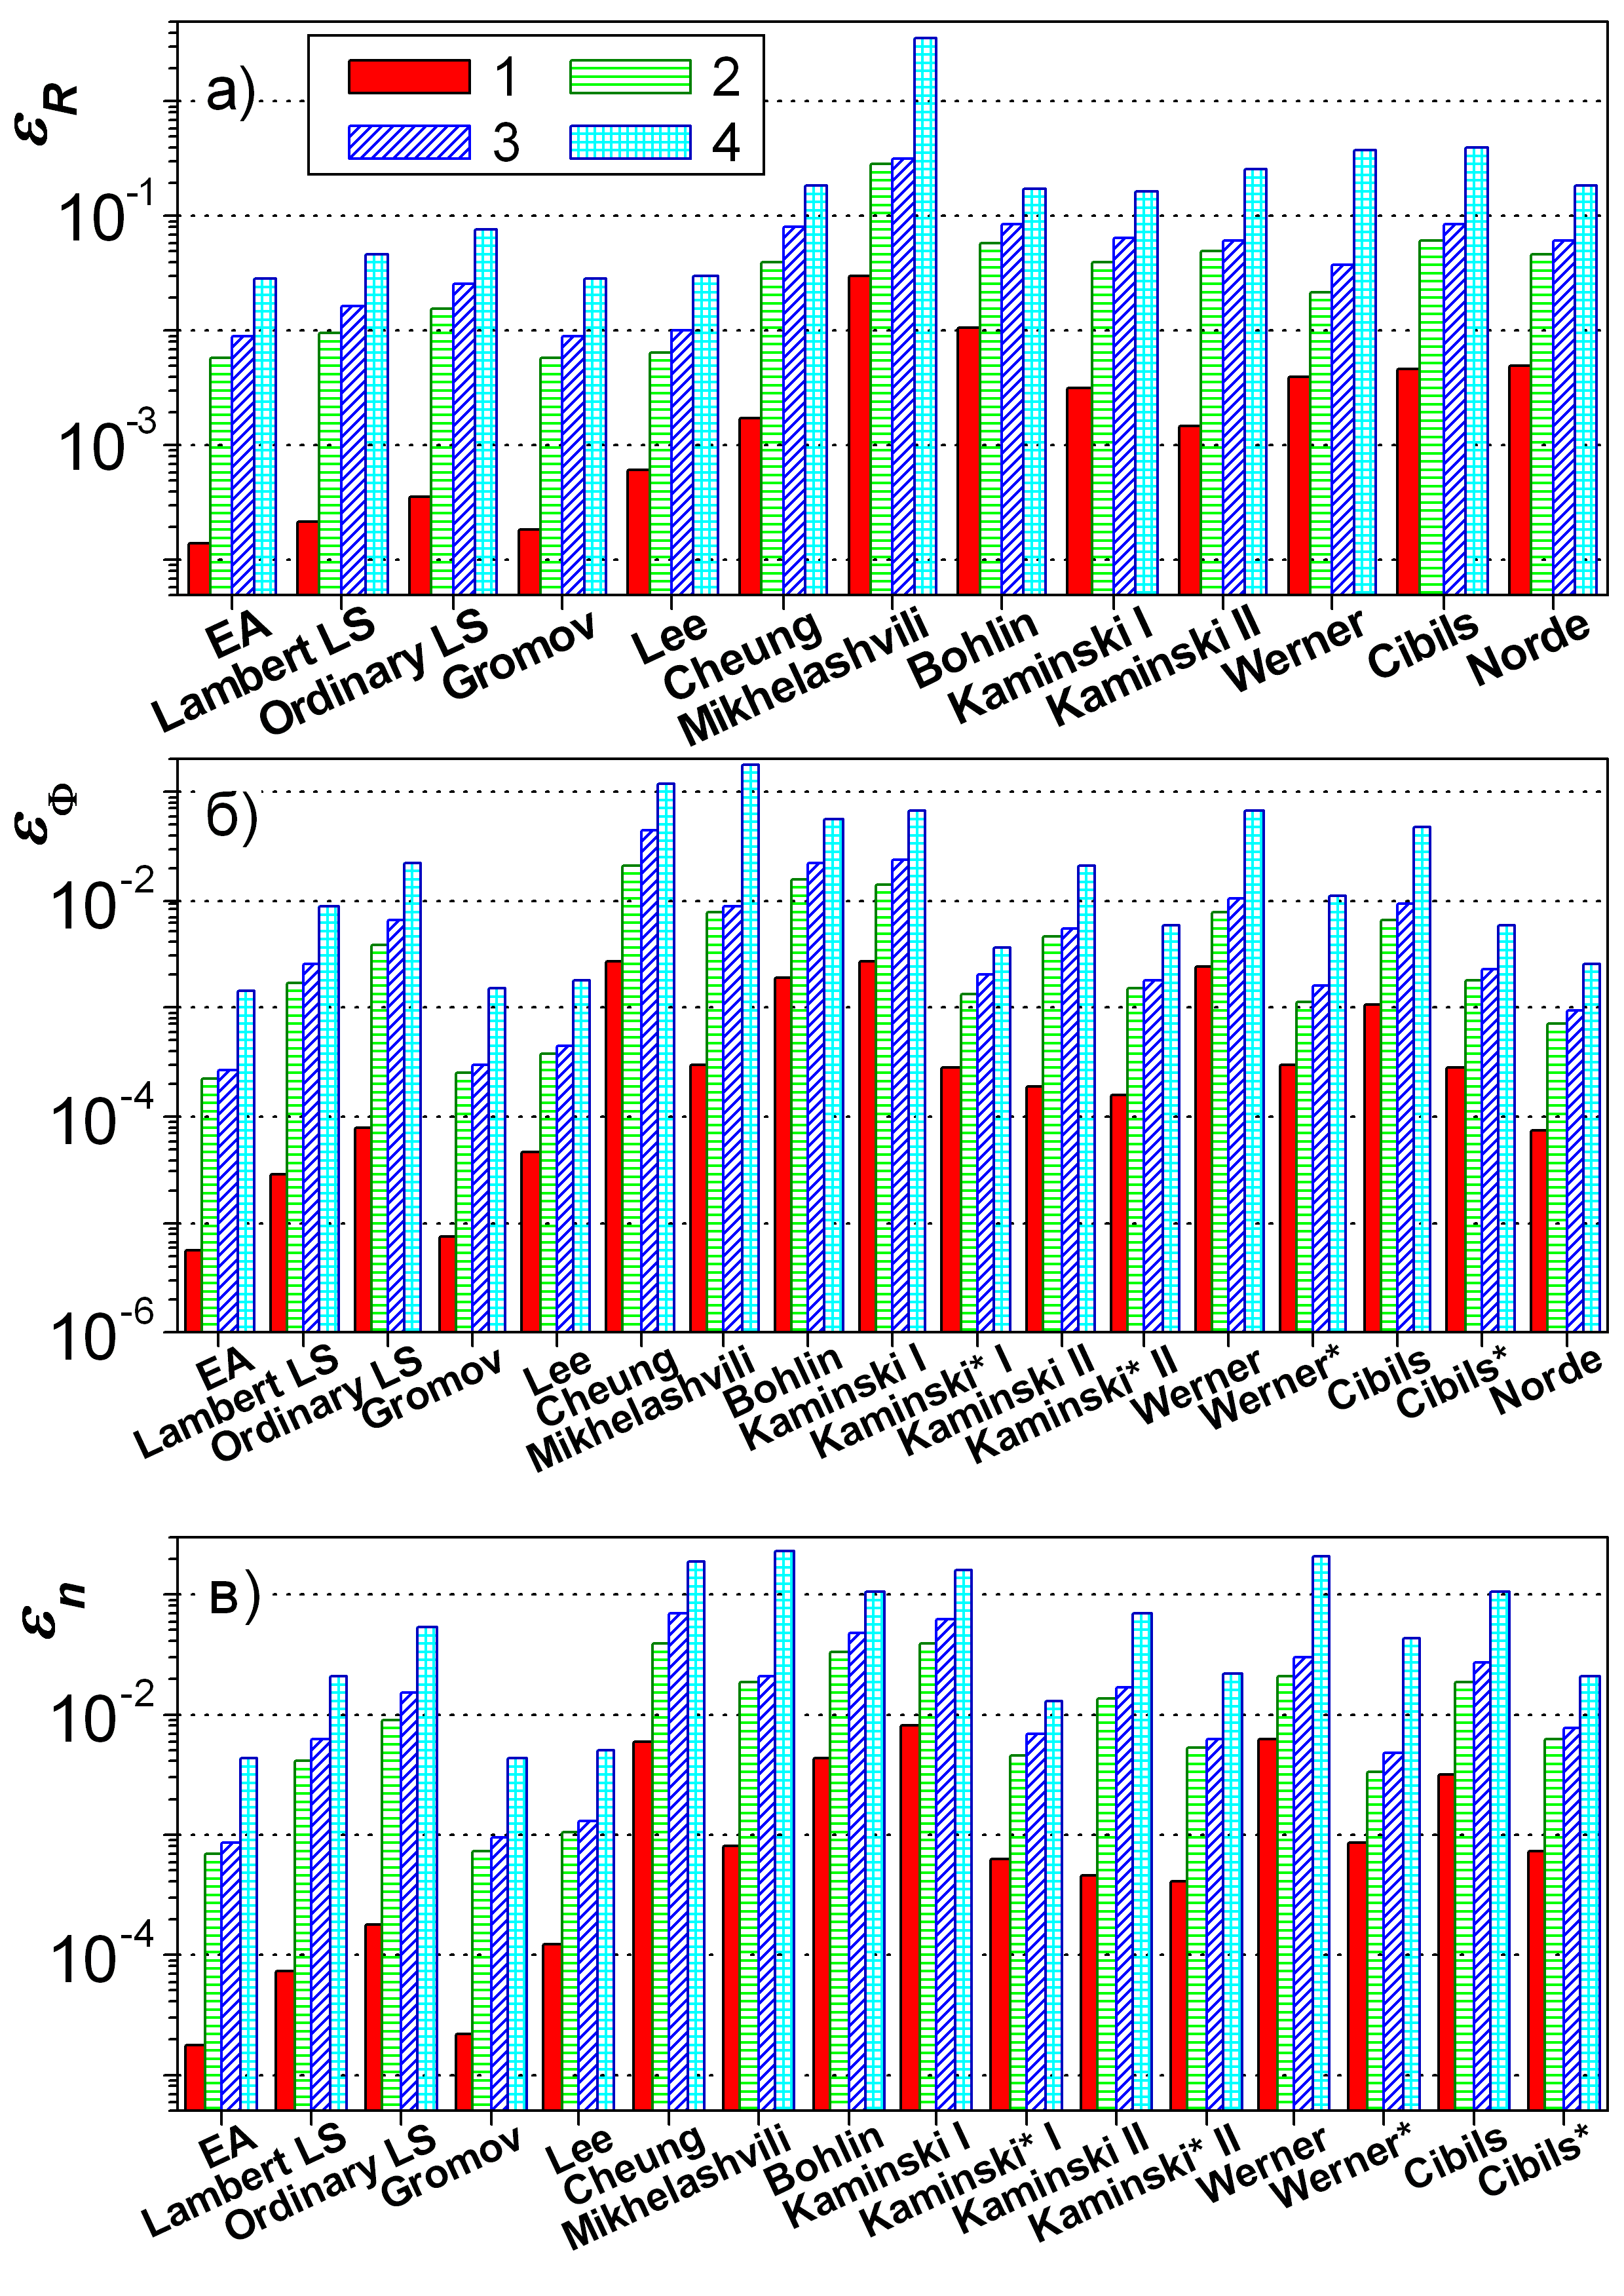
\includegraphics[width=0.8\textwidth]{figDiag}%
\caption{\label{figDiag}
Похибки визначення $R_s$ (a), $\Phi_b$ (б) та $n_\mathrm{id}$ (в) з наборів зашумлених даних.
$\sigma_V$, мВ: 0 (1), 0,3 (2, 3), 2 (4).
$\sigma_I^\varepsilon$, \%: 0 (1), 0,5 (2), 1 (3, 4).
}
\end{figure}


У випадку, коли методи Werner, Cibils, Kaminskii~I або  Kaminskii~IІ застосовуються до зашумлених даних, визначення $n_\mathrm{id}$ шляхом апроксимації скорегованої ВАХ є більш точним, ніж у випадку, коли ця величина визначається внаслідок апроксимації допоміжної функції.
Крім того, точність цих методів наближається до найкращих результатів інших методів і стає порівняною з точністю чисельних методів, або й навіть переважає її --- див. Рис.~\ref{figG1003}.
Метод Norde дозволяє достатньо точно визначати висоту бар'єру Шотки, проте фактор неідеальності можна отримати лише застосовуючи інші методи.

Залежності похибок визначення параметрів від рівня шуму (від рівня випадкових помилок) показані на Рис.~\ref{figErr}.
Наведені графіки отримані при використанні методу Gromov, проте вони є цілком типовими і для інших методів також.
Видно, що величини помилок при визначенні всіх параметрів практично лінійно залежать як від похибок вимірювання напруги, так і від відносних похибок сили струму.
Крім того, помилки визначення $\Phi_b$ та $n_\mathrm{id}$, викликані неточністю вимірювання напруги та сили струму, значно менші, ніж помилки визначення послідовного опору за тих самих умов.


\begin{figure}
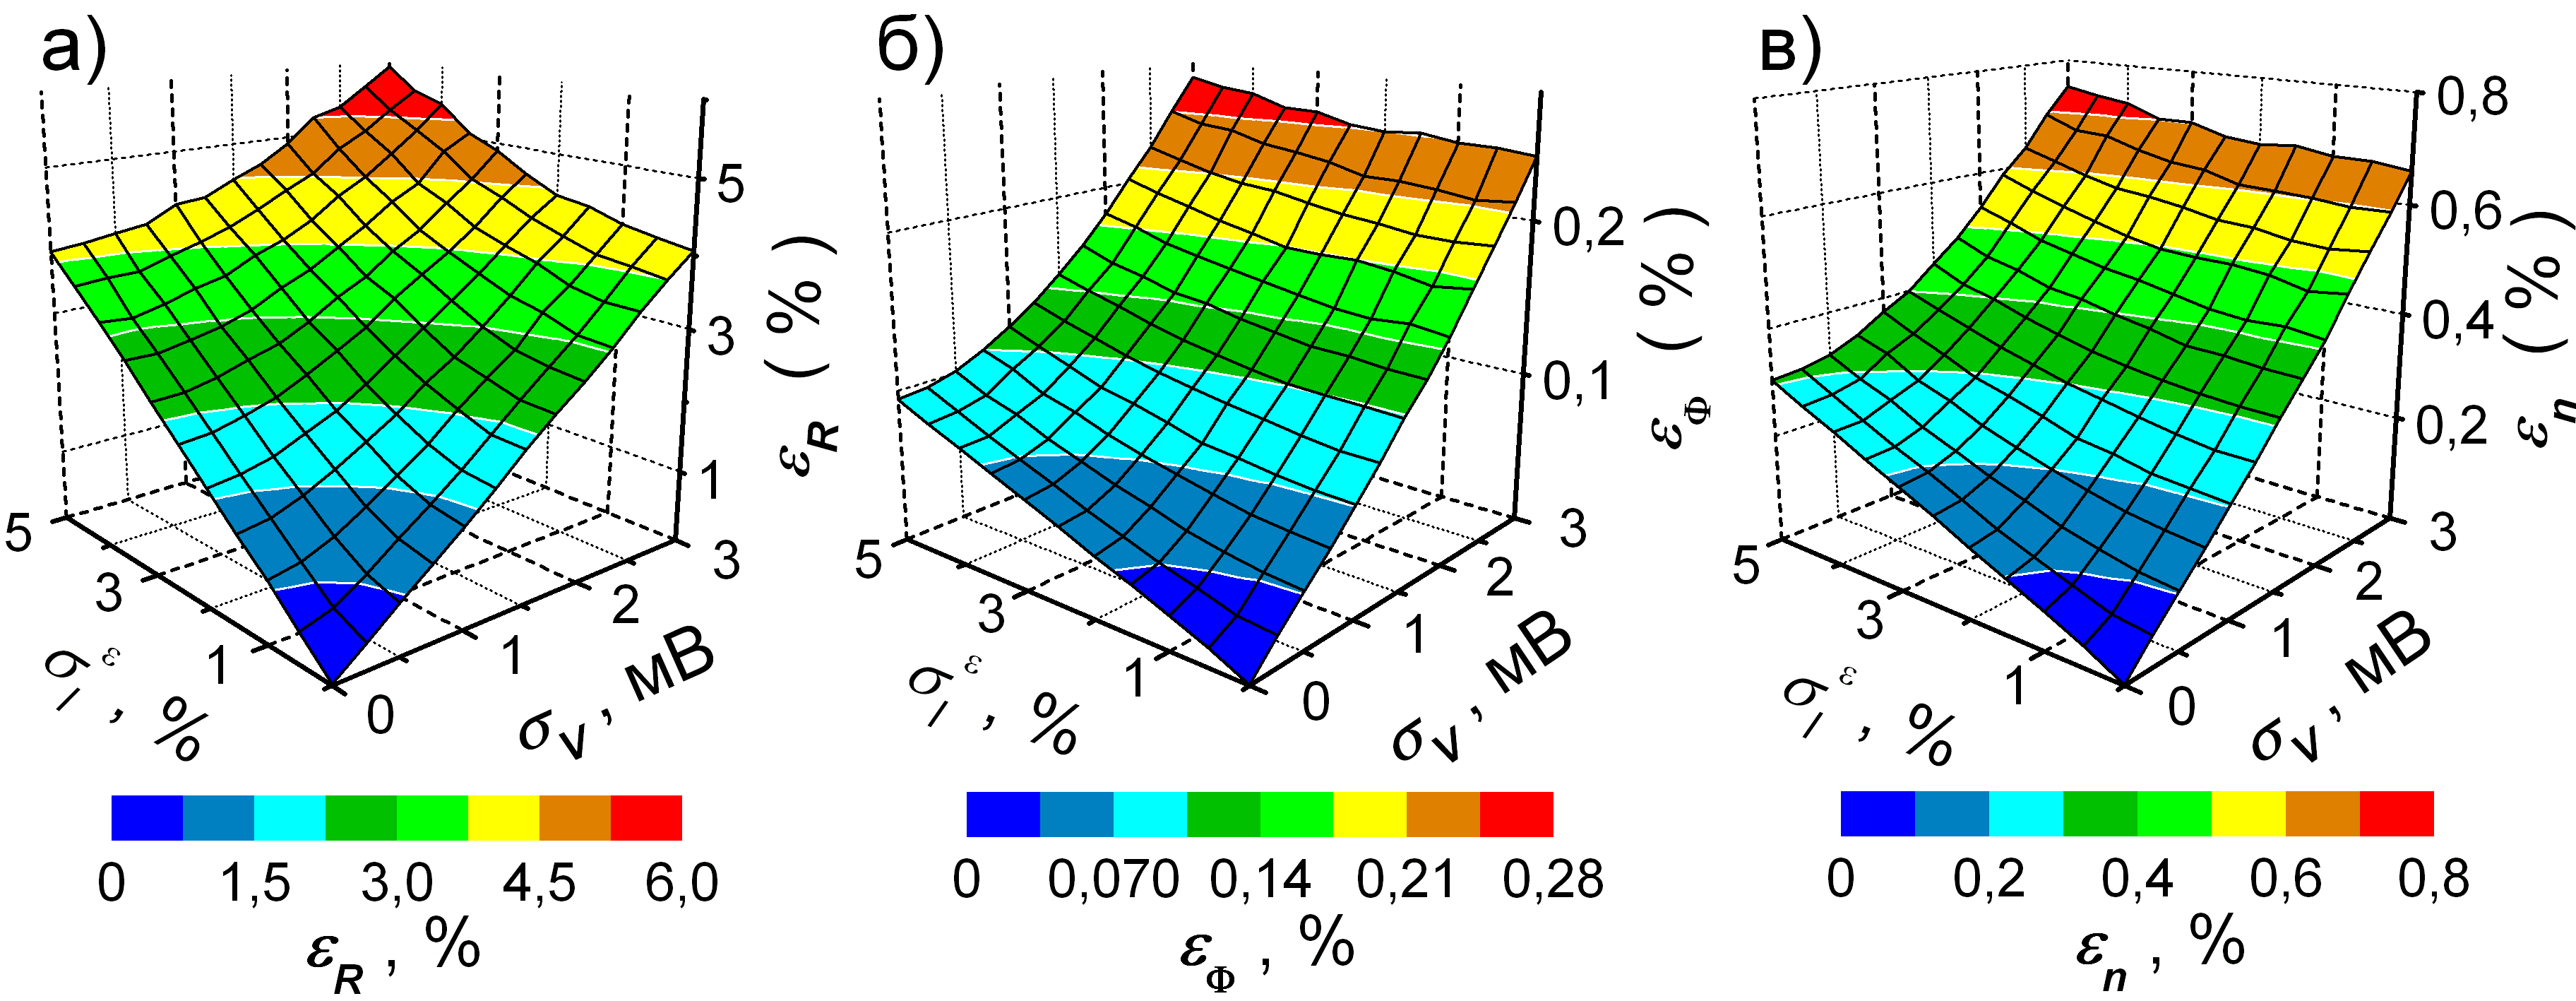
\includegraphics[width=1\textwidth]{figErr}%
\caption{\label{figErr}
Залежності похибок визначення $R_s$ (a), $\Phi_b$ (б) та $n_\mathrm{id}$ (в) при використанні методу Gromov  від похибок вимірювання сили струму та напруги.
}
\end{figure}


\subsection{Визначення параметрів реальних структур метал--напівпровідник}

Температурні залежності параметрів, отриманих з експериментальних ВАХ наведені на Рис.~\ref{figPract}.
Зауважимо, що в цьому випадку при застосуванні метода Bohlin були використані значення $\gamma_1=1,6$ та $\gamma_2=1,8$ замість  $\gamma_1=1,6$ та $\gamma_2=3,5$, для яких, як показано в розділі~\ref{AnMethod}, очікується менше значення похибки.
Це пов'язано з тим, що для діапазону сил струму, у якому були отримані експериментальні дані, відсутній мінімум функції Норда з $\gamma_N=3.5$.



\begin{figure}
\center
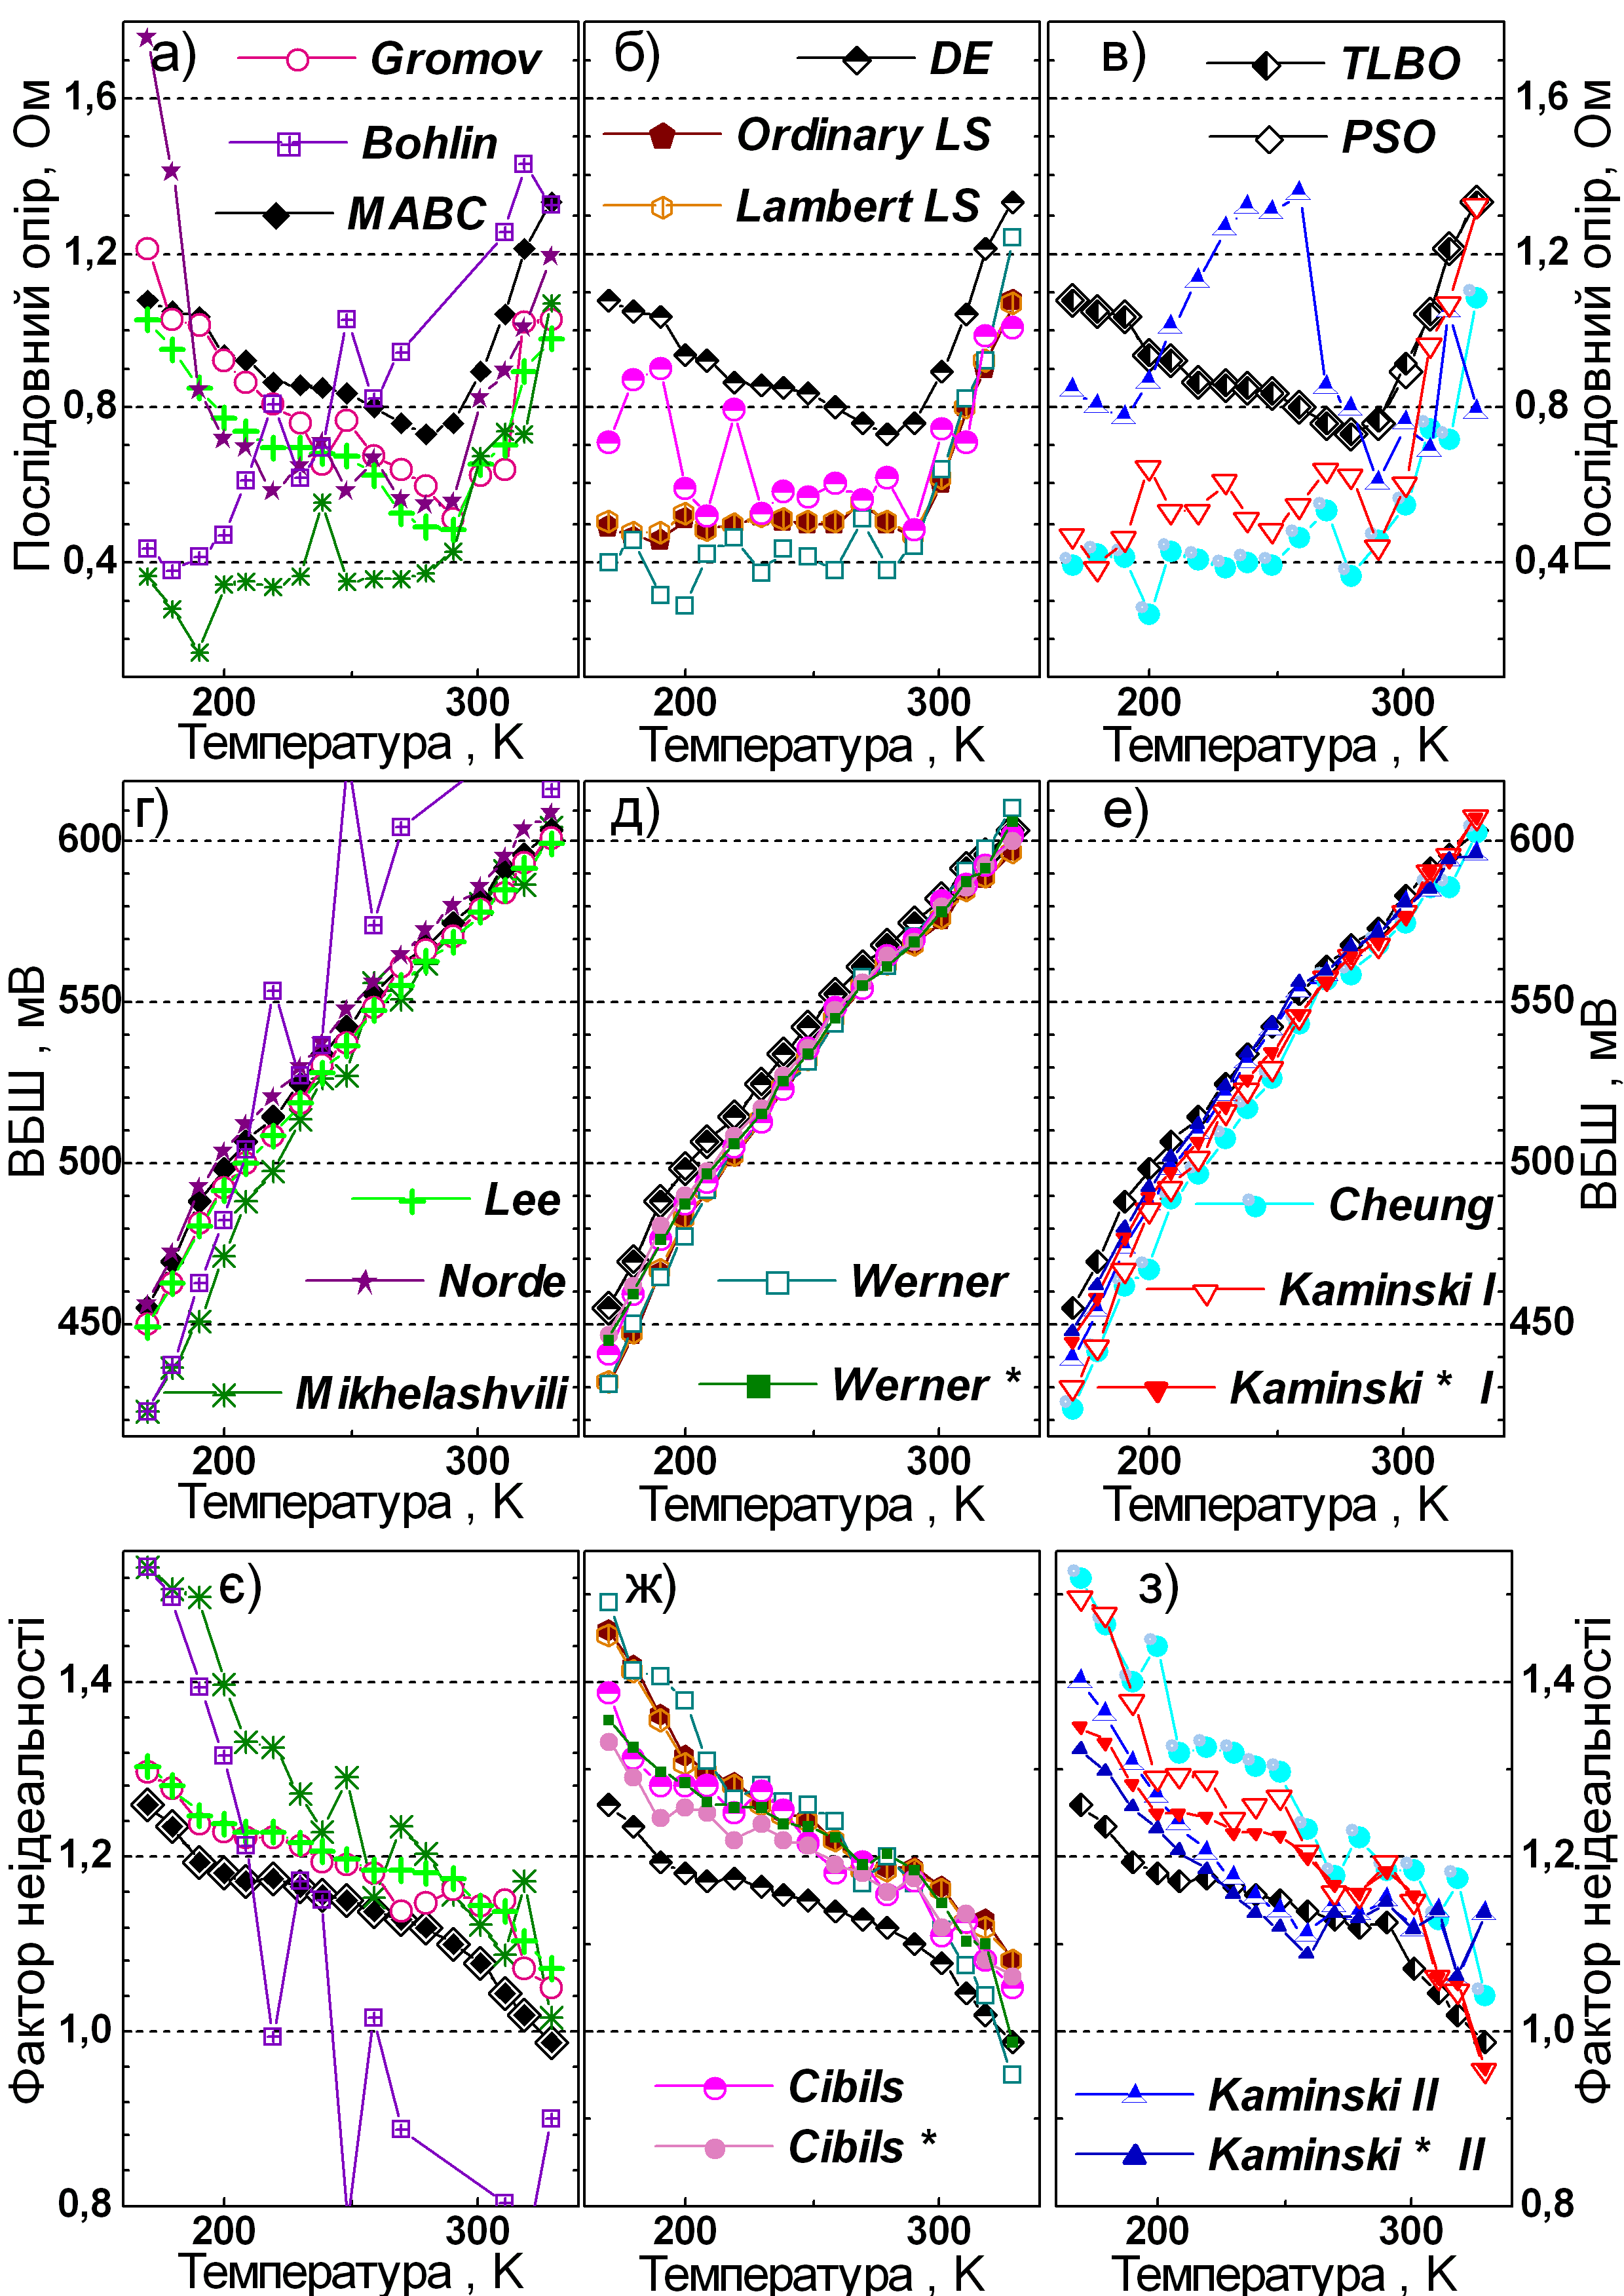
\includegraphics[width=0.8\textwidth]{figPract}%
\caption{\label{figPract}
Температурні залежності послідовного опору (а --- в), ВБШ (г --- е) та фактору неідеальності (є --- з) при
застосуванні різних методів до експериментальних ВАХ.
}
\end{figure}

Виявлена температурна залежність висоти бар'єру, які відрізняється від виразу (\ref{eqFbT}), що використовувався при синтезі ВАХ, може бути пов'язана з неоднорідністю контакту МН \cite{Tung:MSE,Olikh:2013IEEE}.
Зростання послідовного опору при високих температурах в літературі \cite{Rs:Dokme} пов'язується з тим, що за цих умов визначальним для $R_s$ буде контактний опір, а не опір об'єму напівпровідника.

Зупинимось на отриманих температурних залежностях послідовного опору.
Використання ЕА, методів Gromov та Lee дозволяє виявити немонотонну температурну залежність $R_s$, причому абсолютні значення опору, отримані за допомогою різних методів, дещо відрізняються.
Взявши до уваги невелике значення послідовного опору (близько 1~Ом), а також виявлене раніше значне збільшення похибок методів Gromov та Lee при малих значеннях $R_s$ та великих $I_s$ (див. Рис.~\ref{figId},a, \ref{figR3D},a, \ref{figR3D},б та \ref{figG1003},a), можна зробити висновок, що величини, отримані при застосуванні еволюційних алгоритмів, більш правильні.
З фізичної точки зору, виявлена поступова зміна опору з температурою є цілком ймовірною.
При застосуванні числових методів отримана залежність $R_s$ від $T$ також є досить гладкою, проте її поведінка відрізняється від результатів ЕА при низьких температурах (див. Рис.~\ref{figPract},б).
З іншого боку, зашумленість температурних залежностей має свідчити про наявність помилок або під час вимірювань ВАХ, або під час визначення параметрів, а саме такі залежності виникають при застосуванні інших методів.

Подібні особливості характерні і для визначених залежностей ВБШ та фактора неідеальності.
Розкид значень $\Phi_b$ суттєво менший ніж для $n_\mathrm{id}$, що корелює з меншою величиною похибки визначення ВБШ (див. Рис.~\ref{figG1003} -- \ref{figErr}).
Найбільш погані результати отримані при використанні методів Bohlin, Mikhelashvili та Cheung.

Для оцінки розходжень виміряних та апроксимуючих ВАХ було використане середнє значення відхилення сили струму $\Delta_I$:
 \begin{equation}
 \label{eqMCur}
 \Delta_I=\frac{1}{N_p}\sum_{i=1}^{N_p}\left|\frac{I_{calc}(V_i)-I_i}{I_i}\right|.
 \end{equation}
При обчисленні $\Delta_I$, значення $I_{calc}(V_i)$ розраховувалися з використанням виразів (\ref{eqSDIV}--\ref{eqSDIs}) та параметрів, визначених при використанні різних методів.
Результати для трьох ВАХ, виміряних при різних температурах, наведені на Рис.~\ref{figPrAcc}.
Як видно, в цьому випадку еволюційні алгоритми, методи Gromov та Lee також продемонстрували свої переваги.


\begin{figure}
\center
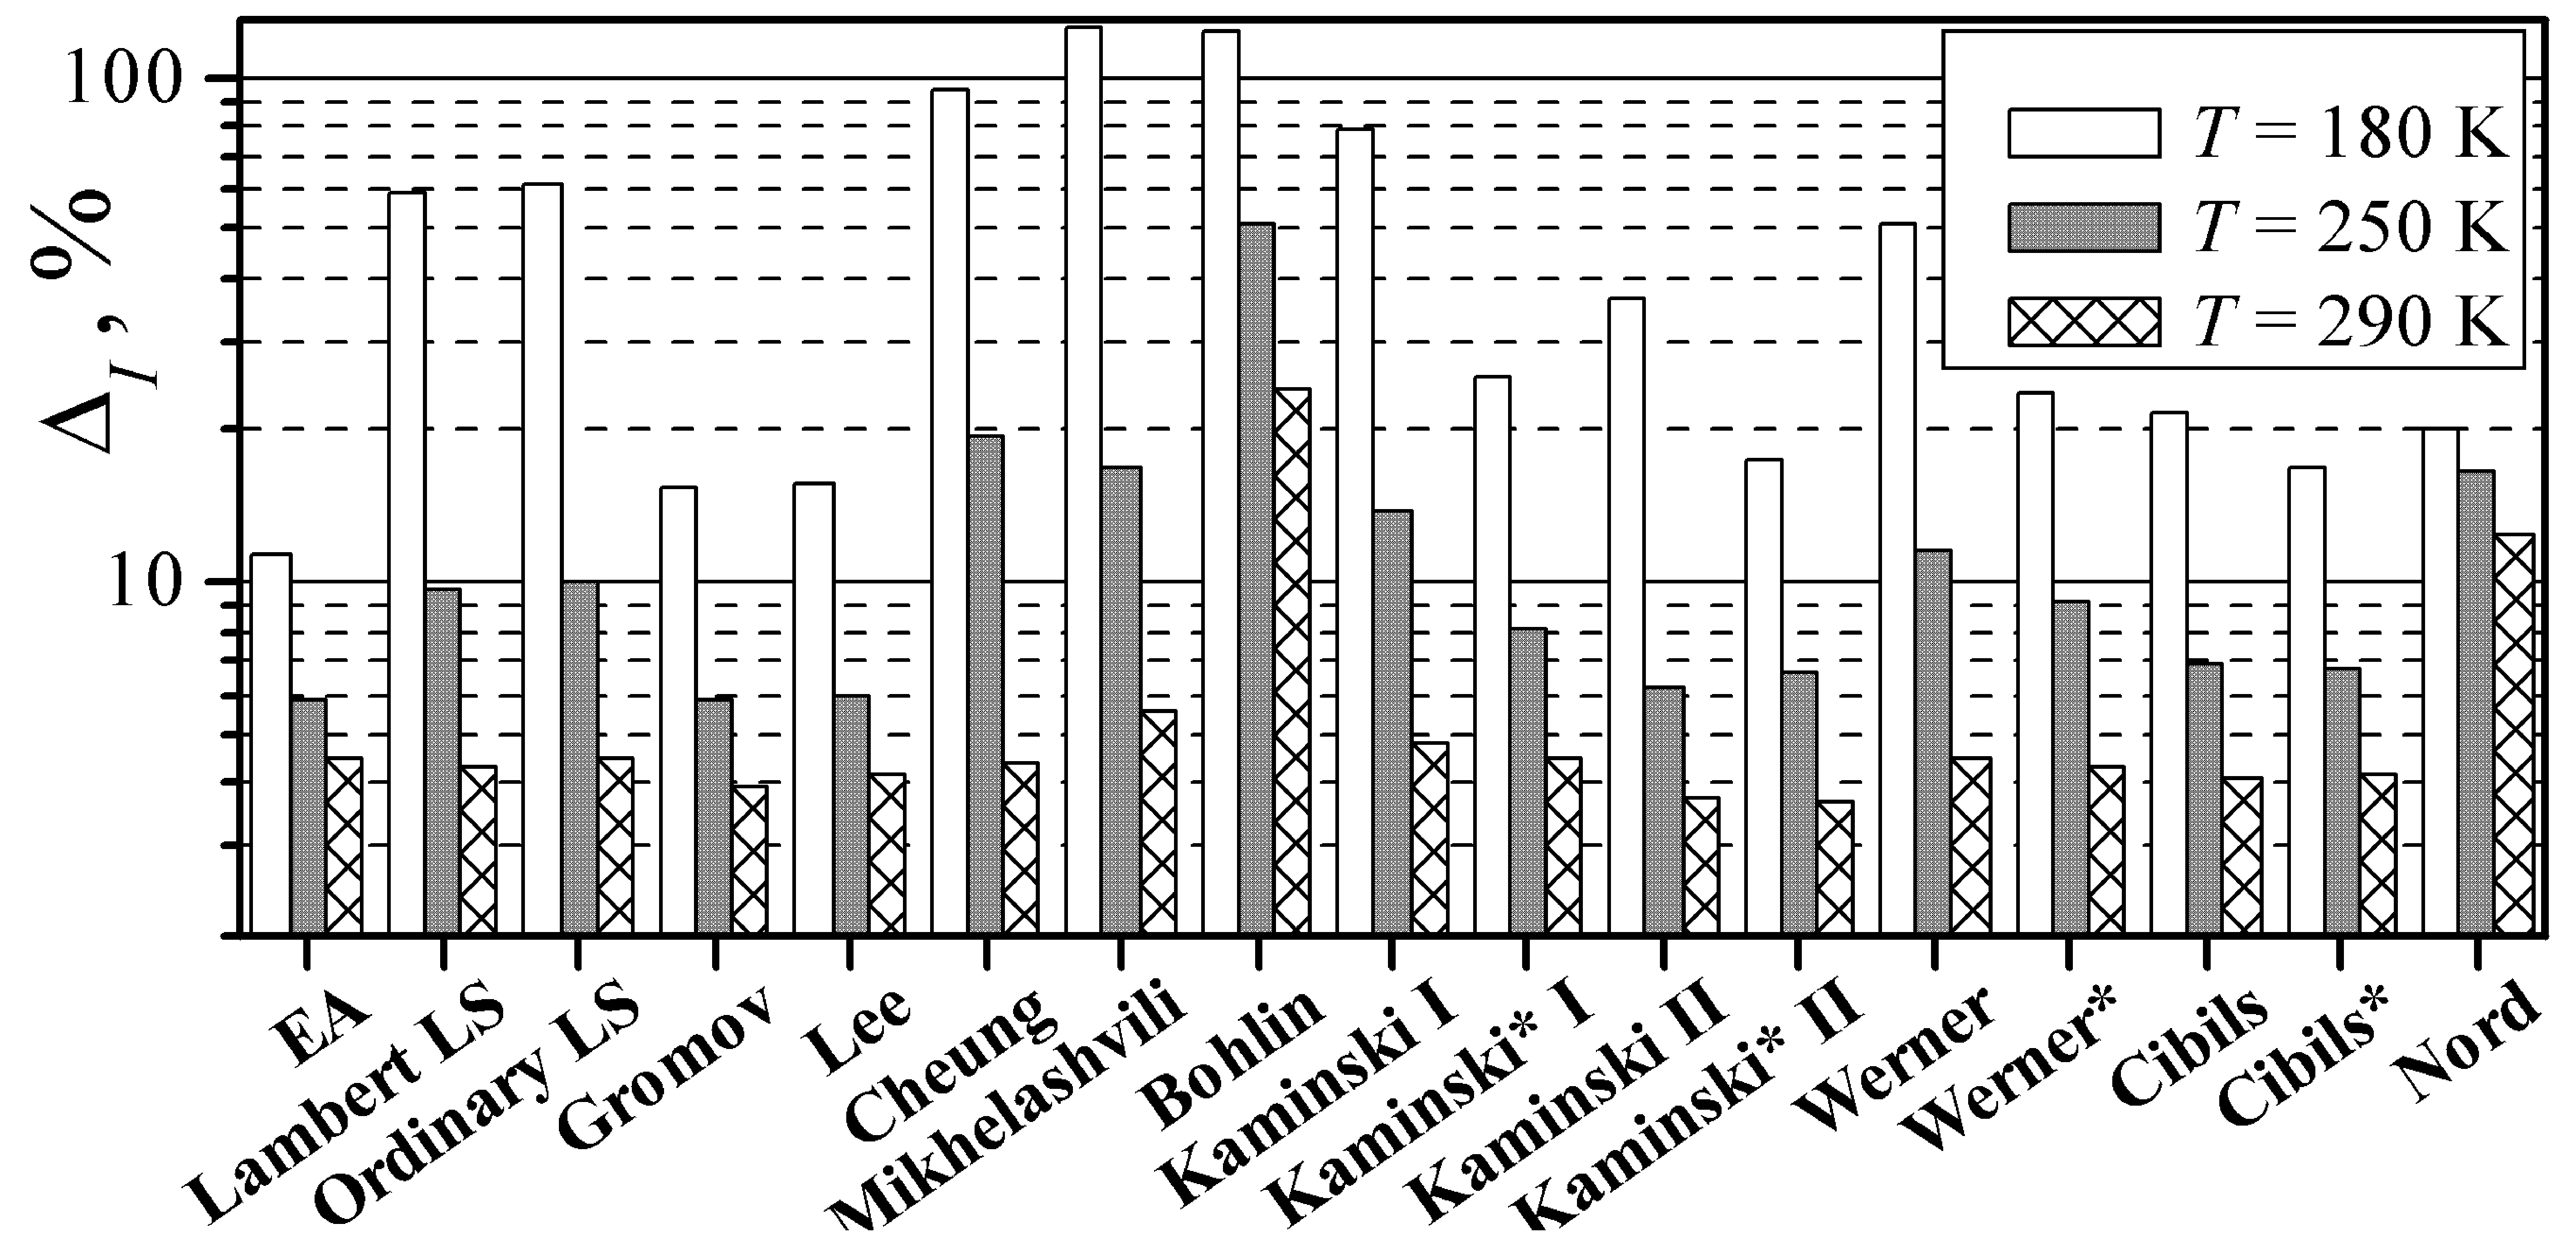
\includegraphics[width=0.8\textwidth]{figPrAcc}%
\caption{\label{figPrAcc}
Середні значення відносного відхилення розрахованих значень сили струму від експериментальних даних.
}
\end{figure}

Як було сказано раніше, і експериментальні ВАХ отримані для кремнієвих структур, і при синтезі даних вважалося, що ДШ створені з використанням саме цього напівпровідника.
На мою думку, висновки щодо того, які методи є найбільш достовірними та такими, що мають перевагу, залишаються справедливими і при дослідженні структур не на основі кремнію.
Дійсно, для діодів з іншого матеріалу можуть спостерігатися зміни  величин $\Phi_b$, $n_\mathrm{id}$, $R_s$ та їх співвідношень.
Проте еволюційні алгоритми, методи Lee та Gromov з адаптивною процедурою довели свою перевагу для досить широкого діапазону значень параметрів.
З іншого боку, зміна матеріалу може викликати модифікацію
а)~температурної залежності точності визначення параметрів;
б)~абсолютного значення похибки.
Проте подібні зміни для конкретного напівпровідника можуть бути у першому наближені оцінені з використанням даних, наведених у Таблиці~\ref{tabIF}.

Проте необхідно підкреслити, що отримані результати будуть коректними для тих ДШ, для яких ВАХ описуються рівнянням~(\ref{eqSDIV}).
Так, наприклад, відхилення від цього закону характеристик реальних діодів може бути пов'язане з наявністю шунтуючого опору чи неоднорідністю бар'єру \cite{Tung:MSE,OlikhJAP}.
Проте в подібних випадках застосування еволюційних алгоритмів може суттєво спростити процедуру визначення параметрів структур МН.


\section*{Висновки до розділу \ref{Ch_MSMethod}}
\addcontentsline{toc}{section}{Висновки до розділу \ref{Ch_MSMethod}}	
  \begin{enumerate}[leftmargin=0cm,itemindent=3em]
     \item Проведено порівняльний аналіз та тестування 16 основних відомих методів визначення параметрів діодів Шотки з вольт--амперних характеристик.
         Спираючись на результати тестування методів на експериментальних та синтезованих  ВАХ,
         запропоновано шляхи їх оптимізації з метою збільшення точності розрахунку.

     \item Для методу Норда проведено чисельний аналіз залежності величин похибок визначення ВБШ та послідовного опору в методі Норда від величини параметра $\gamma_N$ на масиві синтезованих ідеальних та зашумлених ВАХ.
     Виявлено, що похибка визначення висоти бар'ру зростає зі збільшенням даного параметру, тоді як залежність похибки розрахунку послідовного опору є немонотонною функцією $\gamma_N$.
     Показано, що оптимальним значенням є $\gamma_N=1,8$.


     \item Проведено чисельний аналіз залежності величин похибок визначення висоти бар'єру, фактору неідеальності та послідовного опору при використанні Bohlin--методу від величин параметрів $\gamma_1$ та $\gamma_2$.
     Встановлено, що в цьому методі похибка екстрагування параметрів зростає при збільшенні величини $|\gamma_1-\gamma_2|$.
     Запропоновані оптимальні (для температурного діапазону $130\div330$~К) величини $\gamma_1=1,6$ та $\gamma_2=3,5$.



     \item Для оптимізації вибору діапазону ВАХ, який використовується для побудови допоміжних функцій при застосуванні аналітичних методів визначення параметрів структур МН, запропоновано адаптивну процедуру, що базується на аналізі відхилення між апроксимуючою та експериментальною кривими.
         На прикладі аналітичного Gromov методу показано, що дана процедура дозволяє підвищити точність визначення параметрів (приблизно на порядок при кімнатних температурах у випадку низького рівня похибок вимірювання) і не викликає критичного збільшення часу, необхідного для розрахунків.

     \item Запропоновано модифікацію методу Mikhelashvili, яка дозволяє застосовувати його в автоматичному режимі до множини ВАХ.
     Вона полягає у послідовному використанні медіанного фільтру та процедури згладжування функції $\alpha(V)=d(\ln I)/d(\ln V)$ перед знаходженням положення її максимуму.
     Показано доцільність застосування запропонованої процедури при опрацюванні реальних ВАХ для підвищення точності методу, що пов'язано зі можливістю знаходження саме глобального екстремума.

    \item Здійснена програмна реалізація еволюційних алгоритмів  диференційної еволюції, оптимізації зграї частинок,
модифікованої штучної бджолиної сім'ї та оптимізованого викладання та навчання при вирішенні задачі визначення параметрів структур МН.
Запропоновано та показано ефективність застосування цільової функції у вигляді суми квадратів відносних похибок апроксимації кожної з точок ВАХ.
Проведено визначення необхідної кількості поколінь для збіжності кожного з алгоритмів.

   \item Показано, що серед всіх тестованих методів, найбільш придатними з точки зору точності визначення параметрів є еволюційні алгоритми (особливо MABC завдяки найменшому часу розрахунку), метод Gromov з адаптивною процедурою та метод Lee, причому ЕА дозволяють отримати найбільш коректні результати при малих (декілька Ом) значеннях послідовного опору або великих значеннях струму насичення (високих температурах).
    Показано, що використання функції Ламберта при чисельному визначенні параметрів ДШ дозволяє зменшити похибки визначення та вплив на них інших факторів; з іншого боку, час роботи алгоритму зростає.
    Проаналізовано залежності точностей визначення послідовного опору, висоти бар'єру Шотки та фактора неідельності від величин параметрів та рівня випадкових помилок вимірювання ВАХ.

  \end{enumerate}

Предсталені в даному розділі результати огляду, тестування та порівняльного аналізу методів визначення параметрів діодів Шотки будуть корисними для подальших дослідження та розробки
МН пристроїв.

Основні результати даного розділу представлені та використані в роботах \cite{Olikh:Rev,6CPFCS,OlikhJAP,Olikh:Ultras2016,Olikh2016JSem}.


\chapter{\MakeUppercase{Ефекти впливу} $\gamma$--\MakeUppercase{опромінення та ультразвукового навантаження при кімнатних температурах
на структури} Al$-n-n^+$--Si---Al \MakeUppercase{з контактом Шотткі}\label{Ch_GammaSD}}

Як відомо, структури метал--напівпровідник є основою для створення різноманітних польових транзисторів, детекторів високочастотного
випромінювання, сонячних елементів тощо;
діоди з контактом Шотткі широко використовуються під час виробництва високошвидкісних логічних, інтегральних та оптоелектронних елементів
і тому інтерес до подібних структур з боку науковців є цілком зрозумілим.
Одним з основних підходів для опису струму через контакт МН є теорія термоелектронної емісії (ТЕ),
згідно з якою \cite{Colinge,Sze2012,Rhoderick1988,StrihaBook} ВАХ має описуватися виразами (\ref{eqSDIV})--(\ref{eqSDIs}),
причому фактор неідеальності має бути рівний одиниці, послідовний опір нульовим,
а ВБШ визначається різницею між роботою виходу електрону з металу та енергією електронної спорідненості в напівпровіднику \cite{Colinge}.
Проте для реальних структур МН ці вирази нерідко є занадто спрощеними, оскільки
слід враховувати дію сил зображення, наявність проміжного діелектричного прошарку та електронних станів на границі розділу,
неоднорідність контакту, падіння прикладеної напруги не лише в області збідненого шару напівпровідника тощо.
Як наслідок, зокрема, величини $\Phi_b$ та $n_\mathrm{id}$ стають залежними від стану контакту та температури.
Окрім ТЕ, вірогідними причинами перенесення заряду в структурах МН є генераційно-рекомбінаційні процеси в області переходу,
різноманітні процеси витоку струму, тунелювання, термопольова емісія,
причому в двох останніх випадках суттєву роль можуть відігравати локальні енергетичні рівні тощо \cite{Rhoderick1988,Arslan,Donoval2010,Huang,Evstropov,VRH:Lee,Sathaiya}.
В результаті, сумарний струм часто розглядають у вигляді суми декількох доданків,
кожний з яких пов'язаний з окремим механізмом перенесення заряду і може бути домінуючим у своєму температурному чи польовому діапазоні \cite{Arslan,Donoval2010,Huang,GELCZUK2014}.
Зауважимо, що через суттєве різноманіття факторів впливу, задача про передбачення за певних
(у тому числі і температурних) умов механізму струмопереносу в структурах з бар'єром Шотткі є складною і такою, що не має загального вирішення.

З іншого боку, технічний розвиток передбачає розширення вимог до умов, в яких мають функціонувати напівпровідникові прилади.
Наприклад, подібні системи нерідко повинні функціонувати за умов різноманітного опромінення, наприклад, у космосі чи на атомних електростанціях.
Електрофізичні властивості структур МН дуже чутливі до стану границі розділу між металом та напівпровідником і будь--які
зовнішні фактори, що модифікують інтерфейс, суттєво впливають також і на властивості ДШ.
Радіаційне вплив є одним з таких факторів і тому вивчення впливу опромінення на характеристики МН структур є дуже важливим не лише завдяки
тому, що подібні дослідження дозволяють краще зрозуміти механізми та наслідки взаємодії радіації та твердого тіла,
але й через своє широке практичне застосування.


%years \cite{Kumar1, Rao, Kumar2, Sharma, Ohyama, Tataroglu, Tascioglu, Tataroglu2, Tataroglu3, Karatas, Umana, Kinoshita, Vorobets, Pattabi, Kovalyuk}.

Звичайно, подібним дослідження приділяється чимала увага  --- див., наприклад,
\cite{Kumar1, Rao, Kumar2, Sharma, Ohyama, Tataroglu,Tascioglu2010old,Tataroglu:2007NIMA,Tataroglu3,Karatas:2006NIMA,Umana,Kinoshita,Vorobets,Pattabi,Kovalyuk,Verma,Abdolahpour}.
Проте результати, отримані різними дослідниками, нерідко не збігаються.
Наприклад, було виявлено що ВБШ внаслідок радіаційного опромінення може як зменшуватися \cite{Kumar1, Rao, Kumar2, Sharma, Ohyama,Tataroglu3},
так і збільшуватися \cite{Tataroglu,Tascioglu2010old,Tataroglu:2007NIMA};
крім того, спостерігалися також ефекти немонотонної зміни висоти бар'єру при зміні дози опромінення \cite{Karatas:2006NIMA,Umana,Kinoshita,Vorobets, Pattabi, Kovalyuk,Verma}.
А отже, дане питання вимагає подальших досліджень.

Нарешті, незважаючи на достатньо широке експериментальне підтвердження можливості ефективного використання УЗ для впливу на властивості різноманітних напівпровідників та
пристроїв на їх основі
\cite{Bahar2003,ZobovFTP2008,Parchinskii2006r,Roman:2007APL,Roman:2010JAP,Zaver2005,Davletova2008,Teterkin2009r,Tagaev,Pashaev2012r,YOlikhTPL2011r,Zaveryukhin2002:2},
роботи, присвячені акустодинамічним явищам в ДШ, практично відсутні.
Таким чином, основна мета досліджень, результати яких представлені у даному розділі, полягала у наступному:
\begin{itemize}[leftmargin=0cm,itemindent=1em]
  \item З'ясування механізмів перенесення заряду  при прямому та
    зворотному зміщеннях у структурах Al$-n-n^+$--Si---Al, виготовлених стандартним промисловим способом при температурах, нижчих за номінальний робочий діапазон та поблизу кімнатних;
  \item Дослідження немонотонного впливу $\gamma$--опромінення на кремнієві ДШ;
  \item Вивчення впливу УЗН при кімнатній температурі на процеси перенесення заряду в МН--структурах на основі Si.
\end{itemize}



\section{Структури Al$-n-n^+$--Si---Al\label{MSSi}}

\begin{figure}[b]
\center
\includegraphics[width=0.5\textwidth]{MSSi}%
\caption{\label{figMSSi}
Структура зразків SSDA}
\end{figure}

%Для досліджень використовувалися діоди Шотткі з наступною структурою:
%на підкладці $n^+$-Si:Sb (KЭС~0.01, товщина 250~мкм) знаходиться епітаксійний шар $n$-Si:P (товщина 0.2~мкм);
%на поверхні епі-шару створено контакт  Шотки діаметром 2 мм шляхом нанесення шару молібдену;
%на протилежному боці підкладки --- омічний контакт.


В цьому розділі представлені результати дослідження діодів Шотткі Al$-n-n^+$--Si---Al,
виготовлених за стандартною технологією \cite{Vorobets:FM2003,StrihaBook1987} на пластинах кремнію КЭФ--1 товщиною $250$~мкм
з орієнтацією (111).
Пластини хімічно очищалися, з неробочої поверхні
повністю видалявся попередньо сформований шар SiO$_2$ для легування фосфором.
На робочій поверхні хімічним травленням створювалися вікна в SiO$_2$ і проводилося очищення
за допомогою іонного пучка.
Потім на робочу поверхню була напилена алюмінієва плівка і проводився процес фотолітографії.
Після цього на протилежну поверхню наносився шар алюмінію товщиною близько 1~мкм і проводився відпал
у інертній атмосфері.
Внаслідок термічної обробки утворювалася структура з випрямляючим контактом на робочій поверхні і омічним на протилежній.

Діаметр контакту Шотткі складав 2 мм (площа ДШ $A=3,14\cdot10^{-6}$~м$^2$).
Для контролю рівня легування приповерхневого шару були проведені
вимірювання вольт--фарадних характеристик (ВФХ) досліджуваних структур при кімнатній температурі ($T = 295$~К).
Приклад отриманої залежності наведено на рис.~\ref{figCV}.
Лінійність залежності $C^{-2}$ від $V$
(де $C$ --- ємність діоду Шотткі)
в широкому діапазоні зворотних напруг свідчить про рівномірність легування.
Виявлено, що концентрація носіїв заряду в приповерхневому шарі $N_d\approx1,2\cdot10^{23}$~м$^{-3}$.


\begin{figure}
\center
\includegraphics[width=0.7\textwidth]{figCV}
\caption{\label{figCV}
Залежність ємності Al$-n-n^+$--Si---Al діодів Шотткі $C$ (крива 1) та величини $C^{-2}$ (2) від прикладеної напруги.
$T=295$~К.
Точки --- експеримент, пряма --- лінійна апроксимація 2.
}%
\end{figure}







%В дисертації представлені результати, отримані з використанням кремнієвих ДШ двох типів,
%які ідентичних за структурою, проте відрізняються концентраціями концентраціями носіїв заряду в епітаксійному шарі $N_d$ та
%підкладці $N_s$, а також площею випрямляючого контакту $A$.
%Для контролю рівня легування були виконані вимірювання вольт--фарадних характеристик (ВФХ) досліджуваних структур при кімнатній температурі ($T = 295$~К).
%Параметри структур, а також їх позначення наведені в Таблиці~\ref{tabMSSi}.




Було проведено вимірювання ВАХ даних структур в діапазоні зміни постійного струму $(10^{-9}\div10^{-2})$~А при
прямому та зворотному зміщенні з кроком по напрузі 0.01~В в діапазоні температур $(130\div330)$~К.


\section{Особливості перенесення заряду в структурах Al$-n-n^+$--Si---Al з бар'єром Шотткі\label{MSSi_Non}}
\subsection{Перенесення заряду при прямому зміщенні\label{sbMSSi_NonF}}

%\subsubsection{Особливості аналізу експериментально виміряних ВАХ}

Приклади виміряних прямих ВАХ при різних температурах наведено на рис.~\ref{figIV_SDA}.
Видно, що при температурі більше 250~К прямі ВАХ в напівлогарифмічному масштабі є практично лінійними в інтервалі зміни струму близько трьох порядків.
В той самий час, при $T<210$~K загальний струм можна розділити на дві складові, причому для ВАХ, пов'язаної зі струмом,
який домінує при малих зміщеннях, суттєвим є вплив послідовного опору.
Про це свідчить відхилення від лінійності наведених кривих при при $7\cdot10^{-8}\mbox{A}<I<5\cdot10^{-7}\mbox{A}$.

В літературі \cite{Rhoderick1988,Gromov,Sze2012} показано, що в реальних структурах МН для опису залежності струму від прикладеної прямої напруги
навіть при врахуванні лише термоемісійних процесів замість виразу~(\ref{eqSDIV}) більш доцільно використовувати наступний
\begin{equation}
\label{eqSDIV:2}
I=I_s\exp\left[\frac{q(V-IR_S)}{n_\mathrm{id}kT}\right]\cdot
\left\{1-\exp\left[-\frac{q(V-IR_S)}{kT}\right]\right\}.
\end{equation}
У зв'язку з цим для опису прямих гілок ВАХ було використано вираз
\[
I=I_1+I_2=I_{s1}\exp{\left(\frac{qV}{n_{\mathrm{id},1}kT}\right)}\cdot
\left[1-\exp{\left(-\frac{qV}{kT}\right)}\right]+\]
\begin{equation} \label{eqSDA_IV}
+I_{s2}\exp\left[\frac{q(V-IR_S)}{n_{\mathrm{id},2}kT}\right]\cdot
\left\{1-\exp\left[-\frac{q(V-IR_S)}{kT}\right]\right\},
\end{equation}
де перший доданок $I_1$ є переважаючим при $I>10^{-5}$~A, а другий $I_2$ --- при $I<5\cdot10^{-7}$~A.
Використання двох доданків для опису ВАХ бар'єрних структур широко використовується
в літературі --- див., наприклад, \cite{Arslan,Donoval2010,Huang,GELCZUK2014}.
Зауважимо, що іншим поширеним методом врахування наявності особливостей на ВАХ при малих зміщеннях є введення шунтуючого опору, а не доданку $I_2$.
Проте, на нашу в думку, у даному випадку такий підхід не є виправданим, оскільки навіть при найменший зміщеннях пряма ділянка ВАХ не є лінійною --- див. вставку на рис.~\ref{figIV_SDA}.

\begin{figure}
\center
\includegraphics[width=0.8\textwidth]{figIV_SDA}
\caption{\label{figIV_SDA}
Прямі  ділянки ВАХ структур SSDA в температурному діапазоні $130\div330$~К.
Наведено криві, виміряні з кроком 20~К.
Лінії --- апроксимація прямої ВАХ при $T=130$~К за формулою~(\ref{eqSDA_IV}):
штрихова -- струм $I_1$, пунктирна -- $I_2$,
суцільна -- їх сума;
параметри апроксимації $n_{\mathrm{id},1}=1,67$,
$n_{\mathrm{id},2}=2,53$,
$I_{s1}=5,0\cdot10^{-13}$~A,
$I_{s2}=3,8\cdot10^{-10}$~A, $R_{s}=4.1\cdot10^3$~Ом.
На вставці --- початкова ділянка прямої ВАХ при $T=130$~K
}%
\end{figure}

Для визначення апроксимаційних параметрів використовувалася наступна процедура.
Пряма ВАХ розбивалася на дві ділянки,
для яких $10^{-5}\mbox{A}<I<10^{-2}\mbox{A}$ та
$10^{-9}\mbox{A}<I<10^{-7}\mbox{A}$.
Використовуючи дані першої, виконувалась побудова залежності величини $\ln{{I}/{\left[1-\exp\left(-qV/kT\right)\right]}}$ від $V$, яка надалі
апроксимувалася за методом найменших квадратів прямою,
кутовий коефіцієнт та вільний член якої пов'язані з $n_{\mathrm{id},1}$ та $I_{s1}$ відповідно.
Спираючись на дані другої ділянки ВАХ і використовуючи методи Cheung \cite{Cheung} та Gromov \cite{Gromov}, визначалась величина $R_s$.
Використання двох методів мало на меті підвищити достовірність отриманих даних і воно показало, що отримані обома шляхами значення близькі (в межах 10\%) між собою.
Після визначення $R_s$, будувалась залежність $\ln (I /\{1 - \exp[ -q (V - IR_s) / (kT ) ]\})$ від
ефективної напруги $(V-IR_s)$ і для визначення $I_{s2}$ та $n_{\mathrm{id},2}$ використовувалася процедура, описана вище.

На рис.~\ref{figIV_SDA} наведено приклад апроксимації експериментальної прямої ВАХ при одній з температур за формулою \eqref{eqSDA_IV} з використанням параметрів,
отриманих за описаною методою.
Видно задовільний збіг розрахованої кривої та експериментальних точок.

У випадку, коли проходження струму через бар'єр визначається ТЕ, то висота бар'єру Шотткі при
нульовому зміщенні $\Phi_b$ пов'язана зі струмом насичення співвідношенням \cite{Rhoderick1988}:
\begin{equation}
\label{eqFb:TE}
\Phi_b=\left(\frac{kT}{q}\right)\cdot\ln\left(\frac{AA^*T^2}{I_s}\right).
\end{equation}
Отримані температурні залежності для висот бар'єрів та факторів неідеальності обох компонент струму наведено на рис.~\ref{figFbT_SDA}.

%Розглянемо спочатку особливості струму, переважаючого при високих температурах та великих зміщеннях ($I_1$).


\begin{figure}
\center
\includegraphics[width=0.9\textwidth]{figFbT_SDA}
\caption{\label{figFbT_SDA}
Температурні залежності висоти бар'єру (а) та фактора неідеальності (б) структури SSDA.
1 -- $\Phi_{b1}$,
2 -- $\Phi_{b2}$,
3 -- $\Phi_{b1}^\mathrm{eff}$ ,
4 -- $n_{\mathrm{id},1}$, 5 -- $n_{\mathrm{id},2}$.
Пунктир -- лінійна апроксимація кривої 2.
Також приведено температурну залежність ширини забороненої зони Si (а, суцільна лінія)
}%
\end{figure}

З рисунка видно, що при збільшенні температури фактор неідеальності зменшується, наближаючись
до одиниці при кімнатних температурах.
Як відомо, що температурна залежність фактора неідеальності залежить від механізму перенесення заряду.
Зокрема, для ідеального випадку ТЕ очікується, що $n_{\mathrm{id}}=1$ при будь--яких температурах.
Проте для реальних контактів така рівність не спостерігається і для опису залежності $n_{\mathrm{id}}(T)$
часто використовують вираз \cite{Rhoderick1988, Sze2012}
\begin{equation}\label{eqN_T:TE}
n_{\mathrm{id}}=1+\frac{T_0}{T},
\end{equation}
де $T_0$ --- певна константа, що не залежить від температури та зміщення в широкому температурному інтервалі.

Проте залежність, подібна до зображеної на рис.~\ref{figFbT_SDA},б очікується
і у випадку, коли домінуючим механізмом є термопольова  емісія (ТПЕ), польова емісія (ПЕ) або тунелювання за участю глибоких рівнів (DAT)
\cite{Rhoderick1988,Evstropov,Soylu,JYOTHI2015,OZAVCI2013,Abhishek}.
В цьому випадку
\begin{equation}\label{eqN_T:TFE}
n_{\mathrm{id}}^\mathrm{T}=\frac{E_{00}}{kT}\cdot\coth\left(\frac{E_{00}}{kT}\right),
\end{equation}
де $E_{00}$ --- характеристична енергія тунелювання.


\begin{figure}
\center
\includegraphics[width=0.6\textwidth]{figNT_SDA}
\caption{\label{figNT_SDA}
Температурна залежність оберненого нахилу ВАХ.
1 --- $n_{\mathrm{id},1}$;
2 --- $n_{\mathrm{id},2}$.
Пунктир --- теоретичні криві відповідно до формул (\ref{eqN_T:TE}) (криві А та В)
та (\ref{eqN_T:TFE}) (криві С-G).
$T_0$, K: 12 (A), 206 (B).
$E_{00}$, мВ: 12 (С), 17 (D), 22 (E), 27 (F), 32 (G).
Також наведено ідеальний випадок ($n_{\mathrm{id}}=1$) --- пряма суцільна лінія
}%
\end{figure}

На рис.~\ref{figNT_SDA} наведено експериментально отримані залежності факторів неідеальності від оберненої температури
для обох струмових компонент та декілька кривих, розрахованих з використанням виразів (\ref{eqN_T:TE}) та (\ref{eqN_T:TFE}).
Видно, що отримані дані для $n_{\mathrm{id},1}$ (при $T>220$~K) та $n_{\mathrm{id},2}$ задовільно описуються
виразом (\ref{eqN_T:TE}) при $T_0=12$~К та $T_0=206$~К, відповідно,
що свідчить на користь ТЕ як основного механізму перенесення заряду.
Зауважимо, що при ТПЕ
\begin{equation}\label{eqE00:TFE}
E_{00}^\mathrm{TFE}=\frac{\hbar}{2}\sqrt{\frac{N_d}{m^*\varepsilon_s\varepsilon_0}},
\end{equation}
($m^*$ -- ефективна маса електрону, $m^*=1,08\cdot9,11\cdot10^{-31}$~кг)
і тому для досліджених зразків та температурного діапазону очікувалось, що при домінуванні цього механізму $n_\mathrm{id}\approx1$.



Раніше вже згадувалося, для однорідного контакту Шотткі теоретично \cite{Rhoderick1988} та експериментально \cite{Aboelfotoh,Zhua} показано,
що при підвищенні температури за умови домінування термоелектронної емісії ВБШ має зменшуватися,
причому температурні коефіцієнти змін $\Phi_b$ та  $E_g$ дуже близькі між собою.
На рис.~\ref{figFbT_SDA},а також наведена температурна залежність $E_g$, розрахована з використанням
виразу (\ref{eqEg}).
Для дослідженої структури спостерігається зворотна тенденція: ВБШ зі збільшенням температури зростає практично у всьому
діапазоні
і лише для компоненти $I_1$ поблизу кімнатної температури поведінка $\Phi_b$ нагадує $E_g$.

З іншого боку, відомо, що ВБШ, визначена за допомогою ВАХ, може відрізнятися від реальної.
Зокрема, в роботі \cite{Bozhkov} стверджується про необхідність проведення вимірів при сталому струмі через контакт
і пропонується для оцінки ефективної висоти бар'єру $\Phi_{b}^\mathrm{eff}$ використовувати вираз
\begin{equation}\label{eqBoz}
\Phi_{b}^\mathrm{eff}=n_{Ic}\Phi_b-(n_{Ic}-1)\cdot\frac{kT}{q}\cdot\ln\left(\frac{AA^*T^2}{I_c}\right),
\end{equation}
де
$n_{Ic}$ --- фактор неідеальності при певному сталому значенні струму $I_c$.
В роботі \cite{Bozhkov} також показано, що у випадку ТЕ через однорідний контакт $\Phi_{b}^\mathrm{eff}$ майже збігається за величиною
з реальною висотою бар'єру і має з нею однакову температурну залежність.

Результати обчислення $\Phi_{b1}^\mathrm{eff}$ для $I_{s1}$ згідно з формулою (\ref{eqBoz}) при $I_c=10^{-3}$~А показані на рис.~\ref{figFbT_SDA}, крива 3.
Видно, що хоча величина $\Phi_{b1}^\mathrm{eff}$ і змінюється в значно меншому діапазоні,
проте її температурна залежність також відрізняється від поведінки $E_g$, особливо при низьких температурах.


Якщо ТЕ є домінуючим механізмом перенесення заряду, то параметр $A^*$ може бути
визначений \cite{Rhoderick1988,Schroder2006} шляхом побудови так званої залежності Річардсона,
тобто залежності величини $\ln(I_s/T^2)$ від $(kT)^{-1}$.
Згідно з (\ref{eqFb:TE}) вона має описуватися виразом
\begin{equation}\label{eqRich}
\ln\left(\frac{I_s}{T^2}\right)=\ln(AA^*)-\frac{q\Phi_b}{kT},
\end{equation}
тобто залежність Річардсона має бути прямою, нахил якої визначається ВБШ,
я точка перетину з вертикальною віссю --- константою $A^*$.


Відповідна залежність, побудована для даних, отриманих для складової $I_1$ наведена
на рис.~\ref{figRich_SDA}, крива 1.
Видно, що лінійна залежність дійсно спостерігається, але не у всьому діапазоні температур, а у двох окремих піддіапазонах.
Шляхом апроксимації в діапазоні $(130\div220)$~К були отримані значення $3,7\cdot10^{-10}$~А$\cdot$см$^{-2}\cdot$К$^{-2}$ та
$0,141$~В для сталої Річардсона та висоти бар'єру, відповідно,
тоді як для діапазону $(230\div330)$~К ---
$30$~А$\cdot$см$^{-2}\cdot$К$^{-2}$ та $0,599$~В.
Величини також наведені в табл.~\ref{tabPar:SSDA}.
Очевидно, що отримані значення сталої Річардсона суттєво відрізняються від літературних даних
для кремнію (112~А$\cdot$см$^{-2}\cdot$К$^{-2}$).


\begin{figure}
\center
\includegraphics[width=0.7\textwidth]{figRich_SDA}
\caption{\label{figRich_SDA}
Залежності Річардсона, побудовані для високотемпературної компоненти струму $I_1$
за формулами (\ref{eqRich}) (крива 1) та (\ref{eqRichB}) (крива 2).
Прямі --- лінійна апроксимація даних кривої 1 в діапазонах $T=(130\div220)$~К (3, суцільна)
та $T=(230\div330)$~К (4, пунктир)
}%
\end{figure}



\begin{table}
\caption{\label{tabPar:SSDA}Параметри, визначені для високотемпературної складової струму неопромінених структур SSDA
}
\center
\begin{tabular}{|l|c|c|}
\hline
\multicolumn{1}{|c|}{Параметр:}& \multicolumn{2}{c|}{Температурний інтервал}\\ \cline{2-3}
метод визначення&$130\div220$~K&$230\div330$~K\\
\hline
%$A^*_R$, А$\cdot$см$^{-2}\cdot$К$^{-2}$&$3.7\cdot10^{-10}$&32\\ \hline
\multicolumn{1}{|c|}{$A^*$, А$\cdot$см$^{-2}\cdot$К$^{-2}$:}&&\\
залежність Річардсона (\ref{eqRich})&$(3,7\pm0,8)\cdot10^{-10}$&$32\pm10$\\
видозмінена залежність Річардсона (\ref{eqRichB})&$(3,0\pm0,6)\cdot10^{8}$&$40\pm8$\\
модифікована залежність Річардсона (\ref{eqRich:Mod})&$122\pm20$&$112\pm8$\\
література  \cite{Schroder2006}& \multicolumn{2}{c|}{$\,\,\,\,\,\,\,\,\,\,\,\,$   112}\\ \hline
\multicolumn{1}{|c|}{$\Phi_b$, мВ:}&&\\
залежність Річардсона (\ref{eqRich})&141$\pm$4&599$\pm$3\\
видозмінена залежність Річардсона (\ref{eqRichB})&1090$\pm$10&751$\pm$5\\
залежність $\Phi_b=f(\frac{1}{2kT})$&872$\pm$4&663$\pm$3\\
залежність $\Phi_b=f(n_\mathrm{id})$&646$\pm$5&640$\pm$20\\
модифікована залежність Річардсона (\ref{eqRich:Mod})&872$\pm$3&662$\pm$3\\
ВФХ &&683$\pm$2\\
\hline
залежність $\Phi_b=f(\frac{1}{2kT})$:&&\\
\multicolumn{1}{|c|}{$\sigma_{\Phi0}$, мВ} &99$\pm$1&40$\pm$5\\
\multicolumn{1}{|c|}{$\rho_2$, $10^{-2}$} &33$\pm$1&12$\pm$1\\
\multicolumn{1}{|c|}{$\rho_3$, мВ }&17,0$\pm$0,3&8,0$\pm$0,3\\
\hline
\end{tabular}
\end{table}



У роботі \cite{Aldemir} показано, що
У випадку суттєвого відхилення від ідеальності (величина $n_\mathrm{id}$ значно більша за одиницю)
для визначення $A^*$ можна також використовувати \cite{Aldemir,Mohan} видозмінену залежність Річардсона,
відкладаючи по осі абсцис не $(kT)^{-1}$, а $(n_\mathrm{id} kT)^{-1}$:
\begin{equation}\label{eqRichB}
\ln\left(\frac{I_s}{T^2}\right)=\ln(AA^*)-\frac{q\Phi_b}{n_\mathrm{id}kT},
\end{equation}
Проте для нашого випадку і видозмінена залежність Річардсона (рис.~\ref{figRich_SDA}, крива 2) не є лінійною для всього
температурного діапазону, а отримані значення $A^*$ (табл.~\ref{tabPar:SSDA}) суттєво відрізняються
від табличних.

Узагальнюючи вищенаведене, необхідно визнати, що отримані результати неможливо пояснити з точки зору теорії ТЕ через однорідний контакт.


З іншого боку, відмінності між експериментально виявленою температурною залежністю ВБШ та очікуваною теоретично нерідко
пов'язують із неоднорідністю границі розділу між металом та напівпровідником \cite{Dokme}.
Впливу неоднорідності можна позбутися розглядаючи ВБШ за умови плоских зон (<<flat band condition>>) $\Phi_{b}^\mathrm{FB}$:
\begin{equation}
\label{eqFbfb}
\Phi_{b}^\mathrm{FB}=n_\mathrm{id}\Phi_{b}-(n_\mathrm{id}-1)V_n\,,
\end{equation}
де
\begin{equation}
\label{eqVn}
qV_n=kT\ln\left(\frac{N_c}{N_d}\right)
\end{equation}
різниця енергій між дном зони провідності та положенням рівня Фермі в об'ємі напівпровідника,
так званий <<bulk potential>>.
На рис.~\ref{figFbfb_SDA} наведена температурна залежність $\Phi_{b}^\mathrm{FB}$, розрахована для високотемпературної компоненти $I_1$.
Зауважимо, що на рисунку також наведена температурна залежність ширини забороненої зони, причому
масштаби осей $\Phi_{b}^\mathrm{FB}$ та $E_g$ однакові.
З рисунка видно, що поведінка ВБШ в наближенні плоских зон та ширини забороненої зони дуже подібні,
що свідчить про те, що механізмом перенесення заряду в досліджуваних структурах може бути ТЕ через неоднорідний бар'єр.


\begin{figure}
\center
\includegraphics[width=0.55\textwidth]{figFbfb_SDA}
\caption{\label{figFbfb_SDA}
Температурні залежності ВБШ в наближені плоских зон (точки, права вісь), розрахованої
для високотемпературної компоненти струму $I_1$, та ширина забороненої зони (пунктир, ліва вісь)
}%
\end{figure}

В літературі для пояснення експериментально отриманих ВАХ структур МН використовуються два
підходи \cite{Sarpatwari, Tascioglu2010, Yildirim2010, Mamor, Iucolano2007JAP, Iucolano2007APL}, які дозволяють
%\cite{Sarpatwari, Aydemir, Turut, Mamor, Iucolano, Iucolano2}.
врахувати неоднорідність бар'ру Шотткі,
схематично ілюстровані за допомогою рис.~\ref{figFbModel}.
Згідно з першим підходом, запропонованим в \cite{Werner}, вважається, що контакт між металом та напівпровідником
змінюються від точки до точки (рис.~\ref{figFbModel},а),  просторовий розподіл ВБШ  може бути описаний розподілом Гауса:
\begin{equation}\label{eqFbWerner}
  P(\Phi_{b}^j)=\frac{1}{\sigma_\Phi\sqrt{2\pi}}\exp\left[-\frac{(\Phi_{b}^j-\overline{\Phi}_{b})^2}{2\sigma_\Phi^2}\right]\,,
\end{equation}
де
$P(\Phi_{b}^j)$ --- ймовірність того, що значення висоти бар'єру в певній точці дорівнює $\Phi_{b}^j$,
$\overline{\Phi}_{b}$ --- середнє значення ВБШ,
$\sigma_\Phi$ --- стандартне відхилення висоти бар'єру, показник однорідності контакту.
Також вважається, що $\overline{\Phi}_{b}$ та $\sigma_\Phi$ залежать
від прикладеної напруги і польова залежність може бути описана лінійними функціями
\begin{equation}\label{eqFbV}
   \overline{\Phi}_{b}(V)=\Phi_{b}^0+\rho_2\,V\,,
\end{equation}
\begin{equation}\label{eqNV}
   \sigma_\Phi^2(V)=\sigma_{\Phi0}^2+\rho_3\,V\,,
\end{equation}
де
$\Phi_{b}^0$ та $\sigma_{\Phi0}$ відповідають нульовому зміщенню,
а коефіцієнти $\rho_2$ та $\rho_3$ описують зміну розподілу ВБШ при прикладанні напруги.

\begin{figure}
\center
\includegraphics[width=0.9\textwidth]{figFbModel}
\caption{\label{figFbModel}
Моделі неоднорідного по площі контакту МН:
а --- ВБШ визначається розподілом Гауса;
б --- однорідний бар'єр з патчами
}%
\end{figure}

Ця теорія передбачає,
що фактор неідеальності, який визначається за нахилом ВАХ, і ВБШ, розрахована за допомогою виразу (\ref{eqFb:TE}),
пов'язані з $\rho_2$ та $\rho_3$ і
$\Phi_{b}^0$ та $\sigma_{\Phi0}$, відповідно \cite{Werner,Tascioglu2010,Yildirim2010,Mamor,Soylu}:
\begin{equation}\label{eqNidT}
  \frac{1}{n_\mathrm{id}}-1=\rho_2+\frac{q\rho_3}{2kT}\,,
\end{equation}
\begin{equation}\label{eqFb0T}
\Phi_b=\Phi_b^0-\frac{q\sigma^2_{\Phi0}}{2kT}.
\end{equation}

Відповідно до іншої моделі неоднорідного контакту Шотткі \cite{Sullivan,Tung:PhysRev,Tung:MSE,Tung:ApplPhysRev}, ВБШ вважається однаковою на всій границі МН,
окрім невеликих за площею ділянок (так званих патчів), де значення ВБШ менше --- рис.~\ref{figFbModel},б.
Ділянки можуть відрізнятися між собою площею та висотою бар'єру, причому відповідний характерний параметр описується розподілом Гауса.

В ряді робіт \cite{Iucolano2007JAP, Iucolano2007APL} показано, що ці теорії можуть бути використані сумісно,
причому за наявності патчів також має виконуватися співвідношення (\ref{eqFb0T}),
причому величина $\Phi_b^0$ має зміст ВБШ за межами патчів (в однорідній області),
а $\sigma_{\Phi0}$ пов'язаний з розподілом параметрів патчів:
\begin{equation}\label{eqGigFSigG}
  \sigma_{\Phi0}=\sigma_{\gamma p}\left(\frac{qV_{bb}N_d}{\varepsilon\varepsilon_0}\right)^{1/3},
\end{equation}
де
$\sigma_{\gamma p}$ --- стандартне відхилення для сукупності патчів параметра $\gamma_p$, який
характеризує окремий патч:
\begin{equation}\label{eqGammaP}
  \gamma_p=3\left(\frac{R_p^2\Delta_p}{4}\right)^{1/3},
\end{equation}
$\Delta_p$ та $R_p$ --- зниження висоти бар'єру в області патча та його розмір, відповідно.
Крім того, показано \cite{Sullivan,Tung:PhysRev,Iucolano2007JAP, Iucolano2007APL}, що за наявності неоднакових патчів
температурна залежність фактора неідеальності має описуватися виразом (\ref{eqN_T:TE}), причому
\begin{equation} \label{eqN_T0}
T_0=\frac{q\sigma_{\Phi0}^2}{3kV_{bb}}\,,
\end{equation}
де
$V_{bb}=(\Phi_b^0-V_n-V)$ --- вигин зон напівпровідника поблизу контакту.

Зауважимо, що підхід, який передбачає  врахування неоднорідності
інтерфейсної границі дуже широко використовується  для аналізу ВАХ різноманітних структур з контактом Шотткі
\cite{Soylu,GELCZUK2014,Mohan,JYOTHI2015,DURMUS2014,KHURE2015,OZAVCI2013,Cetin2005,Karatas:2006NIMA,Sarpatwari,
Tascioglu2010,Yildirim2010,Mamor,Iucolano2007JAP,Iucolano2007APL,Li2016}.

Залежності, побудовані відповідно до виразів (\ref{eqNidT}) та (\ref{eqFb0T}) наведені на рис.\ref{figFbNT1_SDA}.
Видно, що дійсно спостерігається лінійна залежність,
правда в двох окремих температурних діапазонах $T=(130\div220)$~К та $T=(230\div330)$~К.
Визначені шляхом лінійної апроксимації величини $\Phi_{b}^0$, $\sigma_{\Phi0}$, $\rho_2$ та $\rho_3$ для кожного з діапазонів
наведено в табл.~\ref{tabPar:SSDA}.

\begin{figure}
\center
\includegraphics[width=0.55\textwidth]{figFbNT1_SDA}
\caption{\label{figFbNT1_SDA}
Залежності величин $\Phi_{b1}$ (крива 1) та $n_{\mathrm{id},1}^{-1}-1$ (крива 2) від оберненої температури.
Прямі --- лінійна апроксимація у діапазонах $T=(130\div220)$~К (суцільна) та $T=(230\div330)$~К (пунктир)
}%
\end{figure}

Використовуючи вираз (\ref{eqN_T0}) та значення $\Phi_{b}^0\simeq0.663$~В, $\sigma_{\Phi0}\simeq0.04$~В
була розраховане значення $T_{0,teor}\approx11$~К, яке очікується в рамках моделі контакту Шотткі з локальними неоднорідностями
для температурного діапазону $(230\div330)$~К.
Ця величина досить близька до значення $T_{0,exp}\approx12$~К, отриманого експериментально (рис.~\ref{figNT_SDA}) у цьому ж діапазоні.
Ще одним аргументом на користь того, що струм $I_1$ може бути описаний в рамках моделі ТЕ через неоднорідний контакт є якісний збіг
поведінки $n_{\mathrm{id},1}$ при низьких температурах (рис.~\ref{figNT_SDA}) з очікуваною теоретично (\cite[Fig.11(b)]{Tung:PhysRev}).


У роботах  \cite{Tung:PhysRev,Sarpatwari,Schmitsdorf} показано, що для випадку
контакту з локальними неоднорідностями залежність між отриманими з аналізу ВАХ величинами $\Phi_b$ та $n_\mathrm{id}$ має бути лінійною,
причому $\Phi_{b}^0=\Phi_{b}+\Delta\Phi_b^\mathrm{IF}$ при $n=n_\mathrm{id}^\mathrm{IF}$
де $n_\mathrm{id}^\mathrm{IF}$ ---  величина фактора неідеальності з врахуванням впливу сил зображення,
$\Delta\Phi_b^\mathrm{IF}$ --- зниження бар'єру внаслідок дії сил зображення,
згідно з \cite{Sarpatwari}
\begin{equation}\label{eqN:IF}
n_\mathrm{id}^\mathrm{IF}\approx 1+\frac14\left[\frac{q^3N_d}{8\pi^2\varepsilon^2\varepsilon_0^2V^3_{bb}}\right]^{1/4},
\end{equation}
\begin{equation}\label{eqFb:IF}
\Delta\Phi_b^\mathrm{IF}\approx \left(\frac{q^3N_d\,V_{bb}}{8\pi^2\varepsilon^2\varepsilon_0^2}\right)^{1/4}.
\end{equation}
На залежності $\Phi_{b1}$ від $n_{\mathrm{id},1}$ (рис.~\ref{figFbN_SDA}), як і в попередній випадках,
спостерігаються дві лінійні області зі зламом при $T\sim225$~К.
Шляхом екстраполяції отримано, що $\Phi_b^0$ дорівнює 0,646~В 0,64~В при низьких та високих температурах, відповідно.
Похибки визначення наведено в табл.~\ref{tabPar:SSDA}.
Зауважимо, що згідно з \cite{Sarpatwari,Schmitsdorf}
при зниженні температури зростає роль проходження струму через патчі і, хоча лінійність між  $\Phi_b$ та $n_\mathrm{id}$ зберігається,
екстрапольоване значення ВБШ не буде дорівнювати висоті бар'єру в однорідній області.
На нашу думку, саме цим пояснюється відмінність величини $\Phi_b$, визначеної за залежністю
$\Phi_b=f(n_\mathrm{id})$ в низькотемпературному діапазоні, від інших,
отриманих для $T=(130\div220)$~К з використанням моделі неоднорідного бар'єру (табл.~\ref{tabPar:SSDA}).

\begin{figure}
\center
\includegraphics[width=0.55\textwidth]{figFbN_SDA}
\caption{\label{figFbN_SDA}
Залежність ВБШ від фактора неідеальності для високотемпературної компоненти струму $I_1$.
Прямі --- лінійна апроксимація у діапазонах $T=(130\div220)$~К (суцільна) та $T=(230\div330)$~К (пунктир)
}%
\end{figure}

У випадку неоднорідного бар'єру Шотткі стала Річардсона може бути визначена за
допомогою модифікованої залежності Річардсона \cite{Tascioglu2010old,Yildirim2010}:
\begin{equation} \label{eqRich:Mod}
\ln\left(\frac{I_s}{T^2}\right)-\left(\frac{q^2\sigma_{\Phi0}^2}{2k^2T^2}\right)=\ln(AA^*)-\frac{q\Phi_b^0}{kT}.
\end{equation}

Відповідні графіки, побудовані з використанням отриманих значень $\sigma_{\Phi,0}$ показано на рис.~\ref{figRichM_SDA}.
Лінійна апроксимація отриманих кривих у температурних діапазонах, відповідних тим, де були визначені стандартні відхилення
дозволили оцінити середнє значення ВБШ та сталу Річардсона.
Відповідні дані наведено в табл.~\ref{tabPar:SSDA}.
Зауважимо, що величини $A^*$, отримані в різних діапазонах температур в межах похибок збігаються
а)~між собою;
б)~з літературними даними.


\begin{figure}
\center
\includegraphics[width=0.7\textwidth]{figRichM_SDA}
\caption{\label{figRichM_SDA}
Модифіковані залежності Річардсона, розраховані за формулою (\ref{eqRich:Mod}) для $I_{s1}$.
$\sigma_{\Phi,0}$, В: 0,099 (крива 1) та 0,04 (2).
Прямі 3 та 4 --- лінійна апроксимація кривих 1 та 2 в діапазонах $T=(130\div220)$~К
та $T=(230\div330)$~К, відповідно
}%
\end{figure}

В табл.~\ref{tabPar:SSDA} також наведено значення висоти бар'єру, визначене з ВФХ.
В цьому випадку  \cite{Rhoderick1988,Schroder2006}:
\begin{equation}\label{eqFbCV}
\Phi_{b,CV}=V_n+V_0+\frac{kT}{q},
\end{equation}
де
$V_0$ --- абсциса точки перетину з віссю напруг прямої, яка апроксимує залежність $1/C^2=f(V)$ (рис.~\ref{figCV}).
Зазначимо, що визначена таким способом ВБШ має перевищувати величину, отриману за допомогою ВАХ
\cite{Rhoderick1988,GELCZUK2014,Mohan,Cetin2005,Soylu,Yildirim2010,Karatas:2006NIMA}.
Це пов'язано з тим, що $\Phi_{b,CV}$ визначається, насамперед, вигином зон і на неї не впливають, наприклад,
наявність сил зображення чи квантово--механічне тунелювання носіїв \cite{Rhoderick1988,GELCZUK2014,Mohan}.
Більше того, неоднорідність контакту також не відображається на величині $\Phi_{b,CV}$ на відміну від ВБШ,
яка визначається за допомогою ВАХ \cite{Sullivan,Tung:PhysRev,GELCZUK2014,Mohan}.
За своєю поведінкою зі зміною температури $\Phi_{b,CV}$ нагадує ВБШ, визначену за умов плоских зон, наближаючись
до неї і за величиною \cite{Cetin2005,Soylu,Yildirim2010,Mohan}.
В нашому випадку спостерігається очікуване співвідношення $\Phi_{b,CV}>\Phi_b^0$ для всіх значень, отриманих
в наближенні неоднорідного контакту.

Таким чином, наведені вище результати свідчать про те, що струм $I_1$ може бути описаний в рамках моделі ТЕ через неоднорідний бар'єр.
Єдине, що потребує більш детальної уваги --- відмінність між значеннями $\Phi_b^0$ та  $\sigma_{\Phi0}$ в різних температурних діапазонах,
яка напряму не передбачається в рамках теорії неоднорідного контакту.
Водночас подібна ситуація нерідко спостерігається експериментально, див., наприклад,
\cite{Tascioglu2010old,Yildirim2010,Mamor,Jiang:DGJap,JYOTHI2015,DURMUS2014,KHURE2015,OZAVCI2013,Tung:ApplPhysRev}.
Пов'язувалися подібні зміни  з домінуванням при низьких температурах інших, порівняно з ТЕ, механізмів перенесення заряду
(термопольова емісія, тунелювання чи рекомбінаційні процеси), фазовими перетвореннями в металі тощо.
Проте, на нашу думку, в даному випадку збіг  отриманих значень $A^*$ з літературними свідчить про застосовність саме теорії ТЕ.
Причиною зміни нахилів залежностей на рис.~\ref{figFbNT1_SDA} та \ref{figRichM_SDA} може бути збільшення швидкості емісії електронів дефектами на границі МН.
Дійсно, звільнення рівнів окремих дефектів при $T\approx225$~K має стати причиною зменшення ВБШ, а також того,
що частина ділянок неоднорідності, в околі яких концентрація подібних дефектів підвищена, перестане бути зонами полегшеного проходження струму внаслідок ефективного захоплення дрейфуючих електронів пастками.
В результаті, у більш високотемпературному діапазоні $\sigma_{\Phi0}$ має зменшуватися, що і спостерігається на експерименті.
Інший варіант пояснення, який пропонується, зокрема, в роботі \cite{Tung:ApplPhysRev},
полягає в тому, що окрім патчів наявна додаткова неоднорідність інтерфейсу метал--напівпровідник.
Зазвичай із ВАХ вдається визначити ВБШ для ділянок з меншим значенням $\Phi_b^0$ і лише при низькотемпературних вимірюваннях
нахил модифікованої залежності Річардсона дозволяє отримати інформацію про верхню границю розподілу висоти бар'єру.


Повернімось до струму $I_2$, який превалює при малих зміщеннях у низькотемпературній області.
В роботі~\cite{Tung:PhysRev} показано, що у випадку неоднорідного контакту такий додатковий, порівняно з $I_1$, струм
може з'являтися саме при низьких температурах внаслідок ефективного проходженню носіїв через патчі.
При цьому експериментальна залежність, показана на рис.~\ref{figIV_SDA} дуже схожа на передбачену теоретично (див. Fig.6 в \cite{Tung:PhysRev}).
Крім того, у теорії очікується, що для відповідної ділянки ВАХ фактор неідеальності має значно перевищувати одиницю
і має спостерігатися суттєвий вплив послідовного опору.
Саме це і було виявлене в наших дослідженнях.
У випадку, коли струм через патчі визначається ТЕ, то згідно з \cite{Sarpatwari, Tung:PhysRev}
\begin{equation}\label{eqIlowT}
I_s=f_pAA^*T^2\exp\left(-\frac{q\Phi_{b,p}}{kT}\right),
\end{equation}
де
$f_p$  --- множник, який враховує площу ділянок неоднорідності,
$\Phi_{b,p}$ --- ВБШ в області патчу.
Порівнюючи вирази (\ref{eqIlowT}) та (\ref{eqFb:TE}), можна
записати співвідношення між $\Phi_{b,p}$ та $\Phi_{b}$:
\begin{equation}\label{eqFbFbp}
\Phi_b=\Phi_{b,p}-\frac{kT}{q}\ln{f_p}\,.
\end{equation}
Як видно з рис.~\ref{figFbT_SDA}, величина $\Phi_{b2}$ дійсно є лінійною функцією температури.
Шляхом лінійної апроксимації експериментальних даних визначено, що $\Phi_{b,p}=(54\pm4)$~мВ,
$f_p=(8\pm1)\cdot10^{-13}$.
Таким чином, додатковий струм, який виникає при низьких температурах, також може бути пояснений з точки
зору моделі неоднорідного контакту Шотткі.

\subsection{Перенесення заряду при зворотному зміщенні}

Приклади зворотних гілок ВАХ структур SSDA, виміряних при різних температурах, наведено на рис.~\ref{figIV_SDAr}.
Видно, що на представлених характеристиках не спостерігається насичення величини зворотного струму $I_R$.
Це свідчить про те,
що характеристики не можуть бути описані в рамках моделі ТЕ через бар'єр з постійною для певної температури висотою.
Зауважимо, що подібна поведінка (відсутність насичення зворотного струму) є типовою
практично для всіх реальних ДШ.
Це явище навіть отримало окрему назву --- <<м'які>> (<<soft>>) зворотні характеристики.

Зростання струму при підвищенні температури залежить від зміщення:
при збільшенні зворотної напруги $V_R$ температурна залежність $I_R$ послаблюється.
З метою визначення механізму перенесення заряду були побудовані залежності величини струму при певному значенні напруги від температури,
представлені на рис.~\ref{figIT_SDAr}.
З рисунка видно, що
\begin{enumerate}[label=\asbuk*),leftmargin=0em,itemindent=1.5em]
\item при аналізі зворотних ВАХ також, як і для прямих гілок, доцільно розглядати два температурних піддіапазони $(130\div220)$~К та $(230\div330)$~К;
\item при зворотному зміщенні перенесення заряду забезпечується завдяки декільком механізмам.
\end{enumerate}



\begin{figure}
\center
\includegraphics[width=0.65\textwidth]{figIV_SDAr}
\caption{\label{figIV_SDAr}
Зворотні характеристики структур SSDA при температурах 130~K (незаповнені точки)
та 330~K (напівзаповнені точки).
$D$, рад: 0 (квадрати), $10^6$ (трикутники), $10^7$ (кола).
}%
\end{figure}


\begin{figure}
\center
\includegraphics[width=0.65\textwidth]{figIT_SDAr}
\caption{\label{figIT_SDAr}
Температурна залежність зворотного струму структур SSDA при різних зміщеннях.
Точки --- експеримент, лінії --- апроксимація згідно з (\ref{eqIr})
(суцільні при $T=(130\div220)$~К, пунктирні при $T=(230\div330)$~К).
}%
\end{figure}

Проведений аналіз показав, що польова та температурна залежність зворотного струму можуть бути описані
за допомогою виразу
\begin{eqnarray}
\label{eqIr}
\nonumber I_R(T,V_R)&=&I_\mathrm{TE}(T,V_R)+I_\mathrm{FN}(V_R)=\\
&=&C_\mathrm{TE}(V_R)T^2\exp\left[-\frac{E_\mathrm{TE}(V_R)}{kT}\right]+I_\mathrm{FN}(V_R)\,,
\end{eqnarray}
де перший доданок $I_\mathrm{TE}$ описує ТЕ компоненту струму, яка залежить від температури та напруги,
а другий $I_\mathrm{FN}$ --- температурно-незалежну;
величини  $C_\mathrm{TE}$ та $E_\mathrm{TE}$ також не залежать від температури.

\label{nu_IR}
Для оцінки внеску кожної з компонент у загальний струм були використані величини
\begin{equation*}
 \nu_\mathrm{TE}=\frac{I_\mathrm{TE}}{I_R}=\frac{I_\mathrm{TE}}{I_\mathrm{TE}+I_\mathrm{FN}}\,,\qquad
 \nu_\mathrm{FN}=\frac{I_\mathrm{FN}}{I_R}=\frac{I_\mathrm{FN}}{I_\mathrm{TE}+I_\mathrm{FN}}\,.
\end{equation*}
Температурна та польова залежності $\nu_\mathrm{TE}$ та $\nu_\mathrm{FN}$ показані на рис.~\ref{figeIr_SDA}.
Внесок ТЕ складової зростає при підвищенні температури та зменшенні зворотної напруги, проте характер
залежностей суттєво залежить від конкретних значень $T$ та $V_R$.


\begin{figure}
\center
\includegraphics[width=0.8\textwidth]{figeIr_SDA}
\caption{\label{figeIr_SDA}
Залежність відносного внеску у зворотний струм
ТЕ (криві 1, 3 та 5) та температуро--незалежної (криві 2, 4 та 6)
компонент від зміщення при $T=300$~К (а) та
від температури (б) при $V_R=0,5$~В (3 та 4) і $V_R=3$~В (5 та 6)
}%
\end{figure}

Виявлена залежність характеристичної енергії $E_\mathrm{TE}$ від прикладеної напруги є свідченням зміни ВБШ.
Відомо \cite{Rhoderick1988,Tung:PhysRev,Andrews}, що зменшення висоти бар'єру при зворотному зміщенні може відбуватися під дією сил зображення
(при цьому  зміна ВБШ $\Delta\Phi_b\sim V_{bb}^{1/4}$),
електричного поля ($\Delta\Phi_b\sim V_{bb}^{1/2}$),
а також за рахунок впливу областей неоднорідності.
В останньому випадку за наявності неоднакових патчів $\Delta\Phi_b\sim V_{bb}^{2/3}$, а коефіцієнт пропорційності залежить від параметрів цих локальних ділянок \cite{Tung:PhysRev}.
Для досліджених структур $E_\mathrm{TE}$ набуває різних значень в кожному з температурних піддіапазонів,
проте при збільшенні зворотного зміщення в обох випадках зменшується, лінійно спадаючи з зростанням $V^{2/3}_R$ (рис.~\ref{figIrTE_SDA}).
Таким чином, аналіз зворотних ВАХ також підтверджує,
що струм через досліджувані структури може бути описаний в рамках теорії неоднорідного контакту з патчами,
вплив яких на зарядоперенесення змінюється поблизу температури 225~К.



\begin{figure}
\center
\includegraphics[width=0.6\textwidth]{figIrTE_SDA}
\caption{\label{figIrTE_SDA}
Польові залежності характеристичної енергії ТЕ складової зворотного струму
в діапазонах температур  $(130\div220)$~К (крива 1) та   $(230\div330)$~К (крива 2).
Точки --- експеримент, прямі --- лінійна апроксимація за методом найменших квадратів
}%
\end{figure}

На рис.~\ref{figIrFN_SDA} наведено польові залежності величини струму $I_\mathrm{FN}$ в координатах Фаулера--Нордгейма
$\ln(I_\mathrm{FN}/F_m^2)=f(1/F_M)$,
де
\begin{equation}\label{eqFm}
  F_m=\left(\frac{2qN_{d}V_{bb}}{\varepsilon_s\varepsilon_0}\right)^{1/2}
\end{equation}
напруженість електричного поля на границі розділу метал-напівпровідник \cite{Rhoderick1988};
при розрахунках $F_m$ використовувалися отримані при аналізі прямих ВАХ значення $\Phi^0_b$ та  $V_n$ при $T=250$~К.
Лінійність залежності свідчить про тунельний характер другої компоненти струму \cite{Evtuh},
що також підтверджується незалежністю величини $I_\mathrm{FN}$ від температури.


\begin{figure}
\center
\includegraphics[width=0.6\textwidth]{figIrFN_SDA}
\caption{\label{figIrFN_SDA}
Залежність температуро--незалежної компоненти зворотного струму
в координатах Фаулера--Нордгейма.
Точки --- експеримент, пряма --- лінійна апроксимація за методом найменших квадратів
}%
\end{figure}

Якщо тунелювання відбувається через трикутний бар'єр, то для опису струму може бути застосована
модифікована формула Фаулера--Нордгейма  \cite{Rhoderick1988,Novikov,Kurnosova}:
\begin{equation}\label{eqFowlNord}
    \ln\left(\frac{I_\mathrm{FN}}{F_m^2}\right)\propto -\frac{4 \sqrt{2m^*}(qE_{t,\mathrm{eff}})^{3/2}}{3\hbar q F_m}\,,
\end{equation}
де
$m*$ ---  ефективна маса електрону,
для Si $m* = 1,08\cdot9,11\cdot10^{-31}$~кг,
$E_{t,\mathrm{eff}}$ --- ефективна енергія тунелювання,
яка для випадку тунелюванням через центр у забороненій зоні залежить від глибини залягання рівня $\epsilon_t=E_c-E_t$ \cite{Kurnosova,Bulyarskii2001r}:
\begin{equation}\label{eqFN:Et}
    E_{t,\mathrm{eff}}=E_g\left\{\frac{3}{16}\left[\frac{\pi}{2}-
     \arcsin\left(1-\frac{2\epsilon_t}{E_g}\right)\right]-\frac{3}{8}\left(1-\frac{2\epsilon_t}{E_g}\right)
     \sqrt{\frac{\epsilon_t}{E_g}-\left(\frac{\epsilon_t}{E_g}\right)^2}\right\}^{2/3}
\end{equation}


Апроксимуючи отриману залежність (рис.~\ref{figIrFN_SDA}) згідно з (\ref{eqFowlNord}) та використовуючи (\ref{eqFN:Et}),
знайдено, $E_c-E_t=(120\pm5)$~меВ.
Ця величина добре узгоджується з акцепторним рівнем міжвузольного атому вуглецю С$_i$: $E_c-(0,10\div0,12)$~еВ \cite{Vavilov1990r,Song1987}.
Таким чином, $I_\mathrm{FN}$ добре описується моделлю прямого тунелюванням через глибокий центр, яким, імовірно, є міжвузольний атом вуглецю.

\section{Вплив $\gamma$--опромінення на електрофізичні властивості структур Al$-n-n^+$--Si---Al\label{MSSi_Rad}}
Частина структур, використаних для досліджень, була опромінена $\gamma$--квантами $^{60}$Co.
Як вже згадувалося, дослідженню впливу радіаційного опромінення на параметри ДШ приділяється значна увага.
Зокрема, достовірно виявлено \cite{Kumar1, Rao, Kumar2, Sharma, Ohyama}, що іонне та електронне опромінення ДШ,
створених на основі напівпровідників з електронною провідністю, викликає
монотонні (з підвищенням дози) зменшення висоти бар'єру та зростання фактора неідеальності і зворотного струму.
Ці ефекти виникають внаслідок утворення радіаційних дефектів, які спричинюють зміну концентрації вільних носіїв та
збільшення густини станів на інтерфейсній границі, що, в свою чергу, є причиною підсилення тунельного струму.
В той же час, у структурах з контактом Шотткі, уражених внаслідок дії $\gamma$--квантів, незалежно від матеріалу чи типу провідності,
нерідко спостерігається збільшення ВБШ та зменшення фактора неідеальності \cite{Tataroglu,Tascioglu2010old,Tataroglu:2007NIMA}.
Для пояснення цього явища запропонований \cite{Tataroglu:2007NIMA} механізм, який передбачає
часткову компенсацію напівпровідника та інтенсифікацію інтерфейсних процесів тунелювання за участю рівнів дефектів (DAT, defect--assisted tunneling).
Проте, в літературі також зустрічаються повідомлення щодо зменшення ВБШ внаслідок $\gamma$--опромінення \cite{Tataroglu3}.
Більше того, якщо визначення ВБШ проводиться за допомогою ВАХ, то зі збільшенням поглинутої дози $\gamma$--квантів $^{60}$Co спостерігається
і немонотонні зміни висоти бар'єру \cite{Karatas:2006NIMA,Umana,Verma}.
До речі, дозова немонотонність зміни електричних параметрів спостерігається не лише при $\gamma$--опроміненні ДШ,
але й для інших бар'єрних структур \cite{Kinoshita} та/або типів радіаційного впливу \cite{Vorobets, Pattabi, Kovalyuk}.
Нарешті, варто зауважити, що виявлені немонотонності впливу опромінення на структури МН також бувають різного типу:
наприклад, в роботах \cite{Karatas:2006NIMA, Vorobets, Pattabi} виявлено, що ВБШ збільшується
при малих дозах і зростає при великих (немонотонність типу <<зростання--спад>>), тоді як автори робіт \cite{Umana,Verma} описують протилежну тенденцію (<<спад--зростання>>).
Причини подібних розходжень до цього часу не знайшли належного пояснення.

В нашому випадку доза $\gamma$--опромінення складала $10^6$ або $10^7$~рад, для позначення відповідних зразків, як і в розділі~\ref{Ch_SSC}, використовуються префікси <<g6>> та <<g7>>, відповідно.
При виборі дози були використані результати роботи \cite{Karatas:2006NIMA}, де показано,
що ВБШ кремнієвих структур зростає, якщо загальна поглинута доза $\gamma$--квантів $^{60}$Co $\approx10$~кГр, тоді як при подальшому збільшенні
$D$ до $100$~кГр висота бар'єру зменшується (<<зростання--спад>>).
Водночас використані дози не викликають значних порушень кристалічної ґратки,
про що, зокрема, свідчить, відсутність впливу $\gamma$--опромінення на концентрацію вільних носіїв заряду --- див. рис.~\ref{figCVrad}

\begin{figure}
\center
\includegraphics[width=0.6\textwidth]{figCVrad}
\caption{\label{figCVrad}
Вольт--фарадні характеристики структур Al$-n-n^+$--Si---Al з різним ступенем опромінення.
Точки --- експеримент, пряма --- лінійна апроксимація
}%
\end{figure}

%виміри показали, що $N_d$ дорівнює $1.10\cdot10^{23}$ та $1.19\cdot10^{23}$ м$^{-3}$ для g6SSDA та g7SSDA, відповідно.

Нижче, поряд з отриманими результатами для опромінених зразків, нерідко наведено також дані і для неопромінених,
які детально розглянуті у попередньому підрозділі.
Це зроблено з метою зручності порівнянь змін, викликаних опроміненням.


\subsection{Прямий струм у $\gamma$--опромінених кремнієвих діодах Шотткі}

На рис.~\ref{figIVrad_SDA} представлено результати вимірювань прямих гілок ВАХ структур Al$-n-n^+$--Si---Al, опромінених
$\gamma$--квантами $^{60}$Co з різною величиною поглинутої дози.
Як і для неопромінених (рис.~\ref{figIV_SDA}) видно, що струм складається з двох складових.
Одна переважає при великих зміщеннях та високих температурах; надалі для скорочення називатимемо її
<<високотемпературною компонентою струму>> (ВТКС), хоча, можливо, ця назва і не повністю віддзеркалює її поведінку.
Внесок другої стає помітним при низьких температурах ($T<250$~К) і лише при малих напругах ($V<0,2$~В);
для її позначення будемо використовувати словосполучення <<низькотемпературна компонента струму>> (НТКС).


\begin{figure}
\center
\includegraphics[width=0.6\textwidth]{figIVrad_SDA}
\caption{\label{figIVrad_SDA}
Прямі  ділянки ВАХ структур g6SSDA (a)  та g7SSDA (б) в температурному діапазоні $130\div330$~К
}%
\end{figure}

Для ВТКС залежність $\log(I)-V$ залишається лінійною і діапазоні струмів близько трьох порядків незалежно від ступеня опромінення.
НТКС структур g6SSDA також є лінійною в напівлогарифмічному масштабі, тоді як при
збільшенні ступеня опромінення суттєво вираженим є вплив послідовного опору.

Для апроксимації ВАХ, як і у випадку неопромінених структур, був використаний вираз (\ref{eqSDA_IV});
для визначення параметрів була застосована процедура, описана в параграфі~\ref{sbMSSi_NonF}.

Температурні залежності ВБШ, обчисленої за формулою~(\ref{eqFb:TE}) для ВТКС, наведено на рис.~\ref{figFbTrad_SDA}.
Рисунок показує, що висота бар'єру при $\gamma$--опроміненні змінюється немонотонно:
при малих дозах $\Phi_b$ зменшується, тоді як при збільшенні $D$ спостерігається зростання цієї величини (<<спад--зростання>>) і
при $T>200$~К ВБШ при нульовому зміщенні g7SSDA для навіть перевищує відповідне значення для неопромінених структур.
Дозова немонотонність може бути пов'язана зі зміною механізму перенесення заряду після опромінення.
А саме.
%Розглянемо це питання детальніше.

Для g7SSDA при $T>260$~К температурна залежність $\Phi_b$ практично співпадає із залежністю $E_g(T)$ (рис.~\ref{figFbTrad_SDA}),
що співпадає з передбаченнями теорії ТЕ через однорідний бар'єр.
Для ДШ з меншою $D$ ВБШ зростає з підвищенням температури, що не може бути поясненим у наближенні цієї теорії.


\begin{figure}
\center
\includegraphics[width=0.9\textwidth]{figFbTrad_SDA}
\caption{\label{figFbTrad_SDA}
Температурні залежності висоти бар'єру, розрахованої в рамках моделі ТЕ та ТПЕ
для ВТКС зразків SSDA (квадрати),
g6SSDA (трикутники) та g7SSDA (кола).
Пунктирна лінія (права вісь)--- залежність ширини забороненої зони кремнію
}%
\end{figure}


Для оцінки можливого впливу неоднорідності контакту на рис.~\ref{figFbfbrad_SDA} наведено температурні
залежності  $\Phi_{b}^\mathrm{FB}$, побудовані відповідно до формули~(\ref{eqFbfb}).
На відміну від неопромінених структур, для яких залежність ВБШ в наближенні плоских зон практично співпадала
з поведінкою $E_g$ у всьому температурному діапазоні (рис.~\ref{figFbfb_SDA}),
для g6SSDA  та g7SSDA поведінки $\Phi_{b}^\mathrm{FB}$ та ширини забороненої зони схожі лише при $T>260$~К та $T>240$~К, відповідно.
Отже, лише в цих діапазонах можливе домінування процесів ТЕ і саме для інтервалів температур побудовані
залежності $\Psi_b$ від $q/2kT$, $(n_\mathrm{id}^{-1}-1)$ від $q/2kT$ та $\Psi_b$ від $n_\mathrm{id}$,
представлені на
рис.~\ref{figFbNrad_SDA}.

\begin{figure}
\center
\includegraphics[width=0.8\textwidth]{figFbfbrad_SDA}
\caption{\label{figFbfbrad_SDA}
Температурні залежності ВБШ в наближені плоских зон (точки, права вісь), розрахованої
для ВТКС структур
g6SSDA (трикутники) та g7SSDA (кола),
та ширини забороненої зони (пунктир, ліва вісь)
}%
\end{figure}



\begin{figure}
\center
\includegraphics[width=0.9\textwidth]{figFbNrad_SDA}
\caption{\label{figFbNrad_SDA}
Залежності величин $\Phi_{b1}$ (криві 1 та 4, заповнені точки) та
$n_{\mathrm{id},1}^{-1}-1$ (криві 2 та 5, незаповнені точки) від оберненої температури
та залежність ВБШ від фактора неідеальності (криві 3 та 6, напівзаповнені точки)
$D$, рад: 10$^6$ (1--3), 10$^7$ (4--6).
Точки --- експеримент,
прямі --- лінійна апроксимація за методом найменших квадратів
}%
\end{figure}

Якщо має місце ТЕ через неоднорідний бар'єр, то залежності на рис.~\ref{figFbNrad_SDA} повинні бути лінійними \cite{Werner,Tung:PhysRev,Schmitsdorf}.
З рисунка видно, що очікуваний вигляд спостерігається лише для g6SSDA,
а отже згаданий механізм є домінуючим в Al$-n-n^+$--Si---Al лише при поглинутій дозі $\gamma$--квантів близько $10^6$~рад при $T>260$~К.
Обчислені в наближені моделі через неоднорідний контакт висота бар'єру за межами патчів,
стандартне відхилення ВБШ та коефіцієнти, які польові залежності розподілу ВБШ наведено в табл.~\ref{tabSDAParRad}.
Зауважимо, що отримані дані свідчать про збільшення середнього значення висоти бар'єру та
стандартного відхилення параметрів патчів в опромінених з невеликою дозою $\gamma$--квантів ДШ.

\begin{table}
%\renewcommand{\arraystretch}{1.3}
\caption{Параметри, визначені з ВАХ структур Al$-n-n^+$--Si---Al в наближенні теорії TE}
\label{tabSDAParRad}
\centering
\begin{tabular}{|l|c|c|c|}
\hline
$D$, рад & 0&10$^6$&10$^7$\\ \hline
Діапазон температур, K&230$\div$330&260$\div$330&260$\div$330\\ \hline
$\sigma_{\Phi0}$, мВ&$40\pm5$&$100\pm1$&--\\ \hline
$\rho_2$, $10^{-2}$&$12\pm1$&$27\pm1$&--\\ \hline
$\rho_3$, мВ&$8,0\pm0,3$&$19,0\pm0,4$&--\\ \hline
$\Phi_b^0$, мВ \textsuperscript{ a)}&$663\pm3$&$772\pm2$&--\\ \hline
$\Phi_b^0$, мВ &$662\pm3$ \textsuperscript{ б)}&$772\pm2$ \textsuperscript{ б)}&$710\pm3$ \textsuperscript{ в)}\\ \hline
$\Phi_{b,CV}$, мВ &$683\pm2$&$770\pm5$&$604\pm4$\\ \hline
$A^*$, A$\cdot$см$^{-2}\cdot$K$^{-2}$&$112\pm20$&$115\pm20$&$1200\pm300$\\
\hline
$\Phi_{b,p}$, мВ&$54\pm4$&$74\pm6$&--\\ \hline
$f_p$, $10^{-13}$&$8\pm1$&$8\pm1$&--\\ \hline
\multicolumn{4}{l}{\textsuperscript{ a)} \emph{за залежністю $\Phi_b=f(\frac{1}{2kT})$}} \\
\multicolumn{4}{l}{\textsuperscript{ б)} \emph{за модифікованою залежністю Річардсона (\ref{eqRich:Mod}) }} \\
\multicolumn{4}{l}{\textsuperscript{ в)} \emph{за звичайною залежністю Річардсона (\ref{figRich_SDA})}} \\
\end{tabular}
\end{table}


Для g7SSDA всі залежності на рис.~\ref{figFbNrad_SDA} не є лінійними, а отже модель ТЕ через неоднорідний бар'єр для цього випадку незастосовна.
Про це свідчать і температурні залежності ВБШ, розраховані для НТКС --- рис.~\ref{figFb2Trad_SDA}.
У параграфі~\ref{sbMSSi_NonF} вже згадувалося, що поява додаткового струму при низьких температурах у випадку неоднорідного контакту
пов'язана з ефективним проходженням носіїв заряду через патчі, причому висота бар'єру, яка визначається з ВАХ традиційним способом має лінійно зростати з температурою
--- див. вираз (\ref{eqFbFbp}).
Як видно з рисунку, для досліджених структур лінійна залежність спостерігається незалежно від ступеню опромінення.
Проте якщо для g6SSDA обчислені дані свідчать про зростання висоти бар'єру в області патчу та про незмінність загальної площі, яку вони займають (див. табл.~\ref{tabSDAParRad}),
то для g7SSDA отримане в рамках моделі від'ємне значення висоти бар'єру $\Phi_{b,p}\approx-9$~мВ не має фізичного змісту.
Тобто в структурах з високим рівнем опромінення перенесення заряду відбувається в рамках класичного механізму ТЕ.



\begin{figure}
\center
\includegraphics[width=0.65\textwidth]{figFb2Trad_SDA}
\caption{\label{figFb2Trad_SDA}
Температурні залежності висоти бар'єру, розрахованої в рамках моделі ТЕ
для низькотемпературної компоненти струму зразків SSDA (квадрати),
g6SSDA (трикутники) та g7SSDA (кола).
Прямі  --- лінійна апроксимація (суцільна для SSDA, пунктирна для g6SSDA та
штрихована для g7SSDA)
}%
\end{figure}

Спираючись на вищесказане, для оцінки величини $A^*$ для структур з низьким рівнем $\gamma$--опромінення доцільно використовувати
модифіковану залежність Річардсона (рис.~\ref{figRichMrad_SDA}), тоді як для g7SSDA такий підхід не є виправданим.
На рисунку також наведено звичайну залежність Річардсона для g7SSDA, яка хоч і є лінійною,
проте розраховане за її допомогою значення $A^*$ (табл.~\ref{tabSDAParRad}) суттєво відрізняється від очікуваного.
Крім того, оцінена таким чином висота бар'єру перевищу значення, отримане з ВФХ, що також суперечить очікуванням,
більш детально розглянутим в параграфі \ref{sbMSSi_NonF}.
Це може свідчити про наявність додаткового, крім ТЕ через однорідний контакт,
механізму перенесення заряду.
Зауважимо, що отримане значення сталої Річардсона для g6SSDA співпадає з відомою з літератури величиною.

З іншого боку, хочеться звернути увагу на те, що згідно з даними табл.~\ref{tabSDAParRad},
$\Phi_b^0$ зростає після малих поглинутих доз $\gamma$--опромінення, тоді як подальше збільшення $D$ викликає зменшення
цієї величини.
Така немонотонність співпадає за характером з повідомленою раніше в роботах \cite{Karatas:2006NIMA, Vorobets, Pattabi} і суперечить
даним, отриманим безпосередньо з ВАХ (рис.~\ref{figFbnonMon_SDA})  та описаним в \cite{Umana,Verma}.
Таким чином, отримані результати показують, що тип немонотонності зміни висоти бар'єру Шотткі, який спостерігається
при збільшенні дози $\gamma$--опромінення,
залежить від ступеня неоднорідності контакту:
для однорідного інтерфейсу має спостерігатися перший варіант,
тоді як для структур з великим впливом патчів --- другий.

\begin{figure}
\center
\includegraphics[width=0.7\textwidth]{figFbnonMon_SDA}
\caption{\label{figFbnonMon_SDA}
Дозові залежності ВБШ, визначені в рамках моделі неоднорідного контакту та безпосередньо з ВФХ та ВАХ.
$T=290$~К
}%
\end{figure}

\begin{figure}
\center
\includegraphics[width=0.7\textwidth]{figRichMrad_SDA}
\caption{\label{figRichMrad_SDA}
Модифіковані (криві 1 та 2, структури SSDA та g6SSDA, відповідно) та звичайні (3, g7SSDA) залежності Річардсона, розраховані для ВТКС в
температурних діапазонах 230$\div$330~K~(1) та 260$\div$330~K~(2, 3).
$\sigma_{\Phi,0}$, мВ: 99 (1) та 100 (2).
Прямі  --- лінійна апроксимація (суцільна для SSDA, пунктирна для g6SSDA та
штрихована для g7SSDA)
}%
\end{figure}

Для визначення механізму перенесення заряду при низьких температурах
в опромінених структурах розглянемо температурні залежні фактора неідеальності --- рис.~\ref{figNTrad_SDA}.
Зауважимо, що спостерігаються немонотонні зміни $n_\mathrm{id}$ зі зростанням поглинутої дози.
Представлені результати підтверджують, що для g7SSDA доцільно застосовувати механізм ТЕ при $T>260$~К,
оскільки в цьому діапазоні температурна залежність $n_\mathrm{id}$ добре описується виразом (\ref{eqN_T:TE})  (рис.~\ref{figNTrad_SDA}, крива 3).
Водночас з рисунку видно, що для ВТКС структури g6SSDA при $T<260$~К (крива 2), для ВТКС g7SSDA при $T<130$~К (крива 3) та для НТКС g7SSDA (крива 4)
зміни величини фактора неідеальності з підвищенням температури співпадають з передбаченими згідно з формулою (\ref{eqN_T:TFE}) з різними значеннями характеристичної
енергії, наведеними в табл.~\ref{tabSDAParRad:DAT}.
Це свідчить на користь наявності тунелювання носіїв заряду.
Зауважимо, що у випадку ТПЕ чи ПЕ величина характеристичної енергії має описуватися
виразом (\ref{eqE00:TFE}),
що для досліджених структур дає величину близько 2~меВ, що набагато менше ніж визначені значення.
Крім того польова емісія є характерною для температур, при яких $kT\approx E_{00}^\mathrm{TFE}$, що не відповідає дослідженому температурному
інтервалу.


\begin{figure}
\center
\includegraphics[width=0.75\textwidth]{figNTrad_SDA}
\caption{\label{figNTrad_SDA}
Температурна залежність оберненого нахилу ВАХ для ВТСК (1--3)
та НТСК (4).
$D$, рад: $0$ (1), $10^6$ (2), $10^7$ (3, 4).
Точки --- експеримент,
суцільна лінія розрахована відповідно до формули (\ref{eqN_T:TE}) з $T_0=12$~K,
пунктирні --- з використанням виразу (\ref{eqN_T:TFE}) при
$E_{00}$, меВ: 80 (A), 30 (B), 23.5 (C), 17.8 (D), 15 (E), 12 (F).
Штрихована лінія відповідає ідеальному випадку $n_{\mathrm{id}}=1$
}%
\end{figure}


\begin{table}
\caption{Параметри, визначені з ВАХ структур Al$-n-n^+$--Si---Al в наближенні теорії DAT}
\label{tabSDAParRad:DAT}
\centering
\begin{tabular}{|l|c|c|c|}
\hline
$D$, рад &10$^6$ \textsuperscript{ a)}&10$^7$ \textsuperscript{ a)}&10$^7$ \textsuperscript{ б)}\\ \hline
Діапазон температур, K&120$\div$240&110$\div$130&110$\div$210\\
$E_{00}$, мВ&$17,8\pm0,5$&$23,5\pm0,5$&$80\pm10$\\
$\chi_\mathrm{calc}$, $10^{-3}$ K$^{-1}$&$39\pm3$&$26\pm2$&$8\pm1$\\
$\chi_\mathrm{fit}$, $10^{-3}$ K$^{-1}$&$73\pm6$&$42\pm4$&$8\pm1$\\
$I_{s0}$, $10^{-14}$A&$5\pm0,5$&$13\pm3$&$(17\pm2)\cdot10^{5}$\\
\hline
\multicolumn{4}{l}{\textsuperscript{ a)}\emph{для високотемпературної компоненти струму}}\\
\multicolumn{4}{l}{\textsuperscript{ б)}\emph{для низькотемпературної компоненти струму}}\\
\end{tabular}
\end{table}

При ТПЕ струм насичення через ДШ описується виразом \cite{Rhoderick1988, Roul}
\begin{equation}\label{eqIs:TFE}
  I_s=\frac{A^*T\sqrt{\pi{E_{00}}(\Phi_b^\mathrm{TFE}-V_n)}}{k\cosh\left(\frac{E_{00}}{kT}\right)}\cdot
  \exp\left[-\frac{V_n}{kT}-\frac{(\Phi_b^\mathrm{TFE}-V_n)}{n_{\mathrm{id}}^\mathrm{T}kT}\right]\,.
\end{equation}
на рис.~\ref{figFbTrad_SDA} (напівзаповнені трикутники) наведено температурну залежність $\Phi_b^\mathrm{TFE}$, отриману шляхом апроксимації ВАХ структур g6SSDA,
у припущенні, що струм проходить внаслідок ТПЕ.
Наведена залежність відрізняється від поведінки $E_g$.
Таким чином, ні термопольова, ні польова емісії не можуть бути причинами появи ні ВТКС, ні НТКС у досліджених структурах.

З іншого боку,  якщо перенесення заряду відбувається внаслідок багато--стрибкових DAT процесів, то струм насичення має описуватися наступним виразом \cite{Evstropov}:
\begin{eqnarray}
  I_s&=&I_{s0}\exp(\chi\,T) \label{eqIs:DAT}\,,\\
   \chi&=&\frac{\beta+k\ln(N_c/N_d)}{E_{00}}\,, \label{eqKsi:Dat}
\end{eqnarray}
де
$I_{s0}$ залежить, зокрема, від концентрації дефектів,
$\beta$ --- температурний коефіцієнт зниження $\Phi_b$.

На рис.~\ref{figIsTrad_SDA} наведено температурні залежності струмів насичення, визначених для досліджених структур.
З рисунка видно, що між $\ln I_s$ та $T$ спостерігається лінійна залежність саме в тих температурних діапазонах,
де значення фактора неідеальності описується виразом, також характерним для DAT.


\begin{figure}
\center
\includegraphics[width=0.9\textwidth]{figIsTrad_SDA}
\caption{\label{figIsTrad_SDA}
Температурні залежності струму насичення ВТКС (а, незаповнені точки)
та НТКС (б, напівзаповнені точки).
$D$, рад: 10$^6$~(1, 3, трикутники), 10$^7$~(2, 4, кола).
Лінії розраховані за формулою (\ref{eqIs:DAT}).
$\chi$, $10^{-3}$~K$^{-1}$: 73~(A), 42~(B), 26~(C).
$I_s$, A: $5\cdot10^{-14}$~(A),
$1,3\cdot10^{-13}$~(B),
$1,7\cdot10^{-8}$~(C)
}%
\end{figure}

Використовуючи вираз (\ref{eqKsi:Dat}), значення $\beta=0,26$~меВ/K \cite{Aboelfotoh, Evstropov} та величини $E_{00}$,
отримані із залежностей $n_\mathrm{id}=f(T)$ (рис.~\ref{figNTrad_SDA}),
були розраховані значення $\chi_\mathrm{calc}$ для g6SSDA та g7SSDA, наведені в табл.~\ref{tabSDAParRad:DAT}.
Ця таблиця також містить величини $\chi_\mathrm{fit}$, отримані шляхом апроксимації залежностей $I_s$ з використанням виразу~(\ref{eqIs:DAT}).
Як видно з наведених даних, величини, отримані різними способами, не дуже суттєво відрізняються одна від одної.
Цей збіг, а також температурні залежності $I_s$ та $n_\mathrm{id}$ свідчать,
що ВТКС в g6SSDA при $T=120\div240$~K, ВТКС в g7SSDA при $T<130$~K і НТКС в g7SSDA визначаються процесами багато--стрибкового DAT.






\subsection{Зворотній струм у $\gamma$--опромінених кремнієвих діодах Шотткі}

Приклади зворотних ВАХ досліджуваних структур при низьких та високих температурах наведено на рис.~\ref{figIV_SDArRad}.
Видно, що $\gamma$--опромінення з низькою дозою
\begin{enumerate}[label=\asbuk*),leftmargin=0em,itemindent=1.5em]
\item залишає майже незмінною величину зворотного струму поблизу азотних температур;
\item в декілька разів підвищує величину $I_R$ в околі кімнатних температур;
\item практично не впливає на польову залежність зворотного струму.
\end{enumerate}
У ДШ зі збільшеною поглинутою дозою при низьких зміщеннях спостерігається збільшення струму в області низьких температур і зворотній ефект при високих;
водночас при великих зміщеннях ($V_R>2$~В) він практично перестає залежати від температури, зростаючи при цьому приблизно на порядок.


\begin{figure}
\center
\includegraphics[width=0.6\textwidth]{figIV_SDArRad}
\caption{\label{figIV_SDArRad}
Зворотні характеристики структур SSDA при температурах 130~K (незаповнені точки)
та 330~K (напівзаповнені точки).
$D$, рад: 0 (квадрати), $10^6$ (трикутники), $10^7$ (кола)
}%
\end{figure}

Проведений аналіз показав, що вираз (\ref{eqIr}), який використовувався для опису зворотних гілок ВАХ неопромінених структур,
не може з достатньою точністю відтворити температурну та польову залежності $I_R$ в Al$-n-n^+$--Si---Al після опромінення.
Для апроксимації експериментальних даних був використаний наступний вираз:
\begin{eqnarray}
\label{eqIrRad}
I_R(T,V_R)&=&C_\mathrm{TE}(V_R)T^2\exp\left[-\frac{E_\mathrm{TE}(V_R)}{kT}\right]+I_\mathrm{FN}(V_R)+I_\mathrm{MPT}(T,V_R)\,,
\end{eqnarray}
де
перші два доданки, як і раніше,
пов'язані з ТЕ та температуро--незалежною компонентами зворотного струму,
а третій залежить як від $T$, так і від $V_R$ та описує шлях перенесення заряду, який виник внаслідок опромінення.

Як і для неопромінених структур,
величина $E_{TE}$ залежить від зміщення, проте для g6SSDA та g7SSDA характеристична енергія лінійно залежить від $V_{bb}^{1/4}$
 --- рис.~\ref{figIrTErad_SDA}.
Тому в цьому випадку вплив неоднорідностей
на термоемісійний зворотній струм менш суттєвий, а зменшення ВБШ пов’язане з дією сил зображення \cite{Rhoderick1988,Andrews}.

Температуро--незалежна компонента $I_\mathrm{FN}$ незалежно від ступеня опромінення має тунельний характер --- див. рис.~\ref{figIrTErad_SDA},
причому її нахил у координатах Фаулера--Нордгейма однаковий.
Згідно з (\ref{eqFowlNord}) та (\ref{eqFN:Et}) це свідчить про те, що тунелювання відбувається через один і той самий дефектний рівень $E_c-E_t=120$~меВ.
З іншого боку,
зсув залежності $I_\mathrm{FN}/F_m^2=f(F_m^{-1})$ відображає збільшення концентрації відповідних дефектів, яка
особливо помітна для g7SSDA.
Це додатково свідчить, що $I_\mathrm{FN}$ пов'язана з тунелюванням за участю рівнів міжвузольного атому вуглецю С$_i$,
який є вторинним дефектом при опроміненні кремнію $\gamma$--квантами $^{60}$Со \cite{Vavilov1990r}.
Оскільки в наших експериментах температура досягала 330 К, необхідно зауважити, що в роботі \cite{Song1987} показана можливість відпалу С$_i$
 в об’ємному кремнії при температурах 300$\div$350~К шляхом утворення комплексу з міжвузольним атомом кисню чи заміщуючим атомом вуглецю.
Проте, на нашу думку, процеси просторового розділення різнойменно--заряджених дефектів, які можуть відбуватися при $\gamma$--опроміненні бар’єрних структур \cite{Muzafarova}, є причиною стабільності С$_i$ в наших дослідах.
Таким чином, струм $I_\mathrm{FN}$ може бути пов'язаний з прямим  тунелюванням через ГР С$_i$.

\begin{figure}
\center
\includegraphics[width=0.5\textwidth]{figIrTErad_SDA}
\caption{\label{figIrTErad_SDA}
Польові залежності характеристичної енергії ТЕ складової зворотного струму структур g6SSDA (трикутники) та g7SSDA (кола).
Точки --- експеримент, прямі --- лінійна апроксимація за методом найменших квадратів
}%
\end{figure}


\begin{figure}
\center
\includegraphics[width=0.5\textwidth]{figIrFNrad_SDA}
\caption{\label{figIrFNrad_SDA}
Залежність температуро--незалежної компоненти зворотного струму
в координатах Фаулера--Нордгейма
структур SSDA (квадрати), g6SSDA (трикутники) та g7SSDA (кола).
Точки --- експеримент, пряма --- лінійна апроксимація за методом найменших квадратів
}%
\end{figure}


Струм $I_\mathrm{MPT}$, який спостерігається лише в опромінених структурах, зростає з підвищенням поглинутої дози.
Поява нового механізму перенесення заряду після $\gamma$--опромінення є відомим ефектом;
наприклад, згідно з результатами \cite{Gullu:2008,Karatas:2005NIMA} причинами додаткового струму можуть бути генераційно--рекомбінаційні процеси або
тунелювання.

З літератури \cite{Bulyarskii2001r,Evstropov,Ganichev:2000} відомо, що у структурах МН може протікати струм,
пов’язаний з тунельною багатофононною іонізацією глибоких домішкових центрів.
В цьому випадку для кожної температури існує діапазон полів (загалом тим більший, чим вища температура), коли імовірність багатофононної іонізації $P$
та величина струму експоненційно зростають з підвищенням напруженості електричного поля $F_m$ \cite{Bulyarskii2001r,Ganichev1997,Ganichev:2000}:
$P(F_m,\,T)=P(0,\,T) \exp(F_m^2/F_0^2)$,
де $F_0$ --- деяке характеристичне значення напруженості.
Саме така залежність спостерігається для $I_\mathrm{MPT}$ (рис.~\ref{figIrPATrad_SDA}).


\begin{figure}
\center
\includegraphics[width=0.55\textwidth]{figIrPATrad_SDA}
\caption{\label{figIrPATrad_SDA}
Польові залежності компоненти зворотного струму $I_\mathrm{MPT}$ при різних температурах для структури g7SSDA.
Точки --- експеримент, пряма --- лінійна апроксимація за методом найменших квадратів
}%
\end{figure}

Теоретично показано, що коефіцієнт нахилу $F_0$ має залежати від температури, причому \cite{Bulyarskii2001r,Ganichev1997,Ganichev:2000}:
\begin{equation}\label{eqPAT}
    F_0^{\,-2/3}=\left[\frac{d(\ln I_\mathrm{MPT})}{d(F_m^2)}\right]^{1/3}\propto \sqrt[3]{\frac{q^2\hbar^2}{24k^3m^*}}\,\frac{1}{T}\,.
\end{equation}

Нахил залежності $\ln I_\mathrm{MPT}\sim F^2$ дійсно є лінійною функцією оберненої температури (рис.~\ref{figIrPATF0rad_SDA}).
Значення, отримані шляхом лінійної апроксимації даних на рис.~\ref{figIrPATF0rad_SDA}
($2,9\cdot10^{-3}$ та $0,6\cdot10^{-3}$~K$\cdot$м$^{2/3}$$\cdot$В$^{-2/3}$ для g6SSDA та g7SSDA, відповідно)
цілком задовільно узгоджуються з теоретичним значенням
$q^2\hbar^2/(24k^3m^*)=1,7\cdot10^{-3}$~K$\cdot$м$^{2/3}$$\cdot$В$^{-2/3}$.
Тобто причиною виникнення ще однієї складової зворотного струму є поява радіаційних дефектів та пов’язаних з ними рівнів у забороненій зоні,
за участю яких і відбуваються процеси багатофононної іонізації в області просторового заряду.



\begin{figure}
\center
\includegraphics[width=0.55\textwidth]{figIrPATF0rad_SDA}
\caption{\label{figIrPATF0rad_SDA}
Температурна залежність коефіцієнта нахилу польової залежності компоненти зворотного струму $I_\mathrm{MPT}$.
Точки --- експеримент, прямі --- лінійна апроксимація за методом найменших квадратів
}%
\end{figure}

На рис.~\ref{figeIrRad_SDA} показані температурні залежності відносних внесків $\nu_\mathrm{TE}$, $\nu_\mathrm{FN}$ та $\nu_\mathrm{MPT}$
кожної з компонент у загальний зворотний струм, розраховані аналогічно до виразів, наведених на с.~\pageref{nu_IR} при певних значеннях $V_R$.
Видно, що
\begin{enumerate}[label=\asbuk*),leftmargin=0em,itemindent=1.5em]
\item струм $I_\mathrm{FN}$ є основним при низьких температурах, його внесок зменшується при зростанні $T$ і є найбільшим для g7SSDA;
\item в g6SSDA тунельний струм перевищує ТЕ складову при $T<250$~K, що співпадає з результатами, отриманими при аналізі прямого струму;
\item в g7SSDA внесок $I_\mathrm{TE}$ стає переважаючим лише при $T>300$~K, тоді як при нижчих температурах домінюючою є температуро--незалежна компонента.
\end{enumerate}

\begin{figure}
\center
\includegraphics[width=0.65\textwidth]{figeIrRad_SDA}
\caption{\label{figeIrRad_SDA}
Температурні залежності відносних внесків у зворотний струм
структур g6SSDA (a) та g7SSDA (б)
при $V_R=0,5$~В та $V_R=3$~В
}%
\end{figure}

Зазначимо, що останній факт разом зі слабкою температурною залежністю струму насичення ВТКС g7SSDA при $T=150\div220$~K (рис.~\ref{figIsTrad_SDA},а, крива 2)
доводить, що в цьому температурному діапазоні тунелювання є основним механізмом перенесення заряду і при прямому зміщенні.
Відомо \cite{Yu}, що наявність тунельної компоненти є причиною помилок у визначенні $A^*$ та ВБШ за допомогою залежності Річардсона.
На нашу думку, вплив тунелювання залишається достатньо суттєвим для g7SSDA і в інтервалі температур 260$\div$330~K і саме це є причиною
відмінності отриманого значення сталої Річардсона (табл.~\ref{tabSDAParRad}) та відомого з літератури, а також перевищення $\Phi_b^0$ величини $\Phi_{b,CV}$.

Узагальнюючи картину змін параметрів структур Al$-n-n^+$--Si---Al внаслідок опромінення $\gamma$--квантами $^{60}$Co зауважимо наступне.
До опромінення перенесення заряду при прямому зміщенні у всьому дослідженому інтервалі температур відбувалося внаслідок ТЕ через неоднорідний бар'єр,
причому при $T>230$~K середня висота бар'єру $\Phi_b^0=0,663$~В, а стандартне відхилення $\sigma_{\Phi0}=0,04$~В.
Після того, як поглинута доза досягла $10^6$~рад, домінуючим механізмом перенесення заряду в діапазоні температур
$120\div240$~K як при прямому зміщенні, так і при зворотному стає DAT з характеристичною енергією $E_{00}=17,8$~меВ.
Це пов'язано з появою у збідненому прошарку РД, зокрема міжвузольних атомів вуглецю, які спричинюють збільшення
концентрації рівнів у забороненій зоні, і, отже, інтенсифікує процеси тунелювання, у тому числі і багатофононного.
При $T>260$~K основним механізмом залишається термоелектронна емісія через неоднорідний бар'єр, проте значення $\Phi_b^0$ та $\sigma_{\Phi0}$
зростають до 0,772~В та 0,1~В, відповідно.
Аналіз НТКС показав, що поява додаткового струму, як і для неопромінених структур, пов'язана з ефективним проходженням носіїв через області зниженого бар'єру,
причому загальна площа патчів не змінилась, проте зросла висота бар'єру (з 54 до 74~мВ).
Тобто відбуваються радіаційно--індуковані процеси зміни як характеристик області поза межами патчів, так і самих неоднорідностей.
Причиною зміни середнього значення ВБШ та $\Phi_{b,p}$ може бути накопичення на інтерфейсній границі структур МН
РД акцепторного типу.
Зауважимо, що ефекти просторового розділення точкових дефектів з протилежним зарядом, індукованих $\gamma$--опроміненням, внаслідок дії пружних полів
у бар'єрних структурах достатньо широко відомі в літературі \cite{Shcherb, Muzafarova}.
Щодо збільшення $\sigma_{\Phi0}$, то зазначимо, що можливою причиною появи патчів вважаються, зокрема, дислокації \cite{GELCZUK2014}.
У приповерхневих шарах Si структур Al$-n-n^+$--Si---Al, ідентичних за будовою до досліджених, виявлено скупчення дислокацій та дефекти пакування \cite{VOROBETS2005,Vorobets},
що є додатковим аргументом на користь того, що причиною появи областей неоднорідності ВБШ є самі ці протяжні дефекти.
З іншого боку відомо, що утворені в процесі опроміненні вільні носії можуть захоплюватись на дефекти пакування та бути причиною
полегшення руху дислокацій --- відоме явище так званого радіаційно--підсиленого дислокаційного ковзання (REDG, radiation--enhanced dislocation glide) \cite{REDG}.
Тобто в нашому випадку $\gamma$--опромінення викликає переміщення протяжних дефектів та їх часткове перегрупування з утворенням більших за розміром
скупчень.
Ефекти зменшення загальної кількості таких дефектів внаслідок фотонного (лазерного) опромінення спостерігалося і раніше в роботах \cite{VOROBETS2005,Vorobets}.
В рамках моделі неоднорідного контакту (див. формули (\ref{eqGigFSigG}) та (\ref{eqGammaP})), збільшення розкиду розмірів патчів має спричинити зростання $\sigma_{\Phi0}$.
Збільшення впливу патчів маскує зростання ВБШ за їх межами і викликає ефективне зменшення висоти бар'єру, яка визначається безпосередньо з ВАХ.

При збільшенні дози до $10^7$~рад концентрація РД суттєво зростає --- див., наприклад табл.~\ref{tabDefectNt}, де представлені результати оцінки дефектоутворення
у кристалах кремнію при таких же дозах процеси $\gamma$--опроміненням, які використовувалися для модифікації
структур SSDA.
Відомо \cite{Boltovets}, що в ДШ релаксація механічних напруг може відбуватися внаслідок гетерування ТД.
На нашу думку, в досліджених структурах такими центрами гетерування є саме патчі.
В результаті накопичення ними від'ємно заряджених дефектів (як радіаційних, так і тих, що були наявні в кристалі до опромінення, але внаслідок іонізації
стали більш рухливими) характер перенесення заряду через ці області змінився з термоемісійного на тунельний.
Тобто патчі почали виконувати роль тунельних шунтів і перестали впливати на ТЕ процеси.
Як наслідок,
а)~НТКС при прямому зміщенні суттєво зросла, причому перенесення заряду почало відбуватися завдяки процесам DAT з $E_{00}=80$~меВ;
б)~тунельний струм став переважаючим не лише при зворотному зміщенні практично у всьому дослідженому температурному інтервалі,
але й при прямому зміщенні при $T=150\div220$~K;
в)~прямий струм при $T=260\div330$~K, в основному, визначається ТЕ процесами через бар'єр висотою близько 710~мВ,
проте вплив тунелювання у цьому температурному діапазоні не може бути знехтуваний;
г)~ефективна ВБШ, яка визначається безпосередньо з ВАХ, збільшилась порівняно з  $D=10^6$~рад, на противагу реальному зменшенню висоти бар'єру в однорідній області внаслідок гетерування дефектів акцепторного типу.

Необхідно зауважити, що зі збільшенням поглинутої дози $\gamma$--квантів $^{60}$Co спостерігалися ефекти як немонотонної зміни механічних напруг
в епітаксійних плівках, так і зміни заряду радіаційних дефектів, накопичених на границі розділу \cite{Muzafarova, Belyaev}.
Ці явища також є непрямим доказом на користь запропонованого механізму радіаційно--індукованої перебудови кремнієвих діодів Шотткі.



\section{Вплив ультразвукового навантаження на перенесення заряду в $\gamma$--опромінених та неопромінених структурах Al$-n-n^+$--Si---Al\label{MSSi_USL}}

\subsection{Режими ультразвукового навантаження структур Al$-n-n^+$--Si---Al}

Схема акустичного навантаження структур Al$-n-n^+$--Si---Al наведено на рис.~\ref{figUSL:SDA}.
Відмінність від схеми, зображеної на рис.~\ref{figUSL:SC}, полягає у наявності діелектричного прошарку,
необхідного для електричної розв'язки при вимірюванні ВАХ.
Для оцінки параметрів ультразвукового навантаження використовувалися формули (\labelcref{eqAmpUS,eqWus,eqM0,eqDefUS}) та дані табл.~\ref{tabLNO}.

\begin{figure}%[b]
\center
\includegraphics[width=0.4\textwidth]{USL_SDA}%
\caption{\label{figUSL:SDA}
Використані схеми УЗН.
1 --  екран (алюмінієва фольга, товщина 0,012 мм);
2 --- п'єзоелектричний перетворювач (LiNbO$_3$);
3 --- діелектричний прошарок (слюда, товщина 0,03 мм);
4 --- контакти для вимірювання ВАХ;
5 --- контакти для збудження УЗ
}
\end{figure}



При досліджені АІ ефектів в зразках збуджувалися повздовжні хвилі.
УЗН відбувалось при температурах, поблизу кімнатної.
Параметри УЗН структур Al$-n-n^+$--Si---Al, їх позначення та зразки, до яких вони застосовувалися, наведено в табл.~\ref{tabUSL:SD}.

\begin{table}
\caption{\label{tabUSL:SD}Параметри ультразвукових навантажень структур Al$-n-n^+$--Si---Al з контактом Шотткі
}
\center
\begin{tabular}{|c|c|c|c|c|c|c|c|}
\hline
$f_\mathtt{US}$,&Тип&$W_{\mathtt{US}}$,&$\xi_{\mathtt{US}}$,&$u_{\mathtt{US}}$,&$T$,&УЗН&Зразок\\
МГц&хвиль&Вт/см$^2$&$10^{-6}$&нм&K&&\\
\hline
9,6&повздовжні&до 0,66&до 3,1&до 0,43&$\sim$305&U10SD&SSDA\\ \hline
30,1&повздовжні&до 0,42&до 2,5&до 0,11&$\sim$305&U30SD&SSDA\\ \hline
9,6&повздовжні&до 1,3&до 4,3&до 0,60&$\sim$305&U10g6SD&g6SSDA\\ \hline
9,6&повздовжні&до 1,1&до 4,0&до 0,56&$\sim$305&U10g7SD&g7SSDA\\ \hline
\end{tabular}
\end{table}


\subsection{Акустоіндуковані зміни висоти бар'єру Шотткі}

На рис.~\ref{figIVUSL_SDA} показано прямі гілки ВАХ структур Al$-n-n^+$--Si---Al, виміряні при УЗН та для ненавантажених
зразків при однакових температурах.
З рисунка видно, що внаслідок дії УЗ прямий струм зростає, причому
ефективність АІ збільшення залежить як від величини напруги зміщення, так і від ступеню радіаційного опромінення структур.

\begin{figure}[b]
\center
\includegraphics[width=0.6\textwidth]{figIVUSL_SDA}
\caption{\label{figIVUSL_SDA}
Прямі  ВАХ  структур SSDA (квадрати), g6SSDA (трикутники) та g7SSDA (кола), виміряні при $T=305$~K.
Заповнені та порожні точки відповідають вимірам за умов УЗН та без нього, відповідно.
$W_\mathtt{US}$, Вт/см$^2$: 0,7 (SSDA), 1,3 (g6SSDA), 1,1 (g7SSDA).
Лінії --- апроксимація відповідно до формули (\ref{eqSDA_IV})
}%
\end{figure}

За методикою, стандартною для даного розділу, були визначені характеристики ДШ в умовах поширення акустичних коливань різної інтенсивності.
Зауважимо, що оскільки температура УЗН була близька до кімнатної, то в цьому випадку внесок НТКС знехтувано малий.
АІ зміни ВБШ та фактора неідеальності представлена на рис.~\ref{figFbUSL_SDA}.
Дані на рисунку дозволяють виділити наступні особливості  впливу УЗ на характеристики структури металл--кремній:
\begin{enumerate}[label=\asbuk*),leftmargin=0em,itemindent=1.5em]
\item УЗН викликає зменшення ВБШ;

\item залежність зміни висоти бар'єру від $W_\mathtt{US}$ в неопромінених структурах має пороговий характер:
     величина $\Phi_b$ залишається практично незмінною поки \mbox{$W_\mathtt{US}<0,4$~Вт/см$^2$}, після чого
    зменшення ВБШ досягає $(13\pm4)$~мВ при $W_\mathtt{US}\simeq0,7$~Вт/см$^2$;

\item на відміну від ефектів, виявлених при розгляді АДВ в КСЕ (параграфи \ref{sbNIsc} та \ref{sBulyrMethod}), збільшення частоти УЗН неопромінених структур не спричинює
підвищення ефективності впливу УЗН;

\item після $\gamma$--опромінення ефективність впливу УЗН на ВБШ знижується:
абсолютне значення $\Delta\Phi_b$ не перевищує $10$~мВ для g7SSDA та $3$~мв  для g6SSDA при $W_\mathtt{US}>1$~Вт/см$^2$;

\item на залежності $\Phi_b$ від $W_\mathtt{US}$ для опромінених структур поріг не спостерігається;

\item збільшення поглинутої дози призводить збільшення змін ВБШ при УЗН;

\item незначні АІ зміни фактора неідеальності спостерігаються у випадку, коли $n_\mathtt{id}>1,1$ (зразок g6SSDA);
    у випадку, коли $n_\mathtt{id}$ близький до одиниці, в умовах УЗН його величина практично не міняється (зразки SSDA та g7SSDA).
\end{enumerate}

\begin{figure}
\center
\includegraphics[width=0.7\textwidth]{figFbUSL_SDA}
\caption{\label{figFbUSL_SDA}
Залежності висоти бар'єру Шотткі (а) та фактора неідеальності (б)  від інтенсивності УЗ для
структур SSDA (квадрати, праві вертикальні осі), g6SSDA (трикутники, ліві осі) та g7SSDA (кола, праві осі), виміряні при $T=305$~K.
$f_\mathtt{US}$, МГц: 9,6 (SSDA, g6SSDA, g7SSDA), 30,1 (SSDA).
Горизонтальні пунктирні лінії відповідають значенням параметрів, виміряних без УЗН
}%
\end{figure}

Згідно з (\ref{eqFb0T}) причиною АІ змін ВБШ може бути вплив УЗ на $\Phi_b^0$ або на $\sigma_{\Phi0}$ (або й, звичайно, на обидві величини).
В свою чергу, рівняння  (\ref{eqN_T:TE}), (\ref{eqFb0T}) та (\ref{eqN_T0}) дозволяють оцінити, яким чином повинен був би змінюватись фактор неідеальності,
якби причиною зміни ВБШ були б зміни лише одного параметра з пари $(\Phi_b^0;\:\sigma_{\Phi0})$ , тоді як інший залишався би постійним.
Дійсно, при $\Phi_b^0=const$
\begin{eqnarray*}
  \Delta \Phi_b (\Phi_b^0=const)&=& \Phi_{b,in}-\Phi_{b,\mathtt{US}}=\Phi_b^0-\frac{q\sigma^2_{\Phi0,in}}{2kT}-\Phi_b^0+\frac{q\sigma^2_{\Phi0,\mathtt{US}}}{2kT}= \\
   &=&\frac{q\left(\sigma^2_{\Phi0,\mathtt{US}}-\sigma^2_{\Phi0,in}\right)}{2kT}, \\
   V_{bb,in}&=&V_{bb,\mathtt{US}},\\
%\end{eqnarray*}
%\begin{eqnarray*}
  \Delta n_{\mathrm{id}} (\Phi_b^0=const)&=&1+\frac{q\sigma_{\Phi0,in}^2}{3kV_{bb}T}-1-\frac{q\sigma_{\Phi0,\mathtt{US}}^2}{3kV_{bb}T}=\\
  &=&\frac{q\left(\sigma^2_{\Phi0,in}-\sigma^2_{\Phi0,\mathtt{US}}\right)}{3kV_{bb}T}=-\frac{2\Delta \Phi_b}{3V_{bb}}.
\end{eqnarray*}
Якщо ж незмінним залишається стандартне відхилення висоти бар'єру, то
\begin{eqnarray*}
  \Delta \Phi_b (\sigma_{\Phi0}=const)&=&\Phi_{b,in}^0-\Phi_{b,\mathtt{US}}^0,\\
  V_{bb,in}-V_{bb,\mathtt{US}}&=&\Delta \Phi_b,\\
%\end{eqnarray*}
%\begin{eqnarray*}
  \Delta n_{\mathrm{id}} (\sigma_{\Phi0}=const)&=&\frac{q\sigma_{\Phi0}^2}{3kV_{bb,in}T}-\frac{q\sigma_{\Phi0}^2}{3kV_{bb,\mathtt{US}}T}=\\
  &=&-\frac{q\sigma_{\Phi0}^2\Delta \Phi_b}{3kT\,V_{bb,in}(V_{bb,in}-\Delta \Phi_b)}.
\end{eqnarray*}
Розрахунки, проведені з використанням величини $\Delta \Phi_b=0,013$~мВ (випадок U10SD, максимальна інтенсивність) та даних табл.~\ref{tabPar:SSDA},
показують, що очікувані зміни фактора неідеальності $\Delta n_{\mathrm{id}} (\Phi_b^0=const)\approx-0,02$ та \mbox{$\Delta n_{\mathrm{id}}(\sigma_{\Phi0}=const)\approx-0.003$}.
До експериментальних результатів набагато ближче друге значення, тому причиною АІ зміни ВБШ є зменшення $\Phi_b^0$.

Для ідеальної структури МН в наближенні Шотткі--Мота ВБШ визначається різницею між роботою виходу з металу та електронною спорідненістю напівпровідника.
Для реальних структур на інтерфейсній границі наявні електронні стані, енергія яких відповідає забороненій зоні напівпровідника;
при їх великій кількості величина ВБШ прямує до так званої границі Бардіна: $q\Phi_b^0=E_g-\varphi_0$,
де $\varphi_0$ --- рівень нейтральності інтерфейсних станів, тобто рівень, до якого всі поверхневі стани мають бути заповненими для того, щоб
поверхня була електронейтральна.
Якщо густина інтерфейсних станів $D_{ss}$ не надто велика, то значення ВБШ визначається середньозваженою величиною між цими двома
граничними випадками, причому вагові коефіцієнти залежать від $D_{ss}$.
Оскільки АІ ефекти є оборотними, то їх не можна пов'язати зі зміною кількості станів.
Отже, причиною зменшення ВБШ при УЗН найбільш ймовірно є зміна $\varphi_0$ внаслідок, наприклад, АІ іонізації дефектів на границі розділу.
В неопромінених структурах іонізація відбувається внаслідок коливання дислокацій, наявність яких у подібних структурах вже обговорювалася вище.
В рамках такого припущення знаходять пояснення пороговий характер та частотна незалежність змін $\Phi_b$:
ефективність коливань дислокаційних відрізків суттєво збільшується при їх відриві від стопорів і для використаного частотного діапазону
практично не залежить від періоду коливань.
Зауважимо, що ефекти АІ іонізації дефектів, в тому числі і дислокацій на границі бар'єрних структур, спостерігалися і раніше \cite{Olikh:FTP2011,Korotchenkov1995,OstrKorBook}.


Внаслідок $\gamma$--опромінення механізм впливу УЗ змінюється.
Гетерування РД в області дислокацій викликає закріпленні останніх, як наслідок, лінійні дефекти нездатні ефективно взаємодіяти з АХ при тих самих значеннях
$W_\mathtt{US}$, як і до опромінення.
З іншого боку, точкові радіаційні дефекти на кшталт дивакансій чи А--центрів у $\gamma$--опроміненому кремнії є акустоактивними --- див. розділ~\ref{Ch_SSC}, роботу \cite{YOlikh2006TPLr}.
Якщо зменшення ВБШ в g6SSDA та g7SSDA відбувається внаслідок іонізації точкових РД, то повинно відбуватися підсилення АІ ефектів зі збільшенням поглинутої дози.
Саме це і спостерігається на експерименті --- див. рис.~\ref{figFbUSL_SDA},а.
Крім того, в опромінених структурах УЗ здатен впливати на стан патчів внаслідок взаємодії з РД, захопленими в областях неоднорідності.
Це знаходить свій прояв у АІ зміні фактора неідеальності структур g6SSDA, для яких, як було показано вище, вплив неоднорідностей на перенесення заряду при прямому зміщенні достатньо великий.
При збільшенні дози, коли модель ТЕ через неоднорідний контакт перестає бути застосовною, зникають і ефекти впливу УЗ на $n_\mathtt{id}$.


\subsection{Особливості поведінки тунельної та термоемісійного компонент зворотного струму в умовах ультразвукового навантаження}

На рис.~\ref{figIVrg0USL_SDA} показано зворотні гілки ВАХ структур Al$-n-n^+$--Si---Al, виміряні при УЗН та для ненавантажених
зразків при однакових температурах.
З рисунку видно, що спостерігається АІ збільшення величини $I_R$ незалежно від ступеню опромінення, проте з підвищенням зворотного
зміщення ці ефекти послаблюються.
Крім цього, на рисунку показані польові залежності внесків термоемісійної, температуро--незалежної та тунельно--багатофононної компонент
зворотного струму в околі кімнатних температур.
Максимальні зміни $I_R$ спостерігаються при зміщеннях, коли переважаючим є ТЕ струм.


\begin{figure}
\center
\includegraphics[width=0.55\textwidth]{figIVrg0USL_SDA}
\includegraphics[width=0.55\textwidth]{figIVrg6USL_SDA}
\includegraphics[width=0.55\textwidth]{figIVrg7USL_SDA}
\caption{\label{figIVrg0USL_SDA}
Зворотні  ВАХ  структур SSDA (а), g6SSDA (б) та g7SSDA (в), виміряні при $T=305$~K.
Заповнені та порожні точки відповідають вимірам за умов УЗН та без нього, відповідно.
$f_\mathtt{US}=9,6$~МГц.
Суцільні лінії --- апроксимація відповідно до формули (\ref{eqIrRad}),
розривні відображають окремі складові зворотного струму для ненавантажених структур
}%
\end{figure}



На рис.~\ref{figeIrWus_SDA} наведено типові амплітудні залежності величини відносних АІ змін зворотного струму.
Зауважимо, що на рисунку для зручності наведено залежність модуля $\varepsilon_{IR}$, оскільки при зростанні струму результати обчислення згідно з виразом~(\ref{eqEpsDelta}) від'ємні.
Видно, що
а)~збільшення $I_R$ може досягати декількох десятків відсотків;
б)~в неопромінених структурах на амплітудній залежності спостерігається певний поріг, що відповідає $W_\mathtt{US}\approx0,4$~Вт/см$^2$;
в)~після опромінення спостерігається як зменшення ефективності впливу УЗН, так і зникнення порогу;
г)~АІ зміни зворотного струму зростають з підвищенням поглинутої дози.


\begin{figure}
\center
\includegraphics[width=0.55\textwidth]{figeIrWus_SDA}
\caption{\label{figeIrWus_SDA}
Залежності АІ відносних змін зворотного струму від інтенсивності УЗ.
$f_\mathtt{US}=9,6$~МГц.
$V_R=0.5$~B. $T=305$~K.
Точки --- експеримент,
лінії наведено для зручності
}%
\end{figure}

Такі особливості акустичного впливу дозволяють запропонувати метод оцінки дози $\gamma$--квантів, поглинутих структурою МН.
А саме, метод може базуватися на вимірюванні АІ зміни величини зворотного струму $\varepsilon_{IR}$ хоча б при двох значеннях $W_\mathtt{US}$,
одне з яких більше, а інше менше порогу для неопроміненого зразка.
Відношення отриманих величин дозволить зробити висновок про сам факт опромінення,
а безпосереднє значення $\varepsilon_{IR}$ при більшій інтенсивності УЗ пов’язана з дозою.
Подібна система ДШ--п’єзоперетворювач може бути своєрідним сенсором $\gamma$--опромінення.

Дані на рис.~\ref{figeIrVrUSL_SDA} дозволяють детально порівняти залежності відносних внесків кожної з компонент зворотного струму від прикладеної напруги
як для неопромінених, так і опромінених структур з відповідними залежностями АІ змін загального $I_R$.
Видно, що незалежно від ступеню опромінення характер польових залежностей АІ змін зворотного струму співпадає з поведінкою термоемісійної складової.


\begin{figure}
\center
\includegraphics[width=0.5\textwidth]{figeIrVrUSL_SDA}
\caption{\label{figeIrVrUSL_SDA}
Залежності відносних внесків окремих компонент у загальний зворотний струм
та відносної АІ зміни зворотного струму від напруги зміщення.
$D$, рад: 0 (a), $10^6$ (б), $10^7$ (в).
$W_\mathtt{US}$, Вт/см$^2$: 0,6 (а), 1,3 (б), 1,1 (в).
$f_\mathtt{US}=9,6$~МГц.
$T=305$~K.
Точки --- експеримент,
лінії наведено для зручності
}%
\end{figure}


Весь масив представлених результатів свідчить на користь того, що
динамічні зміни зворотного струму як $\gamma$--опромінених, так і неопромінених структур Al$-n-n^+$--Si---Al в умовах УЗН
пов’язані з впливом пружних коливань на термоемісійні процеси і пояснюються зменшенням ВБШ, детально розглянутим у попередньому параграфі.
З іншого боку, відсутність впливу УЗН на складові струму, пов’язані з прямим та багатофононним тунелюваннями за участю глибоких центрів,
свідчить про те, що відповідні дефекти не є акустоактивними.
Зокрема, центр з енергією іонізації $0.12$~еВ (С$_i$) не приймає участь у АДВ.
Нагадаємо, що результати досліджень КСЕ (параграф \ref{sbRadDef}) показали, що не АА є і інший дефект, який містить міжвузольний атом вуглецю, C$_i$O$_i$.

Відсутність впливу УЗН на тунельну складову струму свідчить про вибірковості акустичного впливу, яка не характерна для більш традиційних методів модифікації параметрів напівпровідникових структур.
Наприклад, в результаті іонного або електронного опромінення структур з бар'єром Шотткі на основі $n$-Si відбувається збільшення зворотного струму
і зменшення $\Phi_b$,
проте поява радіаційних дефектів інтенсифікує і процеси тунелювання \cite{Kumar2,Rao,SINGH2001}.
Отже, УЗ може бути інструментом цілеспрямованого впливу на певні параметри структур метал--напівпровідник.


%\cite{Vorobets:FM2003,StrihaBook1987,VOROBETS2005,Vorobets}
%
%FTP
%\cite{Evtuh,Kumar2,Rao,SINGH2001}
%
%IEEE
%\cite{Roul,Novikov,Yu,Andrews,Shcherb,Muzafarova,Belyaev,Boltovets}
%
%SEMST
%\cite{Tataroglu:2009,Gullu:2008,Karatas:2006NIMA,Karatas:2005NIMA,Tataroglu:2007NIMA,Kinoshita,
%YOlikh2007TPLr,Parchinskii2006r,Gorb2010,YOlikh2006TPLr,Parchinskii2000r,Olikh:FTP2011,Rhoderick1988,
%Novikov,Kurnosova,Bulyarskii2001r,Vavilov1990r,Song1987,Muzafarova,Tung:PhysRev,Evstropov,Ganichev1997,Korotchenkov1995,OstrKorBook}
%
%Ultras
%\cite{Zaver:2008r}
%


\section*{Висновки до розділу \ref{Ch_GammaSD}}
\addcontentsline{toc}{section}{Висновки до розділу \ref{Ch_GammaSD}}
  \begin{enumerate}[leftmargin=0cm,itemindent=3em]
     \item Проведено експериментальне дослідження прямих і зворотних вольт--амперних характеристик структур Al$-n-n^+$--Si---Al з бар'єром Шотткі в діапазоні температур $130\div330$~К.
Виявлено, що при підвищенні температури спостерігається збільшення висоти бар'єру та зменшення фактора неідеальності.
       Показано, що отримані результати можна пояснити у рамках моделі термоелектронної емісії через неоднорідний контакт у всьому діапазоні температур.
%       Визначені середня висота бар'єру Шотткі та її стандартне відхилення:
%       $0,872\pm0,004$~В та $0,099\pm0,001$~В при $(130\div220)$~К та
%       $0,663\pm0,003$~В та $0,040\pm0,005$~В при $(230\div330)$~К, відповідно.

     \item Використовуючи модифіковану залежність Річардсона визначено сталу Річардсона --- ($115\pm10$)~А$\cdot$см$^{-2}\cdot$К$^{-2}$.
         Показано, що при низьких температурах ($T<220$~К) суттєвим стає проходження заряду через області зі зниженим бар'єром і визначено середнє значення висоти бар'єру Шотткі в цих областях --- $54\pm4$~мВ.
     Виявлено, що при зворотному зміщенні в структурах Al$-n-n^+$--Si---Al перенесення заряду відбувається як внаслідок термоелектронної емісії через неоднорідний бар'єр, так і завдяки процесам прямого тунелювання через глибокий центр,
          яким, імовірно, є міжвузольний атом вуглецю.

\item Проведено експериментальне дослідження впливу $^{60}$Co $\gamma$--ви\-про\-мі\-ню\-ван\-ня $^{60}$Co на електрофізичні параметри структур Al$-n-n^+$--Si---Al.
     Показано, що радіаційне опромінення суттєво підсилює процеси тунелювання носіїв заряду як при прямому зміщенні, так і при зворотному.
     Встановлено, що при прямому зміщенні тунельний механізм перенесення струму стає основним в низькотемпературній області ($T<250$~К),
а при зворотному --- з'являється компонента струму, пов'язана з багатофононним тунелюванням.


\item Виявлено, що висота бар'єру, фактор неідеальності та величина зворотного струму немонотонно змінюються при збільшенні поглинутої дози.
Встановлено, що причини зміни електрофізичних параметрів $\gamma$--оп\-ро\-мі\-не\-них структур різняться для низьких та високих значень поглинутої дози.
      Зокрема, при низьких дозах відбувається накопичення дефектів акцепторного типу на границі розділу
метал--напівпровідник та укрупнення патчів внаслідок радіаційно підсиленного дислокаційного ковзання.
 При великих дозах цей ефект маскується інтенсифікацією процесів тунелювання внаслідок утворення значної кількості радіаційних дефектів.
Показано, що характер дозової немонотонності зміни висоти бар'єру Шотткі різний для
      однорідних областей та для всього діоду загалом:
   для переважної площі контакту області має місця <<зростання--спад>>, проте ефект може маскуватися внаслідок впливу патчів.


     \item Вперше експериментально досліджено вплив ультразвукового навантаження у динамічному режимі при кімнатній температурі на параметри кремнієвих діодів Шотткі.
        Виявлено, що при поширенні акустичних хвиль спостерігаються оборотні зменшення висота бар'єру,
збільшення зворотного струму та струму насичення, в той час як фактор неідеальності практично не змінюється.
Встановлено, що ультразвукове навантаження практично не впливає на процеси прямого тунелювання та багатофононного тунелювання;
     центр з енергією активації $0.12$~еВ не є акустоактивним.

\item Встановлено, що зміни зворотнього струму та висоти бар'єру в $\gamma$--опромінених кремнієвих структур практично лінійно залежать від інтенсивності УЗ,
    тоді як в неопромінених діодах Шотткі ця залежність має пороговий характер.
     Показано, що вплив збільшення термоемісійної складової струму (і прямого, і зворотного) в умовах акустичного навантаження структур можна пояснити іонізацією дефектів, що знаходяться на границі розділу,
  внаслідок взаємодії ультразвуку з дислокаціями та радіаційними точковими порушеннями періодичності в неопромінених та опромінених структурах, відповідно.

\item  Показано, що встановлені відмінності акустоіндукованого впливу в опромінених та неопромінених структурах можуть бути використані
для створення сенсора $\gamma$--опромінення, робота якого ґрунтується на порівняння величин акустоіндукованих змін зворотного струму при двох значення інтенсивності звуку.
%Показано, що ефект впливу УЗ на величину зворотного струму може бути використано для створення сенсора $\gamma$--опромінення.
  \end{enumerate}	

  %Показано, что при УЗН не происходит изменений параметров локальных областей, вызывающих неоднородность контакта, а наблюдаемые эффекты можно объяснить акустоиндуцированной ионизацией дефектов, находящихся на границе раздела.
%Результаты данной работы могут быть использованы для разработки акустоуправляемых выпрямительных диодов различных типов.
%

Основні результати даного розділу представлені в роботах \cite{Olikh:2013IEEE,Olikh:UPJ2013,Olikh:FTP2013,Olikh:SEMT2013,
Olikh:Ultras,7Drog,5UNCPS,2012Ternop,14Plivk,6UNCPS,2014IUS}.



%Показано, что при УЗН не происходит изменений параметров локальных областей, вызывающих неоднородность контакта, а наблюдаемые эффекты можно объяснить акустоиндуцированной ионизацией дефектов, находящихся на границе раздела.
%Результаты данной работы могут быть использованы для разработки акустоуправляемых выпрямительных диодов различных типов.
%Показано, що ефект УЗ впливу на величину зворотнього струму може бути використано для створення сенсора γ-опромінення.

%\chapter{Особливості динамічних акустоіндукованих змін параметрів
кремнієвих діодів Шотткі Mo$/n-n^+$--Si в широкому температурному діапазоні\label{Ch_USL_T_SD}}

Застосування УЗ у фізиці напівпровідників не є надто рідкісним явищем.
Наприклад, акустичні хвилі використовуються для підсилення інтенсивності
електро-- \cite{Wang:JLum} та фотолюмінесценції \cite{Bahar2003,ZobovFTP2008},
для зв'язування лазерного випромінювання в плазмони в графені \cite{Schiefele:2011},
для модифікації поляризації лазерного випромінювання \cite{Kulakova:2012SSC} та
кінетики випромінювальної рекомбінації в квантових ямах \cite{Ostrovskii2001},
для впливу на властивості вуглецевих нанотрубок \cite{Pandey:2014}
та металевих кластерів в оксиді кремнію \cite{Roman:2006JAP,Roman:2007APL},
для маніпуляції наночастинками \cite{Bart:2011},
для кореляції електронного транспорту в гетероструктурах \cite{Buyukkose:2013,He:2010},
для дослідження спін--орбітальної взаємодії електронів, що рухаються в квантових ямах \cite{Sanada:2011} тощо.
Крім того, ряд акустокерованих ефектів спостерігався у бар'єрних структурах.
Наприклад, УЗ може викликати відновлення параметрів радіаційно--опромінених \cite{Gorb2010} структур метал--кремній та підвищувати
однорідність їх характеристик \cite{Olikh:PZTF2006},
покращувати властивості кремнієвих $p$--$n$ переходів, сформованих шляхом іонної імплантації \cite{YOlikh2005},
модифікувати тунельний \cite{Teterkin2009r} та генераційно--рекомбінаційні \cite{Davletova2009,Davletova2008} струми в $p$--$n$ структурах.

У тому числі вивчаються і процеси впливу пружних коливань на різноманітні властивості напівпровідникових структур при знижених
(близько азотних і нижче) температурах
\cite{Savkina:FM2003,Savkina:SPQEO2013,Savkina:PJTF2015,Savkina:PSSc2015,Savkina2015,Savkina:JPD2010,kryshtab_savkina_smirnov_2013,
Vlasenko2000r,SavkinaPSSB2002,Zhuravlev,BorkovFTT,sheinkman1995,belyaev1994,buyanova1994,Ostapenko1994,KorotchenAPL1998,KOROTCHENKOV1998,
Korotchenkov1995,KorotchFTP1996,YOlikh:UFG2016,YOlikh:SupMicr,YOlikhTPL2011r}.
Проте, не зважаючи на достатньо широкий перелік робіт, питання низькотемпературного акустичного впливу не можна назвати всебічно дослідженим.
Автори \cite{Savkina:FM2003,Savkina:SPQEO2013,Savkina:PJTF2015,Savkina:PSSc2015,Savkina2015,Savkina:JPD2010,kryshtab_savkina_smirnov_2013}
зосередили свою увагу на АІ зміни стану поверхні;
в роботах \cite{Zhuravlev,BorkovFTT,sheinkman1995,belyaev1994,buyanova1994,Ostapenko1994,KorotchenAPL1998,KOROTCHENKOV1998} вивчаються ефекти в п'єзоелектричних
напівпровідниках, де поширення УЗ супроводжується суттєвими електричними полями;
об'єктом дослідження \cite{Vlasenko2000r,SavkinaPSSB2002,YOlikh:UFG2016,YOlikh:SupMicr} є кристали зі значною кількістю міжзернових границь.
Водночас малодислокаційні неп'єзоелектричні кристали, яскравим представником яких є Si, залишаються практично поза увагою
науковців з точки зору дослідження низькотемпературних АІ ефектів.
Чи не єдиним відомим автору винятком є роботи \cite{Korotchenkov1995,KorotchFTP1996,YOlikhTPL2011r},
де вивчається АДВ у монокристалічному кремнії та $p$--$n$ структурах на його основі в широкому діапазоні температур.
З іншого боку теоретично передбачено \cite{Pavlovich} та експериментально показано \cite{YOlikh:UFG2016,YOlikh:SupMicr},
що при зниженні температури ефективність взаємодії УЗ з дефектами кристалічної ґратки підвищується.

Метою робіт, представлених у цьому розділі, є
експериментальне дослідження динамічних АІ ефектів у структурах МН на основі кремнію в широкому діапазоні температур,
а також визначення механізмів АДВ.
Зусилля були спрямовані на вивчення впливу УЗ на параметри, характерні саме для ДШ і тому отримані результати дозволяють розширити
існуючу базу експериментальних даних і підтверджують, що
ідея акустокерування струмом діоду може мати практичне застосування в електроніці і заслуговує на подальше дослідження.

%низькі температури Савкіна \cite{Savkina:FM2003,Savkina:SPQEO2013,Savkina:PJTF2015,Savkina:PSSc2015,Savkina2015,Savkina:JPD2010,kryshtab_savkina_smirnov_2013}
%
%CdHgTe\cite{Vlasenko2000r,SavkinaPSSB2002}
%
%GaAs, фотолюминисценция\cite{Zhuravlev}
%CdS (п'єзо) \cite{BorkovFTT,sheinkman1995}
%AlGaAs \cite{belyaev1994}
%GaAs, EL2 \cite{buyanova1994,Ostapenko1994}
%Коротченков CdS \cite{KorotchenAPL1998,KOROTCHENKOV1998} Si\cite{Korotchenkov1995,KorotchFTP1996}
%CdTe при низьких температурах ефективність вища\cite{YOlikh:UFG2016,YOlikh:SupMicr}
%Si\cite{YOlikhTPL2011r}



\section{Загальна характеристика структур Mo$/n-n^+$--Si\label{SSDB:Struc}}



\begin{figure}[b]
\center
\includegraphics[width=0.45\textwidth]{MSSi2}%
\caption{\label{figMSSi2}
Структура зразків SSDB.
}
\end{figure}


В дослідженнях, результати яких представлені у цьому розділі, використовувалися діоди Шотткі, виготовлені на основі епітаксійної
структури $n$--$n^+$--Si.
Товщини епітаксійного шару та підкладки дорівнювали $0,2$~мкм та $250$~мкм, відповідно.
Епітаксійний шар був легований атомами фосфору, підкладка --- сурмою
(KЭС--0.01, концентрація вільних електронів $N_s\approx4,2\cdot10^{23}$~м$^{-3}$).
Для створення бар'єру на поверхню епітаксійного прошарку нанесено шар молібдену площею $7\times7$~мм$^2$.
З протилежного боку структури нанесено прошарок алюмінію, який забезпечував наявність омічного контакту.
Схематичне зображення структур наведено на Рис.~\ref{figMSSi2}.
Структури виготовлені на <<Томилинском электронном заводе>>  (Росія).
Надалі для позначення зразків використовується скорочення SSDB.

Для контролю рівня легування епітаксійного шару були проведені
вимірювання ВФХ досліджуваних структур при кімнатній температурі.
Виявлено, що концентрація електронів в епітаксійному шарі $N_d$ становить $7\cdot10^{21}$~м$^{-3}$.

%\begin{table}
%\caption{\label{tabMSSi}Параметри структур Mo$/n$--$n^+$--Si.
%}
%%\begin{tabular}{|c|c|c|c|}
%\begin{tabularx}{\textwidth}{|>{\centering\arraybackslash}X|>{\centering\arraybackslash}X|>{\centering\arraybackslash}X|>{\centering\arraybackslash}X|>{\centering\arraybackslash}X|}
%\hline
%$N_d$, м$^{-3}$&$N_s$, м$^{-3}$&$A$, м$^2$&Позначення\\
%\hline
%$(1,1\div1,3)\cdot10^{23}$&$4,2\cdot10^{23}$&$3,14\cdot10^{-6}$&SSDA\\
%\hline
%$7,25\cdot10^{21}$&$4,2\cdot10^{22}$&$49\cdot10^{-6}$&SSDB\\
%\hline
%\end{tabularx}
%\end{table}


\section{Особливості ультразвукового навантаження при низьких температурах\label{SSDB:USL}}

Ультразвукове навантаження структур Mo$/n-n^+$--Si здійснювалось в діапазоні температур $130\div330$~К.
Схема УЗН наведена на Рис.~\ref{figUSL:SDB}.
Металевий буфер виконував роль як електричного, так і температурного екрану, ізолюючи зразок від процесів, які відбуваються у
п'єзоелектричному перетворювачі.


\begin{figure}[b]
\center
\includegraphics[width=0.5\textwidth]{USL_SDB}%
\caption{\label{figUSL:SDB}
Використані схеми УЗН.
1 --  екран (алюмінієва фольга, товщина 0,012 мм);
2 --- п'єзоелектричний перетворювач (LiNbO$_3$);
3 --- буфер (циліндр Al з високим ступенем паралельності граней, довжина 2~см);
4 --- діелектричний прошарок (слюда, товщина 0,03 мм);
5 --- контакти для вимірювання ВАХ;
6 --- контакти для збудження УЗ.
}
\end{figure}


Зауважимо, що у випадку низькотемпературного (при $T<230$~К) УЗН процес збудження АХ був утруднений через те, що
рідкі акустичні склейки на кшталт вакуумного масла кристалізувалися і переставали виконувати свою функцію.
В той же час, контакт створений при кімнатній температурі за допомогою жорсткої склейки (піцеїн або БФ6),
руйнувався при охолодженні внаслідок різниці коефіцієнтів теплового розширення.
В роботі проведення низькотемпературних УЗН при використанні повздовжніх хвиль здійснювалось за допомогою свіжого (до 5~год після нанесення) контакту з клею БФ6,
який ще не повністю кристалізувався.
Наявність акустичного контакту контролювалася за виглядом залежності повного опору перетворювача від частоти (АЧХ, амплітудно--частотної характеристики).
Зокрема, за наявності акустичного контакту на АЧХ з'являвся ряд максимумів, пов'язаних з відбиванням хвиль від граней буфера.

\begin{figure}
\center
\includegraphics[width=0.7\textwidth]{figFrT}%
\caption{\label{figFrT}
Температурна залежність частот резонансу (заповнені точки) та антирезонансу (порожні точки) (перша гармоніка)
п'єзоелектричних перетворювачів LiNbO$_3$ з робочими частотами $f_\mathtt{US}$ 4,1~МГц (а) та 9,6 (б)~МГц при кімнатній температурі.
}
\end{figure}


Водночас при визначенні параметрів УЗН за допомогою формул (\labelcref{eqAmpUS,eqWus,eqM0,eqDefUS}) та даних Таблиці~\ref{tabLNO} викликає ряд труднощів.
По--перше, параметри матеріалу є температурозалежними.
Наприклад, з літератури відомо, що зміна пружних сталих при збільшенні температури на 100 К для LiNbO3 становить приблизно (-2\%) \cite{LNO_C:Temp},
а для кремнію --- (-2.5\%) \cite{Si_C:Temp};
типові температурні залежності резонансної та антирезонансної частот показані на Рис.~\ref{figFrT}.
При дослідженні АІ ефектів в структурах SSDB вимірювання проводилися в достатньо широкому температурному інтервалі і тому подібними залежностями нехтувати не можна.
По--друге, наявність буфера була причиною втрат акустичної енергії внаслідок поглинання УЗ в алюмінієвому циліндрі, часткового відбивання пружних хвиль
при переході з одного середовища в інше, тощо.
Ці ефекти також не враховані у виразах (\ref{eqWus}) і  (\ref{eqM0}).



Враховуючи зазначене вище, оцінка інтенсивності введеного у зразок УЗ здійснювалася за допомогою виразу
 \begin{equation}
 \label{eqWus2}
 W_\mathtt{US}=\frac{V_\mathtt{RF}^2}{2\,A_\mathtt{LNO}\,Z_\mathtt{LNO}}\,K_\mathtt{LNO}^2\,l_\mathtt{US},
 \end{equation}
де
$Z_\mathtt{LNO}$ --- імпеданс акустично навантаженого перетворювача,
$l_\mathtt{US}$ --- коефіцієнт, який враховує загальні втрати пружної енергії.
При цьому вважалося, що величини
$K_\mathtt{LNO}$, $Z_\mathtt{LNO}$ та $l_\mathtt{US}$ залежать від температури.

Визначення $K_\mathtt{LNO}$ та $l_\mathtt{US}$ відбувалося з використанням стандартної схеми,
зображеної на Рис.~\ref{Luna2},а.
В системі збуджувалися імпульси УЗ за допомогою одного з ідентичних п'єзоперетворювачів і реєструвалися
високочастотні сигнали на другому.
Амплітуди сигналів $V_\mathtt{RF}^{(1)}$ та $V_\mathtt{RF}^{(2)}$, пов'язаних з однократним та троєкратний (після відбиття від правої та лівої границь) проходженням акустичного імпульсу через систему
(див. Рис.~\ref{Luna2},б) можуть бути записані у вигляді
 \begin{equation}
 \label{eqVrf1}
 (V_\mathtt{RF}^{(1)})^2=V_\mathtt{RF}^2\,K_\mathtt{LNO}^4\,l_\mathtt{US},
 \end{equation}
 \begin{equation}
 \label{eqVrf2}
 (V_\mathtt{RF}^{(2)})^2=V_\mathtt{RF}^2\,K_\mathtt{LNO}^4\,l_\mathtt{US}^3.
 \end{equation}

\begin{figure}
\center
\includegraphics[width=0.9\textwidth]{Luna2}%
\caption{\label{Luna2}
а: Схема для оцінки інтенсивності введеного УЗ.
1, 2 --- ідентичні п'єзоелектричні перетворювачі,
3 --- SSDB,
4 --- буфер (Al),
5, 6 --- електроди збуджуючого та приймаючого перетворювачів, відповідно.
б: Схематична осцилограма сигналів на електродах п'єзоперетворювачів.
в: Схема для визначення імпедансу п'єзоперетворювача.
7 --- датчик струму,
8 --- еталонний опір.
}
\end{figure}

Останні два співвідношення дозволяють визначити акустичні параметри системи на основі вимірювання амплітуд
високочастотних сигналів на електродах збуджуючого та приймаючого п'єзоперетворювачів.
Приклад отриманих температурних залежностей для однієї частоти наведено на Рис.~\ref{figKp2T},а та Рис.~\ref{figKp2T},б.

\begin{figure}
\center
\includegraphics[width=0.9\textwidth]{figKp2T}%
\caption{\label{figKp2T}
Температурні залежності коефіцієнта акустичних втрат (а),
квадрата коефіцієнта електромеханічного зв'язку (б) та
імпедансу (в) п'єзоперетворювача з робочою частотою $f_\mathtt{US}=8,4$~МГц.
}
\end{figure}

Для оцінки $Z_\mathtt{LNO}$ використовувався метод,
схема якого представлена на Рис.~\ref{Luna2},в.
Датчиком струму слугувало феритове кільце із дротяною обмоткою.
Кількість витків обмотки підбиралось для кожної частоти таким чином, щоб для випадку, коли під'єднано еталонний опір $R_\mathtt{st}$,
зсув фаз між збуджуючим сигналом амплітудою $V_\mathtt{RF,st}$ та сигналом з датчика амплітудою $V_\mathtt{L,st}$
дорівнював нулеві.
Величина імпедансу розраховувалася за допомогою виразу
 \begin{equation}
 \label{eqZlno}
 Z_\mathtt{LNO}=\frac{V_\mathtt{RF}}{V_\mathtt{L}}\,\frac{V_\mathtt{L,st}}{V_\mathtt{RF,st}}\,R_\mathtt{st}.
 \end{equation}

В роботі використовувався еталонний опір величиною 56,7~Ом.
Температурна залежність імпедансу одного з перетворювачів наведена на Рис.~\ref{figKp2T},в.

Використання виразу (\ref{eqWus2}) та даних Рис.~\ref{figKp2T} показує, що при подачі на електроди п'єзоелектричного перетворювача
високочастотної напруги з постійною амплітудою в діапазоні температур $130\div330$ призводить до поширення у зразку АХ з
інтенсивністю, яка змінюється більше ніж в п'ять разів --- Рис.~\ref{figWusT},а.
З іншого боку, поблизу кімнатних температур наближення, яке використовувалося у розділі \ref{Ch_SSC}, про те, що сталому значенню
$V_\mathtt{RF}$ відповідає постійна величина $ W_\mathtt{US}$, справедливе з точністю до 10 відсотків.
На Рис.~\ref{figWusT},б також показано як має змінюватись амплітуда напруги на п'єзоперетворювачі, щоб при різних температурах
інтенсивність УЗН залишалась постійною.


\begin{figure}
\center
\includegraphics[width=0.7\textwidth]{figWusT}%
\caption{\label{figWusT}
Температурні залежності
інтенсивності введеного УЗ при постійному значенні амплітуди напруги на п'єзоперетворювачі (а)
та необхідної амплітуди на п'єзоперетворювачі для постійності інтенсивності введеного УЗ (б)
для п'єзоперетворювача з робочою частотою $f_\mathtt{US}=8,4$~МГц.
}
\end{figure}

У роботі збудження повздовжніх АХ в структурах SSDB відбувалося на частотах 4,1, 8,4 та 27,8 МГц.
Виміри проводилися як при сталому значенні $V_\mathtt{RF}$ при різних температурах, так і при постійній інтенсивності введеного УЗ.
Для позначення сімейства УЗН з $f_\mathtt{US}=4,1$~МГц надалі використовується скорочення U4SDB.
Аналогічні за змістом скорочення U8SDB та U28SDB застосовуються і до інших сімейств.
Для кожної з частот бути проведені калібрувальні виміри, структура яких описана вище, і побудовані градуювальні характеристики,
аналогічні представленим на Рис.~\ref{figWusT}.





\section{Динамічні ефекти впливу ультразвуку на \emph{I--V--T} характеристики кремнієвих структур з бар'єром Шотткі\label{SSDB:Forw}}

\begin{figure}[b]
\center
\includegraphics[width=0.6\textwidth]{figIV_SDB}
\caption{\label{figIV_SDB}
Прямі  ділянки ВАХ структур Mo/$n$--Si з контактом Шотткі в температурному діапазоні $130\div330$~К.
Наведено криві, виміряні з кроком 20~К.
Точки --- експеримент,
суцільні лінії --- апроксимація за формулою~(\ref{eqSDB_IV}).
Штрихові та пунктирні лінії --- ВТКС та НТКС, відповідно.
}%
\end{figure}


Набір прямих ВАХ структур  SSDB, виміряних при різних температурах без УЗН, представлений на Рис.~\ref{figIV_SDB}.
Загалом ВАХ схожі, на характеристики структур SSDA:
при зниженні температури та малих зміщеннях суттєвим стає внесок додаткової компоненти прямого струму, причому
на вигляд відповідної ділянки ВАХ значний внесок має послідовний опір.
В той же час при високих температурах ВАХ в напівлогарифмічному масштабі близька до лінійної.
Враховуючи ці особливості, для апроксимації ВАХ використовувався наступний вираз:
\begin{equation}
\label{eqSDB_IV}
  I=I_H+I_L=I_{s,H}\left[\exp\left(\frac{qV}{n_\mathrm{id,H}kT}\right)-1\right]+
 I_{s,L}\left\{\exp\left[\frac{q(V-IR_s)}{n_\mathrm{id,L}kT}\right]-1\right\},
\end{equation}
де
$I_H$ та $I_L$ --- ВТКС та НТКС, відповідно;
$I_{s,H}$ та $I_{s,L}$ --- струми насичення компонент,
$n_{H}$ та $n_{L}$ --- ідеальні фактори.
Апроксимація здійснювалась за допомогою методу штучної бджолиної сім'ї,
як шукані параметри розглядалися $I_{s,H}$, $I_{s,L}$, $n_{H}$, $n_{L}$ та $R_s$.
Зауважимо, що метод MABC використовувався для будь-якої нелінійної апроксимації, яка згадується у розділі~\ref{SSDB:Forw}.
Результати апроксимації прямих ВАХ також показані на Рис.~\ref{figIV_SDB}.
Видно, що відхилення апроксимуючих кривих від експериментально отриманих точок мінімальне
(коефіцієнт кореляції більше 0,99).

\begin{figure}
\center
\includegraphics[width=0.6\textwidth]{figIVUS_SDB}
\caption{\label{figIVUS_SDB}
Приклади ВАХ структур SSDB, виміряних при однаковій температурі в умовах U8SDB (порожні точки) та без нього (заповнені точки).
$T$, К: 190 (кола), 240 (квадрати).
}%
\end{figure}

За умов УЗН, температурна та польова залежності прямого струму схожі,
проте спостерігається збільшення величини $I$ --- див. Рис.~\ref{figIVUS_SDB}.
Нижче окремо розглянуто вплив УЗН на кожну з компонент струму.


\subsection{Параметри високо--температурної компоненти струму}

Обчислення висоти бар'єру Шотткі здійснювалось в наближенні теорії ТЕ за допомогою формули~(\ref{eqFb:TE}).
Температурна залежність ВБШ для високотемпературної компоненти струму ВТКС представлена на Рис.~\ref{figFbH_SDB}.
На рисунку показані результати, отримані для акустично ненавантаженого зразка,
а також приклад залежності, розрахованої для випадку УЗН з частотою $4,1$~МГц.
Видно, що при поширенні УЗ в структурі, висота бар'єру змінюється,
причому як величина, так і знак змін залежать від температури.
Залежності АІ змін $\Phi_{b}$ наведено на Рис.~\ref{figDelFbH}.
Зазначимо, згідно з прийнятими позначеннями (див. формулу~(\ref{eqAbsDelta})),
від'ємне значення $\Delta \Phi_{b,H}$ відповідає збільшенню висоти бар'єру за умов дії УЗ і тому
додатній напрямок вертикальної осі на Рис.~\ref{figDelFbH} для зручності спрямовано вниз.



\begin{figure}
\center
\includegraphics[width=0.7\textwidth]{figFbH_SDB}
\caption{\label{figFbH_SDB}
Температурні залежності ширина забороненої зони кремнію (3, права вісь)
та ВБШ при нульовому зміщенні структур SSDB в умовах U8SDB (2) та без нього (1).
Точки --- експеримент,
лінії --- апроксимація за формулою~(\ref{eqDG}).
$W_\mathtt{US}$,  Вт/см$^2$: 0 (1, суцільна лінія), 0,17 (2, штрихована лінія).
}%
\end{figure}


\begin{figure}
\center
\includegraphics[width=0.7\textwidth]{figDelFbH}
\caption{\label{figDelFbH}
Залежності АІ змін висоти бар'єру ВТКС від температури (а) та інтенсивності введеного УЗ (б).
Точки ---експеримент,
лінія на рисунку (а) --- різниця між апроксимуючими кривими на Рис.~\ref{figFbH_SDB},
на рисунку (б) --- лінійна апроксимація.
U8SDB.
}%
\end{figure}

Наведені результати показують, що
\begin{enumerate}[label=\asbuk*),leftmargin=0em,itemindent=1.5em]
\item АІ зміна ВБШ є немотонною функцією температури, причому при $T<170$~K УЗН викликає зростання $\Phi_b$,
а при більших значеннях $T$ --- зменшення;
\item максимальне зменшення ВБШ спостерігається при $\sim210$~K і досягає 22~mV;
з підвищенням температури ефективність УЗ впливу УЗ зменшується;
\item величина зміни ВБШ збільшується при зростанні інтенсивності УЗ; відповідні залежності при кожній з температур
близькі до лінійних.
\end{enumerate}
Очевидно, що для розуміння можливих причин впливу УЗ необхідно проаналізувати механізм перенесення заряду
у досліджених структурах.

Як вже неодноразово згадувалося раніше, для однорідного контакту Шотткі висота бар'єру при зміні температури має змінюватися подібно
до ширини забороненої зони \cite{Rhoderick1988,Aboelfotoh,Zhua}.
І тому традиційно, поряд з температурною залежністю ВБШ на Рис.~\ref{figFbH_SDB} також наведено графік $E_g(T)$,
розрахований з використанням виразу (\ref{eqEg}).
Виявлено, що загалом ці залежності схожі при $T>200$~K.
Крім того, на Рис.~\ref{figRich_SDB} представлено залежності Річардсона, розраховані згідно з
виразом (\ref{eqRich}) для ВТКС в діапазоні температур $200\div330$~K.
Як і очікується для однорідного контакту, ці залежності близькі до лінійних,
проте отримані значення сталої Річардсона $1060$~A$\cdot$см$^{-2}\cdot$K$^{-2}$ та $65$~A$\cdot$см$^{-2}\cdot$K$^{-2}$
для структур без акустичного навантаження та в умовах УЗН, відповідно, суттєво відрізняються
від табличного ($112$~A$\cdot$см$^{-2}\cdot$K$^{-2}$ для $n$--Si).


\begin{figure}
\center
\includegraphics[width=0.6\textwidth]{figRich_SDB}
\caption{\label{figRich_SDB}
Звичайні (відповідно до формули(\ref{eqRich}), криві 1 та 2)
та модифіковані (відповідно до формули(\ref{eqRichFB}), 3 та 4)
залежності Річардсона для структур SSDB за умов U8SDB (2, 4) та без нього (1, 3) побудовані в інтервалі
температур $200\div330$~K.
Точки --- експеримент, лінії --- лінійна апроксимація (суцільні --- без УЗН).
$W_\mathtt{US}$,  Вт/см$^2$: 0 (1, 3), 0,17 (2, 4).
}%
\end{figure}

Подібну поведінку залежності Річардсона зазвичай пов'язують з польовою та температурною залежностями ВБШ та фактора неідеальності,
які виникають внаслідок неоднорідності контакту МН \cite{Sarpatwari,Aldemir}.
З іншого боку, за умов плоских зон вплив латеральних неоднорідностей несуттєвий \cite{Aldemir,Unewisse,Korkut}.
Використовуючи визначені традиційним способом з експериментальних ВАХ значення $n_\mathrm{id}$, $\Phi_b$ та $I_s$,
можна розрахувати ВБШ $\Phi_{b}^\mathrm{FB}$ (формула~(\ref{eqFbfb})) та струм насичення $I^\mathrm{FB}$ в наближені плоских зон \cite{Aldemir,Unewisse,Korkut}:
\begin{equation}\label{eqIfb}
I^\mathrm{FB}=I_s\exp\left[\frac{qV_n(n_\mathrm{id}-1)}{n_\mathrm{id}kT}\right]\,.
\end{equation}
Більше того, температурна залежність $\Phi_{b}^\mathrm{FB}$ може бути записана наступним чином
\begin{equation}
\label{eqFFT}
\Phi_{b}^\mathrm{FB}(T)=\Phi_{b}^\mathrm{FB}(0)+\alpha_\mathrm{\,FB} T \,,
\end{equation}
де
$\Phi_{b}^\mathrm{FB}(0)$ --- ВБШ за умови плоских зон, екстрапольована до $T = 0$~K,
$\alpha_\mathrm{\,FB}$ --- температурний коефіцієнт.
Температурна залежність $\Phi_{b}^\mathrm{FB}$ для ВТКС показана на Рис.~\ref{figFf_SDB}.
Апроксимація даних на Рис.~\ref{figFf_SDB} відповідно до формули~(\ref{eqFFT}) дозволила
визначити величини  $\Phi_{b}^\mathrm{FB}(0)$ та $\alpha_\mathrm{\,FB}$,
наведені в Таблиці~\ref{tabSDBPar}.


\begin{figure}
\center
\includegraphics[width=0.6\textwidth]{figFf_SDB}
\caption{\label{figFf_SDB}
Температурна залежність висоти бар'єру Шотткі в наближенні плоских зон
структур SSDB за умов U8SDB (2) та без нього (1) побудовані в інтервалі
температур $200\div330$~K.
Точки --- експеримент, лінії --- лінійна апроксимація (суцільна --- без УЗН).
$W_\mathtt{US}$,  Вт/см$^2$: 0 (1), 0,17 (2).
}%
\end{figure}


\begin{table}
\caption{Параметри, визначені для структур Mo$/n-n^+$--Si з прямих гілок ВАХ}
\label{tabSDBPar}
\centering
\begin{tabular}{|l|c|c|}
\hline
$W_\mathtt{US}$,  Вт/см$^2$ &0&0,17\\\hline
\hline
$\alpha_\mathrm{\,FB}$, мВ/K &$-0,22\pm0,02$&$-0,30\pm0,02$\\\hline
$\Phi_{b}^\mathrm{FB}(0)$, мВ \textsuperscript{ a)} &$817\pm4$ & $839\pm5$\\\hline
$\Phi_{b}^\mathrm{FB}(0)$, мВ \textsuperscript{ б)} &$821\pm4$ & $845\pm5$\\\hline
$A^*$, A$\cdot$см$^{-2}\cdot$K$^{-2}$ &$116\pm5$ & $111\pm5$\\\hline
$\varrho_1$ &$0,9995$ & $0,998$\\\hline
$\varrho_2$ &$0,5\cdot10^{-3}$ & $2\cdot10^{-3}$\\\hline
$\sigma_{\Phi0,1}$, мВ&$18\pm2$ & $48\pm4$\\\hline
$\sigma_{\Phi0,2}$, мВ&$118\pm5$ & $127\pm5$\\\hline
$\Phi_{b,1}^0(0)$, мВ&$775\pm8$ & $809\pm8$\\\hline
$\Phi_{b,2}^0(0)$, мВ&$1070\pm50$ & $1170\pm50$\\\hline
$T_{0,H}$, K&$14\pm1$&$18\pm1$\\\hline
$T_{0,L}$, K&$130\pm5$&$143\pm5$\\\hline
$\gamma_p$, $10^{-5}$ м$^{2/3}\cdot$В$^{1/3}$&$2,7\pm0,1$&$2,5\pm0,1$\\\hline
$C_p$, $10^{5}$ м$^{-2}$&$2,2\pm0,4$&$21\pm3$\\ \hline
\multicolumn{3}{l}{\textsuperscript{ a)} \emph{за формулою~(\ref{eqFFT}), Рис.~\ref{figFf_SDB} }}  \\
\multicolumn{3}{l}{\textsuperscript{ б)} \emph{за формулою~(\ref{eqRichFB}), Рис.~\ref{figRich_SDB} }} \\
\end{tabular}
\end{table}

Згідно з даними класичного підручника \cite{Rhoderick1988},
ВБШ в наближенні плоских зон може бути записаний наступним чином
\begin{equation}
\label{eqFbfRoder}
    q\Phi_{b}^\mathrm{FB}=\Theta(\phi_m-\chi_s)+(1-\Theta)(E_g-\varphi_0)
\end{equation}
де $\Theta=[1+(qD_{ss}\delta)/(\varepsilon_0\varepsilon_i)]^{-1}$,
$\phi_m$ --- робота виходу з металу,
$\chi_s$ --- електронна спорідненість напівпровідника (4.05~еВ для Si),
$\delta_i$ та $\varepsilon_i$ --- товщина та діелектрична проникність оксидного шару між металом та напівпровідником.
Вираз~(\ref{eqFbfRoder}) не враховує зниження бар'єру внаслідок дії сил зображень.
Для молібдену робота виходу залежить від кристалографічної площини та умов виготовлення контакту
і перебуває в межах від 4,53 до 4,95~еВ для структури Mo/Si \cite{MoWF2002}.
Таким чином, величина $\Phi_{b}^\mathrm{FB}$ має прямувати до границі Шотткі--Мота
$q\Phi_{b}^\mathrm{FB,SM}=\phi_m-\chi_s=(0,48\div0,90)$~еВ при $D_{ss}\rightarrow0$
та до границі Бардіна $q\Phi_{b}^\mathrm{FB,B}=E_g-\phi_0$ при $D_s\rightarrow\infty$.
Отримана для досліджених структур величина перебуває в межах цього теоретично можливого інтервалу.

В наближенні плоских зон зазвичай розглядається модифікована залежність Річардсона:
\begin{equation}
\label{eqRichFB}
\ln\left(\frac{I^\mathrm{FB}}{A\,T^2}\right)=\ln A^*_{mod}-\frac{q\Phi_{b}^\mathrm{FB}(0)}{n_\mathrm{id}kT}\,,
\end{equation}
де модифікована стала Річардсона $A^*_{mod}$  пов'язана зі звичайною $A^*$  співвідношенням
\begin{equation}
\label{eqAmod}
A^*=A^*_{mod}\exp\left(\frac{q\alpha_\mathrm{\,FB}}{k}\right).
\end{equation}
На Рис.~\ref{figRich_SDB} (криві 3 та 4) показані модифіковані залежності для ВТКС.
Значення $\Phi_{b}^\mathrm{FB}(0)$ та $A^*_{mod}$ були визначені з цього графіку шляхом апроксимації відповідно до формули~(\ref{eqRichFB})
для навантаженого та ненавантаженого зразка.
Після цього, з використанням виразу~(\ref{eqAmod}), були обчислені величини $A^*$ для цих випадків.
Отримані результати представлені в Таблиці~\ref{tabSDBPar}.
Наголосимо, що
а)~значення $A^*$ дуже близькі до відомих для даного матеріалу і не залежать від УЗН;
б)~ВБШ в наближенні плоских зон збільшується при дії УЗ;
на нашу думку це збільшення пов'язане з АІ зменшенням $\varphi_0$ (модифікацією заряду інтерфейсних станів).

Відмінність між даними, отриманими з модифікованої та звичайної залежностей Річардсона,
а також характер зміни $\Phi_{b,H}$ у всьому температурному діапазоні $130\div330$~K (Рис.~\ref{figFbH_SDB})
свідчать на користь необхідності застосування моделі неоднорідного бар'єру Шотткі.
Як вже згадувалось у попередньому розділі,
неоднорідну поверхню розділу між металом та напівпровідником можна описати в наближенні загалом однорідної області,
яка містить хаотичним чином розміщені ділянки (патчі) зі зменшеною ВБШ \cite{Tung:PhysRev,Tung:MSE}.
Окремий патч характеризується величиною $\gamma_p$ (див. вираз ~(\ref{eqGammaP})),
його зміни на масиві ділянок неоднорідності описуються розподілом Гауса.
При цьому висота бар'єру, визначена з ВАХ (в нашому випадку --- $\Phi_{b,H}$) пов'язана з ВБШ в однорідній області співвідношенням (\ref{eqFb0T}).

Проте експериментально виявлені залежності ВБШ від оберненої температури нерідко не мають вигляд прямої лінії \cite{KumarJAP2012,Tascioglu2010,Jiang:DG,Yildirima:DG,Jiang:DGJap},
як це очікується з виразу (\ref{eqFb0T}).
У зв'язку з цим було запропоновано описувати неоднорідність контакту Шотткі за допомогою концепції подвійного розподілу Гауса \cite{Jiang:DG,Yildirima:DG,Jiang:DGJap}.
А саме, в цьому наближенні ВБШ може бути записана наступним чином:
\begin{equation}
\label{eqDG}
  \Phi_b=-\frac{kT}{q}\ln\left[\varrho_1\exp\left(-\frac{q\Phi_{b,1}^0}{kT}+
  \frac{q^2\sigma^2_{\Phi0,1}}{2k^2T^2}\right)
   +
  \varrho_2\exp\left(-\frac{q\Phi_{b,2}^{0}}{kT}+
  \frac{q^2\sigma^2_{\Phi0,2}}{2k^2T^2}\right)\right],
\end{equation}
де
$\varrho_1$, $\varrho_2=1-\varrho_1$, $\sigma_{\Phi0,1}$, $\sigma_{\Phi0,2}$, $\Phi_{b,1}^0$ та $\Phi_{b,2}^0$ ---
вагові коефіцієнти, стандартні відхилення та середні значення двох розподілів Гауса, відповідно.

Для структур SSDB залежність $\Phi_{b,H}$ від $1/T$ також не є прямою для всього температурного інтервалу $130\div330$~K.
Була проведена апроксимація експериментальних даних відповідно до вираз~(\ref{eqDG}).
При цьому вважалося, що температурна залежність $\Phi_{b,i}^0$ описується формулою~(\ref{eqFbT}), а величини
$\varrho_1$, $\sigma_{\Phi0,1}$, $\sigma_{\Phi0,2}$ та середні значення ВБШ при нульовій температурі $\Phi_{b,1}^0(0)$ та $\Phi_{b,2}^0(0)$
розглядалися як невідомі параметри.
Результати апроксимації представлені лініями на Рис.~\ref{figFbH_SDB} та даними в Таблиці~\ref{tabSDBPar}.
Різниця між апроксимуючими залежність $\Phi_{b,H}(T)$ кривими для структур за умов УЗН та без нього
показана лінією на Рис.~\ref{figDelFbH},a.
Видно, що спостерігається досить непогане узгодження між експериментальними даними та апроксимуючими кривими.

Відповідно до роботи \cite{Jiang:DGJap},
розподіл Гауса з меншим внеском (меншою величиною $\varrho$) пов'язаний з патчами, причиною появи яких є
неповна та неоднорідна дифузія атомів металу.
Отже, в нашому випадку з цими дефектами можуть бути пов'язані $\Phi_{b,2}^0$ та $\sigma_{\Phi0,2}$.
Величина $\Phi_{b,2}^0$ свідчить про те, що таким патчам властиві високе значення густини інтерфейсних станів та низьке значення рівня нейтральності --- див. формулу~(\ref{eqFbfRoder}).
Водночас $\Phi_{b,1}^0$ пов'язана саме з однорідною частиною контакту,
а $\sigma_{\Phi0,1}$ описує патчі іншої природи, які згідно з \cite{Gammon2013} можуть бути пов'язані з шорсткістю поверхні,
нерівномірним профілем розподілу легуючої домішки, кристалічними дефекти тощо.
В роботі \cite{Rhoderick1988} показано, що ВБШ має бути нижчою ніж величина, яка отримується в наближенні плоских зон,
причому різниця пропорційна максимальному значенню напруженості електричного поля.
Для визначених величин виконується співвідношення $\Phi_{b}^\mathrm{FB}>\Phi_{b,1}^0$, що  збігається з передбаченим співвідношенням.

Як видно з Таблиці~\ref{tabSDBPar}, як середнє значення ВБШ, так і стандартне відхилення ВБШ збільшується під дією УЗ.
Оборотне збільшення ВБШ, на нашу думку, пов'язане з перезарядкою чи конфігураційною перебудовою інтерфейсних дефектів в полі напруг
АХ, що і є причиною зсуву рівня нейтральності.
Подібні АІ ефекти спостерігалися і раніше, зокрема описані у попередніх розділах.
Уширення розподілу $\gamma_p$ (збільшення $\sigma_{\Phi0}$) з неоднаковим впливом УЗН на патчі з різними параметрами.

На Рис.~\ref{figfigNh_SDB} показано температурну залежність фактора неідеальності ВТКС.
Як видно з рисунку, в температурному інтервалі $180\div250$~K спостерігається АІ збільшення $n_\mathrm{id}$.
Ефективність впливу УЗН з підвищенням температури зменшується --- див. вставку на Рис.~\ref{figfigNh_SDB}.

\begin{figure}
\center
\includegraphics[width=0.7\textwidth]{figfigNh_SDB}
\caption{\label{figfigNh_SDB}
Залежність $n_\mathrm{id,H}kT$ від оберненої температури для структур SSDB за умов U8SDB (2) та без нього (1).
Точки --- експеримент, лінії --- апроксимація відповідно до формули~(\ref{eqN_T:TE}) в інтервалі
температур $200\div330$~K (суцільна --- без УЗН).
$W_\mathtt{US}$,  Вт/см$^2$: 0 (1), 0,17 (2).
На вставці залежності АІ змін фактора неідеальності від інтенсивності УЗ при різних температурах;
точки --- експеримент, лінії --- лінійна апроксимація.
}%
\end{figure}

Як вже згадувалося, температурна залежність фактора неідеальності нерідко описується за допомогою формули (\ref{eqN_T:TE}).
Саме вона і була використана для апроксимації експериментальних даних в діапазоні $200\div330$~K.
Результати апроксимації представлені на рисунку (лінії) та в Таблиці~\ref{tabSDBPar} (значення $T_{0,H}$).
У випадку неоднорідного контакту, $T_0$ пов'язано з розподілом параметрів патчів
за допомогою співвідношення (\ref{eqN_T0}) і тому виявлена тенденція
збільшення $T_{0,H}$ за умов УЗН якісно співпадає з АІ збільшенням $\sigma_{\Phi0}$.





\subsection{Характеристики низько--температурної компоненти струму}

Формула~(\ref{eqFb:TE}) була також використана для обчислення висоти бар'єру НТКС $\Phi_{b,L}$, температурна залежність
якої представлена на Рис.~\ref{figFbL_SDB},а.
На другій частині цього рисунка наведена амплітудна залежність змін ВБШ $\Delta \Phi_{b,L}$ під дією УЗ.
Видно, що $\Phi_{b,L}$ збільшується при малих інтенсивностях пружних коливань та низьких температурах,
тоді як при високих значеннях $T$ або при збільшенні $W_\mathtt{US}$ спостерігаються протилежні зміни ВБШ.
Подібна немонотонна залежність свідчить про наявність двох конкуруючих механізмів ультразвукового впливу на $\Phi_{b,L}$.


\begin{figure}
\center
\includegraphics[width=0.9\textwidth]{figFbL_SDB}
\caption{\label{figFbL_SDB}
(a) Температурні залежності висоти бар'єру НТКС структур SSDB за умов U8SDB та без УЗН.
Лінії --- апроксимація за формулою~(\ref{eqFpApr}) (суцільна --- без УЗН).
(б) Залежності АІ змін висоти бар'єру від інтенсивності УЗ.
$T$, K: 150 (1), 180 (2), 200 (3), 240 (4).
}%
\end{figure}

Загалом присутність подвійного вигину на ВАХ в напівлогарифмічному масштабі (див. Рис.~\ref{figIV_SDB}),
за наявності якого структура з контактом Шотткі може розглядатися як два паралельно з'єднані діоди, пояснюється наявністю неоднорідностей на інтерфейсному контакті.
Відповідно до теорії Tung \cite{Tung:PhysRev,Tung:MSE},
при низьких температурах та малих зміщенях струм переважно протікає через декілька ділянок з найменшою висотою бар'єру і можуть бути виділені дві окремі компоненти струму.
В цьому випадку очікується, що при малих зміщеннях фактор неідеальності має бути досить високим.
Експериментально визначені значення $n_L$ змінюються від 2 (при 130~K) до 1.55 (при 230~K).
Для апроксимації відповідної залежності в температурному інтервалі $130\div230$~K була використана формула (\ref{eqN_T:TE});
отримані значення $T_{0,L}$ наведено в Таблиці~\ref{tabSDBPar}.
Крім того, очікується \cite{Tung:PhysRev,Tung:MSE}, що для НТКС мають бути суттєвими омічні ефекти.
Зокрема в літературі  \cite{Gammon2013} показано, що вплив послідовного опору збільшується зі зменшенням температури.
Всі зазначені особливості спостерігаються на ВАХ структур SSDB --- див. Рис.~\ref{figIV_SDB},
Це, на нашу думку, є доказом того, що НТКС пов'язана з проходженням носіїв в області патчів.


В теорії \cite{Tung:PhysRev} показано, що струм насичення НТКС може спрощено бути записаний у наступному вигляді:
\begin{equation}
\label{eqIp}
I_s=AA^*\,T^2\frac{4C_p\,\pi\,\gamma_p\,\eta_b^{2/3}kT}{9V_{bb}^{2/3}q}\cdot
\exp\left\{-\frac{q\left[\,\Phi_{b}^0-\gamma_p (V_{bb}/\eta_b)^{1/3}\right]}{kT}\right\},
\end{equation}
де
$C_p$ --- густина патчів,
$\eta_{b}=\varepsilon_s\varepsilon_0/qN_d$.
Як випливає з виразів (\ref{eqFb:TE}) та (\ref{eqIp})
\begin{equation}
\label{eqFpApr}
\Phi_{b,L}=\Phi_{b}^0-\frac{\gamma_p V_{bb}^{1/3}}{\eta_b^{1/3}} -\frac{kT}{q}\ln\left(\frac{4C_p\,\pi\,\gamma_p\,\eta_b^{2/3}kT}{9V_{bb}^{2/3}q}\right).
\end{equation}
Експериментально отримана температурна залежність $\Phi_{b,L}$ були апроксимована з використанням формули~(\ref{eqFpApr}).
При цьому $\gamma_p$ та $C_p$ розглядалися як шукані параметри,
вважалося, що температурна залежність $\Phi_{b}^0$ описується виразом (\ref{eqFbT}), а величина $\Phi_{b}^0$ при нульовій температурі
співпадає з $\Phi_{b,1}^0(0)$.
Результати апроксимації представлені на Рис.~\ref{figFbL_SDB} та в Таблиці~\ref{tabSDBPar}.

\begin{figure}
\center
\includegraphics[width=0.75\textwidth]{figBand}
\caption{\label{figBand}
Схематичне зображення
просторового розподілу поверхневого потенціалу
%зони провідності,
що відображає різницю між випадком УЗН (верхня площина та верхня контурна поверхня) та
його відсутністю (нижня площина та нижня контурна поверхня).
Рисунок зроблено у припущенні, що наявні два патчі.
При розрахунку потенціальних поверхонь була використана формула~(1.5.3) з \cite{Tung:MSE}.
}%
\end{figure}

Проведені оцінки показують,
що в умовах УЗН величина $C_p$ суттєво (практично на порядок) зростає.
На нашу думку, причиною появи патчів в досліджених структурах є дислокації невідповідності і збільшення їх ефективної густини, як і ефективного значення розміру $R_p$,
пов'язане з коливним рухом патчів у акустичному полі.
У літературі \cite{GELCZUK2014} і раніше повідомлялося, що причиною появи неоднорідностей можуть бути саме дислокації.
З іншого боку, виявлено, що $\gamma_p$ під дією УЗ зменшується.
Це є свідченням того, що висота бар'єру в області патчів збільшується (зменшується значення $\Delta_p$).
Таким чином, відбувається згладжування потенціалу на границі розділу у полі деформацій, викликаних поширенням АХ.

Подібні оборотні АІ ефекти раніше спостерігалися в CdHgTe \cite{Vlasenko2000r}.
Авторами \cite{Vlasenko2000r} запропоновано, що точкові дефекти, локалізовані на (або біля) протяжних дефектів, внаслідок поглинання УЗ переходять в об'єм кристалічної матриці,
що стає причиною часткового вирівнювання екстремумів потенціального рельєфу.
В нашому  випадку причиною подібних ефектів може бути рух дислокаційних перегинів --- більш детально можливий механізм розглянуто у наступному параграфі.

Збільшення висоти бар'єру в області патчів може бути причиною АІ зростання $\Phi_{b,L}$ НТКС при низьких температурах.
Водночас при збільшенні як температури, так і пружних напруг, пов'язаних з УЗ,
дислокаційні відрізки починають відриватися від точок закріплення
 і густина патчів зростає більш ефективно.
Як наслідок, ефект збільшення висоти бар'єру компенсується і $\Phi_{b,L}$ зменшується --- див. Рис.~\ref{figFbL_SDB},б.


Основні виявлені особливості впливу УЗН (збільшення висоти бар'єру за межами патчів, згладжування потенціальних неоднорідностей в області патчів) якісно показані на Рис.~\ref{figBand}.





\subsection{Особливості акусто--дефектної взаємодії у кремнієвих діодах Шотткі}

Як вже згадувалося раніше, для пояснення АІ ефектів у неп'єзоелектричних кристалах
запропоновано чимало механізмів \cite{Pavlovich,Korotchenkov1995,MirzadeJAP2011,PELESHCHAK:UPJ2016,Krevchik,MirzadeJAP2005,Davletova2008,OstrovKor92},
які описують взаємодію пружних хвиль як з точковими, так і з протяжними дефектами.
Для досліджених структур процеси перенесення заряду пов'язані з термоелектронною емісією
через бар'єр, який характеризується наявністю латеральних неоднорідностей, пов'язаних з дефектами
кристалічної структури, зокрема з дислокаціями.
Отже, вплив УЗН на електричні параметри ДШ Mo$/n-n^+$--Si також доцільно розглядати саме з точки зору
взаємодії АХ з лінійними дефектами (патчами), якими, на нашу думку, є дислокації невідповідності, що
виникла внаслідок суттєвої різниці рівнів легування підкладки та епітаксійного шару.
Зупинимось більш детально на частотній та температурній залежностях зміни висоти бар'єру ВТКС,
наведеній на Рис.~\ref{figDelFbT_SDB}.
З рисунка видно, що
а)~незалежно від частоти УЗН, АІ зміна ВБШ є немонотонною функцією температури;
б)~температура, при якій спостерігається максимальний вплив УЗ, слабко зростає при збільшенні $f_\mathtt{US}$.

\begin{figure}
\center
\includegraphics[width=0.7\textwidth]{figDelFbT_SDB}
\caption{\label{figDelFbT_SDB}
Температурні залежності АІ змін ВБШ при УЗН на різних частотах.
Точки --- експеримент,
лінії --- апроксимація згідно з формулою~(\ref{eqBr}).
}%
\end{figure}

Амплітуда АІ змін ВБШ підвищується при введенні у зразок УЗ з більшою інтенсивністю, причому незалежно від частоти та температури
відповідні залежності близькі до лінійних.
Цей ефект ілюструється проілюстровано на Рис.~\ref{figDelFbWus_SDB}.
Отже, можна записати наступне співвідношення
\begin{equation}
\label{eqBt}
\Delta\Phi_{b,H}\,(f_\mathtt{US},\,T)=\beta_\mathtt{US}\,(f_\mathtt{US},\,T)\cdot W_\mathtt{US},
\end{equation}
де
$\beta_\mathtt{US}$ характеризую частку енергії АХ, витрачену на зміну ВБШ, тобто
ефективність впливу УЗ на висоту бар'єру Шотткі.
З Рис.~\ref{figDelFbT_SDB} та \ref{figDelFbWus_SDB} видно, що при збільшенні частоти УЗ $\beta_\mathtt{US}$ також зростає.
У лінійному наближенні коефіцієнт $\beta_\mathtt{US}$ має бути пропорційним коефіцієнта поглинання АХ $\alpha_\mathtt{US}$ дислокаціями.

\begin{figure}
\center
\includegraphics[width=1\textwidth]{figDelFbWus_SDB}
\caption{\label{figDelFbWus_SDB}
Залежності АІ змін ВБШ від інтенсивності введеного УЗ.
Точки --- експеримент,
лінії --- апроксимація згідно з формулою~(\ref{eqBt}).
}%
\end{figure}

Загалом згасання об'ємних УЗ хвиль у кристалах може бути пов'язано з різними механізмами \cite{True},
зокрема з фонон--фононними процесами,
термопружними втратами, резонансним поглинанням на мало--кутових границях субблочних кристалів чи дислокаційним поглинанням.
Проте, проведені оцінки показують, що в умовах експерименту (для інтервалу температур $130\div330$~K та частот $4\div28$~МГц) згасання завдяки першим двом механізмам
є досить незначним, тоді як мало--кутові границі у монокристалічних досліджених структурах відсутні зовсім.
Щодо дислокаційного поглинання, то чи найвідомішим наближенням, яка описує подібні процеси є модель Гранато--Люкке.
Незважаючи на те, що це модель дислокаційного тертя була розвинута в ідеалізованому наближенні нульової температури кристала, вона успішно застосовується для аналізу
дислокаційного поглинання у різних реальних матеріалах, зокрема і у напівпровідникових кристалах \cite{OstrKorBook,Nik}.
При такому підході дислокація розглядається як струна, закріплена в певних точках, причому вільні відрізки між точками закріплення можуть вимушено коливатися під дією зовнішньої сили, зокрема, пов'язаної з поширенням ультразвуку.
 Коефіцієнт поглинання акустичної хвилі при малих частотах $\omega_\mathtt{US}=2\pi f_\mathtt{US}<<\omega_\mathtt{dis}$
(де $\omega_\mathtt{dis}$ --- власна частота коливань дислокаційного відрізка, яка залежить від його довжини та пружних модулів кристалу)
 має описуватися наступним співвідношенням \cite{Granato,True}:
\begin{equation}
\label{eqAlphsGL}
\alpha_\mathtt{US}=\frac{4G\rho_\mathtt{dis}\omega_\mathtt{US}^2}{\upsilon_\mathtt{Si}\pi^3\rho_\mathtt{Si}}\cdot
    \frac{d}{(\omega_\mathtt{dis}^2-\omega_\mathtt{US}^2)^2+d^2\omega_\mathtt{US}^2}\,,
\end{equation}
де $G$ --- модуль зсуву,
$d = B/(\pi\rho_\mathtt{Si} b^2)$ -- стала демферування;
$B$ --- коефіцієнт динамічної в'язкості;
$b$ --- модуль вектора Бюргерса.

Як показують розрахунки, $\alpha_\mathtt{US}$ має досягати максимального значення при
$d_\mathtt{max}=(\omega_\mathtt{dis}^2 - \omega_\mathtt{US}^2)/\omega_\mathtt{US}$.
При цьому:
\begin{equation}
\label{eqAlGLmax}
\alpha_\mathtt{US,max}=\frac{2G\rho_\mathtt{dis}\omega_\mathtt{US}}{\upsilon_\mathtt{Si}\pi^3\rho_\mathtt{Si}(\omega_\mathtt{dis}^2-\omega_\mathtt{US}^2)}
\approx\frac{2G\rho_\mathtt{dis}\omega_\mathtt{US}}{\upsilon_\mathtt{Si}\pi^3\rho_\mathtt{Si}\omega_\mathtt{dis}^2}\,,
\end{equation}
тобто $\alpha_\mathtt{US,max}$ має бути пропорційна частоті УЗ,
оскільки резонансна частота коливань дислокаційного відрізка не повинні залежати від частоти зовнішнього збурення.
Очікуване згідно з теорією Гранато--Люкке зростання $\alpha_\mathtt{US}$ та $\alpha_\mathtt{US,max}$ з підвищенням $\omega_\mathtt{US}$ загалом
збігається з експериментально отриманою поведінкою коефіцієнта $\beta_\mathtt{US}$.

Щодо температурної поведінки коефіцієнта поглинання, то мусимо зауважити наступне.
З літератури \cite{Si_C:Temp} відомо, що зміни пружних модулів кристалів Si у температурному діапазоні, де проводилися дослідження, не перевищують $(1\div2)\%$.
Якщо припустити, що $\omega_\mathtt{dis}$ та $\rho_\mathtt{Si}$ також слабо залежать від температури, то згідно з \eqref{eqAlphsGL} температурна залежність $\alpha_\mathtt{US}$ має визначатися змінами параметра $d$, тобто, фактично, коефіцієнтом динамічної в'язкості.
В рамках даної моделі передбачається, що гальмування руху дислокацій, у тому числі і коливального в УЗ полі,
відбувається завдяки їх взаємодії з фононами, носіями заряду, а також за рахунок термопружних втрат \cite{Granato,Sudz,True}.
Температурна залежність кожного з цих механізмів, а також їх відносні внески у величину $B$ та $d$ можуть суттєво залежати від матеріалу і тому точно описати залежність $\alpha_\mathtt{US}(T)$ в рамках моделі Гранато-Люкке досить складно.
Проте у багатьох роботах, зокрема в \cite{True}, було показано, що в області  температур,
які відповідають нашим експериментам, величина $B$ практично лінійно зростає з підвищенням $T$.
Таким чином, з врахуванням того, що використані частоти УЗН набагато менші $\omega_\mathtt{dis}$, коефіцієнт поглинання має монотонно збільшуватися при зростанні температури.
Така залежність, зокрема, була експериментально зафіксована в роботі \cite{YOlikh:USadsorb} у кристалах нейтронно--легованого кремнію при $T=100\div300$~К.
Проте в нашому випадку залежності АІ змін від температури характеризуються наявністю максимуму, а отже
модель Гранато--Люкке не може бути повністю використана для пояснення виявлених ефектів зміни ВБШ.

З іншого боку, в літературі \cite{Brailsford} також представлена модель, запропонована Брейсфолдом для пояснення характерних піків поглинання акустичних хвиль, які спостерігалися у пластично-деформованих металах при низьких температурах.
Згідно з цією моделлю дислокація розглядається як послідовність сегментів, орієнтованих у напрямі щільного пакування та з'єднаних різкими перегинами.
Дислокація вважається жорстко закріпленою у кінцевих точках, а поглинання УЗ здійснюється за рахунок стимулюваного переміщення перегинів.
Припускається, що дифузія перегинів має термоактиваційний характер і коефіцієнт дифузії $D_k$ описується виразом
\begin{equation}\label{eqDkink}
  D_k = D_{0k} \exp\left(-\frac{W_k}{kT}\right),
\end{equation}
де $W_k$ --- енергія активації дифузії,
$D_{0k}$ --- певна константа.
Причому між $f_\mathtt{US}$ та температурою, при якій спостерігається максимум поглинання $T_\mathtt{max}$, має існувати зв'язок:
\begin{equation}
\label{eqfk}
f_\mathtt{US}=f_k\exp\left(-\frac{W_k}{kT_\mathtt{max}}\right)\,,
\end{equation}
де
$f_k=\pi D_{0k}/(20 \,l_0^2)$ --- певний параметр, пов'язаний з середньою довжиною дислокаційного сегмента $l_0$.

Згідно з \cite{Brailsford} добротність $Q_l$, яка пов'язана з поглинанням АХ одним дислокаційним сегментом довжиною $l$, має описуватися виразом:
\begin{equation}
\label{eqQl}
Q_l^{-1}=\frac{8Ga^2b^2l^3(n_{0k}+p_{0k})}{V_vkT\pi^4}\cdot
\frac{\left(\frac{\omega_\mathtt{US} l^2}{20\pi l_0^2f_k}\right)\exp{\left(\frac{W_k}{kT}\right)}}
{1+\left(\frac{\omega_\mathtt{US} l^2}{20\pi l_0^2f_k}\right)^2\exp{\left(\frac{2W_k}{kT}\right)}}\,,
\end{equation}
де $a$ --- стала ґратки,
$n_{0k}$ та $p_{0k}$ --- рівноважні лінійні концентрації правих та лівих перегинів, відповідно;
$V_v$ --- об'єм кристалу.
В теорії передбачено, що для оцінки загальної добротності кристалу $Q_\mathtt{US}$ необхідно
помножити загальну кількість дислокаційних сегментів $\rho_\mathtt{dis}V_v/l_0$
на усереднене з врахуванням розподілу сегментів по довжині значення $Q_l$.
У спрощеному випадку, якщо замість усереднення замінити $l$ в \ref{eqQl}
на певну ефективну довжину сегмента \mbox{$l_{eff} = g_l l_0$} та врахувати співвідношення $Q_\mathtt{US}^{-1} = \alpha_\mathtt{US}\upsilon\ln{10}/(10 \,\omega_\mathtt{US})$, то вираз, який описує поглинання згідно з моделлю Брейсфолда, набуде наступного вигляду:
\begin{equation}
\label{eqAlpaBr}
\alpha_\mathtt{US}(f_\mathtt{US},\,T)=\frac{8Ga^2b^2g_l^3D_{0k}(n_{0k}+p_{0k})\rho_\mathtt{dis}}{\ln{10}\:\upsilon_\mathtt{Si} f_k k\pi^2}\cdot Y(f_\mathtt{US},\,T)\,,
\end{equation}
де функція
\begin{equation}
\label{eqY}
Y(f_\mathtt{US},\,T)=\frac{f_\mathtt{US}}{T}\cdot\frac{\left(\frac{f_\mathtt{US} g_l^2}{10 f_k}\right)\exp{\left(\frac{W_k}{kT}\right)}}
{1+\left(\frac{f_\mathtt{US} g_l^2}{10 f_k}\right)^2\exp{\left(\frac{2W_k}{kT}\right)}}
\end{equation}
визначає, переважним чином, температурну та частотну залежності коефіцієнта поглинання.
Розрахований вигляд функції $Y(f_\mathtt{US},\,T)$ наведено на Рис.~\ref{figY_SDB}.
Видно, що особливості температурних та частотних залежностей коефіцієнта поглинання УЗ співпадають
з поведінкою АІ зміни ВБШ (Рис.~\ref{figDelFbT_SDB}).


\begin{figure}
\center
\includegraphics[width=0.6\textwidth]{figY_SDB}
\caption{\label{figY_SDB}
Температуро--частотна залежність функції $(f_\mathtt{US},\,T)$.
При розрахунках за формулою~(\ref{eqY}) вважалося, що
$W_k=0,108$~еВ, $f_k=6\cdot10^9$~Гц, $g=3,5$.
}%
\end{figure}

Враховуючи формули (\ref{eqBt}), (\ref{eqAlpaBr}) та (\ref{eqY}),
вираз що описує АІ зміни висоти бар'єру можна представити у вигляді
\begin{equation}
\label{eqBr}
\Delta\Phi_{b,H}\,(f_\mathtt{US},\,T)\sim\frac{f_\mathtt{US}}{T}\frac{(f_\mathtt{US}/{f_k})\exp\left(\frac{W_k}{kT}\right)}
{1+(f_\mathtt{US}/{f_k})^2\exp\left(\frac{2W_k}{kT}\right)}W_\mathtt{US}.
\end{equation}
При записі останнього співвідношення враховано, що
в роботі \cite{Olikh:UPJ2014} показано, що непогане узгодження експериментальних даних щодо коефіцієнта поглинання УЗ з теоретичними
досягається при $g_l=3,5$.



Вираз~(\ref{eqBr}) був використаний для апроксимації температурних залежностей АІ змін ВБШ.
Результати представлені на Рис.~\ref{figDelFbT_SDB}.
Встановлено, що достатньо високе узгодження між експериментальними даними та апроксимуючими кривими спостерігається
при  $W_k=(90\pm10)$~меВ та $f_k=(3\pm2)\cdot10^9$~Гц.

Збільшення $\beta_\mathtt{US}$ при зростанні частоти УЗН (Рис.~\ref{figDelFbfus_SDB}) також збігається
з передбаченнями теорії Брейсфолда.
Нами були використана формула~(\ref{eqBr}) та значення $W_k=90$~меВ для апроксимації експериментально виявленої частотної залежності АІ змін ВБШ.
Результати представлені на Рис.~\ref{figDelFbfus_SDB}.


\begin{figure}
\center
\includegraphics[width=0.55\textwidth]{figDelFbfus_SDB}
\caption{\label{figDelFbfus_SDB}
Частотні залежності ефективності впливу УЗ на висоту бар'єру при різних температурах.
Точки --- експеримент,
лінії --- апроксимація згідно з~(\ref{eqBr}).
}%
\end{figure}


Таким чином, показано, що модель поглинання УЗ внаслідок руху дислокаційних перегинів цілком застосовна
для пояснення особливостей температурних та частотних залежностей динамічного АІ впливу на висоту бар'єру Шотткі в структурах Mo$/n$-$n^+$--Si.
Зауважимо, що модель руху елементів тонкої структури дислокації до
пояснення АІ ефектів у напівпровідниках застосовувався і раніше.
Наприклад, у роботі \cite{Loktev} вона застосовується для пояснення амплітудно--залежних ефектів
під дією інтенсивної УЗ хвилі, зокрема ефекту акустолюмінісценції в CdS.


\section{Вплив ультразвукового навантаження на струм втрат діодів Шотткі Mo$/n-n^+$--Si\label{SSDB:Rev}}

Струм втрат є одним з найважливіших параметрів для різноманітних напівпровідникових пристроїв, що визначає їх робочі характеристики.
Не дивно, що його вивченню приділяється чимала увага --- див., наприклад, роботи \cite{Sathaiya,VRH:Shan,Pipinys2006,Referi1,Referi2}.
Можливі причина появи такого струму досить різноманітні, проте більшість механізмів, характерних для структур метал--напівпровідник,
пов'язані з дефектами, розташованими поблизу границі розділу.
Наприклад, поява надлишкового, порівняно з класичним ТЕ струмом насичення, проходження носіїв заряду може
бути пов'язана
з процесами термоелектронного тунелювання за участю пасток (thermionic trap--assisted tunneling) \cite{Sathaiya},
зі струмом, обмеженим просторовим зарядом (space-charge limited current, SCLC) \cite{Abu-Samaha,Jafar},
з термічно--активованою стрибковою провідністю зі змінною довжиною стрибка (the thermally-assisted variable-range-hopping conduction, VRHC) \cite{Jafar,VRH:Lee,VRH:Shan},
з тунелюванням, стимулюваним фононами (the phonon-assisted tunneling, PAT) \cite{Pipinys1999,Pipinys2006}.
Крім того, ТЕ струм також суттєво залежить від неоднорідностей границі розділу  \cite{Tung:MSE}.
Метою досліджень, результати яких представлені у наступному параграфі, є
а)~ідентифікація механізмів переносу заряду при зворотному зміщенні в епітаксійних структурах Mo$/n-n^+$--Si з контактом Шотткі;
б)~експериментальне вивчення впливу УЗН на відповідні процеси.

\subsection{Особливості зворотного струму в умовах ультразвукового навантаження}

На Рис.~\ref{figIVTr_SDB} представлені узагальнена картина температурних та польових залежностей зворотного струму структур SSDB,
виміряна за умов відсутності УЗН.
Як і для більшості реальних структур з контактом Шотткі, в даному випадку не спостерігається насичення струму при
значних зворотних напругах, ВАХ є "м'якими".
При збільшенні температури величина $I_R$ також зростає;
крім того, при високих температурах слабшає залежність зворотного струму від напруги.
Наприклад, якщо при $T=150$~К зміна $V_R$ на 1,5~В викликає зростання $I_R$ на порядок,
то при $T=330$~К збільшення зворотної напруги на 4~В спричинює лише чотири--кратне підсилення струму.

\begin{figure}
\center
\includegraphics[width=0.75\textwidth]{figIVTr_SDB}
\caption{\label{figIVTr_SDB}
Залежності зворотного струму структур SSDB від напруги та температури.
}%
\end{figure}

\begin{figure}
\center
\includegraphics[width=0.95\textwidth]{figIVTrUS_SDB}
\caption{\label{figIVTrUS_SDB}
(a) Зворотні гілки ВАХ структур SSDB, виміряні за умов УЗН (порожні точки) та без нього (заповнені точки) при різних температурах.
(б) Залежності відносних АІ змін зворотного струму від зміщення та температури.
$f_\mathtt{US}=4,1$~MHz, $W_\mathtt{US}=0,65$~Вт/см$^2$.
}%
\end{figure}

\begin{figure}
\center
\includegraphics[width=0.6\textwidth]{figeIrWus_SDB}
\caption{\label{figeIrWus_SDB}
Залежності АІ відносних змін зворотного струму від інтенсивності УЗ.
$T$, K: 200 (a), 300 (б).
$f_\mathtt{US}$,~МГц: 4,1 (кола), 8,4 (трикутники).
Зміщення, В: 1 (порожні точки), 3 (заповнені точки).
Лінії наведено лише для зручності.
}%
\end{figure}

З рисунку~\ref{figIVTrUS_SDB},а видно, що УЗН викликає збільшення зворотного струму.
Зауважимо, що на цьому рисунку наведено лише незначна частина отриманих ВАХ ---
під час експерименту вимірювання проводилися кожні $4\div6$~К.
Виявлені АІ зміни зворотного струму оборотні і залежать як від температури, так і від величини зміщення ---
див. Рис.~\ref{figIVTrUS_SDB},б.
Нагадаємо, що від'ємні значення відносних змін зворотного струму $\varepsilon_{IR}$ відповідають
АІ зростанню цього параметра.
На рисунку представлено результати отримані під час УЗН U4SDB, проте вони є характерними і
для випадку використання інших частот.
Очевидно, що
\begin{enumerate}[label=\asbuk*),leftmargin=0em,itemindent=1.5em]
\item АІ збільшення зворотного струму може сягати декількох десятків відсотків;
\item при низьких температурах ефективність впливу УЗН зменшується як при зростанні зміщення, так і температури;
\item якщо температура перевищує 250~К то і польова, і температурна залежності $\varepsilon_{IR}$ стають слабкими.
\end{enumerate}

На Рис.~\ref{figeIrWus_SDB} показані зміни $\varepsilon_{IR}$ при збільшенні інтенсивності введеного УЗ.
Варто звернути увагу на дві особливості.
По--перше, характер АІ змін не залежить від $f_\mathtt{US}$,
проте при застосуванні більших частот УЗН спостерігається тенденція до збільшення величини зворотного струму
при тих самих значеннях $W_\mathtt{US}$.
По--друге, поведінка функції $\varepsilon_{IR}(W_\mathtt{US})$ суттєво залежить від температури:
насичення (або немонотонна залежність при великих зміщеннях) спостерігається у високотемпературному діапазоні
і різке збільшення акустокерованих змін --- у низькотемпературному.





\subsection{Механізми струм втрат структур Mo$/n-n^+$--Si}

Цілком очевидно, що для з'ясування причин виявлених акустокерованих ефектів важливо ідентифікувати
механізми перенесення заряду, які визначають характеристики досліджених структур.
Зазвичай подібна задача розв'язується шляхом аналізу температурних та польових залежностей струму.
На Рис.~\ref{figKT_SDB} представлені залежності зворотного струму від оберненої температури при різних напругах зміщення
у напівлогарифмічному масштабі.
На рисунку можна чітко виділити дві лінійні області, що свідчить про наявність двох механізмів
перенесення заряду.
Тобто зворотній струм складається з двох компонент $I_{1}$ та $I_2$:
\begin{equation}\label{eqIsum}
    I_R(T,V_R)=I_1(T,V_R)+I_2(T,V_R)\,,
\end{equation}
Як вже згадувалося, в літературі вказується на те, що в структурах МН поява струму може бути пов'язана з
різноманітними механізмами.
Проте, на нашу думку, одна з компонент пов'язана з ТЕ струмом, який є найбільш типовим для ДШ.
А отже, для $I_1$ може бути записаний наступний вираз

\begin{figure}
\center
\includegraphics[width=0.7\textwidth]{figKT_SDB}
\caption{\label{figKT_SDB}
Залежності зворотного струму структур SSDB від оберненої температури,
виміряні при різних напругах зміщення.
Точки --- експеримент,
суцільні лінії --- апроксимація відповідно до формули~(\ref{eqIgen}).
Пунктирна та штрихована лінії відображають ТЕ та РАТ компоненти струму, відповідно, для кривої 5.
$V_R$, В: 4 (1), 3 (2), 2 (3), 1 (4), 0.5 (5).
$W_\mathtt{US}=0$.
}%
\end{figure}

\begin{equation}\label{eqIte_SDB}
    I_1=I_0T^2\exp\left(-\frac{q\Phi_b}{kT}\right)\left[1-\exp\left(-\frac{V_R}{kT}\right)\right]\,,
\end{equation}
де $I_0$ --- певна константа,
причому для опису температурної залежності ВБШ $\Phi_b$ цілком застосовний вираз (\ref{eqFbT}).

При визначенні причин появи компоненти $I_2$ необхідно врахувати наступне.
SCLC провідність стає суттєвою за умови, що густина інжектованих вільних носіїв
набагато перевищує густину термічно генерованих \cite{Jafar}.
Тобто SCLC є більш очікуваним при прямому зміщенні.
Модель VRHC передбачає появу низькотемпературного струму з малою енергією активації (декілька меВ) при
низьких значеннях напруженості електричного поля (омічний режим) \cite{Jafar}.
Ці умови також не відповідають нашому випадку, зокрема нахил кривих на Рис.~\ref{figKT_SDB} відповідає значно більшим значенням
активаційної енергії.
Таким чином цілком ймовірною причиною появи другої компоненти струму є процеси тунелювання, стимульованого фононами.
З літератури \cite{Pipinys1999,Pipinys2006,PipinsFTP} відомо, що цей механізм здатен пояснити залежності
зворотного струму в широкому температурному діапазоні і пов'язаний з тунелюванням
 носіїв заряду з електронних станів, розташованих в напівпровіднику поблизу границі розділу МН, в зону провідності.
Згідно з \cite{Pipinys2006,Kiveris}, величина РАТ струму описується наступним чином:
\begin{eqnarray}
\label{eqIpat}
 I_{2}&=&\frac{q^2F_mAN_{ss}}{\sqrt{8m^*\epsilon_t}}\sqrt{\frac{\gamma_1-\gamma}{\gamma_1}}\exp
    \left\{-\frac{\sqrt{32m^*\epsilon_t^3}\left(\gamma_1-\gamma\right)^2}{3qF_m\hbar}
    [\gamma_1+\frac{1}{2}\gamma]\right\}, \\
    \gamma_1&=&(1+\gamma^2)^{1/2},\\
\label{eqIpat3}
    \gamma&=&\frac{a_\mathtt{e-ph}\hbar\omega_{ph}^2\sqrt{2m^*}}{qF_m\sqrt{\epsilon_t}}
    \left\{\frac{\exp\left(\frac{\hbar\omega_{ph}}{kT}\right)+1}{\exp\left(\frac{\hbar\omega_{ph}}{kT}\right)-1}\right\},
\end{eqnarray}
де
$N_{ss}$ --- густина заповнених рівнів поблизу інтерфейсу,
$\hbar\omega_{ph}$ --- енергія фонону,
$a_\mathtt{e-ph}$ --- константа електрон--фононної взаємодії,
глибина залягання рівня відносно зони провідності $\epsilon_t$,
напруженість електричного поля на границі розділу МН $F_m$ та інші величини зустрічалися раніше.

Формули (\ref{eqIsum})--(\ref{eqIpat3}) були використані для апроксимації експериментальних залежностей зворотного струму від температури.
Апроксимація здійснювалась з використанням методу диференційної еволюції.
При цьому величини $I_0$, $\epsilon_t$, $N_{ss}$ та ВБШ при нульовій температурі $\Phi_{b0}$ розглядалися як шукані параметри.
При розрахунках були використані значення $\hbar\omega_{ph}=16$~меВ, що відповідає повздовжнім акустичним фононам у Si \cite[с.~312]{ShalimovaBook},
та $a_\mathtt{e-ph}=6$.
Остання величина співпадає зі значенням, використаним в роботі \cite{PipinsFTP} для найкращого узгодження синтезованих залежностей з експериментальними даними для ДШ на основі $n$--Si з шаром окису на поверхні.
Результати, отримані для $I_0$, показано на Рис.~\ref{figI0V_SDB}.
З рисунку видно, що $I_0$ не залишається сталою, зменшуючись при збільшенні напруги зміщення.
З одного боку це суперечить класичній ТЕ теорії, а з другого --- свідчить
про необхідність враховувати наявність діелектричного прошарку між металом та напівпровідником.
Це означає, що
прикладена до структури напруга має бути представлена у вигляді



\begin{figure}
\center
\includegraphics[width=0.6\textwidth]{figI0V_SDB}
\caption{\label{figI0V_SDB}
Залежність температуро--незалежного множника ТЕ струму від величини зворотної напруги.
Точки отримані з експериментальних даних,
лінія --- апроксимація з використанням формули~(\ref{eqPt}).
При розрахунках вважалося, що $V_i=0.5V_R$.
}%
\end{figure}


\begin{equation}\label{eqVR}
    V_R=V_i+V_s\,,
\end{equation}
де
$V_i$ та $V_s$ --- падіння напруги на ізолюючому прошарку та збідненому шару напівпровідника, відповідно.
Крім того, рівняння (\ref{eqIsum}) має бути замінено на
 by
\begin{equation}\label{eqIsum2}
    I_R(T,V_R)=P_t(V_i)\times[I_1(T,V_s)+I_2(T,V_s)]\,,
\end{equation}
де
$P_t$ --- ймовірність переміщення (тунелювання) електрона через ізолюючий прошарок.
З врахуванням цих змін необхідно зазначити, що Рис.~\ref{figI0V_SDB} відображає залежність не $I_0$,
а добутку $P_tI_0$.

У випадку, якщо з діелектричним прошарком пов'язаний трапецоїдальний потенційний бар'єр,
то ймовірність квантово--механічного тунелювання описується виразом
\begin{equation}\label{eqPt}
    P_t=\exp\left\{-\frac{4\sqrt{2m_i^*q}}{3\hbar V_i}\left[(U_0+V_i)^{\,3/2}-U_0^{\,3/2}\right]\delta\right\}\,,
\end{equation}
де
$U_0$ --- висота бар'єру на границі напівпровідник/ізолятор при нульовому зміщенні,
$m_i^*$ --- ефективна маса електрону в ізоляторі,
$\delta$ --- товщина діелектричного прошарку.
Використовуючи значення $m_i^*=0,5m_0$ (що відповідає SiO$_2$)
та $V_i=0,5V_R$, була проведена апроксимація даних на Рис.~\ref{figI0V_SDB} з використанням формули
(\ref{eqPt}).
Результати показані на рисунку суцільною лінією.
Отримані значення параметрів $U_0=1$~В та $\delta=2,8$~нм є цілком реальними: наприклад,
в літературі повідомляється, що товщина шару окису може складати від $0,2\div1$~нм на поверхні кремнієвих пластин \cite{Saito}
до 10,2~нм на інтерфейсі ДШ \cite{SHIWAKOTI2018}.
Це підтверджує застосовність використаних припущень.

Таким чином, узагальнений вираз для зворотного струму набуває вигляд
\begin{eqnarray}
\label{eqIgen}
 I_R&=&I_{TE}+I_{P\!AT}=P_tI_0\,T^2\exp\left(-\frac{q\Phi_b}{kT}\right)\left[1-\exp\left(-\frac{V_s}{kT}\right)\right]+\\
 &&+\frac{P_tq^2F_mAN_{ss}}{\sqrt{8m^*\epsilon_t}}\left(1-\frac{\gamma}{\gamma_1}\right)^{1/2}\exp
    \left\{-\frac{4\sqrt{2m^*}\,\epsilon_t^{3/2}\left(\gamma_1-\gamma\right)^2}{3qF_m\hbar}
    [\gamma_1+\frac{1}{2}\gamma]\right\}\nonumber,
\end{eqnarray}
де
$I_{TE}$ та $I_{P\!AT}$ --- ТЕ та РАТ компоненти струму, відповідно,
причому для обчислення $F_m$ у виразі (\ref{eqFm}) замість $V_R$ має бути використано $V_s$.
Формула (\ref{eqIgen}) була використана для апроксимації експериментальних даних.
При цьому вважалося, що $V_s=0.5V_R$.
Результати апроксимації представлені лініями на Рис.~\ref{figKT_SDB}.
Для всього діапазону напруг середньоквадратичне відхилення апроксимуючих кривих від експериментальних даних не перевищувало 0,7\%.
Польові залежності визначених параметрів показані на Рис.~\ref{figField_SDB}, криві 1.
Для розрахунку $N_{ss}$ були використані значення $P_t$, отримані з Рис.~\ref{figI0V_SDB}.
Зауважимо, що отримані величини густини інтерфейсних станів цілком співмірні зі значеннями ($1,2\cdot10^{12}$~см$^{2}$),
отриманими раніше авторами роботи \cite{PipinsFTP} для кремнієвих ДШ.


\begin{figure}
\center
\includegraphics[width=0.5\textwidth]{figField_SDB}
\caption{\label{figField_SDB}
Польові залежності ВБШ (а), енергії активації пастки (б) та густини інтерфейсних станів (в) для структур SSDB за умов УЗН (2 та 3) та без нього (1).
$W_\mathtt{US}$,~Вт/см$^2$: 0 (1), 0,17 (2), 0,65 (3).
$f_\mathtt{US}$,~МГц: 8,4 (2), 4,1 (3).
}%
\end{figure}

Виявлено (див. Рис.~\ref{figField_SDB},а), що зниження ВБШ пропорційне $F_m$:
\begin{equation}\label{eqFbE}
    \Phi_{b}(0)=\Phi_{b0}(0)-\alpha_{F} F_m\,.
\end{equation}
Відомо \cite{Tung:MSE,Rhoderick1988,Em:Parker},
що подібна залежність спостерігається у випадку, коли зниження висоти бар'єру переважно визначається інтерфейсними рівнями.
При цьому  $\alpha_{F}$ визначає положення максимуму потенціалу, що є результатом суперпозиції поля Шотткі та поля поверхневих станів \cite{Em:Parker}.

Отримане значення $\epsilon_t$ ($0.35\div0.40$~еВ) приблизно втричі менше ширини забороненої зони кремнію.
Подібні співвідношення і раніше були виявлені при дослідженні РАТ--струму:
наприклад, енергія активації електронів з пастки дорівнювала $0.50$~еВ для GaAs \cite{Pipinys1999} та $0.90$~еВ для GaN \cite{Pipinys2006}.
Як видно з наведених даних (Рис.~\ref{figField_SDB},б),
енергія активації зменшується при зростанні напруженості електричного поля,
причому зниження пропорційне $\sqrt{F_m}$:
\begin{equation}\label{eqEtE}
    \epsilon_t=\epsilon_{t0}-\beta_F F_m^{1/2}\,,
\end{equation}
де
$\epsilon_{t0}$ --- енергія зв'язку електрона на пастці за відсутності поля.
Подібний механізм польової емісії відомий в літературі як ефект Пула--Френкеля.
%Величина $\epsilon_{t0}=0.61$~еВ є близькою до рівня іонізації дефектів, пов'язаних з вакансіями, у об'ємному кремнії \cite{Seebauer,VI:Luc}.
%Цілком ймовірно, що пастки, які беруть участь у тунелюванні, пов'язані саме з дефектами подібного типу.
Очікується \cite{PF:Mitrofanov,PF:ZhdanovaR}, що для параметра $\beta_F$ справедливе наступне співвідношення
\begin{equation}\label{eqBetta}
    \beta_F=\sqrt{\frac{Zq^3}{\pi\varepsilon_0\varepsilon_s}}\,,
\end{equation}
де
$Z$ --- заряд центру.
Для однократно зарядженої пастки в Si теоретичне значення параметра $\beta_{PF}$, обчислене використовуючи
рівняння (\ref{eqBetta}), дорівнює $2,2\cdot10^{-5}$~еВ(м/В)$^{1/2}$.
В нашому випадку отримане значення ($10,5\cdot10^{-5}$~еВ(м/В)$^{1/2}$) відрізняється від $\beta_{PF}$.
Подібні відхилення також описані в літературі.
З одного боку, вираз (\ref{eqBetta}) справедливий в одномірному наближенні та величини  $\beta_F<\beta_{PF}$ спостерігалися експериментально \cite{PF:Mitrofanov,PF:ZhdanovaR}.
З іншого згідно з \cite{PF:ZhdanovaR} електрони можуть бути захоплені на пастки, розташовані в кластері позитивно заряджених іонів, утворення яких має флуктуаційний характер.
Це викликає збільшення як ефективної кратності виродження (до 10--30 \cite{PF:ZhdanovaR}), так і величини $\beta_F$.
Амплітуда збільшення залежить від розміру кластера.
Саме з цим ефектом, на нашу думку, і пов'язана відмінність отриманого значення від $\beta_{PF}$.
Всі отримані параметри зведено до Таблиці~\ref{tabSDBParZv} (перший рядок).




\begin{table}
\caption{Параметри структур Mo$/n-n^+$--Si, визначені зі зворотних ВАХ}
\label{tabSDBParZv}
\centering
\begin{tabular}{|c|c|c|c|c|c|}
\hline
$W_\mathtt{US}$, &$f_\mathtt{US}$,&$\Phi_{b0}(0)$,&$\alpha_F$,&$\epsilon_{t0}$,&$\beta_F$,\\
Вт/см$^2$&МГц&мВ&нм&меВ&$10^{-5}$~еВ$\cdot$м$^{1/2}\cdot$В$^{-1/2}$\\\hline
0&---&$960\pm10$&$66\pm7$&$610\pm10$&$10,5\pm0,3$\\\hline
0,17&8,4&$870\pm10$&$51\pm5$&$540\pm10$&$\;\:8,1\pm0,5$\\\hline
0,65&4,1&$790\pm10$&$36\pm7$&$520\pm10$&$\;\:7,1\pm0,5$\\\hline
\end{tabular}
\end{table}



\subsection{Ефект впливу ультразвуку на характеристики перенесення заряду}

Описана вище процедура була також використана для апроксимації залежностей зворотного струму, виміряних за умов УЗН.
Отримані при використанні двох режимів УЗН результати зведені на Рис.~\ref{figField_SDB} (криві 2 та 3) та в Таблиці~\ref{tabSDBParZv} (другий та третій рядки).
Виявлено, що УЗН впливає як на ТЕ, так і РАТ компоненти струму.
Зокрема, спостерігається АІ зменшення енергії активації носіїв, захоплених на пастки --- див. Рис.~\ref{figField_SDB},б.
Подібний ефект може бути зв'язаний зі зміною заселеності коливальних рівнів дефекту \cite{Pavlovich} або зі зміщенням домішкових
атомів відносно їх оточення \cite{Korotchenkov1995}.
Згідно з розрахунками, проведеними в роботі \cite{Pavlovich}, ефективність АДВ має збільшуватись при зростанні частоти УЗ;
ці очікування співпадають з результатами експерименту.

В свою чергу, якщо електрон потребує меншої енергії для звільнення з пастки,
то можна очікувати, що УЗН має викликати зменшення густини заповнених станів.
Саме така тенденція і спостерігається в нашому випадку ---- див. Рис.~\ref{figField_SDB},в.
Зауважимо, що вплив УЗ на пастки зменшується зі зростанням напруженості електричного поля.

Згідно з результатами, представленими в роботі \cite{Em:Parker},
величина $\alpha_F$ має зростати при збільшенні концентрації заряджених поверхневих станів та
глибини проникнення поля, пов'язаного  з ними.
Таким чином, зменшення рівноважної кількості захоплених на поверхні електронів може бути причиною виявленого АІ
зменшення параметра $\alpha_F$.

На нашу думку, АІ зменшення коефіцієнта $\beta_F$ відбувається внаслідок зміни розміру дефектного кластера і викликаної цим
модифікації ефективної кратності заряду.
Можливою причиною цього процесу є локальне підвищення температури кластеру дефектів в акустичному полі.
Цей ефект описано в роботі \cite{MirzadeJAP2011}.
Зміна розміру може бути і причиною зменшення $\epsilon_{t0}$.

Отримані дані показують, що ВБШ зменшується під дією УЗН.
Ці результати співпадають з отриманими з аналізу прямих гілок ВАХ і детально описаними в попередніх параграфах.

Для більш чіткого розуміння польових та температурних залежностей АІ змін зворотного струму $\varepsilon_{IR}$ (Рис.~\ref{figIVTrUS_SDB},б)
розглянемо відносний внесок РАТ компоненти зворотного струму
Нагадаємо, що від'ємні значення відносних змін зворотного струму
$\nu_\mathrm{PAT}=I_{P\!AT}/(I_{P\!AT}+I_{TE})$.
На Рис.~\ref{figPartial_SDB},a наведено залежності $\nu_\mathrm{PAT}$ від напруги та температури для ненавантаженого зразка,
а на Рис.~\ref{figPartial_SDB},б --- зміни $\nu_\mathrm{PAT}$ під дією УЗ.


\begin{figure}
\center
\includegraphics[width=0.75\textwidth]{figPartial_SDB}
\caption{\label{figPartial_SDB}
Залежності парціального внеску РАТ компоненти зворотного струму від напруги та температури (а)
та його АІ зміни при дії УЗ з $f_\mathtt{US}=4,1$~МГц, $W_\mathtt{US}=0,65$~Вт/см$^2$ (б).
}%
\end{figure}

Як видно з наведених даних, РАТ компонента є переважаючою при низьких температурах, тоді як термоемісійна складова стає превалюючою при $T>260$~K.
Крім того, варто взяти до уваги, що
а)~зменшення $\epsilon_{t0}$ та $\beta_F$ (так само як і $\Phi_{b0}(0)$ та $\alpha_F$) викликають протилежні зміни величини зворотного струму;
б)~ВБШ сильніше залежить від напруженості електричного поля, ніж енергія активації з пасткового рівня
(зміни $\Phi_{b}(0)$ та $\epsilon_t$ складають 25\% та 15\%, відповідно -- див. Рис.~\ref{figField_SDB}),
проте РАТ струм явно залежить від $F_m$ -- див. формулу~(\ref{eqIpat}).



\begin{figure}
\center
\includegraphics[width=0.65\textwidth]{figRozrah_SDB}
\caption{\label{figRozrah_SDB}
Якісна картина зміни ТЕ (а, в) та РАТ (б, г) струмів зі зменшенням енергії активації пастки (а),
ВБШ при нульовій температурі (б),
коефіцієнта Пула--Френкеля (в)
та коефіцієнта, пов'язаного з впливом інтерфейсних рівнів на ВБШ (г).
При розрахунках були використані формули (\ref{eqIte_SDB}), (\ref{eqIpat}), (\ref{eqFbE}) та (\ref{eqEtE}).
Подробиці в тексті.
}%
\end{figure}

З метою оцінки характеру впливу  кожного з чотирьох параметрів ($\epsilon_{t0}, \beta_F, \Phi_{b0}(0), \alpha_F$) на величину зворотного струму при
різних температурах та напругах зміщення були проведені спеціальні розрахунки.
Вони полягали в тому, що обчислювалися відношення струмів
$\frac{I(\theta-\Delta_\theta)}{I(\theta)}$,
де $I(\theta)$ та $I(\theta-\Delta_\theta)$ --- струм до і після зменшення величини $\theta$ ($\theta$ один з набору $\{\epsilon_{t0}, \beta, \Phi_{b00}, \alpha\}$).
Результати розрахунків представлені на Рис.~\ref{figRozrah_SDB}.
Аналіз представлених результатів показує, що АІ зростання зворотного струму в інтервалі $130\div250$~K визначається зменшенням $\epsilon_{t0}$.
Цей ефект частково компенсується зменшенням $\beta_F$ та $N_{ss}$.
Якщо суттєвим стає вплив ТЕ струму, то на перший план виходять зміни ВБШ.
Проте ефект зменшення $\Phi_{b0}(0)$ суттєво маскується внаслідок зменшення $\alpha_F$.
Зокрема, це маскування спричинює збільшення відносного внеску РАТ при середніх температурах ($250\div300$~K) та високих зміщеннях ($V_R>3.5$~В) --- див. Рис.~\ref{figPartial_SDB},б.
Згідно з попереднім  припущеннями зміни $\Phi_{b0}(0)$ та $\alpha_F$ відбуваються внаслідок поглинання УЗ дислокаціями
невідповідності та АІ зменшення кількості електронів, захоплених на поверхневі стани, відповідно.
Залежність цих процесів від інтенсивності введеного УЗ різна,
що і є причиною немонотонних змін $\varepsilon_{IR}$, що спостерігаються при високих напругах (Рис.~\ref{figeIrWus_SDB},б).



\section*{Висновки до розділу \ref{Ch_USL_T_SD}}
\addcontentsline{toc}{section}{Висновки до розділу \ref{Ch_USL_T_SD}}
  \begin{enumerate}[leftmargin=0cm,itemindent=3em]
     \item Експериментально досліджено вплив ультразвукового навантаження в діапазоні частот $8\div28$~МГц на електричні властивості структур Mo/$n$-$n^{+}$-Si з бар'єром Шотткі в діапазоні температур $130\div330$~К.
 Виявлено акустоіндуковані оборотні зміни фактора неідеальності та висоти бар'єру Шотткі, причому зміни немонотонно залежать від температури і найбільш ефективний вплив УЗ спостерігається поблизу 200~K.
  Показано, що зі збільшенням частоти УЗ  спостерігається як підвищення ефективності акустичного впливу на параметри кремнієвих діодів Шотткі (суттєва залежність),
так і зсув в бік зростання температури, яка відповідає максимальній ефективності (слабка залежність).



\item Виявлено, що поява додаткової компоненти струму при низьких температурах, а також температурні залежності висоти бар'єру, фактора неідеальності в структурах Mo/$n$--$n^{+}$--Si можуть бути пояснені в межах моделі неоднорідного контакту.
    Застосування цієї моделі до аналізу акустоіндукованих ефектів показало, що
 за умов УЗН відбувається збільшення висоти бар'єру як в області розташування патчів, так і за їх межами, а також уширюється розподіл параметрів патчів та збільшується їх ефективна густина.


\item Показано, що частотні та температурні особливості акустоіндукованих змін параметрів структур Mo/$n$--$n^{+}$--Si можуть бути пояснені в межах
 моделі поглинання ультразвуку внаслідок руху дислокаційних перегинів.



\item Експериментально виявлено ефект оборотного збільшення зворотного струму структур Mo/$n$--$n^{+}$--Si за умов їх акустичного навантаження;
показано, що ефект послаблюється при збільшенні температури та зміщення та посилюється при зростанні частоти ультразвуку.
Показано, що основними механізмами зворотного струму є термоелектронна емісія та тунелювання, стимульоване фононами;
ультразвук впливає на характеристики обох механізмів.
 Виявлено, що в умовах поширення акустичних хвиль відбувається зменшення енергії активації рівнів, що беруть участь у тунелюванні,
густини заповнених інтерфейсних станів та коефіцієнта Пула--Френкеля.

\item Показано, що ультразвук може бути ефективним інструментом динамічного керування властивостями структур метал--напівпровідник.

  \end{enumerate}	

Основні результати розділу представлені в роботах \cite{Olikh:UPJ2014,OlikhJAP,Olikh:Ultras2016,Olikh2016JSem,
8Drog,2014IUSOl,2015ICU,7UNCPS}.


\chapter{Особливості динамічних акустоіндукованих змін параметрів
кремнієвих діодів Шотки Mo$/n-n^+$--Si в широкому температурному діапазоні\label{Ch_USL_T_SD}}



\section{Загальна характеристика структур Mo$/n-n^+$--Si\label{SSDB:Struc}}



\begin{figure}[b]
\center
\includegraphics[width=0.65\textwidth]{MSSi2}%
\caption{\label{figMSSi2}
Структура зразків SSDB.
}
\end{figure}


В дослідженнях, результати яких представлені у цьому розділі, використовувалися діоди Шотки, виготовлені на основі епітаксійної
структури $n$--$n^+$--Si.
Товщини епітаксійного шару та підкладки дорівнювали $0,2$~мкм та $250$~мкм, відповідно.
Епітаксійний шар був легований атомами фосфору, підкладка --- сурмою
(KЭС--0.01, концентрація вільних електронів $N_s\approx4,2\cdot10^{23}$~м$^{-3}$).
Для створення бар'єру на поверхню епітаксійного прошарку нанесено шар молібдену площею $7\times7$~мм$^2$.
З протилежного боку структури нанесено прошарок алюмінію, який забезпечував наявність омічного контакту.
Схематичне зображення структур наведено на Рис.~\ref{figMSSi2}.
Структури виготовлені на <<Томилинском электронном заводе>>  (Росія).
Надалі для позначення зразків використовується скорочення SSDB.

Для контролю рівня легування епітаксійного шару були проведені
вимірювання ВФХ досліджуваних структур при кімнатній температурі.
Виявлено, що концентрація електронів в епітаксійному шарі $N_d$ становить $7\cdot10^{21}$~м$^{-3}$.

%\begin{table}
%\caption{\label{tabMSSi}Параметри структур Mo$/n$--$n^+$--Si.
%}
%%\begin{tabular}{|c|c|c|c|}
%\begin{tabularx}{\textwidth}{|>{\centering\arraybackslash}X|>{\centering\arraybackslash}X|>{\centering\arraybackslash}X|>{\centering\arraybackslash}X|>{\centering\arraybackslash}X|}
%\hline
%$N_d$, м$^{-3}$&$N_s$, м$^{-3}$&$A$, м$^2$&Позначення\\
%\hline
%$(1,1\div1,3)\cdot10^{23}$&$4,2\cdot10^{23}$&$3,14\cdot10^{-6}$&SSDA\\
%\hline
%$7,25\cdot10^{21}$&$4,2\cdot10^{22}$&$49\cdot10^{-6}$&SSDB\\
%\hline
%\end{tabularx}
%\end{table}


\section{Особливості ультразвукового навантаження при низьких температурах\label{SSDB:USL}}

Ультразвукове навантаження структур Mo$/n-n^+$--Si здійснювалось в діапазоні температур $130\div330$~К.
Схема УЗН наведена на Рис.~\ref{figUSL:SDB}.
Металевий буфер виконував роль як електричного, так і температурного екрану, ізолюючи зразок від процесів, які відбуваються у
п'єзоелектричному перетворювачі.


\begin{figure}[b]
\center
\includegraphics[width=0.5\textwidth]{USL_SDB}%
\caption{\label{figUSL:SDB}
Використані схеми УЗН.
1 --  екран (алюмінієва фольга, товщина 0,012 мм);
2 --- п'єзоелектричний перетворювач (LiNbO$_3$);
3 --- буфер (циліндр Al з високим ступенем паралельності граней, довжина 2~см);
4 --- діелектричний прошарок (слюда, товщина 0,03 мм);
5 --- контакти для вимірювання ВАХ;
6 --- контакти для збудження УЗ.
}
\end{figure}


Зауважимо, що у випадку низькотемпературного (при $T<230$~К) УЗН процес збудження АХ був утруднений через те, що
рідкі акустичні склейки на кшталт вакуумного масла кристалізувалися і переставали виконувати свою функцію.
В той же час, контакт створений при кімнатній температурі за допомогою жорсткої склейки (піцеїн або БФ6),
руйнувався при охолодженні внаслідок різниці коефіцієнтів теплового розширення.
В роботі проведення низькотемпературних УЗН при використанні повздовжніх хвиль здійснювалось за допомогою свіжого (до 5~год після нанесення) контакту з клею БФ6, 
який ще не повністю кристалізувався.
Наявність акустичного контакту контролювалася за виглядом залежності повного опору перетворювача від частоти (АЧХ, амплітудно--частотної характеристики).
Зокрема, за наявності акустичного контакту на АЧХ з'являвся ряд максимумів, пов'язаних з відбиванням хвиль від граней буфера.


%Під час проведенні УЗН за схемами, наведеними на Рис.~\ref{figUSL},а  та Рис.~\ref{figUSL},б дослідження проводились у достатньо вузькому температурному діапазоні $290\div340$~К.
При цьому вважалось, що параметри п'зоелектричного перетворювача змінюються мало, сталість величини $V_\mathtt{RF}$ забезпечує незмінність $W_\mathtt{US}$  для всього діапазону температур, і для оцінки параметрів ультразвукового навантаження використовувалися формули
(\labelcref{eqAmpUS,eqWus,eqM0,eqDefUS}).
Вплив металевого екрануючого шару та діелектричного слюдяного прошарку на інтенсивність звуку, введеного в зразок, вважався знехтувано малим, так як їх товщина значно менша ніж половина довжини АХ.
%В той же час, подібні спрощення не є виправданими у випадку, коли коли використовується схема УЗН, показана на Рис.~\ref{figUSL},в і вимірювання проводяться в широкому температурному діапазоні.
%Більш детально процедура оцінки $W_\mathtt{US}$ в цьому випадку описана в наступному розділі \ref{subLowT}.


\begin{figure}
\center
\includegraphics[width=0.7\textwidth]{figFrT}%
\caption{\label{figFrT}
Температурна залежність частот резонансу (заповнені точки) та антирезонансу (порожні точки) (перша гармоніка)
п'єзоелектричних перетворювачів LiNbO$_3$ з робочими частотами $f_\mathtt{US}$ 4,1~МГц (а) та 9,6 (б)~МГц при кімнатній температурі.
}
\end{figure}

%
%Зауважимо, що при отриманні залежності 3.7 вважалося, що швидкості звуку в ніобіті літію та кремнії не залежать від температури, що, звичайно не відповідає дійсності. Проте, з літератури відомо, що зміна пружних сталих при збільшенні температури на 100 К для LiNbO3 становить (-2%) [27], а для кремнію (-2.5%) [28]], і тому вплив температурних залежностей цих величин також суттєво не впливає на ефективність введення УЗ.
\cite{LNO_C:Temp,Si_C:Temp}


\begin{figure}
\center
\includegraphics[width=0.9\textwidth]{figKp2T}%
\caption{\label{figKp2T}
Температурні залежності коефіцієнта акустичних втрат (а),
квадрата коефіцієнта електромеханічного зв'язку (б) та
імпедансу (в) п'єзоперетворювача з робочою частотою $f_\mathtt{US}=8,4$~МГц.
}
\end{figure}


\begin{figure}
\center
\includegraphics[width=0.9\textwidth]{figWusT}%
\caption{\label{figWusT}
Температурні залежності 
інтенсивності введеного УЗ при постійному значенні амплітуди напруги на п'єзоперетворювачі (а)
та необхідної амплітуди на п'єзоперетворювачі для постійності інтенсивності введеного УЗ (б)
для п'єзоперетворювача з робочою частотою $f_\mathtt{US}=8,4$~МГц.
}
\end{figure}

\section{Динамічні ефекти впливу ультразвуку на \emph{I--V--T} характеристики кремнієвих структур з бар'єром Шотки\label{SSDB:Forw}}

\subsection{Механізм акусто--індукованих змін в кремнієвих діодах Шотки}

\section{Вплив ультразвукового навантаження на струми витоку діодів Шотки Mo$/n-n^+$--Si\label{SSDB:Rev}}



\section*{Висновки до розділу \ref{Ch_USL_T_SD}}
\addcontentsline{toc}{section}{Висновки до розділу \ref{Ch_USL_T_SD}}
  \begin{enumerate}
     \item Проведено
  \end{enumerate}	

Основні результати даного розділу представлені в роботах \cite{Olikh:UPJ2014,OlikhJAP,Olikh:Ultras2016,Olikh2016JSem,
8Drog,2014IUSOl,2015ICU,7UNCPS}.







\chapter{Залишкові ефекти мікрохвильових та ультразвукових обробок в напівпровідникових структурах на основі GaAs, SiC та Si\label{Ch_UST_MW}}

\section{Вплив мікрохвильових обробок на дефектну підсистему структур GaAs та монокристалів карбіду кремнію}

Мікроелектроніка є однією з найважливіших галузей сьогодення і тому
вивчення впливу різноманітних зовнішніх факторів на властивості напівпровідників та структур на їх основі є однією з найважливіших задач фізичного матеріалознавства.
Загалом, цьому питанню присвячено величезна кількість теоретичних та експериментальних робіт,
що викликано як бажанням зрозуміти механізми деградаційних процесів, що відбуваються у мікроелектронних приладах,
так і пошуком нових технологічних шляхів виготовлення таких пристроїв.
Вплив деяких факторів, наприклад радіації, вивчений достатньо повно --- див., наприклад, \cite{KorshunovBook,Kozlovs}.
Водночас більшої уваги починають потребувати нові засоби активного впливу, такі як, наприклад, УЗО чи мікрохвильова обробка (МХО) \cite{MW:Rev,Rjanov1981,paton1993,Vinnik1989,ZOHM2000,BHUNIA1998,Bacherikov2003r,Pashkov1994r,
Boltovets,Kr1996,Milenin1994,BelyaevIntac,ASHKINADZE1996,ProcSPIE,Venger1999,Belyaev1998JTFr,
Bacherikov2008,Konakova2015,Konakova2012FTP}.
В останньому випадку найширше застосування надвисокочастотне (НВЧ) електромагнітне опромінення отримало
у зв'язку з його властивістю викликати розігрів твердих тіл \cite{MW:Rev,ZOHM2000,paton1993}, причому визначальними особливостями такого підходу є висока ефективність, здатність як до однорідного, так і просторово-вибіркового підвищення температури та екстремально високі швидкості нагріву \cite{MW:Rev}.
Як наслідок, МХО широко використовується, для синтезу різноманітних, зокрема і напівпровідникових, сполук \cite{MW:Rev,BHUNIA1998}.
Проте подібний засіб зовнішнього впливу є також причиною зміни різноманітних характеристик напівпровідникових матеріалів та приладних структур.
Так, виявлено, що НВЧ опромінення викликає релаксацію внутрішніх напруг та модифікацію приповерхневих
областей в структурах GaAs та InP \cite{Boltovets,Pashkov1994r,Kr1996,Milenin1994,BelyaevIntac,ProcSPIE,Venger1999,Konakova2015,Konakova2012FTP},
вирівнювання мікрорельєфу поверхні структур SiC/SiO$_2$ \cite{Bacherikov2003r},
перерозподіл домішок \cite{Bacherikov2003r,Belyaev1998JTFr,Konakova2015},
зміну зарядового стану комплексів \cite{Milenin1994}
та гетерування дефектів \cite{Belyaev1998JTFr}.
Одним із наслідків подібних процесів структурно--домішкового впорядкування було зменшення розкиду параметрів діодів Шотки \cite{Milenin1994,Belyaev1998JTFr}.
Окрім того, спостерігалася стимульована НВЧ опроміненням
зміна властивостей плівок оксидів Ti, Gd та Er, осаджених на карбіді кремнію \cite{Bacherikov2008},
перебудова спектрів фотолюмінісценціїї пластин GaAs \cite{BelyaevIntac,ProcSPIE,Belyaev1998JTFr},
причому особливості ефекту залежали як від типу легуючої домішки, так і від кристалографічної орієнтації зразків.
Все це дозволяє розглядати МХО як один з найперспективніших, поряд з УЗО, шляхів модифікації напівпровідникових приладів.

Водночас, більш детальна інформація щодо впливу НВЧ опромінення на параметри глибоких центрів практично невідома.
Метою досліджень, результати яких наведено у цьому параграфі є дослідження впливу МХО на параметри глибоких центрів, розташованих у приповерхневій області монокристалів $n$--6$H$--SiC та $n$--GaAs, а також арсенід галієвих епітаксійних структур за допомогою методу акустоелектричної релаксаційної спектроскопії.



\subsection{Параметри структур та методи досліджень}

З літератури \cite{Boltovets,Kr1996,Milenin1994,BelyaevIntac,ASHKINADZE1996,ProcSPIE,Venger1999} відомо,
що загальний характер впливу МХО на напівпровідникові структури залежить від багатьох факторів, основними з яких
є початковий рівень структурної досконалості, провідність, діелектрична проникність,топологія структур.
З метою оцінки впливу МХО на параметри були відібрані різні (за ступенем легування, вихідним рівнем залишкових механічних напруг та структурою) зразки.
А саме.
\begin{enumerate}[label=\asbuk*),leftmargin=0em,itemindent=1.5em]
\item Монокристалічні пластини $n$--SiC, політип 6$H$, вирощені  за методом Лелі та леговані азотом.
Зразки мали вигляд пластин розміром $5\times10$~мм$^2$ товщиною 490~мкм з концентрацією носіїв $(3\div6)\cdot10^{18}$~см$^{-3}$ (надалі вони позначені SIC1 s SIC2)
і товщиною 460~мкм з концентрацією носіїв $(1\div3)\cdot10^{18}$~см$^{-3}$ (SIC3).

\item Монокристали арсеніду галію були вирізані з пластин товщиною 300~мкм.
Пластини орієнтовані в площині (100) були леговані оловом, концентрація електронів дорівнювала $(1,5\div2,5)\cdot10^{18}$~см$^{-3}$ для зразка GAS1
та $(3\div5)\cdot10^{16}$~см$^{-3}$ для зразка GAS2.
Позначення GAT використовується для пластини (111), легованої телуром, $n=(1\div2)\cdot10^{18}$~см$^{-3}$.

\item Епітаксійні $n-n^+$ структури GaAs, які складалися з монокристалічної підкладки товщиною 300~мкм з $n=2\cdot10^{18}$~см$^{-3}$
та нанесеного на його поверхню  шару товщиною 6~мкм з концентрацією носіїв $3,9\cdot10^{15}$~см$^{-3}$ (зразок GAE1),
$3,5\cdot10^{15}$~см$^{-3}$ (GAE2), $5,0\cdot10^{15}$~см$^{-3}$ (GAE3).
І підкладка, і епітаксійний шар леговані телуром.

\item Епітаксійні $n-n^+-n^{++}$ структури GaAs:Te з буферним шаром, які складалися з монокристалічної (100) підкладки (300~мкм, $n=2\cdot10^{18}$~см$^{-3}$),
на яку послідовно були нанесені шар товщиною 1~мкм з $n=8\cdot10^{16}$~см$^{-3}$
та шар товщиною 2~мкм, у якому $n=7\cdot10^{15}$~см$^{-3}$.
Для досліджень використовувалися зразки, вирізані з двох різних пластин та позначені GAB1 та GAB2.
\end{enumerate}
Епітаксійні системи були виготовлені за допомогою методу газофазної епітаксії і відповідали стандартним технічним умовам на подібні структури.
Використані зразки узагальнені на Рис.~\ref{figSamp_TAV}.

\begin{figure}
\center
\includegraphics[width=0.95\textwidth]{figSamp_TAV}
\caption{\label{figSamp_TAV}
Структура зразків для вивчення глибоких рівнів.
}%
\end{figure}

МХО зразків проводилася у вільному просторі при кімнатній температурі в магнетроні на частоті 2,45 ГГц з питомою потужністю  $1,5$~Вт/см$^2$.
Опромінення епітаксійних структур здійснювалося з боку розташування епітаксійного шару.
Загальний час експозиції $t_\mathtt{MWT}$ змінювався в інтервалі $20\div60$~c для різних зразків.
З метою запобігання суттєвого нагріву зразків тривалість неперервного опромінення складала 5~с.

До та після МХО визначалися такі параметри глибоких центрів, як ефективний поперечний переріз захоплення електронів $\sigma_n$
та розташування енергетичного рівня центру відносно дна зони провідності $E_c-E_t$.
Для цього використовувався метод акустоелектричної релаксаційної спектроскопії \cite{Saiko1993,OstrovPAN,OlikhSSC}.
Схема методу зображена на Рис.~\ref{figTAV}.
Зразки розміщувалися на п'єзоелектричній пластині LiNbO$_3$, в якій імпульсно збуджувалися АХ.
Поширення УЗ в пластині супроводжується електричним полем, яке проникало в напівпровідник.
Внаслідок акусто--електронної взаємодії в напівпровіднику виникає постійна напруга, пов'язана з перерозподілом носіїв заряду,
захоплених пастками, розташованими в приповерхневому шарі --- так звана поперечна акустоелектрична напруга (ПАН).
Після закінчення УЗ імпульсу відбувається релаксація ПАН згідно з законом
\begin{equation}\label{eqVtav}
  V_\mathtt{TAV}(t)=V_{\mathtt{TAV},0}\exp(-t/\tau).
\end{equation}

\begin{figure}
\center
\includegraphics[width=0.8\textwidth]{figTAV}
\caption{\label{figTAV}
Схема вимірювання сигналу ПАН.
Схематично показано часові залежності радіоімпульсу $V_\mathtt{RF}$ для збудження УЗ в пластині п'єзоелектрика
та результуючого сигналу ПАН $V_\mathtt{TAV}$.
}%
\end{figure}

Проста експоненційна залежність (\ref{eqVtav}) спостерігається у випадку, коли у акустоелектронній взаємодії ефективно приймають участь глибокі центри лише одного типу.
Для електронного напівпровідника характерний час релаксації описується співвідношенням \cite{Saiko1993,Rzanov,OstrovPAN}
\begin{equation}\label{eqPANtau}
  \tau=\frac{1}{\sigma_n\,\upsilon_{\mathrm{th},n}\,N_c}\exp\left(\frac{E_c-E_t}{kT}\right).
\end{equation}
Експериментальні вимірювання релаксаційної ділянки ПАН при різних температурах та їх подальша апроксимація згідно з (\ref{eqVtav}) дозволяли отримати
залежність $\tau(T)$.
Величина $E_c-E_t$ визначалась за нахилом залежності $\tau$ від $(kT)^{-1}$ у напівлогарифмічному масштабі, після чого, з використанням формули (\ref{eqPANtau}),
був розрахований $\sigma_n$.
Виміри проводилися в інтервалі температур $(290\div350)$~К,
за виключенням зразків GAB, для який ПАН досягала достатньої для вимірювання величини лише після нагріву до температур вище 310~К.

Для монокристалічних зразків до та після МХО також були проведені визначення радіуса кривизни $R_\mathtt{cur}$ та
деформації $\xi_\mathtt{cur}$ приповерхневих кристалографічних площин.
Величина $\xi_\mathtt{cur}$ оцінювалася рентгенографічним методом по зміні кутового положення дифракційного максимуму при трансляції зразка \cite{Godwod},
кривизна вимірювалася на профілометрі DekTak 3030 Veeco Instruments.
$R_\mathtt{cur}$ та $\xi_\mathtt{cur}$ вимірювалися  з відносною похибкою, що не перевищувала 2~\%.
Для монокристалів арсеніду досліджувався також характер розподілу структурних дефектів по площі за допомогою методу
рентгенівської проекційної топографії за Борманом,
а розподіл густини дислокацій та мікронапруг визначався методом аналізу інтенсивності фріделівських пар відбиттів $hkl$ та $hk\overline{l}$ \cite{ThoricBook}.


\subsection{Вплив мікрохвильових обробок на параметри глибоких рівнів}

На Рис.~\ref{figTauTAV} наведено типові температурні залежності $\tau$ для зразків до та після МХО.
З наведених даних видно, що після дії НВЧ опромінення змінюється як нахил кривих (безпосередньо пов'язаний
з розташуванням рівня у забороненій зоні), так і абсолютна величина характерного часу релаксації ПАН.
Характер та величина впливу залежать як від часу експозиції, так і від ступеня легування та внутрішньої будови
досліджених структур.
Отримані результати узагальнені в Таблиці~\ref{tabMW}.
Видно, що в зразках карбіду кремнію зустрічається 2 глибокі рівні, позначені ESC1 та ESC2,
в зразках арсеніду галію --- шість (EGA1--EGA6).


\begin{figure}
\center
\includegraphics[width=0.99\textwidth]{figTauTAV}
\caption{\label{figTauTAV}
Залежності часу релаксації ПАН від оберненої температури для
зразків SIC2 (а), SIC3 (б), GAS2 (в), GAE2 (г) та GAB1 (д) до та після МХО.
$t_\mathtt{MWT}$, c: 0 (криві 1), 20 (2), 40 (3), 60 (4).
}%
\end{figure}

\begin{table}
\caption{\label{tabMW}Визначені параметри зразків $n$--GaAs та $n$--6$H$--SiC.
}
\center
\begin{tabular}{|c|c|c|c|c|c|c|}
\hline
%Зразок& $t_\mathtt{MWT}$, c & $(E_c-E_t)$, еВ &$\sigma_n$, см$^2$\textsuperscript{ a)}&$R_\mathtt{cur}$, м&$\xi_\mathtt{cur}$\\
Зразок& $t_\mathtt{MWT}$, c &Рівень &$(E_c-E_t)$, еВ &$\sigma_n$, см$^2$\textsuperscript{ a)}&$R_\mathtt{cur}$, м&$\xi_\mathtt{cur}$\\
\hhline{|=======|}
SIC1& 0 &ESC1& $0,33\pm0,01$ &$(7\pm4)\cdot10^{-18}$&$\infty$&0\\ \cline{2-7}
& 20 &ESC1& $0,33\pm0,01$ &$(5\pm3)\cdot10^{-19}$&170,2&$8,7\cdot10^{-7}$\\ \cline{2-7}
& 40 &ESC2& $0,26\pm0,01$ &$(2\pm1)\cdot10^{-19}$&\multicolumn{2}{c|}{\multirow{2}{*}{н/в}}\\ \cline{2-5}
& 80 & \multicolumn{3}{c|}{c/c}&\multicolumn{2}{c|}{}\\ \hline
SIC2& 0 &ESC1& $0,33\pm0,01$ &$(7\pm4)\cdot10^{-18}$&$>2000$&$<1,2\cdot10^{-7}$\\ \cline{2-7}
& 20 &ESC1& $0,33\pm0,01$ &$(5\pm3)\cdot10^{-19}$&171,9&$1,4\cdot10^{-6}$\\ \hline
SIC3& 0 &ESC1& $0,34\pm0,02$ &$(3\pm2)\cdot10^{-18}$&3,8&$6,1\cdot10^{-5}$\\ \cline{2-7}
& 20 &ESC2&$0,29\pm0,01$ &$(5\pm3)\cdot10^{-19}$&5,5&$4,2\cdot10^{-5}$\\ \cline{2-7}
& 40 &ESC2& $0,26\pm0,01$ &$(10\pm7)\cdot10^{-20}$&\multicolumn{2}{c|}{\multirow{2}{*}{н/в}}\\ \cline{2-5}
& 80 &ESC2& $0,23\pm0,01$ &$(6\pm4)\cdot10^{-20}$&\multicolumn{2}{c|}{}\\ \hline
GAS1& 0 &EGA1& $0,32\pm0,02$ &$(3\pm2)\cdot10^{-17}$&-53,8&$-2,8\cdot10^{-6}$\\ \cline{2-7}
& 20 &EGA1& $0,31\pm0,01$ &$(2\pm1)\cdot10^{-17}$&22,9&$6,5\cdot10^{-6}$\\ \cline{2-7}
& 40 & \multicolumn{3}{c|}{c/c}&\multicolumn{2}{c|}{н/в}\\ \hline
GAS2& 0 &EGA1& $0,32\pm0,01$ &$(4\pm2)\cdot10^{-17}$&17,2&$8,7\cdot10^{-6}$\\ \cline{2-7}
& 20 &EGA2& $0,28\pm0,01$ &$(5\pm2)\cdot10^{-18}$&14,7&$1,0\cdot10^{-5}$\\ \cline{2-7}
& 40 & \multicolumn{3}{c|}{c/c}&\multicolumn{2}{c|}{}\\ \cline{1-5}
GAT& 0 &EGA3& $0,49\pm0,02$ &$(5\pm3)\cdot10^{-14}$&\multicolumn{2}{c|}{}\\ \cline{2-5}
& 20 &EGA4& $0,40\pm0,02$ &$(2\pm1)\cdot10^{-15}$&\multicolumn{2}{c|}{}\\ \cline{1-5}
GAE1& 0 &EGA5& $0,24\pm0,01$ &$(2\pm1)\cdot10^{-18}$&\multicolumn{2}{c|}{}\\ \cline{2-5}
& 60 &EGA2& $0,29\pm0,01$ &$(10\pm6)\cdot10^{-18}$&\multicolumn{2}{c|}{}\\ \cline{1-5}
GAE2& 0 &EGA5& $0,25\pm0,01$ &$(2\pm1)\cdot10^{-18}$&\multicolumn{2}{c|}{}\\ \cline{2-5}
& 60 &EGA2& $0,30\pm0,01$ &$(2\pm1)\cdot10^{-17}$&\multicolumn{2}{c|}{}\\ \cline{1-5}
GAE3& 0 &EGA6& $0,43\pm0,01$ &$(8\pm5)\cdot10^{-17}$&\multicolumn{2}{c|}{н/в}\\ \cline{2-5}
& 60 &EGA6& $0,46\pm0,02$ &$(7\pm4)\cdot10^{-16}$&\multicolumn{2}{c|}{}\\ \cline{1-5}
GAB1& 0 &EGA4& $0,39\pm0,01$ &$(10\pm7)\cdot10^{-18}$&\multicolumn{2}{c|}{}\\ \cline{2-5}
& 20 &EGA4& $0,39\pm0,01$ &$(4\pm2)\cdot10^{-17}$&\multicolumn{2}{c|}{}\\ \cline{2-5}
& 40 &EGA6& $0,43\pm0,02$ &$(10\pm6)\cdot10^{-17}$&\multicolumn{2}{c|}{}\\ \cline{1-5}
GAB2& 0 &EGA4& $0,40\pm0,01$ &$(10\pm6)\cdot10^{-17}$&\multicolumn{2}{c|}{}\\ \cline{2-5}
& 20 &EGA4& $0,41\pm0,01$ &$(10\pm6)\cdot10^{-17}$&\multicolumn{2}{c|}{}\\ \cline{2-5}
& 40 &EGA6& $0,45\pm0,02$ &$(4\pm2)\cdot10^{-16}$&\multicolumn{2}{c|}{}\\  \hline
\multicolumn{6}{l}{\textsuperscript{ a)} \emph{при $T=300$~К для SIC, GA, GAE та при  $T=340$~К для GAB}}\\
\multicolumn{6}{l}{\emph{н/в --- вимірювання не проводилися; с/с --- слабкий сигнал ПАН}}\\
%\multicolumn{6}{l}{\emph{с/с --- величина ПАН недостатня для визначення параметрів пасток}}\\
\end{tabular}
\end{table}

Для наведених даних є характерною низка особливостей.
А саме.
\begin{enumerate}[label=\arabic*),leftmargin=0em,itemindent=1.5em]
\item Величина перерізу захоплення носіїв значно чутливіша до МХО, ніж енергетичне розташування рівнів.
Так, наприклад, виявлено зміни $\sigma_n$ на порядок величини, тоді як зміщення положення рівнів не перевищує 20\%;
крім того, модифікація перерізу захоплення спостерігається при менших часах експозиції: так, наприклад,
для GAB1 після 20~с НВЧ впливу значення $(E_c-E_t)$ практично не змінилося, тоді як $\sigma_n$ зросла приблизно в чотири рази.

\item В монокристалах ступінь індукованих МХО змін зростає при зменшенні концентрації вільних носіїв заряду (див. дані для зразків GAS1 та GAS2) та зростанні відносної деформації (зменшенні кривизни поверхні).

\item Після тривалої (для GaAs $t_\mathtt{MWT}\geq40$~с, для SiC $t_\mathtt{MWT}\geq80$~с) МХО монокристалічних
зразків спостерігається суттєве зменшення сигналу ПАН.
Це корелює з даними роботи \cite{Belyaev1998JTFr}, де повідомляється про зменшення концентрації центрів з
рівнями у верхній половині забороненої зони внаслідок НВЧ відпалу.

\item Доза опромінення, необхідна для суттєвого впливу на параметри центрів в епітаксійних структурах, вища, ніж
для монокристалічних зразків.
Зокрема, про це свідчать дані Таблиці~\ref{tabMW} для зразків серій GA та GAB після опромінення протягом 20~с.
Зауважимо, що легування підкладки та епі--шару структур GAB співпадало за рівнем зі зразками GAS1 і GAT та GAS2, відповідно; окрім того, легуюча домішка в GAB та GAT також однакова.
Отже виявлені відмінності не можуть бути пов'язані з провідністю, а визначаються саме топологією структур.

\item Характер змін у монокристалічних пластинах та епітаксійних структурах протилежний:
для SIC, GAS, GAT після МХО спостерігається зменшення $\sigma_n$ та $(E_c-E_t)$, тоді як в GAE та GAB обидва параметри зростають.
\end{enumerate}

Спираючись на літературні дані, розглянемо можливу природу центрів,
які виявлені у досліджених структурах.
При цьому необхідно врахувати, що літературні дані характеризуються наявністю розкиду значень основних параметрів
пасток, зокрема відмінності величини поперечного перерізу захоплення можуть досягати чотирьох порядків \cite{Pavlovic2000}.
Однією з можливих причин цього феномену може бути суттєва залежність швидкості термічної емісії носіїв від
напруженості електричного поля  \cite{Bulyarskii2000r,Makram,Shishiyanu},
яка викликана
а)~зменшення енергії іонізації внаслідок ефекту Пула--Френкеля чи, наприклад,
завдяки кулонівській взаємодії центрів \cite{Stellmacher};
б)~зміною величини $\sigma_n$ \cite{Shishiyanu,Bourgoin2001}.
Як правило, зміни $(E_c-E_t)$ складають декілька сотих еВ, тоді
зміни перерізу захоплення можуть досягати декількох порядків:
наприклад, згідно з даними роботи \cite{Bourgoin2001},  при кімнатній температурі $\sigma_n$ для центру EL2 в GaAs при напруженості $10^5$~В/см збільшується в 200 разів.
Як наслідок, при використанні різних методів дослідження дефектів отримані параметри одних і тих же центрів
можуть суттєво відрізнятися.
Наприклад, можна порівняти результати оглядових робіт, де зібрані дані по різноманітним пасткам в арсеніді галію отримані за допомогою методів нестаціонарної емнісної спектроскопії \cite{Bourgoin:GaAs} та
термостимульованих струмів \cite{Pavlovic2000}.
Наведені дані стосуються дефектів з близьким положенням рівнів і суттєво різними значеннями поперечного перерізу захоплення.
Узагальнюючи сказане, зауважимо, що при ідентифікації дефектів будемо орієнтуватися саме на енергетичне розташування
пасткових рівнів.


Положення рівня ESC1 ($E_c-(0,33\div0,34)$~еВ), який спостерігався у вихідних монокристалах карбіду кремнію
можна зіставити з розташуванням $S$--центру ($E_c-0,35)$~еВ, \cite{Lebed1999,Anikin1991:2,Anikin1991:3}),
$EK3$--центру ($E_c-0,34)$~еВ, \cite{Kuznets1997}) чи рівня $(-/+)$ центру $E_1$ ($E_c-0,34)$~еВ, \cite{Lebed1999}).
$S$--центр відповідає за безвипромінювальну рекомбінацію і відноситься до власних дефектів в 6$H$--SiC \cite{Lebed1999}).
Згідно з результатами робіт \cite{Anikin1991:2,Anikin1991:3} $S$--центр та $R$--центр ($E_c-1,27$~еВ) пов'язані
з двома різними зарядовими станами одного й того ж дефекту, тоді як відповідно до даних роботи \cite{Lebedev2000}
$R$--центр є дивакансією V$_\text{Si}+$V$_\text{C}$.
З рівнем $E_1$, який є центром з від'ємною кореляційною енергією,
пов'язують комплекс кремнієвих вакансій  \cite{Lebedev2001}.
Після МХО розташування рівня, що відповідає за появу ПАН в SIC, змінюється до $E_c-(0,26\div0,29)$~еВ (рівень ESC2).
В цьому випадку також немає повної однозначності:
близьке положення має рівень донорний рівень $(0/+)$ центру $E_1$ ($E_c-(0,27\div0,28)$~еВ, \cite{Hemmingsson})
та центр $X_1$ ($E_c-0,3)$~еВ, \cite{Lebedev2001}).
Автори останньої роботи доповідають про суттєву залежність концентрації $X_1$ від структурної
досконалості кристалу та підкреслюють не ідентичність цього центру  та  дослідженого раніше $E_1$.

Для для центрів в  арсеніді галію представлені значно ширше.
Узагальнені дані для кожного з виявлених рівнів узагальнено в Таблицях~\ref{tabEGA1}--\ref{tabEGA6}.
Наведені дані показують, що виявлені центри пов'язані з власними дефектами, переважно вакансійного типу.

\begin{table}
\caption{\label{tabEGA1}Літературні дані для рівнів, близьких за розташуванням до EGA1
($E_c-E_t=(0,31\div0,32)$~еВ, $\sigma_n\approx3\cdot10^{-17}$~см$^2$, зразки GAS1 та GAS2).
}
\center
\begin{tabular}{|c|c|c|c|c|c|}
\hline
$(E_c-E_t)$, еВ &$\sigma_n$, см$^2$&конфігурація&метод&епі--структура&посилання\\ \hline
0,33&&комплекс з V$_\text{As}$&DLTS&ні&\cite{EL6:Richter}\\ \hline
0,33&&&DLTS&ні&\cite{Neild1991}\\ \hline
$0,31\div0,33$&&V$_\text{As}$&&&\cite{EL6:Schultz}\\ \hline
0,33&$1\cdot10^{-17}$&&TSC&ні&\cite{Pavlovic2000}\\ \hline
0,323&$1\cdot10^{-14}$&&DLTS&так&\cite{Yousefi1995}\\ \hline
0,334&$2\cdot10^{-15}$&&DLTS&так&\cite{Yousefi1995}\\ \hline
0,35&&комплекс з V$_\text{As}$&PA&ні&\cite{EL6:Kuisma}\\ \hline
$0,315\div0,325$&$3\cdot10^{-17}$&&TSC&ні&\cite{Pavlovic:GaAs}\\ \hline
0,33&&&TSC&ні&\cite{Tomozane:GaAs}\\ \hline
$0,30\div0,33$&&&DLTS&ні&\cite{Lang:GaAs}\\ \hline
\multicolumn{6}{l}{ \emph{DLTS --- метод нестаціонарної спектроскопії ГР}}\\
\multicolumn{6}{l}{ \emph{TSC --- метод термостимульованих струмів}}\\
\multicolumn{6}{l}{ \emph{PA --- позитрон--анігіляційна спектроскопія}}\\
\end{tabular}
\end{table}


\begin{table}
\caption{\label{tabEGA2}Літературні дані для рівнів, близьких за розташуванням до EGA2
($E_c-E_t=(0,31\div0,32)$~еВ, $\sigma_n\approx5\cdot10^{-18}$~см$^2$ (монокристали),
$1\cdot10^{-17}$~см$^2$ (епі-структури), зразки GAS2, GAE1 та GAE2 після опромінення).
}
\center
\begin{tabular}{|c|c|c|c|c|c|}
\hline
$(E_c-E_t)$, еВ &$\sigma_n$, см$^2$&конфігурація&метод&епі--структура&посилання\\ \hline
0,28&$5\cdot10^{-18}$&V$_\text{As}$As$_i$&TSC&ні&\cite{Pavlovic2000}\\ \hline
0,26&$3,5\cdot10^{-15}$&&DLTS&так&\cite{Yousefi1995}\\ \hline
$0,277$&$5\cdot10^{-17}$&&TSC&ні&\cite{Pavlovic:GaAs}\\ \hline
$0,284$&$1\cdot10^{-17}$&&TSC&ні&\cite{Pavlovic:GaAs}\\ \hline
0,28&&власний&TP&ні&\cite{Abele:GaAs}\\ \hline
0,28&$8\cdot10^{-15}$&&DLTS&так&\cite{Mircea1975}\\ \hline
0,30&&комплекс з Те&DLTS&ні&\cite{KolFTP1994r}\\ \hline
0,30&$6\cdot10^{-15}$&V$_\text{As}$As$_i$&DLTS&ні&\cite{Pons}\\ \hline
\multicolumn{6}{l}{\emph{TP --- релаксація фотопровідності}}\\
\end{tabular}
\end{table}



\begin{table}
\caption{\label{tabEGA3}Літературні дані для рівнів, близьких за розташуванням до EGA3
($E_c-E_t=0,49$~еВ, $\sigma_n\approx5\cdot10^{-14}$~см$^2$, зразок GAТ).
}
\center
\begin{tabular}{|c|c|c|c|c|c|}
\hline
$(E_c-E_t)$, еВ &$\sigma_n$, см$^2$&конфігурація&метод&епі--структура&посилання\\ \hline
0,50&&Sb$_\text{Ga}$&DLTS&ні&\cite{Samoilov1994}\\ \hline
0,48&$4\cdot10^{-16}$&As$_\text{Ga}^{++}$&TSC&ні&\cite{Pavlovic2000}\\ \hline
$0,485$&$2\cdot10^{-16}$&&TSC&ні&\cite{Pavlovic:GaAs}\\ \hline
$0,48$&&домішка&TP&ні&\cite{Abele:GaAs}\\ \hline
0,51&$1\cdot10^{-12}$&&DLTS&ні&\cite{Martin1977}\\ \hline
0,48&$3\cdot10^{-13}$&&DLTS&ні&\cite{Lang:GaAs}\\ \hline
0,50&$1\cdot10^{-15}$&V$_\text{As}$, V$_\text{Ga}$Ga$_i$V$_\text{As}$ &DLTS&ні&\cite{Pons}\\ \hline
\end{tabular}
\end{table}

\begin{table}
\caption{\label{tabEGA4}Літературні дані для рівнів, близьких за розташуванням до EGA4
($E_c-E_t=(0,39\div0,41)$~еВ, $\sigma_n\approx2\cdot10^{-15}$~см$^2$ (монокристали),
$(1\div10)\cdot10^{-17}$~см$^2$ (епі-структури), зразки GAТ та GAB).
}
\center
\begin{tabular}{|c|c|c|c|c|c|}
\hline
$(E_c-E_t)$, еВ &$\sigma_n$, см$^2$&конфігурація&метод&епі--структура&посилання\\ \hline
0,42&&&DLTS&ні&\cite{Neild1991}\\ \hline
0,41&&V$_\text{Ga}$V$_\text{As}$&DLTS&ні&\cite{Samoilov1994}\\ \hline
$0,39$&&V$_\text{Ga}$Ga$_\text{As}$&TSC&ні&\cite{FANG1990}\\ \hline
$0,41$&$2\cdot10^{-13}$&&DLTS&так&\cite{Bourgoin:GaAs}\\ \hline
0,40&&&SCRC&так&\cite{ASHBY:GaAs}\\ \hline
0,37&$2\cdot10^{-14}$&&DLTS&так&\cite{Fang:EL6}\\ \hline
0,40&&V$_\text{Ga}$Ga$_\text{As}$&DLTS&ні&\cite{Vaitkus}\\ \hline
0,387&$2\cdot10^{-14}$&&DLTS&так&\cite{Yousefi1995}\\ \hline
\multicolumn{6}{l}{\emph{SCRC --- температурна залежність струму ОПЗ}}\\
\end{tabular}
\end{table}



\begin{table}
\caption{\label{tabEGA5}Літературні дані для рівнів, близьких за розташуванням до EGA5
($E_c-E_t=(0,24\div0,25)$~еВ, $\sigma_n\approx2\cdot10^{-18}$~см$^2$, зразки GAE1 та GAE2 до опромінення).
}
\center
\begin{tabular}{|c|c|c|c|c|c|}
\hline
$(E_c-E_t)$, еВ &$\sigma_n$, см$^2$&конфігурація&метод&епі--структура&посилання\\ \hline
0,23&&&DLTS&ні&\cite{Neild1991}\\ \hline
0,23&$2\cdot10^{-17}$&&TSC&ні&\cite{Pavlovic2000}\\ \hline
$0,22\div0,25$&$8\cdot10^{-19}$&&TSC&ні&\cite{Lin:GaAs}\\ \hline
$0,26$&&комплекс з V$_\text{Ga}$&TSC&ні&\cite{FANG1990}\\ \hline
0,24&&&TSC&ні&\cite{Tomozane:GaAs}\\ \hline
0,23&&власний&TP&ні&\cite{Abele:GaAs}\\ \hline
0,23&&V$_\text{Ga}$V$_\text{As}$&DLTS&ні&\cite{Morrow:EL17}\\ \hline
0,23&$1\cdot10^{-14}$&V$_\text{Ga}$V$_\text{As}$&DLTS&ні&\cite{Bourgoin:GaAs}\\ \hline
0,23&$7\cdot10^{-15}$&&DLTS&так&\cite{Mircea1975}\\ \hline
0,22&$2\cdot10^{-15}$&&DLTS&ні&\cite{Fang:EL6}\\ \hline
0,258&$4\cdot10^{-16}$&&DLTS&так&\cite{Yousefi1995}\\ \hline
\end{tabular}
\end{table}



\begin{table}
\caption{\label{tabEGA6}Літературні дані для рівнів, близьких за розташуванням до EGA6
($E_c-E_t=(0,43\div0,46)0,43$~еВ, $\sigma_n\approx8\cdot10^{-17}$~см$^2$ (GAE3 до опромінення)
$\sigma_n\approx5\cdot10^{-16}$~см$^2$ (GAE3, GAB після опромінення)).
}
\center
\begin{tabular}{|c|c|c|c|c|c|}
\hline
$(E_c-E_t)$, еВ &$\sigma_n$, см$^2$&конфігурація&метод&епі--структура&посилання\\ \hline
0,44&$1\cdot10^{-14}$&V$_\text{As}$As$_i$, V$_\text{As}$&TSC&ні&\cite{Pavlovic2000}\\ \hline
0,44&$9\cdot10^{-15}$&&TSC&ні&\cite{Pavlovic:GaAs}\\ \hline
$0,43$&$7\cdot10^{-16}$&власний&DLTS&так&\cite{Lefevre1977,Bourgoin:GaAs}\\ \hline
$0,44$&$2\cdot10^{-15}$&комплекс з V$_\text{As}$&DLTS&так&\cite{KolFTP1989r}\\ \hline
\end{tabular}
\end{table}


Можна виділити декілька причин зміни параметрів пасток.
А саме.
\begin{enumerate}[label=\arabic*),leftmargin=0em,itemindent=1.5em]
\item Перебудова дефектного комплексу внаслідок його розпаду, долучення додаткової компоненти, зміни відстані між складовими тощо.
\item Зміна зарядового стану дефекту.
\item Зміна оточення пастки, що призводить, наприклад, до модифікації напруженості електричного поля в околі дефекту.
\item Зміна концентрації дефектів даного типу: наприклад, в роботі \cite{Stellmacher} показано, що
зміна енергії іонізації пропорційна кубічному кореню з кількості дефектів в одиниці об'єму.
\end{enumerate}



При аналізі причин виявлених змін необхідно взяти до уваги можливі механізми впливу
мікрохвильового випромінювання на кристали.
Звичайно, в першу чергу варто врахувати ефекти збільшення температури.
Так, вважається, що  структурна модифікація внаслідок МХО пов'язана, переважно,
зі зміною зарядового стану дефектів та виникненням полів пружних напруг, обумовлених миттєвим розігрівом дефектних регіонів.
Проте, як відомо, для провідних твердих середовищ ці процеси підсилюються при зростанні концентрації вільних носіїв заряду \cite{MW:Rev}, тоді як в нашому випадку при зростанні $n$ виявлені ефекти послаблюються (див. дані для GAS1 та GAS2).
Крім того, використаний режим опромінення не передбачав довготривалого неперевного впливу НВЧ коливань, що також зменшувало загальний розігрів структур.
З іншого боку, багаточисленні дослідження показали, що виявлені ефекти не можуть бути пояснені лише з використанням механізмів швидкого термічного відпалу, а отже необхідно розглядати атермічні фактори.
В літературі останнім часом все більша увага приділяється нетепловим механізмам впливу МХО (див., наприклад, роботу \cite{MW:Si2018} та посилання в ній), які можуть бути причиною генерацію дислокацій та зменшення розмірів скупчень точкових дефектів в напівпровідникових пластинах \cite{Konakova2007JTF} чи навіть процесів рекристалізації \cite{MW:Si2018}.
В роботі \cite{Konakova2007JTF} проведено аналіз можливих атермічних процесів, які можуть викликати зміни структурних характеристик в бінарних напівпровідникових сполуках.
Зокрема розглянуто процеси коливання дислокацій під дією механічних напруг та електричного поля (останнє характерне для заряджених лінійних дефектів);
вказано, що суттєво впливати на поведінку дислокаційниних сегментів можуть декоруючі домішки:
з одного боку їх наявність знижує резонансну частоту коливань та забезпечує наявність електричного заряду,
а з іншого при великих амплітудах коливань вони можуть відриватися від дислокаційних ліній, що викликає появу додаткових хімічних дефектів.
В свою чергу, точкові дефекти можуть здійснювати НВЧ--коливання та дифундувати внаслідок МХО.



Виявлені зміни параметрів глибоких центрів, на нашу думку, пов'язані зі згаданою вище структурно--домішковою перебудовою приповерхневих областей напівпровідника внаслідок МХО.
Як показують результати рентгенографічних досліджень, НВЧ опромінення викликає збільшення опуклості монокристалічних зразків, що свідчить про накопичення в приповерхневому шарі дефектів міжвузольного типу,
зокрема внаслідок зародження окремих дислокацій  \cite{Boltovets,Konakova2012FTP}.
Подібне накопичення дефектів в поверхневій області матеріалу внаслідок дії НВЧ опромінення описується й іншими авторами \cite{Boltovets,Belyaev1998JTFr,Konakova2015}.
Певним виключенням є лише зразок SIC3, проте в цьому випадку і до опромінення спостерігався достатньо високий рівень
деформації приповерхневого шару.
Відомо \cite{Bacherikov2003r,Pashkov1994r,Boltovets,Kr1996,Milenin1994,BelyaevIntac}, що в такому напруженому стані МХО викликає перероздоділ пружних деформацій, який супроводжується їх певним зменшенням --- саме це і спостерігалося для SIC3.
Дані профілометрії корелюють з результатами рентгенівських вимірювань.
Структурні дослідження показали, що розподіл густини дислокацій по площі у вихідних пластинах GaAs має W--подібний характер;
густина дислокацій по діаметру пластини змінювалася від $2\cdot10^{4}$~см$^{-2}$ до $2\cdot10^{5}$~см$^{-2}$.
Така неоднорідність розподілу густини дислокацій вказує на значний рівень пружних деформацій в зразках.


На нашу думку, центри ESC1 та ESC2 є комплексами кремнієвих вакансій, EGA1 зв'язаний з V$_\text{As}$, а EGA3 --- з V$_\text{As}$ або комплексом V$_\text{Ga}$Ga$_i$V$_\text{As}$.
Стимульвана МХО дифузія точкових дефектів викликає модифікацію пасток.
Так, в карбіді кремнію центр ESC1 перетворюється на ESC2 внаслідок впливу близькорозташованого міжвузольного атому, подальша зміна параметрів якого (зразок SIC3) викликана підсиленням електричного поля протяжних дефектів.
В зразках GAS2 при $t_\mathtt{MWT}=20$~с внаслідок збільшення кількості міжвузольних атомів в приповерхневому шарі
відбувається перетворення V$_\text{As}$ на комплекс V$_\text{As}$As$_i$, з яким і пов'язаний центр EGA2.
В GAS1 цей процес утруднений внаслідок більшої концентрації носіїв заряду:
відомо \cite{ZOHM2000}, що з підвищенням опору зростає глибина проникнення НВЧ хвиль, а отже і об'єм, звідки відбувається гетерування дефектів у приповерхневому шарі.
Крім того, причиною слабкого (порівняно з GAS2) впливу МХО на параметри пасток в GAS1 є відсутність стискуючих напруг,
наявність яких, як показують дані для монокристалів карбіду кремнію, інтенсифікують стимульоване МХО комплексоутворення вакансій і міжвузольних атомів.
У зразку GAT, який також характеризуються високою концентрацією вільних електронів,
перетворення EGA3 на EGA4 (комплекс V$_\text{Ga}$Ga$_\text{As}$) відбувається згідно з реакцією, розглянутою в \cite{FANG1990}:
\begin{equation*}
  \text{V}_\text{Ga}\;\text{Ga}_{\,i}\;\text{V}_\text{As}\rightarrow \text{Ga}_\text{Ga}\;\text{V}_\text{As}
  \rightarrow \text{Ga}_\text{As}\;\text{V}_\text{Ga}
\end{equation*}
Накопичення великої кількості міжвузольних атомів в приповерхневому шарі при високих дозах опромінення ($t_\mathtt{MWT}\approx40$~с для арсеніду галію і $t_\mathtt{MWT}\geq80$~с для карбіду кремнію) викликає повну анігіляцію вакансій (або їх перетворення на антиструктурні дефекти, рівні яких в кристалах з електронною провідністю заповнені) і відповідне зникнення сигналу ПАН --- див. дані для зразків GAS1, GAS2, SIC1.


Вважається \cite{Saiko1993,OlikhSSC,OstrovPAN}, що в епітаксійних структурах поява ПАН, викликаної накопиченням зарядів на пастках, переважно пов'язана з дефектами, розташованими на границі розділу між епітаксійним шаром та підкладкою,
тобто на внутрішніх поверхнях.
Саме відмінність у просторовому розташуванні і є причиною, на нашу думку, різниці дозової залежності змін параметрів епітаксійних та монокристалічних зразків.

В роботах \cite{Boltovets,Konakova2012FTP} в епітаксійних структурах $n-n^+$--GaAs та $n-n^+-n^{++}$--GaAs спостерігалося індуковане МХО збільшення радіуса кривизни контактних систем внаслідок зародження окремих дислокацій та їх поширення вздовж площин ковзання вглиб структур.
Як наслідок, в приповерхневих регіонах відбуваються зміни напруженостей як електричного, так і механічного полів,
що і викликає перебудову дефектів, а отже і зміну розташування відповідних їм глибоких рівнів.

Як видно з даних Таблиць~\ref{tabEGA5} та \ref{tabEGA6}, рівні EGA5 та EGA6 зв'язані з комплексами V$_\text{Ga}$V$_\text{As}$ та V$_\text{As}$As$_i$, відповідно.
Такі пастки, як і EGA2 та EGA4, зустрічалися в епітаксійних структурах і раніше \cite{Yousefi1995,Mircea1975,Bourgoin:GaAs,ASHBY:GaAs,Fang:EL6,Lefevre1977,KolFTP1989r}.
Виявлені НВЧ-стимульовані перетворення пов'язані зі зростанням кількості міжвузольних атомів і описуються
реакціями на кшталт
\begin{equation*}
  \text{V}_\text{Ga}\;\text{V}_\text{As}+\text{Ga}_{\,i}+\text{As}_{\,i} \rightarrow \text{V}_\text{As}\;\text{As}_{\,i}
\end{equation*}
для GAE1 та GAE2 і
\begin{equation*}
  \text{V}_\text{Ga}\;\text{Ga}_\text{As}+\text{As}_{\,i} \rightarrow
  \text{Ga}_\text{Ga}\;\text{V}_\text{As}+\text{As}_{\,i} \rightarrow
  \text{V}_\text{As}\;\text{As}_{\,i}
\end{equation*}
для GAB1 та GAB2.
Збільшення енергії активації EGA6 в зразку GAE3 викликане, на нашу думку, зменшенням концентрації міжвузольно--вакансійних комплексів внаслідок зміни їх кулонівської взаємодії.
Зростання перерізу захоплення електронів пасток EGA4 в GAB1 при $t_\mathtt{MWT}=20$~c та EGA6 в GAE3 може бути пов'язане зі зростям напруженості електричного поля, пов'язаного з дислокаціями.


%СВЧ   Au--TiBx-Ge-Au-n-n+-n++-GaAs(InP)
%увеличением плотности дислокаций в
%приконтактной области полупроводника, обусловленной
%релаксацией внутренних механических напряжений в
%омическом контакте, что подтверждается увеличением
%радиуса кривизны контактных систем
%\cite{Konakova2012FTP}

%\cite{KorshunovBook,Kozlovs,Zaveryukhin2002:2,OlikhFTT,Boltovets,Bacherikov2003r,Belyaev1998JTFr,Saiko1993,OlikhSSC,
%Rzanov,Shishiyanu,Vaitkus,Samoilov1994,ZOHM2000}
%
%FCOM
%\cite{Rjanov1981,paton1993,Vinnik1989,ZOHM2000,BHUNIA1998,Bacherikov2003r,Pashkov1994r,Boltovets,Kr1996,Milenin1994,
%BelyaevIntac,ASHKINADZE1996,ProcSPIE,Venger1999,Godwod,ThoricBook,BergBook,Lebed1999,Anikin1991:2,
%Anikin1991:3,Lebedev2001}
%
%
%GaAs
%\cite{Neild1991}
%
%анігіляція позитронів
%EL6
%0.35 arsenic-vacancy-related defect complex \cite{EL6:Kuisma}
%
%TSC:
%рівні 0,34 , 4е-17;
%0.27-0.28, (1-5)е-17;
%0,315-0,325, 1е-17
%0,44 9е-15
%0,485 2е-16\cite{Pavlovic:GaAs}
%
%TSC:
%0.22-0.25, 8e-19;
%0.28
%0.35\cite{Lin:GaAs}
%
%TSC:
%0,39
%0,26
%0,21
%див. листок з реакціями \cite{FANG1990}
%
%TSC:
%0,22; 0,24; 0,33 - електронні пастки
%0,35, 0,39, 0,43 0,50 діркові \cite{Tomozane:GaAs}
%
%Great discrepancies in reported main trap parameters are
%obvious; up to four orders of magnitude for sn , for example,
%набор по TSC\cite{Pavlovic2000}
%
%
%Transient photoconductivity
%0.23 (називають EL8)
%0.28 (EL6)
%0.48
%власні дефекти \cite{Abele:GaAs}
%----------
%
%0.23 дивакансія (різних атомів) \cite{Morrow:EL17}
%
%0.23, 3e-14 дивакансія;
%вакансія мишьяку -  міжвузольний мишяк 0,30 а також 0,35, 2e-18
%0.42, 2e-13 EL5
%в газофазной епитаксии
%0.27, 8e-15 EL8
%0.225, 7e-15 EL9
%0.43, 7e-16 EI1
%MBE
%0.30, 1.7e-14 EB7  \cite{Bourgoin:GaAs} -- стаття називається власні дефекти
%
%0.40 газофазна епі--структура,
%температурна залежність струму ОПЗ \cite{ASHBY:GaAs}
%
%0,23; 0,28; 0,42 в газофазной епитаксии (попередня стаття сюди посилається і на дві наступні) \cite{Mircea1975}
%The  deep  level  (0.43 eV) observed in GaAs near the interface probably is caused
%by interdiffusion  of  an impurity from  the substrate into the  epilayer  during  the  growth  of the  layer. \cite{Lefevre1977}
%Trap M3  (0.30-0.33)  which  are dominant  in the As-rich samples
%0.48 3e-13
%DLTS \cite{Lang:GaAs}
%
%ще одна оглядова стаття, де є посилання на попередні три.. є ще рівень 0,51 \cite{Martin1977} в епі- за різною технологією можуть бути різні рівні
%
%EL6 0.35 1e-13 -- подвійна вкансія
%EL5 0.37 2e-14 (говорять, що в літературі 0,40+-0,02)
%обидва рівні спостерігаються в газофазновирощених шарах
%EL9 0.22 2e-15
%DLTS
%\cite{Fang:EL6}
%
%
%0.30, метастабильний (обумовлена контрольованою зарядовим станом внутрішньою перебудовою комплексу),
%комплекс, що містить атоми легуючої (Те) або залишкової домішки \cite{KolFTP1994r}
%
%0.44 1.5e-15 подложка n+-GaAs:Te,
%рівень спостерігається і в газофазних епі-структурах (тут -- хлоридним)
%EL5, зв'язаний з вакансією мишьяка \cite{KolFTP1989r}
%
%0.387; 0.334; 0.323; 0.258 на інтерфейсі епітаксійних?
%DLTS
%\cite{Yousefi1995}
%
%EL6, 0.33, комплекс з вакансією As \cite{EL6:Richter}
%EL6 - просто вакансія As \cite{EL6:Schultz}
%
%радіаційний 0,3 6е-15, щось зв'язане з парою вакансія миш'яку -- миш'як міжвузольний
%взагалі стверджується, що таких пар 4 утворюється при опромінення... відрізняються відстанню (впливом миш'як міжвузольний на вакансія миш'яку )
%0.5 1.4e-15
%DLTS
%\cite{Pons}
%
%збільшення швидкості термічної емісії носіїв в електричному полі в GaAs \cite{Bulyarskii2000r,Makram}
%
%зниження енергії іонізації при збільшенні концентрації дефектів внаслідок їх кулонівської взаємодії \cite{Stellmacher}
%
%темп емісії (переріз захоплення електронів) EL2 чутливий до електричного поля: при 10е5 В/см збільшується в 200 разів при кімнатній температурі \cite{Bourgoin2001}
%


%вплив СВЧ на арсенід-галієві структури \cite{Konakova2015}
%модификация приповерхностніх структур єпитакси слоев,
%накопление дефектов и примесей в припграничніх областях кристалла


%СВЧ на пластины GaAs - генерація дислокацій, зменшуються розміри скупчень точкових дефектів
%предложены модели изменения концентрации как точечных, так и протяженных дефектов при микроволновом облучении,
%дислокации колебаются под действием механических напряжений и (если заряжены) и електрич поля
%на поведение дислокац сегмента сильное влияние могут оказывать примеси, декорирующие: с одной стороны снижают резонансную частоту колебаний, с другой могут отрываться при больших амплитудах, что приводит к появлению свободных примесей
%
%Точечные дефекты в А3В5 могут осуществлять СВЧ-колебания (есть ссылка) могут дифундировать... ще можна почитати
%\cite{Konakova2007JTF}


%SiC
%EK3: Ec-0.34 sigmaN=8e-13 cm2 \cite{Kuznets1997}
%Ec-(0.27-0.29), U- \cite{Hemmingsson}


\section{Акустоіндуковані корекції вольт--амперних характеристик структур Au--TiB$_x$--$n$--$n^+$--GaAs з бар'єром Шотки\label{MSGA}}

Як вже неодноразово зазначалося раніше, експериментально показано, що УЗ може ефективно впливати на дефектну структуру та, відповідно, електрофізичні властивості напівпровідників та напівпровідникових структур \cite{Parchinskii2000r,Zaver,OlikhFTT,Parchinskii2003r,Ostrov2002FTPr,UST:SDErmol}.
Більшість отриманих результатів стосується незворотних перетворень  дефектної підсистеми, пов'язаних з процесами акусто--стимульованої дифузії домішкових атомів,  перебудови та утворення дефектних комплексів,  акусто--індукованої модифікації різноманітних границь розділу.
Найчастіше запропоновані механізми подібних ефектів передбачають участь дислокацій як посередників взаємодії пружних коливань з точковими дефектами.
Як наслідок, найбільш яскраво вираженими та найповніше вивченими є залишкові явища акусто--модифікації параметрів у матеріалах з високою густиною лінійних дефектів чи добре розвиненими міжкристалічними границями.
В той же час малодислокаційні кристали, на кшталт Si та GaAs, залишаються поза активною увагою дослідників.
Результати, представлені у цьому та наступному параграфах, мають на меті частково доповнити
накопичений експериментальний матеріал щодо впливу УЗО на параметри подібних матеріалів.

Зокрема у цьому параграфі наведено результати дослідження впливу УЗО
на ВАХ  структур Au--TiB$_x$--$n$--$n^+$--GaAs з бар’єром Шотки при використанні АХ різної потужності та частоти.
ДШ видаються одними з найбільш придатних об’єктів для досліджень ефектів УЗО.
Це пов’язано з тим, що для таких структур, з одного боку, досить добре вивчені фактори, які визначають їх властивості (див., наприклад \cite{Sze2012,Rhoderick1988,Singh1994,Evstropov2000,PipinsFTP})
і ці фактори часто визначаються саме дефектним складом.
З іншого боку, в подібних об’єктах присутні поля внутрішніх напруг, наявність яких сприяє прояву АІ ефектів \cite{Parchinskii2003r,Ostrov2002FTPr}.
Зокрема, виявлено що УЗО викликає зміни механічних напруг гетеросистем Ge--GaAs та Si--SiO$_2$ \cite{BritunFTT,Zdeb1989}.
Нарешті, різноманітне використання в техніці поверхнево--бар’єрних структур відкриває перспективи для широкого використання УЗО для контрольованої модифікації приладів на їх основі.
Безпосередньою експериментальною передумовою проведених досліджень є робота \cite{UST:SDErmol},
автори якої показали, що УЗО викликає перебудову дефектно--домішкової структури контакту метал--GaAs та впливає на величину зворотного струму ДШ.


\subsection{Структури Au--TiB$_x$--$n$--$n^+$--GaAs та режими їх ультразвукової обробки}


Для створення досліджених ДШ використовувалися епітаксійні структури $n$--$n^+$--GaAs:Te,
виготовлені методом газофазної епітаксії в промислових умовах.
Товщини епітаксійного $n$ шару та $n^+$ підкладки дорівнювали 3 та 350~мкм, відповідно.
Концентрація легуючої домішки (телуру) в епі--шарі складала $6\cdot10^{15}$~см$^{-3}$,
у підкладці --- $2\cdot10^{18}$~см$^{-3}$.
На поверхню попередньо фотонно очищеного епітаксійного шару були послідовно нанесені
(методом магнетронного розпилення порошкоподібних пресованих мішеней в аргоні)
шари бориду тітану (ТіВ$_x$, $x\approx2$) та золота товщиною близько 0,1~мкм кожен.
Під час напилення температура підкладки дорівнювала 200$^\circ$C.
Діаметр контакту Шотки --- 40~мкм.
З протилежного боку структури був створений омічний контакт на основі евтектики Au--Ge.
Структура ДШ показана на Рис.~\ref{figMSGA}.

\begin{figure}[b]
\center
\includegraphics[width=0.7\textwidth]{MSGA}%
\caption{\label{figMSGA}
Структури Au--TiB$_x$--$n$--$n^+$--GaAs.
}
\end{figure}

Діоди були виготовлені по технології з інтегральним тепловідведенням.
Кожен зразок містив близько 20 окремих діодів.
Вимірювання ВАХ кожного з діодів зразка проводилось в темряві при кімнатній температурі
як до, так і після УЗО.

УЗО структур проводились при кімнатних температурах, при цьому в зразках збуджувалися повздовжні АХ.
Обробки проводилися в етиловому спирті, який і використовувався для створення акустичного контакту.
Детальні параметри УЗО наведено в Таблиці~\ref{tabUST}, зокрема там вказано тривалість $t_\mathtt{UST}$ впливу пружних коливань
Так як УЗО викликали незворотні зміни параметрів ДШ, то обробка кожного зі зразків проводилася лише з використанням однієї частоти.

\begin{table}
\caption{\label{tabUST}Параметри ультразвукових обробок структур Au--TiB$_x$--$n$--$n^+$--GaAs.
}
\center
\begin{tabular}{|c|c|c|c|c|}
\hline
$f_\mathtt{US}$, МГц&$W_{\mathtt{US}}$, Вт/см$^2$&$T$, K&$t_\mathtt{UST}$, год &Позначення\\
\hline
4,1&0,8&300&5&U04--08\\ \hline
4,1&1,8&300&5&U04--18\\ \hline
4,1&3,1&300&5&U04--31\\ \hline
9,4&0,5&300&5&U09--05\\ \hline
9,4&1,6&300&5&U09--16\\ \hline
30,0&0,3&300&5&U30--03\\ \hline
\end{tabular}
\end{table}


\subsection{Ефекти ультразвукової обробки у структури Au--TiB$_x$--$n$--$n^+$--GaAs}

Прямі гілки ВАХ апроксимувалися згідно з ТЕ теорією:
\begin{equation}\label{eqIVGAMS}
  I=AA^*T^2\exp\left(-\frac{\Phi_b}{kT}\right)\exp\left(\frac{qV}{n_\mathrm{id}kT}\right),
\end{equation}
де стала Річардсона для GaAs $A^*=8,16\cdot10^4$~A$\cdot$м$^{-2}\cdot$K$^{-2}$,
що дозволило визначити ВБШ та фактор неідеальності.
Точність визначення цих параметрів складала $\pm0,01$ та $0,004$~еВ, відповідно.
На Рис.~\ref{figFbn_GA} наведено дані щодо значення величин $\Phi_b$ та $n_\mathrm{id}$
для наборів діодів, які знаходилися на одному зразку, до та після УЗО,
а в Таблиці~\ref{tabUS_GaAsForv} --- стандартні відхилення від середнього значення ВБШ $SD_\Phi$ та фактору неідеальності $SD_n$.



\begin{figure}
\center
\includegraphics[width=0.95\textwidth]{figFbn_GA}%
\caption{\label{figFbn_GA}
Визначені величини ВБШ та фактору неідеальності для набору структур Au--TiB$_x$--$n$--$n^+$--GaAs
з одного зразка до (порожні точки) та після УЗО.
$f_\mathtt{US}$,~МГц: 4,1 (а), 9,4 (б), 30 (в).
На частині (г) показані середні значення параметрів на наборі діодів з одного зразка,
позначення точок співпадають з попередніми частинами.
}
\end{figure}

Зауважимо, що незважаючи на те, що всі діоди були створені в єдиному технологічному процесі,
існує розкид величин їх параметрів.
Ця ситуація є достатньо типовою --- див., наприклад \cite{SBD:rizn,Milenin1994}.
Як показують наведені дані, внаслідок УЗО з $0,5$~Вт/см$^2\leq W_\mathtt{US}<2,5$~Вт/см$^2$
розкид параметрів дещо зменшився.
Переважно це відбулося завдяки збільшенню висоти бар'єру діодів з меншим вихідним значенням $\Phi_b$ та
зменшення фактору неідеальності ДШ з більшим $n_\mathrm{id}$.
Як наслідок, в середньому по сукупності діодів ВБШ збільшилась приблизно 0,01~еВ, а зменшення $n_\mathrm{id}$ не
перевищило 0,02 --- див. Рис.~\ref{figFbn_GA},г.

\begin{table}
\caption{\label{tabUS_GaAsForv}Стандартні відхилення від середнього значення параметрів прямого струму структур Au--TiB$_x$--$n$--$n^+$--GaAs до та після УЗО.
}
\center
\begin{tabular}{|c|c|c|c|c|}
\hline
УЗО&\multicolumn{2}{c|}{$SD_\Phi$, В}&\multicolumn{2}{c|}{$SD_n$}\\ \cline{2-5}
& до УЗО & після УЗО & до УЗО & після УЗО\\
\hline
U04--18&0,015&0,014&0,028&0,013\\ \hline
U09--16&0,009&0,008&0,011&0,009\\ \hline
U30--03&0,008&0,007&0,017&0,015\\ \hline
\end{tabular}
\end{table}

Загалом АІ незворотні зміни прямих ділянок ВАХ досить малі.
Так, зокрема, при УЗО з $f_\mathtt{US}=30$~МГц акусто--індукованих змін практично не спостерігалося,
незважаючи на те, що результати, наведені в попередніх розділах показують, що при збільшенні частоти АХ
ефективність ультразвукового впливу, як правило, зростає.
Тобто, в даному випадку визначальним фактором є інтенсивність УЗ, а не частота, і саме тому УЗО U30--03
викликала мінімальні зміни властивостей ДШ.

\begin{figure}
\center
%\includegraphics[width=1\textwidth]{figKus}%
\includegraphics[width=0.49\textwidth]{figIV_GA2} \hfill
\includegraphics[width=0.49\textwidth]{figIV_GA1}
\caption{\label{figIV_GA}
Зворотні гілки ВАХ структур Au--TiB$_x$--$n$--$n^+$--GaAs
до УЗО (заповнені та напівзаповнені точки)
та після U04--18 (порожні точки).
Точки однакової форми відповідають однаковим діодам.
На рисунку (а) наведено криві, отримані для частини набору структур з одного зразка,
на рисунку (б) --- типові залежності для діодів з високим (3, 4) та низьким (1, 2)
вихідним струмом.
Суцільні лінії --- апроксимація частини ВАХ згідно з формулою~(\ref{eqIR2:GA}),
пунктирні  --- згідно з (\ref{eqIR1:GA}).
$I_{s,\mathtt{tun}}$, A: $1,4\cdot10^{-15}$ (1), $4,7\cdot10^{-15}$ (2), $2,7\cdot10^{-11}$ (3), $5,2\cdot10^{-12}$ (4);
$a_\mathtt{tun}$, В$^{-1/2}$: 9,5 (1), 9,7 (2), 10,5 (3), 10,1 (4).
}%
\end{figure}

З іншого боку, залежність АІ змін від $W_\mathtt{US}$ є немонотонною функцією.
При перевищенні інтенсивністю певного порогу (близько $2,5\div3$~Вт/см$^2$) АІ зміни параметрів набувають
протилежного характеру:  ВБШ зменшується, а фактор неідеальності зростає.
Подібні залежності є досить типовими для УЗО напівпровідників \cite{Zdeb1989,Zaver,Zaver2005}
і пов'язуються, як правило з генерацією дефектів АХ з надпороговою інтенсивністю.



Виміри зворотних гілок ВАХ показали, що розкид параметрів спостерігається і в цьому випадку ---
див. Рис.~\ref{figIV_GA}.
Так, за початковою, до УЗО, величиною зворотного струму $I_R$ досліджені ДШ можна розділити на дві групи.
До першої належать ті, в яких початкові значення зворотного струму невеликі ($I_R<10^{-7}$~А
при $V_R=2$~В) і характер його
польової залежності залишається незмінним у всьому дослідженому інтервалі зміщень.
Діоди другої групи характеризуються більшим значенням струму ($I_R\geq10^{-7}$~А при $V_R=2$~В) та, крім того, на залежності $I_R(V_R)$ спостерігається злам при $V_R>(3\div3,5)$~В.


Вплив УЗО на зворотні гілки ВАХ, по--перше, виявився суттєво більшим, ніж для прямих ВАХ, та, по--друге,
при допорогових інтенсивностях акустичного навантаження характер АІ змін різниться для діодів вищеозначених груп.
Так, для діодів з невисоким початковим зворотнім струмом після УЗО спостерігається зростання $I_R$ при тому ж значенні прикладеної напруги на $1\div2$ порядки,
тоді як для ДШ з другої групи та сама УЗО спричинює зменшення величини $I_R$ в $10\div500$ разів --- див. Рис.~\ref{figIV_GA}.
Як наслідок, УЗО викликає підвищення однорідності характеристик на всьому масиві діодів.
Ілюстрацією цього є Рис.~\ref{figIrG_GA}, на якому наведено залежність величини частки діодів, для яких зворотній струм знаходиться в певному інтервалі $\nu_\mathtt{SD}$,
від величини цього струму до та після УЗО.
Залежності апроксимовано відповідно до розподілу Гауса, параметри апроксимації приведені у підпису до рисунку.
Як видно з наведених даних, УЗО спричинює певне підвищення середнього значення зворотного струму, проте суттєво
покращує такий важливий технологічний параметр при масовому виготовленні структур як однорідність параметрів (дисперсія зменшується в три рази).

\begin{figure}
\center
\includegraphics[width=0.75\textwidth]{figIrG_GA}%
\caption{\label{figIrG_GA}
Порівняльні розподіли величини зворотного струму (при $V_R=2$~В)
для структур Au--TiB$_x$--$n$--$n^+$--GaAs до УЗО (а) та після U04--18 і U09--16 (б).
%$W_\mathtt{US}=1,8$~Вт/см$^2$, $f_\mathtt{US}=4,1$~МГц.
По вертикалі відкладена частка діодів, для яких струм знаходиться у відповідному діапазоні.
Загальна кількість діодів --- 40.
Лінії --- апроксимація відповідно до розподілу Гауса.
Середнє значення, А:
$(2,8\pm0,2)\cdot10^{-8}$ (а),
$(1,31\pm0,01)\cdot10^{-7}$ (б).
Дисперсія:
$9\pm2$ (а),
$3,3\pm0,2$ (б).
}
\end{figure}


На наш погляд, протилежні АІ зміни $I_R$ пов’язані з відмінністю переважаючого механізму перенесення заряду через бар'єр в діодах різних груп.
Так, для першої групи залежність зворотного струму від $V_R^{1/2}$ у напівлогарифмічному масштабі є практично прямою лінією --- див. Рис.~\ref{figIV_GA},б, крива 1.
Тобто ВАХ описується виразом
\begin{equation}\label{eqIR1:GA}
I_R=I_{s,\mathtt{tun}}\exp\left(a_\mathtt{tun}V_R^{1/2}\right),
\end{equation}
де
$I_{s,\mathtt{tun}}$ та $a_\mathtt{tun}$ певні константи.
Подібна залежність характерна для тунельного механізму струмоперенесення \cite{Rhoderick1988}.
Проте згідно з класичною теорією Падовані--Стреттона (див., наприклад \cite{Rhoderick1988,Singh1994}) польова або термопольова емісія відіграють
переважаючу роль при $kT\leq qE_{00}^\mathrm{TFE}$,
де $E_{00}^\mathrm{TFE}$ визначається формулою~(\ref{eqE00:TFE}).
Проведені розрахунки показали, що для нашого випадку ($m^*=0,067\cdot9,11\cdot10^{-31}$~кг,
$\varepsilon_s=12,4$, $N_d=6\cdot10^{21}$~м$^{-3}$) $qE_{00}^\mathrm{TFE}\approx1,6\cdot10^{-6}$~еВ.
Таким чином, термопольовою, а тим більше польовою емісією пояснювати зворотній струм в даних діодах не можна.
З іншого боку, з літератури \cite{Evstropov,Evstropov2000,Ganichev:2000,PipinsFTP,Pipinys1999} відомо, що у структурах МН тунелювання може відбуватися за участю енергетичних рівнів, пов'язаних з дефектами в ОПЗ.
Зокрема, у випадку реалізації механізму, запропонованого в роботах \cite{Evstropov,Evstropov2000}, струм проходить внаслідок переміщення електронів
крізь потенціальний бар'єр по люнцюжку глибоких центрів, причиною появи яких можуть бути дислокаційні лінії.
При тунелюванні за участю дефектів $I_{s,\mathtt{tun}}$ визначається, насамперед, від концентрації дефектів,
а $a_\mathtt{tun}$ залежить від їх типу.

Для ДШ другої групи, то залежність $\ln I_R$ від зворотної напруги при малих зміщеннях ($V_R<2.5$~В) суттєво нелінійна
і лише при збільшенні зворотньої напруги починає мати вигляд, характерний для тунельного механізму струмоперенесення.
При невеликих напругах отримані експериментальні дані добре апроксимуються (Рис.~\ref{figIV_GA},б, крива 3) залежністю
\begin{equation}\label{eqIR2:GA}
I_R=I_{s,\mathtt{TE}}\exp\left(a_\mathtt{TE}V_R^{1/4}\right).
\end{equation}
Як відомо \cite{Rhoderick1988},
така залежність характерна для ТЕ струмоперенесення, коли висота бар’єру змінюється під дією сил зображення.
Досить великі абсолютні значення зворотного струму можуть бути пов’язані як з наявністю енергетичних станів на границі розділу \cite{Singh1994,Tseng1987}, так і з неоднорідністю по площі контакту метал-напівпровідник \cite{Askerov:PhD}.
Таким чином, у діодах другої групи при малих зворотних напругах переважаючим механізмом перенесення заряду є термоемісійний, а при зростанні напруженості електричного поля на границі основним механізмом стає тунелювання, зв'язане з дефектами.

УЗО окрім зміни абсолютної величини зворотного струму викликала також і певну модифікацію залежності $I_R(V_R)$.
А саме, у діодах першої групи при невеликих зміщеннях ($V_R<2$~В) ставав помітним внесок термоемісійних процесів (див. Рис.~\ref{figIV_GA},б, крива 2),
тоді як ДШ з першої групи тунелювання ставало переважаючим вже при менших значеннях прикладеної напруги (див. криву 4 на Рис.~\ref{figIV_GA},б, у порівнянні з кривою 3).

Пояснення виявлених дефектів може бути наступним.
З літератури  відомо, що внаслідок УЗО відбувається згладжування локальних неоднорідностей границь розділу \cite{Parchinskii2003r} та
часткова релаксація внутрішніх механічних напруг \cite{BritunFTT,Zdeb1989}.
Так як УЗО не викликає зміни  радіусу кривизни та величини відносної деформації приповерхневих кристалічних площин \cite{UST:SDErmol},
то причиною подібних ефектів може бути перерозподіл по товщині напівпровідника легуючих домішок \cite{Zaver} чи дефектів іншого типу \cite{Ostrov2002FTPr}.
Зміни концентрації заряджених дефектів поблизу поверхні контакту МН, у тому числі і захоплених на дислокації, завдяки акусто--стимулюваній дифузії впливають на заселеність енергетичних рівнів на границі розділу, а саме вона є одним з визначальних факторів як для висоти бар’єру \cite{Rhoderick1988,Singh1994},
так і величини фактора неідеальності \cite{Ikoma}.
Наслідком АІ просторового та хімічного впорядкування приконтактної області GaAs є підвищення однорідності розподілу ВБШ.
Тобто, в місці розташування ДШ, де у вихідному стані ВБШ була невелика, спостерігається збільшення висоти бар'єру;
у діодах, де зворотній струм проходив лише внаслідок тунелювання через високе значення $\Phi_b$, має місце зворотна тенденція.
Ці процеси проявляються у неоднаковій зміні ТЕ компоненти зворотного струму.

Водночас збільшення концентрації дефектів в ОПЗ викликає підсилення процесів тунелювання, що відображається у зростанні відповідної компоненти $I_R$
та збільшенні $I_{s,\mathtt{tun}}$.
Зауважимо, що при $f_\mathtt{US}=4,1$~МГц змін величини $a_\mathtt{tun}$ практично не спостерігається --- див. Рис.~\ref{figIV_GA}, Таблицю~\ref{tabUS_GaAs},
що свідчить про незмінність типу дефектів, які приймають участь у тунелюванні.
При збільшенні частоти УЗО нахил залежності $\ln I_R$ від $V_R^{1/2}$  після обробки починає зменшуватись (Таблиця~\ref{tabUS_GaAs}).
Для ілюстрації на Рис.~\ref{figIr30_GA} наведено зворотні гілки ВАХ до та після U30--03.
Наведені дані свідчать, що, незважаючи на невисоку інтенсивність УЗО, при $f_\mathtt{US}=30$~МГц відбувається процеси перебудови центрів, які викликають появу глибоких рівнів у забороненій зоні.
Іншими словами, ці процеси є суттєво частотнозалежними, що, загалом, співпадає з результатами, представленими у попередній розділах.


\begin{figure}
\center
%\includegraphics[width=1\textwidth]{figKus}%
\includegraphics[width=0.44\textwidth]{figIr30_GA1} \hfill
\includegraphics[width=0.44\textwidth]{figIr30_GA2}
\caption{\label{figIr30_GA}
Зворотні гілки ВАХ структур Au--TiB$_x$--$n$--$n^+$--GaAs
до УЗО (заповнені та напівзаповнені точки)
та після U30--03 (порожні точки).
Точки однакової форми відповідають однаковим діодам.
На рисунку (а) наведено криві, отримані для частини набору структур з одного зразка,
на рисунку (б) --- типові залежності для одного діоду.
Лінії --- апроксимація відповідно до (\ref{eqIR1:GA}).
$I_{s,\mathtt{tun}}$, A: $1,4\cdot10^{-13}$ (1), $8,1\cdot10^{-13}$ (2);
$a_\mathtt{tun}$, В$^{-1/2}$: 11,4 (1), 8,1 (2).
}%
\end{figure}

\begin{table}
\caption{\label{tabUS_GaAs}Характеристичний параметр тунельної компоненти
зворотного струму структур Au--TiB$_x$--$n$--$n^+$--GaAs до та після УЗО.
}
\center
\begin{tabular}{|c|c|c|}
\hline
УЗО&\multicolumn{2}{c|}{$a_\mathtt{tun}$, В$^{-1/2}$}\\ \cline{2-3}
& до УЗО & після УЗО \\
\hline
U04--18&$9,5\div11,0$&$9,5\div11,0$\\ \hline
U09--16&$9,5\div11,3$&$9,3\div10,1$\\ \hline
U30--03&$10,1\div11,3$&$8,3\div9,8$\\ \hline
\end{tabular}
\end{table}


При перевищенні інтенсивністю  УЗО порогу (близько $2,5\div3$~Вт/см$^2$) спостерігалося значне, на $1\div2$ порядки,
зростання величини зворотного струму для обох груп ДШ.
Збільшення відбулося, переважно, в наслідок внеску термоемісійної компоненти зворотного струму, зокрема для діодів першої групи в результаті високоінтенсивної УЗО
змінився характер перенесення заряду --- див Рис.~\ref{figIrWbig_GA}.
Відомо, що надпорогова УЗО здатна викликати генерацію дефектів різного типу в об’ємі та приповерхневому шарі GaAs \cite{Zaver},
спричинити перебудову дефектної структури границі розділу \cite{Parchinskii2003r}.
Для досліджених структур подібні ефекти мають викликати зниження $\Phi_b$ внаслідок ефекту Шотки та збільшення величини зворотного струму, що і спостерігається на експерименті.


\begin{figure}
\center
\includegraphics[width=0.55\textwidth]{figIrWbig_GA}%
\caption{\label{figIrWbig_GA}
Зворотні гілки ВАХ структури Au--TiB$_x$--$n$--$n^+$--GaAs
до УЗО (напівзаповнені точки)
та після U04--31 (порожні точки).
Точки -- експеримент,
суцільна лінія --- апроксимація частини ВАХ згідно з формулою~(\ref{eqIR2:GA}),
пунктирна  --- згідно з (\ref{eqIR1:GA}).
}%
\end{figure}




\section{Акустовідпал $\gamma$--індукованих дефектів в структурах Si--SiO$_2$--Au}

Раніше вже згадувалося, що радіаційні дефекти можуть ефективно взаємодіяти з пружними коливаннями.
Одним з проявів цього явища є відпал дефектів в результаті УЗО при температурах, значно нижчих ніж це відбувається при без--звуковому нагріванні.
Подібні процеси спостерігалися в монокристалах кремнію \cite{OstrovRadSi,Podolian2012r,PodolHivr,YOlikh2006TPLr}, германію \cite{Olikh:FTP1996},
напівровідникових \cite{OlikhProc,OstrovFTTRad} та лужногалоїдних \cite{UST:OstrovCsI} сполук.
Як правило, подібні процеси пов'язують з розпадом радіаційноутворених комплексів під дією пружних коливань та акустоіндукованою дифузією дефектів до різноманітних стоків.
Крім того, в літературі показана можливість часткового відновлення за допомогою УЗО параметрів опромінених напівпровідникових поверхнево--бар'єрних структур, таких як, наприклад,
сонячні елементи \cite{YOlikh2007TPLr} чи світловипромінюючі діоди \cite{US:LED,UST:LED_SM}.
Найчастіше дослідження проводяться для структур, де причиною появи дефектів є $\gamma$--опромінення, проте показана можливість ефективного впливу пружних коливань і на порушення періодичності, викликані
рентгенівськими променями \cite{UST:OstrovCsI}, нейтронами \cite{Olikh:FTP1996} чи електронами \cite{US:LED,UST:LED_SM}.

З іншого боку, дослідники не оминули своєю увагою і можливість впливу УЗО на властивості таких промислово--важливих структур, як система
кремній --- оксид кремнію.
Зокрема, повідомлено про АІ зміни дефектного стану границі  Si--SiO$_2$ \cite{Ostap:SiO2,UST:Medvid,Zaver:2008r} та часу життя неосновних носіїв в області кремнію,
що прилягає до контакту \cite{Parchinskii2003r,Zdeb1989}.
Крім того, декілька робіт присвячено виявленню наслідків УЗО структур метал--окис--напівпровідник (МОН) на основі кремнію, опромінених $\gamma$--квантами $^{60}$Co \cite{Parchinskii2000r,Parchinskii2006r}.
Об'єктом досліджень авторів даних робіт були структури Si--SiO$_2$ виготовлені методом термічного окислення пластин кремнію $n$--типу з питомим опором 0,2~Ом$\cdot$см.
Поглинута доза опромінення складала $10^6$~рад.
В результаті вимірів ВФХ було зроблено висновок про зменшення ефективного поверхневого заряду та генераційного часу життя в приконтактній області кремнію та незначне
зростання швидкості поверхневої рекомбінації.
Автори пов'язують виявлені ефекти з дифузією дефектів та розпадом домішкових асоціатів в акустичному полі, причому зазначають, що виявлені процеси
послаблені, порівняно з неопроміненими структурами, внаслідок радіаційностимульваної релаксації напруг в області границі Si--SiO$_2$.

У цьому параграфі представлені результати досліджень впливу УЗО на процеси перенесення заряду в радіаційноопромінених структурах Si--SiO$_2$--Au.
Метою роботи було з'ясування можливості відновлення працездатності діодів Шотки, створених на основі МОН структур і суттєво деградованих внаслідок опромінення.
Хоча вищезазначені роботи \cite{Parchinskii2000r,Parchinskii2006r} і були певними експериментальними передумовами для проведення наших досліджень, проте
підкреслимо що суттєві відмінності представлених результатів полягають у тому, що вони отримані
а)~для систем зі значно вищою концентрацією радіаційних дефектів;
б)~при розгляді робочого режиму ДШ, тобто при проходженні струму.



Зразки для досліджень були виготовлені з кристалічного кремнію, вирощеного методом зонної плавки.
Для легування використовувалися атоми фосфору, питомий опір кристалів складав 4000~Ом$\cdot$см.
З об'ємного матеріалу було вирізано зразки у формі паралелепіпеда розмірами $1\times5\times10$~мм$^3$.
Для формування структури МОН одна з поверхонь площею 50~мм$^2$ хімічно очищувалася в розчині HF--HNO$_3$--CH$_3$COOH (об'ємне співвідношення компонент 3:5:3),
після чого в атмосферному повітрі при $T=300$~К протягом 24~год на ній формувався шар SiO$_2$.
Надалі шляхом вакуумного напилення на поверхню наносився шар золота (30~мкг/cm$^2$).
На протилежній грані за допомогою евтектики GaZn створювався омічний контакт.
Схематичне зображення структури зразків показано на Рис.~\ref{figMSSi3}.

\begin{figure}[b]
\center
\includegraphics[width=0.45\textwidth]{MSSi3}%
\caption{\label{figMSSi3}
Структура зразків Si--SiO$_2$--Au.
}
\end{figure}

Опромінення здійснювалось при кімнатній температурі $\gamma$--квантами $^{60}$Co, доза дорівнювала $5\cdot10^7$~рад.
Як показали вимірювання, після еквівалентного опромінення провідність монокристалічних зразків за величиною зменшилась приблизно в 2 рази залишаючись електронною за типом,
що пов'язано з частковою компенсацією в процесі радіаційного дефектоутворення.
Зауважимо, що питомий опір досліджених кристалів на чотири порядки більший, ніж в роботах \cite{Parchinskii2000r,Parchinskii2006r}, а отже частка енергетичних втрат, не пов'язаних з іонізацією, для $\gamma$--квантів в нашому випадку значно вища.
Доза також на півтора порядку більша, і тому очікувана концентрація радіаційних дефектів суттєво вища.


УЗО опромінених структур інтенсивністю 2~Вт/см$^2$ здійснювалась за допомогою LiNbO$_3$ п'єзоелектричного перетворювача.
У зразку збуджувалися повздовжні хвилі частотою 4~МГц.
Було проведено дві послідовні УЗО, кожна тривалістю 30~хв.
Під час УЗО температура зразка не перевищувала 350~К.

На Рис.~\ref{figIV_MIS} наведено ВАХ структур  Si--SiO$_2$--Au до $\gamma$--опромінення, після нього та після наступних УЗО.
З рисунка видно, що у вихідному стані ВАХ є типовою для ДШ:
при прямому зміщенні струм пов'язаний ТЕ через бар'єр,
при зворотному --- величина струму визначається зміною висоти бар'єру під дією електричного поля ($I_R\sim V_R^{1/2}$).
Для апроксимації прямої гілки ВАХ був використаний вираз (\ref{eqSDIV});
результат апроксимації показано на Рис.~\ref{figIV_MIS},а та б, визначені параметри
наведені в Таблиці~~\ref{tabMIS}.
Зауважимо, що наявність шару оксиду не дозволяє визначити ВБШ безпосередньо використовуючи величину струму насичення та формулу~(\ref{eqSDIs}), так як необхідно також враховувати ймовірність проходження через діелектричний прошарок \cite{OZBEK2011,Kobayashi}.
Крім того, як видно з рисунку, при $V>1$~В в неопромінених структурах величина струму перевищує значення, очікуване відповідно до виразу (\ref{eqSDIV}).
На нашу думку, це пов'язане з тунелюванням через шар SiO$_2$, яке, загалом, може бути описане виразом \ref{eqFowlNord}.
На користь цього припущення свідчить лінійність польової залежності величини прямого струму в координатах Фаулера--Нордгейма при великих прямих зміщеннях --- див. вставку на Рис.~\ref{figIV_MIS}.
При побудові цієї залежності враховано, що величина електричного поля в прошарку оксиду товщиною $d_{ox}$ пропорційна прикладеній напрузі $F_m\sim V/d_{ox}$.

\begin{figure}
\center
\includegraphics[width=0.75\textwidth]{figIV_MIS}%
\caption{\label{figIV_MIS}
Прямі (а, в) та зворотні (а, б) ВАХ структур Si--SiO$_2$--Au до (криві 1)
та після (2--4) опромінення $\gamma$--квантами в напівлогарифмічному (а)
та подвійному логарифмічному (б, в) масштабах.
$t_\mathtt{UST}$ , хв: 0 (2), 30 (3), 60 (4).
$T=300$~K.
Точки --- експеримент,
лінії --- апроксимація за формулами~(\ref{eqSDIV}) (суцільні) та (\ref{eqIVTAT}) (пунктир).
Параметри апроксимацій вказані в Таблиці~\ref{tabMIS}.
На вставці:
залежність прямої компоненти струму неопроміненого зразка (при $V>1,6$~В) в координатах Фаулера--Нордгейма;
пряма --- лінійна апроксимація.
}%
\end{figure}





Внаслідок $\gamma$--опромінення характер проходження струму суттєво змінився --- див. криві 2 на Рис.~\ref{figIV_MIS}.
Особливо це стосується зворотної гілки ВАХ (Рис.~\ref{figIV_MIS},б), де кардинальні видозміни польової залежності струму свідчать про зміну механізму перенесення заряду.
При прямому зміщенні залежність $I(V)$, очікувана в рамках ТЕ моделі, спостерігається лише при напрузі, більшій 1~В (Рис.~\ref{figIV_MIS},в), а величина струму суттєво менша, ніж до опромінення.
Як показала апроксимація відповідної ділянки ВАХ згідно з формулою~(\ref{eqSDIV}), в результаті опромінення відбулося значне  зростання фактору неідеальності та послідовного опору (причому зміни останнього суттєво перевищують зміни питомого опору, які спостерігаються в об'ємних зразках).
Радіаційноіндуковане збільшення $n_\mathrm{id}$, пов'язане з утворенням дефектів, і є головною причиною зменшення величини термоемісійного струму.
В роботі \cite{FZSi:Rad} проведено дослідження процесів дефектоутворення в кремнії, метод вирощування і питомий опір якого співпадають з дослідженими структурами, в результаті опромінення $\gamma$--квантами $^{60}$Co з дозою близько $9\cdot10^7$~рад.
Авторами  показано, що основними радіаційними дефектами в цьому випадку є комплекси VO$_i$, С$_i$C$_s$, $Н$--центр (V$_2$O$_i$), $\Gamma$--центр та міжвузольний дефект $I^{0/-}$.
Останній є вторинним дефектом і саме з ним пов'язуються процеси компенсації (інверсії) провідності.


\begin{table}
\caption{\label{tabMIS}Параметри структур Si--SiO$_2$--Au, визначені з ВАХ.
}
\center
\begin{tabular}{|l|c|c|c|c|}
\hline
\multicolumn{5}{|c|}{Стан структури}\\\hline
$\gamma$--опромінення&$-$&$+$&$+$&$+$\\ \hline
$t_\mathtt{UST}$ , хв&0&0&30&60\\ \hline
\multicolumn{5}{|c|}{Параметр}\\\hline
$I_s$, $10^{-9}$A & 3,3& 1,1& 4,9& \\ \hline
$R_s$, $10^{4}$Ом & 1,1& 13& 8,8& \\ \hline
$n_\mathrm{id}$ & 1,7& 10,3& 9,9& \\ \hline
$m_\mathrm{F}$ & &1,3& 1,6& 1,8 \\ \hline
$I_0$ & &$4,5\cdot10^{-8}$& $1,3\cdot10^{-7}$& $1,5\cdot10^{-6}$ \\ \hline
$I_{0,\mathrm{TAT}}$, відн.од. & &1& 0,14& 0,04 \\ \hline
$U_d$, B & &0,73& 0,44& 0,12 \\ \hline
$R_\mathrm{TAT}$, відн.од. & &1& 0,54& 0,33 \\ \hline
$K_\mathrm{RECT}$ ($V=0,5$~В)&770 &0,22& 1,33& 5,4 \\ \hline
\end{tabular}
\end{table}


Зростання послідовного опору (приблизно на порядок) призвело до зменшення частки падіння напруги на діелектричному прошарку.
Як наслідок, напруження електричного поля перестало бути достатнім для ефективного тунелювання Фаулера--Нордгейма і відповідна компонента струму перестала спостерігатися.

При малих зміщеннях ($V<1$~В), як видно з Рис.~\ref{figIV_MIS},в, пряма ВАХ опромінених структур добре описується показниковою залежністю
\begin{equation}\label{eqVIsclc}
  I=I_0\,V^{\,m_\mathrm{F}},
\end{equation}
де $m_\mathrm{F}=\frac{V}{I}\frac{\partial V}{\partial I}$ --- диференційний показник ступеня.
%диференційний показник ступеня $m_\mathrm{F}=\frac{V}{I}\frac{\partial V}{\partial I}$ може бути визначений використовуючи співвідношення
%\begin{equation}\label{eqmsclc}
%  m_\mathrm{F}=\frac{V}{I}\frac{\partial V}{\partial I}.
%\end{equation}
Залежність (\ref{eqVIsclc}) характерна для проходження струму, обмеженого просторовим зарядом \cite{SCLC:MA2016,Jafar,SCLC:Kaya}, при цьому величина $m_\mathrm{F}$ відображає енергетичний розподіл пасток, які емітують носії струму.
Для структур після $\gamma$--опромінення і перед УЗО $m_\mathrm{F}\approx1,3$, що свідчить про експоненційний розподіл рівнів пасток по енергії.
Як відомо \cite{SCLC:MA2016,Jafar,SCLC:Kaya}, в цьому випадку $I_0$ залежить від загальної концентрації пасток $N_t$
\begin{equation}\label{eqIoSCLC}
  I_0\sim 1/N_t^{m_\mathrm{F}-1},
\end{equation}
а температурна залежність показника ступеня описується виразом
\begin{equation}\label{eqMT_IoSCLC}
  m_\mathrm{F}=1+T_c/T,
\end{equation}
де
$T_c$ --- характеризує розподіл пасток по енергії:
концентрація рівнів на одиницю енергії $E$ пропорційна $\exp(-E/kT_c)$.

Вираз для струму в SCLC--режимі також часто записують у вигляді \cite{Jafar}:
\begin{equation}\label{eqVIsclcT}
  I(V,T)=C\exp\left(-\frac{E_x}{kT}\right)\,V^{\,m_\mathrm{F}(T)},
\end{equation}
де
$C$ --- певна константа,
$E_x$ --- енергія активації, що визначається положенням заповнених пасток стосовно зони провідності.
На Рис.~\ref{figEa_MIS} представлена температурна залежність прямого струму при $V=0,4$~В, скорегована з врахуванням
температурної залежності показника ступеня (\ref{eqMT_IoSCLC}).
Видно, що вона дійсно добре описується виразом (\ref{eqVIsclcT}), причому $E_x=(0,32\pm0,01)$~еВ.

\begin{figure}
\center
\includegraphics[width=0.55\textwidth]{figEa_MIS}%
\caption{\label{figEa_MIS}
Температурна залежність струму в SCLC--області  ($V=0,4$~В)
$\gamma$--опроміненої структури Si--SiO$_2$--Au до УЗО.
Точки --- експеримент,
пряма --- лінійна апроксимація.
}%
\end{figure}

Як відомо з літератури \cite{PersenkovBook}, при $\gamma$--опроміненні в системі Si--SiO$_2$
відбувається релаксація механічних напруг,
утворюються нові заряджені дефекти та заряджаються пастки, що вже були раніше.
Внаслідок цих процесів рельєф густини об'ємного заряду вирівнюється.
Вважається, що основними пастками, які захоплюють негативний заряд є центри інтерфейсній границі розділу,
тоді як позитивний заряд накопичується на $E'$--центрах, $E'_\delta$-- центрах та трьох рівнях, пов'язаних
з напруженими зв'язками \cite{SiO2:Devine,SiO2:Lenahan}.
Проте при фотонному дефектоутворенні (використанні рентгенівських променів чи $\gamma$--квантів) останні рівні утворюються у значно меншій кількості, ніж два перших \cite{SiO2:Devine}.
Зауважимо, що в нашому випадку достатньо низькі температура та парціальний тиск кисню призводили до утворення тонких шарів окису кремнію, проте в літературі \cite{SiO2:Cantin} показано, що в цьому випадку утворюються такі самі радіаційні дефекти, як і для прошарків більшої товщини.

Зазначимо, що ключовим фактором створення електричноактивних радіаційних дефектів у кремнієвих МОН структурах вважається вміст водню \cite{SiO2:Cantin}.
Плівки SiO$_2$ отримані термічним шляхом містять значну кількість атомів водню \cite{PersenkovBook}.
Утворення інтерфейсних рівнів пов'язується з розривом зв'язків $\equiv\!\text{Si}\!-\!\text{H}$ на границі Si--SiO$_2$ за наявності гарячих носіїв заряду \cite{SiO2:Mahapatra,SiO2:Esseni}.
Утворені ненасичені зв'язки $\equiv\text{Si}-$  діють як електронні пастки.
Загалом, розрізняють дефекти подібного типу залежно від орієнтації кремнієвої підкладки, на якій вирощено шар окису.
Вважається, що на границі з кремнієм, орієнтованим в площині (111), з'являються $P_b$--центри, тоді
як для (100) підкладки характерним є поява $P_{b1}$-- та $P_{b0}$--центрів \cite{SiO2:Rev}.
Ці центри хімічно ідентичні, проте характеризуються різною електричною активністю.
Крім того, при $\gamma$--опроміненні систем Si--SiO$_2$, вирощених на (111) підкладках, густина радіаційних поверхневих центрів вища ніж для (100) і досягає величини близько $10^{12}$~еВ/см при дозі $10^{7}$~рад \cite{PersenkovBook}.

Відомо що при перевищенні дози опромінення $\gamma$--квантами величини близько $5\cdot10^5$~рад у структурах Si--SiO$_2$ на основі кремнію з електронною провідністю спостерігається немонотонних розподіл інтерфейсних станів по енергії \cite{PersenkovBook},
причому, згідно з даними роботи \cite{ParchSiO2}, найбільша густина поверхневих станів спостерігається при
$E_c-(0,32\pm0,04)$~еВ.
Це величина збігається з отриманим значенням $E_x$.
Це свідчить про те, що проходження струму при малих прямих зміщеннях в досліджених структурах після опромінення пов'язане саме із захопленням електронів $P_b$--центрами.
Накопичення від'ємного заряду на інтерфейсі також викликає збільшення висоти бар'єру,
що відображається у виявленому зменшенні ТЕ струму.
В літературі і раніше повідомлялося про зменшення струмів внаслідок опромінення МОН--структур \cite{SiO2:Niu}.
Проте, як вже зазначалося вище, основною причиною зменшення ТЕ компоненти струму є дефектоутворення у приповерхневому шарі кремнію та відповідне зростання $n_\mathrm{id}$.

В результаті УЗО, як видно з Рис.~\ref{figIV_MIS}, спостерігається збільшення струму, обмеженого просторовим зарядом.
Зокрема, при $t_\mathtt{UST}=60$~хв, цей струм перевищив термоемісійний у всьому дослідженому діапазоні напруг.
Параметри, отримані шляхом апроксимацій ВАХ, зведені в Таблиці~\ref{tabMIS}.
Виявлене збільшення $I_0$ свідчить, відповідно до формули~(\ref{eqIoSCLC}), про АІ зменшення концентрації $P_b$--центрів, а зростання $m_\mathrm{F}$ (або, що те саме, $T_c$) --- про звуження енергетичного розподілу відповідних рівнів.
З літератури \cite{SiO2:Takakura,SiO2:Wurzer} відомо, що відпал $P_b$--центрів відбувається внаслідок пасивації ненасичених зв'язків атомами водню.
Тобто, отримані результати свідчать, що УЗО стимулює дифузію водню.
Загалом, подібні процеси спостерігалися і раніше \cite{Ostap:SiO2,Ostap:PhotoLum,ostapenko1997}, проте в нашому випадку мова йде про АІ відпал радіаційних дефектів.


Як відомо \cite{Jafar}, випадок $m_\mathrm{F}=2$ відповідає наявності пасток з однаковим енергетичним рівнем.
Виявлене звуження енергетичного розподілу свідчить про певну вибірковість АІ процесів пасивації:
внаслідок УЗО атоми Н осідають переважно на зв'язки, яким відповідає цілком певне розташування рівнів у забороненій зоні.
На погляд автора, визначальним фактором того, які саме зв'язки будуть заповнені під час АІ відпалу є механічні напруги, неоднорідним чином розподілені на інтерфейсі.
Відомо, що дифузійна здатність домішок у напівпровідниках залежить від механічних напруг \cite{AZIZ2001}
(що може бути основною причиною переміщення водню в полі УЗ).
А отже, від рівня деформації залежить ефективність АІ пасивації, а отже УЗО сприяє підвищенню однорідності структури.

Наслідком часткового зменшення від'ємного заряду, накопиченого $P_b$--центрами на інтерфейсі, є часткове зменшення висоти бар'єру, що викликає зростання ТЕ струму --- див. дані для $I_s$ в Таблиці~\ref{tabMIS}.
Водночас виявлене зменшення послідовного опору свідчить про АІ частковий відпал радіаційних дефектів у об'ємі напівпровідника.

Звільнені під час утворення $P_b$--центрів при $\gamma$--опроміненні атоми водню можуть
а)~взаємодіяти з іншими атомами Н на границі розділу, ще зв'язаними, відривати їх та викликати утворення додаткових $P_b$--центрів \cite{SiO2:Devine};
б)~переміщуючись в кремнієву підкладку генерувати дефекти та викликати деактивацію легуючої домішки \cite{SiO2:DiMaria};
б)~рухатися в об'єм діелектрика, де, за наявності гарячих носіїв заряду, призводити до появи $E'$--центрів (так званих, об'ємних пасток, bulk--oxide trap) внаслідок розриву зв'язків в системі $\equiv\!\text{Si}\!-\!\text{O}$ \cite{SiO2:Mahapatra,SiO2:Esseni}.
Тобто, за своєю структурою $E'$--центри --- це вакансії кисню в SiO$_2$ \cite{SiO2:Takakura,SiO2:Devine},
які накопичують позитивний заряд.
Загальна концентрація цих дефектів при $\gamma$--опроміненні з дозою $10^{7}$~рад складає приблизно $10^{18}$~см$^{-3}$, проте по товщині оксидної плівки вони розподілені нерівномірно, найбільша кількість спостерігається біля границі з кремнієм \cite{PersenkovBook}.
Ці центри стабільні при кімнатній температурі \cite{SiO2:Mahapatra}, температура відпалу складає $(200\div400)^\circ$C.

Наявність розірваних зв'язків в об'ємі оксиду є причиною появи так званих напругоіндукованих струмів втрат (stress-induced leakage current, SILC) \cite{SiO2:Mahapatra,SiO2:DiMaria}.
На нашу думку, саме цей струм і реєструється в опромінених структурах при зворотному зміщенні (див.~Рис.~\ref{figIV_MIS},а та б).
Відомо \cite{SiO2:Esseni,SiO2:DiMaria}, що перенесення заряду для SILC пов'язане з тунелювання по пасткам (trap--assisted tunneling, ТАТ) .
Відповідно до \cite{TAT:Gilmore,TAT:GopalSST,TAT:Gopal}, польова залежність ТАТ--струму може бути записана у наступному вигляді:
\begin{equation}\label{eqIVTAT}
  I_R=I_{0,\mathrm{TAT}}\,(U_d+V_R)\exp\left(-\frac{R_\mathrm{TAT}}{F_m}\right),
\end{equation}
де
параметри $I_{0,\mathrm{TAT}}$ та $R_\mathrm{TAT}$ не залежать від напруги,
$I_{0,\mathrm{TAT}}$ пропорційний концентрації пасток,
$U_d$ --- висота бар'єру.
На Рис.~\ref{figIV_MIS} наведено результати апроксимації експериментально отриманих зворотних гілок ВАХ згідно з формулою~(\ref{eqIVTAT}), що підтверджують висловлене припущення про природу цього струму.
Відхилення від очікуваною залежності при великих зміщеннях може бути пов'язане з впливом послідовного опору.
Величини визначених шляхом апроксимації параметрів (див.~Таблицю~\ref{tabMIS}) свідчать про АІ відпал радіаційно утворених пасток та зниження висоти бар'єру.
На нашу думку, відпал $E'$--центрів також пов'язаний акустодифузією міжвузольних атомів, у даному випадку  кисню.

Збільшення прямого струму та зменшення зворотного в результаті УЗО викликає збільшення коефіцієнта випрямлення струму
$K_\mathrm{RECT}$, який суттєво зменшився в результаті $\gamma$--опромінення.
Так в Таблиці~\ref{tabMIS} наведено значення цієї величини при напрузі 0,5 В.
Це також свідчить, що УЗО при температурах, близьких до кімнатних, здатна частково відновлювати характеристики напівпровідникових пристроїв, деградованих внаслідок дії радіаційного опромінення.







\section*{Висновки до розділу \ref{Ch_UST_MW}}
\addcontentsline{toc}{section}{Висновки до розділу \ref{Ch_UST_MW}}
  \begin{enumerate}[leftmargin=0cm,itemindent=3em]
\item Експериментально досліджено вплив мікрохвильового опромінення на параметри точкових дефектів (поперечний переріз захоплення електронів,
розташування енергетичних рівнів у забороненій зоні) в монокристалах $n$--6$H$--SiC, $n$--GaAs та епітаксійних структурах на основі арсеніду галію.


\item Показано, що  дефекти у приповерхневому шарі, які ефективно захоплюють носії заряду, є власними вакансійного типу.
Виявлені зміни параметрів пасток обумовлені індукованим мікрохвильовим випромінюванням
збільшенням кількості міжвузольних атомів та релаксацією внутрішніх механічних напруг.
Показано, що наявність стискуючих напруг у приповерхневому шарі сприяє перетворенню дефектних комплексів внаслідок високочастотного опромінення.

     \item Вперше експериментально досліджено вплив ультразвукової обробки на параметри структури Au--TiB$_x$--$n$--$n^+$--GaAs з контактом Шотки
 в залежності від частоти та інтенсивності.
Виявлено, що вплив ультразвуку на зворотні гілки ВАХ значно суттєвіший ніж на прямі.
 Експериментально встановлено, що при малій інтенсивності ультразвуку (менше 2,5~Вт/см$^2$) характер УЗ впливу за величину зворотного струму залежить від механізму перенесення заряду:
  якщо домінуючим механізмом є тунельний, то УЗО викликає збільшення зворотного струму, якщо термоемісійний --- зменшення.
  Показано, що причиною виявлених ефектів може бути акусто--стимульована дифузія точкових дефектів.
  Зростання зворотного струму при перевищенні порогового значення інтенсивністю УЗО пов'язане з акусто--індукованою генерацією дефектів.

\item Виявлено, що зі збільшенням частоти ультразвукової обробки інтенсифікуються процеси перебудови дефектів.

\item Показано, що ультразвукова обробка здатна викликати зменшення розкиду параметрів і підвищення однорідності характеристик напівпровідникових пристроїв, створених в єдиному технологічному процесі.

\item Досліджено вплив ультразвукової обробки на парметри структур метал--окис--напівпровідник.
   Виявлено можливість низькотемпературного відпалу радіаційних дефектів в системі Si--SiO$_2$.
   Показано, що акустоіндукований відпал пов'язаний з дифузією міжвузольних атомів.

\item Виявлено, що ультразвукова обробка сприяє звуженню енергетичного спектру радіаційноіндукованих пасток
на інтерфейсі системи    Si--SiO$_2$.


\end{enumerate}	



Основні результати даного розділу представлені в роботах \cite{Olikh:SPQEO2003,Olikh:PJE2004,Olikh:PhChOM2005,Olikh:PZTF2006,Gorb2010,
3Tomsk,50IUFFC,9APTTE,ICU2007GA,6DrogGorb}.



%\cite{PersenkovBook}
%При гамма--опроміненні релаксація механічних напруг в системі Si--SiO$_2$:
%частина дірок, що утворилася при іонізації захоплюється на рівні напружених зв'язків, що призводить до їх розриву
%термічно отримані плівки SiO$_2$ поліморфні,
%%містять велику кількість водню
%
%%Е' центри (пастки дірок) розподілені нерівномірно, найбільша концентрація біля границі з Si.
%%загальна концентрація при 1е7 рад ---  близько 1е18 см-3.
%
%тривалентний кремній --- донороподібний центр,
%відповідає за додатній заряд, який накопичується в об'ємі при опроміненні
%
%%при опроміненні Si--SiO$_2$ утворюються нові заряджені дефекти та заряджаються пастки,
%%що вже були,
%%рельєф густини об'ємного заряду вирівнюється
%
%швидкі поверхневі стани розташовані в приповерхневому шарі напівпровідника,
%повільні --- в приграничній області оксиду.
%
%%густина утворених поверхневих станів при гамма--опроміненні найбільша при (111), найменша (100),
%%при 1е7 рад порядку 1е12 еВ/см2
%
%кореляція між густиною швидких поверхневих станів Nss та пасткових центрів в об'ємі SiO$_2$ No
%Nss=3.75t-6 см/еВ No,
%а отже однакова причина утворення дефектів:наявність напружених валентних зв'язків між атомами та їх розрив в результаті іонізації.
%
%%при опроміненні гамма--квантами найбільша густина станів в околі Ес-(0,3-0,4)еВ (для електронного, для діркового не так),
%%причому така нерівномірність спостерігається лише при перевищенні дозою порогу близько 5е5 рад.
%
%швидкість поверхневої рекомбінації визначається густиною поверхневих станів
%s~Nss
%
%в об'ємі напівпровідника час життя змінюється мало при гамма-опроміненні, в приповерхневому шарі зменшується
%
%%\cite{ParchSiO2}
%%часткова компенсація напівпровідникової підкладинки в процесі радіаційного дефектоутворення
%%гамма--кванти, до 2е7 рад, максимум спектру поверхневих станів Ес-(0,32+-0,04) ев, що характерно для високих доз -- див попередню
%%
%%електронне опромінення (n-тип, (100)) --- максимум густини поверхневих станів Ес-0,3 еВ \cite{LaiSiO2}
%
%
%
%%Interface trap (Nit) утворюються внаслідок розриву зв'язків $\equiv\!\text{Si}\!-\!\text{H}$ на інтерфейсі Si--SiO$_2$,
%%в результаті утворюються $\equiv\text{Si}-N_\text{iT}$, які реєструються як Pb центри.
%%Звільнені атоми водню рухаються в об'єм діелектрика.
%%За наявності гарячих носіїв заряду при цьому генеруються bulk--oxide trap Not внаслідок розриву $\equiv\!\text{Si}\!-\!\text{O}$.
%%Розірвані зв'язки $\equiv\!\text{Si}\!-\!\text{O}$ в об'ємі оксиду викликають появу stress-induced leakage current (SILC).
%%However, unlike $\equiv\!\text{Si}\!-\!\text{H}$  bonds, broken $\equiv\!\text{Si}\!-\!\text{O}$ bonds are not known to recover
%%at room temperature after the stress is removed.
%%В роботі пропонується, що $\equiv\!\text{Si}\!-\!\text{H}$ bonds are broken by holes (and not by electrons). \cite{SiO2:Mahapatra}
%
%
%%Гарячі електрони ведуть до звільнення водню з інтерфейсу Si--SiO$_2$,
%%міграція Н в оксиді викликає появу bulk--oxide trap.
%%Механізм SILC --- trap--assisted tunneling
%%The results reported so far demonstrate that in the channel hot electron stress conditions there is no correlation between and SILC generation.
%%В самій роботі Nit generation is evidently related to stress-induced leakage current (H/D) release \cite{SiO2:Esseni}
%%
%%SILCs  (This  phenomenon  is  often  referred  to  as  trap-assisted  tunneling ) can  be  best  explained  by  the generation  of  neutral  electron  traps  in  the  oxide  layer.
%%These  studies  have  directly  shown  the  relationship  of SILCs  to  the  trap  creation  phenomenon.
%%Trapped  holes  or  sites  produced by  trapped-hole  annihilation  by  free  electrons  will  be demonstrated  not  to  contribute  to  SILC  for  most  stressing conditions.
%%Since  the  oxide  deterioration  producing  SILC  will  be shown  here  to  be  caused  by  electron  heating  in  the  oxide layer,
%%oxide  defect  formation  due  to  hot  carriers  will  be briefly  reviewed.
%%The  production  of  interface  states or  traps by  the  annihilation  of  trapped  holes  and/or  their  presence  is
%%one  component  of  the  oxide  degradation  process.
%%The other  component  is  due  to  the  trap  creation  process  also  caused by  hot  electrons.
%%  Also, the  most  significant  component  contributing  to  the  SILC  in the  experiments  discussed here  appears to  be due  to  the  generation  of  the  neutral-electron  traps,  not  the  interface  states and/or  anode positive  charge.
%%Also,  generation--recombination  sites  and boron  deactivation  can be produced  in  the Si  substrate by  the hydrogen.
%%However,  during  trap  creation,  many  different  defect  sites  with  different  processing  dependencies  from  one wafer  run  to  another  can  occur.  These  defects  include  interface  states, generation-recombination  centers  in  the  Si  substrate,  neutral  electron  traps  in  the  oxide  bulk  distributed  away  from  the  cathode/oxide  interface,  and positively  charged  oxide  sites  (mostly  <<slow  states>> )  near the  anode/oxide  interface.\cite{SiO2:DiMaria}
%
%%На границі з (111) --- Pb центр,
%%на границі з (100) --- Pb1 та Pb0.
%%центри хімічно ідентичні, різна електрична активність (Pb1, здається не активний)
%%взагалі робота --- огляд.. там багато всякого про інтерфейсні рівні \cite{SiO2:Rev}
%
%%Опромінення гамма--квантами, доза 1е6,
%%утворилися нові інтерфейсні рівні (порядку 3е10 см-2).. головна ідея -- при прикладенні напруги в опромінених структурах генеруються більше пасток \cite{AASSIME1997}
%
%%тонкі (20--40 ангстрем) шари , опромінення х-променями (10 кев), утворюються такі самі дефекти (Е' (позитивно заряджені вакансії кисню) та два типи Pb, бо (100) пластинки)
%%that one key parameter for the moddication of the electrically  active  defects  in  MOS  structures  is their hydrogen content \cite{SiO2:Cantin}
%
%%опромінення протонами (еквівалентна доза гамма--квантів близько 1е6) --- зміни струмів різних (там транзистор) можуть бути і від'ємні після опроміненя
%%is  shown  to be  a result  of  the increase  in  fixed oxide  charge  and  surface  trap  densities,  in combination with the different SRH  recombination rate limiting
%%mechanisms in the presence of high density surface traps \cite{SiO2:Niu}
%
%%огляд радіаційних дефектів в SiO2:
%%пастки, які захоплюють позитивний заряд--- відпалюються при температурах 200--400 градусів цельсію
%%Е' центр (вакансія кисню) --- основний,
%%$E'_\delta$ (комплекс вакансія кисню--кремній), тяжко утворюється при дії фотонів (гамма та Х)
%%три пастки пов'язані з напруженими зв'язками
%%негативний заряд
%%Pb центри (причому звільнені атоми водню можуть взаємодіяти і іншими, ще зв'язаними, і відривати їх також)
%%як не дивно, знову вакансії кисню
%%we generally expect the neutral oxygen-vacancy to be a hole trap, it may also trap electrons leading  to a negatively charged state in the SiO2  bandgap
%%about 1  eV below the conduction band edge \cite{SiO2:Devine}
%
%%decrease of base current during annealing. We  found that two mechanisms
%%are responsible for annealing: the recombination  of charges and
%%the bonding of hydrogen atoms on interface traps.
%%процеси з двома енергіями активації -- 0,23 ев та 0,046ев
%%As  the  Shockley-Read-Hall  current  is  proportional to the
%%density of  interface traps,  the decrease of  the base current
%%is proportional to  the  density of  the  annealed interface traps. \cite{SiO2:Wurzer}
%
%%Ще одна робота про результат опромінення: переважно Е', Pb (або два варіанти для 100) все повторюється..
%%і те, що Pb амфотерний (може захоплювати і дірки, якщо його рівень в нижній половині забороненої зони)\cite{SiO2:Lenahan}
%
%%It is well established nowadays that one of the main hole trapping centres responsible for irradiation-induced positive
%%charge is the E'-centre. Electron spin resonance (ESR)
%%studies have revealed that the E'-centre is a defect resulting
%%from an oxygen vacancy in SiO2. A direct correlation has been
%%established between the annealing of the oxide-trapped charge.
%%The key SiO2/Si interface defect is called Pb-centre and
%%corresponds to a silicon dangling bond at the interface, back-
%%bonded by three other silicon atoms . Passivation of these dangling bonds (DBs) occurs
%%through binding with hydrogen.
%%From this result it is concluded that the degradation
%%and recovery of the device performance are mainly caused by
%%trapped-oxide charge
%%Вираз для струму, пов'язаного з поверхневою рекомбінацією, близький до того, що використовували ми
%%\cite{SiO2:Takakura}
%
%%залежність дифузійної здатності від механічних напруг \cite{AZIZ2001}
%%
%%\cite{Ostap:SiO2} стан границі Si--SiO2, підсилення дифузії водню
%%\cite{Ostap:PhotoLum,ostapenko1997} підсилення дифузії водню


при поширенні акустичної хвилі в кристалі (в тому числі і кремнії) виникає  постійна механічна напруга,
яка приводить до розтягу твердого тіла (якщо коефіцієнт акустичної нелінійності додатній, як в кремнії)
ефект передбачено теоретично \cite{Thurston,StaticStrain:PhysRevB30I}
спостережено експериментально в кремнії \cite{StaticStrain:PhysRevB30II}
величина додаткового тиску пропорційна квадрату частоти УЗ, квадрату зміщень в хвилі та коефіцієнту нелінійності\cite{StaticStrain:PhysRevB30II}
величина коефіцієнту нелінійності залежить від напрямку поширення хвилі:
для [100] --- 2.0, [110] --- 4.7, [111] --- 3.8 \cite{NelinSi}
про повздовжні/поперечні хвилі не знайшов.. може погано шукав...



%\chapter{Особливості експериментальних методик\label{Exper}}
%Різнопланові експериментальні дослідження, результати яких представлені у різних наступних розділах, нерідко проводились з використанням однакових напіпровідникових структур.
%У зв'язку з цим, у даному розділі узагальнено інформацію щодо використаних у дослідженнях структурах, наведено їх властивості та позначення.
%Представлені описи процедур ультразвукової обробки (УЗО) та ультразвукового навантаження (УЗН),
%параметри акустичних хвиль, які збуджувалися у зразках.
%Крім того, наведено характеристики радіаційних обробок, які застосовувалися з метою зміни дефектного складу досліджених напівпровідникових кристалів та структур.
%\section{Дослідні структури}




%\subsection{Cтруктури метал--напівпровідник на основі арсеніду галію}






%\subsection{Монокристалічні структури арсеніду галію}
%
%\subsection{Монокристали карбіду кремнію}
%
%\section{Особливості використання активного ультразвуку}



%\section{Радіаційні обробки}
%\subsection{Нейтронне опромінення}
%
%\subsection{Опромінення $\gamma-$квантами}
%
%\subsection{Мікрохвильове опромінення}








\chapter{Оформление различных элементов} \label{chapt1}

\section{Форматирование текста} \label{sect1_1}

%\arabic{\curtextsize}

Мы можем сделать \textbf{жирный текст} и \textit{курсив}.

%\newpage
%============================================================================================================================

\section{Ссылки} \label{sect1_2}
Сошлёмся на библиографию.
\cite{Olikh:Visn2003,Olikh:SPQEO2003,Olikh:SEMT2004,Olikh:PJE2004,Olikh:PhChOM2005,
Olikh:PZTF2006,Olikh:MRS2007,Olikh:SEMT2007,Olikh:Visn2007,Olikh:FTP2009,Olikh:SPQEO2010,Gorb2010,
Olikh:UPJ2010,Olikh:SEMT2011,Olikh:FTP2011,Olikh:2013IEEE,Olikh:UPJ2013,Olikh:FTP2013,Olikh:SEMT2013,
Olikh:UPJ2014,Olikh:Ultras,OlikhJAP,Olikh:Rev,Olikh:Ultras2016,Olikh2016JSem,Olikh2018JAP,
1UNCPS,3Tomsk,1SEMST,50IUFFC,9APTTE,2005IUS,ICU2007SC,ICU2007GA,2007MRS,3UNCPS,6DrogGorb,6Drog,
12IvFr,4UNCPS,4Kremen,7Drog,5UNCPS,2012Ternop,14Plivk,8Drog,2013Buk,6UNCPS,2014IUSOl,2014IUS,6SEMST,
2015ICU,6CPFCS,7UNCPS,2017MEICS}
Одна ссылка: \cite[с.~54]{OlikhJAP}.
%\nocite{*}


кисневі преципітати \cite{SiO:Mchedlidze,SiO:Hwang,SiO:Vanhell,SiO:Chan,SiO:Miyagi}

%\chapter*{\MakeUppercase{Висновки}}						% Заголовок
\addcontentsline{toc}{chapter}{\MakeUppercase{Висновки}}	% Добавляем его в оглавление

%% Согласно ГОСТ Р 7.0.11-2011:
%% 5.3.3 В заключении диссертации излагают итоги выполненного исследования, рекомендации, перспективы дальнейшей разработки темы.
%% 9.2.3 В заключении автореферата диссертации излагают итоги данного исследования, рекомендации и перспективы дальнейшей разработки темы.
%% Поэтому имеет смысл сделать эту часть общей и загрузить из одного файла в автореферат и в диссертацию:

%Основні результати представленої роботи полягають у наступному.
%% Согласно ГОСТ Р 7.0.11-2011:
%% 5.3.3 В заключении диссертации излагают итоги выполненного исследования, рекомендации, перспективы дальнейшей разработки темы.
%% 9.2.3 В заключении автореферата диссертации излагают итоги данного исследования, рекомендации и перспективы дальнейшей разработки темы.
\begin{enumerate}[leftmargin=0cm,itemindent=3em]
  \item Вперше експериментально досліджено вплив ультразвукового навантаження на параметри монокристалічних кремнієвих сонячних елементів у діапазоні температур $290\div340$~К
  та виявлена оборотна акустоіндукована деградація фотоелектричних властивостей, пов'язана зі зменшенням часу життя носіїв заряду в акустичному полі.
  Виявлено, що в умовах акустичного навантаження збільшується внесок у рекомбінаційні процеси більш мілких рівнів.
  Встановлено, що кисневмісні преципітати ефективно впливають на процеси рекомбінації та беруть участь у акусто--дефектній взаємодії.
  Запропоновано модель акустоактивного комплексного дефекту для пояснення особливостей акустоіндукованих ефектів.
 Виявлено ефект акустоіндукованого зменшення шунтуючого опору та запропоновано його пояснення із залученням моделі дислокаційно--індукованого імпедансу.

\item Вперше досліджено вплив ультразвукового навантаження на параметри кремнієвих структур з $p$-$n$ переходом, які були опромінені реакторними нейтронами та $\gamma$--квантами $^{60}$Co.
      Виявлено, що в опромінених структурах, порівняно з неопроміненими, спостерігається підвищення ефективності акустоіндукованого зменшення шунтуючого опору та часу життя неосновних носіїв заряду в базі діода.
      З'ясовано, що акустоіндуковані оборотні зміни фактора неідеальності та часу життя носіїв в області просторового заряду   мають різний знак в опромінених та неопромінених структурах.
      Встановлено, що нейтронно--опромінених діодах основними акустоактивними центрами є дивакансії,
      а в $\gamma$--опромінених --- комплекс вакансії та міжвузольного кисню
%      виявлені ефекти в нейтронно--опромінених діодах пов'язані зі впливом ультразвуку на стан дивакансій,  тоді як у гамма--опромінених діодах основним акустоактивним центром є комплекс вакансії та міжвузольного кисню.
     Виявлено, що комплекс з міжвузольного вуглецю та міжвузольного кисню практично не приймає участі в акусто--дефектній взаємодії.

\item  Проведено порівняльний аналіз та тестування 16 основних відомих методів визначення параметрів діодів Шотткі з вольт--амперних характеристик.
         Спираючись на результати тестування методів на експериментальних та синтезованих  ВАХ,
         запропоновано шляхи оптимізації методів Nord, Bohlin та Mikhelashvili з метою збільшення точності розрахунку.
      Запропоновано адаптивну процедуру для оптимізації вибору діапазону ВАХ, який використовується для побудови допоміжних функцій при застосуванні аналітичних методів визначення параметрів структур метал--напівпровідник.
       Показано, що така процедура дозволяє суттєво (приблизно на порядок при кімнатних температурах у випадку низького рівня похибок вимірювання) підвищити точність визначення параметрів.

   \item Встановлено, що найбільш ефективними методами з точки зору точності визначення параметрів та швидкості розрахунків є еволюційні алгоритми, метод Gromov з адаптивною процедурою та метод Lee.
    Показано, що використання функції Ламберта при чисельному визначенні параметрів діодів Шотткі дозволяє зменшити похибки.
    Визначено залежності точності визначення послідовного опору, висоти бар'єру Шотткі та фактора неідельності від величин параметрів та рівня випадкових помилок вимірювання вольт--амперних характеристик.

   \item
Встановлено, що при прямому зміщенні перенесення заряду в структурах Al$-n-n^+$--Si---Al з бар'єром Шотткі у діапазоні температур $130\div330$~К відбувається внаслідок термоелектронної емісії через неоднорідний контакт.
%Виконано експериментальне дослідження прямих і зворотних вольт--амперних характеристик структур Al$-n-n^+$--Si---Al з бар'єром Шотткі в діапазоні температур $130\div330$~К.
%Виявлено, що при підвищенні температури спостерігається збільшення висоти бар'єру та зменшення фактора неідеальності та встановлено механізм перенесення заряду із залученням моделі термоелектронної емісії через неоднорідний контакт у всьому діапазоні температур.
%       Показано, що отримані результати можна пояснити у рамках моделі термоелектронної емісії через неоднорідний контакт у всьому діапазоні температур.
        Показано, що при низьких температурах ($T<220$~К) суттєвим стає проходження заряду через області зі зниженим бар'єром і визначено середнє значення висоти бар'єру Шотткі в цих областях.
%          --- $54\pm4$~мВ.
     Виявлено, що при зворотному зміщенні в структурах Al---$n$--$n^+$--Si---Al перенесення заряду відбувається як внаслідок термоелектронної емісії через неоднорідний бар'єр, так і завдяки процесам тунелювання через глибокий центр (міжвузольний атом вуглецю).

\item
%Проведено експериментальне дослідження впливу $\gamma$--ви\-про\-мі\-ню\-ван\-ня $^{60}$Co на електрофізичні параметри структур Al$-n-n^+$--Si---Al.
     Показано, що опромінення $\gamma$-квантами $^{60}$Co структур Al$-n-n^+$--Si---Al суттєво підсилює процеси тунелювання носіїв заряду як при прямому зміщенні, так і при зворотному.
     Встановлено, що при прямому зміщенні тунельний механізм перенесення заряду стає основним в низькотемпературній області ($T<250$~К),
а при зворотному --- з'являється компонента струму, пов'язана з багатофононним тунелюванням.
 Виявлено, що висота бар'єру, фактор неідеальності та величина зворотного струму немонотонно змінюються при збільшенні поглинутої дози.
З'ясовано, що у випадку поглинутої дози $10^6$~рад зміна
електрофізичних
параметрів відбувається внаслідок накопичення дефектів акцепторного типу на границі метал--напівпровідник та укрупнення патчів, викликаного радіаційно підсиленим дислокаційним ковзанням.
При $10^7$~рад
визначальними механізмами змін властивостей діодів Шотткі є інтенсифікація процесів тунелювання внаслідок утворення значної кількості радіаційних дефектів та гетерування останніх в областях зі зниженим бар'єром.
Встановлено взаємозв'язок характеру дозової немонотонності зміни висоти бар'єру Шотткі та ступеню неоднорідності контакту.
%Показано, що характер дозової немонотонності зміни висоти бар'єру Шотки різний для   однорідних областей та для всього діоду загалом.


\item
Вперше досліджено вплив ультразвукового навантаження у динамічному режимі при кімнатній температурі на параметри кремнієвих діодів Шотткі Al$-n-n^+$--Si---Al.
Виявлено, що при поширенні акустичних хвиль спостерігаються оборотні зменшення висоти бар'єру,
збільшення зворотного струму та струму насичення, тоді як фактор неідеальності практично не змінюється.
З'ясовано, що ультразвукове навантаження практично не впливає на процеси прямого тунелювання та багатофононного тунелювання.
Встановлено, що вплив акустичного навантаження на термоемісійну складову струму структур пояснюється іонізацією дефектів на межі метал--напівпровідник
  внаслідок взаємодії ультразвуку з дислокаціями та радіаційними точковими порушеннями періодичності в неопромінених та опромінених структурах, відповідно.

\item
Вперше експериментально досліджено динамічний вплив ультразвукового навантаження в діапазоні частот $8\div28$~МГц на електричні властивості структур Mo/$n$--$n^{+}$--Si з бар'єром Шотткі в діапазоні температур $130\div330$~К.
 Виявлено акустоіндуковані оборотні зміни фактора неідеальності та висоти бар'єру Шотткі, причому зміни немонотонно залежать від температури і найбільш ефективний вплив ультразвуку спостерігається поблизу 200~K.
  Показано, що зі збільшенням частоти ультразвуку  спостерігається як загальне підвищення ефективності акустичного впливу на параметри кремнієвих діодів Шотткі,
так і зростання температури максимуму ефективності.
 Використовуючи модель неоднорідного контакту встановлено, що за умов ультразвукового навантаження відбувається збільшення висоти бар'єру як в області розташування патчів, так і за їх межами, а також уширюється розподіл параметрів патчів та збільшується їх ефективна густина.
З'ясовано, що механізм акустоіндукованих змін параметрів структур Mo/$n$--$n^{+}$--Si пов'язаний з рухом дислокаційних перегинів.
% Показано, що частотні та температурні особливості акустоіндукованих змін параметрів структур Mo/$n$--$n^{+}$--Si можуть бути пояснені в рамках
% моделі поглинання ультразвуку внаслідок руху дислокаційних перегинів.

\item Виявлено ефект оборотного збільшення зворотного струму структур Mo/$n$--$n^{+}$--Si за умов акустичного навантаження.
Встановлено, що ефект послаблюється при збільшенні температури та зміщення та посилюється при зростанні частоти ультразвуку.
Показано, що основними механізмами зворотного струму є термоелектронна емісія та тунелювання, стимульоване фононами;
в умовах поширення акустичних хвиль відбувається зменшення енергії активації рівнів, що беруть участь у тунелюванні,
густини заповнених інтерфейсних станів та коефіцієнта Пула--Френкеля.

\item Виявлено вплив мікрохвильового опромінення на параметри точкових дефектів у монокристалах $n$--6$H$--SiC, $n$--GaAs та епітаксійних структурах на основі арсеніду галію.
Встановлено, що причинами радіаційностимульованих змін поперечного перерізу захоплення електронів та розташування енергетичних рівнів пасток у забороненій зоні є
збільшення кількості міжвузольних атомів у приповерхневому шарі.
Показано, що викликані високочастотним опроміненням процеси перетворення дефектних комплексів інтенсифікуються за наявності механічних напруг.

\item Вперше експериментально досліджено вплив ультразвукової обробки на параметри структури Au--TiB$_x$--$n$--$n^+$--GaAs з контактом Шотткі
 залежно від частоти та потужності акустичної обробки.
 Встановлено, що при допороговій (менше 2,5~Вт/см$^2$) інтенсивності акустичної обробки відбувається збільшення однорідності параметрів арсенід галієвих діодів Шотткі, створених в єдиному технологічному процесі, пов'язане з
 акусто--стимульованою дифузією точкових дефектів.



\item Встановлено, що ультразвукова обробка викликає зменшення концентрації та звуження енергетичного спектра радіаційноіндукованих пасток  на інтерфейсі системи   Si--SiO$_2$.

%  На основе анализа \ldots
%  \item Численные исследования показали, что \ldots
%  \item Математическое моделирование показало \ldots
%  \item Для выполнения поставленных задач был создан \ldots
\end{enumerate}



Автор висловлює подяку
завідувачу кафедри загальної фізики Київського національного університету імені Тараса Шевченка,
проф.~Боровому~М.\:О. за всебічну підтримку досліджень та надану можливість наукового пошуку;
проф.~Конаковій~Р.\:В. (Інститут фізики напівпровідників ім. В.\:Є.~Лашкарьова НАНУ) за спрямування частини досліджень, надані зразки та позитивне ставлення до отриманих результатів;
%проф.~Оліху~Я.\:М. (Інститут фізики напівпровідників ім. В.\:Є.~Лашкарьова НАНУ) за можливість обговорення результатів та постійну технічну підтримку,
всім співавторам за можливість спільної роботи
та колективу кафедри загальної фізики
Київського національного університету імені Тараса Шевченка
за всебічну допомогу при проведенні експериментальних досліджень.

      % Заключение
%\chapter*{Словарь терминов}             % Заголовок
\addcontentsline{toc}{chapter}{Словарь терминов}  % Добавляем его в оглавление

\textbf{TeX} "--- Cистема компьютерной вёрстки, разработанная американским профессором информатики Дональдом Кнутом

\textbf{Панграмма} "--- Короткий текст, использующий все или почти все буквы алфавита
      % Словарь терминов
\clearpage                                  % В том числе гарантирует, что список литературы в оглавлении будет с правильным номером страницы
%\hypersetup{ urlcolor=black }               % Ссылки делаем чёрными
%\providecommand*{\BibDash}{}                % В стилях ugost2008 отключаем использование тире как разделителя
%\urlstyle{rm}                               % ссылки URL обычным шрифтом
\ifdefmacro{\microtypesetup}{\microtypesetup{protrusion=false}}{} % не рекомендуется применять пакет микротипографики к автоматически генерируемому списку литературы
\insertbibliofull                           % Подключаем Bib-базы
\ifdefmacro{\microtypesetup}{\microtypesetup{protrusion=true}}{}
%\urlstyle{tt}                               % возвращаем установки шрифта ссылок URL
%\hypersetup{ urlcolor={urlcolor} }          % Восстанавливаем цвет ссылок
      % Список литературы
%\clearpage
\ifdefmacro{\microtypesetup}{\microtypesetup{protrusion=false}}{} % не рекомендуется применять пакет микротипографики к автоматически генерируемым спискам
\listoffigures  % Список изображений

%%% Список таблиц %%%
% (ГОСТ Р 7.0.11-2011, 5.3.10)
\clearpage
\listoftables   % Список таблиц
\ifdefmacro{\microtypesetup}{\microtypesetup{protrusion=true}}{}
\newpage           % Списки таблиц и изображений (иллюстративный материал)
%%\appendix
%%% Оформление заголовков приложений ближе к ГОСТ:
\setlength{\midchapskip}{20pt}
\renewcommand*{\afterchapternum}{\par\nobreak\vskip \midchapskip}
\renewcommand\thechapter{\Asbuk{chapter}} % Чтобы приложения русскими буквами нумеровались
   % Предварительные настройки для правильного подключения Приложений
%\chapter{\MakeUppercase{список публікацій за темою дисертації}} \label{AppendixA}
\chapter*{\MakeUppercase{Додатки}}						% Заголовок
\addcontentsline{toc}{chapter}{\MakeUppercase{Додатки}}
\section*{Додаток А. Список публікацій за темою дисертації та відомості про апробацію результатів}


\begin{center}%
\emph{Наукові праці, в яких опубліковано основні наукові результати дисертації}
\end{center}%
%\subsection*{Наукові праці, в яких опубліковано основні наукові результати дисертації}
\begin{enumerate}[label=\arabic*.,leftmargin=1em,itemindent=1em]
%\begin{enumerate}[label=\arabic*.,leftmargin=0em,itemindent=2em]
%\setcounter{enumi}{25}
\item
Acousto--defect interaction in irradiated and non--irradiated silicon
  $n^+$--$p$ structure~/ O.~Ya.~Olikh, A.~M.~Gorb, R.~G.~Chupryna,
  O.~V.~Pristay-Fenenkov~// \emph{J. Appl. Phys.} --- 2018. --- Apr. ---
 Vol. 123, no.~16. --- P.~161573--1--161573--12.

\item
\emph{Olikh,~O.Ya.} Acoustically driven degradation in single crystalline
  silicon solar cell~/ O.Ya.~Olikh~// \emph{Superlattices Microstruct.} ---
  2018. --- May. ---
  Vol. 117. ---
  P.~173--188.

\item
\emph{Olikh,~Oleg}. On the mechanism of ultrasonic loading effect in
  silicon--based {S}chottky diodes~/ Oleg~Olikh, Katerina~Voytenko~//
  \emph{Ultrasonics}. ---
  2016. --- Mar. ---
  Vol.~66, no.~1. ---
  P.~1--3.

\item
Effect of ultrasound on reverse leakage current of silicon {S}chottky barrier
  structure~/ O.~Ya.~Olikh, K.~V.~Voytenko, R.~M.~Burbelo, Ja.~M.~Olikh~//
  \emph{Journal of Semiconductors}. ---
  2016. --- Dec. ---
  Vol.~37, no.~12. ---
  P.~122002--1--122002--7.

\item
\emph{Olikh,~O.~Ya.} Review and test of methods for determination of the
  {S}chottky diode parameters~/ O.~Ya.~Olikh~// \emph{J. Appl. Phys.} ---
  2015. --- Jul. ---
  Vol. 118, no.~2. ---
  P.~024502--1--024502--14.

\item
\emph{Olikh,~O.~Ya.} Ultrasound influence on {I}--{V}--{T} characteristics
  of silicon {S}chottky barrier structure~/ O.~Ya.~Olikh, K.~V.~Voytenko,
  R.~M.~Burbelo~// \emph{J. Appl. Phys.} ---
  2015. --- Jan. ---
  Vol. 117, no.~4. ---
  P.~044505--1--044505--7.

\item
\emph{Olikh,~Oleg}. Reversible influence of ultrasound on
  $\gamma-$irradiated {M}o/n-{S}i {S}chottky barrier structure~/ Oleg~Olikh~//
  \emph{Ultrasonics}. ---
  2015. --- Feb. ---
  Vol.~56. ---
  P.~545--550.

\item
Особливості дислокаційного поглинання
  ультразвуку в безсубблочних кристалах
  {C}d$_{0,2}${H}g$_{0,8}${T}e~/ І.~О.~Лисюк, Я.~М.~Оліх,
  О.~Я.~Оліх, Г.~В.~Бекетов~// \emph{УФЖ}. ---
  2014. ---
  Т.~59, {№}~1. ---
  {С.}~50--57.

\item
\emph{Olikh,~O.~Ya.} Non-Monotonic $\gamma-$Ray Influence on {M}o/n-{S}i
  {S}chottky Barrier Structure Properties~/ O.~Ya.~Olikh~// \emph{IEEE
  Trans. Nucl. Sci.} ---
  2013. --- Feb. ---
  Vol.~60, no.~1. ---
  P.~394--401.

\item
\emph{Оліх,~О.~Я.} Особливості впливу
  ультразвуку на перенесення заряду в
  кремнієвих структурах з бар’єром {Ш}отки
  залежно від дози $\gamma$--опромінення~/
  О.~Я.~Оліх~// \emph{Сенсорна електроніка і
  мікросистемні технології}. ---
  2013. ---
  Т.~10, {№}~1. ---
  {С.}~47--55.

\item
\emph{Олих,~О.~Я.} Влияние ультразвукового
  нагружения на протекание тока в
  структурах {M}o/n--n$^+$--{S}i c барьером {Ш}оттки~/
  О.~Я.~Олих~// \emph{Физика и техника
  полупроводников}. ---
  2013. ---
  Т.~47, {№}~7. ---
  {С.}~979--984.

\item
\emph{Оліх,~О.~Я.} Особливості перенесення
  заряду в структурах {M}o/n--{S}i з бар’єром
  {Ш}отки~/ О.~Я.~Оліх~// \emph{УФЖ}. ---
  2013. ---
  Т.~58, {№}~2. ---
  {С.}~126--134.

\item
\emph{Олих,~О.~Я.} Особенности динамических
  акустоиндуцированных изменений
  фотоэлектрических параметров кремниевых
  солнечных элементов~/ О.~Я.~Олих~//
  \emph{Физика и техника полупроводников}. ---
  2011. ---
  Т.~45, {№}~6. ---
  {С.}~816--822.

\item
\emph{Оліх,~Я.~М.} Інформаційний чинник
  акустичної дії на структуру дефектних
  комплексів у напівпровідниках~/ Я.~М.~Оліх,
  О.~Я.~Оліх~// \emph{Сенсорна електроніка і
  мікросистемні технології}. ---
  2011. ---
  Т. 2(8), {№}~2. ---
  {С.}~5--12.

\item
\emph{Оліх,~О.~Я.} Особливості впливу
  нейтронного опромінення на динамічну
  акустодефектну взаємодію у кремнієвих
  сонячних елементах~/ О.~Я.~Оліх~// \emph{УФЖ}.
  ---
  2010. ---
  Т.~55, {№}~7. ---
  {С.}~770--776.


\item
Ultrasonically Recovered Performance of $\gamma-$Irradiated Metal-Silicon
  Structures~/ A.M.~Gorb, O.A.~Korotchenkov, O.Ya~Olikh, A.O.~Podolian~//
  \emph{IEEE Trans. Nucl. Sci.} ---
  2010. --- June. ---
  Vol.~57, no.~3. ---
  P.~1632--1639.

\item
\emph{Олих,~О.~Я.} Изменение активности
  рекомбинационных центров в кремниевых
  p--n--структурах в условиях акустического
  нагружения~/ О.~Я.~Олих~// \emph{Физика и
  техника полупроводников}. ---
  2009. ---
  Т.~43, {№}~6. ---
  {С.}~774--779.

\item
\emph{Оліх,~О.~Я.} Робота кремнієвих сонячних
  елементів в умовах акустичного
  навантаження мегагерцового діапазону~/
  О.~Я.~Оліх, Р.~М.~Бурбело, М.~К.~Хіндерс~//
  \emph{Сенсорна електроніка і
  мікросистемні технології}. ---
  2007. ---
  Т.~4, {№}~3. ---
  {С.}~40--45.

\item
\emph{Olikh,~O.Ya.} The Dynamic Ultrasound Influence on Diffusion and Drift
  of the Charge Carriers in Silicon p--n Structures~/ O.Ya.~Olikh, R.~Burbelo,
  M.~Hinders~// Semiconductor Defect Engineering --- Materials, Synthetic,
  Structures and Devices II~/ Ed. by S.~Ashok, P.~Kiesel, J.~Chevallier,
  T.~Ogino. ---
  Vol.~994 of \emph{Materials Research Society Symposium
  Proceedings}. ---
  Warrendale, PA: 2007. ---
  P.~269--274.

\item
\emph{Олих,~О.~Я.} Акустостимулированные
  коррекции вольт--амперных характеристик
  арсенид--галлиевых структур с контактом
  {Ш}оттки~/ О.~Я.~Олих, Т.~Н.~Пинчук~//
  \emph{Письма в Журнал Технической Физики}.
  ---
  2006. ---
  Т.~32, {№}~12. ---
  {С.}~22--27.

\item
\emph{Конакова,~Р.В.} Влияние микроволновой
  обработки на уровень остаточной
  деформации и параметры глубоких уровней
  монокристаллах карбида кремния~/
  Р.В.~Конакова, П.М.~Литвин, О.Я.~Олих~//
  \emph{Физика и химия обработки материалов}.
  ---
  2005. ---
  {№}~2. ---
  {С.}~19--22.


\item
\emph{Конакова,~Р.В.} Влияние микроволновой
  обработки на глубокие уровни
  монокристаллов {G}a{A}s и {S}i{C}~/ Р.В.~Конакова,
  П.М.~Литвин, О.Я.~Олих~// \emph{Петербургский
  журнал электроники}. ---
  2004. ---
  {№}~1. ---
  {С.}~20--24.

\item
\emph{Olikh,~Ja.~М.} Active ultrasound effects in the future usage in
  sensor electronics~/ Ja.~М.~Olikh, O.Ya.~Olikh~// \emph{Сенсорна
  електроніка і мікросистемні технології}.
  ---
  2004. ---
  Т.~1, {№}~1. ---
  {С.}~19--29.

\item
\emph{Olikh,~O.Ya.} Acoustoelectric transient spectroscopy of microwave
  treated {G}a{A}s--based structures~/ O.Ya.~Olikh~// \emph{Semiconductor
  Physics, Quantum Electronics \& Optoelectronics}. ---
  2003. ---
  Vol.~6, no.~4. ---
  P.~450--453.

\item
\emph{Оліх,~О.Я.} Акустостимульовані
  динамічні ефекти в сонячних елементах на
  основі кремнію~/ О.Я.~Оліх~// \emph{Вісник
  Київського ун-ту, Сер.: Фізико-математичні
  науки}. ---
  2003. ---
  {№}~4. ---
  {С.}~408--414.
\end{enumerate}

\begin{center}%
\emph{Наукові праці, які засвідчують апробацію матеріалів дисертації}
\end{center}%
\begin{enumerate}[label=\arabic*.,leftmargin=1em,itemindent=1em]
\setcounter{enumi}{25}
\item
\emph{Оліх,~О.~Я.} Ефекти активного
  ультразвуку в напівпровідникових
  кристалах~/ О.~Я.~Оліх~// 1--а {У}країнська
  наукова конференція з фізики
  напівпровідників, {О}деса, {У}країна. ---
  Т.~1. ---
  Одеса: 2002. ---
  {С.}~80.

\item
Влияние {СВЧ} облучения на остаточный
  уровень внутренних механических
  напряжений и параметры глубоких уровней в
  эпитак-сиальных структурах {G}a{A}s~/
  Р.~В.~Конакова, А.~Б.~Камалов, О.~Я.~Олих
  {и~др.}~// Труды {III} международной
  конференции <<{Р}адиационно--термические
  эффекты и процессы в неорганических
  материалах>>, {Т}омск, {Р}оссия. ---
  Томск: 2002. ---
  {С.}~338--339.

\item
\emph{Оліх,~О.~Я.} Про роль теплових і
  деформаційних механізмів дії ультразвуку
  на роботу кремнієвих сонячних елементів~/
  О.~Я.~Оліх~// Міжнародна науково--технічна
  конференція <<{С}енсорна електроніка і
  мікросистемні технології {СЕМСТ}--1>>,
  {О}деса, {У}країна. Тези доповідей. ---
  Одеса: 2004. ---
  {С.}~163.

\item
\emph{Olikh,~O.} Investigation of microwave treated epitaxial {G}a{A}s
  structures by acoustoelectric method~/ O.~Olikh~// 2004 {IEEE}
  {I}nternational {U}ltrasonics, {F}erroelectrics and {F}requency {C}ontrol
  {J}oint 50$^{th}$ {A}nniversary {C}onference. Montreal, {C}anada. Abstracts.
  ---
  Montreal: 2004. ---
  Pp.~230--231.

\item
\emph{Олих,~О.~Я.} Влияние {СВЧ} облучения на
  остаточный уровень внутренних
  механических напряжений и параметры
  глубоких уровней в эпитак-сиальных
  структурах {G}a{A}s~/ О.~Я.~Олих~// Труды девятой
  международной научно--технической
  конференции <<{А}ктуальные проблемы
  твердотельной электроники и
  микроэлектроники>>, {Д}ивноморское,
  {Р}оссия. ---
  Дивноморское: 2004. ---
  {С.}~278--279.

\item
Influence of acoustic wave on forming and characteristics of silicon p--n
  junction~/ J.~Olikh, A.~Evtukh, B.~Romanyuk, O.~Olikh~// 2005 {IEEE}
  {I}nternational {U}ltrasonics {S}ymposium and {S}hort {C}ourses. Rotterdam,
  {N}etherlands. Abstracts. ---
  Rotterdam: 2005. ---
  P.~542.

\item
\emph{Olikh,~O.} Dynamic ultrasound effects in silicon solar sell~/
  O.~Olikh, R.~Burbelo, Hinders~M.~// 2007 {I}nternational {C}ongress on
  {U}ltrasonics. {P}rogram and {B}ook of {A}bstracts. {V}ienna, {A}ustria. ---
  Vienna: 2007. ---
  P.~94.

\item
\emph{Olikh,~O.} Influence of the ultrasound treatment on
  {A}u-{T}i{B}--n--n$^+$--{G}a{A}s structure electrical properties~/
  O.~Olikh~// 2007 {I}nternational {C}ongress on {U}ltrasonics. {P}rogram and
  {B}ook of {A}bstracts. {V}ienna, {A}ustria. ---
  Vienna: 2007. ---
  P.~94.

\item
\emph{Olikh,~O.} The Dynamic Ultrasound In-fluence on Diffusion and Drift of
  the Charge Carriers in Silicon p--n Structures~/ O.~Olikh, R.~Burbelo,
  M.~Hinders~// {MRS} 2007 {S}pring {M}eeting, {S}ymposium {F}: {S}emiconductor
  {D}efect {E}ngineering --- {M}aterials, {S}ynthetic {S}tructures, and
  {D}evices {II}. San {F}rancisco, {USA}. ---
  San {F}rancisco: 2007. ---
  P.~3.11.

\item
\emph{Оліх,~О.~Я.} Робота кремнієвих сонячних
  елементів в умовах акустичного
  навантаження мегагерцового діапазону~/
  О.~Я.~Оліх~// {ІІІ} {У}країнська наукова
  конференція з фізики напівпровідників
  {УНКФН}--3, {О}деса, {У}країна. Тези доповідей.
  ---
  Одеса: 2007. ---
  {С.}~322.

\item
\emph{Оліх,~О.~Я.} Вплив ультразвукової
  обробки на вольт--амперні характеристики
  опромінених кремнієвих структур~/
  О.~Я.~Оліх, А.~М.~Горб~// {VІ} {М}іжнародна
  школа--конференція <<Актуальні проблеми
  фізики напівпровідників>>, {Д}рогобич,
  {У}країна. Тези доповідей. ---
  Дрогобич: 2008. ---
  {С.}~114.

\item
\emph{Оліх,~О.~Я.} Акустичні збурення
  дефектної підсистеми кремнієвих
  p--n--структур~/ О.~Я.~Оліх~// {VІ} {М}іжнародна
  школа--конференція <<Актуальні проблеми
  фізики напівпровідників>>, {Д}рогобич,
  {У}країна. Тези доповідей. ---
  Дрогобич: 2008. ---
  {С.}~174.


\item
\emph{Оліх,~О.~Я.} Особливості механізму
  ультразвукового впливу на
  фото--електричний струм у
  нейтронно--опромінених {S}i--p--n--структурах~/
  О.~Я.~Оліх~// {IV} {У}країнська наукова
  конференція з фізики напівпровідників,
  {З}апоріжжя, {У}країна. Тези доповідей. ---
  Т.~2. ---
  {З}апоріжжя: 2009. ---
  {С.}~59.

  \item
\emph{Olikh,~O.} Ultrasound influence on the recombination centers in
  silicon p-n--structures~/ O.~Olikh~// 13th International Conference on
  Defects --- Recognition, Imaging and Physics in Semiconductors. Wheeling,
  {USA}. Final program. ---
Wheeling: 2009. ---
Pp.~9--10.


\item
\emph{Оліх,~Я.~М.} Про можливості практично-го
  застосування ультразвуку для керування
  характеристиками перетворювачів
  сонячної енергії~/ Я.~М.~Оліх, О.~Я.~Оліх~//
  Четверта міжнародна науково--практична
  конференція <<Матеріали електронної
  техніки та сучасні інформаційні
  технології>>, {К}ременчук, {У}країна. Тези
  доповідей. ---
  {К}ременчук: 2010. ---
  {С.}~147--148.

\item
\emph{Оліх,~О.~Я.} Немонотонний вплив
  $\gamma$--опромінення на електричні
  властивості кремнієвих структур з
  бар’єром {Ш}отки~/ О.~Я.~Оліх, С.~В.~Онисюк~//
  {VІI} {М}іжнародна школа--конференція
  <<Актуальні проблеми фізики
  напівпровідників>>, {Д}рогобич, {У}країна.
  Тези доповідей. ---
  Дрогобич: 2010. ---
  {С.}~171--172.

\item
\emph{Оліх,~О.~Я.} Особливості динамічного
  ультразвукового впливу на
  $\gamma$--опромінені кремнієві $m-s-$структури~/
  О.~Я.~Оліх, С.~В.~Онисюк~// Збірник тез {V}
  {У}країнської наукової конференції з
  фізики напівпровідників {УНКФН}--5,
  Ужгород, {У}країна. ---
  Ужгород: 2011. ---
  {С.}~339--340.

\item
\emph{Оліх,~О.~Я.} Вплив ультразвуку на
  термоемісійні процеси в Mo/n--n$^+$--Si
  структурах~/ О.~Я.~Оліх~// Матеріали
  {В}сеукраїнської наукової конференції
  <<Актуальні проблеми теоретичної,
  експериментальної та прикладної фізики>>,
  {Т}ернопіль, {У}країна. ---
  Тернопіль: 2012. ---
  {С.}~101--103.

\item
\emph{Olikh,~O.~Ya.} Reversible Alteration of Reverse Current in Mo/n--Si
  Structures Under Ultrasound Loading~/ O.~Ya.~Olikh, Ya.~M.~Olikh~//
  Фізика і технологія тонких плівок та
  наносистем. {М}атеріали {ХІV} Міжнародної
  конференції~/ {Під ред. }Д.М.~Фреїкa. ---
  Івано--Франківськ: Видавництво
  {П}рикарпатського національного
  університету імені {В}асиля {С}тефаника,
  2013. ---
  {С.}~322.

\item
\emph{Olikh,~O.~Ya.} Modification of reverse current in the Mo/n--Si
  structures under conditions of ultrasonic loading~/ O.~Ya.~Olikh,
  K.~V.~Voytenko~// {VІІI} {I}nternational school--conference <<Actual
  problems of semiconductor physics>>, {D}rohobych, {U}kraine. Abstract book.
  ---
  Drohobych: 2013. ---
  Pp.~101--102.

\item
\emph{Olikh,~Ya.~M.} About acoustical--stimulated a self--organization
  defect structures in semiconductor during ion implantation~/ Ya.~M.~Olikh,
  O.~Ya.~Olikh~// International research and practice conference
  <<Nanotechnology and nanomaterials>>, {B}ukovel, {U}kraine. Abstract book.
  ---
  Bukovel: 2013. ---
  P.~240.

\item
\emph{Оліх,~О.~Я.} Вплив $\gamma$--опромінення на
  механізм перенесення заряду в структурах
  Mo/n--Si~/ О.~Я.~Оліх~// {VІ} {У}країнська наукова
  конференція з фізики напівпровідників
  {УНКФН}--6. Чернівці, {У}країна. Тези
  доповідей. ---
  Чернівці: 2013. ---
  {С.}~121--122.

\item
\emph{Olikh,~Ya.} New approach to ultrasonic absorption in subgrain--free
  {C}d$_{0,2}${H}g$_{0,8}${T}e crystals~/ Ya.~Olikh, I.~Lysyuk, O.~Olikh~//
  2014 {IEEE} {I}nternational {U}ltrasonics {S}ymposium. Chicago, {I}llinois,
  {USA}. Abstract book. ---
  Chicago: 2014. ---
  Pp.~439--440.

\item
\emph{Olikh,~O.} Ultrasonically induced effects in {S}chottky barrier
  structure depending on a $\gamma$--irradiation~/ O.~Olikh~// 2014 {IEEE}
  {I}nternational {U}ltrasonics {S}ymposium. Chicago, {I}llinois, {USA}.
  Abstract book. ---
  Chicago: 2014. ---
  Pp.~645--646.

\item
\emph{Оліх,~О.~Я.} Характеризація
  $\gamma$--опромінених кремнієвих p--n--структур
  методом диференційних коефіцієнтів~/
  О.~Я.~Оліх, О.~В.~Пристай~// 6--та Міжнародна
  науково--технічна конференція <<{С}енсорна
  електроніка і мікросистемні технології>>,
  {О}деса, {У}країна. Тези доповідей. ---
  Одеса: 2014. ---
  {С.}~193.

\item
\emph{Olikh,~O.Ya}. Ultrasonic Loading Effects on Silicon--based Schottky
  Diodes~/ O.Ya~Olikh, K.~V.~Voytenko~// 2015 {I}nternational {C}ongress on
  {U}ltrasonics. Metz, {F}rance. Abstract book. ---
  Metz: 2015. ---
  P.~225.

\item
\emph{Оліх,~О.~Я.} Порівняння ефективності
  методів визначення параметрів діодів
  {Ш}отки~/ О.~Я.~Оліх~// Сучасні проблеми
  фізики конденсованого стану: {П}раці {IV}--ї
  міжнародної конференції. {К}иїв, {У}країна.
  ---
  Київ: 2015. ---
  {С.}~32--34.

\item
Ультразвукова модифікація стимульованого
  фононами тунелювання у кремнієвих діодах
  Шотки~/ О.~Я.~Оліх, К.~В.~Войтенко,
  Р.~М.~Бурбело, Я.~М.~Оліх~// {VІI} {У}країнська
  наукова конференція з фізики
  напівпровідників {УНКФН}--7. Дніпро,
  {У}країна. Тези доповідей. ---
  Дніпро: 2016. ---
  {С.}~190--191.

\item
\emph{Оліх,~О.~Я.} Акусто--керована
  модифікація властивостей кремнієвих
  фотоелектроперетворювачів~/ О.~Я.~Оліх~//
  Перспективні напрямки сучасної
  електроніки, інформаційних і
  комп’ютерних систем. Тези доповідей на
  {ІІ} Всеукраїнській науково--практичній
  конференції {МЕІСS}--2017. Дніпро, {У}країна. ---
  Дніпро: 2017. ---
  {С.}~302--303.
\end{enumerate}


\begin{center}%
\emph{Апробація результатів дисертації}
\end{center}%
\begin{enumerate}[label=\arabic*.,leftmargin=1em,itemindent=1em]

\item
1--а Українська наукова конференція з фізики напівпровідників, Одеса, Україна, 10--14 вересня, 2002~р., очна форма участі.

\item
III международная конференция <<Радиационно--термические эффекты и процессы в неорганических материалах>>, Томск, Россия, 29 липня -- 3 серпня, 2002~р., заочна форма участі.

\item
Міжнародна науково-технічна конференція <<Сенсорна електроніка і мікросистемні технології СЕМСТ--1>>, Одеса, Україна, 1--5 червня, 2004~р., очна форма участі.

\item
2004 IEEE International Ultrasonics, Ferroelectrics and Frequency Control Joint 50th Anniversary Conference, Montreal, Canada, 23--27 серпня, 2004~р., очна форма участі.

\item
Девятая международная научно-техническая конференция <<Актуальные проблемы твердотельной электроники и микроэлектроники>>, Дивноморское, Россия, 12--17 вересня, 2004~р., заочна форма участі.

\item
2005 IEEE International Ultrasonics Symposium and Short Courses, Rotterdam, Netherlands, 19--21 вересня, 2005~р., заочна форма участі.

\item
2007 International Congress on Ultrasonics, Vienna, Austria, 9--12 квітня, 2007~р., очна форма участі.

\item
MRS 2007 Spring Meeting, Symposium F: Semiconductor Defect Engineering --- Materials, Synthetic Structures, and Devices II. San Francisco, USA, 9--13 квітня, 2007~р., очна форма участі.

\item
ІІІ Українська наукова конференція з фізики напівпровідників УНКФН--3, Одеса, Україна, 17--22 червня, 2007~р., заочна форма участі.

\item
VІ Міжнародна школа--конференція <<Актуальні проблеми фізики напівпровідників>>, Дрогобич, Україна, 23--26 вересня, 2008~р., очна форма участі.

\item
IV Українська наукова конференція з фізики напівпровідників, Запоріжжя, Україна, 15--19 вересня, 2009~р., очна форма участі.

\item
13th International Conference on Defects --- Recognition, Imaging and Physics in Semiconductors, Wheeling, USA, 13--17 вересня, 2009~р., заочна форма участі.

\item
Четверта міжнародна науково--практична конференція <<Матеріали електронної техніки та сучасні інформаційні технології>>, Кременчук, Україна, 19--21 травня, 2010~р., заочна форма участі.

\item
VІІ Міжнародна школа-конференція <<Актуальні проблеми фізики напівпровідників>>, Дрогобич, Україна, 28 вересня -- 1 жовтня, 2010~р., заочна форма участі.

\item
V Українська наукова конференція з фізики напівпровідників УНКФН--5, Ужгород, Україна, 9--15 жовтня, 2011~р., заочна форма участі.

\item
Всеукраїнська наукова конференція <<Актуальні проблеми теоретичної, експериментальної та прикладної фізики>>, Тернопіль, Україна, 20--22 вересня, 2012~р., заочна форма участі.

\item
ХІV Міжнародна конференція <<Фізика і технологія тонких плівок та наносистем>>, Буковель, Україна, 20--25 травня, 2013~р., заочна форма участі.

\item
VІІI Міжнародна школа--конференція <<Актуальні проблеми фізики напівпровідників>>, Дрогобич, Україна, 25--28 червня, 2013~р., заочна форма участі.

\item
International research and practice conference <<Nanotechnology and nanomaterials>>, Bukovel, Ukraine, 25 серпня -- 1~вересня, 2013~р., заочна форма участі.

\item
VІ Українська наукова конференція з фізики напівпровідників УНКФН--6, Чернівці, Україна, 30 вересня -- 4 жовтня, 2013~р., очна форма участі.

\item
2014 IEEE International Ultrasonics Symposium, Chicago, USA, 3--6 вересня, 2014~р., заочна форма участі.

\item
6--та Міжнародна науково--технічна конференція <<Сенсорна електроніка і мікросистемні технології>>, Одеса, Україна, 29 вересня -- 3 жовтня, 2014~р., заочна форма участі.

\item
2015 International Congress on Ultrasonics. Metz, France, 11--14 травня, 2015~р., очна форма участі.

\item
IV міжнародна конференція <<Сучасні проблеми фізики конденсованого стану>>, Київ, Україна, 7--10 жовтня, 2015~р., очна форма участі.

\item
VІІ Українська наукова конференція з фізики напівпровідників УНКФН--7, Дніпро, Україна, 26--30 вересня 2016~р., заочна форма участі.


\item
ІІ Всеукраїнська науково-практична конференція <<Перспективні напрямки
сучасної електроніки,
інформаційних і комп'ютерних
систем>> МЕІСS-2017, Дніпро, Україна, 22--24 листопада 2017~р., заочна форма участі.

\end{enumerate}
%печатаемых сообщениях), он представлен на листинге~\ref{list:hwbeauty}.
%\begin{ListingEnv}[!h]% настройки floating аналогичны окружению figure
%    \captiondelim{ } % разделитель идентификатора с номером от наименования
%    \caption{Программа ,,Hello, world`` на \protect\cpp}
%    % далее метка для ссылки:
%    \label{list:hwbeauty}
%    % окружение учитывает пробелы и табуляции и применяет их в сответсвии с настройками
%    \begin{lstlisting}[language={[ISO]C++}]
%	#include <iostream>
%	using namespace std;
%
%	int main() //кириллица в комментариях при xelatex и lualatex имеет проблемы с пробелами
%	{
%		cout << "Hello, world" << endl; //latin letters in commentaries
%		system("pause");
%		return 0;
%	}
%    \end{lstlisting}
%\end{ListingEnv}%
%Второй не~такой красивый, но без ограничений (см.~листинг~\ref{list:hwplain}).
%\begin{ListingEnv}[!h]
%    \captiondelim{ } % разделитель идентификатора с номером от наименования
%    \caption{Программа ,,Hello, world`` без подсветки}
%    \label{list:hwplain}
%    \begin{Verb}
%
%        #include <iostream>
%        using namespace std;
%
%        int main() //кириллица в комментариях
%        {
%            cout << "Привет, мир" << endl;
%        }
%    \end{Verb}
%\end{ListingEnv}
%
%Можно использовать первый для вставки небольших фрагментов
%внутри текста, а второй для вставки полного
%кода в приложении, если таковое имеется.
%
%Если нужно вставить совсем короткий пример кода (одна или две строки),
%то~выделение  линейками и нумерация может смотреться чересчур громоздко.
%В таких случаях можно использовать окружения \texttt{lstlisting} или
%\texttt{Verb} без \texttt{ListingEnv}. Приведём такой пример
%с указанием языка программирования, отличного от~заданного по умолчанию:
%\begin{lstlisting}[language=Haskell]
%fibs = 0 : 1 : zipWith (+) fibs (tail fibs)
%\end{lstlisting}
%Такое решение~--- со вставкой нумерованных листингов покрупнее
%и вставок без выделения для маленьких фрагментов~--- выбрано,
%например, в книге Эндрю Таненбаума и Тодда Остина по архитектуре
%%компьютера~\autocite{TanAus2013} (см.~рис.~\ref{fig:tan-aus}).
%
%Наконец, для оформления идентификаторов внутри строк
%(функция \lstinline{main} и~тому подобное) используется
%\texttt{lstinline} или, самое простое, моноширинный текст
%(\texttt{\textbackslash texttt}).
%
%
%Пример~\ref{list:internal3}, иллюстрирующий подключение переопределённого языка. Может быть полезным, если подсветка кода работает криво. Без дополнительного окружения, с подписью и ссылкой, реализованной встроенным средством.
%\begingroup
%\captiondelim{ } % разделитель идентификатора с номером от наименования
%\begin{lstlisting}[language={Renhanced},caption={Пример листинга c подписью собственными средствами},label={list:internal3}]
%## Caching the Inverse of a Matrix
%
%## Matrix inversion is usually a costly computation and there may be some
%## benefit to caching the inverse of a matrix rather than compute it repeatedly
%## This is a pair of functions that cache the inverse of a matrix.
%
%## makeCacheMatrix creates a special "matrix" object that can cache its inverse
%
%makeCacheMatrix <- function(x = matrix()) {#кириллица в комментариях при xelatex и lualatex имеет проблемы с пробелами
%    i <- NULL
%    set <- function(y) {
%        x <<- y
%        i <<- NULL
%    }
%    get <- function() x
%    setSolved <- function(solve) i <<- solve
%    getSolved <- function() i
%    list(set = set, get = get,
%    setSolved = setSolved,
%    getSolved = getSolved)
%
%}
%
%
%## cacheSolve computes the inverse of the special "matrix" returned by
%## makeCacheMatrix above. If the inverse has already been calculated (and the
%## matrix has not changed), then the cachesolve should retrieve the inverse from
%## the cache.
%
%cacheSolve <- function(x, ...) {
%    ## Return a matrix that is the inverse of 'x'
%    i <- x$getSolved()
%    if(!is.null(i)) {
%        message("getting cached data")
%        return(i)
%    }
%    data <- x$get()
%    i <- solve(data, ...)
%    x$setSolved(i)
%    i
%}
%\end{lstlisting} %$ %Комментарий для корректной подсветки синтаксиса
%                 %вне листинга
%\endgroup
%
%Листинг~\ref{list:external1} подгружается из внешнего файла. Приходится загружать без окружения дополнительного. Иначе по страницам не переносится.
%\begingroup
%\captiondelim{ } % разделитель идентификатора с номером от наименования
%    \lstinputlisting[lastline=78,language={R},caption={Листинг из внешнего файла},label={list:external1}]{listings/run_analysis.R}
%\endgroup
%
%
%
%
%
%\chapter{Очень длинное название второго приложения, в~котором продемонстрирована работа с~длинными таблицами} \label{AppendixB}
%
% \section{Подраздел приложения}\label{AppendixB1}
%Вот размещается длинная таблица:
%\fontsize{10pt}{10pt}\selectfont
%\begin{longtable*}[c]{|l|c|l|l|} %longtable* появляется из пакета ltcaption и даёт ненумерованную таблицу
%% \caption{Описание входных файлов модели}\label{Namelists}
%%\\
% \hline
% %\multicolumn{4}{|c|}{\textbf{Файл puma\_namelist}}        \\ \hline
% Параметр & Умолч. & Тип & Описание               \\ \hline
%                                              \endfirsthead   \hline
% \multicolumn{4}{|c|}{\small\slshape (продолжение)}        \\ \hline
% Параметр & Умолч. & Тип & Описание               \\ \hline
%                                              \endhead        \hline
%% \multicolumn{4}{|c|}{\small\slshape (окончание)}        \\ \hline
%% Параметр & Умолч. & Тип & Описание               \\ \hline
%%                                             \endlasthead        \hline
% \multicolumn{4}{|r|}{\small\slshape продолжение следует}  \\ \hline
%                                              \endfoot        \hline
%                                              \endlastfoot
% \multicolumn{4}{|l|}{\&INP}        \\ \hline
% kick & 1 & int & 0: инициализация без шума ($p_s = const$) \\
%      &   &     & 1: генерация белого шума                  \\
%      &   &     & 2: генерация белого шума симметрично относительно \\
%  & & & экватора    \\
% mars & 0 & int & 1: инициализация модели для планеты Марс     \\
% kick & 1 & int & 0: инициализация без шума ($p_s = const$) \\
%      &   &     & 1: генерация белого шума                  \\
%      &   &     & 2: генерация белого шума симметрично относительно \\
%  & & & экватора    \\
% mars & 0 & int & 1: инициализация модели для планеты Марс     \\
%kick & 1 & int & 0: инициализация без шума ($p_s = const$) \\
%      &   &     & 1: генерация белого шума                  \\
%      &   &     & 2: генерация белого шума симметрично относительно \\
%  & & & экватора    \\
% mars & 0 & int & 1: инициализация модели для планеты Марс     \\
%kick & 1 & int & 0: инициализация без шума ($p_s = const$) \\
%      &   &     & 1: генерация белого шума                  \\
%      &   &     & 2: генерация белого шума симметрично относительно \\
%  & & & экватора    \\
% mars & 0 & int & 1: инициализация модели для планеты Марс     \\
%kick & 1 & int & 0: инициализация без шума ($p_s = const$) \\
%      &   &     & 1: генерация белого шума                  \\
%      &   &     & 2: генерация белого шума симметрично относительно \\
%  & & & экватора    \\
% mars & 0 & int & 1: инициализация модели для планеты Марс     \\
%kick & 1 & int & 0: инициализация без шума ($p_s = const$) \\
%      &   &     & 1: генерация белого шума                  \\
%      &   &     & 2: генерация белого шума симметрично относительно \\
%  & & & экватора    \\
% mars & 0 & int & 1: инициализация модели для планеты Марс     \\
%kick & 1 & int & 0: инициализация без шума ($p_s = const$) \\
%      &   &     & 1: генерация белого шума                  \\
%      &   &     & 2: генерация белого шума симметрично относительно \\
%  & & & экватора    \\
% mars & 0 & int & 1: инициализация модели для планеты Марс     \\
%kick & 1 & int & 0: инициализация без шума ($p_s = const$) \\
%      &   &     & 1: генерация белого шума                  \\
%      &   &     & 2: генерация белого шума симметрично относительно \\
%  & & & экватора    \\
% mars & 0 & int & 1: инициализация модели для планеты Марс     \\
%kick & 1 & int & 0: инициализация без шума ($p_s = const$) \\
%      &   &     & 1: генерация белого шума                  \\
%      &   &     & 2: генерация белого шума симметрично относительно \\
%  & & & экватора    \\
% mars & 0 & int & 1: инициализация модели для планеты Марс     \\
%kick & 1 & int & 0: инициализация без шума ($p_s = const$) \\
%      &   &     & 1: генерация белого шума                  \\
%      &   &     & 2: генерация белого шума симметрично относительно \\
%  & & & экватора    \\
% mars & 0 & int & 1: инициализация модели для планеты Марс     \\
%kick & 1 & int & 0: инициализация без шума ($p_s = const$) \\
%      &   &     & 1: генерация белого шума                  \\
%      &   &     & 2: генерация белого шума симметрично относительно \\
%  & & & экватора    \\
% mars & 0 & int & 1: инициализация модели для планеты Марс     \\
%kick & 1 & int & 0: инициализация без шума ($p_s = const$) \\
%      &   &     & 1: генерация белого шума                  \\
%      &   &     & 2: генерация белого шума симметрично относительно \\
%  & & & экватора    \\
% mars & 0 & int & 1: инициализация модели для планеты Марс     \\
%kick & 1 & int & 0: инициализация без шума ($p_s = const$) \\
%      &   &     & 1: генерация белого шума                  \\
%      &   &     & 2: генерация белого шума симметрично относительно \\
%  & & & экватора    \\
% mars & 0 & int & 1: инициализация модели для планеты Марс     \\
%kick & 1 & int & 0: инициализация без шума ($p_s = const$) \\
%      &   &     & 1: генерация белого шума                  \\
%      &   &     & 2: генерация белого шума симметрично относительно \\
%  & & & экватора    \\
% mars & 0 & int & 1: инициализация модели для планеты Марс     \\
%kick & 1 & int & 0: инициализация без шума ($p_s = const$) \\
%      &   &     & 1: генерация белого шума                  \\
%      &   &     & 2: генерация белого шума симметрично относительно \\
%  & & & экватора    \\
% mars & 0 & int & 1: инициализация модели для планеты Марс     \\
% \hline
%  %& & & $\:$ \\
% \multicolumn{4}{|l|}{\&SURFPAR}        \\ \hline
%kick & 1 & int & 0: инициализация без шума ($p_s = const$) \\
%      &   &     & 1: генерация белого шума                  \\
%      &   &     & 2: генерация белого шума симметрично относительно \\
%  & & & экватора    \\
% mars & 0 & int & 1: инициализация модели для планеты Марс     \\
%kick & 1 & int & 0: инициализация без шума ($p_s = const$) \\
%      &   &     & 1: генерация белого шума                  \\
%      &   &     & 2: генерация белого шума симметрично относительно \\
%  & & & экватора    \\
% mars & 0 & int & 1: инициализация модели для планеты Марс     \\
%kick & 1 & int & 0: инициализация без шума ($p_s = const$) \\
%      &   &     & 1: генерация белого шума                  \\
%      &   &     & 2: генерация белого шума симметрично относительно \\
%  & & & экватора    \\
% mars & 0 & int & 1: инициализация модели для планеты Марс     \\
%kick & 1 & int & 0: инициализация без шума ($p_s = const$) \\
%      &   &     & 1: генерация белого шума                  \\
%      &   &     & 2: генерация белого шума симметрично относительно \\
%  & & & экватора    \\
% mars & 0 & int & 1: инициализация модели для планеты Марс     \\
%kick & 1 & int & 0: инициализация без шума ($p_s = const$) \\
%      &   &     & 1: генерация белого шума                  \\
%      &   &     & 2: генерация белого шума симметрично относительно \\
%  & & & экватора    \\
% mars & 0 & int & 1: инициализация модели для планеты Марс     \\
%kick & 1 & int & 0: инициализация без шума ($p_s = const$) \\
%      &   &     & 1: генерация белого шума                  \\
%      &   &     & 2: генерация белого шума симметрично относительно \\
%  & & & экватора    \\
% mars & 0 & int & 1: инициализация модели для планеты Марс     \\
%kick & 1 & int & 0: инициализация без шума ($p_s = const$) \\
%      &   &     & 1: генерация белого шума                  \\
%      &   &     & 2: генерация белого шума симметрично относительно \\
%  & & & экватора    \\
% mars & 0 & int & 1: инициализация модели для планеты Марс     \\
%kick & 1 & int & 0: инициализация без шума ($p_s = const$) \\
%      &   &     & 1: генерация белого шума                  \\
%      &   &     & 2: генерация белого шума симметрично относительно \\
%  & & & экватора    \\
% mars & 0 & int & 1: инициализация модели для планеты Марс     \\
%kick & 1 & int & 0: инициализация без шума ($p_s = const$) \\
%      &   &     & 1: генерация белого шума                  \\
%      &   &     & 2: генерация белого шума симметрично относительно \\
%  & & & экватора    \\
% mars & 0 & int & 1: инициализация модели для планеты Марс     \\
% \hline
%\end{longtable*}
%
%\normalsize% возвращаем шрифт к нормальному
%\section{Ещё один подраздел приложения} \label{AppendixB2}
%
%Нужно больше подразделов приложения!
%Конвынёры витюпырата но нам, тебиквюэ мэнтётюм позтюлант ед про. Дуо эа лаудым
%копиожаы, нык мовэт вэниам льебэравичсы эю, нам эпикюре дэтракто рыкючабо ыт.
%
%Пример длинной таблицы с записью продолжения по ГОСТ 2.105:
%
%\begingroup
%    \centering
%    \small
%    \begin{longtable}[c]{|l|c|l|l|}
%    \caption{Наименование таблицы средней длины}%
%    \label{tbl:test5}% label всегда желательно идти после caption
%    \\[-0.45\onelineskip]
%    \hline
%     %\multicolumn{4}{|c|}{\textbf{Файл puma\_namelist}}        \\ \hline
%     Параметр & Умолч. & Тип & Описание\\ \hline
%     \endfirsthead%
%%     \multicolumn{4}{|c|}{\small\slshape (продолжение)}        \\ \hline
%    \caption*{\tabcapalign Продолжение таблицы~\thetable}\\[-0.45\onelineskip]
%    \hline
%     Параметр & Умолч. & Тип & Описание\\ \hline
%      \endhead
%      \hline
%%     \multicolumn{4}{|r|}{\small\slshape продолжение следует}  \\
%%\hline
%     \endfoot
%         \hline
%     \endlastfoot
%     \multicolumn{4}{|l|}{\&INP}        \\ \hline
%     kick & 1 & int & 0: инициализация без шума ($p_s = const$) \\
%          &   &     & 1: генерация белого шума                  \\
%          &   &     & 2: генерация белого шума симметрично относительно \\
%      & & & экватора    \\
%     mars & 0 & int & 1: инициализация модели для планеты Марс     \\
%     kick & 1 & int & 0: инициализация без шума ($p_s = const$) \\
%          &   &     & 1: генерация белого шума                  \\
%          &   &     & 2: генерация белого шума симметрично относительно \\
%      & & & экватора    \\
%     mars & 0 & int & 1: инициализация модели для планеты Марс     \\
%    kick & 1 & int & 0: инициализация без шума ($p_s = const$) \\
%          &   &     & 1: генерация белого шума                  \\
%          &   &     & 2: генерация белого шума симметрично относительно \\
%      & & & экватора    \\
%     mars & 0 & int & 1: инициализация модели для планеты Марс     \\
%    kick & 1 & int & 0: инициализация без шума ($p_s = const$) \\
%          &   &     & 1: генерация белого шума                  \\
%          &   &     & 2: генерация белого шума симметрично относительно \\
%      & & & экватора    \\
%     mars & 0 & int & 1: инициализация модели для планеты Марс     \\
%    kick & 1 & int & 0: инициализация без шума ($p_s = const$) \\
%          &   &     & 1: генерация белого шума                  \\
%          &   &     & 2: генерация белого шума симметрично относительно \\
%      & & & экватора    \\
%     mars & 0 & int & 1: инициализация модели для планеты Марс     \\
%    kick & 1 & int & 0: инициализация без шума ($p_s = const$) \\
%          &   &     & 1: генерация белого шума                  \\
%          &   &     & 2: генерация белого шума симметрично относительно \\
%      & & & экватора    \\
%     mars & 0 & int & 1: инициализация модели для планеты Марс     \\
%    kick & 1 & int & 0: инициализация без шума ($p_s = const$) \\
%          &   &     & 1: генерация белого шума                  \\
%          &   &     & 2: генерация белого шума симметрично относительно \\
%      & & & экватора    \\
%     mars & 0 & int & 1: инициализация модели для планеты Марс     \\
%    kick & 1 & int & 0: инициализация без шума ($p_s = const$) \\
%          &   &     & 1: генерация белого шума                  \\
%          &   &     & 2: генерация белого шума симметрично относительно \\
%      & & & экватора    \\
%     mars & 0 & int & 1: инициализация модели для планеты Марс     \\
%    kick & 1 & int & 0: инициализация без шума ($p_s = const$) \\
%          &   &     & 1: генерация белого шума                  \\
%          &   &     & 2: генерация белого шума симметрично относительно \\
%      & & & экватора    \\
%     mars & 0 & int & 1: инициализация модели для планеты Марс     \\
%    kick & 1 & int & 0: инициализация без шума ($p_s = const$) \\
%          &   &     & 1: генерация белого шума                  \\
%          &   &     & 2: генерация белого шума симметрично относительно \\
%      & & & экватора    \\
%     mars & 0 & int & 1: инициализация модели для планеты Марс     \\
%    kick & 1 & int & 0: инициализация без шума ($p_s = const$) \\
%          &   &     & 1: генерация белого шума                  \\
%          &   &     & 2: генерация белого шума симметрично относительно \\
%      & & & экватора    \\
%     mars & 0 & int & 1: инициализация модели для планеты Марс     \\
%    kick & 1 & int & 0: инициализация без шума ($p_s = const$) \\
%          &   &     & 1: генерация белого шума                  \\
%          &   &     & 2: генерация белого шума симметрично относительно \\
%      & & & экватора    \\
%     mars & 0 & int & 1: инициализация модели для планеты Марс     \\
%    kick & 1 & int & 0: инициализация без шума ($p_s = const$) \\
%          &   &     & 1: генерация белого шума                  \\
%          &   &     & 2: генерация белого шума симметрично относительно \\
%      & & & экватора    \\
%     mars & 0 & int & 1: инициализация модели для планеты Марс     \\
%    kick & 1 & int & 0: инициализация без шума ($p_s = const$) \\
%          &   &     & 1: генерация белого шума                  \\
%          &   &     & 2: генерация белого шума симметрично относительно \\
%      & & & экватора    \\
%     mars & 0 & int & 1: инициализация модели для планеты Марс     \\
%    kick & 1 & int & 0: инициализация без шума ($p_s = const$) \\
%          &   &     & 1: генерация белого шума                  \\
%          &   &     & 2: генерация белого шума симметрично относительно \\
%      & & & экватора    \\
%     mars & 0 & int & 1: инициализация модели для планеты Марс     \\
%     \hline
%      %& & & $\:$ \\
%     \multicolumn{4}{|l|}{\&SURFPAR}        \\ \hline
%    kick & 1 & int & 0: инициализация без шума ($p_s = const$) \\
%          &   &     & 1: генерация белого шума                  \\
%          &   &     & 2: генерация белого шума симметрично относительно \\
%      & & & экватора    \\
%     mars & 0 & int & 1: инициализация модели для планеты Марс     \\
%    kick & 1 & int & 0: инициализация без шума ($p_s = const$) \\
%          &   &     & 1: генерация белого шума                  \\
%          &   &     & 2: генерация белого шума симметрично относительно \\
%      & & & экватора    \\
%     mars & 0 & int & 1: инициализация модели для планеты Марс     \\
%    kick & 1 & int & 0: инициализация без шума ($p_s = const$) \\
%          &   &     & 1: генерация белого шума                  \\
%          &   &     & 2: генерация белого шума симметрично относительно \\
%      & & & экватора    \\
%     mars & 0 & int & 1: инициализация модели для планеты Марс     \\
%    kick & 1 & int & 0: инициализация без шума ($p_s = const$) \\
%          &   &     & 1: генерация белого шума                  \\
%          &   &     & 2: генерация белого шума симметрично относительно \\
%      & & & экватора    \\
%     mars & 0 & int & 1: инициализация модели для планеты Марс     \\
%    kick & 1 & int & 0: инициализация без шума ($p_s = const$) \\
%          &   &     & 1: генерация белого шума                  \\
%          &   &     & 2: генерация белого шума симметрично относительно \\
%      & & & экватора    \\
%     mars & 0 & int & 1: инициализация модели для планеты Марс     \\
%    kick & 1 & int & 0: инициализация без шума ($p_s = const$) \\
%          &   &     & 1: генерация белого шума                  \\
%          &   &     & 2: генерация белого шума симметрично относительно \\
%      & & & экватора    \\
%     mars & 0 & int & 1: инициализация модели для планеты Марс     \\
%    kick & 1 & int & 0: инициализация без шума ($p_s = const$) \\
%          &   &     & 1: генерация белого шума                  \\
%          &   &     & 2: генерация белого шума симметрично относительно \\
%      & & & экватора    \\
%     mars & 0 & int & 1: инициализация модели для планеты Марс     \\
%    kick & 1 & int & 0: инициализация без шума ($p_s = const$) \\
%          &   &     & 1: генерация белого шума                  \\
%          &   &     & 2: генерация белого шума симметрично относительно \\
%      & & & экватора    \\
%     mars & 0 & int & 1: инициализация модели для планеты Марс     \\
%    kick & 1 & int & 0: инициализация без шума ($p_s = const$) \\
%          &   &     & 1: генерация белого шума                  \\
%          &   &     & 2: генерация белого шума симметрично относительно \\
%      & & & экватора    \\
%     mars & 0 & int & 1: инициализация модели для планеты Марс     \\
%%     \hline
%    \end{longtable}
%\normalsize% возвращаем шрифт к нормальному
%\endgroup
%\section{Использование длинных таблиц с окружением \textit{longtabu}} \label{AppendixB2a}
%
%В таблице~\ref{tbl:test-functions} более книжный вариант
%длинной таблицы, используя окружение \verb!longtabu! и разнообразные
%\verb!toprule! \verb!midrule! \verb!bottomrule! из пакета
%\verb!booktabs!. Чтобы визуально таблица смотрелась лучше, можно
%использовать следующие параметры: в самом начале задаётся расстояние
%между строчками с~помощью \verb!arraystretch!. Таблица задаётся на
%всю ширину, \verb!longtabu! позволяет делить ширину колонок
%пропорционально "--- тут три колонки в пропорции 1.1:1:4 "--- для каждой
%колонки первый параметр в описании \verb!X[]!. Кроме того, в~таблице
%убраны отступы слева и справа с помощью \verb!@{}! в
%преамбуле таблицы. К первому и~второму столбцу применяется
%модификатор
%
%\verb!>{\setlength{\baselineskip}{0.7\baselineskip}}!,
%
%\noindent который уменьшает межстрочный интервал в для текста таблиц (иначе
%заголовок второго столбца значительно шире, а двухстрочное имя
%сливается с~окружающими). Для первой и второй колонки текст в ячейках
%выравниваются по~центру как по вертикали, так и по горизонтали "---
%задаётся буквами \verb!m!~и~\verb!c!~в~описании столбца \verb!X[]!.
%
%Так как формулы большие "--- используется окружение \verb!alignedat!,
%чтобы отступ был одинаковый у всех формул "--- он сделан для всех, хотя
%для большей части можно было и не использовать.  Чтобы формулы
%занимали поменьше места в~каждом столбце формулы (где надо)
%используется \verb!\textstyle! "--- он~делает дроби меньше, у знаков
%суммы и произведения "--- индексы сбоку. Иногда формулы слишком большая,
%сливается со следующей, поэтому после неё ставится небольшой
%дополнительный отступ \verb!\vspace*{2ex}!  Для штрафных функций "---
%размер фигурных скобок задан вручную \verb!\Big\{!, т.к. не умеет
%\verb!alignedat! работать с~\verb!\left! и \verb!\right! через
%несколько строк/колонок.
%
%
%В примечании к таблице наоборот, окружение \verb!cases! даёт слишком
%большие промежутки между вариантами, чтобы их уменьшить, в конце
%каждой строчки окружения использовался отрицательный дополнительный
%отступ \verb!\\[-0.5em]!.
%
%
%
%\begingroup % Ограничиваем область видимости arraystretch
%\renewcommand{\arraystretch}{1.6}%% Увеличение расстояния между рядами, для улучшения восприятия.
%\begin{longtabu} to \textwidth
%{%
%@{}>{\setlength{\baselineskip}{0.7\baselineskip}}X[1.1mc]%
%>{\setlength{\baselineskip}{0.7\baselineskip}}X[mc]%
%X[4]@{}%
%}
%        \caption{Тестовые функции для оптимизации, $D$ "---
%          размерность. Для всех функций значение в точке глобального
%          минимума равно нулю.\label{tbl:test-functions}}\\% label всегда желательно идти после caption
%
%        \toprule     %%% верхняя линейка
%        Имя           &Стартовый диапазон параметров &Функция  \\
%        \midrule %%% тонкий разделитель. Отделяет названия столбцов. Обязателен по ГОСТ 2.105 пункт 4.4.5
%        \endfirsthead
%
%        \multicolumn{3}{c}{\small\slshape (продолжение)}        \\
%        \toprule     %%% верхняя линейка
%        Имя           &Стартовый диапазон параметров &Функция  \\
%        \midrule %%% тонкий разделитель. Отделяет названия столбцов. Обязателен по ГОСТ 2.105 пункт 4.4.5
%        \endhead
%
%        \multicolumn{3}{c}{\small\slshape (окончание)}        \\
%        \toprule     %%% верхняя линейка
%        Имя           &Стартовый диапазон параметров &Функция  \\
%        \midrule %%% тонкий разделитель. Отделяет названия столбцов. Обязателен по ГОСТ 2.105 пункт 4.4.5
%        \endlasthead
%
%        \bottomrule %%% нижняя линейка
%        \multicolumn{3}{r}{\small\slshape продолжение следует}  \\
%        \endfoot
%        \endlastfoot
%
%        сфера         &$\left[-100,\,100\right]^D$   &
%        $\begin{aligned}\textstyle f_1(x)=\sum_{i=1}^Dx_i^2\end{aligned}$                                                        \\
%        Schwefel 2.22 &$\left[-10,\,10\right]^D$     &
%        $\begin{aligned}\textstyle f_2(x)=\sum_{i=1}^D|x_i|+\prod_{i=1}^D|x_i|\end{aligned}$                                     \\
%        Schwefel 1.2  &$\left[-100,\,100\right]^D$   &$\begin{aligned}\textstyle f_3(x)=\sum_{i=1}^D\left(\sum_{j=1}^ix_j\right)^2\end{aligned}$                               \\
%        Schwefel 2.21 &$\left[-100,\,100\right]^D$   &$\begin{aligned}\textstyle f_4(x)=\max_i\!\left\{\left|x_i\right|\right\}\end{aligned}$                             \\
%        Rosenbrock    &$\left[-30,\,30\right]^D$     &$\begin{aligned}\textstyle f_5(x)=\sum_{i=1}^{D-1}\left[100\!\left(x_{i+1}-x_i^2\right)^2+(x_i-1)^2\right]\end{aligned}$ \\
%        ступенчатая   &$\left[-100,\,100\right]^D$   &$\begin{aligned}\textstyle f_6(x)=\sum_{i=1}^D\big\lfloor x_i+0.5\big\rfloor^2\end{aligned}$                             \\
%зашумлённая квартическая  &$\left[-1.28,\,1.28\right]^D$ &$\begin{aligned}\textstyle f_7(x)=\sum_{i=1}^Dix_i^4+rand[0,1)\end{aligned}$\vspace*{2ex}\\
%        Schwefel 2.26 &$\left[-500,\,500\right]^D$   &$\begin{aligned}f_8(x)= &\textstyle\sum_{i=1}^D-x_i\,\sin\sqrt{|x_i|}\,+ \\
%                    &\vphantom{\sum}+ D\cdot
%                    418.98288727243369 \end{aligned}$\\
%        Rastrigin     &$\left[-5.12,\,5.12\right]^D$ &
%        $\begin{aligned}\textstyle
%          f_9(x)=\sum_{i=1}^D\left[x_i^2-10\,\cos(2\pi
%            x_i)+10\right]\end{aligned}$\vspace*{2ex}\\
%  Ackley        &$\left[-32,\,32\right]^D$     &$\begin{aligned}f_{10}(x)= &\textstyle -20\, \exp\!\left(-0.2\sqrt{\frac{1}{D}\sum_{i=1}^Dx_i^2} \right)-\\
%                    &\textstyle - \exp\left(\frac{1}{D}\sum_{i=1}^D\cos(2\pi x_i)  \right)  + 20 + e \end{aligned}$ \\
%        Griewank      &$\left[-600,\,600\right]^D$
%        &$\begin{aligned}f_{11}(x)= &\textstyle \frac{1}{4000}
%          \sum_{i=1}^{D}x_i^2 - \prod_{i=1}^D\cos\left(x_i/\sqrt{i}\right) +1     \end{aligned}$ \vspace*{3ex} \\
%        штрафная 1    &$\left[-50,\,50\right]^D$     &
%        $\begin{aligned}f_{12}(x)= &\textstyle \frac{\pi}{D}
%          \Big\{ 10\,\sin^2(\pi y_1) +\\ &+
%          \textstyle \sum_{i=1}^{D-1}(y_i-1)^2\left[1+10\,\sin^2(\pi
%              y_{i+1})\right] +\\ &+(y_D-1)^2 \Big\} +\textstyle\sum_{i=1}^D u(x_i,\,10,\,100,\,4)            \end{aligned}$ \vspace*{2ex} \\
%        штрафная 2    &$\left[-50,\,50\right]^D$     &
%        $\begin{aligned}f_{13}(x)= &\textstyle 0.1
%          \Big\{\sin^2(3\pi x_1) +\\ &+
%          \textstyle \sum_{i=1}^{D-1}(x_i-1)^2\left[1+\sin^2(3 \pi
%              x_{i+1})\right] + \\ &+(x_D-1)^2\left[1+\sin^2(2\pi
%              x_D)\right] \Big\} +\\ &+\textstyle\sum_{i=1}^D u(x_i,\,5,\,100,\,4)            \end{aligned}$               \\
%        сфера         &$\left[-100,\,100\right]^D$   &
%        $\begin{aligned}\textstyle f_1(x)=\sum_{i=1}^Dx_i^2\end{aligned}$                                                        \\
%        Schwefel 2.22 &$\left[-10,\,10\right]^D$     &
%        $\begin{aligned}\textstyle f_2(x)=\sum_{i=1}^D|x_i|+\prod_{i=1}^D|x_i|\end{aligned}$                                     \\
%        Schwefel 1.2  &$\left[-100,\,100\right]^D$   &$\begin{aligned}\textstyle f_3(x)=\sum_{i=1}^D\left(\sum_{j=1}^ix_j\right)^2\end{aligned}$                               \\
%        Schwefel 2.21 &$\left[-100,\,100\right]^D$   &$\begin{aligned}\textstyle f_4(x)=\max_i\!\left\{\left|x_i\right|\right\}\end{aligned}$                             \\
%        Rosenbrock    &$\left[-30,\,30\right]^D$     &$\begin{aligned}\textstyle f_5(x)=\sum_{i=1}^{D-1}\left[100\!\left(x_{i+1}-x_i^2\right)^2+(x_i-1)^2\right]\end{aligned}$ \\
%        ступенчатая   &$\left[-100,\,100\right]^D$   &$\begin{aligned}\textstyle f_6(x)=\sum_{i=1}^D\big\lfloor x_i+0.5\big\rfloor^2\end{aligned}$                             \\
%зашумлённая квартическая  &$\left[-1.28,\,1.28\right]^D$ &$\begin{aligned}\textstyle f_7(x)=\sum_{i=1}^Dix_i^4+rand[0,1)\end{aligned}$\vspace*{2ex}\\
%        Schwefel 2.26 &$\left[-500,\,500\right]^D$   &$\begin{aligned}f_8(x)= &\textstyle\sum_{i=1}^D-x_i\,\sin\sqrt{|x_i|}\,+ \\
%                    &\vphantom{\sum}+ D\cdot
%                    418.98288727243369 \end{aligned}$\\
%        Rastrigin     &$\left[-5.12,\,5.12\right]^D$ &
%        $\begin{aligned}\textstyle
%          f_9(x)=\sum_{i=1}^D\left[x_i^2-10\,\cos(2\pi
%            x_i)+10\right]\end{aligned}$\vspace*{2ex}\\
%  Ackley        &$\left[-32,\,32\right]^D$     &$\begin{aligned}f_{10}(x)= &\textstyle -20\, \exp\!\left(-0.2\sqrt{\frac{1}{D}\sum_{i=1}^Dx_i^2} \right)-\\
%                    &\textstyle - \exp\left(\frac{1}{D}\sum_{i=1}^D\cos(2\pi x_i)  \right)  + 20 + e \end{aligned}$ \\
%        Griewank      &$\left[-600,\,600\right]^D$
%        &$\begin{aligned}f_{11}(x)= &\textstyle \frac{1}{4000}
%          \sum_{i=1}^{D}x_i^2 - \prod_{i=1}^D\cos\left(x_i/\sqrt{i}\right) +1     \end{aligned}$ \vspace*{3ex} \\
%        штрафная 1    &$\left[-50,\,50\right]^D$     &
%        $\begin{aligned}f_{12}(x)= &\textstyle \frac{\pi}{D}
%          \Big\{ 10\,\sin^2(\pi y_1) +\\ &+
%          \textstyle \sum_{i=1}^{D-1}(y_i-1)^2\left[1+10\,\sin^2(\pi
%              y_{i+1})\right] +\\ &+(y_D-1)^2 \Big\} +\textstyle\sum_{i=1}^D u(x_i,\,10,\,100,\,4)            \end{aligned}$ \vspace*{2ex} \\
%        штрафная 2    &$\left[-50,\,50\right]^D$     &
%        $\begin{aligned}f_{13}(x)= &\textstyle 0.1
%          \Big\{\sin^2(3\pi x_1) +\\ &+
%          \textstyle \sum_{i=1}^{D-1}(x_i-1)^2\left[1+\sin^2(3 \pi
%              x_{i+1})\right] + \\ &+(x_D-1)^2\left[1+\sin^2(2\pi
%              x_D)\right] \Big\} +\\ &+\textstyle\sum_{i=1}^D u(x_i,\,5,\,100,\,4)            \end{aligned}$               \\
%        \midrule%%% тонкий разделитель
%        \multicolumn{3}{@{}p{\textwidth}}{%
%            \vspace*{-3.5ex}% этим подтягиваем повыше
%            \hspace*{2.5em}% абзацный отступ - требование ГОСТ 2.105
%            Примечание "---  Для функций $f_{12}$ и $f_{13}$
%            используется $y_i = 1 + \frac{1}{4}(x_i+1)$
%            и~$u(x_i,\,a,\,k,\,m)=\begin{cases}
%k(x_i-a)^m,\quad &x_i >a\\[-0.5em]
%0,\quad &-a\leq x_i \leq a\\[-0.5em]
%k(-x_i-a)^m,\quad &x_i <-a
%\end{cases}$  }   \\        \bottomrule %%% нижняя линейка
%\end{longtabu}
%\endgroup
%
%
%\section{Форматирование внутри таблиц} \label{AppendixB3}
%
%В таблице~\ref{tbl:other-row} пример с чересстрочным
%форматированием. В~файле \verb+userstyles.tex+  задаётся счётчик
%\verb+\newcounter{rowcnt}+ который увеличивается на 1 после каждой
%строчки (как указано в преамбуле таблицы). Кроме того, задаётся
%условный макрос \verb+\altshape+ который выдаёт одно
%из~двух типов форматирования в~зависимости от чётности счётчика.
%
%В таблице~\ref{tbl:other-row} каждая чётная строчка "--- синяя,
%нечётная "--- с наклоном и~слегка поднята вверх. Визуально это приводит
%к тому, что среднее значение и~среднеквадратичное изменение
%группируются и хорошо выделяются взглядом в~таблице. Сохраняется
%возможность отдельные значения в таблице выделить цветом или
%шрифтом. К первому и второму столбцу форматирование не применяется
%по~сути таблицы, к шестому общее форматирование не применяетсся для
%наглядности.
%
%Так как заголовок таблицы тоже считается за строчку, то перед ним (для
%первого, промежуточного и финального варианта) счётчик обнуляется,
%а~в~\verb+\altshape+ для нулевого значения счётчика форматирования
%не~применяется.
%
%
%\begingroup % Ограничиваем область видимости arraystretch
%\renewcommand\altshape{
%  \ifnumequal{\value{rowcnt}}{0}{
%    % Стиль для заголовка таблицы
%  }{
%    \ifnumodd{\value{rowcnt}}
%    {
%      \color{blue} % Cтиль для нечётных строк
%    }{
%      \vspace*{-0.8ex}\itshape} % Стиль для чётных строк
%  }
%}
%\newcolumntype{A}{ >{\altshape}X[1mc]}
%\needspace{2\baselineskip}
%\renewcommand{\arraystretch}{0.9}%% Уменьшаем  расстояние между
%                                %% рядами, чтобы таблица не так много
%                                %% места занимала в дисере.
%\begin{longtabu} to \textwidth {@{}X[0.2ml]X[0.9mc]AAAX[0.99mc]>{\setlength{\baselineskip}{0.7\baselineskip}}AA<{\stepcounter{rowcnt}}@{}}
%% \begin{longtabu} to \textwidth {@{}X[0.2ml]X[1mc]X[1mc]X[1mc]X[1mc]X[1mc]>{\setlength{\baselineskip}{0.7\baselineskip}}X[1mc]X[1mc]@{}}
%  \caption{Длинная таблица с примером чересстрочного форматирования\label{tbl:other-row}}\vspace*{1ex}\\% label всегда желательно идти после caption
%  % \vspace*{1ex}     \\
%
%  \toprule %%% верхняя линейка
%\setcounter{rowcnt}{0} &Итерации & JADE\texttt{++} & JADE & jDE & SaDE
%& DE/rand /1/bin & PSO \\
% \midrule %%% тонкий разделитель. Отделяет названия столбцов. Обязателен по ГОСТ 2.105 пункт 4.4.5
% \endfirsthead
%
% \multicolumn{8}{c}{\small\slshape (продолжение)} \\
% \toprule %%% верхняя линейка
%\setcounter{rowcnt}{0} &Итерации & JADE\texttt{++} & JADE & jDE & SaDE
%& DE/rand /1/bin & PSO \\
% \midrule %%% тонкий разделитель. Отделяет названия столбцов. Обязателен по ГОСТ 2.105 пункт 4.4.5
% \endhead
%
% \multicolumn{8}{c}{\small\slshape (окончание)} \\
% \toprule %%% верхняя линейка
%\setcounter{rowcnt}{0} &Итерации & JADE\texttt{++} & JADE & jDE & SaDE
%& DE/rand /1/bin & PSO \\
% \midrule %%% тонкий разделитель. Отделяет названия столбцов. Обязателен по ГОСТ 2.105 пункт 4.4.5
% \endlasthead
%
% \bottomrule %%% нижняя линейка
% \multicolumn{8}{r}{\small\slshape продолжение следует}     \\
% \endfoot
% \endlastfoot
%
%f1  & 1500 & \textbf{1.8E-60}   & 1.3E-54   & 2.5E-28   & 4.5E-20   & 9.8E-14   & 9.6E-42   \\\nopagebreak
%    &      & (8.4E-60) & (9.2E-54) & \color{red}(3.5E-28) & (6.9E-20) & (8.4E-14) & (2.7E-41) \\
%f2  & 2000 & 1.8E-25   & 3.9E-22   & 1.5E-23   & 1.9E-14   & 1.6E-09   & 9.3E-21   \\\nopagebreak
%    &      & (8.8E-25) & (2.7E-21) & (1.0E-23) & (1.1E-14) & (1.1E-09) & (6.3E-20) \\
%f3  & 5000 & 5.7E-61   & 6.0E-87   & 5.2E-14   & \color{green}9.0E-37   & 6.6E-11   & 2.5E-19   \\\nopagebreak
%    &      & (2.7E-60) & (1.9E-86) & (1.1E-13) & (5.4E-36) & (8.8E-11) & (3.9E-19) \\
%f4  & 5000 & 8.2E-24   & 4.3E-66   & 1.4E-15   & 7.4E-11   & 4.2E-01   & 4.4E-14   \\\nopagebreak
%    &      & (4.0E-23) & (1.2E-65) & (1.0E-15) & (1.8E-10) & (1.1E+00) & (9.3E-14) \\
%f5  & 3000 & 8.0E-02   & 3.2E-01   & 1.3E+01   & 2.1E+01   & 2.1E+00   & 2.5E+01   \\\nopagebreak
%    &      & (5.6E-01) & (1.1E+00) & (1.4E+01) & (7.8E+00) & (1.5E+00) & (3.2E+01) \\
%f6  & 100  & 2.9E+00   & 5.6E+00   & 1.0E+03   & 9.3E+02   & 4.7E+03   & 4.5E+01   \\\nopagebreak
%    &      & (1.2E+00) & (1.6E+00) & (2.2E+02) & (1.8E+02) & (1.1E+03) & (2.4E+01) \\
%f7  & 3000 & 6.4E-04   & 6.8E-04   & 3.3E-03   & 4.8E-03   & 4.7E-03   & 2.5E-03   \\\nopagebreak
%    &      & (2.5E-04) & (2.5E-04) & (8.5E-04) & (1.2E-03) & (1.2E-03) & (1.4E-03) \\
%f8  & 1000 & 3.3E-05   & 7.1E+00   & 7.9E-11   & 4.7E+00   & 5.9E+03   & 2.4E+03   \\\nopagebreak
%    &      & (2.3E-05) & (2.8E+01) & (1.3E-10) & (3.3E+01) & (1.1E+03) & (6.7E+02) \\
%f9  & 1000 & 1.0E-04   & 1.4E-04   & 1.5E-04   & 1.2E-03   & 1.8E+02   & 5.2E+01   \\\nopagebreak
%    &      & (6.0E-05) & (6.5E-05) & (2.0E-04) & (6.5E-04) & (1.3E+01) & (1.6E+01) \\
%f10 & 500  & 8.2E-10   & 3.0E-09   & 3.5E-04   & 2.7E-03   & 1.1E-01   & 4.6E-01   \\\nopagebreak
%    &      & (6.9E-10) & (2.2E-09) & (1.0E-04) & (5.1E-04) & (3.9E-02) & (6.6E-01) \\
%f11 & 500  & 9.9E-08   & 2.0E-04   & 1.9E-05   & 7.8E-04)  & 2.0E-01   & 1.3E-02   \\\nopagebreak
%    &      & (6.0E-07) & (1.4E-03) & (5.8E-05) & (1.2E-03  & (1.1E-01) & (1.7E-02) \\
%f12 & 500  & 4.6E-17   & 3.8E-16   & 1.6E-07   & 1.9E-05   & 1.2E-02   & 1.9E-01   \\\nopagebreak
%    &      & (1.9E-16) & (8.3E-16) & (1.5E-07) & (9.2E-06) & (1.0E-02) & (3.9E-01) \\
%f13 & 500  & 2.0E-16   & 1.2E-15   & 1.5E-06   & 6.1E-05   & 7.5E-02   & 2.9E-03   \\\nopagebreak
%    &      & (6.5E-16) & (2.8E-15) & (9.8E-07) & (2.0E-05) & (3.8E-02) & (4.8E-03) \\
%f1  & 1500 & \textbf{1.8E-60}   & 1.3E-54   & 2.5E-28   & 4.5E-20   & 9.8E-14   & 9.6E-42   \\\nopagebreak
%    &      & (8.4E-60) & (9.2E-54) & \color{red}(3.5E-28) & (6.9E-20) & (8.4E-14) & (2.7E-41) \\
%f2  & 2000 & 1.8E-25   & 3.9E-22   & 1.5E-23   & 1.9E-14   & 1.6E-09   & 9.3E-21   \\\nopagebreak
%    &      & (8.8E-25) & (2.7E-21) & (1.0E-23) & (1.1E-14) & (1.1E-09) & (6.3E-20) \\
%f3  & 5000 & 5.7E-61   & 6.0E-87   & 5.2E-14   & 9.0E-37   & 6.6E-11   & 2.5E-19   \\\nopagebreak
%    &      & (2.7E-60) & (1.9E-86) & (1.1E-13) & (5.4E-36) & (8.8E-11) & (3.9E-19) \\
%f4  & 5000 & 8.2E-24   & 4.3E-66   & 1.4E-15   & 7.4E-11   & 4.2E-01   & 4.4E-14   \\\nopagebreak
%    &      & (4.0E-23) & (1.2E-65) & (1.0E-15) & (1.8E-10) & (1.1E+00) & (9.3E-14) \\
%f5  & 3000 & 8.0E-02   & 3.2E-01   & 1.3E+01   & 2.1E+01   & 2.1E+00   & 2.5E+01   \\\nopagebreak
%    &      & (5.6E-01) & (1.1E+00) & (1.4E+01) & (7.8E+00) & (1.5E+00) & (3.2E+01) \\
%f6  & 100  & 2.9E+00   & 5.6E+00   & 1.0E+03   & 9.3E+02   & 4.7E+03   & 4.5E+01   \\\nopagebreak
%    &      & (1.2E+00) & (1.6E+00) & (2.2E+02) & (1.8E+02) & (1.1E+03) & (2.4E+01) \\
%f7  & 3000 & 6.4E-04   & 6.8E-04   & 3.3E-03   & 4.8E-03   & 4.7E-03   & 2.5E-03   \\\nopagebreak
%    &      & (2.5E-04) & (2.5E-04) & (8.5E-04) & (1.2E-03) & (1.2E-03) & (1.4E-03) \\
%f8  & 1000 & 3.3E-05   & 7.1E+00   & 7.9E-11   & 4.7E+00   & 5.9E+03   & 2.4E+03   \\\nopagebreak
%    &      & (2.3E-05) & (2.8E+01) & (1.3E-10) & (3.3E+01) & (1.1E+03) & (6.7E+02) \\
%f9  & 1000 & 1.0E-04   & 1.4E-04   & 1.5E-04   & 1.2E-03   & 1.8E+02   & 5.2E+01   \\\nopagebreak
%    &      & (6.0E-05) & (6.5E-05) & (2.0E-04) & (6.5E-04) & (1.3E+01) & (1.6E+01) \\
%f10 & 500  & 8.2E-10   & 3.0E-09   & 3.5E-04   & 2.7E-03   & 1.1E-01   & 4.6E-01   \\\nopagebreak
%    &      & (6.9E-10) & (2.2E-09) & (1.0E-04) & (5.1E-04) & (3.9E-02) & (6.6E-01) \\
%f11 & 500  & 9.9E-08   & 2.0E-04   & 1.9E-05   & 7.8E-04)  & 2.0E-01   & 1.3E-02   \\\nopagebreak
%    &      & (6.0E-07) & (1.4E-03) & (5.8E-05) & (1.2E-03  & (1.1E-01) & (1.7E-02) \\
%f12 & 500  & 4.6E-17   & 3.8E-16   & 1.6E-07   & 1.9E-05   & 1.2E-02   & 1.9E-01   \\\nopagebreak
%    &      & (1.9E-16) & (8.3E-16) & (1.5E-07) & (9.2E-06) & (1.0E-02) & (3.9E-01) \\
%f13 & 500  & 2.0E-16   & 1.2E-15   & 1.5E-06   & 6.1E-05   & 7.5E-02   & 2.9E-03   \\\nopagebreak
%    &      & (6.5E-16) & (2.8E-15) & (9.8E-07) & (2.0E-05) & (3.8E-02) & (4.8E-03) \\
%
%    % \vspace*{1ex}     \\
%%         \midrule%%% тонкий разделитель
%%         \multicolumn{3}{@{}p{\textwidth}}{%
%%             % \vspace*{-4ex}% этим подтягиваем повыше
%%             % \hspace*{2.5em}% абзацный отступ - требование ГОСТ 2.105
%%             Примечание "---  Для функций $f_{12}$ и $f_{13}$
%%             используется $y_i = 1 + \frac{1}{4}(x_i+1)$ и
%%             $u(x_i,\,a,\,k,\,m)=\begin{cases}
%% k(x_i-a)^m,\quad  & x_i >a     \\[-0.5em]
%% 0,\quad           & -a\leq x_i \leq a        \\[-0.5em]
%% k(-x_i-a)^m,\quad & x_i <-a
%% \end{cases}$  }     \\
%\bottomrule %%% нижняя линейка
%\end{longtabu} \endgroup
%
%\section{Очередной подраздел приложения} \label{AppendixB4}
%
%Нужно больше подразделов приложения!
%
%\section{И ещё один подраздел приложения} \label{AppendixB5}
%
%Нужно больше подразделов приложения!
%
        % Приложения

\end{document}
